\documentclass[a4paper,10pt,twoside]{article}
\synctex=1
%%%%%%%%%%%%%%%%%%%%%%%  ПАКЕТЫ  %%%%%%%%%%%%%%%%%%%%%%%%%%%%%%%%%%%%%%%%%%%%%%
\usepackage{cmap}                               % Чтобы в PDF работал человеческий поиск
\usepackage[X2,T2A]{fontenc}                    % T2A = русская кодировка. X2 = яти
\usepackage[utf8]{inputenc}                     % Ввод в универсальной кодировке
\usepackage{setspace,soulutf8}      		        % Чтобы можно было менять межстрочный и межбуквенный интервалы
\usepackage{amsmath,amsfonts,amssymb,amsthm}    % Символы для математики
\usepackage{mathrsfs}                           % Символы для математики
\usepackage{dsfont}                             % Шрифт для знака индикатора
\usepackage[subfigure]{tocloft}  % Многоточие в оглавлении
\usepackage{array,multicol,multirow,bigstrut}   % Чтобы можно было делать в таблице колонки фиксированной ширины, слитные ячейки, вставлять strut'ы.
\usepackage{indentfirst}                        % Абзацный отступ везде
\usepackage[british,russian]{babel}                     % Русские переносы, тире, типографика, самодержавие, духовность!
\usepackage[perpage]{footmisc}                  % Сброс счётчика сносок на каждой странице
%\usepackage[pdftex,unicode,colorlinks=false,urlcolor=blue]{hyperref} % Ссылки в PDF
\usepackage{microtype}                          % Свешивающаяся пунктуация и подгонка белого пространства по правилу \pm 2 процента
\usepackage{textcomp}                           % Чтобы в формулах можно было русские буквы писать через \text{}
\usepackage[paper=a4paper,top=12.7mm, bottom=12.7mm,left=12.7mm,right=12.7mm,bindingoffset=6.6mm,includehead]{geometry} % Размеры листа и поля
\usepackage{xcolor}                             % Чтобы можно было цветные объекты вставлять
\usepackage[pdftex]{graphicx}                   % Чтобы вставились изображения
\usepackage{float,longtable}                    % Поддержка плавающих таблиц и рисунков
\usepackage[margin=0pt,font=small,labelfont=bf,labelsep=period]{caption} % Подписи таблиц и рисунком мелкие, жирные, с принятым в русской типографике разделителем.
\usepackage{rotating}                   % Создание своих акцентов, поворот объекта.
\usepackage{datetime}                           % Отображение времени
%\usepackage{embedfile}                          % Чтобы код LaTeXа включился как приложение в PDF-файл
\usepackage{xspace}
\usepackage{wrapfig,enumitem}                   % Обтекаемые текстом рисунки
\usepackage{mathtools}                          % В тексте используется smashoperator, чтобы избежать некрасивых пробелов вокруг сумм и пределов с большим подстрочником
\usepackage{cancel}                             % Красивое <<вычёркивание>> сокращающихся выражений
\usepackage{tikz,pgfplots}
\usepackage{subfigure}
\usepackage{fancyhdr}							%Колонтитулы

%%%%%%%%%%%%%%%%%%%%%%%%%%%%%%%%%%%%%%%%%%%%%%%%%%%%%%%%%%%%%%%%%%%%%%%%%%%%%%%



%%%%%%%%%%%%%%%%%%%%%%%  ПАРАМЕТРЫ  %%%%%%%%%%%%%%%%%%%%%%%%%%%%%%%%%%%%%%%%%%%
\setstretch{1}                          % Межстрочный интервал
\flushbottom                            % Эта команда заставляет LaTeX чуть растягивать строки, чтобы получить идеально прямоугольную страницу
\righthyphenmin=2                       % Разрешение переноса двух и более символов
%\pagestyle{plain}                       % Нумерация страниц снизу по центру.
\settimeformat{hhmmsstime}              % Формат времени с секундами
\widowpenalty=300                       % Небольшое наказание за вдовствующую строку (одна строка абзаца на этой странице, остальное --- на следующей)
\clubpenalty=3000                       % Приличное наказание за сиротствующую строку (омерзительно висящая одинокая строка в начале страницы)
\setlength{\parindent}{1.5em}           % Красная строка.
%\embedfile[desc={Исходный код этого файла для LaTeX2e}]{\jobname.tex}                % Включение кода в выходной файл
%\embedfile[desc={Обязательный стилевой файл}]{../hse.sty}
%\embedfile[desc={Обязательный стилевой файл}]{../hseafterpreamble.sty}
%\embedfile[desc={Андрей Викторович Костырка}]{../copyright.sty}
\setlength{\topsep}{0pt}                % Уничтожение верхнего отступа, если он где проявится
\renewcommand{\thesubsection}{\arabic{subsection}}
%%%%%%%%%%%%%%%%%%%%%%%%%%%%%%%%%%%%%%%%%%%%%%%%%%%%%%%%%%%%%%%%%%%%%%%%%%%%%%%



%%%%%%%% Это окружение, которое выравнивает по центру без отступа, как у простого center
\newenvironment{center*}{%
  \setlength\topsep{0pt}
  \setlength\parskip{0pt}
  \begin{center}
}{%
  \end{center}
}
%%%%%%%%%%%%%%%%%%%%%%%%%%%%%%%%%%%%%%%%%%%%%%%%%%%%%%%%%%%%%%%%%%%%%%%%%%%%%%%



%%%%%%%%%%%%%%%%%%%%% Правила переноса неизвестных системе слов (кто её знает?)

%%%%%%%%%%%%%%%%%%%%%%%%%%%%%%%%%%%%%%%%%%%%%%%%%%%%%%%%%%%%%%%%%%%%%%%%%%%%%%%



%%%%%%%%%%%%%%%%%%%%%%%%%%%%%%%%% Мои макрокоманды для облегчения набора текста
\newcommand{\E}{\mathbb{E}}                 % Матожидание
\newcommand{\e}{\varepsilon}                % эпсилон
\newcommand{\p}{\partial}                   % частная производная
\newcommand{\PP}{\mathbb{P}}                % Вероятность
\newcommand{\F}{\mathcal{F}}                % Алгебра F
\newcommand{\A}{\mathcal{A}}                % Алгебра A
\newcommand{\B}{\mathcal{B}}                % Алгебра B
\newcommand{\om}{\omega}                    % омега
\newcommand{\Om}{\Omega}                    % Омега
\newcommand{\stderr}{\ensuremath{\text{s.\hspace*{0.2ex}e.}}}
\newcommand{\bsbeta}{\boldsymbol{\beta}}
\newcommand{\calN}{\mathcal{N}}             % Курсивные буквы;
\newcommand{\calF}{\mathcal{F}}
\newcommand{\calI}{\mathcal{I}}
\newcommand{\calL}{\mathcal{L}}
\newcommand{\lagr}{\mathcal{L}}
\newcommand{\Lagr}{\mathcal{L}}
\newcommand{\fish}{\mathrm{F}}              % Символ распределения Фишера прямым шрифтом
\newcommand{\Fish}{\mathrm{F}}
\newcommand{\unif}{\mathrm{U}}
\newcommand{\Unif}{\mathrm{U}}
\newcommand{\taml}{\tilde a_{\text{ML}}}
\newcommand{\tbml}{\tilde b_{\text{ML}}}
\newcommand{\hypo}{\mathcal{H}}             % Символ гипотезы
\renewcommand{\phi}{\varphi}                % Чтоб фи писалась в соответствии с русской традицией
\newcommand{\ind}[1]{\mathds{1}_{\{#1\}}(\omega)} % Индикатор события [1] в множестве омега
\newcommand{\inds}[1]{\mathds{1}_{\{#1\}}}        % Индикатор события [1]
\renewcommand{\to}{\rightarrow}                   % Правильная стрелка вправо (<<стремится>>)
\newcommand{\sumin}{\sum\limits_{i=1}^n}          % Сумма от i=1 до n
\newcommand{\ofbr}[1]{\bigl( \{ #1 \} \bigr)}     % Большие круглые, нормальные фигурные скобки вокруг [1] (например, вероятность события)
\newcommand{\Ofbr}[1]{\Bigl( \bigl\{ #1 \bigr\} \Bigr)} % Больше больших круглые, большие фигурные скобки вокруг аргумента
\newcommand*{\circled}[1]{\tikz[baseline=(char.base)]{
            \node[shape=circle,draw,inner sep=1pt] (char) {#1};}}
\renewcommand{\le}{\leqslant}           % Правильное меньше или равно
\renewcommand{\leq}{\leqslant}           % Правильное меньше или равно
\renewcommand{\ge}{\geqslant}           % Правильное больше или равно
\renewcommand{\geq}{\geqslant}           % Правильное больше или равно
\newcommand{\br}[1]{\left( #1  \right)}    % Круглые скобки, подгоняемые по размеру аргумента
\newcommand{\fbr}[1]{\left\{ #1  \right\}} % Фигурные скобки, подгоняемые по размеру аргумента
\newcommand{\eqdef}{\mathrel{\stackrel{\text{def}}=}} % Знак <<равно по определению>>
\newcommand{\CONST}{\mathbb{C}}
\newcommand{\DF}{\ensuremath{\mathscr{D}\hspace{-0.3ex}\mathscr{F}}}
\newcommand{\ttilde}[1]{\tilde{\tilde{#1}}}
\newcommand{\kk}{\varkappa}
\newcommand{\assim}{\mathrel{\stackrel{\text{as}}\sim}}
\newcommand{\iid}{\text{i.\hspace{1pt}i.\hspace{1pt}d.}}
\renewcommand{\iff}{\,\Leftrightarrow\,}
\providecommand{\hence}{\Rightarrow}
\DeclareMathOperator{\const}{const}
\DeclareMathOperator{\Corr}{Corr}       % Оператор корреляции
\DeclareMathOperator{\corr}{Corr}
\DeclareMathOperator{\Cov}{Cov}         % Оператор ковариации
\DeclareMathOperator{\cov}{Cov}
\DeclareMathOperator{\Var}{Var}         % Оператор дисперсии
\DeclareMathOperator{\var}{Var}
\DeclareMathOperator{\rang}{rank}       % Оператор ранга
\DeclareMathOperator{\rank}{rank}
\DeclareMathOperator*{\plim}{plim}      % Оператор предела по вероятности
\DeclareMathOperator{\sign}{sgn}
\DeclareMathOperator{\sgn}{sgn}
\DeclareMathOperator{\diag}{diag}
\DeclareMathOperator{\Lin}{Lin}
\newcommand{\ENGs}[1]{\foreignlanguage{british}{#1}}
\newcommand{\ENG}{\selectlanguage{british}}
\newcommand{\RUS}{\selectlanguage{russian}}

\newcommand*{\tabvrulel}[1]{\multicolumn{1}{|c}{#1}} % Ячейка таблицы с центрированным содержимым и единичной прографкой слева
\newcommand*{\tabvruler}[1]{\multicolumn{1}{c|}{#1}} % Ячейка таблицы с центрированным содержимым и единичной прографкой справа
\newcommand{\fnnsp}{\hspace{-0.4em}} % Знак сноски принято ставить до всех знаков препинания, кроме ! ? ...
% А если есть возможность подвинуть низкий знак препинания под сноску, то для этого я и придумал \fnnsp


\newcommand{\II}{{\fontencoding{X2}\selectfont\CYRII}}   % I десятеричное (английская i неуместна)
\newcommand{\ii}{{\fontencoding{X2}\selectfont\cyrii}}   % i десятеричное
\newcommand{\EE}{{\fontencoding{X2}\selectfont\CYRYAT}}  % ЯТЬ
\newcommand{\ee}{{\fontencoding{X2}\selectfont\cyryat}}  % ять
\newcommand{\FF}{{\fontencoding{X2}\selectfont\CYROTLD}} % ФИТА
\newcommand{\ff}{{\fontencoding{X2}\selectfont\cyrotld}} % фита
\newcommand{\YY}{{\fontencoding{X2}\selectfont\CYRIZH}}  % ИЖИЦА
\newcommand{\yy}{{\fontencoding{X2}\selectfont\cyrizh}}  % ижица
%%%%%%%%%%%%%%%%%%%%%%%%%%%%%%%%%%%%%%%%%%%%%%%%%%%%%%%%%%%%%%%%%%%%%%%%%%%%%%%



%%%%%%%% Определение разрядки разреженного текста и задание красивых и притом регулируемых многоточий
% Зачем и почему описано в блоге http://kostyrka.ru/blog
\newdimen\ellipsiskern
\setlength{\ellipsiskern}{.1em}
\newdimen\ellipsiskernen
\setlength{\ellipsiskernen}{.2em}
\newcommand{\ldotst}{.\kern\ellipsiskern.\kern\ellipsiskern.}
\newcommand{\ldotse}{!\kern\ellipsiskern.\kern\ellipsiskern.}
\newcommand{\ldotsq}{?\kern\ellipsiskern\kern-.11em.\kern\ellipsiskern.}
\newcommand{\ldotsten}{.\kern\ellipsiskernen.\kern\ellipsiskernen.}
\newcommand{\ldotspen}{.\kern\ellipsiskernen.\kern\ellipsiskernen.\kern\ellipsiskernen\kern.15em.}
\newcommand{\ldotseen}{.\kern\ellipsiskernen.\kern\ellipsiskernen.\kern\ellipsiskernen\kern.15em!}
\newcommand{\ldotsqen}{.\kern\ellipsiskernen.\kern\ellipsiskernen.\kern\ellipsiskernen\kern.067em?}
%%%%%%%%%%%%%%%%%%%%%%%%%%%%%%%%%%%%%%%%%%%%%%%%%%%%%%%%%%%%%%%%%%%%%%%%%%%%%%%



%%%%%%%% Переопределение рубрикации в целях экономии места %%%%%%%%%%%%%%%%%%%%
%\makeatletter
%\renewcommand\subsection{\@startsection {subsection}{1}{\z@}%
%  {-2ex \@plus -1ex \@minus -.5ex}%
%  {.3ex \@plus.2ex \@minus -.1ex}%
%  {\normalfont\large\bfseries}}
%\makeatother
%
%\makeatletter
%\renewcommand\section{\@startsection {section}{1}{\z@}%
%  {-3.5ex \@plus -1ex \@minus -.2ex}%
%  {2.3ex \@plus.2ex}%
%  {\centering\normalfont\Large\bfseries\textsc}}
%\makeatother
%
%\makeatletter
%\renewcommand\part{\@startsection {part}{1}{\z@}%
%  {-3.5ex \@plus -1ex \@minus -.2ex}%
%  {2.3ex \@plus.2ex}%
%  {\centering\normalfont\LARGE\bfseries\textsc}}
%\makeatother
%%%%%%%%%%%%%%%%%%%%%%%%%%%%%%%%%%%%%%%%%%%%%%%%%%%%%%%%%%%%%%%%%%%%%%%%%%%%%%%



%%%%%%%%%%% Команда для переноса на следующую строку символов бинарных операций
\def\hm#1{#1\nobreak\discretionary{}{\hbox{$#1$}}{}}
%%%%%%%%%%%%%%%%%%%%%%%%%%%%%%%%%%%%%%%%%%%%%%%%%%%%%%%%%%%%%%%%%%%%%%%%%%%%%%%

\let\myfootnote\footnote
\renewcommand{\footnote}[1]{\myfootnote{\;#1}}

\let\oldleadsto\leadsto
\renewcommand{\leadsto}{\hspace*{1ex plus .3ex minus .2ex}\Rightarrow\hspace*{1ex plus .3ex minus .2ex}}
%7694
\usepackage{graphicx}
\usepackage{eso-pic}
\newcommand{\bgpic}{
\put(0,0){
\parbox[b][\paperheight]{\paperwidth}{%
\vfill
\centering
\includegraphics[width=\paperwidth,height=\paperheight,keepaspectratio]{img/final/galat/e4.jpg}%
\vfill
}}}


%\renewcommand{\theenumii}{\asbuk{enumii}}
\renewcommand{\B}{\mathfrak B}

%\usepackage{pb-diagram}
%\newgeometry{paper=a5paper,top=12.7mm, bottom=12.7mm,left=12.7mm,right=12.7mm,bindingoffset=3mm,includefoot}
\newcommand{\mpd}{\left(\frac{M}{P}\right)^d}
\newcommand{\msp}{\left(\frac{M^s}{P}\right)}
\let\oldleadsto\leadsto
\renewcommand{\leadsto}{\hspace*{1ex plus .3ex minus .2ex}\Rightarrow\hspace*{1ex plus .3ex minus .2ex}}
\newenvironment{dano}{%
\setlength{\parskip}{0.1em plus 0.05em minus 0.05em}
  \begin{quote}
}{%
  \end{quote}
}

\input{mechmath.sty}
%\input{coffee4.sty}

\setlength{\parskip}{1em plus 0.05em minus 0.05em}
\newtheorem{Def}{Определение}[section]
     \newtheorem{Th}[Def]{Лемма}
     \newtheorem{The}[Def]{Теорема}
     \newtheorem{Pre}[Def]{Предложение}
     \newtheorem{Sl}[Def]{Следствие}
     \newtheorem{Ut}[Def]{Утверждение}
     \newtheorem{Task}{Упражнение}[section]
     \newenvironment{Zam}
     	{\par\noindent{\textbf{Замечание.}}}{}
     \newenvironment{Proof}
       {\par\noindent{\textbf{Доказательство.}}}
       {\hfill$\scriptstyle\blacksquare$}
\renewcommand{\emph}[1]{\textbf{#1}}



\renewcommand{\thefootnote}{\fnsymbol{footnote}}
\DefineFNsymbols*{snoski}{{$\dagger$}{$\ddagger$}\S\P{$\|$}\#}
\setfnsymbol{snoski}

\let\AVsection\section{}
\renewcommand\section{\newpage\scol\AVsection}
\let\AEpart\part{}
\renewcommand\part{\newpage\bezcol\AEpart}
\setlength{\headheight}{14pt}
\setlength{\headsep}{\baselineskip}

\pagestyle{fancyplain}
\renewcommand{\sectionmark}[1]{\markboth{#1}{}}
\fancyhead{}
\fancyhead[RE,LO]{\thesection{} \leftmark}
\fancyhead[LE,RO]{\thepage}
\fancyfoot{}
\newcommand{\bezcol}{\renewcommand{\headrulewidth}{0pt}\fancyhead{}}
\newcommand{\scol}{  \renewcommand{\headrulewidth}{0.5pt}\fancyhead[RE,LO]{\thesection{} \leftmark} \fancyhead[LE,RO]{\thepage}}

\begin{document}
\bezcol
\pagestyle{empty}
\renewcommand{\thepage}{\Roman{page}}
\begin{center}
{\fontfamily{cmfr}\selectfontОдин из~способов довести преподавателя до инсульта: прочитать утверждение \ref{nudef} в~другую сторону.}\\
\includegraphics[width=1cm]{img/final/galat/mm.pdf}\quad\includegraphics[width=1cm]{img/final/galat/yopiright.pdf}\end{center}
\vspace*{\baselineskip}
\begin{center}
{\huge «Математический анализ»}\\[2ex]
\large\copyright~Доцент В.",В.",Галатенко\footnote{Курс лекций читался потоку механиков механико-математического факультета МГУ в 2012--2014 гг.} (списывание с~доски\footnote{%
За исключением, быть может, конечного числа лекций.} и вёрстка в~\LaTeX{} "--- А.",Е.",Ширыкалов). \\[2ex]
Последнее обновление произошло \today
\end{center}

\begin{figure}[H]\centering
\includegraphics[width=30mm]{img/final/galat/main.pdf}\caption*{Ёжик балдеет от формулы \ref{G-O} Гаусса"--~Остроградского}
\end{figure}
\begin{abstract}
Чтобы \emph{электронной версией} конспекта лекций пользоваться было приятнее и полезнее, стоит
обратить внимание на несколько нюансов. 

Оглавление полностью интерактивное, то~есть одним кликом 
по названию лекции, вы на ней оказываетесь. Находится оглавление в~начале, что очень полезно для обладателей устройств, на~которых неудобно листать страницы. Всё для тех же обладателей «Ёжик балдеет» всегда от последней теоремы или от последнего определения.

В~случаях, когда нужно подчеркнуть, что в~доказательстве используется некоторое уже доказанное утверждение,
как правило есть гиперссылка. Хорошим студентам, конечно, не нужно напоминать, что такое теорема \ref{Lag} Лагранжа, но
 возможность её мгновенно найти делает всех студентов хорошими, когда в~руках этот документ.
Ссылка на~эту~теорему оказалась самой востребованной в~этом конспекте, в~конспекте
второго семестра особенно. Ну а~раз во втором семестре нужно явно ссылаться на первый,
то все уже прочитанные лекции располагаются в~едином документе.

 Есть программы для просмотра файлов PDF, в~которых после того, как вы прошли по~ссылке в~какую-то
 часть файла, можно с~помощью клавиши «Backspace» моментально вернуться назад.
 Если вы вдруг ещё работаете с~системой Windows, то~такую~возможность вам предоставит
 \href{http://blog.kowalczyk.info/software/sumatrapdf/free-pdf-reader.html}{Sumatra PDF}. Можно даже будет
 чуть-чуть «скроллить» перед тем, как нажать «Backspace».
 
 Текст по возможности оставлен в~том виде, в~котором был произнесён лектором. Но иногда доказательства конструировались полностью заново. Так получилось из-за моей невнимательности на некоторых лекциях.
Взгляды на стиль набора документа и большинство \TeXнических приёмов "--- школа \href{http://kostyrka.ru/blog/}{Андрея Викторовича Костырки} (ссылка указывает на блог, в котором множество проблем набора и вёрстки рассмотрены чрезвычайно подробно).

Чтобы \emph{печатная версия} получилась благороднее, стоит заметить, что чётные и нечётные страницы
оформлены в~разных стилях, а~каждая часть начинается с~нечётной (правой) страницы. Страница, которую вы сейчас видите, "--- правая. То есть если печатать с~двух сторон листа, начиная с~самого начала, с~начала любой части (например,
с~начала второго семестра) или же с~любой другой страницы нечётного номера, то~в~переплёте страницы,
задуманные правыми, окажутся справа.

Чтобы всегда под рукой имелась \emph{последняя версия}, можно завести учётную запись
на~\href{http://dropbox.com}{Dropbox} и сообщить её мне (например, отправив письмо по~адресу \href{http://mail.google.com}{suvlake@gmail.com}). В~этом случае вам будет открыт доступ к~последней
версии PDF-файла, а~также ко всем ис\textit{к}одным, если захотите.

Если вы обнаружили опечатку (или вообще ошибку), а вы обязательно это сделаете, можете написать о~ней на указанный в прерыдущем абзаце адрес. %Если опечатка в каком-то слове, например написано «теорма» вместо «теорема», то совершенно не нужно указывать, где она. Если вы заведёте файл, в котором в каждой строке будут такие слова, их можно 
  \end{abstract}
\newpage
%\AddToShipoutPicture{\bgpic}

\tableofcontents
\newpage
\begin{figure}[H]\centering
\includegraphics[width=\textwidth]{img/final/galat/bpo.pdf}
\end{figure}
\newpage\renewcommand{\thepage}{\arabic{page}}\setcounter{page}{1}
  
    
    \part{Первый осенний семестр}
\begin{quotation}\textsf{
«Ежели величины, приписываемыя какому либо перем\eeнному количеству приближаются бол\eeе и
бол\eeе къ~величин\ee{} опред\eeленной, такъ что наконецъ разнетствуютъ отъ оной столь мало
сколько угодно, то с\iiя посл\eeдняя величина называется \emph{пред\eeломъ} вс\eeхъ прочихъ».}
\end{quotation}
\begin{flushright}
Г.",А.",Л.",Коши в~переводе В.",Буняковского.
\end{flushright}
    \pagestyle{fancyplain}  
\section{Множества и операции над~множествами}
\subsection{Чёрный ящик отвечает на~вопросы}

Определить "--- описать в~терминах уже определённых понятий, спуститься на~ступеньку вниз.
А~множество есть неопределяемое понятие, просто потому, что всегда настанет ситуация, когда ниже некуда опускаться.
 Должно быть такое понятие, через которое будем определять все остальные. Поэтому для множества вводим \textbf{синонимическое описание}:

Множество "--- это совокупность (набор, семейство) некоторых агентов (объектов "--- элементов множества).
Основное действие по~множеству и элементу: проверить, принадлежит ли этот объект этому множеству.

Обозначения того, что элемент $a$ принадлежит  множеству $A$ или, что равносильно,
$A$ содержит $a$:
    $a\in A\hm{\iff} A \ni a$.
И не принадлежит и не содержит:
  $a\notin  A\hm{\iff} A \not\ni  a$.


\subsubsection{Способы задать множество}
\begin{enumerate}
    \item Перечислить все элементы: $\{0,1,2\} \hm= \{0,1,2,0\}$ "--- обратим внимание на~то, что множество "--- это некий чёрный ящик, который отвечает на~вопросы «есть ли в~тебе такой элемент?», поэтому перечисление одного элемента дважды, трижды, миллионажды никак не влияет на~число элементов множества;

    \item Задать характеристическим свойством элементов множества:

    $\{ \text{Люди}\colon \text{рост}\hm>175~\text{см}\}$.\pau Иногда вместо «:» ставят «|»;

    $\{ \text{Присутствующие студенты}\colon \overset{\text{группа крови I}}{\text{{\sout{доживут до\ldots}}}}\}$;

    $\{ \text{Действительные числа}\colon \text{в~десятичной записи на~$10^9$-м месте после запятой стоит 7}\}$ "--- свойство не должно быть обязательно легко проверяемо.

     \end{enumerate}
    
    $\varnothing$ "--- множество, которое не содержит элементов. Чёрный ящик ушёл в~\textit{отрицанку}.

    $\{\varnothing\},\big\{\{\varnothing\}\big\}$ "--- вовсе не пустые множества.
    Ну вот начал человек собирать марки, купил альбом. Марок нет, а~альбом есть, есть полка под~альбомы.

    Нет понятия \textbf{множество, которое содержит всё}.

    \textbf{Парадокс Рассела:} множество всех объектов невозможно.

    Рассмотрим совокупность всех множеств $A$, которые не содержат себя в~качестве элемента ($A\notin A$). Обозначим совокупность через $B$.

    $A\in B \hm{\iff} A\notin A$, верно ли, что $B$ является элементом себя?

    $B\in B \hm{\iff} B\notin B$ "--- противоречие, такая вот неудача. \textbf{Неопределяемые множества рождают парадоксы.}

    Парадокс брадобрея: бреет бороды всем, кто сам себя не бреет, бреет ли брадобрей себя?

    Не существует чёрного ящика, который всегда отвечает да.


\subsubsection{Что у~множества можно спросить}

Проверить, есть ли в~множестве элементы? Если есть, то в~множестве можно найти элемент, принадлежащий множеству.

Пусть $A$ и $B$ "--- какие-то множества.

\begin{Def}
    Объединением $A$ и $B$  ($A\cup B$) или ($A+B$) называют множество, состоящее из~тех и только тех элементов, которые входят хоть в~одно из~множеств $A$ и $B$.
\end{Def}

А~у~множества можно спрашивать: \textit{в~тебя входят?}

\pic{galat/1/unite}{1.5}{unite}{Объединение множеств}

\begin{Def}
    Пересечение множеств $A$ и $B$  ($A\cap B$) "--- это множество, состоящее из~тех и только тех элементов, которые входят одновременно и в~$A$, и в~$B$.
\pic{galat/1/cross}{1.5}{cross}{Пересечение множеств}
\end{Def}

\begin{Def}
    Разность множеств $A$ и $B$ ($A\dd B$) "--- множество, состоящее из~тех и только тех элементов, для которых верно: $a\in A$, но $a\notin B$.
\pic{galat/1/minus}{1.5}{minus}{Разность множеств}


\end{Def}


    Симметрическая разность множеств $A$ и $B$ ($A\triangle B$) "--- множество, состоящее из~тех и только тех элементов,
     которые входят ровно в~одно множество $A$ или $B$.
    %\pic{galat/1/simraz}{1.5}{simraz}{Симметрическая разность}
    $$    A\triangle B\hm=(A\dd B)\cup (B\dd A).   $$



\begin{Def}
    Множество $A$ является подмножеством множества $B$ ($A\subset B, B \supset A$), если любой элемент $A$ является элементом $B$.
\end{Def}

\begin{Def}
    Множества $A$ и $B$ совпадают ($A\hm=B$), если они состоят из~одних и тех же элементов.
        \[A=B\ \iff\ A\subset B,\ B\subset A.\]
\end{Def}

$A\cup B\hm=B\cup A,\pau A\cap B\hm=B\cap A$ "--- коммутативность;

$(A\cup B)\cup C\hm=A\cup (B\cup C),\pau(A\cap B)\cap C\hm=A\cap (B\cap C)$ "--- ассоциативность;

$(A\cup B)\cap C\hm=(A\cap C)\cup(B\cap C)$ "--- дистрибутивность;

$A\cup \varnothing\hm=A,\qquad A\cup A\hm=A$;

$A\cap \varnothing\hm=\varnothing\qquad A\cap A\hm=A$;

$(A\dd B)\cup B\hm=A\cup B$.

\begin{Pre}[Принцип Моргана]\label{PM} $A\dd(B\cup C)\hm=(A\dd B)\cap (A\dd C)$.


    $A\dd(B\cap C)\hm=(A\dd B)\cup (A\dd C)$ "--- двойственность.
\end{Pre}
\section{Совокупности множеств и пары}

Не стоит путать значки: $b\in A, \ B\subset A$ "--- проще оценить разницу, когда
 $\varnothing\notin\{1\},\ \varnothing\subset A$, если $A$ "--- любое множество.

$A\subset A$;

Если $A\subset B,\ B\subset C$, то $A\subset C$ "--- транзитивность (глубоко научное слово).

Тривиальные множества: $\{1\}\ \{2\}$ "--- ни одно из~них, не входит в~другое.

$A\subseteq B$ "--- в~старой литературе. Здесь в~наше $\subset$ вложена возможность быть равным.

$A\varsubsetneq B$ "--- редко будем писать.
\subsection{Правила Моргана}
Вспомним правила Моргана (\ref{PM}).

\begin{Proof}
    \begin{enumerate}
        \item \label{q}Пусть $a \in A\dd(B\cap C)$, тогда $a\in A,\ a\notin(B\cap C)$, то есть $a\notin B \cup a\notin C$;

            Если $a\notin B$, то $a\in (A\dd B)$, а~значит $a\in(A\dd B) \cup (A\dd C)$;

            Если $a\notin C$, то $a\in(A\dd C)$, а~значит $a\in (A\dd C)\cup (A\dd B)$;

            То есть $A\dd (B\cap C)\subset (A\dd B)\cup (A\dd C)$;

        \item\label{w} Пусть $a\in (A\dd B)\cup (A\dd C)$;

        $a\in (A\dd B)\cup a\in (A\dd C)$;

        Если $a\in (A\dd B) \hm{\imp} (a\in A)\cap (a\notin B)$, тогда $a\notin (B\cap C) \hm{\imp} a\in A\dd(B\cap C)$;

        Если $a\in (A\dd C) \hm{\imp} (a\in A)\cap (a\notin C)$, тогда $a\notin (B\cap C) \hm{\imp} a\in A\dd(B\cap C)$;

        $A\dd (B\cap C)\supset (A\dd B)\cup (A\dd C)$;

        из~пунктов \ref{q} и \ref{w} следует, что  $A\dd(B\cap C)\hm=A\dd B\cup A\dd C$.

    \end{enumerate}
\end{Proof}

Как бы это компактно сократить.

Пусть $A\subset X$.
\begin{Def}
    Дополнением $A$ (относительно $X$) называется $X\dd A$.
\end{Def}

    Обозначений много, например $A^*$.

    \begin{Sl}(из \ref{PM})
        Если $B,C\subset X$, то

        \begin{enumerate}
            \item $(B\cup C)^*\hm=B^*\cap C^*$;

            \item $(B\cap C)^*\hm=B^*\cup C^*$.
        \end{enumerate}
    \end{Sl}

Пусть $M$ "--- произвольная совокупность множеств.

\begin{Def}
    Объединением совокупности множеств $M$ называется множество, состоящее из~тех и только тех элементов,
     которые являются элементами хотя бы одного множества из~совокупности $M$.
\end{Def}

\begin{Def}
     Пересечением совокупности множеств $M$ называется множество, состоящее из~тех и только
      тех элементов, которые входят во все множества из~совокупности $M$.
\end{Def}

$\bigcup\limits_{A\in M} A,\pau \bigcap\limits_{A\in M} A$ "--- так редко пишут и редко говорят.

$A_y\hm=\{x$ "--- числа: $\sin x\hm=y\}$;

$B_x\hm=(x-1,x+1)$;

$\{A_\gamma\}_{\gamma\in \Gamma}$ "--- множество всех $A_{\gamma}$, где гамма пробегает гамма большое.

Обозначение $\bigcup\limits_{\gamma\in \Gamma} A_{\gamma},\pau
\bigcap\limits_{\gamma\in \Gamma} A_{\gamma}$.

\begin{Def}
$\bigcup\limits_{\gamma\in \Gamma} A_{\gamma}$ "--- совокупность тех и только тех элементов,
 которые входят в~$A_\gamma$ хоть для одного $\gamma\in\Gamma$.
\end{Def}


\begin{Def}
$\bigcap\limits_{\gamma\in \Gamma} A_{\gamma}$ "--- совокупность тех и только тех элементов,
 которые входят в~$A_\gamma$ для всех $\gamma\in\Gamma$.
\end{Def}

\textbf{Кванторы}

$\forall$ "--- «для любого» "--- классики так его называют;

$\exists$ "--- «существует».

Иногда $\exists!$ "--- «существует и единственный».

$\forall$ человека $\exists$ число: это число является номером его паспорта. 

Порядок очень важен.

Отрицание: $\forall \lra \exists$, $\exists\lra\forall$, последнее утверждение наоборот. То есть: существует (хотя бы один) человек, для которого любое число не~является номером его паспорта.
И формальнее: $\exists$ человек: $\forall$ число не является номером его паспорта.

$A\subset B \hm{\iff} \forall\  a\in A\pau a\in B$;

$A\not\subset B \hm{\iff} \exists\  a\in A\colon a\notin B$;

$\bigcup\limits_{A\in M} A\hm=\{x\colon \exists\  A\in M\colon x\in A\}$;

$\bigcap\limits_{A\in M} A\hm=\{x\colon \forall\  A\in M\colon x\in A\}$;

$\bigcup\limits_{{\gamma\in \Gamma}} A_{\gamma}\hm=\{x\colon \exists\  \gamma\in\Gamma\colon x\in A_\gamma\}$;


$\begin{matrix}
(1)&\forall\  a\in A&\ldots\\
(2)& \exists\  a\in A&\ldots \\
\end{matrix}$ \qquad из~(1) следует (2), если $A\neq \q$.

Для $\forall\  a\in \q$ верно всё что угодно, ибо отрицание к~такому утверждению есть $\exists$ элемент $a\in\q$, который не удовлетворяет\ldotst{}


        \begin{Ut} $\left(\bigcup\limits_{\gamma\in \Gamma} A_\gamma\right)\bigcap
            \left(\bigcup\limits_{\mu\in M} A_\mu\right)\hm=\bigcup\limits_{\substack{\gamma\in \Gamma \\ \mu\in M}} \left(A_\gamma\cap B_\mu\right)$.
        \end{Ut}
        \begin{Ut} $\left(\bigcap\limits_{\gamma\in \Gamma} A_\gamma\right)\bigcup
            \left(\bigcap\limits_{\mu\in M} A_\mu\right)\hm=\bigcap\limits_{\substack{\gamma\in \Gamma \\ \mu\in M}} \left(A_\gamma\cup B_\mu\right)$.
        \end{Ut}

            $\exists\  \gamma\in\Gamma,\ \exists\ \mu\in M\colon a\in(A_\gamma\cap B_\mu)$ "--- доказывать в~обе стороны! Если влево, то вправо, если вправо, то влево. Или иначе: если влево, то вправо, и если не влево, то не вправо.

        Ещё парочка утверждений.

        \begin{Ut}\label{tri}
            $A\dd\left(\bigcup\limits_{\gamma\in\Gamma} B_\gamma\right)\hm=
            \bigcap\limits_{\gamma\in\Gamma} \left(A\dd B_\gamma\right)$.
        \end{Ut}


        \begin{Ut}
            $A\dd\left(\bigcap\limits_{\gamma\in\Gamma} B_\gamma\right)\hm=
            \bigcup\limits_{\gamma\in\Gamma} \left(A\dd B_\gamma\right)$.
        \end{Ut}

        \begin{Sl}\label{Themor}
            Из~последних пунктов: если $B_\gamma\subset X, \pau X^*$ "--- дополнение относительно X, то $
            \left(\bigcup\limits_{\gamma\in\Gamma}B_\gamma\right)^*\hm=
            \left(\bigcap\limits_{\gamma\in\Gamma}B_\gamma^*\right)$, а
            $\left(\bigcap\limits_{\gamma\in\Gamma} B_\gamma\right)^*\hm=
            \left(\bigcup\limits_{\gamma\in\Gamma}B_\gamma^*\right)$.
        \end{Sl}

        \begin{Proof} Доказываем \ref{tri}. Пусть $a\in\left(A\dd
        \bigcup\limits_{\gamma\in\Gamma} B_\gamma\right)$, то есть $\begin{cases}
            a\in A;\vphantom{\bigcup\limits_{\gamma\in\Gamma}B_\gamma} \\
            a\nin \bigcup\limits_{\gamma\in\Gamma}B_\gamma.
        \end{cases}$

    Другими словами, $\forall\  \gamma\in\Gamma\pau a\nin B_\gamma$, тогда $\forall\ \gamma\in\Gamma\pau a\in A\dd B_\gamma\hm{\imp} a\in \bigcap\limits_{\gamma\in\Gamma}(A\dd B_\gamma)$;

    В~другую сторону. Пусть $a\in\bigcap\limits_{\gamma\in\Gamma}(A\dd B_\gamma)$, тогда $\forall\  \gamma\in \Gamma\pau a\in A\dd B_\gamma$, то есть $a\in A$ и $a\nin B_\gamma$. Отсюда $a\nin \bigcup\limits_{\gamma\in\Gamma}B_\gamma$, $a\in A\dd \bigcup\limits_{\gamma\in\Gamma}B_\gamma$.
        \end{Proof}

\subsection{Что делать с~понятием функции} Если сделать базовым, то это будет грустно: давайте тогда всё будем делать базовым.
 Можно ещё жульничать через отображения. А~мы вот каким путём пойдём:

\begin{Def}
    Множество $A$ состоит из~одного элемента, если

    \begin{enumerate}
        \item $A\neq\q$;
        \item $\forall\  a\in A\colon A\dd \{a\}\hm=\q$\pau (тут можно $\forall$ поменять на~$\exists$).
    \end{enumerate}
\end{Def}

\begin{Def}
    Множество $A$ состоит из~двух элементов, если

    \begin{enumerate}
        \item $A\neq\q$;

        \item $\forall\  a\in A\colon A\dd \{a\}$ состоит из~одного элемента.
    \end{enumerate}
\end{Def}

\begin{Def}A. Неупорядоченной парой называется множество, состоящее из~двух элементов или одного элемента.

\end{Def}

\begin{Def}Б. Неупорядоченной парой элементов $a,b$ называется множество $\{a,b\}$.\end{Def}

\textbf{Плохой пример:} (упорядоченной пары) $\{a,1\},\{b,2\}$.

\begin{Def}
    Упорядоченной парой $(a,b)$ ($a$ "--- первый элемент, $b$ "--- второй) называется $\big\{a,\{a,b\}\big\}$.
\end{Def}

\begin{Def}
    Декартовым произведением множеств $A$ и $B$ называется множество всевозможных упорядоченных пар $(a,b)$, где $a\in A,b\in B$.

    \[
        A\times B\hm=\big\{(a,b)\colon a\in A,b\in B\big\};
    \]

    \[
        A\times A\hm=A^2.
    \]
\end{Def}

$\{1\}\times\{a,b\}\hm=\big\{(1,a),(1,b)\big\}$ "--- декартово произведение не коммутативно.

\subsubsection{Свойство декартова произведения}

\[
    (A_1\cup A_2)\times B\hm=(A_1\times B)\cup(A_2\times B);
\]

\[
    (A_1\cap A_2)\times B\hm=(A_1\times B)\cap(A_2\times B);
\]

\section{Отношения}
\begin{Def}
    Отношением элементов (между элементами) множества $A$ и множества $B$ называют произвольное подмножество $A\times B$.

    Обозначим отношение $\mathcal R\pau (\mathcal R\subset A\times B)$.

    $(a,b)\in \mathcal R$\qquad $a\mathcal Rb$ "--- между элементами $a$ и $b$ есть отношение $\mathcal R$.
\end{Def}

$A$ "--- множество собравшихся людей, $B$ "--- множество букв. $a\mathcal Rb$, если буква $b$ входит в~фамилию человека $a$.

Важный случай, когда $A\hm=B$.

\begin{Def}
    Отношением на~множестве $A$ называется отношение между элементами множества $A$ и его же элементами. $(\mathcal R\subset A^2)$, где $A^2$ "--- декартов квадрат.
\end{Def}

Отношение равенства. $(a,b)\in \mathcal R \hm{\iff} a,b$ совпадают. $a\overset{\hm=}{\cancel{\mathcal R}}b$.

\begin{Def}\label{op}
    Отношение $\mathcal R$ на~множестве $A$ называется отношением порядка, если

    \begin{itemize}
        \item[0.] \label{0}$\forall\  a,b\in A\pau a\mathcal Rb$ или $b\mathcal Ra$;

        \item[1.] $(a\mathcal Rb$ и $b\mathcal Ra)\hm{\imp} a$ совпадает с~$b$;

        \item[2.] $a\mathcal Rb,b\mathcal Rc   \hm{\imp} a\mathcal Rc$.
    \end{itemize}

\end{Def}

        (А~вообще этот вопрос по-разному ставится).
\begin{Def}
    Без условия 0 из определения \ref{0} "--- отношение частичного порядка.
\end{Def}

Очень важное определение:

\begin{Def}\label{deffunc}
    Отображением множества $A$ в~множество $B$ (функцией из~множества $A$ в~$B$) называется такое отношение 
    ($\mathcal R$) элементов $A$ и $B$, что $\forall\  a\in A\ \exists!\ b\in B\colon(a,b)\in \mathcal R\colon b\hm=f(a)$.
\end{Def}

\begin{Def}
    Отображение $f\colon A\to B$ ($A$ в~$B$) называется инъективным, если из~$f(a_1)\hm=f(a_2)$ следует, что $a_1\hm=a_2$
    (то есть разные элементы в~разные элементы: $a_1\neq a_2\hm{\imp} f(a_1)\neq f(a_2)$).
\end{Def}

\begin{Def}
    Отображение $f\colon A\to B$ называется сюръективным ($A$ на~$B$), если 
    \[\forall\  b\in B\ \exists\ \ a\in A\colon b\hm=f(a).\]
\end{Def}

\begin{Def}
    Отображение $f\colon A\to B$ называется биекцией (взаимно однозначным), если
    \[
        \forall\  b\in B\ \exists!a\in A\colon b\hm=f(a).
    \]
\end{Def}

\begin{Ut}
    $f$ "--- биекция $\hm{\iff}$ $f$ "--- инъекция и сюръекция одновременно.
\end{Ut}

Является ли $f(x)\hm=x^2$ биекцией, сюръекцией, инъекцией? Вопрос бессмысленный без указания множества.

Пусть $f\colon A\to B,\ g\colon B\to C$.

\begin{Def}
    Композицией отображений $f$ и $g$ называется функция $g\circ f\colon A\to C$, определяемая следующим образом:
    \[
        g\circ f(a)\hm=g\big(f(a)\big).
    \]
\end{Def}

\begin{Ut}
    Пусть $f\colon A\to B,\ g\colon B\to C$, тогда:
    \begin{enumerate}
        \item Если $f$и $g$ "--- инъекции, то $g\circ f$ "--- инъекции;

        \item Если $f$и $g$ "--- сюръекции, то $g\circ f$ "--- сюръекции;

        \item Если $f$и $g$ "--- биекции, то $g\circ f$ "--- биекции.
    \end{enumerate}
\end{Ut}

\begin{Proof}
    Пусть $g\circ f(a_1)\hm=g\circ f(a_2)$, то есть $g\big(f(a_1)\big)\hm=g\big(f(a_2)\big)$. 
    Тогда, так как $g$ "--- инъекция, $f(a_1)\hm=f(a_2)$. Тогда, так как $f$ "--- инъекция, $a_1\hm=a_2$.
\end{Proof}

Пусть $f\colon A\to B,\ A_1\subset A,\ B_1\subset B$.

\begin{Def}
    Образом $A_1$ при отображении $f$ (пишут $f(A_1)$) называется множество 
    \[\bigl\{b\in B\colon \bigl(\exists\  a\in A_1\colon b\hm=f(a)\bigr)\bigr\}.\]
    $f(A)$ "--- множество значений $f$.
\end{Def}

\begin{Def}
    Прообразом $B_1$ относительно $f$ (пишут $(f^{-1}(B_1)$) называется $\big\{a\in A\colon f(a)\in B_1\big\}$.
\end{Def}
$f^{-1}\big(f(A)\big)\hm=A$ "--- не всегда верно. Однако же $f^{-1}\big(f(A)\big)\subset A$.

\textit{В~воинской части дали задание придумать меру воздействия на~рядовых, чтобы те не топтали газон на~футбольном поле. Наряды вне очереди и прочие радости не помогали, топтали всё равно. Но в~конце концов появилась на~столбе табличка «Кто пойдёт через поле, тот и...».}

\textit{Объявляется конкурс на~фразу «Кто последний успокоится в~начале лекции, тот и...».}

\begin{Def}
    Пусть $\mathcal R$ "--- отношение между элементами множества $A$ и множества $B$. Обратным отношением $\mathcal R^{-1}$ 
    называется отношение между элементами $b$ и $a$:
    \[ b\mathcal R^{-1}a\hm{\iff} a\mathcal Rb\]
\end{Def}

\begin{Ut}
    Пусть отношение между элементами множеств $A$ и $B$ является отображением, тогда обратным отношением является отображением, если исходное отображение "--- биекция.
\end{Ut}
\begin{Zam}
 Функция, обратная к~биекции, также является биекцией.
\end{Zam}
\begin{Proof}
    Была биекция, рассмотрели обратное отношение "--- оно отображение, к~нему есть обратное $\hm{\imp}$ биекция.

    Пусть $f\colon A\xrightarrow[]{\text{взаимнооднозначное}}B$, то есть
    $\forall\  b\in B\ \exists\ !a\in A\colon b\hm=f(a)\hm{\imp} f^{-1}$ есть отображение.

    Пусть $f^{-1}(b_1)\hm=f^{-1}(b_2)\hm=a$. Хотим доказать, что $b_1\hm=b_2$. Что значит, что $f^{-1}(b_1)\hm=a$?
     Это ровно то же, что и  $ f(a)\hm=b_1$. Ну и $f^{-1}(b_2)\hm=a$ означает ровно то же самое, что $ f(a)\hm=b_2$. 
     Значит, $b_1\hm=b_2 \hm{\imp} f^{-1}$ инъективно.

    Как доказать сюръективность? $\forall\  a\in A\pau a\hm=f^{-1}\big(\underbrace{f(a)}^{b}\big)\hm{\imp} f^{-1}$ сюръективно.
\end{Proof}

Давно уже люди хотели научиться сравнивать множества, считать число их элементов. Метод Тамерлана: люди кидают в~поле камни;
 чего больше: людей или камней? Надо, чтобы каждый взял по~одному камню; если камни останутся "--- больше камней, нет "--- людей.

\begin{Def}

Множества $A$ и $B$ эквивалентные (равномощные), если существует взаимнооднозначное отображение $A$ на~$B$.
Введём обозначения $A\sim B,\ |A|\hm=|B|$.

\end{Def}
\begin{Ut} Отношение эквивалентности множеств является отношением эквивалентности:

   \begin{enumerate}
            \item $\forall\  A\pau A\sim A$ $\big(f(a)\hm=a\big)$\pau рефлексивность;
        \item Если $A\sim B$, то $B\sim A$\pau симметричность;

        \item Если $A\sim B,B\sim C$, то $A\sim C$.

        \[
            A\xrightarrow[\text{взаимнооднозначеное}]{f} B,\pau
            B\xrightarrow[\text{взаимнооднозначеное}]{g} C \hm{\imp}
            A\xrightarrow[\text{взаимнооднозначеное}]{g\circ f} C.
        \]
    \end{enumerate}
\end{Ut}

\section{Начинаем говорить о~числах}
\subsection{Аксиомы Пеано}
К~натуральным числам есть два подхода. Именно аксиоматику предложил Пеано.

\begin{Def}
    Натуральные числа $\big(\mathbb{N}\big)$ "--- это упорядоченная пара $(N,S)$, где $N$ "--- некоторое множество, $S$ "--- отношение
     на~множестве $N$, называемое \textbf{отношением следования}, удовлетворяющее следующим свойствам (собственно аксиомам Пеано):

    \begin{enumerate}
        \item Отношение $S$ является отображением, то есть за каждым элементов $N$ следует ровно один элемент;

        \item Отображение $S$ инъективно, то есть каждое натуральное число следует не более чем за одним;

        \item Существует элемент во множестве $N$, не следующий ни каким другим (обозначать мы его будем
            $1$\footnote{Натуральные числа можно, в~общем-то, начинать и с~двойки. 
            В~Америке вот принято $0$ тоже считать натуральным числом. 
            Но вот мы можем делить на~все натуральные числа, а~они нет. 
            Видите, какие мы продвинутые, а~они убогие!}), то есть $S$ не сюръективно;



        \item\label{Induct} Аксиома индукции: пусть $M\subset N$ удовлетворяет следующим свойствам:
            \begin{enumerate}
                \item $1\in M$;
                \item Если элемент множества $N$ принадлежит $M$, то следующий за ним также принадлежит $M$.
            \end{enumerate}
            Тогда $M\hm=N$.
    \end{enumerate}
\end{Def}

Не хочу аксиому индукции:

$\Big(\{1,2,\ldots\},(\tilde1\ \tilde 2\ \tilde 3)\Big)$ "--- натуральные числа вместе с, например, независимым циклом
длины три $(\tilde 1\ \tilde2\ \tilde3)$ удовлетворяют первым трём аксиомам.

Все аксиомы важны!

Обозначение $\N$ "--- множество с~дополнительной структурой. Можно написать $n\in \N$ "--- это, конечно,
 неформальная запись. Ведь $n$ не принадлежит упорядоченной паре.

\subsection{Теперь математическая индукция на~пальцах}

Пусть $P_1,\ldots,P_n$ "--- некий набор утверждений, соответствует натуральным числам, хотим доказать верность всех!

\begin{The}\label{Bern}
    Неравенство Бернулли: $\forall\  n$ "--- натурального числа "--- $\forall\  x\in(-1,\infty)\pau (1+x)^n\geq1+nx$,
     причём равенство имеет место, если и только если $\left[\begin{matrix}n\hm=1\\x\hm=0\end{matrix}\right.$.
\end{The}

\begin{Proof}
    База индукции для $n\hm=1$\pau $(1+x)^1\geq1+1x$. Предположим, что утверждение верно для $n\hm=m$ $\big($то есть $(1+x)^m\geq1+xm\big)$,
     докажем его для $n\hm=m+1$:
    $(1+x)^{m+1}\hm=(1+x)^m(1+x)\geq(1+mx)(1+x)\hm=1+x(m+1)+\underbrace{mx^2}_{\geq0}\geq1+x(m+1)$\pau (и при $x\neq0$ неравенство строгое).
\end{Proof}

Бином Ньютона. Вспомним, что $n!\hm=1\cdot2\cdot\ldots\cdot n$, договоримся (по определению отныне)
 $0!\hm=1$, число сочетаний $C_n^k\hm=\dfrac{n!}{k!(n-k)!}\hm=\dbinom nk$ "--- европейское обозначение.
\begin{The}\label{binom}
    $\forall\  a,b$ "--- действительных чисел и $n$ "--- натурального числа $(a+b)^n\hm=C_n^0a^n+C_n^1a^{n-1}b+\ldots+C_n^nb^n$.
    \[
        (a+b)^n\hm=\sum_{k\hm=0}^nC_n^ka^{n-k}b^k
    \]
\end{The}

\begin{Proof}
    База индукции: $n\hm=1$\pau $(a+b)^1\hm=a+b$, а~ведь и правда $C_1^0a^1+C_1^1b^1\hm=a+b$, ну и $(a+b)^1\hm=1a+1b$.

    Предположим, что равенство верно для $n\hm=m$, докажем его для $n\hm=m+1$:

    $\displaystyle(a+b)^{m+1}\hm=(a+b)^m(a+b)\hm=(a+b)\sum_{k\hm=0}^m\big(C_m^ka^{m-k}b^k\big)$.

    Не спеша раскроем скобки, сгруппируем подобные, вычислим коэффициенты:

    При $a^{n+1}$\pau $C_m^0\hm=1\hm=C_{m+1}^0$;

    При $b^{m+1}$\pau $C_m^m\hm=C_{m+1}^{m+1}$;

    При $a^{m+1-k}\cdot b^k,\pau k\in\{1,\ldots,m\}$
    \[
    C_m^k+C_m^{k-1}\hm=\dfrac{m!}{k!(m-k)!}+\dfrac{m!}{(k-1)!(m-k+1)!}
    \hm=\dfrac{m!(m-\cancel{k}+1+\cancel{k})}{k!(m-k+1)!}
    \hm=\dfrac{m!(m+1)}{k!(m-k+1)!}
    \hm=\dfrac{(m+1)!}{k!(m+1-k)!}.
    \]
\end{Proof}

Мы тут ещё доказали, что \[
    \boxed{C_m^k+C_m^{k-1}\hm=C_{m+1}^k}    \]

    \section{Определение операций}

Если совсем ничего ничего нет, то всё не так уж плохо.
Фундамент для конструктивного построения: пустое множество $\q$, оно у~нас сойдёт за нуль
Если есть $\q$, значит есть $\{\q\}$, напишем рядом с~ним «один»,
$\big\{\q,\{\q\}\big\}$ "--- два,
$\Big\{\q,\{\q\},\big\{\q,\{\q\}\big\}\Big\}$ "--- троечка\ldotst{}

Обозначим натуральное число, следующее за $n$, через $S(n)$, некоторые люди пишут $n'$. Бедненькая структура.

\begin{The}
    На~множестве натуральных чисел $\exists!$ отношение порядка $(\leq)$, удовлетворяющее следующему свойству:
    \[\forall\  n\pau n\leq n'\]
\end{The}

Это бедненькое отношение индуцирует богатое.
\begin{Proof}
    Пусть $E_1\hm=\{1\}$, $E_1$ упорядочивается однозначно. Пусть
     уже определено множество $E_n$ "--- подмножество натуральных чисел, и доказано, что на~$E_n$ отношение порядка,
      удовлетворяющее свойству, $n\leq n'$, определено однозначно.

    Положим $E_{n'}\hm=E_n\cup\{n'\}$. Определим отношение порядка: для всех, кроме $n'$, уже определено.
     $\forall\  m\in E_n$ положим $m\leq n'$, можно даже положить $\forall\  m\in E_{n'}\pau m\leq n'$.

    Корректно ли то, что мы решили, что новый больше всех остальных?
      Транзитивность есть, $n'\leq n'$, для любого $n$ мы смогли упорядочить $E_n$. А~как строго доказать?
\end{Proof}

\begin{Sl}
    Единица "--- самое маленькое натуральное число.
\end{Sl}

\begin{Sl}
    Единица единственна ($1\leq\tilde 1,\tilde 1\leq 1 \hm{\imp} 1\hm=\tilde 1$).
\end{Sl}

\begin{Ut}
В~любом непустом подмножестве множества натуральных чисел есть самый маленький элемент.
\end{Ut}

\begin{Proof}
    Пусть $M\subset \N$ такое, что $M$ не имеет минимального элемента. Вывод: $1\nin M$,
    то есть $E_1$ не пересекается с~$M$.

    Если $E_n\hm=\{1,\ldots,n\}$ не пересекается с~$M$, то $\{1,\ldots,n,n'\}$ тоже не пересекается,
     иначе $n'$ "--- минимальный элемент $M$. Используя аксиому индукции $M\hm=\q$. а~не обманул ли я~вас?
\end{Proof}

$S$ порождает «$+$» и «$\cdot$».

\begin{Def}
    $n+1\hm=n'$,\pau пусть определено прибавление натурального $m$, тогда положим $n+m'\hm=(n+m)'$.
\end{Def}

\begin{Def}
    $n\cdot1\hm=n$,\pau пусть определено умножение на~$m$, положим $nm'\hm=nm+n$.
\end{Def}

\textbf{Свойства}

\begin{enumerate}
    \item $n+m\hm=m+n$;

    \item $k+(n+m)\hm=(k+n)+m$;

    \item $mn\hm=nm$;

    \item $(km)n\hm=k(mn)$;

    \item $k(m+n)\hm=km+kn$;

    И что касается отношения порядка (определение \ref{op}):

    \item $\forall\  m,n\pau m\leq n$ или $n\leq m$;

        \item $(n\leq m$ и $m\leq n)\hm{\imp} n$ совпадает с~$m$;

        \item $m\leq n,n\leq k   \hm{\imp} m\leq k$;
    \item Если $k\leq m$, то $k+n\leq m+n$;

    \item Если $k\leq m$, то $kn\leq mn$.
\end{enumerate}

\begin{Proof}
    Как доказать ассоциативность:

    Пусть $M$ "--- множество всех чисел $n\colon $
    $\forall\  k,m\qquad (k+m)+n\hm=k+(m+n)$.

    $1\in M\pau (k+m)+1\hm=(k+m)'\hm=k+m'\hm=k+(m+1)$.

    $n\in M \hm{\imp} n'\in M\pau (k+m)+n'\hm=\big((k+m)+n\big)'\hm=\big(k+(m+n)\big)'\hm=k+(m+n)'\hm=k+(m+n')$.
\end{Proof}

\begin{Proof} Ну и коммутативность тоже давайте докажу.
    Итак, мы уже имеем:

    \begin{enumerate}
        \item $\forall\  n \pau n+1\hm=n'$;

        \item $\forall\  n,m\pau n+m'\hm=(n+m)'$;

        \item $\forall\  n,m,k\pau (n+m)+k\hm=n+(m+k)$.
    \end{enumerate}

    Будем пользоваться только этим. Что у~нас есть хорошего? $1+1\hm=1+1$ например.
     Пусть $\tilde M$ "--- это множество всех $\tilde n\colon 1+\tilde n\hm=\tilde n+1$. 
     Знаем уже $1\in \tilde M$. Если уже $\tilde n\in M$, будет ли там
      $\tilde n'$? $1+n'\hm=1+(n+1)\hm=(1+n)+1\hm=(n+1)+1\hm=n'+1$ "--- здорово.
       Получили, что $\forall\  n\in\N \pau 1+n\hm=n+1$.

    Далее, пусть $M$ есть множество таких $n$, что $\forall\  m\in \N\pau n+m\hm=m+n$. Мы уже знаем, что в~таком множестве есть $1$, ведь только что установили $\forall\  m\in \N\pau  1+m\hm=m+1$. Тогда если уже $n\in M$, будет ли $n'\in M$? Имеем: $n'+m\hm=(n+1)+m\hm=n+(1+m)\hm=(1+m)+n\hm=(m+1)+n\hm=m+(1+n)\hm=m+(n+1)\hm=m+n'$. Значит, $\forall\  m,n\in \N\pau m+n\hm=n+m$.
\end{Proof}

Доказывать свойства!

Итак, натуральные числа $\N$ есть упорядоченная пара $\big(N,S(n)\big)$,
где на~множестве $N$ задали отношение порядка
$ (\leq)\colon\pau n\leq S(n)$.

Определим $E_1\hm=\{1\}$.

Если определено $E_n$, то пусть $E_{S(n)}\hm=E_n\cup\big\{S(n)\big\}$.

\begin{Ut}
    на~$E_n$ (единственным образом) можно ввести отношение порядка,
     удовлетворяющее наложенным требованиям, при этом $n$ "--- наибольший элемент $E_n$ $\big($и значит $S(n)\nin E_n\big)$.
      Если $m\in E_n$, значит, $m\leq n$.

    \begin{tabular}{rlll}
        $(+)\colon$&$\N^2\to\N$&$m+1\hm=S(m)$&"--- по~определению;\\
               &         &$m+S(n)\hm=S(m+n)$\\ \\
        $(\cdot)\colon$&$\N^2\to\N$&$m\cdot1\hm=m$\\
        & &$m\cdot S(n)\hm=mn+m$&гарантия того, что для всех элементов умножение есть.
    \end{tabular}
\end{Ut}

\subsection{Целые числа}
Есть сложение, хотим вычитание: $m-n\hm=k$, где $k$ "--- такое число, что$\colon n+k\hm=m$.

\[
\Z\hm=\N\cup\{0\}\cup(-\N)
\]

$\{0\}$ "--- революционно, $-\N\hm=\{-1,-2\ldots\}$ "--- неформально.

\textit{В~арабских странах счёт $(2:0)$ при игре в~теннис выглядит как $(2:\ )$. У~нас хотя бы горит 0}.

\begin{enumerate}
\item \label{Z1}$a+b\hm=b+a$;

\item $(a+b)+c\hm=a+(b+c)$;

\item \label{Z3} $\exists\ \ 0\colon\forall\  a\pau a+0\hm=a$;

\item \label{Z4} $\forall\  a\ \exists\ (-a)\colon a+(-a)\hm=0$;

$0\hm=0+\tilde 0\hm=\tilde 0$,\pau $\tilde 0$ "--- конкурирующий ноль.

\item $ab\hm=ba$;

\item $(ab)c\hm=a(bc)$;

\item $\exists\  1\colon \forall\  a\pau a\cdot1\hm=a$;

\item Восьмого нет, конечно. \ref{1-14}

\item \label{Z9} $(a+b)c\hm=ac+bc$;

А~ещё есть отношение порядка (определение \ref{op}).

\item $\forall\  a,b\pau a\leq b$ или $b\leq a$;

\item Если $a\leq b,\ b\leq a$, то $a\hm=b$;

\item $a\leq b,\ b\leq a\hm{\imp} c\leq c$;

Осталось связать отношение порядка и операции:

\item Если $a\leq b$, то $\forall\  c\pau a+c\leq b+c$;

\item Если $a\leq b$, то $\forall\  c\geq0\pau ac\leq bc$.
\end{enumerate}

\subsection{Рациональные числа}
Деление: $m:n\hm=k$, где $k$ "--- это такое число, что $m\hm=nk$. Доходим до уровня древних греков: $\Q$.

Докажем свойство, скажем, такое: $a\cdot 0\hm=0 \ \forall\  a$.

\begin{Proof}
$a\cdot 0\overset{\ref{Z3}}{\hm=}a(0+0)\overset{\ref{Z9}}{\hm=}a\cdot0+a\cdot0\overset{\ref{Z4}}
{\Big(+\big(-(a\cdot0)\big)\Big)}$.

$a\cdot0+\big(-(a\cdot0)\big)\hm=a\cdot0+a\cdot0+\big(-(a\cdot0)\big)$.

$0\hm=a\cdot0$.
\end{Proof}

$\Q\colon \Z\otimes\N/_\sim$ "--- факторизация по~отношению эквивалентности.

Введём это отношение эквивалентности: $\dfrac{m_1}{n_1}\sim\dfrac{m_2}{n_2}\hm{\iff} m_1n_2\hm=m_2n_1$.

\subsubsection{Свойства рациональных чисел} Выполняются все свойства целых чисел, начиная со~свойства  \ref{Z1},
 и появляется \label{1-14} восьмое:
 \begin{itemize}\item[8.]\label{Q8}$\forall\  a\neq 0\pau \exists\ \ a^{-1}\colon \pau a\cdot a^{-1}\hm=1$ "--- теперь можно ругаться словом «поле».\end{itemize}

Если определим $\Q$, как выполнение 1--14 "--- однозначного определения не получится.

\textit{Месяц назад у~греков были тортики. Они уже знали, что такое должны, что такое минус два тортика, что такое одна пятая тортика.}

\subsection{Действительные числа, аксиома Дедекинда}

Чем знаменит Пифагор: $\begin{cases}
\cdot&\text{переселение душ};\\
\cdot&\text{бобовые есть нельзя};\\
\cdot&\text{чемпион олимпийских игр по~кулачному бою}.
\end{cases}$

А~ещё Пифагор обнаружил проблему: $\dfrac mn\hm=\sqrt2$ "--- не является не\textit{сократ}имой.

\begin{Proof}
$\ds\left(\frac mn\right)^2\hm=2$.\pau $m^2\hm=2n^2$,\pau $m^2$ чётно $\hm{\imp}m^2\de 2\hm{\imp} m\de 2\hm{\imp} m^2\de4\hm{\imp} n^2\de2\hm{\imp} n\de2$.
Значит, дробь
$\ds\frac mn $ \textit{сократ}има "--- противоречие.
\end{Proof}

Олимпийский чемпион рассказал об этом ученикам.
\begin{Def}
Действительными числами называется упорядоченная четвёрка $(\Ri,+,\bullet,\leq)$, где $\Ri$ "--- множество,
 $+$ и $\bullet\colon\ \Ri^2\to\Ri$, $\leq$ "--- отношение между элементами $\Ri$, причём выполнены все аксиомы 1--14 (\ref{1-14}), а~также
\begin{enumerate}\setcounter{enumi}{14}\renewcommand{\theenumi}{$\arabic{enumi}$}
\item \label{dedeking} Аксиома полноты Дедекинда: Пусть $A$ и $B$ "--- непустые подмножества $\Ri$, причём для любых элементов $a\in A$, $b\in B$ справедливо $a\leq b$. Тогда $\exists\  c\in \Ri\colon\forall\  a\in A,\forall\  b\in B\pau a\leq c\leq b$.
\end{enumerate}

   \pic{galat/5/dedeking}{2}{depic}{По сути заткнули дырки}
 Обозначение $\R$: не возникает путаницы между множеством $\Ri$ и структурированным множеством $\R$.
 \[
    \R\supset\Q\supset\Z\supset\N
 \]

Действительные числа определяются требованием свойств!
\end{Def}

Последовательность циферок: $\pm a_k\ldots a_1a_0,b_1b_2\ldots$

$\begin{matrix}
0{,}99\ldots\\1{,}00\ldots
\end{matrix}$ "--- договоримся не использовать периодическую девятку.

\section{О~полноте}
\begin{enumerate}\setcounter{enumi}{14}\renewcommand{\theenumi}{$\arabic{enumi}'$}\renewcommand{\labelenumi}{\theenumi.}
\item \label{15'} Для любых непустых подмножеств $A$ и $B$ множества $\Ri$ действительных чисел, таких, что\renewcommand{\theenumi}{\arabic{enumi}}
\begin{itemize}
\item $\forall\  a\in A,\ \forall\  b\in B\pau a\leq b$;
\item $A\cup B\hm=\Ri$,
\[\exists!\ c\in \Ri\colon\forall\  a\in A,\forall\  b\in B\pau a\leq c\leq b.\]
\end{itemize}
\end{enumerate}
\begin{Ut}
Аксиомы \ref{dedeking} и \ref{15'} эквивалентны.
\pic{galat/6/15sht}{2}{15sht}{Альтернативная аксиома}
\end{Ut}

\begin{Proof}
Почему \ref{dedeking} $\imp$ \ref{15'}? Существование $c$ тривиально. Единственность: пусть их два (хотя бы) "--- $c_1$ и $c_2$,
 для определённости $c_1\hm<c_2$, положим $\e\hm=\dfrac{c_2-c_1}{2}\hm>0$.

$c_1\hm<c_1+\e\hm=c_2-\e\hm<c_2$. Может ли лежать в~множествах $A$, $B$ элемент $c_1+\e$? Давайте его как-нибудь назовём.

Положим $d\hm=\dfrac{c_1+c_2}{2}$ (абсолютно то же самое можно записать, как  $c_1+\e$ или $c_2-\e$).
 Что можем сказать про $d$? $2c_2\hm>c_2+c_1\hm>2c_1 \hm{\imp} c_1\hm<d\hm<c_2$.
  Все элементы $A$ лежат левее $c_1$, а~$d\hm>c_1$. Можно сделать вывод, что $d\nin A$.

$\forall\  b\in B\colon b\geq c_2, d\hm<c_2\hm{\imp}  d\nin B$, но $A\cup B\hm=\Ri$, значит $d\nin R$.

В~другую сторону \ref{15'}$\hm{\imp}$\ref{dedeking} (может показаться чуть по-хитрее): пусть $A,B$ "--- любые
 подмножества $\mathrm R$ такие, что ${\forall\  a\in A},\ {\forall\  b\in B}\pau a\leq b$, и пусть
  $\tilde B\hm=\{\tilde b\in \Ri\colon \forall\  a\in A\pau a\leq\tilde b\}$, $\tilde A\hm=
  \{\tilde a\in \Ri\colon \exists\  a\in A\colon a\geq \tilde a\}$.

$\tilde A\supset A\hm{\imp} \tilde A$ непусто. $\tilde B\supset B, \tilde A\cup \tilde B\hm=\Ri$.

$\forall\  \tilde a\in \tilde A,\forall\  \tilde b\in \tilde B\pau \tilde a\leq \tilde b$ ($\exists\  a\in A\colon \tilde a\leq a\leq \tilde b$).

Мораль: существует $c\in \Ri$, разделяющее $\tilde A$ и $\tilde B$, а~значит, и меньшие множества $A$ и $B$.
\pic{galat/6/dyr}{2.1}{dyr}{Эквивалентность аксиом полноты}
\end{Proof}
\begin{Def}
    Пусть $A\subset\R;\ a$ "--- наибольший ($\max$) элемент $A$, если
    \begin{enumerate}
        \item $a\in A$;
        \item $\forall\  \tilde a\in A\pau \tilde a\leq a$.
    \end{enumerate}
\end{Def}
 Аналогично определяется наименьший (min).

 \begin{Def}
    Множество $A$ ограничено сверху, если $\exists\  c\in \R\colon \forall\  a\in A\pau a\leq c$.
 \end{Def}

 Аналогично ограничено снизу.

 \begin{Def}
    Множество $A$ ограничено, если оно ограничено одновременно сверху и снизу.
 \end{Def}

 \begin{Def}
    Число $c$ называют верхней гранью множества $A$, если $\forall\  a\in A \pau a\leq c$.
 \end{Def}

 Аналогично определяются нижние грани.

 \begin{Def}\label{Dsup}
    Пусть $A$ "--- непустое подмножество $\R$, ограниченное сверху. Точной верхней гранью $A$ называется минимальный
     элемент множества всех верхних граней $A$ ($\sup A$).
 \end{Def}

 Аналогично $\inf A$.

 Кто сказал, что у~множества верхних граней есть наименьший элемент?

 \begin{The}[Принцип полноты Вейерштрасса]
    Любое непустое ограниченное сверху подмножество $\R$ имеет точную верхнюю грань.
 \end{The}

 \begin{Proof}
    Пусть $A$ "--- произвольное непустое ограниченное сверху подмножество множества $\R$. Пусть $B$ "--- множество всех его верхних граней.

    Тогда $B\hm=\{b\in \R\colon \forall\  a\in A\pau a\leq b\}$.

    Множество $B\neq\q$, так как $A$ ограниченно сверху.

    Получаем $\forall\  a\in A, \forall\  b\in B\pau a\leq b$.

    Тогда, согласно принципу полноты Дедекинда \ref{dedeking} $\exists\  c\colon \forall\  a\in A,\forall\  b\in B\pau a\leq c\leq b \hm{\imp} c$ "--- минимальный элемент $B \hm{\imp} c$ "--- точная верхняя грань $A$.
 \end{Proof}

 Любое множество, как ни рассекай, всё равно будет иметь грани.

\subsection{Расширенная числовая прямая}

 Обозначать будем $\ol\R\hm=\R\cup\{+\infty\}\cup\{-\infty\}$, $+\infty,-\infty$ "--- магические символы.
 $\forall\  a\in \R\pau -\infty\hm<a\hm<+\infty$.
 Порядок не пострадал.
 \begin{align*}a+\infty&=+\infty;\qquad &a-\infty =a+(-\infty)=-\infty;\\
 +\infty+\infty&=+\infty;\qquad &-\infty-\infty =-\infty.\end{align*}
 Значение выражения $\infty+(-\infty)$ не определено.

 А~как исковеркано умножение? Что мы не умеем делать?

 $\bullet\pau \pm\infty\cdot0$ (всесокрушающее ядро и несокрушимый столб);

 $\bullet\pau\dfrac{\pm\infty}{\pm\infty}$ для $c\hm>0\pau \dfrac c0$;

 Если множество $A\subset \R$ не ограничено сверху, то $\sup A\hm=+\infty$. Аналогично: если множество $A\subset \R$ не ограниченно снизу, то $\inf A\hm=-\infty$. $\sup\q\hm=-\infty,\pau \inf\q\hm=+\infty$.

\subsection{Последовательность. Вложенные отрезки}
 Настало два праздника.

 \begin{Def}
     Последовательностью элементов множества $A$ называется отображение $\N\to A$.
     \[
        a_1,a_2,\ldots
     \]
 \end{Def}

 \textit{Общался как-то с~военкоматом (есть такое смешное место), нужно было пройти обычный тест на~военщину. Вопрос:}

  $2+2\cdot2\underbrace{\hm=8}_{\begin{matrix}
 \text{с~точки}\\
 \text{зрения военного}\\
 \text{тестирования}
 \end{matrix}}$.

 \textit{Продолжить последовательность 1 2 3 4 5 или посложнее 1 2 4 8 16.
  Рядом сидел явно математик, мимо проходил офицер, увидел его ответ и сказал:
   «ну что же вы, ну посмотрите, ну там же видно, что дальше». Ответ: (написано математиком было 1 2 3 4 5 0 0 0)
    «у~меня тут везде такая последовательность: сначала такие числа, а~затем нули.}

 Множество $[a,b]\hm=\{x\in \R\colon a\leq x\leq b\}$ есть отрезок.

 \begin{Def}
    Последовательность отрезков $\big\{[a_n,b_n]\big\}_{n\hm=1}^\infty$ называется последовательностью вложенных отрезков,
     если $\forall\  n\in \N\pau [a_n,b_n]\hm\supset[a_{n+1},b_{n+1}]$.
 \end{Def}

 \begin{The}[Принцип полноты Кантора]\label{ppk} Любая последовательность вложенных отрезков
  имеет общую точку. То есть $\exists\  c\in \R\colon \forall\  n\in\N\pau c\in [a_n,b_n]$. (Для интервалов "--- неверно!)
 \end{The}

 Давайте это дело докажем.

 \begin{Proof}
    Пусть $A$ "--- множество, состоящее из~левых концов отрезков $\{a_1,a_2,\ldots\}$.

    $\forall\  m,n\in \N\pau a_m\leq b_n$ ($a_m\leq a_{m+n}\leq b_{m+n}\leq b_n$).

    Вывод: $\forall\  n\in \N\pau b_n$ "--- верхняя грань множества $A$.

    Положим $c\hm=\sup A.\pau \forall\  n\in \N\pau a_n\leq c\leq b_n$, то есть $c\in [a_n,b_n]$.
 \end{Proof}

\begin{Def}
Пусть $\big\{[a_n,b_n]\big\}$ "--- последовательность вложенных (невырожденных) отрезков. Говорят,
 что длины отрезков в~этой последовательности стремятся к~нулю, если $\forall\  \e\hm>0\pau
\exists\  N\in \N\colon \forall\  n\hm>N\pau b_n-a_n\hm<\e$.
\end{Def}

(Медицинские примеры, где сантиметром пренебречь нехорошо).

$\e$ "--- пренебрежимо малая длина. Для кого $\e\hm=3$~м, счастье наступает рано, $\e\hm=1$~нм "--- счастье наступит попозже.
\begin{Zam} Если в~последовательности отрезков длины стремятся к~нулю, то общая точка единственна.
\end{Zam}
\begin{Proof}
Пусть общих точек две: $c_1,c_2$ (для определённости $c_1\hm<c_2$).

Для $\e\hm=c_2-c_1,\  \forall\  n\in\N \begin{cases}
    c_1\in [a_n,b_n];\\ c_2\in[a_n,b_n].
\end{cases}\hm{\imp} b_n-a_n\geq c_2-c_1\hm=\e$ для всех отрезков длины не меньше $\e$.

С~другой стороны, для этого $\e\ \exists\  N\colon \forall\  n\hm>N\pau b_n-a_n\hm<\e$. Противоречие (для $n\hm=N+1$, например).
\end{Proof}

Миф о~логичности и правильности математики "--- страшная глупость.

Особо эффектно это на~филфаке спросят: «Как это $n$ маленькое больше, чем $N$ большое?»

\begin{The}[Принцип Архимеда] \label{arhy}
$\N(\subset \R)$ не ограниченно сверху, то есть $\forall\  c\in \R\ \exists\  n\in N\colon n\hm>c$.
\end{The}

Стартуем от нуля и прыгаем, замедляясь:

\includegraphics[width=3cm]{img/final/galat/shag.pdf} "--- до бесконечности не дойдём.

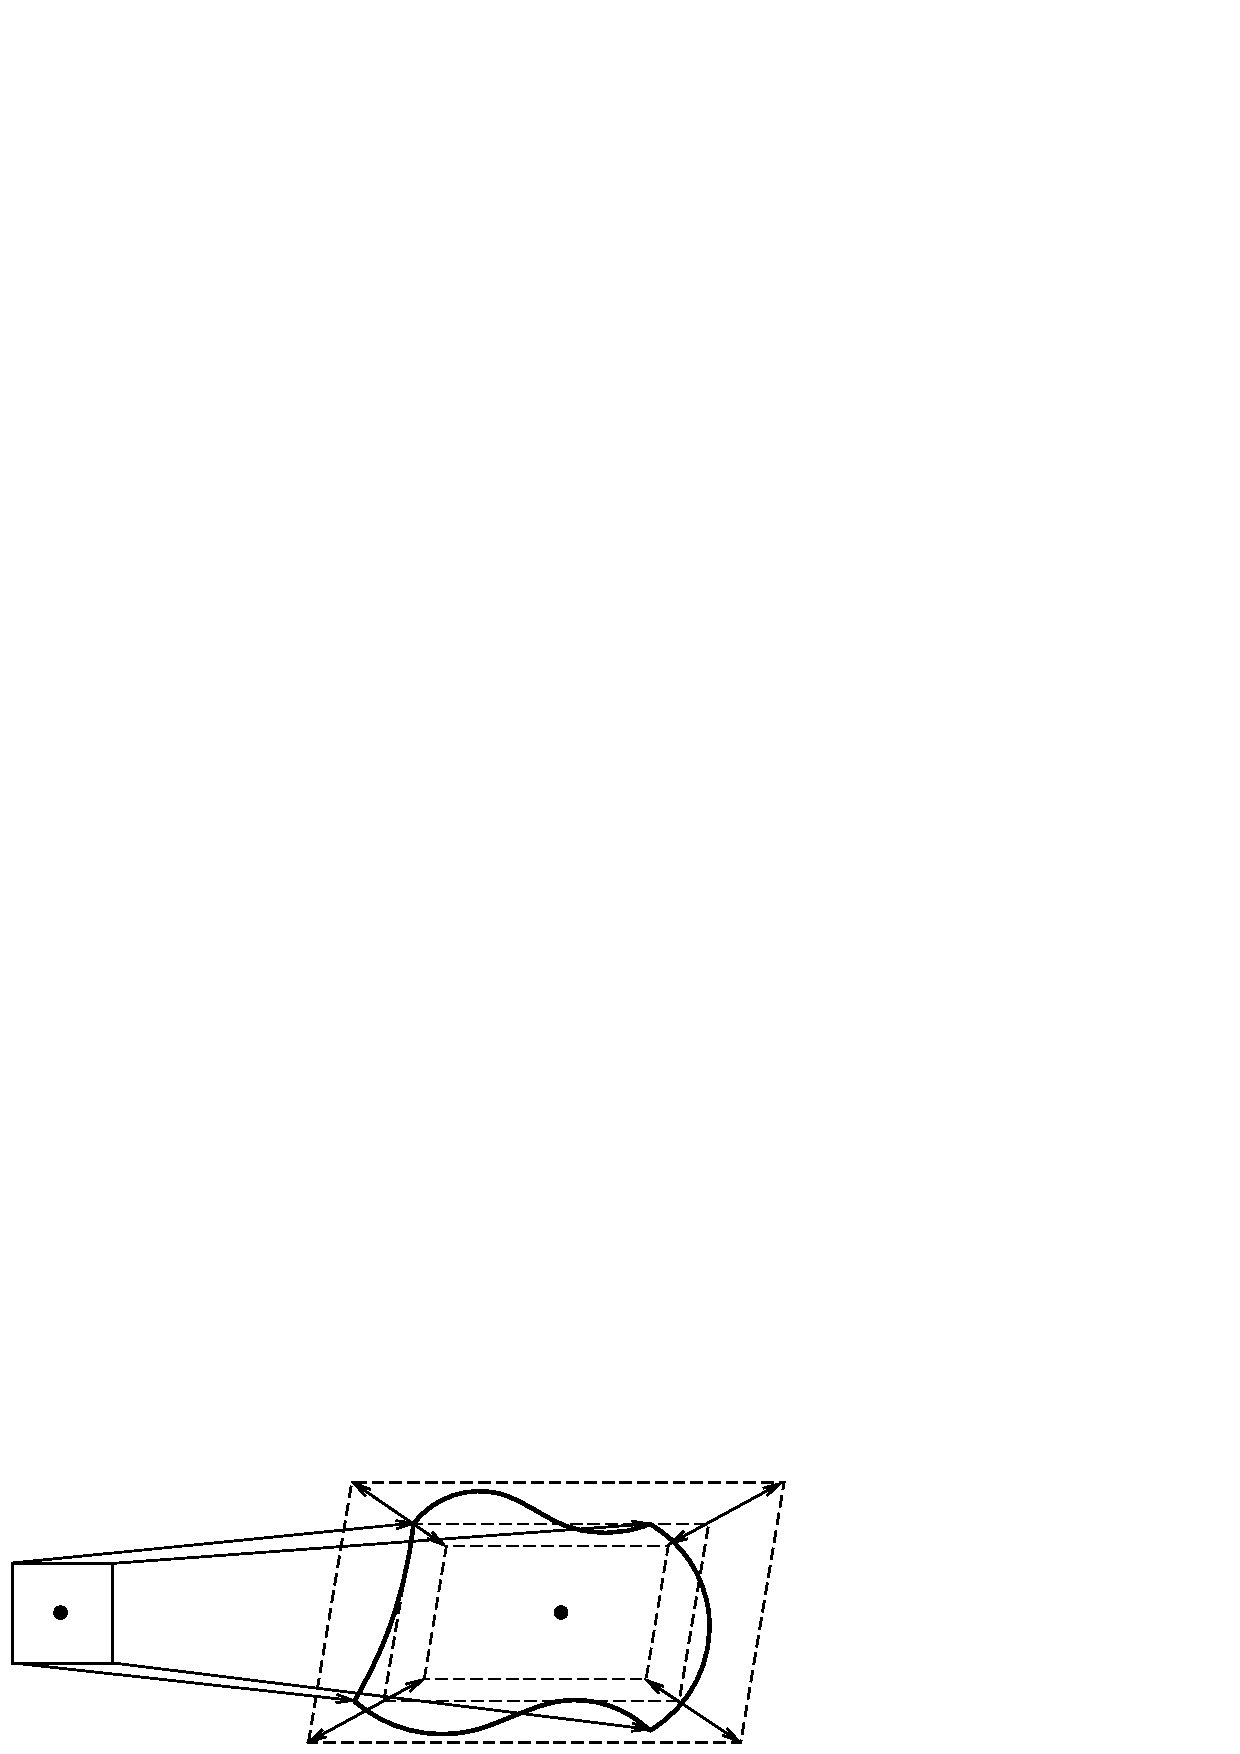
\includegraphics[width=3cm]{img/final/galat/1.pdf} разве можем не дойти до бесконечности? Почему нет? Мало ли бреда в~математике.

$\forall\  \e\hm>0\ \forall\  c\hm>0\pau \exists\  m\colon \e m\hm>c$. В~средние века сказали бы «клянусь честью дворянина».
 Также можем сказать: под~$\begin{sideways}
\Big[
\end{sideways}$ контролем, мамой клянусь, гадом буду.

\begin{Proof}
Пусть $\N\hm=\{1,1+1,1+1+1,\ldots\}$ ограниченно сверху, тогда у~этого множества существует точная верхняя грань ($\sup$).

$\sup \N\hm=c(\in \R)$.

\begin{enumerate}
    \item Предположим, что в~отрезке $[c-0{,}723,c]$ нет натуральных чисел $\hm{\imp}$ все натуральные числа меньше, чем $c-0{,}723 \hm{\imp} c-0{,}723$ "--- верхняя грань для $\N$. Противоречие с~тем, что $c$ "--- точная верхняя грань;
    \item Если же $\exists\  n\in [c-0{,}723,c]$, то $n+1\hm>c$, противоречие с~тем, что $c$ "--- верхняя грань.
\end{enumerate}
\end{Proof}

\section{Сравнение мощностей}

\begin{Def}
Множества $A$ и $B$ эквивалентны, если существует взаимнооднозначное отображение $A$ на~$B$.

\[A\sim B\]

Вспомним свойства отношения эквивалентности:

\begin{enumerate}
    \item $A\sim A$ "--- рефлексивность;

    \item $A\sim B \hm{\imp} B\sim A$ "--- симметричность;

    \item $A\sim B, B\sim C\hm{\imp} A\sim C$ "--- транзитивность.
\end{enumerate}
\end{Def}

\begin{Def}
Если множество $A$ эквивалентно некоторому подмножеству множества $B$, то говорят, что мощность $A$ не превосходит мощности $B$.
 То есть $A$ эквивалентно подмножеству $B \hm{\iff} \exists$ инъективное отображение $A$ в~$B$.

\end{Def}
$\card A\leq \card B$\pau $|A|\leq|B|$\pau $\#A\leq\#B$.

\begin{Ut} Свойства кардиналов:
\begin{enumerate}
    \item $\forall\  A,B\pau \card A\leq \card B$ или $\card B\leq \card A$ "--- доказываем целый семестр на~спецкурсе;

    \item Если $\card A\leq \card B$ и $\card B\leq \card A$, то~$A\sim B$ "--- теорема Кантора"--~Бернштейна;

    \item Если $\card A\leq \card B$ и $\card B\leq \card C$, то~$\card A\leq \card C$.
\end{enumerate}
\end{Ut}

\begin{Proof}(3)
    $\exists\ \phi\colon A\xrightarrow{\text{инъекция}}B,\
    \psi\colon B\xrightarrow{\text{инъекция}} C\hm{\imp} \psi\circ\phi\colon A\to C$ "--- тоже инъекция.
\end{Proof}

Кажется, началось. Мы честно признаёмся, что свойства 1 и 2 идут без доказательства.

\begin{Def}
Множество $A$ состоит из~$n$ элементов, если $A\sim\{1,2,3,\ldots,n\}$, то есть можем элементы пересчитать. Всего $n!$ способов пересчитать.
\end{Def}

\begin{Ut}
Если множество $A$ состоит из~$n$  элементов, $a\nin A$, то $A\cup \{a\}$ состоит из~$n+1$ элемента.
\end{Ut}

\begin{Proof} Рисунок \ref{dobvyk}.
\begin{figure}[htbp]\centering
    \includegraphics[width=3cm]{img/final/galat/7/mnpo.pdf}
    \includegraphics[width=3cm]{img/final/galat/7/mnm1.pdf}
    \caption{Добавление и выкидывание элементов}\label{dobvyk}
\end{figure}
\end{Proof}

\begin{Ut}
Если множество $A$ состоит из~$n$ элементов и $a\in A$ то $A\dd\{a\}$ состоит из~$n-1$ элемента.
\end{Ut}

\begin{Proof}
Пусть $a_n$ теперь соответствует $k$. А~можно и иначе: подвинуть $a_{k+1},\ldots,a_n$ на~одну позицию вверх.

Было: $\phi\colon A\Tot{вз-одн}\{1,\ldots,n\}$, $\phi(a)\hm=k$.

$\psi(b)\hm=\begin{cases}
    \phi(b),&\text{если } \phi(b)\hm<k;\\
    \phi(b)-1,&\text{если }\phi(b)\hm>k.
\end{cases}$

$\psi\colon A\lra\{1,\ldots,n\}$.
\end{Proof}

Ещё парочка определений:

\begin{Def}
Будем говорить, что пустое множество состоит из~нуля элементов.
\end{Def}

\begin{Def}
Множество называется конечным, если оно состоит из~$n$ элементов для некоторого $n\in \N\cup\{0\}\hm=\Z_+$.
\end{Def}

\begin{Def}
Множество называется бесконечным, если оно не является конечным.
\end{Def}

\begin{Def}
Множество называется счётным, если оно эквивалентно множеству $\N$.
\end{Def}

\begin{Def}
Множество называется \textbf{не более чем счётным}, если оно конечно или счётно.
\end{Def}

\begin{Ut}
Любое бесконечное множество имеет счётное подмножество.
\end{Ut}

\begin{Proof}
Пусть $A$ "--- бесконечное множество. Возьмём в~качестве $a_1$ произвольный элемент множества $A$. Положим $A_1\hm=A\dd\{a_1\}$.

$A_1\neq\q$, иначе $A$ конечно.

Возьмём в~качестве $a_2$ произвольный элемент $A_1$, положим $A_2\hm=A_1\dd\{a_2\}\hm=A\dd\{a_1,a_2\},\ A_2\neq\q$.

Предположим, что уже выбраны элементы $a_1,\ldots,a_n$, при этом
$A_n\hm=A\dd\{a_1,\ldots,a_n\}\pau A_n\neq\q$.
В~качестве $a_{n+1}$ выберем произвольный элемент $A_n$
$\big(a_{n+1}\nin\{a_1,\ldots,a_n\}\big)$, положим $A_{n+1}\hm=
A_n\dd\{a_{n+1}\}\hm=A\dd\{a_1,\ldots,a_{n+1}\}$. Индуктивно продолжим процесс, выбрав для каждого $n$ по~элементу.
 Получим подмножество $\{a_1,\ldots,a_k,\ldots\}$ "--- подмножество, эквивалентное $\N$.

Чтобы определение было корректно: раз у~нас $a_1,\ldots$ все попарно различны, значит, биективность с~$\N$ есть.
\end{Proof}

\textit{Скорость чтения лекции может резко возрасти. Я~вообще пишу на~доске, чтобы как-то себя затормозить.
 И когда лектор хорошо знает, чт\'{о} он сейчас будет рассказывать, он пишет быстро.
  Я хороший лектор, я~не~сразу понимаю, что рассказываю.}

Почти все теоремы сегодня Кантора.

\begin{The}\label{Kantor}
Объединение не более чем счётной совокупности не более чем счётных множеств не более чем счётно.
\end{The}

\textit{Ещё интереснее звучит такое, кстати очень серьёзное утверждение: «тощее множество не может быть полным».}

\textit{Давайте я, наконец, пожелаю всем собравшимся приятного аппетита, и мы продолжим.}

\begin{Proof}
Пусть $\big\{A_k\big\}_{k\hm=1}^{\mathcal{K}}$ ($\mathcal K\in\N\cup\{+\infty\}$) "--- не более
 чем счётная совокупность не более чем счётных множеств $A_k\hm=\{a_1^k,a_2^k,\ldots\}$.

Нужно их все прообъединять.

\pic{galat/7/usmn}{2}{trec}{Траектория}

 Табличка может быть бесконечной вправо, может быть бесконечной вниз.

 Не нравится ходить по~диагонали? Военные, например, любят, когда всё прямо и перпендикулярно.
 \pic{galat/7/usmnpr}{3}{ptrec}{Прямая траектория}


Будем нумеровать элементы $\bigcup\limits_k A_k$. Начинаем с~элемента $a_1^1$. Он будет первый,
 следующим будет номер два. Делаем шаги в~соответствии с~нарисованной траекторией.
  Если клетка пустая или содержит элемент, который уже встречался, то (ничего не делаем) и переходим на~следующую клетку, в~противном случае приписываем элементу
следующий номер и увеличиваем следующий номер на~единицу и переходим в~следующую клетку.

\pic{galat/7/mni}{2.2}{mni}{Шаги по~траектории}


Пройдём всё, потому что на~$a^j_i$ наступим за число шагов, которое можно найти.
\end{Proof}

\begin{Sl}
\begin{tabular}{llll}
$\Z$&счётно& &$\Z\hm=\N\cup(-\N)\cup\{0\}$ по~теореме \ref{Kantor} Кантора счётно;\\
$\Q$&счётно& &$\Q\hm=\bigcup\limits_{m\in\Z}\left(\bigcup\limits_{n\in \N}\left\{\dfrac mn\right\}\right)$;\\ $\mathbb{A}$&счётно& &
\end{tabular}
\end{Sl}

\begin{Proof} Действительно: $\left\{\dfrac mn\right\}$ "--- конечное множество из~одного элемента. $\bigcup\limits_{n\in\N}$ "--- счётное объединение. $\bigcup\limits_{m\in\Z}$ "--- счётное объединение. В~итоге после всех объединений множество не более чем счётно.

$\mathbb{A}\hm=\{x\in\R\colon x$ является корнем хоть одного многочлена с~рациональными коэффициентами (всё равно, что с~целыми)$\}$.

\begin{enumerate}
    \item Многочленов степени $n\in\N$ с~фиксированными коэффициентами не более чем счётное множество:
        $\bigcup\limits_{a_n\in\Z}\Big(\dots\bigcup\limits_{a_1\in\Z}\bigcup\limits_{a_0\in\Z}\Big)\{a_nx^n+a_{n-1}x^{n-1}+\ldots+a_1x+a_0\}$;

    \item Множество чисел, являющихся корнями многочлена степени $n\in \N$, конечно, то есть не более чем счётно;

    \item Теперь, объединяя по~$n$ такие множества, получим множество $\mathbb{A}$. Такое гигантское множество, оказывается, тоже счётно.
\end{enumerate}
\end{Proof}

Давайте я~ещё какие-нибудь теоремы напишу.

\begin{Ut}
Подмножество не более чем счётного множества не более чем счётно.
\end{Ut}

\begin{Proof}
$a_1,a_2,\underbrace{a_3}_{b_1},a_4,\ldots\underbrace{\ldots}_{b_2}\ldots$

Идём слева направо и нумеруем.
\end{Proof}

\begin{Ut}
Если $A$ бесконечно, а~$B$ не более чем счётно, то $A\cup B\sim A$.
\end{Ut}

\begin{Proof}
Пусть $A_1$ "--- счётное подмножество $A$, а~$B_1\hm=B\dd A$ не более чем счётно.

$A\cup B\hm=(A\dd A_1)\cup(A_1\cup B_1)$.

Если $A_1\sim B_1,\ A_2\sim B_2, A_1\cap A_2\hm=\q, B_1\cap B_2\hm=\q$, то $(A_1\cup A_2)\sim (B_1\cup B_2)$ "--- это лирика.

\pic{galat/7/er}{1.5}{er}{Эквивалентность объединения непересекаемых}

Итак: $A\cup B\hm=\underset{\sim A\dd A_1}{(A\dd A_1)}\cup
\underset{\sim A_1}{(A_1\cup B_1)}\sim (A\dd A_1)\cup A_1\hm=A$.
\end{Proof}

Оказывается, добавлять "--- глупый процесс. Выкидывать гораздо интереснее.
\section{Бесконечные множества}

Вспомним важное:

\begin{enumerate}
\item $A\sim B\hm{\iff}\exists\  \phi\colon A\Tot{вз-одн}B$.

\item Если $A\sim B_0\subset B, B\sim A_0\subset A$, то $A\sim B$.

\item Любое бесконечное множество имеет счётное подмножество.

\item Объединение не более чем счётной совокупности не более чем счётных множеств не более чем счётно.

\item Если $A_1\sim B_1,A_2\sim B_2,A_1\cap A_2\hm=\q,B_1\cap B_2\hm=\q$,
то $(A_1\cup A_2)\sim (B_1\cup B_2)$.

\item Если $A$ бесконечно, $B$ не более чем счётно, то $(A\cup B)\sim A$.
\end{enumerate}
\begin{Proof}
    $A\cup B\hm=A\cup(B\dd A)$, где $(B\dd A)$ не более чем счётно. 
    $\underset{\sim A\dd A_1}{(A\dd A_1)}\cup\underset{\sim A_1}{\big(A_1\cup( B\dd A)\big)}$.
\end{Proof}

Что можно выкидывать безболезненно?

\begin{Ut}
Если $A$ "--- бесконечное множество, $B$ "--- конечное подмножество $A$, то $A\dd B\sim A$.
\end{Ut}

\begin{Proof}
С~учётом индукции достаточно доказать, что $\forall\  a\in A\pau A\dd\{a\}\sim A$ (индукция применяется только для конечного числа выкидываний).

$A\dd \{a\}$ бесконечно (если оно конечно из~$n$ элементов, то $A$ из~$n+1$ тоже конечное, противоречие).

Пусть $A_1$ "--- бесконечное счётное подмножество $A\dd \{a\}$ (которое бесконечно, поэтому и имеет счётное подмножество).

Что такое вообще множество $A$? $A\hm=\Big(A\dd\big(A_1\cup\{a\}\big)\Big)\cup\Big(A_1\cup\{a\}\Big)$.

Глубокий факт: $\Big(A\dd \big(A_1\cup\{a\}\big)\Big)$ эквивалентно себе, а~$\big(A_1\cup\{a\}\big)\sim A_1$.

$A\dd\big(A_1\cup\{a\}\big)\cup\big(A_1\cup\{a\}\big)\sim
\Big(A\dd\big(A_1\cup\{a\}\big)\Big)\cup A_1\hm=
A\dd\{a\}$.
\end{Proof}

\textit{Бесконечная государственная казна, из~которой чиновники берут конечные суммы и знают, что бесконечность остаётся такой же.}


\[(a,b)\sim[a,b]\sim[a,b)\sim(a,b]\sim\left[0;\textstyle\frac{\pi}2\right)\sim\R^+\]

$(0,1)\overset{\underset{/}{\text{ну}}\text{ лин от-ние}}
{\sim\left(-\frac{\pi}2,\frac{\pi}2\right)}\overset{\tg}{\sim}\R
\mspace{72mu}
\phi(x)\colon (0,1)\to(a,b)\mspace{72mu}\phi(x)\hm=x(b-a)$.

\pic{galat/8/sim}{1}{simr}{Гомотетия}



\pic{galat/8/trkv}{3.6}{trkv}{Фигуры на~плоскости эквивалентны}


\begin{Ut}Точек в~квадрате ровно столько же, сколько в~отрезке.

\[
[0,1]\sim[0,1]^2
\]\end{Ut}

\begin{Proof}
    $\card[0,1]\leq\card[0,1]^2$, задать биективное отображение с~подмножеством квадрата, тривиально.

    Покажем, что $\card[0,1]^2\leq\card[0,1]$.

    Возьмём точку квадрата $(x,y)\hm=(0{,}n_1^xn_2^x\ldots,0{,}n_1^yn_2^y\ldots)$ "--- координаты в~десятичной записи.
     Зададим инъективное отображение, при котором точка $(x,y)$ перейдёт в~$(0{,}n_1^xn_1^y2n_2^xn_2^y2n_3^xn_3^y\ldots)$.

    Проблема: $0{,}111111\ldots,0{,}1\underset{\text
    {запрещённые девятки}}{9999999999999999999}\ldots\to0{,}112192192192\ldots$ "--- ни один
     образ не будет содержать периодическую девятку с~таким порядком записи. Итак, мы установили взаимнооднозначное
      отображение множества точек квадрата на~подмножество (ведь есть точки ещё и без двоек через каждые три цифры, например) отрезка.

    Применяем теорему Кантора"--~Бернштейна и всё, собственно.
\end{Proof}

Фундаментальная теорема математики была бы о~том, что бесконечность везде одинакова. Но это не так.

\begin{The}
    $[0,1]$ "--- не счётное множество.
\end{The}

\begin{Proof}\textbf{1.}

    Пусть $\phi$ "--- инъективное отображение $\N\to[0,1)$. Достаточно показать, что оно не сюръективное.
    Введём следующие обозначения: пусть $\phi(n)\hm=0{,}k_1^nk_2^nk_3^n\ldots$ (запись без периодических девяток).

    Пусть $x\hm=0{,}a_1a_2a_3a_4\ldots$, где $a_j\hm=
    \begin{cases}
        3,&\text{если } k_j^j\neq3\\
        7,&\text{если } k_j^j\hm=3
    \end{cases}$ (периодическая девятка невозможна).

    $\forall\  j\in\N\pau x\neq\phi(j)$ "--- отличие по~крайней мере в~$j$-ом разряде, а~периодическая девятка запрещена.
    Значит, $\phi$ не сюръективно (ну и не биективно). Чуть подробнее: у~нас есть образ $\phi(\N)$, он состоит из~кучи действительных чисел
    $\phi(1),\phi(2),\ldots$. Глядя на~эти $\phi(j)$ строим «плохое» число: ноль целых и что-то после запятой. 
    Первую цифру после запятой ставим не такую, как в~$\phi(1)$, вторую "--- не такую, как в~$\phi(2)$ и так далее.
     Это число не будет равняться никакому $\phi(j)$, но оно точно есть в~$[0,1]$ и без периодических девяток, 
     потому что там исключительно $3$ или $7$. Вот и развалилась сюръективность.

\end{Proof}

$\begin{matrix}
    \phi(1)\hm=&0{,}\boxed{k_1^1}k_2^1k_3^1\ldots\\
    \phi(2)\hm=&0{,}k_1^2\boxed{k_2^2}k_3^2\ldots\\
    \phi(3)\hm=&0{,}k_1^3k_2^3\boxed{k_3^3}\ldots\\
    \ldots&\ldots\ldots
\end{matrix}$ "--- в~рамках "--- цифры, которые не дают совпасть $\phi(j)$ с~заданным иксом.

\begin{Proof}\textbf{2}

    Пусть $\phi(n)$ "--- произвольное инъективное отображение $\N\to [0,1]$. Достаточно доказать, что $\phi$ не сюръективно.


    \pic{galat/8/otr}{1.35}{otr}{Отрезок}



    Обозначим $\phi(n)$ через $x_n$. Положим $\Delta_0\hm=[0,1]$. В~качестве $\Delta_1$
     выберем произвольную треть (являющуюся именно отрезком) отрезка $\Delta_0$, не содержащую $x_1$.
\pic{galat/8/delta1}{1.35}{delta1}{Выбор вложенного отрезка}


Если уже построен отрезок $\Delta_n$, то в~качестве отрезка $\Delta_{n+1}$ берём произвольную треть
 отрезка $\Delta_n$, не содержащую $x_{n+1}$. Построена последовательность вложенных отрезков $\Big\{\Delta_n\Big\}_{n\hm=0}^{\infty}$.

В~соответствии с~принципом Кантора \ref{ppk} о~вложенных отрезках существует общая точка этих отрезков,
 обозначим её за $x$. Ни для одного $n\in\N\pau x\neq x_n\hm=\phi(n)\pau x\in\Delta_n\nni x_n$.


\end{Proof}

\textit{Отношение к~хлебу определяет моральный облик общества.}

\begin{Def}
    Множества, эквивалентные $[0,1]$, называются \textbf{континуальными}.
\end{Def}

\begin{Sl}
    Множества иррациональных чисел континуально. Множество трансцендентных (то есть не алгебраических) чисел тоже континуально.
\end{Sl}

\begin{Proof}
    В~любом отрезке существует хоть одно иррациональное число; кроме того, их бесконечное множество.
     Факт нетривиальный. Давайте смотреть: если это множество не более чем счётно, то


    $\text{Отрезок}\hm=\underset{\text{счётно}}{\{\text{множество рациональных чисел отрезка}\}}\cup\{$множество иррациональных чисел отрезка$\}\hm{\imp}$ Отрезок "---счётное множество.

    Или ещё так: $\underset{\text{беск}}{\Big([0,1]\dd \Q\Big)}\cup\underset{\text{сч.}}{\Q}\sim[0,1]\dd \Q$.
\end{Proof}


Пусть $A$ "--- счётное множество. $\mathscr A$ "--- совокупность всех его подмножеств.

\begin{The}[Кантора]\label{KAn}
$\card A\hm<\card\mathscr A$.
\end{The}

\begin{Proof}
    \begin{enumerate}
        \item Инъективное отображение $A\to \mathscr A$\pau $a\to\{a\}\hm{\imp}\card A\leq\card \mathscr A$ "--- тривиальная часть;

        \item Покажем, что $\card A\hm<\card\mathscr A$. Пусть $\phi$ "--- произвольное инъективное отображение $A\to \mathscr A$. Достаточно показать, что оно не сюръективно.
            Обозначим образ $\phi(a)$ через $A_a$;

            Положим, что множество $B\hm=\Big\{a\in A\colon a\nin A_a\Big\}$. Ни для одного элемента $a\in A$ множество $B$ не совпадает с~$A_a$. Почему? а~вот, почему:
    \end{enumerate}

            Пусть $a$ "--- произвольный элемент $A$. Покажем, что $B\neq A_a$. Действительно, пусть $B\hm=A_a$ для некоторого $a_0\in A$, тогда

            \begin{enumerate}
                \item $a_0\in A_{a_0}(\hm=B)\hm{\imp} a_0\nin B$ (принадлежит $A_{a_0}$, значит, \textbf{не должен} принадлежать $B$). Одновременно входит и не входит;

                \item $a_0 \nin A_{a_0}(\hm=B) \hm{\imp} a_0$ должен принадлежать $B$.
            \end{enumerate}

            Мораль: противоречие.

\end{Proof}

\section{О~точках}
\begin{Def}
    Двузначная последовательность "--- последовательность двух элементов множества.
\end{Def}

$\ro$ "--- множество всех последовательностей из~$0$ и $1$.

\begin{Ut}
    $\ro$ континуально. (то есть $\ro\sim[0,1]$).
\end{Ut}

\begin{Proof}
    \begin{enumerate}
        \item Пусть $x$ "--- произвольное число отрезка $[0,1]$.

            Запишем $x$ в~двузначной записи $x\hm=0{,}n_1n_2n_3n_4\ldots\pau \big(n_i\in\{0,1\}\big)$. Для тех, кому не нравятся $0$ и $1$, пишем «лево» и «право».


\pic{galat/9/levo}{1.2}{levo}{Альтернатива нулям и единицам в~отрезке}

Соответственно, $[0,1]\ni x\to \underset{\in\ro}{n_1n_2n_3}\ldots$ инъективно. Значит, $\card [0,1]\leq\card\ro$.

Для $\frac 12\to\begin{cases}
    0{,}10000\\
    0{,}01111\ldots
\end{cases}$ "--- но мы выберем одно, задавая отображение $\hm{\imp}$ не биективно.

\item Пусть $n_1n_2n_3\ldots\in\ro$. Сопоставим ей число $x$ отрезка $[0,1]$.

    $x\hm=0{,}n_1n_2n_3\ldots$ "--- десятичная запись (я же не хочу получить все числа, $n$ здесь "--- только $1$ или $0$).

    Это инъективное отображение $\ro$ в~$[0,1]$. Мощность $\card\ro\leq\card[0,1]$. По~теореме Кантора"--~Бернштейна вывод: $\card\ro\hm=\card[0,1]$.
    \end{enumerate}
\end{Proof}

\subsection{А~теперь рассмотрим подмножества расширенной прямой}

Пусть $x$ "---точка действительной прямой, а~$\e\hm>0$.

\begin{Def}
    $\e$-окрестностью точки $x$ называется интервальчик $(x-\e,x+\e)$. Обозначается $B_\e(x)$.

    Проколотая $\e$-окрестность точки $x\colon(x-\e,x+\e)\dd\{x\}$. Обозначается $B'_\e(x)$.

    На~$\R\colon B_\e(+\infty)\hm=B'_\e(+\infty)\hm=\big(\frac{1}{\e},+\infty\big)$ "---
    \textup{(}$\frac 1\e$ чтобы при увеличении $\e$ окрестность сужалась\textup{)}. $B_\e(-\infty)\hm=(-\infty,-\frac 1\e)$.

    На~$\ol\R\colon B_\e(+\infty)\hm=\big(\frac{1}{\e},+\infty\big],B'_\e(+\infty)\hm=\big(\frac{1}{\e},+\infty\big)$. Для $-\infty$ аналогично.
\end{Def}

Окрестность "--- субъективно маленький интервал.

Пусть $A\subset\R(\ol\R)$.

\begin{Def}
    Точка $x$ называется внутренней точкой множества $A$, если $x$ входит в~$A$  с~некоторой своей окрестностью, то есть
    \[ \exists\ \e\hm>0\colon B_\e(x)\subset A.\]
\end{Def}

\begin{Def}
    Точка $x$ называется внешней точкой множества $A$, если $x$ входит в~дополнение $A$ с~некоторой своей окрестностью, то есть
    \[ \exists\  \e\hm>0\colon B_\e(x)\cap A\hm=\q.\]
\end{Def}

\begin{Def}
    Точка $x$ называется \textbf{граничной} точкой множества $A$, если она не является ни внутренней, ни внешней, то есть
    \[\forall\  \e\hm>0\pau B_\e(x)\cap A\neq\q, B_\e(x)\cap\ol A\neq\q.\]
    $\ol A\hm=\R\dd A$ или $\ol\R\dd A$.
\end{Def}

\begin{Def}
    Точка $x$ называется изолированной точкой множества $A$, если $\exists\ \e\hm>0\colon B_\e(x)\cap A\hm=\{x\}$.
\end{Def}

\begin{Def}
    Множество $A$ называется открытым, если все его точки внутренние. То есть
    \[  \forall\  x\in A\pau\exists\  \e\hm>0\colon B_\e(x)\subset A.    \]
\end{Def}

\begin{Def}
    Множество $A$ называется замкнутым, если его дополнение открыто.
\end{Def}

Интервал "--- открытое множество, отрезок "--- замкнутое; полуотрезок, рациональные числа "--- никакие множества. Подмножества отрезка составляют гиперконтинуум, замкнутые множества "--- континуум.

$\q,\R$ и открыты и замкнуты.

\subsubsection*{Почему других открытых и замкнутых нет?} Можно делить отрезки пополам; если обе половины открыты, то одна точка окажется между.

\subsubsection{Свойства}

\begin{Ut}
    Множество открыто $\hm{\iff}$ оно не содержит ни одной граничной точки.
\end{Ut}

\begin{Ut}
    Множество замкнуто $\hm{\iff}$ оно содержит все свои граничные точки.
\end{Ut}

\begin{Pre}
    Точка $x$ является граничной точкой $A \hm{\iff}x$ является граничной точкой $\ol A$.
\end{Pre}

Вариант-исключение, когда граничных точек нет.

$\ol{\ol A}\hm=\ol{(\ol A)}\hm=A$

\begin{Ut}
    Объединение \textbf{произвольной} совокупности открытых множеств "--- открытое множество. Пересечение \textbf{конечной} совокупности открытых множеств "--- открытое множество.
\end{Ut}

Если издеваться, но не сильно, открытость сохраняется.

\begin{Proof}
    Пусть $\Big\{G_\lambda\Big\}_{\lambda\in\Lambda}$
    "--- совокупность открытых множеств. $x$ "--- произвольная точка из~$\bigcup\limits_{\lambda\in\Lambda}G_\lambda$.
    Тогда $\exists\ \lambda_0\colon x\in G_{\lambda_0}$;
    так как $G_{\lambda_0}$ открытое, $\exists\ \e\hm>0\colon B_\e(x)\subset G_{\lambda_0}
    \hm{\imp} B_\e(x)\subset\bigcup\limits_{\lambda\in\Lambda}G_\lambda$. Значит, $\bigcup\limits_{\lambda}G_\lambda$ открыто.

    Пусть $C_1\ldots,C_N$ открыты. $x$ "--- произвольная точка
    $\bigcap\limits_{n\hm=1}^{N}C_n\hm{\imp}$

    $\hm{\imp} x\in C_1\hm{\imp}\exists\  \e_1\hm>0\colon B_{\e_1}(x)\subset C_1$

    $x\in C_2\hm{\imp}\exists\ \e_2\hm>0\colon B_{\e_2}(x)\subset C_2$

    $\vdots$

    $x\in C_N\hm{\imp}\exists\ \e_N\hm>0\colon B_{\e_N}(x)\subset C_N$

    Положим $\e\hm=\min\{\e_1,\ldots,\e_N\}$ "--- в~конечном наборе наименьший точно найдётся (именно поэтому верно только для пересечения конечной совокупности).

    Тогда $\forall\  n\in\{1,\ldots,N\}\pau B_\e(x)\subset C_n\hm{\imp} B_\e(x)\subset
    \bigcap\limits_{n\hm=1}^NC_n$. Значит, $\bigcap\limits_{n\hm=1}^NC_n$ открыто.
\end{Proof}

Бесконечное пересечение ведёт себя по-разному: иногда хорошо:
$\bigcap\limits_{n\in \N}\left(-\dfrac1n,1+\dfrac1n\right)\hm=[0,1]$,
иногда не очень:
 $\bigcap\limits_{n\in \N}\left(-\dfrac1n,1\right)\hm=[0,1)$.

 \begin{Sl}
Пересечение \textbf{произвольной} совокупности замкнутых множеств замкнуто. Объединение \textbf{конечной} совокупности замкнутых множеств "--- замкнутое множество.
 \end{Sl}

 \begin{Proof}
$\Big\{\mathcal{F}_\lambda\Big\}_{\lambda\in\Lambda}$ "--- совокупность замкнутых множеств.
$\bigcap\limits_{\lambda\in\Lambda}\mathcal{F}_\lambda\underset{\ref{Themor}}{\hm=}
\bigcup\limits_{\lambda\in\Lambda}\ol{{\mathcal F}_\lambda}$ "--- объединение открытых множеств открыто.
 \end{Proof}

 \begin{Def}\label{pt}
Точка $x$ называется предельной точкой множества $A$, если в~любой проколотой окрестности $x$ есть хоть одна точка множества $A$, то есть
\[  \forall\  \e\hm>0\pau B'_\e(x)\cap A\neq \q.\]
 \end{Def}

 \begin{The}\label{hal}
Следующие утверждения эквивалентны:
\begin{enumerate}
    \item $x$ "--- предельная точка $A$.
    \item $\forall\  \e\hm>0\ B'_\e(x)\cap A$ "--- бесконечное множество.
    \item $\forall\  \e\hm>0\ B_\e(x)\cap A$ "--- бесконечное множество.
\end{enumerate}
 \end{The}

 \begin{Proof}
$2\hm{\iff} 3$ "--- это понятно, они отличаются максимум на~одну точку.

$2\hm{\imp} 1$ халява: по~определению.

Осталось $1\hm{\imp} 2$. От противного для скорости: пусть $\exists\ \e\hm>0\colon B'_\e(x)\cap A$ конечно. Пусть это пересечение состоит из~точек $\big\{a_1,\ldots,a_N\big\}$. Положим $\e_0\hm=\min\big\{|x-a_1|,|x-a_2|,\ldots,|x-a_N|\big\}\hm>0$.

Тогда $B'_{\e_0}(x)\cap A\hm=\q$ "--- противоречие с~тем, что $x$ есть предельная точка.
 \end{Proof}

 \begin{Ut}
Множество замкнуто $\hm{\iff}$ оно содержит все свои предельные точки.
 \end{Ut}

 \begin{Proof}
Пусть $A$ "--- замкнуто, $x\nin A$. Достаточно доказать, что $x$ не предельная точка.

Так как $A$ замкнуто, $x$ "--- внешняя точка $A$, то есть
 $\exists\ \e\hm>0\colon B_\e(x)\cap A\hm=\q$, значит $x$ не предельная точка.

 Пусть $A$ содержит все свои предельные точки. Покажем, что $A$ замкнуто.
 Пусть $x$ "--- произвольная точка из~$\ol A$. Тогда $x$ не предельная точка $A$.

 $\exists\ \e\hm>0\colon B'_\e(x)\cap A\hm=\q$. Так как $x\nin A$, то $B_\e(x)\cap A\hm=\q$, то есть $x$ "--- внешняя точка $A$. Следовательно, $\ol A$ открыто; $A$, стало быть, замкнуто.
 \end{Proof}

 \section{Теорема Больцано"--~Вейерштрасса}

 Мы работаем с~множеством $A\subset\R(\ol\R)$.

 \begin{Def}
$x$ "--- предельная точка $A$, если $\forall\ \e\hm>0$ пересечение $B'_\e(x)\cap A\neq \q$ (или, эквивалентно, $\forall\  \e\hm>0\ B'_\e(x)\cap A$) бесконечно.
 \end{Def}

 \begin{The}[Больцано"--~Вейерштрасса о~существовании предельной точки]\label{bolc} Любое бесконечное ограниченное подмножество  $\R$ имеет (хоть одну) предельную точку на~$\R$.
\end{The}

\begin{Proof}
    Метод имени Цезаря: Пусть $A$ "--- произвольное бесконечное ограниченное подмножество $\R$. Найдём $c\hm>0\colon A\subset[-c,c]$ (используем ограниченность).
    Положим $\Delta_0\hm=[-c,c]$.

    Метод copy-paste. В~качестве отрезка $\Delta_1$ возьмём произвольную половину $\Delta_0\colon A\cap \Delta_1$ бесконечно. В~качестве $\Delta_2$ возьмём произвольную половину $\Delta_1\colon A\cap\Delta_2$ бесконечно "--- и так далее.

    Если уже построен $\Delta_n\colon A\cap \Delta_n$ бесконечно, то в
    качестве $\Delta_{n+1}$ возьмём произвольную половину $\Delta_n\colon \Delta_{n+1}\cap A$ бесконечно.

    Получили последовательность вложенных отрезков: $\Big\{\Delta_n\Big\}_{n\hm=0}^{\infty}\colon \forall\  n\in \N\pau A\cap\Delta_n$ бесконечно. $|\Delta_n|\hm=\dfrac{2c}{2^n}$.

    Докажем такую лемму:

    \begin{Th}\label{perednosom}
        $\forall\ \e\hm>0\pau \forall\  \tilde c\hm>0\pau \exists\ \ N\in\N\colon \forall\  n\hm>N\pau \dfrac{\tilde c}{2^n}\hm<\e$
    \end{Th}

    \begin{proof}
        Найдём $N\hm>\dfrac{\tilde c}{\e}$ (используем принцип \ref{arhy} Архимеда).
         
Тогда $\forall\  n\hm>N\pau 2^n\hm>2^N\hm=(1+1)^N\underset{\ref{Bern}}{\geq} 1+N\cdot1\hm>N\hm>\dfrac{\tilde c}{\e}$.

        Отсюда $\dfrac{\tilde c}{2^n}\hm<\e$.
    \end{proof}

    По~принципу \ref{ppk} Кантора $\exists\  x_0$ общая точка $\Big\{\Delta_n\Big\}_{n\hm=0}^\infty$. Покажем, что точка $x_0$ предельная точка $A$.

\pic{galat/10/dance}{2.5}{dance}{Танец отрезка в~окрестности}
    По~определению возьмём произвольное $\e\hm>0$. Найдём $n\colon \dfrac{2c}{2^n}\hm<\e$ (по лемме, которая перед носом). Тогда $\Big(B_\e(x_0)\cap A\Big)\supset\Big(\Delta_n\cap A\Big)$ "--- а~последнее бесконечно.

    %$\Biggl($А~это тут что вообще? %$\lambda\left[x_0,\dfrac{2c}{2^n}\right]+(1-\lambda)\left[-\dfrac{2c}{2^n},x_0\right],\pau %\lambda\in[0,1]\Biggr)$

    $\hm{\imp} x_0$ "--- предельная точка $A$.
\end{Proof}

\begin{The}
    Любое бесконечное подмножество $\ol{\R}$ имеет (хотя бы одну) предельную точку на~$\ol\R$.
\end{The}

\begin{Proof}
    \begin{enumerate}
        \item Достаточно рассматривать случай подмножеств обычной $\R$.

        \item
        \begin{enumerate}
            \item $A$ "--- ограниченное подмножество $\hm{\imp}$ имеет предельную точку на~$\R\hm{\imp}$ на~$\ol{\R}$ тем более.

            \item Неограниченное сверху множество: $+\infty$ является предельной точкой, снизу "--- $-\infty$.
        \end{enumerate}
    \end{enumerate}
\end{Proof}

\begin{Def}
    Система множеств $\Big\{G_\lambda\Big\}_{\lambda\in\Lambda}$ называется покрытием множества $A$, если $\bigcup\limits_{\lambda\in\Lambda}G_\lambda\supset A$. Покрытие называется открытым, если все $G_\lambda$ открыты.
\end{Def}

\begin{Def}
    Множество $A$ "--- подмножество действительной прямой, "--- называется компактным, если из~любого его открытого покрытия можно выделить конечное подпокрытие.

    То есть $\forall$ открытого покрытия $\Big\{G_\lambda\Big\}_{\lambda\in\Lambda}$ множества $A$ $\exists$ конечный набор индексов
    $\lambda_1,\ldots,\lambda_N\colon A\hm\subset(G_{\lambda_1}\cup\ldots\cup G_{\lambda_N})$.
\end{Def}

Пусть в~качестве $A$ будет интервал $(0,1)$.

$G_n\hm=\left(\dfrac1n,1-\dfrac1n\right)$ Нельзя конечным числом множеств $G_n$ покрыть $(0,1)$. Значит $(0,1)$ некомпактный.

\begin{Th}\label{kompogr}
    Если множество компактно, то оно ограниченно.
\end{Th}

\begin{Proof}
    Пусть $G_n\hm=(-n,n)$. $\bigcup\limits_{n\in\N}G_n\hm=\R\supset A$ "--- рассматриваемое компактное множество.
    в~силу компактности $\exists\  n_1,\ldots,n_k\colon G_{n_1},\ldots,G_{n_k}$ является покрытием $A$.

    Положим $N\hm=\max\{n_1,\ldots,n_k\}$ "--- выберем самый большой интервал. Значит, $A\subset G_N\hm=(-N,N)\hm{\imp} A$ "--- ограничено.
\end{Proof}

\begin{Th}\label{kompzam}
    Если множество компактно, то оно замкнуто.
\end{Th}

\begin{Proof}
    Пусть $x$ "--- произвольная точка $\R\dd A$ "--- рассматриваемое множество. Положим

    $G_n\hm=\left(-\infty,x-\frac1n\right)\cup\left(x+\frac1n,+\infty\right)$.
    $G_n\hm=\R\dd\left[x-\frac1n,x+\frac1n\right]$

    $\bigcup\limits_{n\in\N}G_n\hm=\R\dd\{x\}\supset A$ "--- ведь $x$ в~$A$ не содержится.

    Используя компактность выделим конечное подпокрытие $G_{n_1},\ldots,G_{n_k}$. Положим $N\hm=\max\{n_1,\ldots,n_k\}$.

    Тогда $A\subset G_N\hm=\R\dd \left[x-\frac1N,x+\frac1N\right]$. Значит $B_{\frac1N}(x)\subset\R\dd A$ "--- вместе с~любой точкой $x$
    в~дополнении множества $A$ ($\R\dd A$) лежит вся окрестность $B_{\frac1N}(x) \hm{\imp}$ дополнение открыто $\hm{\imp}$ $A$ "--- замкнуто.
\end{Proof}

\begin{The}[Гейне"--~Бореля"--~Лебега]\label{GBL}
    Отрезок "--- компакт.
\end{The}

\begin{Proof}
    Рассмотрим произвольный отрезок $[a,b]$. Пусть $\Big\{G_\lambda\Big\}_{\lambda\in\Lambda}$ "--- произвольное открытое покрытие $[a,b]$.

    От противного: предположим, что из~этого покрытия нельзя выделить конечное подпокрытие.
    Положим $\Delta_0\hm=[a,b]$. Дальше в~качестве отрезка $\Delta_1$ возьмём произвольную половину отрезка $\Delta_0$, для которой из~$\Big\{G_\lambda\Big\}_{\lambda\in\Lambda}$ нельзя выделить конечное подпокрытие.
    в~качестве $\Delta_2$ возьмём половину $\Delta_1$\ldotst{}

    Если уже построен отрезок $\Delta_n$ такой, что из~нашего покрытия нельзя выделить конечное подпокрытие,
     то в~качестве отрезка $\Delta_{n+1}$ возьмём половину $\Delta_n$, для которой из~$\Big\{G_\lambda\Big\}_{\lambda\in\Lambda}$
     нельзя выделить конечное подпокрытие.

    В~результате построена последовательность вложенных отрезков $\big\{\Delta_n\big\}_{n\hm=1}^\infty\pau \left(|\Delta_n|\hm=\dfrac{b-a}{2^n}\right)$.
            по~принципу полноты Кантора (теорема \ref{ppk}) $\exists\  x_0$ "--- общая точка отрезков.
            $\exists\ \lambda_0\in\Lambda\colon G_{\lambda_0}\ni x_0$, а~так как $G_{\lambda_0}$ "--- открытое множество,
            $\exists\  \e\hm>0\colon B_\e(x_0)\subset G_{\lambda_0}$.
            Дальше $\exists\  n\in \N\colon |\Delta_n|\hm=\dfrac{b-a}{2^n}\hm<\e$ (в~силу леммы \ref{perednosom} $\tilde c\hm=b-a$). Тогда
    $\Delta_n\subset B_\e(x_0)\subset G_{\lambda_0}\hm{\imp}\Delta_n\subset G_{\lambda_0}$ "--- противоречие с~тем, что для $\Delta_n$ нельзя выделить конечное подпокрытие.
\end{Proof}

Как ещё можно доказать теорему \ref{bolc} Больцано"--~Вейерштрасса.

\begin{Proof}\label{bolcproof}
    $A$ "--- бесконечное подмножество отрезка $[-c,c]$, не имеющее предельных точек. Для каждой точки $x\in[-c,c]$ найдём $\e_x\hm>0\colon
    B_{\e_x}(x)\cap A$ конечно. Рассмотрим $\Big\{B_{\e_x}(x)\Big\}_{x\in[-c,c]}$ "--- открытое покрытие $[-c,c]$. Отрезок "--- компакт, выделим конечное подпокрытие. Оно покрывает $A$, но состоит из~конечного набора множеств, в~каждом из~которых лишь конечное число точек $A\hm{\imp}$ противоречие с~бесконечностью множества $A$.

\end{Proof}

\section{О~последовательностях}

Важная теорема:

\begin{The}[Критерий компактности]\label{kk}
        Пусть $A\subset\R$. Следующие утверждения эквивалентны:

        \begin{enumerate}
            \item $A$ "--- компактно.

            \item $A$ "--- ограниченно и замкнуто.
        \end{enumerate}
\end{The}

\begin{Proof}
    Быстренько $1\hm{\imp}2\colon$\ леммы \ref{kompogr}, \ref{kompzam}

    $2\hm{\imp}1\colon$ Пусть $A$ ограничено и замкнуто. $\Big\{G_\lambda\Big\}_{\lambda\in\Lambda}$ "--- открытое покрытие $A$.

    $\exists\  c\hm>0\colon A\in[-c,c]$ в~силу ограниченности.

    Дополним покрытие $\Big\{G_\lambda\Big\}_{\lambda\in\Lambda}$ открытым множеством $\R\dd A$ (ведь $A$ "--- замкнуто). Получим покрытие $\R$ и в~частности $[-c,c]$. Выделим конечное подпокрытие отрезка $[-c,c]$. Оно покрывает и множество $A$. Остаётся выкинуть из~этого подпокрытия (при необходимости) множество $\R\dd A$.
\end{Proof}

\subsection{Определение предела и его единственность}
\begin{Def}
    Числовая последовательность "--- отображение $\N$ в~$\R$. Обозначим $a_1,a_2,a_3,\ldots\pau \Big\{a_n\Big\}_{n\hm=1}^\infty$.
\end{Def}

\begin{Def}
    Число $A$ называется пределом последовательности $\pos{a}$, если \\$\forall\  \e\hm>0\ \exists\  N\in\N\colon \forall\  n\hm>N\pau |a_n-A|\hm<\e$
\end{Def}

Как смотреть? Считаем $a_1,\ldots,a_n$ лампочками. Первая горит, загорается вторая "--- первая гаснет, $n$ "--- момент времени. $\e$ "--- сотая миллиметра, тысячная...
Начиная с~некоторого момента $N$ начнёт казаться, что горит одна лампочка и ничего не меняется.
Подойдём поближе, уменьшим $\e$, оказывается, горят всё ещё разные и меняются, но начиная с~момента $N_1$ кажется, что снова горит только одна...

Обозначим $\lim\limits_{n\to\infty}a_n\hm=A,\ a_n\tend{n\to\infty} A$

\begin{Ut}\label{edin}
    Если предел последовательности существует, то он единственный.
\end{Ut}

\begin{Proof}
     Пусть $\lim\limits_{n\to\infty}a_n\hm=A_1$ и $\lim\limits_{n\to\infty}a_n\hm=A_2$. От противного: пусть $A_1\neq A_2$. \\Положим $\e\hm=\dfrac{|A_1-A_2|}{2}\hm>0$.
     Найдём $N_1\colon \forall\  n\hm>N_1\pau |a_n-A_1|\hm<\e$, найдём такой номер $N_2\colon \forall\  n\hm>N_2 \pau|a_n-A_2|\hm<\e$. Положим $n_0\hm=N_1+N_2+23$ "--- прибавили а~бы какое число.
     Тогда $n_0\hm>N_1,\ n_0\hm>N_2$. (Нормальные люди берут $\max\{N_1,N_2\}+1$)

     Получим $|A_1-A_2|\hm=|A_1-a_0+a_0-A_2|\leq|A_1-a_0|+|a_0-A_2|\hm<2\e\hm=|A_1-A_2|$. Получили противоречие: $|A_1-A_2|\hm<|A_1-A_2|$
\end{Proof}


    \subsection*{Напомню}

    $\pre anA\in\R \hm{\iff} \forall\  \e\hm>0\pau \exists\ \ N\in\N\colon \forall\  n\hm>N\pau |x_n-A|\hm<\e$ Порядок кванторов можно очень даже весело переставить, получится:
    $\exists\  N\in\N\colon \forall\  \e\hm>0,\ \forall\  n\hm>N \pau |x_n-A|\hm<\e$ "--- это уже будет означать, что начиная с~номера $N$ последовательность $a_n$ не будет отличаться никак (различие $\hm<\forall\  \e\hm>0$ только $0$) от $A$.

    Нами уже доказана единственность предела в~тех случаях, когда он существует.

    \begin{Def}
        Последовательность $\pos{a}$ называется сходящейся, если $\exists\  A\in \R\colon \pre{a}{n}{A}$
    \end{Def}

    \begin{Def}
        Последовательность называется ограниченной (сверху, снизу), если ограничено (сверху, снизу) множество её значений. То есть

        $\exists\  c\hm>0\colon \forall\  n\in\N\pau$ \begin{tabular}{ll}
        $a_n\leq c$&"--- ограничение сверху\\
        $|a_n|\leq c$&"--- ограничение
        \end{tabular}
    \end{Def}
\subsection{Хвосты}
    \begin{Def}
        Если $\exists\  N\in\N\colon \forall\  n\hm>N\pau a_n\hm=b_n$, то говорят, что последовательность $\pos{b}$ получена из~$\pos{a}$ изменением конечного числа членов.
    \end{Def}

    \begin{Def}
        Если $\exists\  N\in\N\colon \forall\  k\in\N\pau a_k\hm=b_{N+k}$

        $\begin{pmatrix}
            a_1&a_2&\ldots\\
            b_{N+1}&b_{N+2}&\ldots
        \end{pmatrix}$, то говорят, что последовательность $\pos{a}$ получена из~$\pos{b}$ удалением первых $N$ членов. $\pos b$ получена из~$\pos a$ добавлением первых $N$ членов.

        $\pos a$ называют \textbf{хвостом} последовательности $\pos b$
    \end{Def}

    Изменение конечного числа членов легко представим в~виде сначала удаления того же конечного числа членов, а~затем добавления того же конечного числа других членов.

    \begin{Ut}
        Изменение (удаление, добавление) конечного числа элементов последовательности не влияет ни на~сходимость, ни на~величину предела.
    \end{Ut}

    \begin{Proof}(добавление)
        Пусть $\pre{a}{n}{A}$, $\pos b$ получена из~$\pos a$ добавлением $N$ членов. Покажем, что $\pos b\to A(n\to\infty)$.

        Возьмём произвольное $\e\hm>0$. Используя определение предела, найдём $M\in\N\colon \forall\  n\hm>M\pau |a_n-A|\hm<\e$. Положим $
        N_0\hm=N+M$, тогда $\forall\  n\hm>N_0\pau |b_n-A|\hm=|a_{\underbrace{n-N}_{\hm>M}}-A|\hm<\e$.
    \end{Proof}

     Замечательная теорема с~точки зрения межкультурных коммуникаций.
    Переформулировать её можно: «хвост бежит за собакой».

    \begin{Ut}
        Добавление, удаление, изменение конечного числа членов последовательности не влияет на~ограниченность последовательности.
    \end{Ut}

\begin{Proof}(Изменение)
Пусть $\pos a$ ограниченна, то есть $\exists\  c\hm>0\colon \forall\  n\in\N\pau |a_n|\leq c$. При этом $\pos b$ получена из~$\pos a$ изменением первых $N$ членов. Положим $\tilde c\hm=\max\{|b_1|,\ldots,|b_N|,c\}$, тогда $\forall\  n\in\N\pau |b_n|\leq \tilde c$
\end{Proof}

\subsection{Арифметические свойства предела}
Установим какие-никакие арифметические свойства предела.
\begin{Ut}
Если $c_n\hm=a_n+b_n$, $a_n\to A,\ b_n\to B$ $(n\to \infty)$, то $c_n\hm=(a_n+b_n)\to(A+B) \ (n\to\infty)$
\end{Ut}

\begin{Proof}
Зафиксируем произвольное $\e\hm>0$. Для $\e_1\hm=\frac{\e}2$ найдём $N_1\in\N\colon \forall\  n\hm>N_1\pau |a_n-A|\hm<\e_1$, найдём $N_2\in\N\colon \forall\  n\hm>N_2\pau |b_n-B|\hm<\e_1$.

Положим $N\hm=\max\{N_1,N_2\}$. Если не мелочиться можно взять $N_1+N_2,\ N_1\cdot N_2$, что хотите.

Тогда $\forall\  n\hm>N \pau |c_n-(A+B)|\hm=|a_n-A+b_n-B|\leq|a_n-A|+|b_n-B|\hm<\e_1+\e_1\hm=\e$.

Доказано, что $c_n\to (A+B)\ (n\to \infty)$.
\end{Proof}

Если $|a_n-A|\hm<1000\e$, тогда утверждение верно для $\e_1\hm=1000 \e$

\begin{Ut}
Если последовательность сходится, то она ограниченна.
\end{Ut}

\begin{Proof}
Для $\e\hm=1$ найдём $N\in\N\colon \forall\  n\hm>N\pau |a_n-A|\hm<1$.

Тогда $\forall\  n\hm>N\pau |a_n|\hm=|a_n-A+A|\hm<1+|A|\hm{\imp} |a_n|\leq|A|+1$

Значит, хвост $\pos a$ ограничен $\hm{\imp} \pos a$ ограничена.
\end{Proof}

\begin{Ut}\label{U30}
Если $c_n\hm=a_nb_n$, $a_n\to A,\ b_n\to B\ (n\to\infty)$, то $c_n\hm=a_nb_n\to AB \ (n\to\infty)$
\end{Ut}

\begin{Proof}
$\pos b$ "--- сходящаяся последовательность, значит она ограничена, то есть $\exists\  \tilde B\hm>0$(если равен нулю, то и доказывать нечего, все элементы последовательности равны нулю)$\colon \forall\  n\in\N\pau |b_n|\leq \tilde B$.

Возьмём произвольное $\e\hm>0$. Положим $\e_1\hm=\dfrac{\e}{|A|+\tilde B}$.

Найдём $N_1\in\N\colon \forall\  n\hm>N_1\pau |a_n-A|\hm<\e_1$, найдём $N_2\in\N\colon \forall\  n\hm>N_2\pau |b_n-B|\hm<\e_1$.

Положим $N\hm=\max\{N_1,N_2\}$, тогда $\forall\  n\hm>N\pau |a_nb_n-AB|\hm=|a_nb_n-Ab_n+Ab_n-AB|\leq|b_n||a_n-A|+|A||b_n-B|
\hm<\tilde B\cdot\e_1+|A|\e_1\hm=\e$
\end{Proof}

\begin{Sl}
Если $a_n\to A, \ \alpha\in\R$, то $(\alpha a_n)\to \alpha A$ (если взять $b_n\equiv\alpha\to\alpha$).

\end{Sl}

Как склеить утверждения про $(+)$ и $(\cdot)$?

\begin{Sl}
Если $a_n\to A$, $b_n\to B,\ \alpha,\beta\in\R$, то $(\alpha a_n+\beta b_n)\to \alpha A+\beta B\ (n\to \infty)$.
\end{Sl}

\subsubsection{Борьба добра со~злом}

$c_n\hm=\underbrace{a_n}_{\text{добро}}+\underbrace{b_n}_{\text{зло}}\hm=\text{зло}$. Если $c_n$ сходится, тогда $c_n-a_n$ тоже должен сходиться, \textbf{а~это не так!!!!}

$\underbrace{a_n}_{\text{добро}}\cdot\underbrace{b_n}_{\text{зло}}$ "--- неясно, как повезёт.

$b_n+c_n$ "--- два негодяя. Если $c_n\hm=-b_n$, то будет добро.

\begin{Ut}\label{A2}
Пусть $a_n\tend{n\to\infty}A\hm>0$. Тогда $\exists\  N\in\N\colon \forall\  n\hm>N\pau a_n\hm>\frac A2\hm>0$
\end{Ut}

\begin{Proof}
Для $\e\hm=\dfrac A2$ найдём $N\in\N\colon \forall\  n\hm>N\pau |a_n-A|\hm<\e\hm{\imp} -\dfrac A2\hm<a_n-A\hm<\dfrac A2$. Получаем $a_n\hm>\dfrac A2$.
\end{Proof}

\begin{Ut}
Пусть $a_n\tend{n\to \infty}A\hm>0$. Тогда $c_n\hm=\dfrac1{a_n}$ (доопределённое произвольным образом при тех $n$, где $a_n\hm=0$) сходится к~$\dfrac1A$.
\end{Ut}

\begin{Proof}
В~силу предыдущего утверждения $a_n\hm=0$ конечное число раз. Зафиксируем произвольное $\e\hm>0$. Для $\e_1\hm=\dfrac{\e}{2}A^2$ найдём
$N_1\in\N\colon \forall\  n\hm>N_1\pau |a_n-A|\hm<\e_1$. Найдём в~добавок $N_2\in\N\colon \forall\  n\hm>N_2\pau a_n\hm>\dfrac A2$.

Положим $N\hm=\max\{N_1,N_2\}$. Тогда $\forall\  n\hm>N \pau \left|c_n-\dfrac1A\right|\hm=\left|\dfrac1{a_n}-\dfrac1A\right|\hm=
\left|\dfrac{A-a_n}{Aa_n}\right|\hm=\dfrac{|a_n-A|}{\underbrace{Aa_n}_{a_n\hm>\frac A2}}\hm<\dfrac{\e_1}{A\frac{A}2}\hm=\dfrac{2\e_1}{A^2}\hm=\e$
\end{Proof}

\begin{Sl}
Пусть $a_n\tend{n\to\infty}A\neq0$, тогда $\dfrac1{a_n}$ (произвольно доопределённая для $a_n\hm=0$) сходится к~$\dfrac1A$
\end{Sl}

\begin{Proof}
$A\hm<0\colon -a_n\to -A\hm>0$, значит $\dfrac{1}{-a_n}\to \dfrac1{-A}\hm{\imp}\dfrac{1}{a_n}\to \dfrac{1}{A}$.
\end{Proof}

\begin{Ut}
Пусть $a_n\tend{n\to\infty}A\neq 0$, $b_n\tend{n\to \infty}B$, $c_n\hm=\dfrac{b_n}{a_n}$ (произвольно доопределённая для $a_n\hm=0$).

Тогда $c_n\hm=\dfrac{b_n}{a_n}\tend{n\to\infty}\dfrac{B}{A}$
\end{Ut}

\begin{Proof}
$\dfrac{b_n}{a_n}\hm=b_n\cdot \dfrac{1}{a_n}\to B\cdot \dfrac1A$
\end{Proof}

\begin{Ut}\label{16}
Пусть $a_n\tend{n\to\infty}A,\ b_n \tend{n\to\infty}B,\ A\hm>B$, тогда $\exists\  N\in \N\colon \forall\  n\hm>N \pau a_n\hm>b_n$.
\end{Ut}

\begin{Proof}
$(a_n-b_n)\to(A-B)\hm>0\hm{\imp}\exists\  N\in\N\pau \forall\  n\hm>N\pau a_n-b_n\overset{\ref{A2}}{\hm>}\dfrac{A-B}{2}\hm>0\hm{\imp}
\forall\  n\hm>N\pau a_n\hm>b_n$.
\end{Proof}

\begin{Ut}\label{pernesp}
Пусть $a_n\tend{n\to\infty}A,\ b\tend{n\to\infty}B,\ \exists\  N\in\N\colon \forall\  n\hm>N \pau a_n\geq b_n$. Тогда $A\geq B$.
\end{Ut}

\begin{Proof}
Используем утверждение \ref{16} и рассуждение от противного (если бы $A\hm<B$). Я~всё же проделаю это рассуждение: Пусть $\pre anA$, $\pre bnB$, а~номер, после которого $a_n\geq b_n$  обозначим за $N_1$. Допустим:
$ B\hm>A$, тогда по~утверждению \ref{16} $\exists\  N_2\in\N\colon \forall\  n\hm>N_2\pau b_n\hm>a_n$ "--- противоречие.
\end{Proof}

$\dfrac1n\to0\qquad -\dfrac1n\to0$

$\dfrac1n\hm>-\dfrac1n$ "--- строгие могут переходить в~нестрогие.

\begin{Ut}[О~зажатой последовательности]\label{lzp}
Пусть $\exists\  N\in\N\colon\pau \forall\  n\hm>N\pau a_n\leq c_n\leq b_n$, при этом $a_n\tend{n\to\infty}l\in\R,\ b_n\tend{n\to\infty}l$.

Тогда $c_n\tend{n\to\infty}l$.
\end{Ut}

\begin{Proof}
Зафиксируем $\e\hm>0$, найдём $N_1\in\N\colon \forall\  n\hm>N_1\pau |a_n-l|\hm<\e\qquad \Biggl(\hm{\imp} l-\e\hm<a_n\hm<l+\e\Biggr)$.

Также найдём               $N_2\in\N\colon \forall\  n\hm>N_2\pau |b_n-l|\hm<\e\qquad \Biggl(\hm{\imp} l-\e\hm<b_n\hm<l+\e\Biggr)$.

Положим $N_0\hm=\max\{N_1,N_2,N\}$. Тогда $\forall\  n\hm>N_0\pau l-\e\hm<a_n\leq c_n\leq b_n\leq l+\e\hm{\imp}|c_n-l|\hm<\e$.
\end{Proof}

Называют это «лемма о~зажатой последовательности». Проще: правило сендвича.
%


\section{О-символика}

Пусть $\pos a$ и $\pos b$ "--- последовательности ненулевых чисел.

\begin{Def}
    Последовательности $\pos a$ и $\pos b$ эквивалентны ($a_n\underset{n\to\infty}{\sim} b_n$),
     если $\lim\limits_{n\to\infty}\dfrac{a_n}{b_n}\hm=1$.
\end{Def}

\begin{Ut}
    Выполняются свойства отношения эквивалентности:

    \begin{enumerate}
        \item Если все $a_n\neq0$, то $a_n\sim a_n (n\to \infty)$ рефлексивность;

        \item Если $a_n\sim b_n$, то $b_n\sim a_n$ симметричность;

        \item Если $a_n\sim b_n,\ b_n\sim c_n$, то $a_n\sim c_n$ транзитивность.
    \end{enumerate}
\end{Ut}

$\dfrac{a_n}{c_n}\hm=\underbrace{\dfrac{a_n}{b_n}}_{\to1}
\cdot\underbrace{\dfrac{b_n}{c_n}}_{\to1}$
\begin{itemize}
\item Можно рассматривать и последовательность с~конечным числом нулей.
\end{itemize}
\begin{Ut}
    Пусть $a_n\sim b_n (n\to \infty)$, $c_n$ "--- произвольная последовательность. Тогда:

    \begin{enumerate}
        \item Последовательность $a_nc_n$ и $b_nc_n$ сходятся или расходятся одновременно, и если сходятся, то пределы совпадают;

        \item Последовательности $\dfrac{c_n}{a_n}$ и $\dfrac{c_n}{b_n}$ сходятся или расходятся одновременно, и если сходятся, то пределы совпадают.
    \end{enumerate}
\end{Ut}

\begin{Proof}
    $a_n\cdot c_n\hm=\dfrac{a_n}{b_n}\cdot b_n\cdot c_n$. Если $b_n\cdot c_n$ сходится к~$l$, то $a_nc_n$ сходится к~$1\cdot l\hm=l$\pau $b_nc_n\hm=\dfrac{b_n}{a_n}\cdot a_n\cdot c_n$. Если $a_n\cdot c_n\to l$, то $b_n\cdot c_n\to 1\cdot l\hm=l$.
\end{Proof}

Например: $n^3+3n^2-118n+77\underset{n\to\infty}{\sim}n^3$.

$\lim\limits_{n\to\infty}\dfrac{n^3+3n^2-118n+77}{2n^3-3n+17}\hm=
\lim\limits_{n\to\infty}\dfrac{n^3}{2n^3}\hm=\dfrac12$.

$\sin\frac1n\sim\frac1n\ (n\to\infty)$.

$n^3+\underset{\sim-n^3}{(1-n_3)}$ в~суммах на~эквивалентные выражения менять нельзя.


\begin{Def}
    Последовательность $\pos a$ называется бесконечно малой, если она стремится к~$0$.
\end{Def}

\begin{Ut}
    Произведение бесконечно малой и ограниченной последовательностей "--- бесконечно малая последовательность.
\end{Ut}

\begin{Proof}
    Пусть последовательность $\pos a$ "--- ограничена, то есть $\exists\  c\hm>0\colon
\forall\  n\in\N \pau |a_n|\leq c$. Пусть $\pos b$
"--- бесконечно малая последовательность. Возьмём произвольное $\e\hm>0$. Для $\e_1\hm=\dfrac{\e}{c}$ (из определения) 
найдём номер $N\in\N\colon \forall\  n\hm>N\pau
|b_n-0|\hm<\e_1$. Тогда $\forall\  n\hm>N\pau
|a_nb_n-0|\hm=|a_n||b_n|\hm<c\cdot\e_1\hm=\e\hm{\imp} a_nb_n\tend{n\to\infty}0$.
\end{Proof}

\begin{Ut}
    Следующие утверждения эквивалентны:

    \begin{enumerate}
        \item  $\pre{a}{n}{A}$;

        \item $a_n\hm=A+\alpha_n$, где $\alpha_n$ "--- бесконечно малая последовательность.
    \end{enumerate}
    \end{Ut}
    \begin{Proof}
        $2\hm{\imp}1$ тривиально;

        $a_n\hm=A+\underbrace{(a_n-A)}_{\alpha_n\to 0}$.
    \end{Proof}

Бесконечно малые последовательности обозначаются часто через $\oo(1)$. Ограниченные последовательности обозначаются часто через $\ou(1)$.
\subsection{Свойства}

\begin{tabular}{l|l}
    $\underset{\text{разные последовательности}}{\oo(1)+\oo(1)\hm=\oo(1)}$&
        $\begin{matrix}\ou(1)+\ou(1)\hm=\ou(1)\\ \\ \ou(1)-\ou(1)\hm=\ou(1)\end{matrix}$\\ \\
    $\oo(1)-\oo(1)\hm=\oo(1)$& $\ou(1)\cdot\ou(1)\hm=\ou(1)$\\ \\
    $\oo(1)\cdot\oo(1)\hm=\oo(1)$&$10\cdot\ou(1)\hm=\ou(1)$\\ \\
    $\ou(1)\cdot\oo(1)\hm=\oo(1)$&
\end{tabular}

$\boxed{\oo(1)\underset{\subset}{\hm=}\ou(1)}$ (любая сходимая последовательность ограничена). Это читать можно только слева направо!!!

\begin{proof}($a_n\cdot b_n\to A\cdot B$)

Пусть $a_n\to A,\ b_n\to B$. Тогда $a_n b_n\hm=\big(A+\oo(1)\big)\big(B+\oo(1)\big)\hm=AB+\oo(1)$.

\end{proof}

\begin{proof}(теоремы о~пределе $\frac1{a_n}$). Если $a_n\to A\neq0$, то $\left\{\dfrac{1}{a_n}\right\}$ "--- ограниченная последовательность.
$\dfrac{1}{a_n}-\dfrac1A\hm=(A-a_n)\cdot\dfrac1A\cdot\dfrac1{a_n}\hm=\oo(1)\cdot\ou(1)\cdot\ou(1)\hm=\oo(1)$.
\end{proof}

Пусть $\{a_n\}$ "--- последовательность ненулевых чисел.

\begin{Def}
    Последовательность $\{b_n\}$ бесконечно малая относительно $\{a_n\}$, если $\dfrac{b_n}{a_n}\tend{n\to\infty}0$. Обозначим $\oo(a_n)$.
\end{Def}
\begin{Def}
    $\{b_n\}$ ограничена относительно последовательности $\{a_n\}$,
если $\dfrac{b_n}{a_n}$ ограничена. Обозначим $\ou(a_n)$.
\end{Def}

$n^2\hm=\oo\cdot n^3$.

Пример $2n^4+5\hm=\ou(n^4)$.

$\dfrac1{n^2}\hm=\oo\left(\dfrac1n\right)$.

\begin{Ut}

    $\oo(a_n)\hm=a_n\cdot\oo(1)$,
    $\ou(a_n)\hm=a_n\cdot\ou(1)$.
\end{Ut}
\begin{Proof}
    $b_n\hm=\dfrac{b_n}{a_n}\cdot a_n$.
\end{Proof}

Пусть $\{n_k\}$ строго возрастающая последовательность \fbox{\textbf{натуральных чисел}},
 то есть $\forall\  k\colon n_{k+1}\hm>n_k$. $\{a_n\}$ "--- произвольная числовая последовательность. Пусть $b_k\hm=a_{n_k}$.

\begin{Def}
    $\Big\{b_k\Big\}_{k\hm=1}^{\infty}$ называется подпоследовательностью последовательности $\{a_n\}$.
    \end{Def}
\begin{Ut}
    Если $\{n_k\}$ строго возрастающая последовательность, то $n_k\geq k$.
\end{Ut}

\begin{Proof}
    Доказательство по~индукции $n_{k+1}\geq n_k+1\hm>k+1$ (по предположению индукции). Завершим всё же его: для $k\hm=1\pau n_1\geq 1$ просто потому, что $\forall\  k\in\N\pau n_k\in\N$ (пять строчек выше и вы в~этом убедитесь).
    Если выполнено $n_{k}\geq k$, тогда $n_{k+1}\geq n_k\geq k$. Действительно, очень просто.
\end{Proof}

\begin{The}[Больцано"--~Вейерштрасса]\label{b-v}
    из~любой ограниченной последовательности можно выделить сходящуюся подпоследовательность.
\end{The}

\begin{Proof}

\begin{enumerate}
    \item Если множество значений $\pos a$ конечно, а~сама последовательность ограничена, то существует число $A$ такое, что множество
        $\{n\colon a_n\hm=A\}$ бесконечно \textit{(иначе: $\forall\  A \pau K_A\hm=\{n\colon a_n\hm=A\}$ конечно, множество всех возможных значений последовательности $L\hm=\{A\colon \exists\  n\colon a_n\hm=A\}$ тоже конечно, ну значит и  $\bigcup\limits_{A\in L}
    K_A$ "--- конечно, а~там должны быть все натуральные числа)}. Тогда положим $n_1\hm=\min\{n\colon a_n\hm=A\},\ n_2\hm=\min\{n\neq n_1\colon a_n\hm=A\}$, если уже выбран $n_k$, то в~качестве $n_{k+1}$
    возьмём $\min\big\{n\nin\{n_1,\ldots,n_k\}\colon a_n\hm=A\big\}$. Получили последовательность $\{a_{n_k}\}\tend{k\to \infty}A$;

    \item Пусть теперь множество значений $a_n$ бесконечно. Тогда по~теореме \ref{bolc} Больцано"--~Вейерштрасса (по другой, естественно:
     о~существовании предельной точки) в~любом, в~том числе и в~нашем, бесконечном ограниченном подмножестве $\R$ есть хотя бы одна предельная точка $A$ (Смотрим на~всякий случай определение \ref{pt}).

        Положим:

        \begin{tabular}{ll}
            для $\e_1\hm=1$&$n_1\hm=\min\big\{n\colon a_n\in B_1(A)\big\}$;\\
            для $\e_2\hm=\frac12$&$n_2\hm=\min\big\{n\neq n_1\colon a_n\in B_{\frac12}(A)\big\}.$
        \end{tabular}

        Если уже определён номер $n_k$, то в~качестве $n_{k+1}$ возьмём $\min\big\{n\nin\{n_1,\ldots,n_k\}\colon
        a_n\in B_{\frac1{k+1}}(A)\big\}$.

        До сих пор $\e_k$ были нужны для того, чтобы задавать окрестность предельной точки, в~которых мы находили элементы последовательности.

        Теперь для любого $\e\hm>0$ находим номер $K\hm>\frac1\e$, тогда
        $\forall\  k\hm>K\pau a_n\in B_\e(A)$, а~это равносильно тому, что $a_{n_k}\tend{k\to\infty}A$.
\end{enumerate}
\end{Proof}

\subsection{Критерий Коши}

\begin{Def}\label{pk}
    Последовательность $\pos a$ называется фундаментальной (последовательностью Коши), если
    $\forall\  \e\hm>0\pau \exists\  N\in\N\colon \forall\  n,m\hm>N\pau |a_n-a_m|\hm<\e$ "--- все лампочки слились в~одну.
\end{Def}

\begin{The}[Критерий Коши существования предела последовательности]\label{KKKK}
    Последовательность сходится $\hm{\iff}$ когда она фундаментальна.
\end{The}

\begin{Proof}
    Покажем, что сходящаяся последовательность фундаментальна. Пусть $a_n$ сходится к~$A$. Возьмём произвольное $\e\hm>0$. Для $\e_1\hm=\dfrac{\e}2$ из~определения предела найдём $N\in\N\colon \forall\  n\hm>N\pau |a_n-A|\hm<\e_1$.
    Тогда $\forall\  n,m\hm>N\pau |a_n-a_m|\leq|a_n-A|+|A-a_m|\hm<\e_1+\e_1\hm=\e$. Значит, $\{a_n\}$ "--- фундаментальна.
\end{Proof}
\subsection{Другая формулировка}
Вместо второй половины доказательства раберём пример. В~рамках одного экзамена был вот такой вопрос.
\begin{Def}Последовательность $a_n$ называется десятьфундаментальной, если 
\[\forall\ \varepsilon>0\pau\exists\ 
N\in \N\colon \forall n>N \pau  
|a_n-a_{n+10}|<\varepsilon.\]
 \end{Def}
 Будет ли работать критерий Коши в~какую-то сторону, если будет, то в~какую и почему?
 
 Если последовательность сходится, то она фундаментальна (в~эту сторону критерий Коши же мы успели доказать), то есть
 \[\forall\ \e>0\pau\exists\ N\in\N\colon \forall\ n,m>N \pau |a_n-a_m|<\e,\] в~частности для $m=n+10$ это тоже будет верно. Значит, если последовательность
  сходится, то она десятьфундаментальна.
  
  Если последовательность десятьфундаментальна, то будет ли она обязательно сходиться?
  Возмём, например, последовательность $1,0,1,0,1,0,\ldots$ Такая последовательность будет
  десятьфундаментальной, но никакого предела у~неё нет.


\section{Критерий Коши}
\subsection{Нетривиальная часть доказательства критерия}
\begin{Def}[предела последовательности]$\pre{a}{n}{A} \hm{\iff} \forall\  \e\hm>0\ \exists\  N\in\N\colon \forall\  n\hm>N\pau |a_n-A|\hm<\e$.
\end{Def}
\begin{Def}[фундаментальной последовательности]$\pos a$ "--- фундаментальна, если \[\forall\  \e\hm>0\ \exists\  N\in\N\colon \forall\  n,m\hm>N\pau |a_n-a_m|\hm<\e.\]
\end{Def}
\begin{Proof} Доказываем критерий Коши, конечно.
    Осталось доказать в~другую сторону. Предположим, что $\pos a$ фундаментальна. Покажем, что она сходится.

    Сначала докажем, что $\pos a$ ограничена. Возьмём $\e\hm=4$ (неважно, что). из~определения \ref{pk} фундаментальной последовательности найдём
    такой натуральный номер $N\in\N\colon
    \forall\  m,n\hm>N\pau |a_n-a_m|\hm<\e$. Тогда 
    \[\forall\  n>N\pau    |a_n|=|a_n-a_{N+1}+a_{N+1}|\leq|a_n-a_{N+1}|+|a_{N+1}|<\overbrace{|a_{N+1}|+4}^{c}.\]
    Значит, хвост последовательности ограничен: $\forall\  n\hm>N\pau |a_n|\leq c\hm{\imp}$ Сама последовательность ограничена
    числом $\tilde c\hm=\max\{|a_1|,\ldots,|a_N|,c\}$.

Используя теорему Больцано"--~Вейерштрасса (Теорема \ref{b-v}), выделим из~ограниченной последовательности $\big\{a_n\big\}_{n\hm=1}^\infty$ сходящуюся
подпоследовательность $\big\{a_{n_k}\big\}_{k\hm=1}^\infty$, где $n_k$ "--- строго возрастающая последовательность натуральных чисел
\footnote{Ну действительно, вспомним, как мы её строили:
каждый $a_{n_k}$ лежит в~меньшей окрестности предельной точки, чем $a_{n_{k-1}}$.
Если $n_k$ оказался наименьшим в~больш\'{о}й окрестности, то в~меньшей окрестности меньших элементов не найдётся.}.
Предел этой последовательности обозначим за $A$. Покажем, что и сама последовательность $\big\{a_n\big\}_{n\hm=1}^\infty$ сходится к~$A$.

Зафиксируем произвольное $\e\hm>0$. Для $\e_1\hm=\dfrac{\e}{2}$ найдём $K\in\N$ то $\forall\  k\hm>K\pau |a_{n_k}-A|\hm<\e_1$
 (используем, что $a_{n_k}\to A$).

Для $\e_1\hm=\dfrac{\e}{2}$ найдём $N\in\N\colon \forall\  n,m\hm>N\pau |a_n-a_m|\hm<\e_1$ (используем фундаментальность $\big\{a_n\big\}_{n\hm=1}^\infty$). Положим, что $k_0\hm=\max\{N,K\}+1$,
получим, что 
\[k_0>K;\qquad n_{k_0}\geq k_0\geq N+1>N.\]


Тогда финальный аккорд\footnote{Достаточно нетривиально получилось: ужасное громоздкое $a_{n_{k_0}}$ "--- замечательное значение $a_n$, ведь $n_{k_0}\hm>N,K$, после применения правила треугольников первый модуль
$|a_n-a_{n_{k_0}}|\hm<\e$ разумеется для $n\hm>$ именно $N$, этого достаточно, мы здесь пользуемся только предположением фундаментальности. $|a_{n_{k_0}}-A|$ вообще не зависит от $n$, там уже зафиксированный индекс, больший $N$, что неважно, и больший $K$, что уже важно.} 
\[\forall\  n>N\pau |a_n-A|=|a_n-a_{n_{k_0}}+a_{n_{k_0}}-A|\leq|a_n-a_{n_{k_0}}|+|a_{n_{k_0}}-A|<\e_1+\e_1=\e.\]
Доказали, что $a_n\to A$ $(n\to \infty)$, то есть $\big\{a_n\big\}_{n\hm=1}^\infty$ "--- сходящаяся последовательность.
\end{Proof}
\subsection{Базовые примеры}
Посмотрим на~последовательности: 
\begin{align*}
a_n&=\frac{1}{1^2}+\frac{1}{2^2}+\frac{1}{3^2}+\ldots+\frac{1}{n^2}\text{ "--- говорят, что сходится;}\\
b_n&=\frac{1}{1}+\frac{1}{2}+\frac{1}{3}+\ldots+\frac{1}{n}\text{ "--- говорят, что расходится.}\end{align*}
Вот давайте это доказывать.
\begin{Proof} Покажем, что $\big\{a_n\big\}_{n\hm=1}^\infty$ сходится. Для этого докажем, что это последовательность Коши (Определение \ref{pk}).

Зафиксируем $\e\hm>0$. Положим $N\hm=\left[\dfrac{1}{\e}\right]+1$ (или просто возьмём $N\in\N\colon N\hm>\dfrac{1}\e$).

Тогда $\forall\  n,m\hm>N\colon$

\begin{enumerate}
    \item Если $n\hm=m$, то $|a_n-a_m|\hm=0\hm<\e$;

    \item Если $n\hm>m$, то 
    \begin{multline*}|a_n-a_m|=\Biggl|
    \left(\dfrac{1}{1^2}+\dfrac{1}{2^2}+\dfrac{1}{3^2}+
\ldots+\dfrac{1}{n^2}\right)
-\left(
\dfrac{1}{1^2}+\dfrac{1}{2^2}+\dfrac{1}{3^2}+
\ldots+\dfrac{1}{m^2}
\right)\Biggr|=\\
=\left(\dfrac{1}{(m+1)^2}+\dfrac1{(m+2)^2}+\ldots+\dfrac1{n^2}\right)<
\left(\dfrac1{m(m+1)}+\dfrac1{(m+1)(m+2)}+\ldots+\dfrac1{(n-1)n}\right)=\\
=\left(\dfrac1m-\dfrac1{m+1}+\dfrac1{m+1}-\dfrac1{m+2}+\ldots+\dfrac1{n-1}-\dfrac1n\right)=
\left(\dfrac1m-\dfrac1n\right)<\dfrac1m<\dfrac1N<\e;\end{multline*}

\item Если $m\hm>n$ "--- аналогично.
\end{enumerate}
\end{Proof}

\begin{Proof}
    Покажем, что $\pos b$ расходится. Для этого докажем, что $b_n$ не является последовательностью Коши
     (Определение \ref{pk}). То есть $\exists\  \e\hm>0\colon \forall\  N\in\N\ \exists\  n,m\hm>N\colon |b_n-n_m|\geq\e$.

    Возьмём $\e\hm=\dfrac12$. Для произвольного $N\in\N$ положим $m\hm=N+1,\ n\hm=2m$.

    Тогда $|b_n-b_m|\hm=
    \left|
        \dfrac1{m+1}+\dfrac1{m+2}+\ldots+\dfrac1n
    \right|\geq
    \overbrace{\dfrac1n}^{\mathclap{\begin{smallmatrix}\text{сам. мал.}\\ \text{слаг.}\end{smallmatrix}}}
    \cdot\underbrace{(n-m)}_{\text{кол-во слаг.}}\hm=\dfrac{m}{2m}\hm=\dfrac12\hm=\e$.
\end{Proof}

\begin{Def}
Пусть $\pos a$ "--- числовая последовательность. Числовым рядом называется выражение
$a_1+a_2+a_3+\ldots$, записываемое также $\sum\limits_{n\hm=1}^\infty a_n$.

Для ряда $\ry{a}{n}$ число $S_n\hm=a_1+a_2+\ldots+a_n$ называется $n$-ной частичной суммой ряда.
\end{Def}
\begin{itemize}
\item $a_1\hm=S_1\pau a_n\hm=S_n-S_{n-1}$. Зная последовательность
частичных сумм, можно восстановить ряд.
\end{itemize}
\begin{Def}
Ряд сходится (к~числу $A$), если сходится к~$A$ последовательность частичных сумм.
\end{Def}
\begin{Zam}
 Последовательность $\pos a$ фундаментальна, если
\end{Zam}
$\forall\ \e\hm>0\ \exists\  N\in\N\colon \forall\  n\hm>N,\ \forall\  p\in\N\pau |a_{n+p}-a_n|\hm<\e$.

\begin{The}[Критерий Коши сходимости ряда]

Ряд $\ry{a}{n}$ сходится $\hm{\iff}$
\[\hm{\iff} \forall\ \ \e\hm>0\ \exists\ 
N\in\N\colon \forall\  n\hm>N\ \forall\  p\in\N\pau
\underbrace{|a_{n+1}+\ldots+a_{n+p}|}_{\hm=\left|\sum\limits_{k\hm=n+1}^{n+p}a_k\right|}\hm<\e.\]

\end{The}

\begin{Proof}
Ряд сходится $\hm{\iff}$ сходится последовательность его частичных сумм $\{S_n\}\hm{\iff} \pos{S}$ фундаментальна.
Остаётся заметить, что
\[|S_{n+p}-S_n|\hm=|a_{n+1}+\ldots+a_{n+p}|.\]
\end{Proof}

\[\left.\begin{matrix}
\sum\limits_{n\hm=1}^\infty\dfrac1{n^2}& \text{сходится}\\
\sum\limits_{n\hm=1}^\infty\dfrac1{n}& \text{расходится}
\end{matrix}\right\}\text{ "--- уже доказали.}\]

\begin{Sl}[Необходимое условие сходимости ряда]
Если $\sum\limits_{n\hm=1}^\infty a_n$ сходится, то $a_n\tend{n\to\infty}0$.
\end{Sl}

\begin{Proof}
\begin{enumerate}
\item Если ряд сходится, то $\forall\  \e\hm>0\pau \exists\  N\in\N\colon
\forall\  n\hm>N,\ \forall\  p\in\N$ (и в~частности для $p\hm=1)\pau |a_{n+1}+\ldots+a_{n+p}|\hm<\e$.

Для $p\hm=1\pau |a_{n+1}|\hm<\e$, то есть $a_n\tend{n\to\infty}0$;

\item $a_n\hm=
\tud{S_n}S-
\tud{S_{n-1}}S\to 0$ (добавляем элементы, удаляем элементы "--- всё это не влияет на~предел).
\end{enumerate}
\end{Proof}

\begin{Def}
Числовая последовательность $\pos a$ не убывает, если $\forall\  n\in\N\pau a_{n+1}\geq a_n$. Обозначаем $\nv$;

Строго возрастает $a_{n+1}\hm>a_n$ $\nearrow$;

Не возрастает, если $\forall\  n\in\N\pau a_{n+1}\leq a_n$ $\nuu$;

Строго убывает, если $\forall\  n\in\N\pau a_{n+1}\hm<a_n$ $\searrow$.
\end{Def}

\begin{Def}
Последовательность монотонна, если она неубывает или невозрастает.
\end{Def}

\begin{Def}
Последовательность строго монотонна, если она строго возрастает или строго убывает.
\end{Def}

\begin{Zam} Если $\pos a$ не убывает $\nv$, то она ограниченна снизу (например первым элементом).\end{Zam}

\begin{The}\label{The18}
Если неубывающая последовательность ограничена сверху, то она сходится и её предел равен точной верхней грани значений ($\sup a_n$).
\end{The}

\begin{Proof}
Пусть $\{a_n\} \nv$ (не убывает), $A\hm=\sup\limits_{n\in\N}a_n\hm<+\infty$.
Зафиксируем произвольное $\e\hm>0$. Найдём $N\in\N$
(по определению точной верхней грани):
$\forall\  n\hm>N\pau a_n\hm>A-\e$.

Тогда $\forall\  n\hm>N \pau A-\e\hm< a_n\underset{\text{ТВГ}}{\leq} A\hm<A+\e$. Значит $|a_n-A|\hm<\e$, то есть $a_n\tend{n\to \infty}A$.
\end{Proof}

Аналогично для невозрастающей и ограниченной снизу.

\begin{The}\label{The19}
Если $\{a_n\}\nuu$ и ограниченна снизу, то $a_n\to$ к~$\inf$ значений.
\end{The}

\begin{Sl}
Монотонная последовательность сходится $\hm{\iff}$ она ограничена.
\end{Sl}

$a_n\hm=\dfrac{1}{1^2}+\dfrac{1}{2^2}+\ldots+\dfrac{1}{n^2}\pau \nearrow$;

$a_n\leq1+\dfrac1{1\cdot2}+\dfrac1{2\cdot3}+\ldots+\dfrac1{(n-1)n}\hm=
1+\dfrac11-\dfrac12+\dfrac12\hm=\dfrac13+\ldots+\dfrac1{n-1}-\dfrac1n\hm=
2-\dfrac12\hm<2$.

\section{О~числе Эйлера}

Пусть $\pos e,\ e_n\hm=\left(1+\dfrac1n\right)^n$;

$\pos{\tilde e},\ \tilde e\hm=\left(1+\dfrac1n\right)^{n+1}$;

$e_n\hm=\left(\dfrac{n+1}{n}\right)^n$;

$\tilde e_n\hm=\left(\dfrac{n+1}{n}\right)^{n+1}$;

По неравенству Бернулли $e_n\hm<\tilde e_n$.

$\tilde e\hm=e_n\left(1+\dfrac1n\right)\underset{n\to\infty}{\sim e_n}$ "--- если есть предел, то такой же.

\begin{Ut}
$\pos e$ монотонно возрастает, а~$\pos{\tilde e}$ монотонно убывает.
\end{Ut}
\begin{Proof}
\begin{enumerate}
\item $\dfrac{e_{n+1}}{e_n}\hm=
\left(\dfrac{n+2}{n+1}\right)^{n+1}:\left(\dfrac{n+1}n\right)^n\hm=
\left(\dfrac{n+2}{n+1}\right)\left(\dfrac{n^2+2n}{(n+1)^2}\right)^n\hm=
\left(\dfrac{n+2}{n+1}\right)\left(1-\dfrac1{(n+1)^2}\right)^n$.

Неравенство Бернулли говорит нам, что это не меньше, чем:

$\geq \left(\dfrac{n+2}{n+1}\right)\left(1-\dfrac{n}{n^2+2n+1}\right)\hm=
\dfrac{(n+2)(n^2+n+1)}{(n+1)^3}\hm=\dfrac{n^3+3n^2+3n+2}{n^3+3n^2+3n+1}\hm>1$.

Значит, последовательность $e_n$ возрастает.

\item $\dfrac{\tilde e_n}{\tilde e_{n+1}}\hm=
\left(\dfrac{n+1}{n}\right)^{n+1}:\left(\dfrac{n+2}{n+1}\right)^{n+2}\hm=
\left(\dfrac{n+1}{n+2}\right)
\left(\dfrac{n^2+2n+1}{n^2+2n}\right)^{n+1}\hm=
\left(1+\dfrac{1}{n^2+2n}\right)^{n+1}\left(\dfrac{n+1}{n+2}\right)$.

Это всё по~неравенству Бернулли не меньше, чем:

$\geq\left(1+\dfrac{n+1}{n^2+2n}\right)\left(\dfrac{n+1}{n+2}\right)\hm=
\left(\dfrac{n^2+3n+1}{n(n+2)}\right)\left(\dfrac{n+1}{n+2}\right)\hm=
\dfrac{n^3+4n^2+4n+1}{n^3+4n^2+4n}\hm>1$.

Значит $\tilde e_n$ убывает.
\end{enumerate}
\end{Proof}
\begin{Sl}
$\forall\  k,n\in\N\pau e_k\hm<\tilde e_n\colon \pau e_k\hm<e_{k+n}\hm<\tilde e_{k+n}\hm<\tilde e_n$.
\end{Sl}
\begin{Sl}
$\pos e$ "--- монотонная ограниченная последовательность. Значит,
$e_n$ "--- сходящаяся последовательность. $\pos{\tilde e}$ "--- сходящаяся последовательность и предел тот же.
\end{Sl}

\begin{Def}
Числом $e$ называется $\pr{\left(1+\dfrac1n\right)^n}{n}$.
\end{Def}

\begin{tabular}{ll}
$e_1\hm=2$                   &   $\tilde e_1\hm=4$\\ \\
$e_2\hm=\frac94\hm=2{,}25$      &   $\tilde e_2\hm=\frac{27}8\hm=3\frac38$\\ \\
$    e_3\hm=\frac{64}{27}\hm>2{,}5$ &   $\tilde e_3\hm=\frac{256}{81}\hm>3$
\end{tabular}

Число Эйлера: $e\hm=2{,}7\,1828\,1828\,45\,90\,45\ldots$

\begin{Def}
Последовательность $a_n\te+\infty$, если
$$\forall\  C\hm>0\pau \exists\  N\in\N\colon \forall\  n\hm>N\ a_n\hm>C
\text{ (}\forall\  \e\hm>0\pau \exists\  N\in\N\colon \forall\  n\hm>N\pau a_n\hm>\frac1\e\text{)}.$$
$\e$ "--- обычно сколь угодно малое, а~$C$  "--- сколь угодно большое.
\end{Def}

\begin{Def}
$a_n\te A\in\ol{\R}$, если $\forall\ \e\hm>0\pau \exists\  N\in\N\colon \forall\  n\hm>N\pau a_n\in B_\e(A)$ 
(правильно говорить «расходится к~$+\infty$).
\end{Def}

\begin{Ut}
Если $a_n\te+\infty$, а~$b_n$ "--- ограниченная последовательность,
то $(a_n+b_n)\to+\infty$.
\end{Ut}

\begin{Proof}
Так как $b_n$ ограничена, найдём $B\hm>0\colon
\forall\  n\in\N\pau |b_n|\leq B$.

Возьмём $C\hm>0$. Для $C_1\hm=C+B$ найдём $N\in\N\colon
\forall\  n\hm>N\pau a_n\hm>C_1$. Тогда $\forall\  n\hm>N\pau
a_n+b_n\hm>C_1-B\hm=C$. То есть $(a_n+b_n)\te+\infty$.
\end{Proof}

\begin{Ut}
Если $a_n\te+\infty,\pau \{b_n\}$ ограничена (например сходится), то
$$\dfrac{b_n}{a_n}\te0.$$
\end{Ut}

\begin{Proof}
Так как $b_n$ "--- ограничена, найдём $B\hm>0\colon
\forall\  n\in\N\pau |b_n|\leq B$. Зафиксируем
произвольное $\e\hm>0$. Для $C_1\hm=\dfrac{B}{\e}$ найдём
$N\in\N\colon \forall\  n\hm>N\pau a_n\hm>C_1$.

Тогда $\forall\  n\hm>N\pau \left|\dfrac{b_n}{a_n}-0\right|\hm<\dfrac{B}{C_1}\hm=\e$.
\end{Proof}

\begin{Ut} Если $a_n\to +\infty, \ b_n\to +\infty$, то $(a_n+b_n)\to+\infty$.
\end{Ut}

\begin{Proof}
Потренеруемся: Зафиксируем $C\hm>0$, для $C_1\hm=\dfrac{C}2$ найдём $N_1\in\N\colon
\forall\  n\hm>N_1\pau a_n\hm>C_1$, а~также найдём $N_2\in\N\colon
\forall\  n\hm>N_2\pau b_n\hm>C_1$. Положим $N\hm=\max\{N_1,N_2\}$, тогда
$\forall\   n\hm>N\pau a_n+b_n\hm>C_1+C_1\hm=C$.
\end{Proof}

\begin{Ut}
Если $a_n\to +\infty, \ b_n\to A\in(0,+\infty)$, то $a_nb_n\to+\infty$.
\end{Ut}

\begin{Proof}
Зафиксируем $C\hm>0$, для $C_1\hm=\dfrac{2C}{A}$ найдём $N_1\in\N\colon
\forall\  n\hm>N_1\pau a_n\hm>C_1$.

Найдём $N_2\in\N\colon
\forall\  n\hm>N_2\pau b_n\hm>\dfrac{A}2$ (утверждение \ref{A2}). Положим $N\hm=(N_1!\cdot N_2!)^{N_1+N_2}$ (что-нибудь ну очень страшно большое). Тогда
$\forall\  n\hm>N\pau a_nb_n\hm>C_1\cdot\dfrac{A}{2}\hm=C$.

\end{Proof}

\begin{Ut}
Если $a_n\to +\infty, \ b_n\to A\in(-\infty,0)$, то $a_nb_n\to-\infty$.
\end{Ut}

\begin{Proof}
Снова метод copy-paste: Зафиксируем $C\hm>0$.

Для $C_1\hm=\dfrac{2C}A$
найдём $N_1\in\N\colon
\forall\  n\hm>N_1\pau a_n\hm>C_1$. Положим $d_n\hm=-1\cdot b_n$, тогда $d_n\te -A\hm>0$, найдём $N_2\in\N\colon
\forall\  n\hm>N_2\pau d_n\hm>-\dfrac{A}2$ (Утверждение \ref{A2}), положим $c_n\hm=-1\cdot a_n$, тогда $\forall\  n\hm>N_1\pau -c_n\hm>C_1 \hm{\iff} c_n\hm<-C_1$. Пусть $N\hm=N_1+N_2$, тогда $\forall\  n\hm>N
\pau a_nb_n\hm=c_nd_n\hm<-C_1\cdot \left(-\dfrac{A}2\right)\hm=C$.
\end{Proof}

Если $a_n\to \infty,\ b_n\to0$, то $a_nb_n\to$? Например: $n^2\cdot\frac1n\to\infty,\ n\cdot\frac1n\to 1$. Поэтому $0\cdot\infty$
 "--- неопределённость.

$\dfrac00,\pau\dfrac\infty\infty\pau\infty-\infty$ "--- неопределённости (в~каждом случае по-разному).

\begin{Def}
$A\in\ol{\R}$ называется частичным пределом последовательности
$\pos a$, если существует подпоследовательность
$\Big\{a_{n_k}\Big\}_{k\hm=1}^\infty$ этой последовательности такая, что $a_{n_k}\tend{k\to\infty}A$.
\end{Def}

\begin{Ut}
Если последовательность сходится к~$A\in\ol\R$, то любая её подпоследовательность тоже сходится к~$A$.
\end{Ut}

\begin{Proof}
Пусть $\{a_{n_k}\}$ "--- подпоследовательность $\{a_n\}$, а~$a_n\to A\in\ol\R$.

Зафиксируем $\e\hm>0$. Найдём $N\in\N\colon
\forall\  n\hm>N\pau a_n\in B_\e(A)$. Тогда $\forall\  k\hm>N$ (с~учётом
того, что $n_k\geq k\hm>N$)\pau $a_{n_k}\in B_\e(A)$.

То есть $a_{n_k}\tend{k\to\infty}A$.
\end{Proof}

Если $n_k\nearrow$, то $n_k\to \infty$.

\begin{Def}
$A\in\ol\R$ называется предельной точкой последовательности $a_n$, если
$\forall\  \e\hm>0$ в~$B_\e(A)$ лежит бесконечно много элементов последовательности. То есть:

Множество индексов: $\{n\in\N\colon a_n\in B_\e(A)\}$ бесконечно.
\end{Def}
\begin{itemize}
\item[Зам.] Последовательность ограничена сверху, если
$+\infty$ не является её предельной точкой. Снизу "--- $-\infty$ не является предельной точкой.
\end{itemize}
\begin{The}\label{The20}
Пусть $\pos a$ "--- числовая последовательность, $A$ "---
произвольная точка расширенной числовой прямой. Тогда следующие утверждения эквивалентны:

\begin{enumerate}
    \item $A$ "--- частичный предел $\{a_n\}$;

    \item $A$ "--- предельная точка $\{a_n\}$.
\end{enumerate}
\end{The}

\begin{Proof}
$\boxed{1\hm{\imp}2}\colon$ Пусть подпоследовательность $\big\{a_{n_k}\big\}\tend{k\to\infty}A$, то есть $A$ "---частичный предел $a_n$.

Тогда $\forall\  \e\hm>0\ \exists\  K\in\N\colon
\forall\  k\hm>K\pau a_{n_k}\in B_\e(A)$.

$a_{n_{k+1}},a_{n_{k+2}},a_{n_{k+3}},\ldots\in B_\e(A)\pau \hm{\imp}$ в~$B_\e(A)$ лежит бесконечно много элементов последовательности.
Значит, $A$ "--- предельная точка.

$\boxed{2\hm{\imp}1}\colon$ Пусть $A$ "--- предельная точка $\{a_n\}$.

Найдём минимальный $n_1\in\N\colon a_{n_1}\in B_1(A)$;

Найдём минимальный $n_2\hm>n_1\colon a_{n_2}\in B_{\frac12}(A)$;

Найдём минимальный $n_3\hm>n_2\colon a_{n_3}\in B_{\frac13}(A)$.

И так далее.

Если $n_k$ построена, то найдём минимальный $n_{k+1}\hm>n_k\colon
a_{n_{k+1}}\in B_{\frac1{k+1}}(A)$. Построили возрастающую последовательность индексов.

Покажем, что построенная подпоследовательность $a_{n_k}\to A$.
Зафиксируем произвольное $\e\hm>0$. Найдём $K\in\N\colon K\hm>\dfrac1\e$.

Тогда $\forall\  k\hm>K\pau a_{n_k}\in B_{\frac1k}(A)\subset
B_{\frac1K}(A)\subset B_\e(A)$, то есть $a_{n_k}\to A$.

Всё это уже собственно делали (Теорема \ref{b-v}).

\end{Proof}

\begin{Sl}
У~любой числовой последовательности на~$\ol\R$ есть хоть один частичный предел.
\end{Sl}

\begin{Proof}
 Если ограничена: выделим сходящуюся подпоследовательность по~теореме Больцано"--~Вейерштрасса(Теорема \ref{b-v}). Если неограничена: (сверху) значит $+\infty$ является предельной точкой. Значит $+\infty$ "--- частичный предел.
(Снизу): $-\infty$ "--- частичный предел.
\end{Proof}

\begin{Ut}
Если $A\in\ol\R$ не является частичным пределом $\{a_n\}$, то
$\exists\  \e\hm>0\colon$ в~$B_\e(A)$ нет частичных пределов $\{a_n\}$.
\end{Ut}

\begin{Proof}
Если $A$ не является частичным пределом, то $A$ не является предельной точкой последовательности.
То есть $\exists\  \e\hm>0\colon$ в~$B_\e(A)$ лишь конечный набор элементов последовательности.
Значит, любая точка этой окрестности не является частичным пределом $\{a_n\}$
\footnote{Пусть $\{A_i\}$ "--- все элементы последовательности из~окрестности $A$. 
Тут мы можем просто взять $\e\hm=\min\limits_{i}\{|A_i-A|\}$, в~$B'_\e(A)$ вообще не 
будет элементов последовательности, значит в~$B_\e(A)$ нет предельных точек.}.
\end{Proof}

\begin{Sl}[Теорема о~структуре множества частичных пределов]
Множество всех частичных пределов числовой последовательности замкнуто
(и на~$\R$, и на~$\ol\R$) и на~$\ol\R$ непусто.

\end{Sl}

\section{Эквивалентные определения частичных пределов}
Множество всех частичных пределов последовательности $\{a_n\}$ обозначим через $\mathscr A\subset\ol\R$ (непусто).

Если последовательность имеет предел на~расширенной числовой прямой $a_n\to A\in\ol\R$, 
то множество частичных пределов состоит ровно из~одного элемента $\mathscr A\hm=\{A\}$ "--- предела самой последовательности.

\begin{Ut} Следующие утверждения эквивалентны:

\begin{enumerate}
\item $A\in\mathscr A$ (точка $A$ является частичным пределом последовательности $\{a_n\}$);

\item в~любой окрестности $A$ лежит бесконечно много элементов $a_n$ последовательности.
\end{enumerate}
\end{Ut}

\begin{Proof}
Пусть $A$ является частичным пределом $\pos a$, тогда
существует такая подпоследовательность $\{a_{n_k}\}$, что $\lim\limits_{k\to\infty}a_{n_k}\hm=A$. Это означает, что для любой $\e$-окрестности точки $A$ будет лежать целый хвост подпоследовательности (определение предела по~русски звучит, например, так), что будет означать, что в~этой окрестности бесконечно много элементов последовательности.

Обратно: Пусть в~любой окрестности $A$ лежит бесконечное число элементов $\{a\}$.

Тогда положим $n_1\hm=\min n\in\N\colon a_n\in B_1(A)$. Если уже определено $n_k$, то в~качестве $n_{k+1}$ возьмём $n_{k+1}\hm=\min n\in\N\colon
n\nin\{n_1,\ldots,n_k\},\ a_n\in B_{\frac1{k+1}}$.
\end{Proof}

\begin{enumerate}
\item На~$\ol\R$ множество частичных пределов не пусто;

\item И на~$\R$, и на~$\ol\R$ множество частичных пределов замкнуто.
\end{enumerate}

Счётный набор пределов $1\ 12\ 123\ 1234\ \ldots$

$[0,1]$\qquad $(\frac12)$ "--- не замкнутое множество.

Любое замкнутое множество "--- множество частичных пределов.

\begin{Ut}
$\mathscr A$ всегда имеет наибольший элемент и наименьший предел.
\end{Ut}

\begin{Proof}
Покажем, что $\mathscr A$ имеет наибольший элемент:

\begin{enumerate}
    \item $+\infty\in \mathscr A$ "--- тривиально, так как $+\infty$ есть наибольший элемент;

    \item $\{-\infty\}\hm=\mathscr A$ "--- тривиально, так как один элемент и наибольший и наименьший;

    \item $+\infty\nin \mathscr A$, $\mathscr A\dd\{-\infty\}\neq\q$.

        Обозначим $\sup\mathscr A\dd\{-\infty\}$ через $A_{\max}$.

        Осталось показать, что $A_{\max}$ является частичным пределом.
        Зафиксируем произвольное $\e\hm>0$.
        Найдём в~$B_\e(A_{\max})$ точку $A\in\mathscr A$
        (найдётся по~определению $\sup$).

        Найдём $\e_1$ такой, что в~$B_{\e_1}(A)\subset B_\e(A_{\max})$.
        Так как $A$ "--- частичный предел, в~любой окрестности  точки $A$ и, в~частности, $\e_1$-окрестности лежит бесконечно много элементов последовательности.
         Но все эти элементы последовательности автоматически попадают в~$B_\e(A_{\max})$.
         Значит, $A_{\max}$ "--- частичный предел.
\end{enumerate}
\end{Proof}

Наибольший частичный предел обозначается через $\varlimsup\limits_{n\to\infty}a_n$ и называется верхним пределом $\{a_n\}$ ($\lim\limits_{n\to\infty}\sup a_n$).

Наименьший обозначается $\varliminf\limits_{n\to\infty}a_n$ и называется нижним пределом. ($\lim\limits_{n\to\infty} \inf a_n$).

Переход к~пределу сохраняет нестрогие неравенства.
\begin{Ut}\label{U53}
Если $\forall\  n\in\N\pau a_n\geq b_n$ и $b_n\te+\infty$, то $a_n\te+\infty$.
\end{Ut}

\begin{Ut}\label{U54}
Если $\forall\  n\in \N\pau a_n\leq b_n$ и $b_n\te-\infty$, то $a_n\te -\infty$.
\end{Ut}

\begin{Proof}(\ref{U53})
Зафиксируем произвольное $c\hm>0$. Найдём номер $N\in\N\colon
\forall\  n\hm>N\pau b_n\hm>c$. Тогда
$\forall\  n\hm>N\pau a_n\geq b_n\hm>c$. Значит, $a_n\te +\infty$.
\end{Proof}

\begin{Proof}(\ref{U54})
Пусть $d_n\hm=-b_n$. Зафиксируем $c\hm>0$, найдём $N\in\N\colon
\forall\  n\hm>N\pau -b_n\hm=d_n\hm>c$. Тогда $\forall\  n\hm>N
\pau a_n\leq b_n\hm=-d_n\hm<-c$ Значит $a_n\te-\infty$.
\end{Proof}

\begin{Ut}
Пусть $\exists\  N\in\N\colon \forall\  n\hm>N
\pau a_n\leq b_n\leq c_n$ и $\exists\  \pre{a}{n}{A}$, $\exists\  \pre{c}{n}{A}$, где $A\in\ol\R$.

Тогда $\exists\  \pre{b}{n}{A}$.
\end{Ut}

\begin{Ut}
Последовательность ограничена сверху $\hm{\iff}$ $+\infty$ не является её частичным пределом (теорема \ref{The20}).
\end{Ut}

 \begin{The}[Эквивалентные определения верхнего и нижнего пределов] Имеют место:
	\begin{itemize}
 \item$\varlimsup\limits_{n\to\infty}a_n\hm=\lim\limits_{n\to\infty}\sup\limits_{k\geq n}a_k$;
 \item$\varliminf\limits_{n\to\infty}a_n\hm=\lim\limits_{n\to\infty}\inf\limits_{k\geq n}a_k$.
 \end{itemize}
 \end{The}

\begin{Proof} Введём следующие обозначения: $b_n\hm=\sup\limits_{k\geq n}a_k$. Т
о~есть  каждое $b_n$ есть точная верхняя грань соответствующего хвоста последовательности.

 Покажем, что $\varlimsup\limits_{n\to\infty}a_n\hm=\pr{b_n}{n}$. Если $\{a_n\}$ не ограничена сверху, то все хвосты тоже не ограничены и $b_n\to+\infty$,
$   \varliminf\limits_{n\to \infty}a_n\hm=+\infty$.

Осталось рассмотреть случай ограничения сверху $\{a_n\}$. 
В~этом случае $b_n\in \R$. Последовательность $b_n \nuu$ (не возрастает), так как каждый раз берём $\sup$  у~меньшего множества.

\pic{galat/15/suplim}{3}{suplim}{Последовательность точных верхних граней}


$b_1\hm=\sup a_1a_2\ldots$

$b_1\geq b_2\geq\ldots\geq b_n\hm{\imp} b_n$ не возрастает.

\begin{Th}
Любая невозрастающая последовательность сходится или расходится к~$-\infty$.
 Аналогично: любая неубывающая последовательность сходится или расходится к~$+\infty$.
\end{Th}

\begin{proof}Докажем второе:
\begin{enumerate}

    \item Если монотонная последовательность ограничена, то она сходится, было доказано (теорема \ref{The18});

    \item Предположим, последовательность не ограничена сверху. Возьмём произвольное $c\hm>0\hm{\imp}$ Найдём такое $N\in \N$,
         что $a_N\hm>c$.
        Тогда $\forall\  n\hm>N\pau a_n\geq a_N\hm>c$. Таким образом:  $a_n\te+\infty$.
\end{enumerate}

\end{proof}
    \textbf{Первый случай.} Предположим, что $\pre{b}{n}{-\infty}$, но $b_n\hm=\sup\limits_{k\geq n}a_n$ "--- точные верхние грани хвостов $\{a_n\}$, то есть  $\forall\  n\in\N\pau b_n\geq a_n$.

     Тогда $a_n\to-\infty\hm{\imp} \mathscr A\hm=\{-\infty\}
    \hm{\imp}{\varlimsup\limits_{n\to\infty}}a_n\hm=-\infty$;

    \textbf{Второй случай.} $\pre{b}{n}B\in\R$. Покажем, что $\forall\  A\in\mathscr A \pau A\leq B$.

    Действительно. Пусть $A$ "--- произвольный элемент $\mathscr A$. Найдём возрастающую последовательность индексов $n_k \nearrow\colon a_{n_k}\to A$.

    Тогда $\tud{a_{n_k}}A
        \leq\tud{b_{n_k}}B$
        (ведь если вся последовательность $\pos b$ сходится к~$B$, то и любая её подпоследовательность сходится к~$B$), значит $A\leq B$.

        \textbf{Итого получилось:} если $A\hm=-\infty$ тривиально, если $A\in\R$ "--- теорема о~переходе к~пределу в~неравенствах (утверждение \ref{U53}).

    Осталось доказать, что $B\in\mathscr A$, то есть является частичным пределом. Положим $m_1\hm=1$. Найдём номер $n_1\in\N\colon
    a_{n_1}\hm>b_{m_1}-1$, где $b_{m_1}\hm=b_1$ "--- точная верхняя грань всей исходной последовательности.

    $\left(b_{m_1}-\dfrac1{m_1}\hm<a_{n_1}\leq b_{m_1}\right)$.

    Положим $m_2\hm=n_1+1$. Найдём $\underset{(\text{проще }\hm>n_1)}{n_2\geq m_2}\colon
    a_{n_2}\hm> b_{m_2}-\frac12$
    \pau($b_{m_2}-\frac12\hm<a_{n_2}\leq b_{m_2}$). Положим
    $m_3\hm=n_2+1$. Найдём $n_3\geq m_3\colon
    a_{m_3}\hm> b_{m_3}-\frac13$ \pau($b_{m_3}-\frac13\hm<a_{n_3}\leq b_{m_3}$) и так далее.

    Построена $\lefteqn{\overbrace{\phantom{\overline{n_k\hm<}\underline{m_{k+1}}\leq \overline{n_{k+1}}}}^{n_k\nearrow}}\overline{n_k\hm<}\underbrace{\underline{m_{k+1}}\leq \overline{n_{k+1}}\underline{\hm<m_{k+2}}}_{m_k\nearrow}$. То есть
    $n_k\nearrow,\ m_k\nearrow$ (строго возрастающие последовательности индексов).

    $\tud{\left(b_{m_k}-\frac1k\right)}B\hm<a_{n_k}\leq
    \tud{b_{m_k}}B
    \hm{\imp}$ по~Лемме о~зажатой последовательности $a_{n_k}\to B\hm{\imp} B$ "--- частичный предел.


Доказали, что ${\varlimsup\limits_{n\to\infty}}a_n\hm=\pr{\sup\limits_{k\geq n}a_k}{n}$.

Аналогично доказывается про нижний предел.
\end{Proof}

\begin{Sl}
Следующие утверждения эквивалентны:

\begin{enumerate}
    \item   $\pre anA$(конечный или бесконечный);

    \item   $\varlimsup\limits_{n\to\infty}a_n\hm=
        \varliminf\limits_{n\to\infty}a_n(\hm=A)$;

    \item $\mathscr A\hm=\{A\}$ (множество частичных пределов состоит из~одной точки).
\end{enumerate}
\end{Sl}
$\tud{c_n}{A}\leq a_{n_k}\leq
    \tud{b_n}A$.
\section{Функции. Определения предела функции}
\subsection{Завершение беседы о~последовательностях}
\begin{Ut}
Пусть $B\subset\R,\ a\in\ol\R$ "--- предельная точка $B$\footnote{
Стоит мгновенно вспомнить, что предельная точка множества отличается от предельной точки последовательности проколотой окрестностью в~определении \ref{pt}.}. 
Тогда существует последовательность $\pos b$ точек множества $B\dd\{a\}$, сходящаяся к~$a$.
\end{Ut}

%\cofeDm{0.2}{0.1}{0}{0}{0}
\begin{Proof}
Найдём $b_1\in B'_1(a)\cap B$;

$b_2\in B'_{\frac12}(a)\cap B$;

$b_3\in B'_{\frac13}(a)\cap B$ и так далее\ldotst{}

$b_n\in B'_{\frac1n}(a)\cap B$.

Построенные точки лежат в~$B\dd\{a\}$. При этом $b_n\te a$.

Возьмём произвольное $\e\hm>0$. Найдём $N\in\N\colon
N\hm>\dfrac1\e$. Тогда $\forall\  n\hm>N\colon
b_n\in B'_{\frac1n}(a)\subset B'_{\frac1N}(a)\subset B_\e(a)$, так как $N\hm>\dfrac1\e$.
\end{Proof}
\subsection{Действительнозначная функция действительного переменного}
\begin{Def}
Функция $f\colon A\to B$ называется функцией действительного переменного, если $A\subset \R$.

Функция $f\colon A\to B$ называется действительнозначной, если множество значений тоже входит в~числовую прямую $(B\subset \R)$.
\end{Def}

\subsection{Определение предела функции по~Коши}
\begin{Def}
Пусть $f$ "--- действительнозначная функция действительного переменного, $a\in\ol\R,\ l\in\ol\R$. 
Функция $f$ стремится к~$l$ при $x\to a$ $\left(l\hm=\lim\limits_{x\to a}f(x)\right)$, если
$$    \forall\ \e\hm>0\ \exists\  \delta\hm>0\colon \forall\  x\in B'_\delta(a)\pau f(x)\in B_\e(l)$$
Ну и ещё если $\exists\  \delta_0\hm>0\colon f(x)$ определена на~$B'_{\delta_0}(a)$.
\end{Def}

$0\hm<|x-a|\hm<\delta\qquad |f(x)-l|\hm<\e$.

Пример: $\dfrac xx$ при $x\to 0$ функция стремится к~$1$.

\subsection{Определение предела функции по~Гейне}

\begin{Def}\label{ge}
Пусть $f$ "--- действительнозначная функция действительной переменной, $a\in\ol\R,\ l\in\ol\R$.

$l$ является пределом функции $f(x)$ при $x\to a$, если выполнены следующие условия:

\begin{enumerate}
    \item   $\exists\ \delta_0\hm>0\colon f(x)$ определена на~$B'_{\delta_0}(a)$;

    \item Для любой последовательности $ \pos x$ такой, что все $x_n$ отличны от $a$, а~также такой,
     что $f$ определена для всех $x_n$, что $x_n\te a$.
     Для такой вот последовательности верно
        $$f(x_n)\te l$$
\end{enumerate}


\end{Def}

\begin{Ut}\label{KoGe}
Определения предела функции по~Коши и по~Гейне эквивалентны.
\end{Ut}

\begin{Proof}
Пусть $\lim\limits_{x\to a}f(x)\hm=l$ в~смысле Коши. Проверим второй пункт из~Гейне.

Возьмём произвольную последовательность точек $\pos x$, удовлетворяющую условиям определения по~Гейне. Покажем, что $f(x_n)\te l$. Зафиксируем $\e\hm>0$. Найдём $\delta\hm>0\colon
\forall\  x\in B'_\delta(a)\pau f(x)\in B_\e(l)$. Так как
$x_n\te a$, найдётся $N\in\N\colon \forall\  n\hm>N\pau
x_n\in B_\delta(a)$. а~так как все $x_n\neq a$, то $\forall\ 
n\hm>N\pau x_n\in B'_\delta(a)$.

Значит поскольку $f(x)\in B_\e(l)\hm{\imp}$ установлено, что $\lim\limits_{x\to a}f(x)\hm=l$ и в~смысле Гейне.

Предположим теперь, что $l$ не является пределом $f(x)$ при $x\to a$ (в~смысле Коши). Покажем, что $l$ не является пределом и в~смысле Гейне.

\begin{enumerate}
    \item Не существует $\delta_0$, что $f(x)$ определена в~$B'_{\delta_0}(a)$ "--- тривиально;

    \item Существует $\delta_0$ такой, что $f(x)$ определена в~$B'_{\delta_0}(a)$, но $\exists\ \e\hm>0\colon
        \forall\  \delta\hm>0\pau \exists\  x\in B'_\delta(a)\colon$, что $f(x)$ не определён или $\nin B_\e(l)$.

        в~частности для $\delta_1\hm=\frac11\pau \exists\  x_1\in B'_{\delta_1}(a)\colon
        f(x_1)$ не определена или $\nin B_\e(l)$. Для $\delta_2\hm=\frac12\pau
        \exists\  x_2\in B'_{\delta_2}(a)\colon f(x_2)$ не определена или $\nin B_\e(l)$. И так далее для $\delta_n\hm=\frac1n\pau \exists\ 
        x_n\in B'_{\delta_n}(a)\colon f(x_n)$ не определена или $\nin B_\e(l)$.

        $\exists\  N\in\N\colon\dfrac1N\hm<\delta_0$.

        Выбросим из~последовательности $\pos x$ первые $N$ членов. Тогда получится последовательность $\pos{\tilde x}$, удовлетворяющая
        всем ограничениям
        определения по~Гейне. Но ведь $f(\tilde x_n)\cancel{\xrightarrow[n\to\infty]{\vphantom{\frac12} }l}$,
         так как $\forall\  n\pau f(x_n)\nin B_\e(l)$.

        Значит, $l$ не является пределом $f(x)$ в~смысле Гейне.
\end{enumerate}
\end{Proof}
\subsection{Арифметические свойства предела функции}
\begin{Ut}
Пусть $\lim\limits_{x\to a}f(x)\hm=l\in\R$, $\lim\limits_{x\to a}g(x)\hm=\tilde l\in\R$. Тогда:

\begin{enumerate}
    \item $\lim\limits_{x\to a}\big(f(x)+g(x)\big)$ существует и равен $l+\tilde l$;

    \item $\lim\limits_{x\to a}\big(f(x)g(x)\big)$ существует и равен $l\cdot\tilde l$;

    \item $\forall\  \alpha\in\R\pau \lim\limits_{x\to a}\alpha f(x)\hm=\alpha l$;

    \item Если $\tilde l\neq 0$, то $\lim\limits_{x\to a}\dfrac{f(x)}{g(x)}\hm=\dfrac{\ l\ }{\tilde l}$.
\end{enumerate}
\end{Ut}

\begin{Proof}
\begin{enumerate}
    \item Доказательство по~Коши: $\exists\ 
    \tilde\delta_0\hm>0\colon f(x)$ определена в~$B'_{\tilde\delta_0}(a)$. $\exists\ \tilde{\tilde \delta}_0\hm>0\colon
    g(x)$ определено в~$B'_{\tilde{\tilde \delta}_0}(a)$.

    Положим $\delta_0\hm=\min\{\tilde \delta_0,\tilde{\tilde \delta}_0\}$.

    Тогда $f(x)$ и $g(x)$ определены в~$B'_{\delta_0}(a)$. Возьмём абсолютно произвольное $\e\hm>0$. Для $\e_1\hm=\dfrac{\e}{2}$ найдём такое $\delta_1\hm>0\colon
    \forall\  x\in B'_{\delta_1}(a)\pau |f(x)-l|\hm<\e_1$

    Найдём такое $\delta_2\hm>0\colon \forall\  x\in B'_{\delta_2}(a)\pau |g(x)-\tilde l|\hm<\e_1$.

    Положим $\delta\hm=\min\{\delta_1,\delta_2\}$. 
    Тогда $\forall\  x\in B'_\delta(a)\pau |f(x)+g(x)-(l+\tilde l)|\leq\underset{\hm<\e_1}{|f(x)-l|}+
    \underset{\hm<\e_1}{|g(x)-\tilde l|}\hm<2\e_1\hm=\e$;

\item (доказательство, использующее определение по~Гейне).

Пусть $\pos x$ произвольная последовательность, удовлетворяющая ограничениям из~определения Гейне.
 $\big($Доказываем для $\lim\limits_{x\to a}f(x)g(x)\big)$.

Тогда $\begin{matrix}f(x_n)\te l\\
g(x_n)\te \tilde l\end{matrix} \hm{\imp} f(x_n)g(x_n)\to l\cdot \tilde l$ (по теореме (утверждение \ref{U30}) 
о~произведении последовательностей) $\hm{\imp} l\cdot \tilde l\hm=\lim\limits_{x\to a}f(x)g(x)$ в~смысле Гейне;

\item \begin{tabular}{ll}
числитель &$\to l$;\\ знаменатель &$\to \tilde l$.
\end{tabular}

Проверить дополнительно требуется:

$\exists\  \tilde\delta\hm>0\colon$  в~$B'_\delta(a)$ $g(x)$ определена и не обращается в~нуль.

По Коши: для $\e\hm=\dfrac{|\tilde l|}2\pau \exists\  \delta\hm>0\colon
\forall\  x\in B'_\delta(a)\pau g(x)\in B_\e(\tilde l)$.

Запишем вот в~такой форме: $\tilde l-\e\hm< g(x)\hm< \tilde l+\e\hm{\imp}\pau |g(x)|\hm>\dfrac{|\tilde l|}2\hm>0$.
\end{enumerate}
\end{Proof}
\begin{Zam}
Утверждения естественным образом распространяются на~$l,\tilde l\in \ol\R$.
\end{Zam}
\begin{Ut}\label{pernes}
Пусть $\lim\limits_{x\to a}f(x)\hm=l,
\lim\limits_{x\to a}g(x)\hm=\tilde l,\ \exists\  \delta_1\hm>0\colon
\forall\  x\in B'_{\delta_1}(a)\pau f(x)\leq g(x)$. Тогда $l\leq \tilde l$.
\end{Ut}

\begin{Proof}
Пусть $\pos x$ "--- последовательность, удовлетворяющая ограничениям из~определения Гейне,
 но подходящая и для $f$ и дл $g$. Пусть также все $x_n\in B'_\delta(a)$.

Имеем: $\underset{\begin{smallmatrix} \downarrow\\l\end{smallmatrix}}{f(x_n)}\leq
\underset{\begin{smallmatrix} \downarrow\\ \tilde l\end{smallmatrix}}{g(x_n)}$ (используем утверждение \ref{pernesp}).
\end{Proof}

\begin{Th}[О~зажатой функции]\label{zaf}
Пусть $\exists\ \delta_1\hm>0\colon \forall\  x\in B_{\delta_1}(a)
\pau f(x)\leq h(x)\leq g(x)$.

Пусть также $
\lim\limits_{x\to a}f(x)\hm=l,
\lim\limits_{x\to a}g(x)\hm=l,\ l\in\R$.

Тогда $\lim\limits_{x\to a}h(x)$ также существует равен $l$.
\end{Th}

Доказывается аналогично предыдущему утверждению, то есть через определение по~Гейне, исплюльзуя лемму о~зажатой последовательности (утверждение \ref{lzp}).

Пример: $\lim\limits_{x\to0}\dfrac{\sin x}{x}\hm=1$,\pau $\pr{\dfrac{\sin x}{x}}{x}\hm=0$.




\section{Критерий Коши для предела функции}

\begin{wrapfigure}{r}{4cm}
\vspace{-20pt}
\includegraphics[width=4cm]{img/final/galat/petr.jpg}\vspace{-8pt}
   \end{wrapfigure}\textit{Как-то был на~конференции в~регионе, ну и в~рамках культурно-массовых
    вечерних мероприятий оказались на~концерте. 
    Кому-нибудь что-нибудь говорит здесь фамилия Башмет? в~общем, не так часто артистов такого уровня, как Башмет,
     можно встретить в~регионе. Ну вот ситуация: концертный зал, перед самой сценой сидит губернатор с~супругой.
      Проигрывается несколько произведений и супруга (жена губернатора) говорит: «обожаю, когда цыгане на~скрипке играют». 
      Вот и я~сейчас чувствую себя цыганом, скрипки правда у~меня нет.}


\subsection{Функция действительной переменной}

Что значит $\lim\limits_{x\to a}f(x)\hm=l$ ? Напомню $(a,l\in \R)$ "--- принадлежат одной и той же числовой прямой.

Это значит:

\begin{Def}\label{Koshi} Предел функции по~Коши:

\begin{enumerate}
    \item $\exists\  \delta_0\hm>0\colon f(x)$ определена в~$B'_{\delta_0}(a)$ "--- проколотой окрестности точки $a$.

    \item $\forall\  \e\hm>0\ \exists\ \delta\hm>0\colon
    \underset{\substack{\dd \\ \text{удобнее} \\ \underset{\dd}{0\hm<}|x-a|\hm<\delta \\ \text{проколотая же}}}{\forall\  x\in B'_{\delta}(a)}
    \pau
    \underset{\substack{\text{удобнее} \\ |f(x)-l|\hm<\e}}{f(x)\in B_{\e}(l)}$ "--- совсем даже не проколотая окрестность.
\end{enumerate}

Эти помеченные удобства имеют место только тогда, когда предел конечен.

\end{Def}

\begin{Def}По Гейне.
    Для любых последовательностей точек $\big\{x_n\big\}_{n\hm=1}^{\infty}$, удовлетворяющих следующим условиям:

    \begin{enumerate}
        \item $f$ определена во всех точках $x_n$,

        \item $x_n\xrightarrow[n\to\infty]{} a$, но при этом $x_n\neq a$ ни для одного $n$;
    \end{enumerate}

Для любой такой разрешённой последовательности $x_n\pau f(x_n)\xrightarrow[n\to\infty]{}l$.
\end{Def}

Вместо $x_n\neq0$ можно записать $x_n\in\R\dd \{a\}$ "--- так будет удобнее.

Перед тем, как искать предел, надо понять, есть ли он вообще.

\subsection{Критерий Коши. Существование предела}
\begin{Def}
    Функция $f(x)$ удовлетворяет условию Коши в~точке $a\in\R$, если

    \begin{enumerate}
        \item $\exists\  \delta_0\hm>0\colon f(x)$ определена в~$B'_{\delta_0}(a)$ "---техническое ограничение;

        \item $\forall\ \e\hm>0\ \exists\ \delta\hm>0\colon\forall\  \tilde{x},\tilde{\tilde {x}}\in B'_\delta(a)\pau |f(\tilde x)-f(\tilde{\tilde x})|\hm<\e$.
    \end{enumerate}
\end{Def}

\begin{The}[Критерий существования предела функции] \label{KKoshi}
    

    $\lim\limits_{x\to a} f(x)$ существует и конечен $\hm{\iff}$ функция $f(x)$ удовлетворяет условию Коши в~точке~$a$.
\end{The}

\begin{Proof}
    Начнём с~тривиальной стороны:
    \begin{enumerate}
        \item Пусть $\lim\limits_{x\to a} f(x)\hm=l\in\R$.
            Зафиксируем произвольное $\e\hm>0$, для $\e_1\hm=\dfrac{\e}{2}$ из~предела найдём величину $\delta\hm>0\colon
            {\forall\  x\in B'_\delta(a) \pau |f(x)-l|\hm<\e_1}$.
            Тогда для любых точек $\tilde x,\tilde{\tilde x}\in B'_\delta(a)$ давайте посмотрим, как
            значения функции могут отличаться:
            $|f(\tilde x)-f(\tilde{\tilde x})|\hm=\underset{\text{(неравенство треугольников)}}{|f(\tilde x)-l+l-f(\tilde{\tilde x})|\leq |f(\tilde x)-l|+|l-f(\tilde{\tilde x})} |\hm<\e_1+\e_2\hm=\e$. Значит, функция удовлетворяет условию Коши в~точке $a$.

            в~тривиальную сторону критерий Коши всегда легко доказывать;

        \item В~этом случае удобнее оказывается определение по~Гейне: пусть $f(x)$ удовлетворяет условию Коши в~точке~$a$.
            Возьмём произвольную последовательность $\big\{x_n\big\}_{n\hm=1}^{\infty}$, удовлетворяющую ограничениям определения Гейне. Покажем, что тогда $\big\{f(x_n)\big\}_{n\hm=1}^\infty$ "--- фундаментальная последовательность.

            Ну, показываем: зафиксируем произвольное $\e\hm>0$. Найдём такую $\delta\hm>0\colon \forall\  \tilde x,\tilde{\tilde x}\in B'_\delta(a)\pau |f(\tilde x)-f(\tilde{\tilde x})|\hm<\e$.

            в~последовательности: найдём такой $\underset{(\text{используем }x_n\to a)}{\text{номер }N\text{, что }\forall\  n\hm>}N\ x_n\in B_\delta(a)$ "--- та же дельта, и все $x_n\neq a$.
            Значит, $\forall\  n\hm>N\pau x_n\in B'_\delta(a)$, тогда $\forall\  n,m\hm>N$ что можем сказать про отличие:  $|f(x_n)-f(x_m)|\hm<\e$.

            Забываем про лирику и смотрим, что мы написали: мы доказали фундаментальность последовательности. Значит, существует $\lim\limits_{n\to\infty}f(x_n)\hm=l\in\R$.

            Можно подумать, что уже доказали для функций, но это не так: мы взяли только одну последовательность точек. Осталось доказать, что для всех выборов $\big\{x_n\big\}_{n\hm=1}^\infty$ предел один и тот же.

            Докажем несколько изящным способом. Пусть $\big\{x_n\big\}_{n\hm=1}^\infty,\big\{\mathring{x}_n\big\}_{n\hm=1}^\infty$ "--- последовательности, удовлетворяющие ограничениям определения Гейне.
            Тогда $x_1,\mathring{x}_1,x_2,\mathring{x}_2,x_3,\mathring{x}_3,\ldots$ "--- также последовательность, удовлетворяющая ограничениям определения Гейне. Можем взять номер $N$ наибольший, на~два умножить на~всякий случай.
           Значит, существует конечный предел последовательности $f(x_1),f(\mathring{x}_1),f(x_2),f(\mathring{x}_2),\ldots$

            Осталось сказать: предел любой подпоследовательности ровно такой же предел, как и у~последовательности, если она сходится: одинаковы пределы у~$\big\{f(x_n)\big\}_{n\hm=1}^\infty$ и у~последовательности $\big\{f(\mathring{x}_n)\big\}_{n\hm=1}^\infty$. Всё, критерий Коши доказан.



    \end{enumerate}
\end{Proof}

Следующая вещь, которую мы на~пальцах обсудим:

\subsection{Предел по~множеству}

\begin{Def}
    Пусть $A\subset \R$ и $\underset{a\in \ol{\R}}{a\text{ "--- преде}}$льная точка множества $A$. % Это шедевр. Я~долго смеялся. —А. В.—

    Предел $f(x)$ при $x\to a$ по~множеству $A$ равен $l\ (l\in\ol{\R})$.

    Начинаю делать для вас страшное: $\lim\limits_{A\ni x\to a} f(x)\hm=l$, если

    \begin{enumerate}
        \item $\exists\ \delta_0\hm>0\colon f(x)$ определена в~$B'_{\delta_0}(a)\cap A$;

        \item \begin{enumerate} \item $\forall\ \e\hm>0\ \exists\ \delta\hm>0\colon\forall\  x\in B'_\delta(a)\cap A\pau f(x)\in B_\e(l)$;

        \item $\forall$ последовательности точек $\big\{x_n\big\}_{n\hm=1}^\infty$, которая удовлетворяет условиям:

        \begin{enumerate}
            \item $f$ определена во всех $x_n$;

            \item $x_n\xrightarrow[n\to \infty]{}a\pau x_n\in A\dd\{a\},$

            $$f(x_n)\xrightarrow[n\to \infty]{}l.$$
        \end{enumerate}

        \end{enumerate}


    \end{enumerate}

    \end{Def}
    Все предыдущие утверждения работают.

    \subsection{Примерчик}

    Функция Дирихле "--- это такая вредная штука:

    \[
        D(x)\hm=\begin{cases}
        0,&x\in\R\dd\Q;\\
        1,&x\in \Q.
        \end{cases}
    \]

    $\lim\limits_{x\to a} D(x)$ "--- его просто нет.

    $\lim\limits_{\Q\ni x\to a} D(x)\hm=1$

    $\lim\limits_{(\R\dd \Q)\ni x\to a} D(x)\hm=0$

    $a$ должна быть предельной точкой, чтобы к~ней можно было подойти: если $a$ не предельная, то $\exists\  \delta\colon B'_\delta(a)\cap A\hm=\varnothing$, и тогда любое $l$, какое ни возьмём, будет являться пределом, так не интересно.

    Несложно видеть, что $\lim\limits_{x\to a}f(x)\hm=\lim\limits_{\R\ni x\to a}f(x)$ "--- могли вообще не обсуждать простой предел, а~сразу рассматривать предел по~некоторому множеству.

    \begin{Ut}\label{edprmn}
    Если $\lim\limits_{A\ni x\to a}f(x)$ существует, конечный или бесконечный, то он единственный.
            \end{Ut}

    \begin{Proof}
        Можно взять и честно доказать, а~можно свести к~последовательностям.

        Утверждение следует из~единственности предела последовательности и существования $\big\{x_n\big\}_{n\hm=1}^\infty$, удовлетворяющей ограничениям определения Гейне. Ну как строить последовательность: берём в~какой-то окрестности, входящей в~$A$, точку $x_1$ "--- какую-нибудь найдём, и можно дальше взять окрестность меньше раза так в~два, найдём там $x_2$ и т.\,д.

        Если бы у~функции было два предела, то и у~последовательности было два предела, а~это невозможно (утверждение \ref{edin}).
    \end{Proof}

    \begin{Ut}\label{mpod}
        Если $a$ "--- предельная точка $A$, $A\subset \tilde A$, $\exists\ \lim\limits_{\tilde A\ni x\to a}f(x)\hm=l\in\ol{\R}$, то $\exists\ 
        \lim\limits_{A\ni x\to a}f(x)\hm=l\in\ol{\R}$.
    \end{Ut}

    \begin{Proof}
    Если что-то верно для всех точек множества, то верно и для всех точек его подмножества.
    \end{Proof}

    \begin{Ut}
        Если $\exists\ \delta\hm>0\colon A\cap B'_\delta(a)\hm=\tilde A\cap B'_\delta(a),$ то $\lim\limits_{A\ni x\to a}f(x)$ и
        $\lim\limits_{\tilde A\ni x\to a}f(x)$ одновременно или не существуют, или равны.
    \end{Ut}

    \textbf{Введём ещё пару обозначений, с~которыми удобно работать.}

    \begin{Def}
        Пусть $a$ у~меня пока конечное, то есть $a\in \R$, тогда $\lim\limits_{(-\infty,a)\ni x\to a}f(x)$ и
        $\lim\limits_{(a,+\infty)\ni x\to a}f(x)$ называются односторонними пределами (левым и правым) и обозначаются
        $\lim\limits_{\substack{x\to a- \\ \mathclap{\text{некоторые}} \\ \mathclap{\text{пишут}} \\ x\to a-0 }}f(x)$ и $\lim\limits_{x\to a+}f(x)$.

        $x$ стремится к~$a$, оставаясь меньше $a$.
    \end{Def}
        Что происходит при $a\hm=0$:\pau $0+0,\pau 0-0,\pau 0+,\pau+0$ "--- кто как ленится.

    Пусть функция $f(x)$ определена на~множестве $A$.
    \begin{Def}\label{vrost}
        $f(x)$ возрастает (иногда говорят, строго возрастает) на~$A$, если $\forall\  x_1,x_2\in A\ x_1\hm<x_2\hm{\imp} f(x_1)\hm<f(x_2)$.

        Обозначим $\nearrow$;

        Неубывает $f(x_1)\leq f(x_2) \ \nv$;

        Убывает $f(x_1)\hm>f(x_2)$ $\searrow$;

        Невозрастает (убывает в~нестрогом смысле) $f(x_1)\geq f(x_2)$ $\nuu$.

        Если функция $\searrow$ или $\nearrow$, то она называется строго монотонной на~$A$. Если функция $\searrow,\nearrow,\nuu$ или $\nv$, то она называется нестрого монотонной.
    \end{Def}

    а~если $a$ бесконечно, $\lim\limits_{x\to +\infty-0}$ "--- только левый предел, он же обычный.

    Можем взять и рассмотреть $\lim\limits_{\mathbb{N}\ni x\to+\infty}f(x)$, получим предел последовательности.

    \begin{Ut}\label{pmfq}
        Пусть функция $f(x)$ определена на~\textit{интервальчике} $(a,b)$ и неубывает. Тогда существует (конечный или бесконечный)
        $\lim\limits_{\substack{x\in b-0 \\ \mathclap{\text{(с~разрешённой}} \\ \mathclap{\text{стороны)}}}}f(x)\hm=\sup\limits_{x\in(a,b)}f(x)$.
    \end{Ut}

    \begin{Proof}
        Обозначим $\sup\limits_{x\in(a,b)}f(x)\hm=s$ "--- либо конечный, либо $+\infty$.
        Возьмём произвольное $\e\hm>0$, найдём такую точку $x_0\in(a,b)$, что $f(x_0)\in B_\e(s)$ (рисунок \ref{pmf}).

        Найдём такую $\delta\hm>0$, что $B'_\delta(b)\cap(a,b)\subset(x_0,b)$\pau (\textit{букв много, а~смысла существенно меньше}).
        Можем взять $\delta\hm=b-x_0$, тогда $\forall\  x\in B'_\delta(b)\cap(a,b)$\pau
         $f(x_0)\leq f(x)\leq s\hm{\imp} f(x)$ тем более принадлежит $B_\e(s)$, тем самым мы доказали, что $s\hm=\lim\limits_{x\to b-0}f(x)$.

        \begin{figure}[htbp]\centering
    \includegraphics[width=9cm]{img/final/galat/funk.pdf}\caption{Предел монотонной функции}\label{pmf}
\end{figure}
    \end{Proof}


Зачем я~занимался фигнёй:
\begin{Zam}
Утверждение и доказательство верны для $(a,b)\subset\ol\R$. Ещё
\end{Zam}
\begin{enumerate}
\item  Если $f(x)\nuu$, то $\exists\  \lim\limits_{x\to b-0}f(x)\hm=\inf\limits_{x\in(a,b)}f(x)$. Можем идти и налево:

\item $f(x)\nv\hm{\imp}\lim\limits_{x\to a+0}f(x)\hm=\inf\limits_{(a,b)}f(x)$;

\item $f(x)\nuu\hm{\imp}\lim\limits_{x\to a+0}f(x)\hm=\sup\limits_{(a,b)}f(x)$;

\item Верны и аналоги этих утверждений, в~которых предел рассматривается по~множеству $A\subset(a,b)$. Ну естественно, если $a,b$ "--- предельные точки этого множества.

\end{enumerate}
$\lim\limits_{(a,b)\ni x\to a}f(x)\hm=\lim\limits_{x\to a+0}f(x)$.

Теперь можем $\lim\limits_{A\ni x\to a}f(x)\hm=\inf\limits_{x\in A}f(x)$.

Что если у~нас $f(x)$ монотонна на~$(a,b)$, а~мы возьмём точку посередине. Предел слева и справа не обязан совпасть.

\begin{Ut}\label{rile}
Следующие утверждения эквивалентны:
\begin{enumerate}
    \item $\exists\ \lim\limits_{x\to a}f(x)\hm=l\in\ol{\R}$;
    \item $\lim\limits_{x\to a-}f(x)\hm=\lim\limits_{x\to a+}f(x)\hm=l$.
\end{enumerate}

\begin{Proof}
    в~одну сторону: если есть предел по~множеству, есть и по~подмножеству (утверждение \ref{mpod}). В~другую: возьмём меньшую из~дельт, она обслужит и левый и правый пределы.
   То есть: зафиксируем произвольное $\e\hm>0$. Найдём $\delta_1\hm>0\colon \forall\  x\in (a,a+\delta_1)\pau f(x)\in B_\e(l)$, найдём
   $\delta_2\hm>0\colon \forall\  x\in (a-\delta_2,a)\pau f(x)\in B_\e(l)$. Тогда $\forall\  x\in \big(a-\min\{\delta_1,\delta_2\},a+\min\{\delta_1,\delta_2\}\big)\pau
   f(x)\in B_\e(l)$.
\end{Proof}

\end{Ut}

\section{Непрерывность}

\subsection{Теорема о~пределе композиции}
Ещё чуть-чуть про пределы, а~потом уже про непрерывность. Про технические ограничения я~больше говорить не буду.

$\lim\limits_{x\to a}f(x)\hm=b$ напомню означает $\forall\ \e\hm>0\pau \exists\ \delta\hm>0\colon x\in B'_\delta(a)\pau f(x)\in B_\e(b)$.

\begin{Ut}[Теорема о~пределе композиции]\label{tpk}
Пусть $\lim\limits_{x\to a}f(x)\hm=b$, $\lim\limits_{y\to b}g(y)\hm=c$; $a$, $b$, $c$, вообще говоря,
 принадлежат расширенной числовой прямой: $a,b,c\in\ol{\R}$.

$\a$пустое место$\s$ "--- потом, когда мы придём к~дурным выводам, оно перестанет быть пустым.

Тогда куда же будет стремиться: $\lim\limits_{x\to a}g\big(f(x)\big)\hm=c$ "--- получалось, надо сказать, враньё. Почему:

Например: $g(y)\hm=\begin{cases}
    1,&y\neq0;\\
    0,&y\hm=0.
\end{cases}$ Пусть $f(x)\equiv 0$ "--- вообще тривиальная функция (рис. \ref{rkomp}).

$f(x)\xrightarrow[x\to 0]{}0$ тождественный ноль везде стремится к~нулю,     $g(y)\xrightarrow[y\to 0]{}1$, а~вот $g\big(f(x)\big)\equiv 0\xrightarrow[x\to 0]{}0$. Ну с~чем связаны все проблемы? на~внешнюю функцию никак не влияет значение $x\hm=a$.

\begin{figure}[htbp]\centering
    \includegraphics[height=6cm]{img/final/galat/vvedf/graf.pdf}\\ \caption{Разрывная композиция} \label{rkomp}
\end{figure}

Самое время в~$\a$пустое место$\s$ поставить: пусть выполняется хотя бы одно из~следующих утверждений:

\begin{enumerate}
    \item\label{a} $g(b)$ определена и равна $c$;
    \item\label{b} $f(x)$ не принимается значения $b$ в~некоторой проколотой окрестности $a$.
\end{enumerate}
\end{Ut}

Европеец в~главном здании какой-нибудь спрашивает, где корпус «бэ»? Что вот он имеет в~виду кириллическую Б или латинскую?

\begin{Proof}
Зафиксируем произвольное $\e\hm>0$, найдём $\delta\hm>0\colon \forall\  y\in B'_\delta(b)\pau g(y)\in B_\e(c)$. Найдём 
величину $\gamma\hm>0\colon \begin{cases}
    \forall\  x\in B'_\gamma(a);\\
    f(x)\in B_\delta(b).
\end{cases}$

Тогда $\forall\  x\in B'_\gamma(a)$ что можем сказать про величину $g\big(f(x)\big)$? Утверждаю, что $g\big(f(x)\big)\in B_\e(c)$. Почему это так?
В~чём проблема, смотрите: $f(x)\in B_\delta(b)$ "--- непроколотая, $y\in B'_\delta(b)$ "--- проколотая.

Если выполнено \ref{a}, то тривиально: если $f(x)\in B'_\delta(b)$, то $g\big(f(x)\big)\in B_\e(c)$  в~силу выбора $\delta$.

Если же функция обратилась в~$b$: $f(x)\hm=b$, то $g\big(f(x)\big)\hm=g(b)\hm=c\in B_\e(c)$.

Если выполнено \ref{b}, то, быть может, сузив окрестность точки $a$, получим, что $f(x)$ принадлежит именно проколотой
$B'_\delta(b) \hm{\imp} g\big(f(x)\big)\in B_\e(c)$\footnote{
Зафиксируем $\e\hm>0$, найдём такую $\delta\hm>0$, что $\forall\  y\in B'_\delta(b)\pau g(y)\in B_\e(c)$, найдём такую
$\gamma_1\hm>0$, что $\forall\  x\in B'_{\gamma_1}(a)\pau |f(x)-b|\hm<\delta$, найдём такую $\gamma_2\hm>0$,
что $\forall\  x\in B'_{\gamma_2}(a)\pau f(x)\neq b$. Положим $\gamma\hm=\min\{\gamma_1,\gamma_2\}$, тогда $\forall\  x\in B'_\gamma(a)\pau
f(x)\in B'_\delta(b)$ и автоматически $\gf x\in B_\e(c)$.}.
\end{Proof}

\subsection{Непрерывность}
Следующее каноническое понятие в~математическом анализе "--- \textbf{непрерывность.}

\begin{Def}
Функция $f(x)$ называется непрерывной в~точке $a$, если она определена в~некоторой окрестности 
$a$ $\big(\exists\ \delta_0\colon f(x)$ определена в~$B_\delta(a)\big)$ и 
$\forall\ \e\hm>0\ \exists\ \delta\hm>0\colon \forall\  x\in B_\delta(a)\pau |f(x)-f(a)|\hm<\e$.
\end{Def}
В~определении предела $x$ лежали в~проколотой окрестности, и замена её на~не являющуюся проколотой приводила к~плохим последствиям, а~вот тут ничего не поменяется если окрестность сделать проколотой.

Написано в~последнем определении по~сути вот что: $\lim\limits_{x\to a}f(x)\hm=f(a)$.

Ещё одно парное определение.

\begin{Def}
Функция называется непрерывной в~точке $a$ по~множеству $A$, если

\begin{enumerate}
    \item $\exists\  \delta_0\hm>0\colon f(x)$ определена в~$B_{\delta_0}(a)\cap A$ и
        в~самой точке $a$;

    \item $\forall\ \e\hm>0\pau\exists\ \delta\hm>0\colon \forall\  x\in B'_{\delta}(a)\cap A \pau |f(x)-f(a)|\hm<\e$, уже выясняли, что неважно: проколотая окрестность, не проколотая$\ldots$
\end{enumerate}

Почему необходимы оговорки? $a$ обязана являться предельной точкой $A$.

$\lim\limits_{A\ni x\to a}f(x)\hm=f(a)$.
\end{Def}

А~давайте посмотрим, что будет, если $a$ не является предельной точкой. Тогда $\exists\  \delta\hm>0\colon B_\delta(a)\cap A\hm=\q$, для всех элементов этого множества верно всё что угодно.

То есть $\Biggl[$ \begin{tabular}{ll}
$a$ "--- предельная точка $A$,& $\lim\limits_{A\ni x\to a}f(x)\hm=f(a)$\\
$a$ "--- не предельная точка,& игнорируем
\end{tabular}

Буду всё писать для обычного предела, для предела по~множеству всё то же самое.

\begin{Ut}
Если $f(x)$ непрерывна в~точке (определение \ref{ot})\footnote{Вот он, единственный пока что недостаток этих лекций.}$a$, то $f(x)$ ограничена в~точке $a$ (локально ограничена, рис. \ref{pogr}).

\begin{figure}[htbp]\centering
    \includegraphics[height=8cm]{img/final/galat/ogr.pdf}\\ \caption{Непрерывна в~$x_0$ $\hm{\imp}$ ограниченна в~$x_0$}\label{pogr}
\end{figure}
\end{Ut}

Для общего развития головного мозга придумать пример функции, которая не ограничена ни на~одном отрезке.

\begin{Proof}
Положим $c\hm=|f(a)|+1$. Для $\e\hm=1$ найдём $\delta\hm>0\colon \forall\ 
x\in B_\delta(a)\pau |f(x)-f(a)|\hm<\e\hm=1$. Желающие вместо единицы могут поставить, что хотят. Тогда
$\forall\  x\in B_\delta(a)\pau |f(x)|\hm=|f(x)-f(a)+f(a)|\hm{\leq}|f(x)-f(a)|+|f(a)|\hm<1+|f(a)|\hm=c$.
\end{Proof}

\begin{Ut}\label{A2f}
Если $f(x)$ непрерывна в~точке $a$ и не обращается в~$0$, то существует окрестность точки $a$, в~которой $f$ сохраняет знак.
\end{Ut}

\begin{Proof}
Рассмотрим случай $f(a)\hm>0$. Для $\e\hm=\dfrac{f(a)}{2}$ найдём $\delta\hm>0\colon
\forall\  x\in B_\delta(a)\pau |f(x)-f(a)|\hm<\e$. Тогда $\underset{\hm=-\frac{f(a)}2}{-\e}\hm<f(x)-f(a)\hm<\underset{\hm=\frac{f(a)}{2}}{\e}$, прибавим $f(a)$. Во всей окрестности $\frac{f(a)}2\hm<f(x)$, а~$\frac{f(a)}2\hm>0$.

Тоже свойство техническое (как утверждение \ref{A2}):
\end{Proof}

\begin{Ut}
Пусть $f(x)$ и $g(x)$ непрерывны в~точке $a$, $\alpha\in\R$. Тогда
$\alpha f(x),\pau f(x)+g(x),\pau f(x)\cdot g(x)$ "--- непрерывны в~точке
$a$. Также если $g(0)\neq 0$, то $\frac{f(x)}{g(x)}$ непрерывна.
\end{Ut}
\begin{Proof}
Из одной строчки. Следует из~свойств предела функции и связи непрерывности и предела.
Если $f(x),g(x)$ определены в~некоторой окрестности , можем взять меньшую окрестность.

$\lim\limits_{x\to a}\big(f(x)g(x)\big)\hm=\lim\limits_{x\to a}f(x)\cdot \lim\limits_{x\to a}g(x)\hm=f(a)\cdot g(a)$, а~это значит, что произведение $f(x)g(x)$ в~точке $a$ непрерывно, остальные так же.
\end{Proof}

Ну и наверно последнее утверждение перед перерывом.

\begin{Ut}
Если $f(x)$ непрерывна в~точке $a$, $g(y)$ непрерывна в~точке $f(a)$, то $g\big(f(x)\big)$ непрерывна в~точке $a$.
\end{Ut}

\begin{Proof}
Следует из~сегодняшнего утверждения о~пределе композиции. Определённость функции в~некоторой окрестности: $\exists\  \delta_0\colon g(y)$ определена в
$B_{\delta_0}\big(f(a)\big)$.

$\exists\  \gamma_0\hm>0\colon \forall\  x\in B_{\gamma_0}(a)
\pau |f(x)-f(a)|\hm<\delta_0$ (или по-другому записать: $f(x)\in
B_{\delta_0}\big(f(a)\big)$.
 Отсюда сразу следует, что $g\big(f(x)\big)$
определена в~$\gamma_0$ окрестности $a$. Выполнено условие \ref{a}.
$\lim\limits_{x\to a}
\tud{\gf x}{f(a)}\hm=\gf a$
    "--- и при этом в~самой точке эта композиция определена и принимает это значение.
\end{Proof}

Всё переносится на~пределы и непрерывность по~множеству.

\textit{Есть разные способы реагировать на~разные вещи. Был такой
 преподаватель, читал лекции, он считал, что перед его лекцией с
 доски обязательно должны стереть. Когда этого не случилось, в~качестве
 мести он стал писать поверх того, что уже написано. Между прочим, науке уже давно известны способы распознавать полезный сигнал при уровне шума во много раз более громкого, чем сам полезный
 сигнал. Я~могу взять уроки спортивного мужества у~того преподавателя и читать
 лекцию поверх белого шума.}

Пусть $f(x)$ непрерывна в~точке $a$, определена во всех точках последовательности $\pos x$ и $x_n\te a$, тогда $f(x_n)\te f(a)$.


Что у~нас произойдёт, если $x_i\hm=a$, $f(x_i)\hm=f(a)$. на~предел последовательности это никак не повлияет.

\begin{Def}
Функция $f(x)$ называется непрерывной на~множестве $A$, если она непрерывна в~$\forall\  a\in A$ по~множеству $A$.
\end{Def}

Зачем концовка этого определения: рисунок \ref{neopmno}.

\begin{figure}[htbp]\centering
    \includegraphics[height=1.5cm]{img/final/galat/nep.pdf}\\ \caption{Непрерывность на~множестве} \label{neopmno}
\end{figure}
$D(x)$ непрерывна на~$\Q$, на~$\R\dd\Q$ тоже непрерывна, а~на~$\R$ разрывна.

\begin{Def}
Подмножество $A$ действительной прямой называется промежутком, если
$\forall\  x,y\in A$ отрезок с~концами $x,y$ (не знаю, кто меньший) целиком лежит в~$A$.
\end{Def}

$\q$ "--- промежуток.

\begin{Ut}Пусть $A$ "--- непустой промежуток. Обозначу буковкой $i\hm=\inf A,\ s\hm=\sup A$(конечные или бесконечные). 
Тогда $(i,s)\subset A\subset[i,s]$.
\end{Ut}

\begin{Proof}
То, что $A\subset[i,s]$ тривиально из~определений \ref{Dsup} верхних и нижних граней. Осталось доказать, что $(i,s)\subset A$.

Пусть $t$ "--- произвольная точка интервала $(i,s)\hm{\imp} \exists\  x\in A\colon
x\hm<t$ (иначе было бы $t\hm=\inf A$), $\exists\  y\in A\colon y\hm>t$. По~определению промежутка $[x,y]\subset A$, а~мы взяли
\textbf{произвольную} точку из~интервала $(i,s)\ni t\hm{\imp} (i,s)\subset[x,y]\hm{\imp} (i,s)\subset A$.
\end{Proof}

 \begin{tabular}{|c|c|c|}
 \hline
        & $\q$      &вырожденные\\ \cline{2-2}
        &$\{a\}$    &промежутки\\ \hline
        &$(a,b)$    &           \\ \cline{2-2}
Ограниченные&$[a,b]$    & \\ \cline{2-2}
        &$(a,b]$    & \\ \cline{2-2}
        &$[a,b)$    & \\ \cline{1-2}
        &$(-\infty,a)$ снизу& невырожденные \\ \cline{2-2}
        &$(-\infty,a]$ снизу& \\ \cline{2-2}
Неограниченные&$(0,+\infty)$ сверху& \\ \cline{2-2}
        &$[a,+\infty)$ сверху& \\ \cline{2-2}
        &$(-\infty,+\infty)$& \\ \hline

\end{tabular}

При этом великий могучий русский язык проявляет себя в~полной мере.
Есть слова: интервал, отрезок, полуотрезок. 
В~статьях обычно выбирают только одно слово и обозначают им все промежутки, чаще всего это слово сегмент. 
В~зарубежных статьях промежутки отличаются эпитетами (open segment,$\ldots$).

\begin{Th}
Пусть функция $f$ непрерывна на~$[a,b]$, $f(a),\ f(b)$ имеют разные знаки. Тогда $\exists\  x_0\in[a,b]\colon
f(x_0)\hm=0$.
\end{Th}

\begin{Proof}
Метод деления отрезка пополам. Для определённости будем считать, что $f(a)\hm<0,\ f(b)\hm>0$. Положим $x_1\hm=a,\pau y_1\hm=b,\pau \Delta_1\hm=[a,b]$. Если в~середине отрезка $\Delta_1\pau f(x)\hm=0$, то искомую точку уже нашли. Если же не нашли, то в~качестве отрезка $\Delta_2$ возьмём ту половину $\Delta_1$, в
концах которой функция принимает значения разных знаков, в~качестве $x_2$ возьмём левый конец $\Delta_2$, в~качестве $y_2$ "--- правый.
И так далее.

Получим один из~двух вариантов: если на~$n$-ом шаге процесс закончился, тогда $x_0$ найдена.
В~противном случае построена последовательность вложенных отрезков с~длинами стремящимися к~нулю. Тогда по~принципу полноты Кантора (теорема \ref{ppk}) у~отрезков есть общая точка, которую я~обозначу через $x_0$.

Имеем, ну, во-первых, $f(x_n)\hm<0$ и $f(x_n)\te0$, почему это так?
    $$
    \overbrace{x_0-\tud{|\Delta_n|}{0}}^{\begin{smallmatrix}x_0\\ \uparrow\end{smallmatrix}}\leq x_n\leq x_0\leq y_n\leq
    \overbrace{x_0+\tud{|\Delta_n|}{0}}^{\begin{smallmatrix}x_0\\ \uparrow \end{smallmatrix}}.
$$
По лемме \ref{lzp} о~зажатой последовательности $x_n\te x_0$.

$f(x_n)\te f(x_0)\hm{\imp}(x_0)\leq0$, аналогично $f(y_n)\te f(x_0)\hm{\imp} f(x_0)\geq0\hm{\imp} f(x_0)\hm=0$.
\end{Proof}

Это обосновывает метод интервалов.

\section{Свойства непрерывных функций. Равномерная непрерывность}
Пусть $I$ "--- промежуток (невырожденный). Что значит $f$ непрерывна на~$I$: она непрерывна в~каждой точке~$I$:
$\forall\  x_0\in I,\ \forall\ \e\hm>0\pau \exists\  \delta\hm>0\colon
\forall\  x\in B_\delta(x_0)\cap I\pau |f(x)-f(x_0)|\hm<\e$.
 Обозначение будем использовать вот такое: $f\in C(I)$.

Уже успели доказать: пусть $f\in C\big([a,b]\big),\pau f(a)$ и $f(b)$ имеют разные знаки,
тогда $\exists\  x_0\in [a,b]\colon f(x_0)\hm=0$.

Из этого утверждения немедленно следует:

\begin{The}[Больцано"--~Коши]\label{bk}
Непрерывная на~промежутке функция принимает все промежуточные значения.

Конкретизация: пусть $f\in C(I),\pau I$ "--- невырожденный промежуток, пусть $f$ принимает значения $A$ и $B$, то есть
$\exists\  a,b\in I\colon f(a)\hm=A$, $f(b)\hm=B$. Тогда $f$ примет (хоть один раз) промежуточное значение $C$, то есть $\exists\  c\in I\colon
f(c)\hm=C$.

\end{The}

Давайте её быстренько докажем.
\begin{Proof}
Рассмотрим функцию $g(x)\hm=f(x)-C$ "--- непрерывную на~всём промежутке $I$, а~значит и непрерывную на~отрезке c концами $a,b$ (пишу так, потому что не знаю, кто больше, $a$ больше, $b$ больше).

$\left.\begin{matrix}
g(a)\hm=A-C\\
g(b)\hm=B-C
\end{matrix}\right\}$ "--- значения разных знаков.

Значит, по~только что доказанной лемме в~отрезке с~концами $a,b\pau \exists\  c\colon g(c)\hm=0\hm{\imp} f(c)\hm=g(c)+C\hm=C$.
\end{Proof}

Вот такая простая теорема.

\begin{The}[Вейерштрасса об ограниченности функции на~отрезке]\label{vogr}
Пусть $f\in C\big([a,b]\big)$, тогда $f$ ограничена на~$[a,b]$, то есть $\exists\  C\hm>0\colon \forall\  x\in[a,b]\pau |f(x)|\leq C$.
\end{The}

\begin{Proof}
\begin{enumerate}
    \item От противного. Пусть $f\in C\big([a,b]\big)$ и $f$ неограниченна на~$[a,b]$ сверху (снизу будет аналогично).
    Так как $f$ неограничена сверху, то $\exists\  x_1\in [a,b]\colon f(x_1)\hm>1$, иначе $f$ ограничена единицей.
    $\exists\  x_2\in[a,b]\colon f(x_2)\hm>2$, $\ldots,\exists\  x_n\in[a,b]\colon
        f(x_n)\hm>n,\ldots$

        Что мы получили: $\pos x$ "--- ограниченная последовательность (ведь все её элементы были взяты из~отрезка). Значит,
        по~теореме \ref{b-v} Больцано"--~Вейерштрасса из~$\pos x$
        можно выделить сходящуюся подпоследовательность
        $\Big\{x_{n_k}\Big\}_{k\hm=1}^\infty$. Обозначим предел этой подпоследовательности за $x_0$: $x_{n_k}\tend{k\to\infty}x_0$. Точка $x_0\in [a,b]$,
        $\tud aa\leq\tud{x_{n_k}}{x_0}\leq\tud bb$ (утверждение \ref{pernes}). Так как $f$ непрерывна в~точке $x_0\pau f(x_{n_k})\to f(x_0)$.
         Это противоречит тому, что $\Big\{f(x_{n_k})\Big\}_{n\hm=1}^\infty$ хотите "--- неограниченная, хотите $\to\infty$;

        \item Просто так ещё один способ доказать эту теорему: $\forall\  x\in [a,b]\pau \exists\  \delta_x\hm>0\colon
            f$ ограничена на~$(x-\delta_x,x+\delta_x)\cap[a,b]$.
            Система интервалов
            $\Big\{(x-\delta_x,x+\delta_x)\Big\}_{x\in[a,b]}$ образует открытое покрытие $[a,b]$.
            Выделим из~этого покрытия конечное подпокрытие. Пусть оно состоит из~интервалов, соответствующих точкам $x_1,\ldots,x_N$. Пусть
            $C\hm=\max\{C_{x_1},C_{x_2},\ldots,C_{x_N}\}$. Тогда $f$ ограничена на~$[a,b]$ константой $C$.

            Отрезок можно заменить на~произвольный компакт.
\end{enumerate}
\end{Proof}

\begin{The}[Вейерштрасса]\label{vmaxmin} Непрерывная на~отрезке функция принимает свои наибольшее и наименьшее значений.


\pic{galat/19/fuq}{3}{fuq}{Непрерывная только на~интервалах функция}
На рисунке \ref{fuq} функция непрерывна rолько на~интервалах, нет
  ни самого маленького, ни самого большого значения.

$f\in[a,b],\pau \exists\  x_{\min},x_{\max}\in[a,b]\colon
\forall\  x\in[a,b]\pau f(x_{\min})\leq f(x)\leq f(x_{\max})$.
\end{The}

Раз  уж у~нас сегодня идёт раздолбайство, докажем двумя способами.

\begin{Proof}
\begin{enumerate}
\item Для $\max$: пусть $f\in C\big([a,b]\big),\pau
M\hm=\sup\limits_{x\in[a,b]}f(x)\hm<+\infty$ (в~силу уже доказанной теоремы \ref{vogr} Вейерштрасса).

\begin{tabular}{ll}
$\exists\  x_1\in[a,b]\colon$&$f(x_1)\hm>M-1$\\
$\exists\  x_2\in[a,b]\colon$&$f(x_2)\hm>M-\frac12$\\
$\vdots$\\
$\exists\  x_n\in[a,b]\colon$&$f(x_n)\hm>M-\frac1n$\\ $\vdots$
\end{tabular}

Куда же стремится $f(x_n)\te M$, так как $M-\frac1n\hm<f(x_n)\leq M$, дальше лемма \ref{lzp} о~зажатой последовательности.

Теперь повторим то, что уже говорили: $\pos x$ "--- ограниченная последовательность,
выделим из~неё сходящуюся подпоследовательность $x_{n_k}$ (теорема \ref{b-v}), предел которой обозначим $x_0\in[a,b]$.
Что же мы имеем: $f(x_{n_k})\tend{k\to \infty}f(x_0)$, так как $f$ непрерывна в~точке $x_0$. С~другой стороны $f(x_{n_k})\to M$.
 В~силу единственности предела (утверждение \ref{edprmn}) $f(x_0)\hm=M$;

\item По~заявкам, не знаю уже насколько, трудящихся. Пусть $f\in\big([a,b]\big),\pau m\hm=\inf\limits_{x\in[a,b]}f(x)$.
    Предположим, что $f$ не принимает на~$[a,b]$ значение $m$, то есть $f(x)\hm>m$ на~$[a,b]$. Рассмотрим $g(x)\hm=\dfrac1{f(x)-m}$. Мораль: $g(x)\in C\big([a,b]\big)$.
    Значит, (теорема \ref{vogr} Вейерштрасса) ограничена на~$[a,b]$, то есть
    $\exists\  C\hm>0\colon g(x)\leq C$ на~$[a,b]$.

    $\dfrac{1}{f(x)-m}$ не превосходит $C\hm{\imp} f(x)-m\geq\dfrac1C\hm{\imp} f(x)\geq m+\dfrac1C$ "--- противоречие с~тем, что $m$ есть точная нижняя грань.

\end{enumerate}
\end{Proof}
\begin{Zam}
 Отрезок в~этой теореме может быть заменён на~произвольный компакт (например множество Кантора).
\end{Zam}
Важная на~самом деле штука. Вернёмся к~определению непрерывности.

Пусть $A$ "--- какое-то множество и  $f$ непрерывна на~$A\ \big(f\in C(A)\big)$. $\forall\  \tilde x\in A,\ \forall\ \e\hm>0\pau \exists\ \delta\hm>0\colon
\forall\  x\in A\colon |x-\tilde x|$ $|f(x)-f(\tilde x)|\hm<\e$

\pic{galat/19/rav}{4.5}{rav}{Равномерная непрерывность}

 Насколько мы можем ошибаться в~аргументе?

\begin{Def}
Функция $f$ равномерно непрерывна, если $f$ определена на~$A$ (ну так, на~всякий случай) и
$\forall\  \e\hm>0\pau \exists\  \delta\hm>0\colon
\forall\  x,\tilde x\in A\colon |x-\tilde x|\hm<\delta\pau |f(x)-f(\tilde x)|\hm<\e$.
\end{Def}

Теперь $\delta$ выбираем независимо от $\tilde x$. Часть утверждения «$\forall\  \tilde x\in A$» переехала вправо, кстати.

\begin{Zam} Если $f$ "--- равномерно непрерывна на~$A$, то, конечно, она просто непрерывна на~$A$.
\end{Zam}
\begin{Zam} Функция $x^2$ не является равномерно непрерывной на~$\R$, $\frac1x$ не является равномерно непрерывной на~$(0,1)$
. Конструктивно построил не равномерно непрерывную функцию.
\end{Zam}
\begin{Proof}\big[$f(x)\hm=x^2$\big] Покажем, что $\exists\  \e\hm>0\colon \forall\ \delta\hm>0\pau
\exists\  x,\tilde x\in A\colon |x-\tilde x|\hm<\delta\pau
|f(x)-f(\tilde x)|\geq \e$.

Пусть $\e\hm=1$. Для $\forall\  \delta\hm>0$ положим $x\hm=\dfrac1{\delta}$, а~$\tilde x\hm=\dfrac1{\delta}+\dfrac{\delta}2$, тогда $|x-\tilde x|\hm=\dfrac{\delta}2\hm<\delta\qquad |f(x)-f(\tilde x)|\hm=1+\dfrac{\delta^2}4\hm>\e$
\end{Proof}

\begin{The}[Кантора, реже Гейне, Кантора"--~Гейне, Гейне"--~Кантора]\label{kg}
Непрерывная на~отрезке функция равномерно непрерывна на~нём (отрезок можно заменить на~произвольный компакт).
\end{The}

\begin{Proof}
От противного: пусть функция $f\in C\big([a,b]\big)$, но $f$ не равномерно непрерывна на~$[a,b]$. Тогда
${\exists\  \e\hm>0\colon} {\forall\  \delta\hm>0}\pau
\exists\  x,\tilde x\in [a,b]\colon |x-\tilde x|\hm<\delta\pau |f(x)-f(\tilde x)|\geq \e$;

Для $\delta_1\hm=1\pau \exists\  x_1,\tilde x_1\in [a,b]\colon
|x_1-\tilde x_1|\hm<1\pau |f(x_1)-f(\tilde x_1)|\geq\e$;

Для $\delta_2\hm=\frac12\pau \exists\  x_2,\tilde x_2\in [a,b]\colon
|x_2-\tilde x_2|\hm<\frac12\pau |f(x_2)-f(\tilde x_2)|\geq\e$;

Для $\delta_n\hm=\frac1n$ найдутся $x_n,\tilde x_n\in [a,b]\colon
|x_n-\tilde x_n|\hm<\frac1n$, а~при этом $|f(x_n)-f(\tilde x_n)|\geq\e$ "--- по~крайней мере эпсилон.

Эти вещи зажаты: $\tud{-\frac1n}0\hm<x_n-\tilde x_n\hm<\tud{\frac1n}{0}\hm{\imp} x_n-\tilde x_n\te0$.

Из $\pos x$ выделим сходящуюся подпоследовательность $\Big\{x_{n_k}\Big\}_{k\hm=1}^\infty$ (теорема \ref{b-v}). Её предел обозначим через $x_0$, а~$x_0\in[a,b]$.

Тогда $\tilde x_{n_k}\hm=\tud{x_{n_k}}{x_0}+\tud{(\tilde x_{n_k}-x_{n_k})}{0}\xrightarrow[\text{мораль}]{n\to \infty}x_0\hm{\imp} 
f(x_{n_k})\tend{k\to \infty}f(x_0)$. $f(\tilde x_{n_k})\tend{k\to\infty}f(x_0)$, 
так как $f$ непрерывна в~точке $x_0\hm{\imp} \big(f(x_{n_k})-f(\tilde x_{n_k})\big)\tend{k\to\infty}0$. 
Это противоречит тому, что $\forall\  k\pau \big|f(x_{n_k})-f(x_{n_k})\big|\geq\e$.

\end{Proof}

За этим можно искать разные метознания. Простая непрерывность "--- свойство локальное,
равномерная непрерывность "--- свойство глобальное.
Локально $x^2$ равномерно непрерывен, глобально же свойство теряется. Около любого человека никто не конфликтует. Так вроде посмотришь вокруг и правда, а~глобально это, конечно, неверно.

\begin{The}
    Пусть $f$ "--- монотонная на~промежутке функция. Она непрерывна на~нём, если и только если она принимает на~этом промежутке все промежуточные значения.
\end{The}

\begin{Proof}
    Непрерывна $\hm{\imp}$ принимает все промежуточные значения (теорема \ref{bk}).

    Пусть $f\nv$ на~$I$ и принимает все промежуточные значения на~$I$, докажем, что $f\in C(I)$. Пусть $x_0\in I\colon$ не правый конец
    $I$, чтобы попроще. Пусть $x_1\in I\colon x_1\hm>x_0$. Тогда
    $\lim\limits_{x\to x_0+0}f(x)\overset{\ref{pmfq}}{\hm=}\inf\limits_{(x_0,x_1)}f(x)\hm=f(x_0)$, так как принимает все промежуточные значения.

    Аналогично $\lim\limits_{x\to x_0-0}f(x)\hm=f(x_0)\hm{\imp} \lim\limits_{x\to x_0}f(x)\hm=f(x_0)$
\end{Proof}

\section{Разрывы. Модуль непрерывности}

Давайте начнём. Начнём с~каких-то разрозненных кусков. Рассмотри функции совсем плохие, потом совсем хорошие и всё-таки вернёмся к~таким нормальным.

\subsection{Классификация точек разрыва}

\begin{Def}
    Точка $x_0\in\R$ называется изолированной точкой разрыва функции $f$, если для некоторого $\delta\hm>0$ функция $f$  непрерывна в~$B'_\delta(x_0)$, но разрывна в~точке $x_0$ (по каким-то причинам не является непрерывной в~точке $x_0$).
\end{Def}

Дальнейшая классификация относится, вообще говоря, к~изолированным точкам разрыва.

Рассмотрим два односторонних предела $\lim\limits_{x\to x_0+0}f(x)$ и $\lim\limits_{x\to x_0-0}f(x)$. Какие возникают варианты? Ну давайте я~начну с~самых таких плохих вариантов.
\begin{itemize}
\item[2.] Хотя бы один из~односторонних пределов не существует или бесконечен. Тогда разрыв называют \textbf{разрывом второго рода.} Если хоть один из~односторонних пределов бесконечен, то разрыв иногда называют бесконечным;


\begin{figure}[htbp]
\centering
\begin{minipage}{0.45\textwidth}
\centering\includegraphics[width=80mm]{img/final/galat/20/1x1x2.pdf}
\caption{Какие нибудь $\frac1x$ и $\frac1{x^2}$}
\end{minipage}\qquad
\begin{minipage}{0.45\textwidth}
\centering\includegraphics[width=50mm]{img/final/galat/20/vc.pdf}
\caption{Можем рассмотреть и такой случай}
\end{minipage}
\end{figure}



%\pic{galat/20/1x1x2}{4}{1x1x2}{Какие нибудь $\frac1x$ и $\frac1{x^2}$}
%\pic{galat/20/vc}{4}{vooc}{Можем рассмотреть и такой случай}

А~какие есть примеры, где разрыв второго рода, который не является бесконечным: $\sin\left(\frac1x\right)$.


\item[1.] Оба односторонних предела существуют, конечны, но (чтобы не всё идеально было) не равны друг другу. Такой разрыв называют \textbf{разрывом первого рода};

\pic{galat/Rasr/r1r}{4}{r1r}{Скажем, $\mathrm{sgn}x$, он же $\dfrac{|x|}{x}$}

И совсем всё хорошо:

\item[0.] Оба односторонних предела существуют, конечны и равны друг другу (на всякий случай уточню: при этом значение $f(x_0)$ не определено
или отлично от значения односторонних пределов). Такой разрыв называют устранимым. Иногда устранимый разрыв относят к~разрывам первого рода, иногда нет.
В~качестве примера возьмём какой-нибудь $\dfrac{\sin x}{x}$, в~точке $x_0\hm=0$ такая функция неопределена. Можем получить устранимый разрыв.

\begin{Ut}
Если $x_0$ "--- точка устранимого разрыва функции $f$, то функцию $f$ в~точке $x_0$ можно либо доопределить, либо переопределить так, что она станет непрерывной в~точке $x_0$.
\end{Ut}

Для разрывов других видов аналогичное утверждение неверно.

\end{itemize}

Как я~уже говорил: мы здесь говорим об изолированных точках разрыва. Поэтому ответ на~вопрос «какие разрывы у~функции Дирихле?» «да никаких!» Если
изолированность убрать, то в~функции Дирихле были бы разрывы второго рода. $\ln x$ левее нуля не определён, поэтому, зачеркнув слово «изолированный»,
 получим разрыв второго рода.

 Обсудим, какие бывают у~функции проблемы.

 Пока я~стираю "--- стандартный комментарий: антонимом к~слову «непрерывный» является «разрывный». Используемый часто студентами «прерывный» стандартным не является.

\subsection{Модуль непрерывности.}
 Давайте повторим:

 \begin{Def}\label{ravnep}
Функция $f$ называется равномерно непрерывной на~$A$, если она определена на~$A$ и $\forall\ \e\hm>0\pau
\exists\  \delta\hm>0\colon \forall\  x,\tilde x\in A\pau |x-\tilde x|\hm<\delta\pau |f(x)-f(\tilde x)|\hm<\e$.
 \end{Def}

 Пока не связанное с~верхним определение:

 \begin{Def}
 Пусть функция $f$ определена на~$A$. Модулем непрерывности на~множестве $A$ называется функция 
 $\omega_f(\delta)$, которая отображает: $(0;+\infty)\to[0,+\infty)$. Собственно $\omega_f(\delta)\hm=
 \sup\limits_{\begin{smallmatrix}x,\tilde x\in A\\|x-\tilde x|\hm<\delta\end{smallmatrix}}|f(x)-f(\tilde x)|$ 
 "--- насколько максимально может меняться значение функции, если аргумент меняется на~$\delta$.
 Иногда под~$\sup$ пишут $|x-\tilde x|\leq\delta$, для непрерывности разницы никакой, дело вкуса. 
 Считаем также, что $A$ непусто, иначе $\sup \q\hm=-\infty$.
 \end{Def}

 $\begin{cases}
\dfrac1x,&x\neq0\\ \\
0,&x\hm=0
 \end{cases}$ 

Видим, что для не очень хороших функций $\omega_f\colon (0,+\infty)\to[0,+\infty]$.

 Простые свойства $\omega_f(\delta)$.

 \begin{enumerate}
\item $\omega_f(\delta)\nv$, а~всё множество, соответствующее маленькому $\delta$, соответствует и б\'{о}льшему $\delta$.
    Когда $\delta \nearrow\hm{\hm{\imp}}$ больше вариантов
    рассматриваем$\hm{\imp} \sup$ не уменьшается;

\item \label{wf2}$\forall\  \delta_1,\delta_2\hm>0\pau \omega_f(\delta_1+\delta_2)\leq \omega_f(\delta_1)+\omega_f(\delta_2)$ "---
    модуль суммы не превосходит суммы модулей, если зачеркнуть слово «непрерывности».


\begin{Proof}
Пусть $x,\tilde x\in A\pau |x-\tilde x|\hm<\delta_1+\delta_2$. Найдём такую точку $\tilde{\tilde x}$, что $\begin{matrix}
    |x-\tilde{\tilde x}|\hm<\delta_1;\\
    |\tilde x-\tilde{\tilde x}|\hm<\delta_2.
\end{matrix}$

\begin{figure}[htbp]\centering
\includegraphics[height=2.7cm]{img/final/galat/Rasr/delt.pdf}\caption{Только для промежутков!}
\end{figure}

Тогда $|f(x)-f(\tilde x)|\hm=|f(x)-f(\tilde{\tilde x})+f(\tilde{\tilde x})-f(\tilde x)|\leq
|f(x)-f(\tilde{\tilde x})|+|f(\tilde{\tilde x})-f(\tilde x)|
\leq \omega_f(\delta_1)+\omega_f(\delta_2)\hm{\hm{\imp}} \omega_f(\delta_1)+\omega_f(\delta_2)$ "--- какая-то верхняя грань.

Значит, $\underbrace{\sup\limits_{\begin{smallmatrix}
    x,\tilde x\in A\\ |x-\tilde x|\hm<\delta_1+\delta_2
    \end{smallmatrix}}|f(x)-f(\tilde x)|}_{\hm=\omega_f(\delta_1+\delta_2)}
    \leq \omega_f(\delta_1)+\omega_f(\delta_2)$.
\end{Proof}

Действительно, $\tilde{\tilde x}$ можно найти, но лежит ли она в~множестве $A$? Что надо потребовать, чтобы такая точка $\tilde{\tilde x}$ в~множестве $A$ нашлась:
пусть \textbf{$A$ "--- промежуток}, "--- без этого утверждение становится неверным.

\includegraphics[height=1cm]{img/final/galat/Rasr/nepromeg.pdf}
$\begin{matrix}
\omega_f(1)\hm=0\\
\omega_f(2)\hm=1
\end{matrix}$, важно, чтобы множество было не особо дырчатым;


\item $f$ "--- равномерно непрерывна на~множестве $A \hm{\iff} \lim\limits_{\delta\to0+}\omega_f(\delta)\hm=0$. Часто предел справа обозначают просто $f(x+0)$, поэтому так же часто пишут $\omega_f(\delta+0)$.
\end{enumerate}

\begin{Proof}
Давайте быстренько докажем: Начнём с~$\hm{\imp}$: зафиксируем произвольное $\e\hm>0$. Для $\e_1\hm=\dfrac{\e}2$ из~определения равномерной непрерывности найдём $\delta_0\hm>0\colon
\forall\  x,\tilde x\in A\colon |x-\tilde x|\hm<\delta_0\pau |f(x)-f(\tilde x)|\hm<\e_1$. Тогда, что мы можем сказать про $\omega_f(\delta_0)$? $\omega_f(\delta_0)\leq\e_1\hm<\e\hm{\imp}
\forall\ \delta\in(0,\delta_0)\pau 0\leq \omega_f(\delta)\leq \omega_f(\delta_0)\hm<\e$ в~силу уже установленной монотонности. Мораль: мы доказали, что $\lim\limits_{\delta\to0+}\omega_f(\delta)\hm=0$.

Теперь $\Leftarrow$: знаем, что $\omega_f(\delta+0)\hm=0$. Зафиксируем $\e\hm>0$. из~определения предела найдём такое $\delta_0\hm>0$, что
$\forall\  \delta\in(0,\delta_0)\pau |\omega_f(\delta)-0|\hm<\e$. $\omega_f(\delta)\hm<\e$, ну зачем модуль писать, если $(0,+\infty)\to[0,+\infty]$. Положим
$\delta\hm=\dfrac{\delta_0}2$, главное, чтобы $\delta\in(0,\delta_0)$. Тогда $\forall\  x,\tilde x\in A
\colon |x-\tilde x|\hm<\delta\pau |f(x)-f(\tilde x)|\leq \omega_f(\delta)\hm<\e$. Мы и установили: $f$ "--- равномерно непрерывна на~множестве $A$.
\end{Proof}

Какой вывод: может $\omega_f(\delta)\hm=\delta^2$? Не может\footnote{
$\omega_f\left(\frac12+\frac12\right)\hm=1\hm>\frac12\hm=\frac14+\frac14\hm=\omega_f\left(\frac12\right)+\omega_f\left(\frac12\right)$, противоречит свойству \ref{wf2}.}
. а~$\omega_f\equiv0\hm{\iff} f\hm=\const$.

\begin{Sl}
Если функция просто непрерывна на~отрезке $[a,b]$, то $\omega_f(+0)\hm=0$.
\end{Sl}

$\omega_f(\delta)$ "--- зависимость худшего расклада от задаваемого изменения $\delta$.

\textit{Семейный студент: если концентрируется на~семье "--- вырастают хвосты,
концентрируется на~учёбе "--- вырастают рога, концентрируется и на~том и на~другом "--- быстро отбрасывает копыта.}

Давайте вспомним: промежуток "--- подмножество числовой прямой, который вместе с~$\forall\  a,b$ содержит все промежуточные.

\begin{Ut}
Образ промежутка при непрерывном отображении "--- промежуток. Если $I$ "--- промежуток, $f\in C(I)$, то $f(I)$ "--- промежуток (следует из~теоремы \ref{bk} Больцано"--~Коши о~промежуточных значениях)
\end{Ut}

\begin{Ut}
Пусть $I$ "--- промежуток, $f$ монотонна (строго или нестрого) на~$I$. Следующие утверждения эквивалентны:

\begin{enumerate}
    \item $f$ непрерывна на~$I$.

    \item Образ $f(I)$ "--- промежуток.
\end{enumerate}
\end{Ut}

\begin{Proof}
($1\hm{\imp}2$): для любой непрерывной функции, не обязательно монотонной, верно (предыдущее утверждение).

($2\hm{\imp}1$): Рассмотрим случай $f\nv$. Пусть $x_0\in I(x_0$ не является правым концом $I$). Возьмём $x_1\in I\colon
x_1\hm>x_0$. Посмотрим, какие значения принимает $\big[f(x_0),f(x_1)\big]\supset f\big((x_0,x_1]\big)\supset\big(f(x_0),f(x_1)\big]$

\includegraphics[height=2cm]{img/final/galat/Rasr/bk.pdf} "--- принимает все свои промежуточные значения (теорема \ref{bk}).

$\lim\limits_{x\to x_0+}f(x)\hm=\inf\limits_{x\in(x_0,x_1]}f(x)\hm=f(x_0)\hm{\imp} f(x_0)\hm=
\lim\limits_{x\to x_0+0}f(x)$. Аналогично для другого одностороннего предела.
\end{Proof}

\begin{Ut}
Пусть $I$ "--- промежуток, $f\in C(I)$, $f$ обратима на~$I$. Тогда $f$ "--- строго монотонна на~$I$, $f(I)\hm=J$ "--- промежуток, $f^{-1}\colon J\to I$. С~обозначениями разобрались
\end{Ut}

\begin{Proof}
Пусть $x_1,x_2$ "--- произвольные точки $I\colon x_1\hm<x_2$. Предположим $f(x_1)\hm<f(x_2)$, (случай  $f(x_1)\hm>f(x_2)$  аналогично) $f(x_1)\hm=f(x_2)$ невозможно, ибо не будет обратима.
\end{Proof}

\section{Непрерывность и монотонность. Новые функции}

\subsection{Как связаны свойства непрерывности и монотонности}

\begin{Ut}\label{ints}
Пусть $f$ монотонна на~интервальчике $(a,b)$, в~этом же интервальчике есть такие иксы: $x_n\underset{n\to\infty}\nearrow b$ (возрастает к~значению $b$), тогда
$\lim\limits_{x\to b-0}f(x)$ и $\lim\limits_{n\to \infty}f(x_n)$ на~расширенной числовой прямой существуют и равны. Для монотонной функции достаточно только одной последовательности.
\end{Ut}

\begin{Proof}
$\lim\limits_{x\to b-0}f(x)$ (конечный или бесконечный) существует в~силу монотонности $f$. Остаётся использовать определение \ref{ge} предела по~Гейне.
\end{Proof}

\begin{Ut}
{Пусть} $f$ "--- монотонна на~$(a,b)$ и $x_n\searrow a$. Тогда $\lim\limits_{x\to a+0}f(x)$ и $\lim\limits_{n\to \infty}f(x_n)$ существуют на~$\ol\R$ и равны.

\end{Ut}

\begin{Th}
Пусть функция $f$ непрерывна на~$[a,b]$ и инъективна на~$[a,b]$ Тогда $f$ "--- строго монотонна на~$[a,b]$.
\end{Th}

\begin{Proof}
Так как $f(x)$ "--- инъективно, $f(a)\neq f(b)$. Рассмотрим $f(a)\hm>f(b)$ (второй случай аналогично). Покажем сначала, что
$\forall\  c\in(a,b)\pau f(b)\hm<f(c)\hm<f(a)$.

Ну это очень несложно.

\begin{figure}[htbp]\centering
    \includegraphics[height=4cm]{img/final/galat/Rasr/abc.pdf}\caption{Непрерывна и инъективна, значит, строго монотонна.}
\end{figure}

Если $f(c)\leq f(b)$, то на~$[a,c]\pau \exists\  x_0\colon
f(x_0)\hm=f(b)$ (по теореме \ref{bk} о~промежуточных значениях).

Аналогично, если $f(c)\geq f(a)$ "--- вылезет в~другую сторону, то $\exists\  x_0\in [c,b]\colon f(x_0)\hm=f(a)$


Ответ на~исключительного ума вопрос из~аудитории: \textit{
Наверно, термин «хакер» знаете, ваше поколение, наверное, знает ещё, кто такой «ламер». на~всякий случай «ламер» "--- это такой «антихакер». Абсолютно без всяких намёков на~связь этой истории с~услышанным вопросом: приходит как-то раз ламер к~хакеру
с~распечаткой кода и спрашивает «Где? Где же тут ошибка?», ответ: «Наверно в~ДНК». Абсолютно не знаю, почему вспомнил эту историю.}

В~любом случае инъективность оказалась нарушена. Значит, $f(b)\hm<f(c)\hm<f(a)$. Но это мы ещё не доказали строгое убывание. Пусть теперь $x_1,x_2$ "--- произвольные точки $[a,b]$, причём $x_1$ поменьше, чем $x_2$ ($x_1\hm<x_2$). Покажем, что $f(x_1)\hm>f(x_2)$, тем самым мы покажем, что $f$ строго убывает. $f(x_2)\hm<f(a)$ по~доказанному. Остаётся применить доказанное утверждение к~отрезку $[a,x_2]$: на~$[a,x_2]\ f$ тоже непрерывна и инъективна $\hm{\imp} f(x_2)\hm<f(x_1)\leq f(a)$, это и доказывали.

\end{Proof}

\begin{Sl}
Пусть $I$ "--- невырожденный промежуток, $f$ "--- непрерывна на~$I$ и инъективна на~$I$. Тогда $f$ строго монотонна на~$I$.
\end{Sl}

\begin{Proof}
Пусть $a,b$ "--- произвольные точки $I\colon a\hm<b$. Рассмотрим $f(a)\hm>f(b)$, покажем, что $f\searrow$ на~$I$. Пусть $x_1,x_2\in I\colon x_1\hm<x_2$. Через $A$ обозначим $\min\{x_1,a\}$, через $B$ обозначим $\max\{x_2,b\}$.
Отрезок $[A,B]\subset I$, ведь $\{x_1,x_2,a,b\}\subset I$. Тогда $f\in C\big([A,B]\big)$ "--- на~большем промежутке непрерывна, на~части этого промежутка тем более. $f$ инъективна на~$[A,B]\hm{\imp} f$ строго монотонна на~$[A,B]$. Рассматривая пару точек $a,b$ делаем вывод, что $f\searrow$, значит $f(x_1)\hm>f(x_2)$.
\end{Proof}

Пусть $I$ "--- невырожденный промежуток. $f\in C(I)$. Множество значений $f(I)\hm=J$ "--- промежуток.

Вывод из~леммы: если функция обратима, то есть отношение между элементами $J$ и $I$ является отображением, то $f$ строго монотонна на~$I$.

\begin{Sl}\label{obnep}
Предположим теперь, что $f\in C(I)$ и строго монотонна на~$I$. Тогда $f$ является биекцией $I$ на~$J\hm{\iff} \exists\  $ обратное
отображение $J$ на~$I$, обозначим $f^{-1}$: $f^{-1}$ строго монотонна на~$J$ с~тем же характером монотонности, что и у~функции $f$,
множество значений которой всё $I$ "--- промежуток $\hm{\imp} f^{-1}$ непрерывна на~$J$.
\end{Sl}

Мораль: мы закончили небольшой кусочек про обращение непрерывной функции. После этого хочется перейти к~нормальному анализу, но вот беда: не понимаем, что значит объект, с~которым мы работаем.
Что такое $e^{\sqrt2}$, например?
\subsection{Введение функций}

\textit{Есть как минимум две нестандартные логики: женская и логика программистов "--- для внешних людей совершенно необъяснимые. Жена программиста говорит мужу: «купи яиц десяток, батонов купи, колбасы». Программист приходит в~магазин: «яйца есть? Нет? Ну тогда дайте десяток батонов колбасы!»}

Что такое для $n\in\N\pau x^n$? $x^n\hm=\underbrace{x\cdot x\cdot\ldots\cdot x}_n$ "--- произведение $n$ иксов. Можем рассмотреть $f(x)\hm=x^n$. Во-первых $x^n\in C(\R)$. $x^n$ при нечётных $n\nearrow$ на~$\R$, при чётных $n\begin{matrix}
\nearrow\text{на }\R^+\\ \searrow\text{на }\R^-
\end{matrix}$.

Определим $x^{\frac1n}$ как функцию, обратную к~$x^n$ ($\sqrt[n]x$). \begin{tabular}{l}Для чётных $n\pau \sqrt[n]x\colon \R^+\to\R^+$\\Для нечётных $n\pau \sqrt[n]x\colon \R\to\R$\end{tabular}. $\sqrt[n]x$ "--- $\nearrow$ непрерывная
функция (ведь обратная к~строго возрастающей непрерывной).
Для $n\in\{-1,-2,\ldots\}\pau x^n\hm=\dfrac1{x^{-n}}$ "--- определена и непрерывна на~$\R\dd\{0\}\hm{\imp}$
\begin{tabular}{l}
на $(0,+\infty)$ строго убывает;\\
на $(-\infty,0)$ растёт при чётных $n$ и убывает при нечётных $n$.
\end{tabular}

Для $a\hm>0,\ r\in\Q\pau \left(r\hm=\dfrac mn,\text{ где } m\in\Z,\ n\in\N\right)$ определим $a^r\hm=\sqrt[n]{a^m}$ "--- ну примерно так или наоборот.
Для всех чисел $x\neq0$ положим $x^0\hm=1$.

Это определение корректно: не зависит от представления $r$ в~виде дроби $\Big(\dfrac mn$ или $\dfrac{2m}{2n}\ldots\Big)$.
 $a^{r_1}a^{r_2}\hm=a^{r_1+r_2}$ "--- показательная функция переводит мультипликативную шкалу в~аддитивную. $(a^{r_1})^{r_2}\hm=a^{r_1r_2},\pau a^rb^r\hm=(ab)^r$.

 Что более важно: функция $f(x)\hm=x^r\ (r\in\Q)$ определена на~$(0,+\infty)$, непрерывна на~этом интервале, $\nearrow$ при $r\hm>0$, $\searrow$ при $r\hm<0$.

 Зафиксируем $a\hm>0$. Определено $a^r\ (\Q\to\R$ "--- не все, но какие-нибудь получим). При $a\hm=1\pau a^r\equiv1$, $a\hm>1\pau a^r\nearrow$, $a\hm<1\pau a^r\searrow$

 \begin{Proof}
Пусть $a$ лежит между нулём и единицей: $a\in(0,1),\pau
r_1,r_2\in\Q\colon r_1\hm<r_2$. Покажем, что $a^{r_1}\hm>a^{r_2}$. Что такое $a^{r_2}-a^{r_1}$? Это ровно тоже самое, что $a^{r_1}(a^{\overbrace{r_2-r_1}^{\hm>0}}-1)\hm<a^{r_1}(1^{r_1-r_2}-1)\hm=0$ (использовали монотонность $x^r$).
 \end{Proof}

 \begin{Th}
$\forall\  a\hm>0\pau \underset{\begin{matrix}\begin{sideways}\hm=\end{sideways}\\a^{\frac1n}\end{matrix}}{\sqrt[n]a}\te 1$
 \end{Th}

\begin{Proof}
    При $a\hm=1$ утверждение тривиально. Докажем при $a\hm>1$: $a^{\frac1n}\underset{n\to\infty}{\searrow}$ и $a^{\frac1n}\hm=a^{\frac1n}\cdot1^{\frac1n}\hm>1^{\frac1n}\hm=1$.
    с~другой стороны: любое число, большее единицы, не является нижней гранью множества значений последовательности $\sqrt[n]a$: пусть $\alpha\hm>0$,
     покажем, что неравенство $a^{\frac1n}\geq1+\alpha$ неверно для $n\hm=\left[\frac{a}{\alpha}\right]+1$. $a\geq(1+\alpha)^n\hm>1+\alpha n\hm>\alpha n$.
     Мораль: $1$ является точной нижней гранью множества значений последовательности,
    по~теореме \ref{The18} о~монотонно убывающей последовательности $\lim\limits_{n\to\infty}a^{\frac1n}\hm=1$.

    Для $a\in(0,1)\pau \sqrt[n]a\hm=\dfrac{1}{\sqrt[n]{\vphantom{\frac1a}\left(\frac1a\right)}}\db{\text{ по}}{\hm>1}{}$ доказанному знаменатель стремится к~единице.
\end{Proof}


\section{Иррациональные показатели}

Напомню: возведение в~натуральную степень и в~целую вытекает из~простой функции $x$. далее $x^n\rightsquigarrow\sqrt[n]x$ для $n\in\N$.
Потом возникает понятие возведения в~рациональную степень: $x^{\frac mn}\hm=\sqrt[n]{x^m}\ (x\hm>0$, чтобы не было проблем). Ещё один простенький результат:
$\forall\  a\hm>0\pau \sqrt[n]{a}\te1$. Возникла $a^x$ пока только для рациональных чисел, $a^x\colon \Q\to(0,+\infty)$.

\begin{Ut}\label{vdeg}
    $\forall\  a\hm>0,\ \forall\  x_0\in\R$ односторонние пределы $\yo{\Q\ni x}{x_0-0}a^x$ и $\yo{\Q\ni x}{x_0+0}a^x$ существуют и равны (и для рациональных $x_0$ они равны $a^{x_0}$).
\end{Ut}

\begin{Proof}
    Для $a\hm=1$ здесь доказывать нечего. Рассмотрим случай $a\hm>1$ (другой случай $\frac1a\hm>1$), эта штука является строго возрастающей, соответственно:

    \begin{tabular}{ll}
    $\forall\  x\in\Q\colon$&$x\hm<x_0$\\
    $\forall\  \tilde x\in\Q\colon$&$\tilde x\hm>x_0$
    \end{tabular} какие выводы можно сделать? Ну, во-первых: $a^x\hm<a^{\tilde x}$, ну а~во-вторых: если точка $x_0\in\Q\colon a^x\hm<a^{x_0}\hm<a^{\tilde x}$, то значит
    $s\hm=\lims{\sup a^x}{x\in\Q}{x\hm<x_0}\leq a^{\tilde x}$ "--- верхняя грань, она не является точной верхней гранью. Значит
    $i\hm=\lims{\inf a^{\tilde x}}{\tilde x\in\Q}{\tilde x\hm>x_0}\geq s$.

    с~другой стороны: пусть $\pos x$ и $\pos{\tilde x}$ "--- последовательности рациональных чисел такие, что

    \begin{tabular}{ll}
        во-первых:&$\forall\  n\in\N\pau x_n\hm<x_0\hm<{\tilde x}_n$\\
        а~во-вторых:&$({\tilde x}_n-x_n)\hm=\frac1n$
    \end{tabular}

    \begin{figure}[htbp]\centering
    \includegraphics[height=3.5cm]{img/final/galat/vvedf/pokaz.pdf}\caption{Рациональные точки}
\end{figure}

А~насколько могут отличаться $i$ и $s$? $(i-s)\leq \underbrace{a^{{\tilde x}_n}}_{\geq i}-\underbrace{a^{x_n}}_{\leq s}$.

$0\leq(i-s)\leq a^{{\tilde x}_n}-a^{x_n}\hm=a^{x_n}\left(a^{\frac1n}-1\right)\leq$ на~всякий случай перепишу ещё и вот так: $\leq
a^y\left(a^{\frac1n}-1\right)$, где $y$ "--- произвольное фиксированное рациональное число: $y\hm>x_0$ (Ну не хочу я~так зависимость от $n$, ну не хочу).
Тогда $a^y\left(a^{\frac1n}-1\right)\te0$. Делаем вывод: $i$ и $s$ "--- это одно и то же. Мы уже всё доказали. Перепишу ещё раз неравенство
$a^x\hm<a^{x_0}\hm<a^{\tilde x}$. Что такое $\yo{\Q\ni x}{x_0-0}{a^x}$? Это величина у~нас равна $s$ (ведь $\nearrow$ функция).
$\yo{\Q\ni x}{x_0+0}a^x\hm=i$. Ну, значит, пределы действительно одинаковы.

Ещё раз внимательно посмотрим на~неравенство $s\leq a^{x_0}\leq i$, а~$i\hm=s\hm{\imp} a^{x_0}$ принимает ровно то же значение.
\end{Proof}

Это позволяет определить возведение в~произвольную степень.

\begin{Def}
    $\forall\  a\hm>0$ и $x_0\in\R$ положим $a^{x_0}\hm=\yo{\Q\ni x}{x_0\pm0}a^x$
\end{Def}

Наша лемма (утверждение \ref{vdeg}) утверждает, что наше определение корректно. а~для $x\in\Q$  у~нас уже два определения. Но значение выдаётся одно и то же.

Какие свойства есть у~этой функции:

\begin{tabular}{lll}
    \multicolumn{3}{c}{$a^x$ называется показательной функцией}\\
    $\bullet$&\multicolumn{2}{l}{$a^x$ определена на~$\R$}\\
    $\bullet$&\multicolumn{2}{l}{Множество значений: $(0,+\infty)$ при $a\neq 1$}\\
    $\bullet$&При $a\hm>1$&$ a^x\nearrow$ на~$\R$\\
    $\bullet$&При $a\in(0,1)$&$a^x\searrow$ на~$\R$\\
    $\bullet$&$\forall\  a\in(0,+\infty)$&$a^x\in C(\R)$
\end{tabular}

\begin{Proof} (Монотонность) $a\hm>1$ (второй случай рассматривается аналогично). Пусть $x_1\hm<x_2$. Найдём $\tilde x_1,\tilde x_2\in\Q\colon
x_1\hm<\tilde x_1\hm<\tilde x_2\hm<x_2$. Тогда, что можем сказать про $a^{x_1}$ и $a^{\tilde x_1}$? на~$\Q\pau a^x$ возрастает. Переход к~пределам сохраняет нестрогие неравенства (утверждение \ref{pernes}):
$\dt{a^{x_1}\leq a^{\tilde x_1}\hm<a^{\tilde x_2}\leq a^{x_2}}{|}{\text{рациональные степени}}{\text{можно и $\hm<$}}$

\end{Proof}

Теперь неплохо бы установить непрерывность.

\begin{Proof}
    Пусть $x_0$ "--- произвольная точка $\R$. $\pos x$ "--- последовательность рациональных чисел, ну неважно, возрастающая к~$x_0$. Тогда
    $\lefteqn{\dt{\phantom{\yo{x}{x_0-0}a^x\hm=\yo{n}{\infty}a^{x_n}}}{\qquad|}{\text{используем монотонность}}{\text{(утверждение \ref{ints})}}}
    \yo{x}{x_0-0}a^x\ \ \hm=\ub{\yo{n}{\infty}a^{x_n}\ \hm=\yo{\Q\ni x}{x_0-0}}{|}{\text{определение \ref{ge} Гейне}}a^x\hm=a^{x_0}$.

   Абсолютно аналогично: $\yo{x}{x_0+0}a^x\hm=a^{x_0}$. Значит $\exists\  \yo x{x_0}a^x\hm=a^{x_0}$, а~это непрерывность в~точке $x_0$.
   Вывод: наша функция непрерывна на~всей числовой прямой.
   \end{Proof}

   \begin{Ut}
   Если $a\hm>1$, то $\yo x{+\infty}a^x\hm=+\infty$.
   \end{Ut}

   \begin{Proof}
    Куча способов обоснования: $a\hm=1+\alpha\hm>0$. $\yo{x}{\infty}a^x\hm=\yo{n}{\infty}a^n\hm=\yo{n}{\infty}(1+\alpha)^n\geq\yo{n}{\infty}(1+\alpha n)\hm=+\infty$.
   \end{Proof}

   Ну а~чему равен предел $\yo{x}{-\infty}a^x$? Это ровно то же самое, что и $\yo{\tilde x}{+\infty}\dfrac1{a^{\tilde x}}\hm=0$.

   Вывод: у~нас есть монотонная непрерывная функция, которая подходит с~одной стороны к~$0$, с~другой к~$+\infty$.
   Принимает все промежуточные значения $\R^+$ (теорема \ref{bk} Больцано"--~Коши).

\[
\left.
\begin{array}{ccc}
    a^xa^y & \hm= & a^{x+y} \\
   (a^x)^y & \hm= & a^{xy} \\
    a^xb^x & \hm= & (ab)^x \\
\end{array}
\right\} \text{ "--- мы пока эти свойства устанавливали только для $\Q$.}
\]


   \begin{Proof}
    Выберем какое-нибудь. Пусть $\pos x$ "--- последовательность рациональных чисел $\nearrow x$, $\pos y$ "--- последовательность
    рациональных чисел $\nearrow y$. Тогда $(x_n+y_n)$ "--- последовательность рациональных чисел и она $\nearrow (x+y)$. Что такое
    $a^{x+y}$? а~это вот что: $a^{x+y}\hm=\yo{n}{\infty}a^{(x_n+y_n)}\hm=\yo{n}{\infty}a^{x_n}a^{y_n}\hm=
    \yo{n}{\infty}a^{x_n}\cdot\yo{n}{\infty}a^{y_n}\hm=a^xa^y$.
   \end{Proof}

Пишем свойство для рациональных чисел и переходим к~пределу, где всё стремится, куда надо.

Наконец-то мы чётко определили функцию, которую так активно используем. Получили бесплатно точное определение логарифмической функции. Для
$a\neq1\pau a^x$ непрерывна и строго монотонно отображает $\R$ в~$(0,+\infty)$. Обратная функция существует, является непрерывной, строго монотонной с~тем же характером монотонности (следствие \ref{obnep}).

Логарифмическая функция

   $\log_ax\colon \R^+\to\R$. Обратив свойства, получим: $\log_ax+\log_ay\hm=\log_axy,\ldots$ Всё абсолютно бесплатно.

   $\log_a(xy)\hm=\log_ax+\log_ay$ "--- перевод мультипликативной шкалы в~аддитивную. Так говорить не надо, всё равно никто не поймёт.

На всякий случай: $e^x\hm=\exp(x)$ "--- \textit{е}кспонента, это у~нас 33 буквы, а~у~них\ldots
$\log_ex\hm=\ln x$

Со~скучноватыми вещами на~финишной прямой. Степенная функция: $x^\alpha$ определена и монотонна и непрерывна на~интервальчике $(0,+\infty)$. Принимает значения $(0,+\infty)$.
При $\alpha\hm>0$ допускает непрерывное доопределение нулём в~нуле.
При $\alpha\in\Z$ допускает продолжение на~$(-\infty,0)$. Разберём, почему всё это имеет место для $\alpha\hm>0$ $\left(\vphantom{\frac1{x^\beta}}\right.$для $\alpha\hm<0,\pau \alpha\hm=-\beta\pau x^\alpha\hm=\frac1{x^{-\alpha}}\hm=\left.\frac1{x^\beta}\right)$

\begin{Proof}
    Давайте не спеша, монотонность: пусть $0\hm<x_1\hm<x_2$, что такое $x_2^\alpha-x_1^\alpha$? Это ровно то же самое, что и
$x_2^\alpha-x_1^\alpha\hm=x_1^\alpha\bigg(\underbrace{\left(\tfrac{x_2}{x_1}\right)^\alpha}_{\hm>1}-1\bigg)$.
Если заменить на~меньший $\alpha$, то $\left(\frac{x_2}{x_1}\right)^\alpha$ упадёт.
$x_2^\alpha-x_1^\alpha\hm>x_1^\alpha\bigg(\left(\frac{x_2}{x_1}\right)^0-1\bigg)\hm=0$.
\end{Proof}

\begin{Proof} [Непрерывность в~точке $x_0\hm=1$.] Найдём $n\in\N\colon 0\hm<\alpha\hm<n$. Для $x\hm>1\pau \tud{x^0}{1}\db{\hm<x^\alpha\hm<}{(x\to 1)}{}\tud{x^n}{1}$ "--- про характер монотонности мы знаем$\hm{\imp}\yo{x}{1+0}x^\alpha\hm=1$.

Аналогично: $x\in(0,1)\colon \tud{x^n}{1}\hm<x^\alpha\hm<\tud{x^0}1$ "--- правило сендвича. Вывод: $\yo{x}{1-0}x^\alpha\hm=1\hm{\imp}\yo{x}1x^\alpha\hm=1\hm=1^\alpha$ "--- установили непрерывность в~единице.
\end{Proof}

\begin{Proof}[Непрерывность в~любой другой точке] Пусть
теперь $x_0\in(0,+\infty)$. Что такое $\yo{x}{x_0}(x^\alpha-x_0^\alpha)$? Это ровно то же самое, что и
$\yo x{x_0}x_0^\alpha\bigg(\tud{\left(\frac{x}{x_0}\right)^\alpha}1-1\bigg)\hm=0$
"--- по~только что доказанному. Вывод: $\yo x{x_0}x^\alpha\hm=x_0^\alpha$

\end{Proof}

Найдём $n\colon \frac1n\hm<\alpha\hm<n$. $\ub{\yo{x}{+\infty}x^\alpha\geq
\yo{x}{+\infty}x^{\frac1n}}{|}{\text{(утверждение \ref{pernes})}}\hm=\yo{x}{+\infty}\!\!\!\!\!\!\ub{\sqrt[n]{x}\hm=+\infty}{|}{\text{это уже знаем}}$

$x\in(0,1)\colon 0\leq x^\alpha\leq x^{\frac1n}\pau \yo{x}{0+}x^{\frac1n}\hm=0$

Какие ещё есть хорошие функции? Например, есть у~вас тригонометрические функции:
$\sin x,\ \cos x,\ \tg x,\ \ctg x$ (определяемые по~единичной окружности).

Непрерывность синуса: $\forall\  x\hm>0\pau \sin x\hm<x\colon $ \includegraphics[height=3.5cm]{img/final/galat/vvedf/sinx.pdf}

$\yo{x}{x_0}\sin x-\sin x_0$ "--- где ставить скобки нет никакой разницы. Этот предел равен $\yo{x}{x_0}2\sin\frac{x-x_0}2\cos\frac{x+x_0}2$. $\left|
2\sin\frac{x-x_0}2\cos\frac{x+x_0}2\right|\leq|x-x_0|$\footnote{На всякий случай: это означает, что можно взять $\delta\hm=\e$.}.

$\sin x$ строго возрастающая и непрерывная на~$\left[-\frac{\pi}2,\frac{\pi}2\right]\hm{\imp}
$ существует обратная: непрерывная, возрастающая (следствие \ref{obnep}), называется $\arcsin x$. Для $\cos x$ аналогично.

\begin{Def}
    Простейшими элементарными функциями называют:

    \begin{tabular}{lll}
        $\bullet$&константы\\
        $\bullet$&показательную& $a^x$\\
        $\bullet$&степенную &$x^\alpha$\\
        $\bullet$&логарифмическую\\
        $\bullet$&тригонометрические\\
        $\bullet$&обратные к~тригонометрическим
    \end{tabular}
\end{Def}

\begin{Def}
    Просто элементарные функции "--- функции, полученные из~простейших элементарных конечным числом арифметических операций и композиций.
\end{Def}

$|x|$ элементарная: $|x|\hm=\sqrt{x^2}$.

\subsection{O-символика}

$\ooo{1}{x\to x_0}$

\begin{Def} \label{ot}   $\ouu{1}{x\to x_0}$ "--- ограниченная в~некоторой проколотой окрестности $x_0$.
    Будем говорить, что $f$ ограничена в~точке $x_0$, если $\exists\  \delta\hm>0\colon f$ "--- ограничена в~$B'_\delta(x_0)$

    \end{Def}

    $x^2\hm=\ooo{x^3}{x\to\infty}$

    $x^3\hm=\ooo{x^2}{x\to0}$

    Скучная рутина закончилась.
\section{Замечательные пределы. Производные}
\subsection{Первый замечательный предел.}
$\yo x0\dfrac{\sin x}{x}\hm=1$, в~силу чётности достаточно доказать, что $\lim\limits_{x\to0+}\dfrac{\sin x}{x}\hm=1$. Рассмотрим $x\in\left(0,\frac{\pi}2\right)$.

\pic{galat/23/1zam}{5}{1zam}{Первый замечательный предел.}

Пусть на~единичной окружности (рис. \ref{1zam}) точка $A$ соответствует нулевому углу. Получается дуга $AB$.

$S\triangle_{0AB}\leq S\text{сектор}_{0AB}\leq S\triangle_{0AC}$. Значит, $\dfrac12\cdot1\sin x\leq\dfrac{\pi}{2\pi}\cdot x\leq\dfrac12\cdot\dfrac{\sin x}{\cos x}$.
Домножим на~двойку: $\sin x\leq x\leq \dfrac{\sin x}{\cos x}$, отсюда $\tud{\cos x}1\leq\dfrac{\sin x}{x}\leq\tud11$, ведь $\lim\limits_{x\to0+}{\cos x}\hm=1$.

\subsection{Второй замечательный предел}
\begin{Th}
    $\lim\limits_{x\to\infty}\left(1+\dfrac1x\right)^x\hm=e$
\end{Th}

\begin{Proof}
Для любого $x\hm>0$ найдём такой номер $n$:       $n\leq x\leq n+1$, тогда

$\left(1+\dfrac1{n+1}\right)^n\leq
\left(1+\dfrac1{x}\right)^n\leq
\left(1+\dfrac1{x}\right)^x\leq
\left(1+\dfrac1{x}\right)^{n+1}\leq
\left(1+\dfrac1{n}\right)^{n+1}$

$\left(1+\dfrac1{n+1}\right)^n\hm=\left(1+\dfrac1{n+1}\right)^{n+1}:\left(1+\dfrac1{n+1}\right)$

Зафиксируем произвольное $\e\hm>0$.

Найдём $N_1\in\N\colon
\forall\  n\hm>N_1\pau \left|\left(1+\dfrac1{n}\right)^{n+1}-e\right|\hm<\e$.
Найдём $N_2\in\N\colon
\forall\  n\hm>N_1\pau \left|\left(1+\dfrac1{n+1}\right)^{n}-e\right|\hm<\e$.

Положим $C\hm=\max\{N_1,N_2\}+1$. Тогда $\forall\  x\hm>C$ положим $n\hm=\lfloor x\rfloor$ "--- целая часть снизу ($n\hm>N_1,n\hm>N_2$), и получим
$e-\e\hm<\pzp{n+1}n\leq\pzp xx\leq \pzp n{n+1}\hm<e+\e$, то есть $\left|\pzp xx-e\right|\hm<\e$ и это значит по~определению предела
$\lim\limits_{x\to+\infty}\pzp xx\hm=e$
\end{Proof}

\begin{Th}
    $\lim\limits_{x\to-\infty} \pzp xx \hm=e$
\end{Th}

\begin{Proof}
    Что такое $\lim\limits_{x\to-\infty}\pzp xx\hm=\lim\limits_{y\to+\infty}\left(1-\dfrac1y\right)^{-y}\hm=
    \lim\limits_{y\to+\infty}\left(\dfrac y{y-1}\right)^y\hm=\lim\limits_{y\to+\infty}\pzp{y-1}y\hm=$ $\hm=
    \lim\limits_{y\to+\infty}\tud{\underbrace{\pzp{y-1}{y-1}}}{e}\cdot\tud{\underbrace{\pzp{y-1}{\,\!}}}1\hm=e$
\end{Proof}

Ещё одна теорема:

\begin{The}
    $\yo x0\pz xx\hm=e$
\end{The}

\begin{Proof}
Сперва посмотрим $\yo x{0+}\pz xx\hm=\yo t{+\infty}\pzp tt\hm=e$. Аналогично, $\yo x{0-}\pz xx \hm=\yo t{-\infty}\pzp tt\hm=e$. Итого оба односторонних предела существуют и равны $e$.
\end{Proof}

Какие ещё бесплатные вещи мы можем из~этого получить?

Напомню теорему \ref{tpk} о~пределе композиции. Теперь будем её массово использовать.

\begin{Sl}\label{vzpln}
    Что бы сюда написать, ну например: $\yo x0 \dfrac{e^x-1}x\hm=1$ \footnote{На самом деле выйдет $\yo t0\dfrac{\ln(1+t)}t\hm=1$.}
\end{Sl}

Давайте это докажем:

\begin{Proof}
    в~качестве $f(x)$ возьмём $g(t)\hm=\pz tt$, эта штука при $\tend{t\to 0}e$. $f(x)\hm=\ln x\tend{x\to e}1$. Условие \ref{a} из~теоремы о~пределе композиции выполнено. $\yo t0 \fg t\hm=1$, ну а~с~другой стороны, что такое $\yo t0 \fg t$?
    $\yo t0\fg t\hm=\yo t0\ln\pz tt$. Мы получим $\boxed{\yo t0\dfrac{\ln(1+t)}t\hm=1}$ "--- мы, конечно установили не то, что я~анонсировал. Оно само получилось, ну раз получилось, то давайте зафиксируем.
\end{Proof}

\begin{Sl}\label{vzpex-1}
    $\yo x0 \dfrac{e^x-1}x\hm=1$, но если что-то другое докажется, я~не расстроюсь. В~конце концов и это докажется.
\end{Sl}

\begin{Proof}
    в~качестве функции $f$ возьмём $f(x)\hm=\dfrac{\ln(1+x)}x\tend{x\to0}1$, в~качестве $g$ возьмём функцию $g(t)\hm=e^t-1\tend{t\to0}0$. Выполнено условие \ref{b} из~теоремы о~пределе композиции. $g(t)\neq0$ при $t\neq0$. Тогда $\yo t0\fg t\hm=1$. Но что такое вообще $\yo t0\fg t$? $\yo t0\fg t\hm=\yo t0\dfrac{t}{e^t-1}$. Доказали почти то, что надо, только перевёрнутое, но так как предел отношения равен отношению пределов, всё получается хорошо.
\end{Proof}

Давайте на~всякий случай ещё что-нибудь напишу.

\begin{Sl}\label{vzpdeg}
    Пусть $\alpha\in\R$. Тогда $\yo x0\dfrac{(1+x)^\alpha-1}x\hm=\alpha$
\end{Sl}

Давайте сначала проведём доказательство в~неправильную сторону:

\begin{Proof}
    $\yo x0\dfrac{(1+x)^\alpha-1}x\hm=\left\{\begin{matrix}x\hm=e^t-1\\ t\hm=\ln(1+x)\end{matrix}\right\}\hm=
    \yo t0\dfrac{e^{\alpha t}-1}{e^t-1}$, ну а~дальше, как обычно, это ровно тоже самое, что и $\alpha\yo t0\dfrac{e^{\alpha t}-1}
    {\alpha t}\cdot\dfrac{t}{e^t-1}\hm=
    \alpha \yo{\alpha t}0 \tud{\dfrac{e^{\alpha t}-1}{\alpha t}}{1}\cdot \yo t0\tud{\dfrac t{e^t-1}}1\hm=\alpha$

    Теперь давайте сделаем формальное доказательство. Будем читать справа налево. При $\alpha\hm=0$ тривиально, при $\alpha \neq 0$ справа налево. Есть $\alpha$, оно действительно равно такой штуке: $\alpha \yo{\alpha t}0 \tud{\dfrac{e^{\alpha t}-1}{\alpha t}}{1}\cdot \yo t0\tud{\dfrac t{e^t-1}}1$. Обозначим $f(x)\hm=\dfrac{e^{\alpha x}-1}{e^x-1}$, $g(t)\hm=\ln(1+t)$. $g(t)\neq0$ при $t\neq 0$ (условие \ref{b}). Тогда каждый переход является обоснованным.
\end{Proof}

Многие студенты на~экзамене любят для доказательства следствий замечательных пределов использовать тяжёлую артиллерию. Народ
будет приходить и говорить: «а, фигня, давайте применим правило Лопиталя-Бернулли». Для таких продвинутых людей заранее анонсирую: это жульничество. Мы с~помощью замечательных пределов будем объяснять в~дальнейшем новые правила, если в~помощью тех правил объяснять замечательные пределы, получается замкнутый круг.

\textit{С~точки зрения любого водителя все другие водители делятся на~две категории: тормоза и самоубийцы. Приятно отметить, что самоубийц среди вас нет.}

\subsection{Производная, дифференциал}

Всё, что было раньше "--- фигня. Курс математического анализа вообще часто называют курс дифференциального и интегрального исчисления.

\begin{Def}
    Пусть функция $f$ определена в~некоторой окрестности точки $x_0$. Производной функции $f$ в~точке $x_0$ называется
    $\pyd fx\hm=\py fx$. Предел может быть или не быть. Если не будет предела, то и не будет производной.
\end{Def}

Считайте, что $\Delta x$ "--- одна буква, которая случайно распалась на~две составляющие, как буква «ы» в~русском языке.

\begin{Def}
Пусть $f$ определена в~правой окрестности точки $x_0$.
Правой производной в~точке $x_0$ называется $\pydo fx+$ или, что тоже самое ,$\pyo fx+$. Аналогично левая производная.
\end{Def}

$\left.\begin{matrix}
f'(x_0)\\ f'_\text{п}(x_0)\\ f'_\text{л}(x_0)
\end{matrix}\right\}$ "--- это такие международные обозначения с~буквами «п» и «л». Латинские говорите? Да что такое латынь: Римская империя даже религию не придумала. Пришла, греков завалила, переименовали всё, креатив свой. Ну что от них осталось, что они сделали? Выглядит, конечно, неплохо.

Давайте другие международные обозначения обсудим. Механики часто ставят точку сверху (особенно часто, когда производная по~$t$ "--- это время). $\boxed {\dot f}$.

$\left.\dfrac{df}{dx}\right|_{x_0}$ "--- это такое неделимое (для правой и левой производной такого вида обозначений нет).

\begin{Ut}
    Производная в~точке $x_0$ существует $\hm{\iff}$ в~точке $x_0$ существуют и равны правая и левая производные (в~случае существования производная равна односторонним производным).
\end{Ut}

Это просто для объёма текста. Что такое производная? Это предел, а~как мы гарантировали существование предела? Так же. Никакого глубокого смысла.

\begin{Def}
    Пусть функция $f$ определена в~некоторой окрестности точки $x_0$, $x$ "--- произвольная точка из~этой окрестности, отличная от самой точки. $x-x_0$ назовём приращением аргумента, соответствующим аргументу $x$, обозначим $\Delta x$.
    $f(x)-f(x_0)$ назовём приращением функции, соответствующим аргументу $x$.
\end{Def}

Сделал эти предположения и дальше буду в~них жить. Ещё одно экзотическое определение.

\begin{Def}
    Функция $f$ дифференцируема в~точке $x_0$, если $\Delta f\hm=f(x)-f(x_0)$ представляется в~виде $\Delta f\hm=A\cdot\Delta x+\lims{\oo(\Delta x)}{\Delta x\to 0}{(x\to x_0)}$, где $A\in \R$.

    Эквивалентно: $\Delta f-A\cdot\Delta x\hm=\underset{\Delta x\to0}{\oo(\Delta x)}$ и $\Delta f\hm=\Delta x\big(A+\underset{\Delta x\to 0}{\oo(1)\big)}$ "--- приращение функции есть приращение аргумента почти умноженное на~константу.


При этом линейный оператор $\R\to\R\colon \Delta x\to A\Delta x$ (очень умный оператор) называется дифференциалом функции $f$ в~точке $x_0$.
Обозначается $df\big|_{x_0}$ (при больших $\Delta x$ выдаёт фигню какую-то, главное, что линейную).

 \end{Def}

 \begin{Ut}
Функция $f$ имеет конечную производную $\hm{\iff}$ $f$ дифференцируема. При этом в~случае дифференцируемости
$df\big|_{x_0}\hm=f'(x_0)\cdot\Delta x$ (в~качестве константы $A$ выступает именно производная в~случае дифференцируемости).
 \end{Ut}

 \begin{Proof}
Пусть функция $f(x)$ имеет конечную производную: $\py fx\hm=$ числу $f'(x_0)$, значит, $\dfrac{\Delta f}{\Delta x}-f'(x_0)\hm=\underset{x\to x_0}{\oo(1)}$. Осталось перенести обратно $f'(x_0)$ и умножить на~$\Delta x$: $\Delta f\hm=f'(x_0)\cdot\Delta x+\underset{x\to x_0}{\oo(\Delta x)}$ "--- после плюса стоит мелочь по~сравнению с~дифференциалом.

В~другую сторону: пусть $f$ "--- дифференциал, тогда $f(x)-f(x_0)\hm=A\Delta x+\oo(\Delta x)$, поделим на~$\Delta x$: $\dfrac{f(x)-f(x_0)}{\Delta x}\hm=A+\underset{\Delta x\to0}{\oo(1)}$, перейдём к~пределу при $\Delta x\to x$:
$\pyd fx\hm=\yo{\Delta x}0 \big(A+\oo(1)\big)\hm=A$
 \end{Proof}

 Если производная существует, то дифференциал записывается в~таком виде $df\big|_{x_0}\hm=f'(x_0)\Delta x$.

 Рассматривая функцию $f(x)\hm=x$ обнаружим, что $dx\hm=\Delta x$, поэтому часто $dx$ и $\Delta x$ используют как синонимы.

 Завершающее на~сегодня замечание. Я~уже рассказывал историю о~том, как механики на~картошку ездили.
 «Механик, механик, знаешь, что такое дифференциал? Ну пойдём тогда трактор чинить!» Вы теперь знаете, что такое дифференциал, можете трактор чинить.

 Производная "--- число, дифференциал "--- ящик, который получает что-то на~вход и выдаёт что-то на~выход.

 \section{Операции с~производными и дифференциалами}

 Давайте начинать. Оказывается, кандидатов в~президенты США было целых шесть. Так вот, один из~двух жаловался на~авиастроение в~США (жене было душно, а~иллюминаторы не открывались), я~поддерживаю.

 Обсудим понятия производной и дифференциала. Пусть $f$ определена в~некоторой окрестности точки $x_0$. Я~напомню без лишних слов: $f'(x_0)\hm=$ пока неформально скажу «число»\hm=$\py fx$ или, что ровно то же самое, $\pyd fx$. Ещё определяли, что такое левая и правая производные. Вообще никто не мешает получать пределы по~множеству,
 где $x_0$ предельная точка, но мы это делать не будем, не понадобится.

 Ещё одно определение:
 функция $f$ дифференцируема в~точке $x_0$, если существует такое $A\in\R$, что $f(x)-f(x_0)\hm=A(x-x_0)+\underset{x\to x_0}{\oo(x-x_0)}$ или эквивалентно: $\Delta f\hm=A\cdot \Delta x+\underset{\Delta x\to0}{\oo(\Delta x)}$. При этом дифференциалом $df\big|_{x_0}(\Delta x)\hm=A\cdot \Delta x$ "--- называется вот такой линейный оператор. Что успели доказать: $A\hm=f'(x_0)$.

 а~теперь дальше. Как это можно прочитать: приращение функции примерно равно приращению аргумента. С~точки зрения математики нужно вводить понятие «примерно равно». Я~сейчас этого делать не буду.

 Вы вообще лучше не пишите то, что я~сейчас буду писать, мне-то уже можно, а~вообще это глупости: $f(x)\approx f(x_0)+f'(x_0)(x-x_0)$. Возьмём $f(x)\hm=x^2$, $x_0\hm=2$. Будем считать, что знаем $f'(2)\hm=4$. Неформальная формула: $\boxed{f(2+\Delta x)\approx4+4\Delta x}$. Давайте посмотрим, насколько это хорошо. Пусть $\Delta x\hm=2$, что получим:
 $16\approx 12$. Если $\Delta x\hm=-2\pau 0\approx 4$, если $\Delta x\hm=1\pau 9\approx8$ "--- уже лучше, если $\Delta x\hm=-1\pau 1\approx 0$. Поле чисел сейчас повесилось, и сейчас сюда Марков влетит. Продолжаем: $\Delta x\hm=0{,}1\pau 4{,}41\approx4{,}4$,
 $\Delta x\hm=-0{,}1\pau 3{,}61\approx3{,}6$. Последний шаг в~эту сторону $\Delta x\hm=0{,}01\pau 4{,}0401$ небось, да? если раскрыть все скобочки. $4{,}0401\approx 4{,}04$, $\Delta x\hm=-0{,}01\pau 3{,}9601\approx3{,}96$.

 Если $\Delta x$ большая, то получается глупость полная, уменьшаем $\Delta x$. Когда всё считалось руками это было очень здорово.

 \begin{enumerate}
\item Непонятно, что значит $\Delta x$ достаточно мало?

\item А~что значит, что погрешность уже вычисленного низкая?
 \end{enumerate}

 В~любом случае никакой адекватной оценки точности эта формула не даёт.
 а~нельзя ли, продолжив формулу, сделать её более точной? Пока что мы имеем: локально можно всё линеаризовать.

 Вещь теперь уже не отвлечённая, а~базовая:

 \begin{Ut}[Необходимое условие дифференцируемости]\label{nudef}
Если $f$ дифференцируема в~точке $x_0$, то она непрерывна.
 \end{Ut}

 \begin{Proof}
Давайте, используя определение дифференцируемости, посмотрим, чему равен $\yo x{x_0}f(x)\hm=\yo x{x_0}
\Big(
\db{f(x_0)}{|}{\mathrm{const}}+
\tud{f'(x_0)(x-x_0)}{0}+
\tud{\ooo{x-x_0}{x\to x_0}}{\text{вдвойне } 0}
\Big)\hm=f(x_0)$ "--- это значит, что $f$ непрерывна в~точке $x_0$

 \end{Proof}

 Например, $\cancel{xD(x)}$ ну давайте я~вам сразу нормальный пример приведу: $\begin{cases} x \sin \frac1x,&x\neq0\\0,&x\hm=0\end{cases}$ "--- непрерывна.
 Но $\lim\limits_{x\to0}\dfrac{x\sin\frac1x-0}{x-0}$ "--- нет ни левой, ни правой производных.

 Есть функции, и их очень много, которые на~всей числовой прямой непрерывны, но нигде не дифференцируемы. Один из~способов довести преподавателя до инсульта: прочитать утверждение \ref{nudef} в~другую сторону.

 Попробуем составить какую-нибудь табличку производной.

 (const$)'\hm=0$

 $x'\hm=1$

 $(x^\alpha)'\hm=$ говорят, что $\alpha x^{\alpha-1}$, а~откуда это берётся?

 \begin{Proof}
$\yo t0\dfrac{(1+t)^\alpha-1}t$ у~нас равнялся $\alpha$ (следствие \ref{vzpdeg}). Давайте найдём
$\yo{\Delta x}0\dfrac{(x_0+\Delta x)^\alpha-x_0^\alpha}{\Delta x}\hm=
\yo{\frac{\Delta x}{x_0}}0 x_0^{\alpha-1}\left(\dfrac{\left(1+\frac{\Delta x}{x_0}\right)^\alpha-1}{\left(\frac{\Delta x}{x_0}\right)}\right)\hm=\alpha x_0^{\alpha-1}$. В~знаменателе $x_0$, но тут ничего страшного,
потому что $x^\alpha$ определена для $x\geq0$, а~$\yo x0\dfrac{x^\alpha-0^\alpha}{x-0}$ формула тоже работает.
 \end{Proof}

 Какие ещё функции есть: $(e^x)'\hm=e^x$

 \begin{Proof}
Как это доказать: $\yo t0\dfrac{e^t-1}{t}\hm=1$ "--- это мы доказывали (следствие \ref{vzpex-1}). Мы можем написать следующее:$\yo{\Delta x}0\dfrac{e^{x_0+
\Delta x}-e^{x_0}}{\Delta x}\hm=e^{x_0}\yo{\Delta x}0\dfrac{x^{\Delta x}-1}{\Delta x}\hm=e^{x_0}$. В~итоге остаётся $e^{x_0}$.
 \end{Proof}

 $(\ln x)'\hm=$ говорят, что $\frac1x$, давайте посмотрим, получится установить или не получится.

 \begin{Proof}
$\pyd{\ln}x\hm=\dfrac1{x_0}\yo{\frac{\Delta x}{x_0}}0\dfrac{\ln\left(1+\frac{\Delta x}{x_0}\right)}{\left(\frac{\Delta x}{x_0}\right)}$, а~доказывали мы, что $\yo t0
\dfrac{\ln(1+t)}t\hm=1$? Вроде бы доказывали (следствие \ref{vzpln}, точнее его доказательство). Ну значит $\dfrac1{x_0}$
 \end{Proof}

 Как только есть $\ln x$, хочется и произвольное основание, но отложим вопрос.

 $(\sin x)'\hm=$ говорят, что $\cos x$. а~как это показать?

 \begin{Proof}
$\pyd{\sin}x\hm=\left\{\yo t0\dfrac{\sin t}t\hm=1\right\}\hm=\yo{\Delta x}0\dfrac{\cancel{2}\sin\frac{\Delta x}2\cdot\cos\left(x_0+\frac{\Delta x}2\right)}
{\left(\frac{\Delta x}2\right)}$. Предел произведения по~прежнему равен произведению пределов и $\dfrac{\sin\frac{\Delta x}2}{\frac{\Delta x}2}\longrightarrow1$. Останется $\cos x_0$.
 \end{Proof}

 Всё расписывать через пределы лень. Какие есть простейшие свойства?

 \subsection{Арифметические свойства производной и дифференциалов}

 Начну с~самого простого. Пусть $f,g$ дифференцируемы в~точке $x_0$, а~$\alpha$ "--- действительное число. Тогда $\alpha f,\pau
 f+g,\pau f\cdot g$ и если $g(x_0)\neq 0$, то $\frac fg$ дифференцируемы в~точке $x_0$, причём:

 \begin{enumerate}
\item $(\alpha f)'\big|_{x_0}\hm=\alpha f'(x_0)$

\item $(f+g)'\big|_{x_0}\hm=f'(x_0)+g'(x_0)$

\item Уже хитрее $(fg)'\big|_{x_0}\hm=f'(x_0)\cdot g(x_0)+g'(x_0)\cdot f(x_0)$

\item $\left(\frac fg\right)'\Big|_{x_0}\hm=\dfrac{f'(x_0)\cdot g(x_0)-g'(x_0)\cdot f(x_0)}{g^2(x_0)}$
 \end{enumerate}

 на~всякий случай на~языке дифференциалов:

 \begin{enumerate}
\item $d(\alpha f)\hm=\alpha df$ (все значения функции просто умножаются на~$\alpha$).

\item $d(f+g)\hm=df+dg$ (все линейные свойства линейных функций мы знаем).

\item $d(fg)|_{x_0}\hm=g(x_0)\cdot df\big|_{x_0}\hm=f(x_0)\cdot dg\big|_{x_0}$.

\item $d\left(\frac fg\right)\Big|_{x_0}\hm=\dfrac{df\big|_{x_0}\cdot g(x_0)- dg\big|_{x_0}\cdot f(x_0)}{g^2(x_0)}$ "--- разность линейных функционалов есть линейный функционал.
 \end{enumerate}

 Всё это следует из~связи дифференциала и производной.

 Каждый раз после перерыва я~утешаю себя мыслью, что скоро сессия.

 \begin{Proof}
\begin{enumerate}
    \item $(\alpha f)'\big|_{x_0}\hm=\pyd{\alpha f}x\hm=\alpha\pyd fx\hm=\alpha f'(x_0)$ "--- мы смогли доказать это свойство, потому что число можем выносить за знак предела.

    \item Следующее будем? Ну, я~тоже так думаю.

    \item Миниформула Лейбница:
	\begin{multline*}(fg)'\big|_{x_0}=\yo{\Delta x}0\frac{f(x_0+\Delta x)\cdot g(x_0+\Delta x)-f(x_0)\cdot g(x_0)}
    {\Delta x}=\\
    =\yo{\Delta x}0\frac{f(x_0+\Delta x)\cdot g(x_0+\Delta x)
    -f(x_0+\Delta x)\cdot g(x_0)+f(x_0+\Delta x)\cdot g(x_0)
    -f(x_0)\cdot g(x_0)}
    {\Delta x}=\\
	=\yo{\Delta x}0f(x_0+\Delta x)\left(\pyd gx\right)+\yo{\Delta x}0\left(\pyd fx\right)\cdot g(x_0).
	\end{multline*}
	Функция
    $f$ дифференцируема $\hm{\imp}$ непрерывна $\hm{\imp} f(x_0+\Delta x)\to f(x_0)$. Получилось: $f'(x_0)\cdot g(x_0)+g'(x_0)\cdot f(x_0)$, что хотели, то и получилось.

    \item Ну а~теперь с~дробью.

    \begin{enumerate}
        \item $\left(\frac1g\right)\Big|_{x_0}\hm=\yo{\Delta x}0\left(\dfrac{\frac1{g(x_0+\Delta x)}-\frac1{g(x_0)}}{\Delta x}\right)\hm=$ ну давайте приведём всё
            к~общему знаменателю, останется два этажа, а~не три$\hm=-\pyd gx\cdot\dfrac1{g(x_0+\Delta x)\cdot g(x_0)}\hm=
            -\dfrac{g'(x_0)}{g^2(x_0)}$.

        \item Теперь перейдём к~нормальному пункту 4: $\left(\frac fg\right)\Big|_{x_0}\hm=\left(f\cdot \frac1g\right)\Big|_{x_0}$ будем писать или сэкономим тридцать секунд?
    \end{enumerate}
\end{enumerate}
И всё доказано.
\end{Proof}

Разобрались с~простейшими арифметическими свойствами, теперь более содержательное.

\subsection{Производная композиции}

\begin{The}\label{tprk}
    Пусть $f(x)$ дифференцируема в~точке $x_0$, $g(t)$ дифференцируема в~точке $t_0$ и $g(t_0)\hm=x_0$. Тогда $\fg x$ дифференцируема в~точке $t_0$ и
    $\Big(\fg t\Big)'\Big|_{t_0}\hm=f'\big(\underbrace{g(t_0)}_{x_0}\big)\cdot g'(t_0)$.

    На~языке дифференциалов: $d\fg t\Big|_{t_0}\hm=df\big|_{x_0}\  dg\big|_{t_0}$ "--- между ними ничего не написал, а~это композиция. Сейчас на~формализме я~и не настаиваю.
\end{The}

\begin{Proof}
    Давайте сначала не очень формальное доказательство. В~нём есть проблема.

    $\fg t\Big|_{x_0}\hm=\yo t{t_0}\dfrac{\fg t-\fg{t_0}}{t-t_0}\hm=\yo t{t_0}\dfrac{\fg t-\fg{t_0}}{g(t)-g(t_0)}\cdot \dfrac{g(t)-g(t_0)}{t-t_0}$.
    в~чём проблема: некорректно, если $g(t)\equiv g(t_0)$, можно затыкать этот пробел и выстраивать могучую стену на~пустом месте,
    а~можно проще: переписать доказательство на~языке дифференциалов.

    $f(x)-f(x_0)\hm=f'(x_0)(x-x_0)+\ooo{x-x_0}{x\to x_0}$.

    Положим $x\hm=g(t)$ и заметим, что $t\to t_0\hm{\imp} x\to x_0$ (ведь $g$ дифференцируема $\hm{\imp}$
    непрерывна в~$x_0$).

    Как тогда можно переписать: $\fg t-\fg{t_0}\hm=f'(x_0)\big(g(t)-g(t_0)\big)+\ooob{g(t)-g(t_0)}{t\to t_0}$

    Последнее слагаемое
    представимо в~виде $\ooo{1}{t\to t_0}\cdot\big(g(t)-g(t_0)\big)$, а~дальше рутинные преобразования, делаю для вас злые вещи:

    $\big(f'(x_0)+\ooo{1}{t\to t_0}\big)\cdot\big(g(t)-g(t_0)\big)\hm=\big(f'(x_0)+\ooo{1}{t\to t_0}\big)\cdot\big(g'(t_0)(t-t_0)+\ooo{t-t_0}{t\to t_0}\big)\hm=
    f'(x_0)g'(t_0)(t-t_0)+\ooo{t-t_0}{t\to t_0}$ "--- все $\oo$ склеились в~одно. Мы доказали, что композиция дифференцируема и производная действительно равна $f'(x_0)g'(t_0)$.

\end{Proof}

Ну и наконец ещё одна теорема. Предыстория: пусть $f(x)$ строго монотонна и непрерывна в~$B_\delta(x_0)$, $f\big(B_\delta(x_0)\big)\hm=I$ "--- промежуток. $f(x_0)$ обозначим через $y_0$. Обратную к~$f$ функцию (ведь монотонна и непрерывна) обозначим через $g(y)$ $\big(g(y_0)\hm=x_0\big)$

\begin{The}\label{prob}
    Если $f$ дифференцируема (и вся предыстория выполняется) в~точке $x_0$ и $f'(x_0)\neq 0$, то $g$ дифференцируема в~точке $y_0$, причём $g'(y_0)\hm=\dfrac1{f'(x_0)}$
\end{The}

Предположим, что теорема уже доказана. Можем заключить: $(\cos x)'\hm=\Big(\sin\left(\frac{\pi}2-x\right)\Big)'\hm=-\cos\left(\frac{\pi}2-x\right)\hm=$ $\hm=-\sin x$.

$(\tg x)'\hm=\left(\dfrac{\sin x}{\cos x}\right)'\hm=\dfrac{\cos^2x+\sin^2x}{\cos^2x}\hm=\dfrac1{\cos^2x}$.

$(\ctg x)'\hm=-\dfrac1{\sin^2 x}$

$\left(a^x\right)'\hm=\left(e^{x\ln a}\right)'\hm=e^{x\ln a}\cdot\ln a\hm=a^x\ln a$

$(\log_{a}x)'\hm=\left(\dfrac{\ln x}{\ln a}\right)'\hm=\dfrac1{\ln a\cdot x}$. Могли вообще не считать $(\ln x)'$. Пусть $y\hm=f(x)\hm=e^x$, $x\hm=g(y)\hm=\ln x$, тогда $g'(y)\hm=\dfrac1{f'(x)}\hm=\dfrac1{e^x}\hm=\dfrac1y$ "--- это вывод неинтересный, это вы и так знали.

Пусть $y\hm=f(x)\hm=\sin x$ и живём мы соответственно на~интервале $\left(-\frac{\pi}2,\frac{\pi}2\right)$. $x\hm=g(y)\hm=\arcsin y$. $g'(y)\hm=$ по~недоказанной теореме об обратной функции $\hm=\dfrac1{f'(x)}\hm=\dfrac1{\cos x}\hm=\dfrac1{\sqrt{1-\sin^2x}}\hm=\dfrac1{\sqrt{1-y^2}}$. Корень с~плюсом, ведь $\cos x\hm>0$ в~промежутке $\left(\frac{\pi}2,\frac{\pi}2\right)$. Получили $(\arcsin x)'\hm=\dfrac1{\sqrt{1-x^2}}$ и автоматически: $(\arccos x)'\hm=\dfrac{-1}{\sqrt{1-x^2}}$.

Если $y\hm=f(x)\hm=\tg x$, $x\hm=g(y)\hm=\arctg(y)$, то $(\arctg y)'\hm=g'(y)\hm=\dfrac1{f'(x)}\hm=\cos^2x\hm=\Big[$ ну давайте вспомним формулу $1+\tg^2x\hm=\dfrac1{\cos^2x}\Big]\hm=\dfrac1{1+\tg^2x}\hm=\dfrac1{1+y^2}$. Ну и $(\arcctg x)'\hm=\dfrac{-1}{1+x^2}$. Чтобы это стало нормальным, надо ещё доказать теорему \ref{prob}.

Существуют ещё и гиперболические функции, которые очень похожи на~тригонометрические. $\cosh x$ "--- буржуи пишут так, а~наши $\ch x$. Английский для
математиков вообще забавен. Я~чтобы никого не трогать скажу про морскую свинку, которая не имеет отношения ни к~морю, ни к~свиньям. Так вот, называют
всё «шинус», «кошинус», «танус» и «котанус». Ну а~что это такое: $\ch x\hm=\db{\dfrac{e^x+e^{-x}}2}{|}{\text{чётный}}$, $\sh x\hm=
\db{\dfrac{e^{x}-e^{-x}}2}{|}{\text{нечётный}}$. Полтора свойства напишем:

\begin{tabular}{ll}
$\sin^2x+\cos^2x\hm=1$ \\
$\cos^2x-\sin^2x\hm=\cos 2x$\\
$\ch^2x-\sh^2x\hm=1$&"--- основное гиперболическое тождество\\
$\ch^2x+\sh^2x\hm=\ch2x$\\
$(\sh x)'\hm=\ch x$\\
$(\ch x)'\hm=\sh x$& без минусов, удобнее.
\end{tabular}

$\sh x$ и $\ch x$ отличны от $\sin x$ и $\cos x$ в~основном тем, что они неограничены и дико растут.


\section{Производные и дифференциалы высших порядков}

Продолжаем обсуждать основы дифференциального исчисления. Есть у~нас $f(x)$, определённая в~окрестности $x_0$. У~неё может быть, а~может и не быть производной $f'(x_0)\hm=\py fx$ либо, что ровно то же самое: $\pyd fx$. Функция называется дифференцируемой в~точке $x_0$, если она представима в~виде
$f(x_0+\Delta x)-f(x_0)\hm=A\cdot\Delta x+\ooo{\Delta x}{\Delta x\to 0}$ "--- в~последних скобках не аргумент всё-таки, а~порядок малости.
А~вот эта часть: $A\cdot\Delta x$ называется дифференциалом $df\big|_{x_0}$. Также мы установили, что $A\hm=f'(x_0)$. $(f\pm g)'\hm{\hm=}f'\pm g',\pau
(\alpha f)'\hm=\alpha f',\pau (fg)'\hm=$ производная функции на~другую плюс наоборот: $f'g\hm=g'f$, $\left(\frac fg\right)'\hm=\frac{f'g-g'f}{g^2}$,
$\fg{x}'\hm=f'\big(g(x)\big)g'(x)$.

Ещё мы сформулировали теорему об обратной функции. (Заходят опоздавшие большой кучей) Эх, жалко проектора нету, сверху всё время бы отображалось «до сессии осталось\ldots», мне было бы спокойнее.

Теорема \ref{prob}.

\begin{Proof}
    Как этот факт можно доказать? Да по-разному, пусть на~языке производных. Возьмём какую-нибудь функцию
    $h(x)\hm=\dfrac{f(x)-f(x_0)}{x-x_0}
    \tend{x\to x_0}f'(x_0)$.
     Куда тогда стремится $g(y)$?
      Она у~нас непрерывна: $g(y)\tend{y\to y_0}x_0$.
       При этом $g(y)\neq x_0$ при
    $y\neq y_0$.

    Была теорема о~переходе к~пределу композиции, выполнено из~неё условие \ref{b}.
     Значит, $\yo{y}{y_0}
     \kom hgy\hm=f'(x_0)$, а~с~другой стороны
    $\yo{y}{y_0}
    \dfrac{\fg y-y_0}{g(y)-g(y_0)}
    \hm=\yo{y}{y_0}
    \dfrac{y-y_0}
    {g(y)-g(y_0)}$, ну перевёрнутая, а~предел отношения равен отношению пределов. Значит, $\exists\  \py gy\hm=\dfrac{1}{f'(x_0)}$, то есть $\exists\  g'(y_0)\hm=\dfrac1{f'(x_0)}$
\end{Proof}

Оказывается, чтобы составить таблицу производных, достаточно: $e^x$ и $\sin x$. Тогда

\tab{ll}{$\ln x$ ясно&$\cos x$\\$x^\alpha\hm=e^{\alpha \ln x}$&$\tg x$\\ \ &$\ctg x$\\ &$\arccos x$}.

А~какой у~производной и дифференциала геометрический смысл? Хоть вы и сами знаете.

\begin{Def}
    Линейными функциями просто так будем называть функции, вида $l(x)\hm=kx+b$
\end{Def}

Хотите, могу написать определение:

\begin{Def}
Графиком функции называется штука, которая является подмножеством плоскости: $\big\{(x,y)\colon f$ определена в~$x,\ y\hm=f(x)\big\}\subset \R^2$.
\end{Def}

Один из~сотрудников нашей кафедры развлекается тем, что кроме преподавания на~мех-мате ещё является зав кафедрой в~одном педагогическом университете.
На защите диплома выступала девушка, явно будущий педагог. Её тема была что-то вроде того, как ещё лучше учить детей строить графики. И у~неё была
табличка, где для построения линейной функции было дано почему-то три точки, а~не две. Когда у~неё получилась ломаная линия, кто-то всё-таки
спросил: «А~вам не кажется, что график прямой всё-таки прямая линия, а~не ломаная?», ответ: «ну вот видите: практика показывает, что нет».

\begin{Def}
    График функции $f(x)$ в~точке $x_0$ касается прямой, заданной линейной функцией $l(x)$, если $f(x)$ определена в~некоторой окрестности
    точки $x_0$ (\TeX{ническое} требование), ещё одно техническое: $f(x_0)\hm=l(x_0)$ и основное:
    $f(x_0+\Delta x)-l(x_0+\Delta x)\hm=\ooo{\Delta x}{\Delta x\to0}$. Можно вместо второго технического требования требовать непрерывность, дело вкуса.
\end{Def}

\pic{galat/25/kasanie}{4}{kasanie}{Касание}.

Линейная функция очень хорошая: $\Delta l\hm=k\Delta x$ в~любой точке такое равенство. $f(x_0+\Delta x)-l(x_0+\Delta x)\hm=$
$\hm=f(x_0+\Delta x)\underbrace{-f(x_0)+l(x_0)}_{\hm=0}-l(x_0+\Delta x)\hm=\Delta f-\Delta l\hm=\ooo{\Delta x}{\Delta x\to0}$.
Функция $f$ может быть хитрой. Приращение $\Delta f$ писать тяжелее, чем $\Delta l$. Как мы будем ошибаться? Погрешность относительно приращения аргумента: $\dfrac{|\Delta f-\Delta l|}{\Delta x}\hm=\ooo{1}{\Delta x\to 0}$.

\begin{The}
    Если график функции $f(x)$ в~точке $x_0$ касается прямой, заданной линейной функцией $l\hm=kx+b$,
     то функция $f$ дифференцируема в~точке $x_0$ и $f'(x_0)\hm=k$. Обратно: если $f$ дифференцируема в~точке $x_0$,
     то её график касается прямой, заданной функцией $f'(x_0)\cdot x+f(x_0)-f'(x_0)\cdot x_0\hm=f'(x_0)\cdot(x-x_0)+f(x_0)$ "--- этот вид проще и для вас привычнее.
\end{The}

\begin{Proof}
Как бы нам это доказать.

\begin{enumerate}
    \item Пусть есть касательная. Тогда $\Delta f-\Delta l\hm=\ooo{\Delta x}{\Delta x\to 0}\hm{\imp} f(x_0+\Delta x)-f(x_0)\hm=\Delta f\hm=
    \underbrace{k\cdot\Delta x}_{\Delta l}+\ooo{\Delta x}{\Delta x\to 0}$, а~что мы видим? Линейное приращение плюс мелочь. $df\big|_{x_0}(\Delta x)\hm=k\cdot \Delta x$ "--- просто из~определения дифференцируемости. Значит $f'(x_0)\hm=k$.

    \item в~другую сторону: пусть $f$ дифференцируема в~точке $x_0$, значит: $f(x_0+\Delta x)-f(x_0)\hm=f'(x_0)\cdot\Delta x+\oo(\Delta x)$.
    $f(x_0+\Delta x)-\underbrace{\big(f'(x_0)\Delta x+f(x_0)\big)}_{l(x_0+\Delta x)}\hm=\oo(\Delta x)$.
    Это и значит, что график $f(x)$ в~точке $x_0$ касается прямой, заданной линейной функцией $l(x)\hm=f'(x_0)(x-x_0)+f(x_0)$.
\end{enumerate}
\end{Proof}

Одно и то же переписываем слева направо, справа налево, снизу вверх, сверху вниз. И всё одно и то же называем разными словами.
Геометрический смысл дифференциала: на~вход получает $\Delta x$, а~на~выход даёт $\Delta l$ (смотрим на~рисунок \ref{kasanie}).

Пойдём дальше. Дальше можно идти и в~разные стороны, конечно. Можно и на~перерыв, но рано. Давайте разберёмся: если в~разных точках считать
производную, получим функцию, у~неё может быть, а~может и не быть производная.

\begin{Def}
    Пусть в~окрестности точки $x_0$ существует конечная производная $f'(x)$ функции $f$. Тогда второй производной называется производная
    функции $f'$ в~этой точке: $f''(x_0)\hm=(f')'\big|_{x_0}$.
\end{Def}

Если будем менять точки, получится опять функция. Предположим, что уже определено понятие $n$-ой производной $f^{(n)}$.

\begin{Def}\label{nna}
    Пусть в~окрестности точки $x_0$ существует конечная $n$-ая производная $f^{(n)}(x)$. Тогда $(n+1)$-ой производной функции $f$ в~точке $x_0$
    называется $(f^{(n)})'\big|_{x_0}$.
\end{Def}

Аксиома индукции используется не только для доказательств, но и чтобы что-то определить.

На всякий случай положим $f^{(0)}\hm=f$ это сама функция.

Отвлечённая история: конечно производная несёт много информации о~функции. Вторая производная несёт в~себе информацию о~первой, которая несёт информацию о~самой функции. Третья производная несёт в~себе информацию о~второй производной, которая несёт информацию о~первой производной, которая несёт информацию о~самой функции. Про 90-ые принято рассказывать, как там было криминально и голодно. Вот тогда было везде принято заваривать один
пакетик чая много раз. Один раз заварил "--- функция, второй "--- производная, по~двадцатой крутые химики может и узнают, что это чай.

Другой пример: конечно не могу вам его рассказывать, но я~вам расскажу. Студенческие вечера раньше на~мех-мате начинались с~нарзана. Когда вечер заканчивался, оставались пустые бутылки, тогда их ещё сдавали. Вот если вырученных денег хватало на~какое-то число бутылок нарзана, это
называлось первой производной. Бутылки первой производной так же сдавались, на~деньги покупался нарзан, это была вторая производная.
Считалось, что студенческий вечер удался, если  вторая производная не равна нулю.

Быстро и просто определили понятие $n$-ой производной. 90-ые: вы в~них и родились. Представляете, такое страшное время, ешё и кто-то рождался. Ведущие в~новостях, обсуждая скорости темпов спада чего-то там спокойно доходили до пятой производной.

Пусть  функция $f$ дифференцируема в~окрестности точки $x_0$. Удобно писать $dx$ вместо $\Delta x$\footnote{Что правда, то правда.}.

Зафиксируем приращение аргумента $dx$ и будем рассматривать дифференциал, как функцию $x$, опять получили функцию от $x$.
Дифференциал этой функции (если конечно он есть), дифференциал дифференциала в~точке $x_0$ вычисленный для того же приращения $dx$,
называется значением второго дифференциала функции $f$ в~точке $x_0$, соответствующего приращению аргумента $dx$. Если зафиксируем другое
$dx$, получим другое значение. Мы дифференцируем дифференциал, это требует уточнения: ведь дифференциал "--- функция от двух переменных. Надо
отметить, что дифференцируем по~$x$, а~$\Delta x$ фиксируем.

$df\big|_x(dx)\hm=f'(x)dx$. Посчитаем от этого следующий дифференциал, считая $dx$ константой:
$d\big(f'(x)dx\big)\hm=dx\cdot df'(x)+f'(x)\cdot \lims{d(dx)}{\hm=0}{dx\hm=\mathrm{const}}\hm=dx\cdot\big(f''(x_0)\cdot dx\big)\hm=f''(x_0)d(x)^2$. В~рамках нашего определения $dx$ не меняем при повторном дифференцировании. а~в~результате получается такая штука, уже квадратичная.

Пусть $f$ $n$ раз дифференцируема в~окрестности $x_0$. copy-paste идёт. Зафиксируем приращение аргумента $dx$ и будем рассматривать дифференциал, как функцию от $x$. Получим функцию от $x$. Дифференциал этой функции в~точке $x_0$, вычисленный для того же значения приращения аргумента $dx$, называется значением уже $(n+1)$-го дифференциала функции $f$ в~точке $x_0$, соответствующего приращению $dx$.

Всё время соответствие одному фиксированному $dx$.

\begin{Ut}
    $d^nf\big|_{x_0}(dx)\hm=f^{(n)}(x_0)(dx)^n$.
\end{Ut}

Если $dx$ маленькое, то $(dx)^n$ ещё меньше.

\begin{Proof}
    по~индукции: база вот у~нас есть: $df\big|_x(dx)\hm=f'(x)dx$.

    Предположение: пусть доказано для $n$-го $d^nf\hm=f^{(n)}(dx)^n$.

    Тогда $d^{n+1}f\big|_{x_0}(dx)\hm=d(d^nf)\big|_{x_0}(dx)\hm=
    d\big(f^{(n)}(x)\dt{(dx)^n}{|}{\text{const}}{\text{вынесем}}\big)\Big|_{x_0}\hm=(dx)^n\cdot d\big(\dts{f^{(n)}(x)}{\text{просто}}{\text{какая-то там}}{\text{функция}}\big)\Big|_{x_0}(dx)\hm=f^{(n+1)}(dx)^{n+1}$, что нужно, то и получаем.
\end{Proof}


Обозначение основное $d^nf$, если хотим подчеркнуть точку, подчеркнули: $d^nf\big|_{x_0}$. Можно ещё $d^nf\big|_{x_0}(dx)$, $dx$ конечно можно и менять на~каждом шаге. Но чтобы просто не произносить страшные слова полилинейная форма, фиксируем $dx$. Какие вещи ещё надо сказать, действительно надо: обозначения $f^{(n)}$ пишут часто римскими цифрами, чтобы не путаться $f^{IV}$. Некоторые пишут сколько надо штрихов $f'''''$ или столько надо точек: $\ddddot f$, для более чем четвёртой производной обычно точек всё-таки не хватает. а~$(dx)^n\hm=dx^n$ "--- ведь $dx$ не делимая штука, а
дифференциал $x$, возведённый в~$n$-ую степень. $d(x^n)$ "--- другой смысл, $d^nx$ "--- третий смысл: $d^nf\hm=f^{(n)}dx^n$. Ещё обозначим: $\left.\dfrac{d^nf}{dx^n}
\right|_{x_0}$ "--- $n$-ая производная, мы и к~этому, как к~неделимому обозначению относимся, это число, а~не функция.

Давайте посмотрим: $df\hm=f'(x)dx$. Если $x\hm=x(t)$, где $t$ "--- окончательная независимая переменная, время, например. Тогда $d\kom fxt\hm=\kom{f'}xt\cdot
\underbrace{x'(t)\cdot d(t)}_{dx}$. Вывод: $df\hm=f'dx$ верна и когда $x$ независимая переменная, и когда зависимая. Это свойство называется инвариантностью первого дифференциала. Для дифференциалов высших порядков (даже для второго) этого свойства нет.

Например: $f(x)\hm=\sin x$. При $x$ независимом: $d^2f\hm=-\sin xdx^2$. а~потом вдруг выяснилось, что $x\hm=t^2$. Тогда $dx\hm=2tdt$, соответственно
$dx^2\hm=4t^2dt^2$. Если просто подставить: $d^2f\hm=-\sin t^24t^2dt^2$. а~на~самом деле: $(\sin t^2)'\hm=2t\cos t^2$, затем $(\sin t^2)''\hm=-4t^2\sin t^2+2\cos t^2$. И тогда $d^2f\hm=(\underbrace{2\cos t^2}_{\text{не вылезло}}-4t^2\sin t^2)dt^2$. Откуда это берётся? Да вот отсюда: $d\big(f'(x)dx\big)\Big|_{x_0}\hm=
dxf'(x)\big|_{x_0}+\dt{\cancel{f'(x)d(dx)}}{|}{\text{вот отсюда}}{d\Big(d\big(x(t)\big)\Big)\neq0}$

В~одном месте халява нашлась, другом её не возникло. а~для линейных замен всё проходит.

\section{Основные теоремы дифференциального исчисления}

Давайте продолжим. Начнём с~маленьких разрозненных кусочков, которые оставались висеть. Первое, что осталось висеть:

\begin{The}[Формула Лейбница]\label{Lay}
    Пусть $f$ и $g$ $n$ раз дифференцируемы в~точке $x_0$. Тогда $f\cdot g$ также $n$ раз дифференцируема в~точке $x_0$ и $(fg)^{(n)}\big|_{x_0}\hm=
    \sum\limits_{k\hm=0}^nC_n^kf^{(n)}(x_0)g^{(n-k)}(x_0)$ "--- почти Бином Ньютона, идейно так же фигня (теорема \ref{binom}).
\end{The}

\begin{Proof}
    по~индукции. База при $n\hm=1$\pau $f(x_0)\hm=f(x_0)g'(x_0)+f'(x_0)g(x_0)$ "--- уже было доказано. Предположим, что утверждение доказано для $n\hm=m$, доказываем для $n\hm=m+1$.
    Даже в~целой окрестности $x_0$ по~предположению индукции  $(fg)^{(n)}\big|_x\hm=
    \sum\limits_{k\hm=0}^mC_m^kf^{(m)}(x)g^{(m-k)}(x)$. В~доказательстве бинома писали явно длинные суммы. Исключительно для разнообразия через сигмы:
    посчитал производную, написал выражение в~точке $x_0$:
    $(gf)^{(m+1)}\big|_{x_0}\hm=$, а~почему она есть? а~потому что она есть у~правой части, которая ровно такая же:
    \begin{multline*}(gf)^{(m+1)}\big|_{x_0}=\sum\limits_{k\hm=0}^mC_m^k\Big(f^{(k+1)}(x_0)g^{(m-k)}(x_0)+f^{(k)}(x_0)g^{(m-k+1)}(x_0)\Big)=\\
    =\sum\limits_{k\hm=0}^mC_m^kf^{(k+1)}(x_0)g^{(m-k)}(x_0)+\sum\limits_{k\hm=0}^mC_m^kf^{(k)}(x_0)g^{(m+1-k)}(x_0)= 
    \\ \text{\scriptsize Пусть $\tilde k\hm=k+1$ "--- способ сократить запись}\\
    =\sum\limits_{\tilde k\hm=1}^{m+1}C_m^{\tilde k-1}f^{(\tilde k)}(x_0)g^{(m+1-\tilde k)}(x_0)+
    \sum\limits_{k\hm=0}^mC_m^kf^{(k)}(x_0)g^{(m+1-k)}(x_0) = \\
     \text{\scriptsize Если теперь вместо $\tilde k$ писать $k$ ничего не изменится.} \\ \text{\scriptsize Обнаружим слагаемые,
    которые есть только в~одной из~сумм (отдельные)} \\
    =\underbrace{f^{(m+1)}(x_0)g(x_0)+f(x_0)g^{(m+1)}(x_0)}_{\text{отдельные}}+
    \sum\limits_{k\hm=1}^m\underbrace{(C_m^{k-1}+C_m^k)}_{C_{m+1}^k}f^{(k)}(x_0)g^{(m+1-k)}(x_0)= \\ 
    =\sum\limits_{k\hm={\cancel{1}}^0}^{\cancel{m}^{m+1}}C_{m+1}^kf^{(k)}(x_0)g^{(m+1-k)}(x_0)\end{multline*}
    "--- получили ровно ту формулу, что и хотели.
    Формула Лейбница доказана.
\end{Proof}

Чем больше степень производных, тем больше слагаемых, но есть и хорошие случаи. Хотим мы посчитать ну очень большую производную от $x\sin x$, ну скажем, 2012-ю.

 $(x\sin x)^{(2012)}\hm=x\sin x-2012\cos x+\underbrace{0\mspace{250mu}}_{\text{все следующие производные иска нули}}$. Формула Лейбница комфортно сработала. Можно, конечно и на~языке дифференциалов, но если время останется.

Важная, но короткая вещь: пусть функции $\varphi(t)$ и $\psi(t)$ определены на~промежутке $I$,  функция $\psi$ непрерывна и строго монотонна на~$I$.
Рассмотрим систему $\begin{cases}
    y\hm=\varphi(t)\\
    x\hm=\psi(t)
\end{cases}$. Эта система определяет функцию $y(x)$. $\psi$ "--- обратима $\hm{\imp} y(x)\hm=\varphi\big(\psi^{-1}(x)\big)$.

\begin{Ut}\label{param}
    Если функция $\varphi(t)$ дифференцируема в~точке $t_0\in I$, если также функция $\psi(t)$ (непрерывная и строго монотонная на~$I$), дифференцируема в~точке $t_0$ и её производная в~точке $t_0$ не равна нулю $\psi'(t_0)\neq0$. Пусть также $x_0\hm=\psi(t_0)$. Тогда
    $\left.\dfrac{dy}{dx}\right|_{x_0}\hm=\dfrac{\varphi'(t_0)}{\psi'(t_0)}$.
\end{Ut}

\begin{Proof}
    Как это нам наиболее халявно доказать. $y(x)\hm=\varphi\big(\psi^{-1}(x)\big)$.

    $\left.\dfrac{dy}{dx}\right|_{x_0}\overset{\ref{tprk}}{\hm=}\varphi'(t_0)\cdot\big(\psi^{-1}(x)\big)'\Big|_{x_0}\underset{\ref{prob}}{\hm=}\varphi'(t_0)\cdot\dfrac{1}{\psi'(t_0)}$ ну и всё.
\end{Proof}

Удобство записи производной, как $d$ от чего-нибудь, делить на~$d$ от чего-нибудь ещё: $y'_x\hm=\dfrac{y'_t}{x'_t}$\\$\dfrac
{dy}{dx}\hm=\dfrac{\frac{dy}{dt}}{\frac{dx}{dt}}$ "--- неформальное доказательство, которое доказательством не является. Это просто показывает, что наши
обозначения согласуются со~здравым смыслом. Это можно использовать для получения формул, которые потом уже формально доказать.

Вот есть функции \tab{l}{$y(x)$\\$x(y)$}\pau хотим производную, пожалуйста: $x'(y)\hm=\dfrac1{y'(x)}$. Вопрос: а~чему равна вторая производная:
$\dfrac{d^2x}{dy^2}\hm=\dfrac{d}{dy}\left(\dfrac{dx}{dy}\right)\hm=\dfrac{d}{dy}\left(\dfrac1{y'(x)}\right)$ "--- по~какой-то одной буковке берём
производную от выражения от другой буковки, как применить что-нибудь?
$\dfrac{\dfrac{d}{dx}\left(\dfrac{1}{y'(x)}\right)}{dy/dx}\hm=-\dfrac{y''(x)}{\big(y'(x)\big)^3}$ "--- вот и
использовали утверждение \ref{param}.

А~как посчитать третью с~учётом всего сказанного? Снова делить на~$dy/dx$. И так можно делать сколько угодно раз.

Можно сказать, начинаем структурно обсуждать основные теоремы дифференциального исчисления.

\begin{Def}\label{ex}
    Точка $x_0$ называется точкой локального минимума функции $f$, если функция $f$ определена в~некоторой окрестности точки $x_0$, да сразу формально:\\
    $\exists\  \delta\hm>0\colon$\tab{ll}{1)&$f$ определена в~$B_\delta(x_0)$\\
    2)&$\forall\  x\in B'_\delta(x_0)\pau f(x)\geq f(x_0)$}. Нам совершенно неинтересно проверять $f(x_0)\geq f(x_0)$, поэтому возьмём проколотую окрестность и сейчас увидим зачем.


Понятно ли как определить точку \tab{l}{$\bullet$ локального максимума\\
$\bullet$ строгого локального мимимума\\
$\bullet$ строгого локального максимума}

Точки локального\footnote{Слово локальный часто понимается и вслух не произносится} минимума, максимума называются точками локального экстремума.
Точки строгого локального экстремума "--- точки строгого максимума или строгого минимума.

\end{Def}
 Абсолютно нормально, если локальный минимум оказался больше какого-то локального максимума, на~то они и локальные.

 \pic{/galat/26/loc}{4}{loc}{Локальные экстремумы}

 \begin{The}[Ферма\footnote{Не большая и даже не малая.}]\label{Ferma} Если $x_0$ является точкой локального экстремума функции $f$ и $f$ дифференцируема в~точке $x_0$, то $f'(x_0)\hm=0$.

 \end{The}

 \begin{Proof}
Рассмотрим случай, при котором $x_0$ "--- это точка локального максимума. Случай с~точкой локального минимума аналогично.

\begin{Th}\label{Ferma1}
    Если $x_0$ "--- точка локального максимума $f$ и $\exists\  f'_{\rus{п}}(x_0)$ правая производная, что это самая правая производная $f'_{\rus{п}}(x_0)\leq0$.
\end{Th}

\begin{proof}
    в~некоторой правой окрестности точки $x_0\pau f(x)-f(x_0)\leq0$. Значит в~правой окрестности $\dts{\dfrac{f(x)-f(x_0)}{x-x_0}}{x\geq x_0}{\text{правая}}{\text{окрестность}}\leq0$. Перейдём к~пределу (утверждение \ref{pernes})\pau $\pyo fx+\leq0$.
\end{proof}

\begin{Th}
    Если $x_0$ точка локального максимума и существует левая производная, значит $f'_{\rus{л}}\geq0$.
\end{Th}

\begin{proof}
    Что меняется: $f(x)-f(x_0)\leq0$, а~$x-x_0\leq0$ и всё.
\end{proof}

Финал доказательства теоремы Ферма: у~нас существует настоящая производная, значит $\exists\ 
f'_{\text{п}}(x_0),\ \exists\  f'_{\text{л}}(x_0)$, а~по~доказанным леммам
$0\leq f'_{\text{л}}(x_0)\hm=f'(x_0)\hm=f'_{\text{п}}(x_0)\leq 0$
 \end{Proof}

Если $f'(x_0)\hm=0$ этого, конечно, недостаточно, но необходимо. Характерный пример $x^3$. а~какой геометрический смысл теоремы Ферма? Специально напишу неформально, чтобы сэкономить время: если в~точке экстремума есть касательная, то она горизонтальна. Физическое доказательство теоремы Ферма:
Нарисуем график (рисунок \ref{pFerma}), какая касательная? Горизонтальная. Почему? а~как может быть по-другому. Ну, тоже способ рассуждать.

\pic{galat/26/pFerma}{3.5}{pFerma}{Геом. Смысл т. Ферма}

\begin{The}[Ролля]\label{Roll}
Пусть функция $f$ непрерывна на~отрезке $[a,b]$, дифференцируема на~интервале
$(a,b)$\footnote{Возьмём функцию $\sqrt x$: на~$[0,1]$ непрерывна, на~$(0,1]$ дифференцируема, а~в~нуле проблема.}
(в~каждой точке интервала) и при этом в~концах принимает одно значение $f(a)\hm=f(b)$.

Тогда $\exists\ \xi\in(a,b)\colon f'(\xi)\hm=0$
\end{The}

Лет тридцать назад на~мех-мате учился грек. Никто тогда особо не догадывался, что он из~Греции. Но вот выяснилось, что он как-то странно писал греческие
буквы по~усмотрению некоторых преподавателей. Ну к~концу семестра его научили, как правильно, объяснили, что не доучился, что странная страна, где
не учат писать греческие буквы. После этих историй давайте я~не буду учить вас писать греческие буквы, кто интересуется, тот посмотрит, как на~самом деле.

\begin{Proof}
    Пусть $m\hm=\min\limits_{x\in[a,b]}f(x),\pau M\hm=\max\limits_{x\in[a,b]}f(x)$. Функция непрерывная на~отрезке достигает своих наибольшего и наименьшего значений (теорема \ref{vmaxmin} Вейерштрасса), это значит
    \tab{l}{$\exists\  x_m\in[a,b]\colon f(x_m)\hm=m$\\$\exists\  x_M\in[a,b]\colon f(x_M)\hm=M$}. Давайте рассмотрим случаи:

    \begin{enumerate}
        \item $m\hm=M\hm{\imp} f\equiv m(\equiv M)\hm{\imp} f'\equiv0$, подходит любая точка, могу указать любую конкретную. Давайте, середину отрезка укажу:
        $\xi\hm=\dfrac{a+b}2$

        \item $m\hm<M$ Хоть одна из~точек $x_m$ и $x_M$ отличается от $a$ и от $b$, то есть лежит в~$(a,b)$.
        Почему: потому что $f(a)\hm=f(b)$. Эта одна из~точек
        является точкой локального экстремума, она лежит в~интервале, значит, есть окрестность. По~теореме \ref{Ferma} Ферма производная в~этой точке равняется нулю.
    \end{enumerate}
\end{Proof}

Какой геометрический смысл теоремы Ролля: если функция $f\in C[a,b],\pau f\in D(a,b)$ "--- новое обозначение ввожу «дифференцируема», "---
и $f(a)\hm=f(b)$, то в~некоторой точке интервала $(a,b)$ касательная к~графику горизонтальна. У~нас может быть мильон точек с~горизонтальной касательной, а~должна быть хотя бы одна.

Следующая теорема, наверно, самая важная.

\begin{The}[Лагранжа]\label{Lag}
    Пусть функция $f(x)$ непрерывна на~отрезке $[a,b]$ и дифференцируема на~интервале $(a,b)$. Тогда $\exists\  \xi\in(a,b)\colon \dfrac{f(b)-f(a)}{b-a}\hm=f'(\xi)$.
\end{The}

Механическая трактовка: для нормальной функции мгновенная скорость где-то совпадает со~средней. на~уровне механиков теорема доказана, а~теперь давайте на~каком-нибудь нормальном уровне:

\begin{Proof}
    Рассмотрим $\varphi(x)\hm=f(x)-f(a)\dfrac{x-b}{a-b}-f(b)\dfrac{x-a}{b-a}$ "--- сложнейший интерполяционный многочлен по~двум точкам.
    $\varphi\in C[a,b],\pau \varphi\in D(a,b)$ "--- прибавление линейной функции не повлияет на~непрерывность и дифференцируемость. Получили
    такую функцию, что $\varphi(a)\hm=\varphi(b)\hm=0$. Значит, по~теореме \ref{Roll} Ролля $\exists\ \xi\in(a,b)\colon \varphi'(\xi)\hm=0$. А
    что это значит: $0\hm=\varphi'(\xi)\hm=f'(\xi)+\dfrac{f(a)}{b-a}-\dfrac{f(b)}{b-a}$, перенесём что-нибудь в~другую часть равенства:
    $f'(\xi)\hm=\dfrac{f(b)-f(a)}{b-a}$
\end{Proof}

Вывели в~пол действия из~теоремы \ref{Roll} Ролля. Какой геометрический смысл: если функция $f$ непрерывна на~$[a,b]$ и дифференцируема на~$(a,b)$, то
на интервале $(a,b)$ найдётся точка, в~которой касательная к~графику параллельна секущей (ну или хорде).

\pic{galat/26/pLag}{4}{pLag}{Теорема Лагранжа}

Из теоремы Лагранжа можно извлечь кучу разных следствий, и мы извлечём, но не сегодня. а~сегодня продолжим с~теоремами.
Ещё одна очередная теорема Коши:

\begin{The}[Коши]\label{Kohi}
    Пусть функции $f,g\in C[a,b]$ и $f,g\in D(a,b)$. Тогда $\exists\ \xi\in(a,b)\colon\\ \big(f(b)-f(a)\big)g'(\xi)\hm={\big(g(b)-g(a)\big)f'(\xi)}$
\end{The}

Громоздкая формулировка, которую, конечно, потом перепишу.

\begin{Proof}
    Какую бы функцию нам рассмотреть. Сходу возьму и рассмотрю такую функцию:\\
    $\varphi(x)\hm=\big(f(b)-f(a)\big)g(x)-\big(g(b)-g(a)\big)f(x)$. Правда же $\varphi\in C[a,b],\pau \varphi\in D(a,b)$. Если подставим точку
    $a$ и раскроем скобки: $\varphi(a)\hm=f(b)g(a)\hm{-}\cancel{f(a)g(a)}-g(b)f(a)+\cancel{g(a)f(a)}$. Если точку $b$: $
    \varphi(b)\hm=\cancel{f(b)g(b)}-f(a)g(b)-\cancel{g(b)f(b)}+g(a)f(b)$. Мораль: $\varphi(a)\hm=\varphi(b)$.
    а~раз непрерывная на~отрезке и дифференцируемая на~интервале функция принимает на~концах отрезка одинаковое значение, то по~теореме \ref{Roll} Ролля
    $\exists\ \xi\in(a,b)\colon \varphi'(\xi)\hm=0$. То есть
    $\big(f(b)-f(a)\big)g'(\xi)-\big(g(b)-g(a)\big)f'(\xi)\hm=0$, перенесём что-нибудь в~другую сторону и получим утверждение теоремы Коши.
\end{Proof}

\begin{Sl}
    Часто именно его называют теоремой Коши. Пусть $f,g\in C[a,b],\pau f,g\in D(a,b)$ и $g'(x)\neq0$ на~$(a,b)$. Тогда
    $\exists\  \xi\in(a,b)\colon\dfrac{f(b)-f(a)}{g(b)-g(a)}\hm=\dfrac{f'(\xi)}{g'(\xi)}$ "--- вот каноническая формулировка теоремы Коши.
\end{Sl}

\begin{Proof}
    Почему имеем право делить на~$g(b)-g(a)$: эта разность не равна нулю, так как иначе $\exists\  x\in(a,b)\colon g'(x)\hm=0$ по~теореме \ref{Roll} Ролля,
    а~у~нас по~условию производная ни в~одной точке интервала в~нуль не обращается.
\end{Proof}

Если $g(x)\hm=x$, то получается теорема \ref{Lag} Лагранжа. С~одной стороны каждая следующая теорема обобщает предыдущую, с~другой "--- все в~пол действия
сводятся к~теореме \ref{Roll} Ролля.

Может ли скорость быть положительной, потом отрицательной, а~в~нуль не обратиться? Докажем.

Никто не мешает рассмотреть параметрически заданную функцию: $\begin{cases}y\hm=f(t)\\x\hm=g(t)\end{cases}$. Теорема \ref{Kohi} Коши неформально совпадает с~теоремой
\ref{Lag} Лагранжа для параметрически заданной функции.

Последнее замечание на~сегодня и отдыхаем. Народ любит считать, что все преподаватели идиоты, а~народ умный, и это, конечно, правда. Говорят, теорему \ref{Kohi} Коши
можно доказать проще: $\dfrac{\dfrac{f(b)-f(a)}{b-a}}{\dfrac{g(b)-g(a)}{b-a}}\overset{\ref{Lag}}{\hm=}\dfrac{f'(\xi_1)}{g'(\xi_2)}$ "--- да только тут получаеются
разные точки $\xi_1$ и $\xi_2$, а~в~теореме Коши более сильное утверждение.


\section{Следствия основных теорем}

Давайте смотреть, что у~нас есть. Среди прочего у~нас есть теорема \ref{Lag} Лагранжа. Оказывается из~теоремы Лагранжа можно наделать кучу разных выводов.

\begin{Sl}\label{LS1}
    Функция $f$ постоянна на~промежутке $I$, если и только если $f$ непрерывна на~$I$ и $f'\equiv0$ на~$I$.
\end{Sl}

Если есть граничные точки $I$, например отрезок $[a,b]$, то в~$a$ и $b$ мы имеем в~виду существование односторонних пределов.


\begin{Proof}
    $\hm{\imp}$: мы знаем, что $\const$ дифференцируема и её производная равна нулю: $(\const)'\hm=0$.

    $\Leftarrow$: Возьмём произвольную точку $x_0\in I$ и покажем, что $f(x)\equiv f(x_0)$ на~$I$. Как мы это сделаем, да очень просто. По~теореме Лагранжа
    $\dfrac{f(x)-f(x_0)}{x-x_0}\hm=f'(\xi)\hm=0\hm{\imp} f(x)\hm=f(x_0)$.
\end{Proof}

\begin{Sl}
    Пусть функция $f$ дифференцируема на~$I$, тогда $f\nv$ на~$I$, если и только если $f'\geq0$ на~$I$.
\end{Sl}

\begin{Proof}
    $\hm{\imp}$: Пусть $f\nv$, $x_0$ "--- произвольная точка $I$. Давайте рассмотрим отношение: для $x\in I\dd\{x_0\}$ какой же имеет знак выражение
    $\dfrac{f(x)-f(x_0)}{x-x_0}\geq0$ в~силу неубывания. Перейдя к~пределу при $x\to x_0$ на~всякий случай по~промежутку $I$, получим
    $\yo{I\ni x}{x_0}\dfrac{f(x)-f(x_0)}{x-x_0}\hm=f'(x_0)\geq0$.

    в~другую сторону: пусть наоборот $f'\geq0$ на~$I$, $x_1,x_2$ "--- произвольные точки промежутка $I\colon x_1\hm<x_2$.
    Тогда по~теореме \ref{Lag} Лагранжа $\exists\  \xi\in(x_1,x_2)\colon \dfrac{f(x_2)-f(x_1)}{\underbrace{x_2-x_1}_{\hm>0}}\hm=f'(\xi)\geq0$.
    Отсюда сразу следует, что числитель неотрицательный, то есть $f(x_2)\geq f(x_1)$. Мы доказали факт неубывания $f$.
\end{Proof}

Аналогично необходимым и достаточным условием невозрастания $f$ является $f'
\leq0$ на~$I$.
Аналогично доказывается, что если $f$ дифференцируема на~$I$ и при этом $f'\hm>0$, то $f\nearrow$ на~$I$. Обратное, вообще говоря, неверно. Вот $x^3$ строго
возрастает, а~$(x^3)'\big|_0\hm=0$.

\begin{Def}
    Функция $f$ называется Липшицевой на~множестве $E$, если $\exists\  C\hm>0$ (константа Липшица): $\forall\  x_1,x_2\in E\pau
    \big|f(x_1)-f(x_2)\big|\leq C|x_1-x_2|$.
\end{Def}

Такая вот удобная штука. Замечание: естественно Липшицева функция на~$E$ является равномерно непрерывной (определение \ref{ravnep}). Самый простой и в~каком-то смысле самый действенный пример равномерно непрерывной функции.

\begin{Sl}
    Если функция $f$ дифференцируема на~$I$ и $f'$ ограничена на~$I$, то функция $f$ является Липшицевой на~$I$.
\end{Sl}

\begin{Proof}
    Тривиальное: Найдём такую $C\colon \big|f'(x)\big|\leq C$ на~$I$ (меньше или меньше или равно, абсолютно неважно). Для произвольных
    $x_1,x_2\in I$ по~много раз уже использованной теореме \ref{Lag} Лагранжа ${\exists\  \xi\in I\colon}
    \dfrac{f(x_1)-f(x_2)}{x_1-x_2}\hm=f'(\xi)$. Тогда $\big|f(x_1)-f(x_2)\big|\hm=\big|f'(\xi)\big|\cdot|x_1-x_2|\leq C|x_1-x_2|$. Что хотели, то и доказали.
\end{Proof}

Во всех рассуждения не отрезок, а~просто пара точек. Но если в~теореме \ref{Lag} Лагранжа $a$ и $b$ поменять местами, ничего кардинально не изменится.
Давайте ещё раз поэксплуатируем теорему Лагранжа. Уже много следствий вывели, давайте ещё какое-нибудь выведем.

\begin{Ut}
    Пусть $f$ непрерывна на~полуотрезке $[a,b)$, $f$ дифференцируема на~интервале $(a,b)$ и $\exists\ \yo{x}{a+0}f'(x)\hm=f'(a+0)\in \ol\R$ "--- давайте так обозначу. Предел у~нас конечный или бесконечный.
    Тогда существует правая производная $\exists\  f'_{\rus{п}}(a)\hm=f'(a+0)$, прямо таки совпадающая с~$f'(a+0)$.
\end{Ut}

Аналогично $(b,a]$ и $f'_{\text{л}}(a)$.

\begin{Proof}
    Давайте быстрое рассуждение приведу. $f'_{\text{п}}(a)$ "--- это что такое? Это просто по~определению $\yo{x}{a+0}\dfrac{f(x)-f(a)}{x-a}\underset{\ref{Lag}}{\hm=}
    \yo{x}{a+0}f'(\xi_x)$ "--- зависит от икса. Напомню, что $a\hm<\xi_x\hm<x$. Сама производная куда стремится? Вообще-то у~нас сложная функция:
    $\tud{a}{a}\hm<\xi_x\hm<\tud{x}{a}$. Есть у~нас теорема о~зажатой функции \ref{zaf}, есть теорема о~пределе композиции (выполняется \ref{b}). Значит,
    $\yo{x}{a+0}\dt{f'(\xi_x)\hm=f'_{\text{п}}(a+}{\uparrow}{\xi_x\to a+0}{\text{при } x\to a+0}0)$.
\end{Proof}

Другие следствия отсюда:

\begin{Sl}\label{PrUr}
    У~производной непрерывной функции не может быть устранимых разрывов.
\end{Sl}

\pic{galat/27/ur}{3}{ur}{Устранимый разрыв}

\begin{Proof}
    Случай устранимого разрыва (рисунок \ref{ur}): есть предел слева, есть предел справа, но в~точке какое-то неправильное значение.
    Но если правая производная существуют и равна, то в~самой точке точно есть производная и она равна односторонним.
\end{Proof}

\begin{Sl}
    У~производной дифференцируемой на~промежутке функции не может быть разрывов первого рода (рисунок \ref{rpr}).
\end{Sl}

\pic{galat/27/rpr}{3}{rpr}{Разрыв первого рода}

\begin{Proof}
    Существует предел слева, существует предел справа, но они разные, значит в~точке разрыва нет производной.
\end{Proof}

Для комплекта откачусь назад и снова по~Липшица: рассмотрим $\sqrt x$ на~$\R^+$. Является ли такая функция равномерно непрерывной?
$f'\hm=\dfrac1{2\sqrt x}$ на~$[1,+\infty)\pau f'$ ограничена $\hm{\imp} f$ равномерно непрерывна (функция Липшица), на~$[0,2]\pau f$ непрерывна $\hm{\imp}$ по~теореме
\ref{kg} Кантора равномерно непрерывна. Значит $f$ на~$\R^+$ тоже равномерно непрерывна.

Рассмотрим такую штуку: $f(x)\hm=\begin{cases}
    x^2\sin\left(\frac1x\right),&x\neq0\\0,&x\hm=0
\end{cases}$. Производная в~нуле $f'(0)\hm=\yo{x}{0}\dfrac{x^2\sin\frac1x-0}{x-0}\hm=0$. В~других точках: $f'\hm=2x\sin\left(\frac1x\right)-\dfrac{x^2\cos\left(\frac1x\right)}{x^2}$ "--- нет никакого предела при $x\to0$.

Вообще говоря, $f'$ не обязана быть непрерывной. Но даже разрывная производная должна принимать все промежуточные значения.

\begin{The}[Свойство Дарбу производной]\label{Darbu}
    Пусть $f$ дифференцируема на~$I$, тогда $f'$ принимает все свои промежуточные значения на~$I$. Что это значит:
    если $\exists\  a,b\in I\colon f'(a)\hm=A,\ f'(b)\hm=B$ и $C$ лежит между $A$ и $B$, то $\exists\  c$, лежащее между $a$ и $b\colon f'(c)\hm=C$.
\end{The}

\begin{Proof}
    Как это доказать?

    \begin{Th}
        Пусть $f$ дифференцируема на~$I$, $f'(a)\hm=A, f'(b)\hm=B$, причём $A$ и $B$ имеют разные знаки. Тогда~$\exists\  c\in(a,b)\colon f'(c)\hm=0$.
    \end{Th}

    \begin{proof}
        Рассмотрим случай $A\hm<0, B\hm>0$ (другой случай рассматривается аналогично). Положим $m\hm=\min\limits_{x\in[a,b]}f(x)$. Найдём
        $x_m\in[a,b]\colon f(x_m)\hm=m$. По~свойству отделимости (утверждение \ref{A2f}), так как $A\hm<0$, то есть окрестность:
        $\exists\ \delta\hm>0\colon \forall\  x\in(a,a+\delta)\pau \dfrac{f(x)-f(a)}{\underbrace{x-a}_{\hm>0}}\hm<0$, то есть около точки $a$ функция принимает значение меньше $f(a)\hm{\imp}
        a\neq x_m$.
        Абсолютно аналогично $b\neq x_m\hm{\imp} x_m\in(a,b)$. Значит, $x_m$ "--- точка локального экстремума, что означает по~теореме \ref{Ferma} Ферма $f'(x_m)\hm=0$.
    \end{proof}

    Давайте посмотрим, как переходить от леммы к~теореме: \tab{l}{$g(x)\hm=f(x)-Cx$\\$g'(a)\hm=A-C$\\$g'(b)\hm=B-C$} $\hm{\imp}\exists\  \xi\colon g'(\xi)\hm=0\hm=f'(\xi)-C$.
\end{Proof}

\begin{The}[Правило Лопиталя-Бернулли]\label{Lop}
    $x_0\in\R,\pau f,g$ имеют конечные производные в~точке $x_0$, при~этом $g'(x_0)\neq0$, а~сами $f(x_0)\hm=g(x_0)\hm=0$.
    Тогда $\exists\ \yo{x}{x_0}\dfrac{f(x)}{g(x)}\hm=\dfrac{f'(x_0)}{g'(x_0)}$.

\end{The}

\begin{Proof}
    Ну, собственно, доказательство тут простое: $\yo{x}{x_0}\dfrac{f(x)}{g(x)}$ просто таки равен\\ $\yo{x}{x_0}
    \dfrac{\big(f(x)-\overset{\hm=0}{f(x_0)}\big)/(x-x_0)}{\big(g(x)-\underset{\hm=0}{g(x_0)}\big)/(x-x_0)}\hm=
    \dfrac{\py fx}{\py gx}$, что просто по~определению $\dfrac{f'(x_0)}{g'(x_0)}$.
\end{Proof}

Замечание: утверждение справедливо и при замене предела и производных на~односторонние, а~также при существовании $f'(x_0),\ g'(x_0)\in \ol\R$ при условии, что
$\dfrac{f'(x_0)}{g'(x_0)}$ определено. Перед тем, как применять правило Лопиталя-Бернулли, надо проверять, что $f(x_0)\hm=g(x_0)\hm=0$, ведь $\yo{x}0\dfrac{x+3}{x+6}\hm=\dfrac12$, в~если его пролопиталить, то получим $1$.

\begin{The}
    Пусть 
    \begin{itemize}
      \item $f,g$ дифференцируемы в~некоторой проколотой окрестности точки $x_0\in\ol\R$;
      \item $\yo{x}{x_0}f(x)\hm=\yo{x}{x_0}g(x)\hm=0$;
      \item $g'(x)$ не обращается в~некоторой окрестности $x_0$ в~нуль
      \item и $\exists\ \yo{x}{x_0}\dfrac{f'(x)}{g'(x)}\hm=A\in\ol\R$.
    \end{itemize}
     Тогда $\exists\ \yo{x}{x_0}\dfrac{f(x)}{g(x)}\hm=A$.
\end{The}

Вообще-то, чтобы предел $A$ существовал, уже и  так надо, чтобы $g'(x)$ не обращался в~нуль в~некоторой окрестности, но я~на~всякий случай акцентирую внимание на~этом условии в~теореме.
Если всё хорошо для производных, то хорошо и для функций. Если же для производных что-то плохо, то для функций ещё не факт, что не всё хорошо. Ещё аналогичное утверждение верно при замене окрестностей и пределов на~односторонние.

\begin{Proof}
    Случай первый: $x_0\in\R$ "--- конечный. Доопределим или переопределим $f$ и $g$  в~точке $x_0$ нулём. Тогда $\yo{x}{x_0}\dfrac{f(x)}{g(x)}\hm=\yo{x}{x_0}\dfrac{f(x)-f(x_0)}{g(x)-g(x_0)}$. Давайте вспомним,
    что у~нас была теорема \ref{Kohi} Коши: $\exists\ \xi_x$, лежащая между $x$ и $x_0$. Тогда $\yo{x}{x_0}\dfrac{f(x)-f(x_0)}{g(x)-g(x_0)}\hm=
    \yo{x}{x_0}\dfrac{f'(\xi_x)}{g'(\xi_x)}\overset{\ref{b}}{\hm=}A$

    Второй случай: $x_0\hm=+\infty$ ($-\infty$ аналогично): $\tilde f(t)\hm=f\left(\frac1t\right)\pau \tilde g(t)\hm=g\left(\frac1t\right)$.
    Тогда \[\yo{x}{+\infty}\dfrac{f(x)}{g(x)}\hm=\yo{t}{+0}\dfrac{\tilde f(t)}{\tilde g(t)}\hm=
    \db{\yo{t}{+0}\dfrac{f\left(\frac1t\right)}{g\left(\frac1t\right)}\hm=\yo{t}{0+}\dfrac{\tilde f'(t)}{\tilde g'(t)}}{|}
    {\text{по доказанному}}
    \hm=\yo{t}{0+}\ub{\dfrac
    {f'\left(\frac1t\right)\cancel{\left(-\frac1{t^2}\right)}}
    {g'\left(\frac1t\right)\cancel{\left(-\frac1{t^2}\right)}}\hm=\yo{x}{+\infty}
    \dfrac{f'(x)}{g'(x)}}{|}{\text{обр. замена}}.\]
\end{Proof}


\section{Лопиталь и Тейлор}

Давайте всё-таки начинать. Я~напомню, что обсуждаем мы правила Лопиталя, обсудили уже полтора. Нулевое:
пусть $a\in\R\colon f(a)\hm=g(a)\hm=0,\ \exists\  f'(a),\ f'(a)\in\ol\R$ (если производные конечные, то непрерывность автоматически,
 если из~$\ol\R$ "--- не обязательно), при этом $f,g$ непрерывны в~точке $a$, а~ещё потребуем, что $\dfrac{f'(a)}{g'(a)}$ определена.
Тогда $\exists\  \yo{x}a\dfrac{f(x)}{g(x)}\hm=\dfrac{f'(a)}{g'(a)}$. Абсолютно аналогичная теорема есть и для односторонних пределов. Но это всё общий случай.
Базовым из~всех возможных является: $f'(a),g'(a)\in\R$ "--- условие непрерывности не требуется, а~условие $\frac{f'(a)}{g'(a)}$ определена
заменяется на~требование $g'(a)\neq0$.

Напомню, как доказывали: $\dfrac{f(x)-f(a)}{g(x)-g(a)}$, делили на~$x-a$, переходили к~пределу.

Теорема 1: пусть $a\in\ol\R,\ f,g$ дифференцируемы в~некоторой проколотой окрестности, $g'$ в~некоторой проколотой окрестности не обращается в~ноль. Пусть
также $\yo xaf(x)\hm=\yo xag(x)\hm=0$ и при этом $\exists\  \yo xa\dfrac{f'(x)}{g'(x)}\hm={A\in\ol\R}$. Тогда $\exists\ \yo xa\dfrac{f(x)}{g(x)}$ и он такой же,
как $\yo xa\dfrac{f'(x)}{g'(x)}\hm=A$. Аналогичное утверждение верно и для односторонних пределов и окрестностей.

Здесь мы использовали теорему \ref{Kohi} Коши $\dfrac{f(x)-f(a)}{g(x)-g(a)}\hm=\dfrac{f'(\xi)}{g'(\xi)}$, вот по~большому счёту и всё доказательство.

\begin{The}[Правило Лопиталя"--~Бернулли раскрытия неопределённости вида
$\frac{\infty}{\infty}$]\label{Lop2}
 Пусть 
 \begin{itemize}
   \item $a\in\ol\R\colon \yo xaf(x)$, ${\yo xag(x)\in\{\pm\infty\}}$;
   \item $f,g$ дифференцируемы в~некоторой проколотой окрестности точки $a$;
   \item $g'$ в~некоторой проколотой окрестности точки $a$ не обращается в~ноль;
   \item и при этом $\exists\ \yo xa\dfrac{f'(x)}{g'(x)}\hm=A\in\ol\R$. 
\end{itemize}
Тогда $\exists\ \yo xa\dfrac{f(x)}{g(x)}\hm=\yo xa\dfrac{f'(x)}{g'(x)}\hm=A$. Сходятся формулировки, а
доказательства "--- вовсе нет.
\end{The}

\begin{Proof}
    Идея всё равно та же: вытащить производные из~теоремы \ref{Kohi} Коши. Хотим показать, что $\dfrac{f(x)}{g(x)}-A$ "--- это разница маленькая. А
    реально хотим работать с~другой разницей: $\dfrac{f(x)-f(x_0)}{g(x)-g(x_0)}-A$, приравнивать к~предыдущему очевидно неверно, но давайте
    сделаем равенство верным:
    \[\frac{f(x)}{g(x)}-A=\left(\frac{f(x)-f(x_0)}{g(x)-g(x_0)}-A\right)\cdot \frac{g(x)-g(x_0)}{g(x)}+\frac{f(x_0)}{g(x)}-\frac{Ag(x_0)}{g(x)}.\]

    Но это всё трёп, переходим к~нормальному доказательству: рассмотрим сначала: $a\in\R,A\in\R$, рассматриваются левые окрестности и только
    левосторонние пределы. Здесь уже придётся говорить наши традиционные слова. 
    \begin{itemize}
      \item Зафиксируем произвольное $\e\hm>0$;
      \item Найдём такое $\delta\hm>0$, что
    ${\forall\ \tilde x\in(a-\delta,a)}\pau {\left|\dfrac{f'(\tilde x)}{g'(\tilde x)}-A\right|\hm<\dfrac{\e}{2}}$ (пусть будет $\dfrac{\e}2$, не будем выпендриваться);
      \item Дальше здесь маленькая хитрость: зафиксируем абсолютно произвольную точку $x_0$ из~$(a-\delta,a)$;
      \item  Найдём такую величину $\delta_1\hm>0$, что
    $\forall\  x\in (a-\delta_1,a)\pau \left|\dfrac{f(x_0)-Ag(x_0)}{g(x)}\right|\hm<\dfrac{\e}{10}$ "--- лень думать. В~последнем числителе у~нас стоит
    фиксированная константа, а~снизу бесконечность;
      \item Абсолютно аналогично при фиксированном $x_0\pau \dfrac{g(x)-g(x_0)}{g(x)}\tend{x\to a}1$: найдём $\delta_2\hm>0\colon$
    \[\forall\  x\in(a-\dt{\delta_2,a)\pau \left|\dfrac{g(x)-g(x_0)}{g(x)}-1\right|\hm<\dfrac12}{|}{\text{значит,}}{\frac12\hm<\text{дробь}\hm<\frac32}\text{ "--- вот такая эпсилон;}\]
      \item Возьмём $\delta_0$, как минимальный из~всего и вся $\delta_0\hm=\min\{\delta_1,\delta_2,a-x_0\}$ ($a-x_0$ для нужного $\xi$).
      \end{itemize} Тогда $\forall\  x\in(a-\delta_0,a\dt{)\pau
    \left|\dfrac{f(x)}{g(x)}-A\right|\leq\left|\dfrac{f(x)-f(x_0)}{g(x)-g(x_0)}-A\right|}{|}{\text{сразу}}{\text{неравенство }\triangle}\cdot\left|\dfrac{g(x)-g(x_0)}{g(x)}\right|+
    \left|\dfrac{f(x_0)-Ag(x_0)}{g(x)}\right|$.
    \pic{galat/28/poi}{1.2}{poi}{Была точка $\to$ взяли окрестность $\to$ взяли точку $x_0$}

    Как же мы можем оценить это. Соотношения очень похожи на~соотношение из~теоремы \ref{Kohi} Коши, $f,g$ "--- дифференцируемы на~отрезке с~концами $x_0,x$, значит,
    по~тереме Коши это всё: $\hm<\left|\dfrac{f'(\xi)}{g'(\xi)}-A\right|\cdot\dfrac32+\dfrac{\e}{10}$.

    \pic{galat/28/xi}{1.2}{xi}{$\xi$ лежит в~окрестности}

    Поэтому всё вместе получается $\hm<\dfrac{\e}2\cdot\dfrac32+\dfrac{\e}{10}\hm<\e$. Доказали, что $\yo x{a-0}\dfrac{f(x)}{g(x)}$ существует и равен $A$. Для предела
    с~другой стороны аналогично. Значит, есть и левый, и правый одинаковые пределы. Согласно утверждению \ref{rile} существует двусторонний и равен $A$.

    А~что делать, если $A\hm=+\infty$, $a\in\R$? Смотрите: в~этом случае, так как $\dfrac{f'(x)}{g'(x)}\tend{x\to a}+\infty$, $f'(x)$ не обращается в~ноль в
    некоторой окрестности точки $a$ (утверждение \ref{A2f}). Тогда уже по~доказанному $\yo xa\dfrac{g(x)}{f(x)}\hm=\yo xa \dfrac{g'(x)}{f'(x)}\hm=0$.
    Значит исходная дробь стремится к~бесконечности: $\yo xa\dfrac{f(x)}{g(x)}\hm=+\infty$. Абсолютно аналогично разбирается случай, когда $A\hm=-\infty$.

            Сначала я~показал жульнический способ (это только про последний абзац), который много где написан. Он доводится до строгого, но я~продолжаю продвигать формулу:
    \[\frac{f(x)}{g(x)}-A=\left(\frac{f(x)-f(x_0)}{g(x)-g(x_0)}-A\right)\cdot\frac{g(x)-g(x_0)}{g(x)}+\frac{f(x_0)}{g(x)}-\frac{Ag(x_0)}{g(x_0)}\] "---
    это равенство верно для всех $A$, в~том числе и для $A\hm=0$:
    \[\frac{f(x)}{g(x)}=\db{\left(\frac{f(x)-f(x_0)}{g(x)-g(x_0)}\right)}{|}{\frac{f'(\xi)}{g'(\xi)}}\cdot\frac{g(x)-g(x_0)}{g(x)}+\frac{f(x_0)}{g(x)}.\]
    Хотим доказать, что функция станет больше любой наперёд заданной константы. Повторяем рассуждение: 
	\begin{itemize}
	\item Фиксируем $C\hm>0$;
	\item Находим $\delta>0\colon\forall\  \tilde x\in(a-\delta,a)\pau\ds\frac{f'(x)}{g'(x)}\hm>2C+1$;
	\item Фиксируем точку $x_0\in(a-\delta,a)$.
	\item Ищем $\delta_1>0\colon\forall\ x\in(a-\delta_1,a)\pau\ds\frac{g(x)-g(x_0)}{g(x)}\hm>\frac12$;
	\item А~также ищем $\delta_2>0\colon \forall\ x\in(a-\delta_2,a)\pau\ds\frac{f(x_0)}{g(x)}\hm>-\frac12$;
	\item И обозначаем $\delta_0=\min\{\delta_1,\delta_2,a-x_0\}$.
	\end{itemize}
    Тогда $\forall\  x\in(a-\delta_0,a)$ попадают во все наши окрестности:
    $\dfrac{f(x)}{g(x)}\hm>(2C+1)\cdot\dfrac12-\dfrac12\hm=C$. Ну значит $\dfrac{f(x)}{g(x)}\to+\infty$.

    Аналогично $A\hm=-\infty$ повторить всё рассуждение или просто $f\cdot(-1)$.

   Когда $a\hm=+\infty$ ($a\hm=-\infty$ аналогично), совсем лень повторять:
    \[\yo x{+\infty}\lefteqn{\dt{\phantom{\dfrac{f(x)}{g(x)}\hm=
    \yo t{0+}\dfrac{f\left(\frac1t\right)}{g\left(\frac1t\right)}\hm=\yo t{0+}\dfrac
   {f'\left(\frac1t\right)\cancel{\left(\frac{-1}{t^2}\right)}}
    {g'\left(\frac1t\right)\cancel{\left(\frac{-1}{t^2}\right)}}
    =}}{|}{\text{уже}}{\text{по доказанному}}}\dfrac{f(x)}{g(x)}\hm=
    \yo t{0+}\dfrac{f\left(\frac1t\right)}{g\left(\frac1t\right)}\hm=\yo t{0+}\dfrac
   {f'\left(\frac1t\right)\cancel{\left(\frac{-1}{t^2}\right)}}
    {g'\left(\frac1t\right)\cancel{\left(\frac{-1}{t^2}\right)}}\hm=
    \yo x{+\infty}\dfrac{f'(x)}{g'(x)},\] а~этот предел существует и равен $A$.


\end{Proof}


В~каких случаях можно эффективно воспользоваться правилом Лопиталя"--~Бернулли. Примеры:

$\ds\yo x0\frac{\sin x}{x}\hm=\frac{\cos0}1\hm=1$ "--- жульничество, ведь мы пользуемся производной синуса, которая выведена с~помощью первого замечательного.

$\yo x0\dfrac{\ln(1+x)}{x}\hm=\dfrac11\hm=1$ "--- тоже жулики.

Можем и какие-то новые вещи получить: $\yo x0\dfrac{x-\sin x}{x^3}\hm=\dfrac{1-\cos x}{3x^2}$ "--- нулевое правило не работает.
А~первое правило Лопиталя"--~Бернулли:
$\yo x0\dfrac{x-\sin x}{x^3}\overset{\lower-.38ex\hbox{\cancel{?}}}{\hm=}\ums{\lims{\yo x0\dfrac{1-\cos x}{3x^2}}
{\text{зато 1-ое}}{\text{применимо}}}{\text{0-ое опять}}{\text{неприменимо,}}\overset{\lower-.38ex\hbox{\cancel{?}}}{\hm=}\yo x0 \dfrac{\sin x}{6x}\hm=\dfrac16$.
Так как предел существует, все вопросы можно благополучно стереть.

Давайте посмотрим случай $a\hm>1,\ \alpha\hm>0$ для предела
$\yo x{+\infty}\dfrac{x^\alpha}{a^x}\hm=\yo x{+\infty}
\Bigg(\dfrac{x}{\big(\kern-.55em\underbrace{a^{\frac1{\alpha}}}_{\lims{\tilde a}{|\\ \text{тоже}}{\text{ведь}\hm>1}}\kern-.55em\big)^x}\Bigg)^\alpha$.
И отдельно посмотрим $\yo x{+\infty}\dfrac{x}{\tilde a^x}\hm=\yo x{+\infty}\dfrac{1}{\tilde a^x\ln\tilde a}\hm=0$. Функция $x^\alpha$ растёт медленнее, чем показательная
функция. \\Мораль: если мы смотрим у~функций «большие и малые бесконечности», то упорядочатся они вот так: $\sqrt x,\ x,\ x^2,\ x^3,\ldots,1{,}01^x,\ 2^x,\
e^x,\ 3^x,\ldots$. на~$+\infty$ $\yo x{+\infty}\dfrac{\ln x}{x^\alpha}\hm=\yo x{+\infty}\dfrac{1/x}{\alpha x^{\alpha-1}}\hm=\yo x{+\infty}\dfrac{1}{\alpha x^\alpha}\hm=0$.
\\Значит, $\ln\ln\ln x,\ \ln\ln x,\ \ln x,\ldots,\sqrt x,\ldots$, всегда придумаем функцию, которая будет расти медленнее, прологорифмировав.

$\yo x{+\infty}\dfrac{x+\sin x}{2x-\sin x}\hm=\yo x{+\infty}\dfrac{1+\dfrac{\sin x}{x}}{2-\dfrac{\sin x}x}\hm=\dfrac12$. С~другой стороны
$\dfrac{1+\cos x}{2-\cos x}$ может стремиться и к~бесконечности по~разным последовательностям.
Например, все $x_n\colon \cos x_n\hm=0$ или же $\cos x_n\hm=1$ или
$-1$,\ldotst{} Предела не существует, значит правило Лопиталя неприменимо.

Ещё одна мех-матская история, не буду говорить, в~котором году случилась. на~последнем занятии лектор осознал, что не прочитал ещё треть курса и решил ускориться.
Ну он конечно задержал нас минут на~15, но всё же уложился. а~то, что кто-то может не успеть за ним его не сильно интересовало. У~нас с~вами скорость сейчас
медленная, грустная, может быть спокойно увеличена раза в~три. Вы знаете историю о~том, как секретарша на~работу устраивалась:

"--* Как быстро вы печатаете?

"--* Две тысячи ударов в~минуту! Правда, такая фигня получается.

Ну а~какая разница, понимает кто-то лекцию или нет. Вот носорог может плохо выглядеть, но с~его габаритами это вовсе не проблема.

\subsection{Формула Тейлора}

Идея, которая стоит за формулой Тейлора. Есть много умных функций, вот например синус двойки, как его посчитать, в~каких терминах?
Для нас понятны четыре действия $+,-,\bullet,/$, но какой класс функций существует только с~этими операциями? Многочлены. В~нельзя ли все другие функции заменить
на многочлены, ну или почти заменить? Оказывается во всяких разных смыслах можно.

Есть $(x-x_0)^n$, от этой штуки к\'{а}тая производная: $\left.\dfrac{d^k(x-x_0)^n}{dx^k}\right|_{x_0}$ считаем\\
\tab{ll}{первую&0\\вторую&0\\третью&0\\ \ldots\\ $n$-ую&$n!$\\следующие&0}\qquad если компактно записать $\left.\dfrac{d^k(x-x_0)^n}{dx^k}\right|_{x_0}
\hm=n!\delta_{nk}$, если не совсем компактно: $\begin{cases}n!,&k=n;\\0,&k\neq n.\end{cases}$

\begin{Ut}
    Пусть $P\hm=\sum\limits_{k\hm=0}^nC_k(x-x_0)^k$. Тогда $p^{(k)}(x_0)\hm=\underset{(k\leq n)}{C_k\cdot k!}$
\end{Ut}

\begin{Sl}
    Если $P$ "--- многочлен степени $n$, то $P(x)\equiv\sum\limits_{k\hm=0}^n\dfrac{P^{(k)}(x_0)}{k!}(x-x_0)^k$\pau\footnote{Понятие нулевой производной определили перед формулой Лейбница (теорема \ref{Lay}) в~рамках определения \ref{nna}.}.
\end{Sl}

\begin{Proof}
    $P\equiv\sum\limits_{k\hm=0}^nC_k(x-x_0)^k\qquad \dfrac{P^{(k)}(x_0)}{k!}\hm=C_k$
\end{Proof}

Если про многочлен знаем все производные, но только в~одной точке, если лень думать степень многочлена: $P(x)\hm=\sum\limits_{k\hm=0}^{\infty}\dfrac
{P^{(k)}(x_0)}{k!}(x-x_0)^k$ "--- это не будет бесконечным рядом, получим с~$n+1$-го все нули.

Пусть $f(x)\ n$ раз дифференцируема в~точке $x_0$. Рассмотрим такой многочлен:
$P(x)\hm=\sum\limits_{k\hm=0}^n\dfrac{f^{(k)}(x_0)}{k!}(x-x_0)^k$, при $n\in\{0,\ldots,n\}\pau P^{(k)}(x_0)\hm=f^{(k)}(x_0)$.
Получается, у~нас существует только один
многочлен, имеющий все такие же производные, как у~функции. Это всё мотивация, а~теперь определение.

\begin{Def}
    Пусть $f$ дифференцируема в~точке $x_0$. Многочленом Тейлора функции $f$ в~точке $x_0$ порядка $n$ называется $P_n(x)\hm=\sum\limits_{k\hm=0}^n
    \dfrac{f^{(k)}(x_0)}{k!}(x-x_0)^k$. Собственно разность $f(x)-P_n(x)\hm=r_n(x)$ будем называть остатком при разложении функции $f$ по~формуле Тейлора до порядка $n$.
\end{Def}

Могу записать умное равенство: $f(x)\hm=\sum\limits_{k\hm=0}^n\dfrac{f^{(n)}(x_0)}{k!}(x-x_0)^k+r_n(x)$ "--- тавтологическое определение.
Многочлен почти функция $\hm{\iff}$ остаток очень маленький. Вся задача: понять, когда остаток маленький.

\begin{Def}
    Пусть $\forall\  n\in\N\cup\{0\}$ существует $f^{(n)}(x_0)$ (бесконечно дифференцируема).\\ Тогда $\sum\limits_{k\hm=0}^{\infty}\dfrac{f^{(k)}(x_0)}{k!}(x-x_0)^k$
    называется рядом Тейлора функции $f$ в~точке $x_0$ или же с~центром в~точке $x_0$.
\end{Def}

Если $x_0\hm=0$, то к~фамилии Тейлор добавляют фамилию Маклорен. Можно ещё обсудить историю с~ударениями. Обычно приходится слышать ряды Тейл\'{о}ра и Маклор\'{е}на\footnote{
В~частности есть мнение, что так ставить ударение нужно для того, чтобы показывать уважение к~русской традиции. Суть в~том, что когда-то в~царские
времена русских математики учили именно французы, которые уже говорили на~свой манер эти фамилии. В~общем, чем старше преподаватель, тем
правее он ставит ударение.
},
но Макл\'{о}рен, ясное дело, шотландец, Т\'{е}йлор "--- шотландец или англичанин. Один из~них в~качестве основной деятельности занимался астрологией и, как
водится, математикой занимался в~свободное от настоящей работы время.

\section{Все остаточные члены формулы Тейлора}

\subsection{Локальная формулы Тейлора}

Нужно ли напоминать, что значит $f\in C(E)$? Непрерывна на~$E$, то есть непрерывна в~каждой точке $E$ по~множеству $E$.\\
$f\in D(E)$ "--- дифференцируема на~$E$. Если дифференцируема, то уж точно непрерывна (утверждение \ref{nudef}).\\
$f\in C^1(E)$ "--- непрерывно дифференцируема на~$E$, то есть на~$E$ $\exists\  f',\ f'\in C(E)$.\\
На всякий случай $f\in C^n(E)$ "--- $n$ раз дифференцируема на~$E$, то есть $\forall\  n\in\N\pau \exists\  f^{(n)}$ на~$E$.

Пусть $f\ n$ раз дифференцируема в~точке $x_0$. Многочлен Тейлора для функции $f$ в~точке $x_0$ порядка $n$: $P_n(x)\hm=P_n(x,f)$, можно ещё подчеркнуть точку $x_0$, но этого я~делать не буду.
$P_n(x,f)\hm=\sum\limits_{k\hm=0}^n\dfrac{f^{(k)}(x_0)}{k!}(x-x_0)^k\hm=f(x_0)+\dfrac{f'(x_0)}{1!}(x-x_0)+\dfrac{f''(x_0)}{2!}(x-x_0)^2+\ldots+
\dfrac{f^{(n)}(x_0)}{n!}(x-x_0)^n$.
Ещё ввели понятие остатка для функции $f$ при разложении по~формуле Тейлора с~центром $x_0$ до степени $n$: $r_n(x)\hm=r_n(x,f)\hm=f(x)-P_n(x,f)$

Напомню утверждение: $\forall\  k\in\{0,\ldots,n\}\pau f^{(k)}(x_0)\hm=P_n^{(k)}(x_0,f)$.

Ну и совсем простая теорема:

\begin{The}[Формула Тейлора с~остаточным членом в~форме Пеано\footnote{Или же локальная формула Тейлора, формула Тейлора в~локальной форме.}] Пусть
$f$ $n$ раз дифференцируема в~точке $x_0$. Тогда $f(x)\hm=\underbrace{\pn fx0n{x_0}}_{P_n(x)}+\underbrace{\vphantom{\pn fx0n{x_0}}\ooob{(x-x_0)^n}{x\to x_0}}_{r_n(x)}$ "---
многочлен Тейлора плюс мелочь  по~сравнению с~последним слагаемым.

\end{The}

\begin{Proof}
    Что же нам нужно оценить. Нам всего лишь нужно доказать, что  $\yo x{x_0}\dfrac{r_n(x)}{(x-x_0)^n}\hm=\yo x{x_0}\dfrac{f(x)-P_n(x)}{(x-x_0)^n}\overset{?}{\hm=}0$

    Ну давайте попробуем эту штуку доказать. Не поленюсь и совсем явно распишу многочлен Тейлора:
    $\yo x{x_0}\dfrac{f(x)-P_n(x)}{(x-x_0)^n}\hm=\yo x{x_0}\dfrac{f(x)-\left(f(x_0)+\dfrac{f'(x_0)}{1!}(x-x_0)+\ldots+\dfrac{f^{(n)}(x_0)}{n!}(x-x_0)^n\right)}{(x-x_0)^n}$.
    Самый простой способ посчитать предел "--- подставить $x\hm=x_0$, получаем неопределённость вида $\left[\frac00\right]$. Значит, применимо правило
    Лопиталя-Бернулли.
            Нулевое не подходит, пробуем использовать первое.

            Тогда всё, что было $\overset{?}{\hm=}\yo{x}{x_0}\dfrac{f'(x)-\left(f'(x_0)+\dfrac{f''(x_0)}{1!}
    (x-x_0)+\ldots+\dfrac{f^{(n)}(x_0)}{(n-1)!}(x-x_0)^{n-1}\right)}{n(x-x_0)^{n-1}}$. Давайте пойдём дальше, мы здесь снова получили $\left[\frac00\right]$,
    опять можно попробовать применить правило Лопиталя $\lims{\overset?=\ldots\overset?=}{\text{применили}}{\text{всего } n-1\text{ раз}}$
    $\yo x{x_0}\dfrac{f^{(n-1)}(x)-\left(f^{(n-1)}(x_0)+\dfrac{f^{(n)}(x_0)}{1!}(x-x_0)\right)}{n!(x-x_0)}$. Дальше не можем использовать первое правило Лопиталя-Бернулли\footnote{Нужна
     дифференцируемость функции в~целой окрестности, а~так как $f^{(n+1)}(x_0)$ не факт, что существует, то $f^{(n)}$ может быть вовсе не дифференцируемой в~целой окрестности.},
    зато можем использовать нулевое: Всё равняется $\dfrac{f^{(n)}(x_0)-f^{(n)}(x_0)}{n!}\hm=0$, все знаки вопроса имеем право изничтожить.
\end{Proof}

Совсем простое следствие:

\begin{Sl}
    Если $f$ $n+1$ раз дифференцируема в~точке $x_0$, то $f(x)\hm=\pn fx0n{x_0}+\ooog{(x-x_0)^{n+1}}{x\to x_0}$.
\end{Sl}

\begin{Proof}
    $f(x)\hm=\underbrace{P_n(x)+\overbrace{\dfrac{f^{(n+1)}(x_0)}{(n+1)!}(x-x_0)^{n+1}}^{\underset{x\to x_0}{\ou\big((x-x_0)^{n+1}\big)}}}_{P_{n+1}(x)}+\ooob{(x-x_0)^{n+1}}{x\to x_0}$. $\oo$ оно всегда $\ou$,
    бесконечно малая всегда ограничена, а~сумма двух ограниченных "--- ограниченная.
\end{Proof}

Какая польза от этого утверждения: $\sin x\hm=x-\dfrac{x^3}{3!}+\dfrac{x^5}{5!}-\dfrac{x^7}{7!}+\ldots+\dfrac{(-1)^nx^{2n+1}}{(2n+1)!}+\ooob{x^{2n+1}}{x\to0}$.
Но на~самом деле это разложение синуса не до степени $2n+1$, а~аж до $2n+2$, просто последнее слагаемое нулевое. Поэтому остаточный член можно записать так:
$\ooob{x^{2n+2}}{x\to0}$. Можно ещё уточнить $\ooog{x^{2n+3}}{x\to0}$, совершенно бесплатно можем и так и так уточнить.

Аналогично: $\cos x\hm=1-\dfrac{x^2}{2!}+\dfrac{x^4}{4!}-\dfrac{x^6}{6!}+\ldots+\dfrac{(-1)^nx^{2n}}{(2n)!}+\ooob{x^{2n}}{x\to0}$, можем бесплатно написать
$\ooob{x^{2n+1}}{x\to0},\ \ooog{x^{2n+2}}{x\to0}$ "--- всё правда, дело вкуса.

$e^x\hm=1+\dfrac{x^1}{1!}+\dfrac{x^2}{2!}+\ldots+\dfrac{x^n}{n!}+\ooob{x^n}{x\to0}$, либо $\ooog{x^{n+1}}{x\to0}$ "--- здесь особо не повыпендриваешься.

$f\hm=\ln(1+x)\pau f'\hm=\dfrac1{1+x}\hm=(1+x)^{-1}\pau f''\hm=-(1+x)^{-2}\pau f'''\hm=2(1+x)^{-3}\pau f^{IV}\hm=-3!(1+x)^{-4}\pau f^V\hm=4!(1+x)^{-5}$ ну и так далее.
\\$\ln(1+x)\hm=x-\dfrac{x^2}2+\dfrac{x^3}{3}-\dfrac{x^4}{4}+\ldots+\dfrac{(-1)^{n+1}x^n}n+\ooog{x^{n+1}}{x\to0}$

Давайте ещё хоть одну функцию напишем $f\hm=(1+x)^\alpha\pau f'\hm=\alpha(1+x)^{\alpha-1}\pau f''\hm=\alpha(\alpha-1)(1+x)^{\alpha-2}$\\
$(1+x)^\alpha\hm=1+\dfrac{\alpha x}{1!}+\dfrac{\alpha(\alpha-1)x^2}{2!}+\ldots+\dfrac{\alpha(\alpha-1)\dots\big(\alpha-(n-1)\big)x^n}{n!}+\ooob{x^n}{x\to0}$
(для разнообразия $\oo$). Если $\alpha$ натурально, то получается в~чистом виде Бином Ньютона.

Надо вот нам посчитать такой стандартный предел \\$\yo x0\dfrac{x-\sin x}{x^3}\hm=\yo x0\dfrac{x-\left(x-\dfrac{x^3}6+\oo(x^3)\right)}{x^3}\hm=
\yo x0\left(\dfrac16+\oo(1)\right)\hm=\dfrac16$. В~других задачах формула Тейлора с~остаточным членом в~форме Пеано вообще не работает. Ну, например, хотим
мы посчитать число $e$ или даже $\sqrt{e}\hm=e^{\frac12}$. То есть если $x$ фиксированная точка, формула ничего не даёт, нам нужна целая окрестность.

\subsection{Остаточный член в~конструктивной или в~глобальной форме}

\begin{The}[Формула $\overset{\text{Тейлора}}{\cancel{\text{члена}}}$ с~остаточным членом в~общем виде (в~общей форме)]
    Пусть функция $f$ $n$ раз непрерывно дифференцируема на~отрезке с~концами $x_0,x$ и $n+1$ раз просто как-нибудь дифференцируема на~интервале с~концами
    $x_0,x$
    (функция должна быть всюду хорошая). Пусть также функция $\phi$ непрерывна на~отрезке и дифференцируема на~интервале с~концами $x_0,x$, причём
    $\phi'$ не обращается в~ноль на~этом интервале.
    Тогда $\exists\  \xi$, лежащая между $x$ и $x_0$ такая, что
    $f(x)\hm=\underbrace{\pn fx0n{x_0}}_{P_n(x,f)}+\underbrace{\vphantom{\pn fx0n{x_0}}\dfrac{f^{(n+1)}(\xi)(x-\xi)^n}{n!\phi'(\xi)}\cdot\big(\phi(x)-\phi(x_0)\big)}_{r_n(x)}$
\end{The}

\begin{Proof}
    Доказательство чуть короче, чем формулировка, оно идейное: на~отрезке с~концами $x_0,x$ рассмотрим функцию $\psi(t)\hm=\pn fx0nt$. Что будет
    в~точке $x$: $\psi(x)\hm=f(x)$, а~что получим в~точке $x_0$? Мы получим в~чистом виде значение многочлена Тейлора в~точке $x$: $\psi(x_0)\hm=P_n(x)$.
    Значит, $\psi(x)-\psi(x_0)\hm=r_n(x)$. Дальше на~интервале с~концами $x,x_0$ давайте посчитаем, чему равна функция $\psi'(t)$. Сумма производных произведения, перегруппируем в~две суммы:
    $\psi'(t)\hm=\sum\limits_{k\hm=0}^n\dfrac{f^{(k+1)}(t)}{k!}(x-t)^k\overset{-}{\cancel{+}}
    \sum\limits_{k\hm=1}^n\dfrac{f^{(k)}(t)}{\underset{(k-1)!}{\cancel{k!}}}(x-t)^{k-1}$ "--- здесь только $t$ переменная, а~$x$ прибит гвоздиками, как и $x_0$.
    Теперь как в~доказательстве формулы Лейбница $\tilde k\hm=k-1$, подставим куда надо (во вторую сумму, а~в~первую не будем, там и так хорошо) и сотрём волну:
    $\psi'(t)\hm=\sum\limits_{k\hm=0}^n\dfrac{f^{(k+1)}(t)}{k!}(x-t)^k-
    \sum\limits_{\underset{k}{\cancel{\tilde k}}\hm=0}^{n-1}\dfrac{f^{(\overset{k}{\cancel{\tilde k}}+1)}(t)}{\underset{k!}{\cancel{\tilde k!}}}(x-t)^{\overset{k}{\cancel{\tilde k}}}$
    "--- суммы отличаются всего одним слагаемым: $\psi'(t)\hm=\dfrac{f^{(n+1)}(t)}{n!}(x-t)^n$. Мораль, какая мораль: по~теореме \ref{Kohi} Коши $\exists\  \xi$, лежащая
    между $x_0,x$ такая, что $\dfrac{\overbrace{\psi(x)-\psi(x_0)}^{\text{остаток}}}{\phi(x)-\phi(x_0)}\hm=\dfrac{\psi'(\xi)}{\phi'(\xi)}$\footnote{Почему имеем право применять
    теорему Коши: $\psi$ непрерывна на~отрезке и дифференцируема на~интервале (раз она $n$ раз дифференцируема), $\phi$ мы требуем, чтобы была непрерывна на~отрезке
    и дифференцируема на~интервале в~условии теоремы, а~ещё мы требовали, чтобы на~интервале между $x,x_0$ производная $\phi'$ не обращалась в~ноль.}. Значит,
    остаток: $r_n(x)\hm=\dfrac{f^{(n+1)}(\xi)(x-\xi)^n}{n!\phi'(\xi)}\big(\phi(x)-\phi(x_0)\big)$.
\end{Proof}

Но это чрезмерная свобода: какая-то $\phi$, которой у~нас не было. Как вы думаете наименования в~математике логичны? Нет? Ну тогда сегодня
исходя из~предположения, что нелогичны, будем именовать остатки. Если что в~следующий раз исправимся.

\begin{Sl}[Формула Тейлора с~остаточным членом в~форме Коши]
    Пусть функция $f$ $n$ раз непрерывно дифференцируема на~отрезке с~концами $x_0,x$ и $n+1$ раз дифференцируема на~интервале с~концами
    $x_0,x$.
    Тогда $f(x)\hm=\underbrace{\pn fx0n{x_0}}_{P_n(x)}+\underbrace{\vphantom{\pn fx0n{x_0}}\dfrac{f^{(n+1)}(\xi)(x-\xi)^n(x-x_0)}{n!}}_{r_n(x)}$.
\end{Sl}

\begin{Proof}
    $\phi(t)\hm=t$ "--- пусть будет так и всё.
    Если в~знаменателе теоремы \ref{Kohi} Коши линейная функция, то это теорема \ref{Lag} Лагранжа, значит это будет остаточный член в~форме Коши.
\end{Proof}

\begin{Sl}\label{OCHL}
    Пусть функция $f$ $n$ раз непрерывно дифференцируема на~отрезке с~концами $x_0,x$ и $n+1$ раз дифференцируема на~интервале с~концами
    $x_0,x$.
    Тогда $\exists\  \xi$, лежащая между $x,x_0$ такая, что $f(x)\hm=\underbrace{\pn fx0n{x_0}}_{P_n(x)}+\dfrac{f^{(n+1)}(\xi)}{(n+1)!}(x-x_0)^{n+1}$
\end{Sl}

Чем хороша эта форма? $r_n(x)$ "--- это совсем то же, что и следующее слагаемое многочлена Тейлора, но в~промежуточной точке. Запомнить очень просто.

\begin{Proof}
    $\phi\hm=(x-t)^{n+1}$, тогда $\phi'(t)\hm=-(n+1)(x-t)^n\hm{\imp} r_n(x)\hm=\dfrac{f^{(n+1)}(\xi)\cancel{(x-\xi)^n}\big(-(x-x_0)^{n+1}\big)}{-n!(n+1)\cancel{(x-\xi)^n}}\hm=
    \dfrac{f^{(n+1)}(\xi)(x-x_0)^{n+1}}{(n+1)!}$, применяли теорему \ref{Kohi} Коши, значит это форма Лагранжа.
\end{Proof}

Ну надо нам посчитать число $e$, это то же самое, что $e^1$:\\
$\lims{e^1\hm=}{(x\hm=1)}{(x_0\hm=0)}1+\dfrac11+\dfrac{1^2}{2!}+\dfrac{1^3}{3!}+\dfrac{1^4}{4!}+\dfrac{1^5}{5!}+\dfrac{1^6}{6!}+\underbrace{\dfrac{e^\xi}{7!}\cdot1}_{\frac1{7!}\hm<r_n\hm<\frac3{7!}}$.
Дописывание одного слагаемого приводит к~бешеному увеличению точности. Здесь вообще получается точное равенство.

\section{Ряд Тейлора. Экстремумы. Выпуклость}

\subsection{Достаточное условие разложения в~ряд Тейлора}

По-эксплуатируем то, что вывели в~прошлый раз. Вывели мы формулу Тейлора с~разными видами остаточного члена: если $f$ $n$
раз дифференцируема в~точке $x_0$, то
$f(x)\hm=\pn fx0n{x_0}+\ooob{(x-x_0)^n}{x\to x_0}$. Если же $f$ $n$~раз непрерывно дифференцируема на~отрезке с~концами $x_0,x$ и $n+1$
дифференцируема на~интервале
с~этими концами, то между точками $x_0$ и $x$ найдётся такая точка $\xi$, что $f(x)\hm=\pn fx0n{x_0}+\dfrac{f^{(n+1)}(\xi)}{(n+1)!}(x-x_0)^{n+1}$.

Вспомним ещё сразу про инвариантность первых дифференциалов, неинвариантность вторых, зависимые, независимые переменные. $P_n(x)\hm=\sum\limits_{k\hm=0}^n
\dfrac{d^kf\big|_{x_0}(\Delta x)}{k!}$, если $x$ "--- независимая переменная. Если $x$ независима, то $d^2f\big|_{x_0}(\Delta x)\hm=f''(x_0)\Delta x^2$, а
если $x$ хитро зависит от чего-нибудь, то уже это будет неверно. Это всё болтовня, теперь более содержательные вещи:

\begin{Def}
    Пусть $f$ бесконечно дифференцируема в~точке $x_0$, тогда ряд $\pn fx0{\infty}{x_0}$ называется рядом Тейлора функции $f$  с~центром $x_0$ ну и, на~всякий
    случай, в~точке $x$.
\end{Def}

\begin{The}\label{pochtiPol}
    Пусть $I$ "--- некоторый промежуток и $f\in C^\infty(I),\ x_0\in I$,\\ пусть также $\exists\  A\hm>0,\ \exists\  B\hm>0\colon \forall\  \tilde x,\ \forall\  n\in\N
    \pau|f^{(n)}(\tilde x)|\leq A\cdot B^n$ (самый интересный частный случай: $B\hm=1$). Тогда $\forall\  x\in I\pau
    f(x)\hm=\pn fx0{\infty}{x_0}$. Все хорошие функции могут быть представлены в~виде почти многочлена.
\end{The}

\begin{Proof}
    Докажем сначала вспомогательную лемму.

    \begin{Th}
        Пусть $C\hm>0$. Тогда последовательность $\dfrac{C^n}{n!}\te 0$.
    \end{Th}

    \begin{proof}
        Найдём $N\in\N\colon N\hm>2C$ \big(теорема \ref{arhy} (принцип Архимеда)\big).\\ Тогда $\forall\  n\hm>N\pau \dfrac{C^n}{n!}\hm=\underbrace{\dfrac C1\cdot\dfrac C2\cdot \dfrac C3\cdot \dots\cdot\dfrac CN}_{\const}
        \cdot\dfrac C{N+1}\cdot \dots\cdot\dfrac Cn$. Сразу понятно, что величина у~нас неотрицательная $\tud00\leq\const\cdot\dfrac C{N+1}\cdot\dots\cdot\dfrac Cn\leq
        \tud{\const\left(\dfrac12\right)^{n-N}}0$ по~лемме \ref{lzp} о~зажатой последовательности наша последовательность тоже бесконечно малая.
    \end{proof}

    Теперь переходим собственно к~доказательству теоремы. Надо доказать, что частичные суммы сходятся к~$f(x)$, рассмотрим разницу:
    $\left|f(x)-\pn fx0n{x_0}\right|\hm=\left|\dfrac{f^{(n+1)}(\xi_n)}{(n+1)!}(x-x_0)^{n+1}\right|\leq\dfrac{A\cdot B^{n+1}|x-x_0|^{n+1}}{(n+1)!}\hm=
    A\cdot\dfrac{\big(B|x-x_0|\big)^{n+1}}{(n+1)!}\te0$. Конечно, $\xi$ зависит от всего чего ни попадя $(x,x_0,n)$, но она точно лежит между точками $x_0$ и $x$.
\end{Proof}

\begin{Sl}
    $\forall\  x\in\R\pau \sin x\hm=x-\dfrac{x^3}{3!}+\dfrac{x^5}{5!}-\dfrac{x^7}{7!}+\ldots\hm=\sum\limits_{k\hm=0}^\infty(-1)^k\dfrac{x^{2k+1}}{(2k+1)!}$.

    $\cos x\hm=\sum\limits_{k\hm=0}^\infty\dfrac{(-1)^kx^{2k}}{(2k)!}$

    а~также: какие производные от $e^x$? Ровно такие же $e^x$, тогда если $x\in(-C,C)$, то $f^{(n)}(x)\leq e^C$. Значит,
     $\forall\  x\in(-C,C)\pau e^x\hm=1+\dfrac{x}{1!}+\dfrac{x^2}{2!}+\ldots\hm=\sum\limits_{k\hm=0}^\infty\dfrac{x^k}{k!}$, но $C$ можно брать любую, значит это
    утверждение верно для $x\in\R$, а~грань $C$ нужна только для доказательства.
\end{Sl}

Для функции $\ln (1+x)$ ряд написать можем, но сказать про него пока нечего, в~третьем семестре будет арсенал для этого. Когда вообще всё это не сработает?
Давайте я~всех нужных доказательств давать не буду, просто на~идейном уровне: можем взять самую популярную функцию:
$f(x)\hm=\begin{cases}
    e^{-\frac1{x^2}},&x\neq0\\
    0,&x\hm=0
\end{cases}$.
\\    в~проколотой окрестности нуля $f'(x)\hm=\dfrac{2e^{-\frac1{x^2}}}{x^3}$, а~если $x$ устремить к~нулю: $\yo x0\dfrac{2e^{-\frac1{x^2}}}{x^3}\hm=
\yo t\infty\dfrac{2t^3}{e^{t^2}}\hm=\yo \tau\infty\dfrac{2\tau^{1{,}5}}{e^\tau}\hm=0$ "--- выясняли уже. Можно продолжать: $\forall\  n\in\N\cup\{0\}\pau
f^{(n)}(0)\hm=0$. Ряд Тейлора выглядит так: $\sum\limits_{k\hm=0}^\infty\dfrac0{k!}x^k$ "--- есть такие функции, когда ряд Тейлора можно написать, он даже будет сходиться,
но он ничего общего не имеет с~$f(x)$. Значит нужно накладывать ограничения $f^{(n)}\leq A\cdot B^n$.

\subsection{Широкое и глубокое достаточные условия экстремума}

У~нас пока в~арсенале есть теорема \ref{Ferma} Ферма или необходимое условие экстремума (определение \ref{ex}). а~как получить достаточное? Самый простой вариант: пойти в~ширь.

\begin{Ut}[Широкое достаточное условие экстремума]\label{shir} Пусть для $\delta\hm>0$ у~нас функция (с~запасом напишу)
 $f\in D\big(B_\delta(x_0)\big)$ и $f'(x_0)\hm=0$
(можно ослабить это утверждение, но от лишних знаний какая польза?).
Тогда

\begin{enumerate}
    \item Если $f'\hm>0$ на~$(x_0-\delta,x_0)$ и $f'\hm<0$ на~$(x_0,x_0+\delta)$, то $x_0$ "--- точка локального максимума.

    \item Если $f'\hm<0$ на~$(x_0-\delta,x_0)$ и $f'\hm>0$ на~$(x_0,x_0+\delta)$, то $x_0$ "--- точка локального минимума.

    \item Если $f'\hm>0$ на~$(x_0-\delta,x_0)$ и $f'\hm>0$ на~$(x_0,x_0+\delta)$, то функция возрастает (определение \ref{vrost}) всюду в~$B'_\delta(x_0)$ и экстремума нет.

    \item Если $f'\hm<0$ на~$(x_0-\delta,x_0)$ и $f'\hm<0$ на~$(x_0,x_0+\delta)$, то функция убывает всюду в~$B'_\delta(x_0)$ и экстремума нет.
\end{enumerate}

Конечно, всех вариантов не перечислить: производная может меняться в~рамках одной стороны окрестности.

\end{Ut}

\begin{Proof} Случай третий.
    Пусть $x\in(x_0-\delta,x_0)$. Тогда что больше: $f(x)-f(x_0)\overset{\ref{Lag}}=\underset{\hm>0}{f'(\xi_1)}\ub{(x-x_0)}{\text{(левая окр.)}}{\hm<0}\hm{\imp}
    f(x)\hm<f(x_0)$, дальше аналогично при $x\in(x_0,x_0+\delta)\pau f(x)-f(x_0)\hm=\underset{\hm>0}{f'(\xi_2)}\underset{\hm>0}{(x-x_0)}\hm{\imp} f(x)\hm>f(x_0)$
\end{Proof}

Но смотрите: в~рамках этого способа мы смотрим на~функцию широко, не глубоко. Можно ли поуже, но поглубже как-нибудь посмотреть? Оказывается можно:

\begin{Ut}[Глубокое достаточное условие]\label{glub} Пусть для некоторого $N\in\N\ f\ N$ раз дифференцируема в~точке $x_0$, причём
$f'(x_0)\hm=f''(x_0)\hm=\ldots\hm=f^{(N-1)}(x_0)\hm=0,f^{(N)}(x_0)\neq0$. Тогда

\begin{enumerate}
    \item Если $N$ чётно и $f^{(N)}(x_0)\hm>0$, то $x_0$ "--- точка локального минимума.
    \item Если $N$ чётно и $f^{(N)}(x_0)\hm<0$, то $x_0$ "--- точка локального максимума.
    \item Если $N$ нечётно, то $x_0$ не является точкой локального экстремума функции $f$.
\end{enumerate}
\end{Ut}

\begin{Proof}
Давайте
это докажем.
Согласно формуле Тейлора с~остаточным членом в~форме Пеано $f(x)-f(x_0)\hm=
\underbrace{0+\ldots+0}_{N-1}+\dfrac{f^{(N)}(x_0)}{N!}(x-x_0)^N+\ooob{(x-x_0)^N}{x\to x_0}\hm=
\underbrace{(x-x_0)^N}_{\underset{\text{при }x\neq x_0}{\hm>0}}
\underbrace{\left(\dfrac{f^{(N)}(x_0)}{N!}+\ooo1{x\to x_0}\right)}$. Ну а~дальше спокойно рассмотрим какой-нибудь случай. В~рамках
второго пункта вторая скобка стремится к~чему-то отрицательному, ну значит $\hm<0$ в~некоторой проколотой окрестности точки $x_0$.
В~итоге $(\hm>0)(\hm<0)\hm<0\hm{\imp}$ это значит, что $x_0$ это точка локального максимума. Аналогично и первый случай: мы в~этих случаях учитывали, что
$N$ чётно, когда утверждали, что $(x-x_0)^N\hm>0$ при $x\neq x_0$. Тогда в~третьем случае если $x\hm>x_0$ имеем один знак, если $x\hm<x_0$ "--- другой.

\end{Proof}

Можем сказать, что если первой из~ненулевых производных оказалась нечётная производная, б\'{о}льшая нуля, то имеет место возрастание.

\subsection{Выпуклость}
Следующая вещь, которую мы сегодня по-обсуждаем: понятие выпуклости. Вопрос на~тему русского языка: что~является антонимом к~слову <<непрерывный>>? Тем, кто считает, что
<<прерывный>>, дополнительно анонсирую, что антоним к~слову <<выпуклая>> "--- <<вогнутая>>. Вообще эта терминология чуть-чуть неоднозначна. Все различают выпуклую и вогнутую функцию, но
только за выпуклую принимают разные функции. Наши обозначения попробуем согласовать с~интуицией.

\pic{galat/30/vypuc}{2}{vypuc}{Выпуклые функции}

Куда по~интуиции выпуклы эти функции на~рисунке \ref{vypuc}? Случай, когда даже с~женской логикой совпало, я~радуюсь.

Пусть $I$ "--- невырожденный промежуток, $f$ определена на~$I$.

\begin{Def}
    Функция $f$ на~$I$ выпукла вниз, если $\forall\  x_1,x_2\in I\colon x_1\hm<x_2$ на~интервале $(x_1,x_2)$ график функции $f(x)$ лежит не выше
    соответствующей секущей, то есть \\$\forall\  x\in (x_1,x_2)\pau f(x)\leq\dfrac{x-x_1}{x_2-x_1}f(x_2)+\dfrac{x_2-x}{x_2-x_1}f(x_1)$ интерполяционный многочлен
    Лагранжа, должен был сегодня всю ночь его учить, поэтому задом наперёд в~итоге написан.

    \pic{galat/30/VOT}{5}{VOT}{Выпуклая вниз по~определению}
\end{Def}

Не буду определять понятие строгой выпуклости вниз. Потом будет видно почему.

\begin{Def}
    Функция $f$ на~$I$ выпукла вверх, если $\forall\  x_1,x_2\in I\colon x_1\hm<x_2$ на~интервале $(x_1,x_2)$ график функции $f(x)$ лежит не ниже
    соответствующей секущей, то есть \\$\forall\  x\in (x_1\hm<x_2)\pau f(x)\geq\dfrac{x-x_1}{x_2-x_1}f(x_2)+\dfrac{x_2-x}{x_2-x_1}f(x_1)$
\end{Def}

Посмотрим на~неравенство: $f(x)\underset{(\leq)}{\geq}\underbrace{\left(\dfrac{x-x_1}{x_2-x_1}\right)}_{q_2}\cdot f(x_2)+\underbrace{\left(\dfrac{x_2-x}{x_2-x_1}\right)}_{q_1}\cdot f(x_1)$.
Первое, что заметим: $q_1+q_2\hm=1$. И ещё одно мощное обстоятельство: $q_1x_1+q_2x_2\hm=x$. Вот как ещё можно саписать то же самое определение:

\begin{Def}\label{dv1}
    Функция $f$ на~промежутке $I$ выпукла вниз, если \\$\forall\  x_1,x_2\in I\colon x_1\hm<x_2\pau \forall\  q_1,q_2\hm>0\colon  q_1+q_2\hm=1\pau
    f(q_1x_1+q_2x_2)\leq q_1f(x_1)+q_2f(x_2)$.
\end{Def}

Свойства на~фиксированном промежутке:

\begin{enumerate}
    \item Сумма двух выпуклых вниз (вверх) функция "--- выпуклая вниз (вверх) функция.

    \item Если $f$ выпукла вверх на~промежутке $I$ и $\alpha\hm>0$, то $\alpha f$ также выпукла вверх на~$I$.

    \item Если $f$ выпукла вверх на~промежутке $I$, то $-f$ выпукла вниз на~$I$.

    \item \begin{enumerate}
        \item Линейная функция выпукла вверх и выпукла вниз на~любом промежутке.

        \item Прибавление линейной функции не влияет на~выпуклость.
    \end{enumerate}
\end{enumerate}

А~вот произведение двух выпуклых вверх функций будет вообще неизвестно каким: например выпуклый вверх корень $\sqrt x\cdot x\hm=x\sqrt x$ "--- выпуклая вниз функция.

Давайте докажем сугубо техническую лемму, очень важную для нас.

\begin{Th}
    Пусть функция $f$ выпукла вниз на~отрезке $[a,b]$ и принимает своё наибольшее значение на~$(a,b)$. Тогда $f$ постоянна на~всём отрезке.
    Другая формулировка: непрерывная выпуклая вниз на~отрезке функция отличная от константы не может достигать максимума внутри отрезка (утверждение \ref{gnat} в~итоге).
\end{Th}


\section{Свойства выпуклых функций. Асимптоты}

Напоминаю. Пусть $f$ определена на~$I$, ну давайте геометрическое определение: если всюду на~$I$, какие бы две точки мы ни взяли, график
между этими точками лежит не выше секущей. То есть \\$\forall\  x\in(x_1,x_2)\pau f(x)\leq\dfrac{x_2-x}{x_2-x_1}f(x_1)+\dfrac{x-x_1}{x_2-x_1}f(x_2)$.

Нам это равенство полезно переписывать сегодня в~самый разных видах. Оно эквивалентно: \\$\forall\  x_1,x_2\in I\pau \forall\  q_1,q_2\hm>0\colon q_1+q_2\hm=1
\pau f(q_1x_1+q_2x_2)\leq q_1f(x_1)+q_2f(x_2)$.

Ещё один вариант, домножим на~единицу в~«нормальном виде»: \\$\left(\dfrac{x_2-x}{x_2-x_1}+\dfrac{x-x_1}{x_2-x_1}\right)f(x)\leq
\dfrac{x_2-x}{x_2-x_1}f(x_1)+\dfrac{x-x_1}{x_2-x_1}f(x_2)$. Перебросив всё, куда надо, получаем такую штуку:
 $\left(\dfrac{\overset{\hm>0}{x_2-x}}{\cancel{x_2-x_1}}\right)
\Big(f(x)-f(x_1)\Big)\leq
\dfrac{\overset{\hm>0}{x-x_1}}{\underset{\hm>0}{\cancel{x_2-x_1}}}\big(f(x_2)-f(x)\big)$.
И в~итоге ещё одна удобная форма записи выпуклости вниз:
$\dfrac{f(x)-f(x_1)}{x-x_1}\leq\dfrac{f(x_2)-f(x)}{x_2-x}$. И это форма записи с~хорошей трактовкой (рисунок \ref{vypu}).

\pic{galat/31/vypu}{5}{vypu}{Чем дальше вправо мы идём, тем больше угловой коэффициент секущей.}

Установим ещё один простенький факт, в~прошлый раз анонсированный.

\begin{Ut}\label{gnat}
    Пусть $f$, я~не буду за многим гнаться, выпукла вниз на~промежутке $I$ и принимает своё наибольшее значение внутри (не на~границе) $I$.
     Тогда $f$ постоянна на~$I$.
\end{Ut}

\begin{Proof}
    Пусть $f$ принимает своё наибольшее значение в~точке $x_{\max}$, лежащей строго внутри промежутка $I$, причём $f$ отлично от константы.
    Что из~этого следует? Следует, что  существуют точки $x_1,x_2\in I\colon x_1\hm<x_{\max}\hm<x_2\pau f(x_1)\leq f(x_{\max})\geq f(x_2)$,
    причём хотя бы одно из~этих
    неравенство строгое.
    Тогда $f(x_{\max})\leq \dfrac{x_2-x_{\max}}{x_2-x_1}f(x_1)+\dfrac{x_{\max}-x_1}{x_2-x_1}f(x_2)\hm<\dfrac{x_2-x_{\max}}{x_2-x_1}
    f(x_{\max})+\dfrac{x_{\max}-x_1}{x_2-x_1}f(x_{\max})$, коэффициенты складываются в~единицу, получаем $f(x_{\max})$
\end{Proof}

\begin{Sl}
    Пусть $f$ выпукла вниз на~отрезке $[x_1,x_2]$. Тогда либо для всех точек $x$ из~интервальчика $(x_1,x_2)\pau f(x)\hm<\underbrace{\dfrac{x_2-x}{x_2-x_1}f(x_1)+\dfrac{x-x_1}{x_2-x_1}f(x_2)}_{l(x)}$\footnote{$l(x)$ "--- агрегат,
    который задаёт секущую.}, либо для всех точек из~$(x_1,x_2)\pau f(x)\hm=l(x)$.
\end{Sl}

\begin{Proof}
    Как же в~наших терминах быстро доказать это следствие: $g(x)\hm=f(x)-l(x)$ выпукла вниз на~отрезке $[x_1,x_2]$. Давайте посмотрим, что происходит
    $g(x)\leq0$ на~$[x_1,x_2]$. Если хоть в~одной точке интервальчика $(x_1,x_2)\pau f(x)\hm=l(x)$, то $g$ принимает максимальное значение внутри $(x_1,x_2)$
    (больше нуля-то она быть не может). Значит, $f\hm=\const\hm{\imp} f\equiv l$.
\end{Proof}

\subsection{Критерии выпуклости}
Как понять по~хорошей функции, в~какую сторону выпуклая:

\begin{The}
    Пусть функция $f$ дифференцируема на~промежутке $I$. Следующие утверждения эквивалентны:

    \begin{enumerate}
        \item $f$ выпукла вниз на~$I$.

        \item $f'\nv$ на~$I$.
    \end{enumerate}

    Аналогично $f$ выпукла вверх эквивалентно $f'\nuu$
\end{The}

\begin{Proof}
    Давайте это быстренько докажем. Где у~нас? в~какую сторону будем доказывать? $(2\hm{\imp}1)$ пусть $x_1,x_2$ "--- произвольные точки $I\colon x_1\hm<x_2$,
    $x$ "--- произвольная точка, лежащая между $(x_1,x_2)$. Тогда нам достаточно проверить, что
    $\dfrac{f(x)-f(x_1)}{x-x_1}\overset{?}{\leq}\dfrac{f(x_2)-f(x)}{x_2-x}$. По~теореме \ref{Lag} Лагранжа левая и правая часть превращаются в
    $f'(\xi_1)\leq f'(\xi_2)$ в~силу неубывания производной, $\xi_1\in(x_1,x),\ \xi_2\in(x,x_2)$. Значит, нужное нам неравенство установлено.

    Докажем в~другую сторону. Как же в~нормальную сторону доказать: пусть $x_1,x_2$ "--- промежуточные точки $I$ такие, что $x_1\hm<x_2$. Тогда
    $\forall\  x\in(x_1,x_2)$ выполняется то же самое соотношение: $\dfrac{f(x)-f(x_1)}{x-x_1}\leq\dfrac{f(x_2)-f(x)}{x_2-x}$. Устремим последовательность
    $x$  к~$x_1+0$ и к~$x_2-0$, получаем $\lefteqn{\underbrace{\phantom{f'(x_1)\leq\dfrac{f(x_2)-f(x_1)}{x_2-x_1}}}_{(x\to x_1+0)}}f'(x_1)
    \leq\overbrace{\dfrac{f(x_2)-f(x_1)}{x_2-x_1}\leq f'(x_2)}^{(x\to x_2-0)}$.
    То есть убедились, что производная в~правой точке не меньше.
\end{Proof}

Из доказательства следует, что если $f'\nearrow$ на~$I$, то $f$ строго выпукла вниз на~$I$. Я~просто так замечу и в~экзотическом порядке напишу
на доске, чтобы те, кто тормозит, точно не поняли: обратное неверно. Ну предположим, что $f'\nv$ на~$I\hm{\imp} f'$ на~каком-нибудь куске постоянна.
А~может обратное быть и верно? Можно доказать, что непрерывная выпуклая функция имеет не менее чем счётное число производных.

Какие же следствия мы можем извлечь:

\begin{Sl}
    Пусть $f$ дважды дифференцируема на~$I$, следующие утверждения эквивалентны:

    \begin{enumerate}
        \item $f$ выпукла вниз на~$I$.

        \item $f''\geq0$ на~$I$.
    \end{enumerate}
\end{Sl}

\begin{Sl}
    Если $f''\hm>0$, то $f$ строго выпукла вниз на~$I$.
\end{Sl}

Ну вот здесь я~точно напишу, что обратное неверно.

Какое-то глобальное у~нас определение выпуклости, а~нельзя ли более локально определить это самую выпуклость.

\begin{The}
    Пусть $f$ дифференцируема на, чтобы мне не мучиться, интервале $(a,b)$. Следующие утверждения эквивалентны:

    \begin{enumerate}
        \item $f$ выпукла вниз на~$(a,b)$.

        \item $\forall\  x_0\in(a,b),\ \forall\  x\in(a,b)\pau f(x)\geq f'(x_0)(x-x_0)+f(x_0)$, то есть график лежит не ниже касательной.
    \end{enumerate}

    \pic{galat/31/gl}{4.5}{gl}{Локальное и глобальное определения выпуклости.}
\end{The}

\begin{Proof}
    Давайте генератор направлений включим, куда будем доказывать? $(2\hm{\imp}1)$ пусть у~нас $x_0$  "--- произвольная точка интервальчика $(a,b)$, $x_1$ "--- произвольная точка интервальчика $(a,x_0)$.
    Тогда сразу же имеем $f(x_1)\geq f'(x_0)(x_1-x_0)+f(x_0)$. $\dfrac{f(x_0)-f(x_1)}{x_0-x_1}\leq f'(x_0)$. Знак именно в~эту сторону, потому что делили на~отрицательное выражение
    и знак неравенства поменялся. Совершенно аналогично с~другой стороны: $\forall\  x_2\in(x_0,b)\pau \dfrac{f(x_2)-f(x_0)}{x_2-x_0}\geq f'(x_0)$. Мораль: ну какая мораль? Вывод:
    таким образом, для любых точек $\forall\  x_1,x_2\in(a,b)\pau \forall\  x_0\in(x_1,x_2)\pau \dfrac{f(x_0)-f(x_1)}{x_0-x_1}\leq\dfrac{f(x_2)-f(x_0)}{x_2-x_0}$. Мы
    доказали как раз нужное нам неравенство.

    Ну и в~другую сторону абсолютно аналогично: $(1\hm{\imp}2)$ покажем, что нужное нам неравенство \\$f(x)\geq f'(x_0)(x-x_0)+f(x_0)$ выполнено для
    всех $x\in(a,x_0)$ (правее $x_0$ аналогично). Какое неравенство нам нужно доказать? $\dfrac{f(x)-f(x_0)}{x-x_0}\leq f'(x_0)$. По~теореме \ref{Lag} Лагранжа
    левая часть превращается: $f'(\xi)\leq f'(x_0)$, $\xi\in(x,x_0)$ в~частности левее $x_0$, но $f$ выпукла вниз по~первому пункту $\hm{\imp} f'\nv\hm{\imp}$ искомое неравенство верно.
\end{Proof}

Никто не мешал идти в~другом порядке (с~локального определения). Для недифференцируемых функций сказали бы: найдётся такая прямая, что функция лежит над~ней\ldots

\begin{The}[Неравенство Йенсена]
    Пусть $f$ выпукла вниз на~промежутке $I$, $x_1,x_2,\ldots,x_n$ "--- произвольные точки $I$, $q_1,\ldots q_n$ "--- положительные числа такие, что
    $\sum\limits_{i\hm=1}^nq_i\hm=1$. \\Тогда $f(q_1x_1+\ldots+q_nx_n)\leq q_1f(x_1)+q_2f(x_2)+\ldots q_nf(x_n)$.
\end{The}

Если говорим о~строгой выпуклости, знак меняем на~строгий.

\begin{Proof}
    Доказательство по~индукции. Для $n\hm=2$ утверждение верно "--- в~точности просто таки определение \ref{dv1} выпуклости . Предположим, что утверждение верно для $n\hm=m$.
    Докажем, что оно верно и для $n\hm=m+1$. Введём $\tilde q_m\hm=q_m+q_{m+1}\pau \tilde x_m\hm=\dfrac{q_m}{q_m+q_{m+1}}x_m+\dfrac{q_{m+1}}{q_m+q_{m+1}}x_{m+1}$.
    Тогда по~предположению индукции получаем $f(q_1x_1+\ldots+q_{m-1}x_{m-1}+\tilde q_m\tilde x_m)\leq q_1f(x_1)+\ldots+q_{m-1}f(x_{m-1})+\tilde q_mf(\tilde x_m)$.
    Отдельно оценим слагаемое $\tilde q_mf(\tilde x_m)\hm=(q_m+q_{m+1})f\left(\dfrac{q_m}{q_m+q_{m+1}}x_m+\dfrac{q_{m+1}}{q_m+q_{m+1}}x_{m+1}\right)$ по~определению
    выпуклости вниз ${\leq} (q_m+q_{m+1})\left(\dfrac{q_m}{q_m+q_{m+1}}f(x_m)+\dfrac{q_{m+1}}{q_m+q_{m+1}}f(x_{m+1})\right)\hm=q_mf(x_m)+q_{m+1}f(x_{m+1})$.
    Всё, неравенство Йенсена доказано.
\end{Proof}

Простейшее применение неравенства Йенсена: $e^x$ строго выпукла вниз. Возьмём $n$ действительных чисел, а~веса возьмём одинаковые $\frac1n$. Получим
$\sqrt[n]{e^{x_1}\cdot\dots\cdot e^{x_n}}\hm=e^{\frac{x_1}{n}+\ldots+\frac{x_n}{n}}\leq\dfrac1ne^{x_1}+\ldots+\dfrac1ne^{x_n}$. Что будет, если $x_j\hm=\ln a_j$:
слева будет стоять $\sqrt[n]{a_1\cdot\dots\cdot a_n}\leq\dfrac{a_1+\ldots+a_n}n$. Доказали, что для произвольного количества чисел среднее геометрическое не больше среднего арифметического. Дальше:

\begin{Def}

   Точка $x_0$ называется точкой перегиба функции $f$, если $\exists\  \delta\hm>0\colon$ либо $f$ выпукла вниз на~$[x_0-\delta,x_0]$ и выпукла вверх на~$[x_0,x_0+\delta]$,
    либо выпукла вверх на~$[x_0-\delta,x_0]$ и выпукла вниз на~$[x_0,x_0+\delta]$ (рисунок \ref{kas}).

\end{Def}

Аналогично можно ввести определение точки строгого перегиба.

\pic{galat/31/kas}{4}{kas}{График переходит с~одной стороны касательной на~другую сторону касательной.}

\begin{The}
Пусть функция $f$ дважды дифференцируема точке $x_0$. Если $x_0$ является точкой перегиба функции $f$, то $f''(x_0)\hm=0$.
\end{The}

\begin{Proof}
    Рассмотрим случай, когда $\smile x_0 \frown$ "--- совсем на~иероглифическое письмо перехожу (случай наоборот аналогично). Левее $x_0\ f'\nv$, правее
    $x_0\ f'\nuu\hm{\imp} x_0$ уж по~крайней мере точка локального максимума для $f'\hm{\imp}$ по~теореме \ref{Ferma} Ферма $f''(x_0)\hm=0$.
\end{Proof}

Напишу традиционную волшебную фразу: обратное неверно. Пример, как всегда $x^4$. Как же проверить, есть или нет точка перегиба.

\begin{Ut}
  Пусть $f$ дважды дифференцируема в~окрестности точки $x_0$, в~левой окрестности $f''\hm>0 (\hm<0)$, а~в~правой "--- $f''\hm<0 (\hm>0)$ (в~этом случае
  по~теореме \ref{Darbu} Дарбу автоматически $f''(x_0)\hm=0$). Тогда $x_0$ "--- точка перегиба функции $f$.
\end{Ut}

Доказывать тут нечего. Аналогично точкам экстремума пошли в~ширь, можно пойти и вглубь, но мы не пойдём.

\subsection{Асимптоты за четыре минуты}

\begin{Def}
  Вертикальная прямая $x\hm=x_0$ называется вертикальной ас\'{и}мптотой функции $f$, если $\yo{x}{x_0-0} f(x)\in\{\pm\infty\}$ или $\yo{x}{x_0+0}f(x)\in\{\pm\infty\}$.
\end{Def}

Чтобы найти вертикальные асимптоты, надо найти точки разрыва и понять, как функция себя там ведёт. Некоторые употребляют слово асимпт\'{о}та, и так и  так правильно.
И ещё вопрос: сколько букв «с» в~слове асимптота? Сокращение «асс.» "--- кого-то потянуло в~лётчики.

\begin{Def}
  Прямая $y\hm=kx+b$ называется асимптотой функции $f$ при $x\to+\infty(-\infty)$, если $\yo{x}{+\infty(-\infty)}\big(f(x)-(kx+b)\big)\hm=0$.

  \pic{galat/31/ass}{4}{ass}{Разные бесконечности могут вести себя по-разному}
\end{Def}

\begin{Ut}
  Если $y\hm=kx+b$ "--- асимптота $f(x)$ при $x\to+\infty$, то коэффициенты $k\hm=\yo{x}{+\infty}\dfrac{f(x)}x,\pau b\hm=\yo{x}{+\infty}\big(f(x)-kx\big)$.
\end{Ut}

\begin{Proof}
  Ну как это доказать: ну это прямо из~определения не следует? $f(x)-kx-b\hm=\oo(1)$, $f(x)\hm=kx+b+\oo(1)$, $k\hm=\yo x{+\infty}\dfrac{kx+\overbrace{b+\oo(1)}^{\oo(x)}}x\hm=k$. Здесь
  особо ничего не происходит.
\end{Proof}

\begin{Ut}
  Обратное утверждение: если $\exists\  k\hm=\yo{x}{+\infty}\dfrac{f(x)}x\in\R,\ \exists\  b\hm=\yo{x}{+\infty}\big(f(x)-kx\big)\in\R$, то
  $y\hm=kx+b$ "--- асимптота $f(x)$ при $x\to+\infty$.
\end{Ut}

Это вообще тривиальное, просто $b$ перенесём в~другую сторону и увидим, что разность бесконечно мала.

Программу минимум победили.

\section*{Необязательное доказательство}
\begin{The}[Шрёдера"--~Кантора"--~Бернштейна]
        Если \tab{l}{$A\sim B_1\subset B$\\$B\sim A_1\subset A$}$\Big\}\imp A\sim B$.
    \end{The}

    \begin{Proof}
        Пусть \tab{l}{$\varphi\colon A\Tot{взаимнооднозначно}B_1\subset B$\\$\psi\colon B\Tot{взаимнооднозначно}A_1\subset A$}. 
\begin{itemize}
\item Для каждого $E\subset A$ определим
        $E'\subset A$ следующим образом: $E'=A\dd\psi\big(B\dd \varphi(E)\big)$ (рисунок \ref{E})
        \footnote{На мой взгляд нагляднее записать $E'=(A\dd A_1)\cup\psi\big(\phi(E)\big)$.}. 
\item Покажем, что если $E\subset F$, где $E,F$ "--- подмножества $A$, то $E'\subset F'$, то есть
\begin{equation}
\label{KSHBErSH}
\forall\ E,F\subset A\colon E\subset F\pau E'\subset F'.
\end{equation}
        \pic{termno/kb/E}{9}{E}{Аболютная бесполезная визуализация отображения «штрих»}
\begin{gather*}
        \varphi(E)\subset\varphi(F);\\
        B\dd\varphi(E)\supset B\dd\varphi(F);\\
        \psi\big(A\dd\varphi(E)\big)\supset\psi\big(A\dd\varphi(F)\big);\\
        E'=A\dd\psi\big(B\dd\varphi(E)\big)\subset A\dd\psi\big(B\dd\varphi(F)\big);
\end{gather*}

\item Положим $\Gamma =\big\{E\subset A\colon E\subset E'\big\}$. Заметим, что $\Gamma$ "--- непустая совокупность, потому что $\q\in\Gamma$.
\item Положим $D=\bigcup\limits_{E\in\Gamma}E$. 
\item В силу \eqref{KSHBErSH} факт $E\subset D$ влечёт $E'\subset D'$.
\item Тут шаг в два пункта:
 \begin{itemize} 
 \item Так как $\forall\ E\in\Gamma\pau E'\subset D'$, имеем $\bigcup\limits_{E\in \Gamma}E'\subset D'$.
 \item Так как $\forall\ E\in\Gamma\pau E\subset E'$, имеем $\bigcup\limits_{E\in\Gamma}E\subset \bigcup\limits_{E\in\Gamma}E'$.
 \end{itemize}
Оба пункта вместе с определением множества $D$ дают следующее:
\begin{equation}
\label{kbern2}
D=\bigcup\limits_{E\in\Gamma}E\subset \bigcup\limits_{E\in\Gamma}E'\subset D',\text{ то есть }D\subset D'\text{, то есть }D\in\Gamma.
\end{equation}
\item С другой стороны $D=\bigcup\limits_{E\in\Gamma}E\subset D'$.
\item \eqref{kbern2} вместе с предыдущим замечанием дают $D=D'$.
\end{itemize}

        \begin{Ut}
            Если $P_1\cap P_2=\q$, $Q_1\cap Q_2=\q,\ P_1\sim Q_1,\ P_2\sim Q_2$, то $(P_1\cup P_2)\sim (Q_1\cup Q_2)$.
        \end{Ut}

        $D'=A\dd\psi\big(B\dd\varphi(D)\big)=D\imp\psi\big(B\dd\varphi(D)\big)=A\dd D
        $. А~так как $\phi$ и $\psi$ взаимно однозначны, то есть $\begin{cases}B\dd\varphi(D)\sim A\dd D\\ \varphi(D)\sim D\end{cases}$, то $B=B\dd\varphi(D)\cup\varphi(D)\sim(A\dd D)\cup D=A$, ну а~это уже непосредственно значит, что  $A\sim B$
    \end{Proof}

    \part{Интегральное исчисление}

    
 \section{Первообразные и неопределённые интегралы}

Судя по~количеству народа первый семестр прошёл не зря. В~общем-то с~конца декабря ничего страшного
не~произошло. Преподавание математического анализа
ещё не запретили. Самое плохое, что у~нас есть на~курсе, "--- это белый мел. Его пока ещё тоже не запретили. Так что по~крайней мере до конца мая можем
даже использовать такие подозрительные слова, как «гомоморфизм» или «гомотетия».

Весь семестр на~пальцах можно поделить на~две части. Всю первую часть семестра будет «производная наоборот». Потом функции многих переменных. Какие-то вопросы вторая часть семестра снимет. Это та часть, которая вам собственно и нужна для того, чтобы заниматься наукой, необязательно математической.
Первая часть тоже нужна, но вторая важнее.

\subsection{Точные первообразные}

Пусть $I$ "--- невырожденный промежуток, ну и, скажем, $f(x)$ "--- определённая на~$I$ действительнозначная функция.

\begin{Def}
  Функция $F(x)$ называется точной первообразной $f(x)$ на~$I$, если функция $F(x)\in D(I)$, а~также всюду на~$I$ $F'(x)\hm=f(x)$.
\end{Def}

То есть фраза \textit{$f$ является производной $F$} "--- это абсолютно тоже самое, что и фраза \textit{$F$ является точной первообразной $f$}.

Насчёт ударения: говорят и первообр\'{а}зная, и перво\'{о}бразная, но первый вариант говорят чуть чаще.



\begin{The}\label{SetInt} Простенькая теорема:

  \begin{enumerate}
    \item Если $F(x)$ "--- точная первообразная функции $f(x)$ на~$I$ и $C\in\R$, то $F(x)+C$ тоже является точной первообразной функции $f(x)$ на~$I$ (доказывать нечего).

    \item Если $F_1(x)$ и $F_2(x)$ "--- точные первообразные функции $f(x)$ на~$I$, то $\exists\  C\in\R\colon F_2(x)\hm=F_1(x) + C$ всюду на~промежутке $I$.
  \end{enumerate}

\end{The}

\begin{Proof}
  $\big(F_2(x)-F_1(x)\big)' \hm= F_2'(x)-F_1'(x)\hm=f(x)-f(x)\hm=0$, по~следствию \ref{LS1} из~теоремы \ref{Lag} Лагранжа $F_2(x)-F_1(x)\hm{\equiv}\const$.
\end{Proof}

Следствие из~этого тривиального утверждения:

\begin{Sl}
  Множество всех первообразных функции $f(x)$ на~промежутке $I$ совпадает с~$\{F(x)+C\}_{C\in\R}$, где $F$ "--- одна из~точных первообразных.
\end{Sl}

Нет никакой разницы между поиском всех первообразных и одной первообразной.

\begin{Ut}
  Пусть $F$ "--- \tp\ функции $f$ на~промежутке $I$, $G$ "--- \tp\ функции $g$ на~$I$, $\alpha,\beta\in\R$. Тогда
  $\alpha F+\beta G$ "--- \tp\ для функции $\alpha f+\beta g$ на~$I$.
\end{Ut}

Линейность. Обычная линейность.

\begin{Proof}
  Линейная комбинация дифференцируемых функций дифференцируема, производная линейна.
\end{Proof}

\begin{Ut}
  Пусть функции $f,g\in D(I)$ и какая-нибудь $u(x)$ "--- \tp\ для функции $f(x)g'(x)$. Тогда $v(x)\hm=f(x)g(x)-u(x)$ "--- \tp\ для «наоборот»: $g(x)f'(x)$.
  Всё у~нас происходит на~фиксированном промежутке $I$.
\end{Ut}

\begin{Proof}
$v'(x) \hm= \big(f'g+$(«наоборот»: $fg')\big)-fg'\hm=f'g$.
\end{Proof}

Давайте н\'{е}сколько ещё странных утверждений запишем:

\begin{Ut}
  Пусть $F(x)$ "--- \tp\ функции $f(x)$ на~промежутке $I$, $g(t)$ "--- дифференцируемая на~каком-то другом промежутке $J$ функция, у~которой значения лежат только на~промежутке $I$ ($g(J)\subset I$).
  Тогда $F\big( g(t)\big)$ является точной первообразной для $f\big(g(t)\big)g'(t)$.
\end{Ut}

Тоже доказывать нечего. В~другую сторону уже чего-нибудь запишем.

Пусть$\a$\ldotst{} pause\ldots{} вопрос из~аудитории: «а~это что? Лемма, утверждение?» $\s$  это просто «пусть», вы против? Это предыстория. Интересно, по~новым правилам слово «предыстория» пишется через «ы»? Ну вот так и запишите: «пред\textbf{ы}стория».

Пусть функция $f(x)$ определена на~$I$, $u(x)\in D(I)$, $u'(x)$ не обращается в~ноль на~всём промежутке $I$. То есть (по свойству \ref{Darbu} Дарбу производной) $u'$ всюду $\hm>0$ на~$I$ или $u'\hm<0$ на~$I$. В~любом случае $u$ строго монотонна на~$I$. Пусть далее $u(I)\hm=J$: обсуждали, что образ промежутка при непрерывном отображении "--- промежуток. У~нас тут появилась новая буква $u$: $u\hm=u(x)$, ну и функция же непрерывна и монотонна, значит, обратима $x\hm=x(u)$.
Производная $u'$ у~нас ненулевая, значит, $x$ дифференцируема и $x'\hm=\dfrac1{u'}$ по~теореме \ref{prob} о~производной обратного отображения.

\begin{Ut}
  Пусть $F(u)$ "--- \tp\ для функции $f\big(x(u)\big)x'(u)$. Тогда $F\big(u(x)\big)$ "--- \tp\ для просто функции $f(x)$.
\end{Ut}

\delimitershortfall-1pt
\begin{Proof}
  Опять формулировать гораздо дольше, чем доказывать. $F\left(u(x)\right)' \hm= F'\left(u(x)\right)u'(x)\hm=
  \underbrace{f(x)\cdot x'\left(u(x)\right)}_{F'\left(u(x)\right)}
  \cdot u'(x)\hm=f(x)\cdot \dfrac{1}{u'(x)}u'(x) \hm= f(x)$.
\end{Proof}
\delimitershortfall+0pt

\subsection{Обобщённые первообразные}
Может ли у~$\sgn x $ быть \tp? У~производной непрерывной функции не может быть разрывов первого рода. А, допустим, $|x|$? Одна точка только какая-то плохая. Хочется законодательно закрепить, что одна точка (а~там где две, там и четыре) "--- это мелочь. Я~сделаю сейчас ещё обобщённей, чем обычно принято делать.

Вводим: пусть $f(x)$ определена на~промежутке $I$ всюду, за исключением, быть может, конечного числа точек.

\begin{Def}
  Функция $F(x)$ называется обобщённой первообразной функции $f(x)$ на~$I$, если $F(x)\in C(I)$ и $F'(x)\hm=f(x)$ всюду на~$I$, кроме, быть может, конечного числа точек,
  где $f(x)$ не определена, где $F'(x)$ не~существует или $F'(x)\neq f(x)$ (мало ли почему).
\end{Def}

Если $F(x)$ "--- \op\ функции $f(x)$ на~$I$, то существует разбиение $x_0\hm<x_1\hm<\ldots\hm<x_n$ промежутка $I$ ($x_0,x_n$ "--- концы промежутка $I$)$\colon
\forall\  j\in\{1,\ldots,n\}\pau F(x)$ "--- \tp\ для функции $f$ на~интервале $(x_{j-1},x_j)$ и $F\in C(I)$. Мы взяли все плохие, значит, между двумя соседними плохих нет. Но~первообразные отличаются на~константу и могут на~соседних промежутках не склеиться. Чтобы этого не~было, мы дополнительно
требуем, чтобы $F(x)$ была непрерывна на~$I$.

\begin{The} Ну теперь не совсем тривиальная теорема.
    \begin{enumerate}
      \item Если $F$ "--- \op\ $f$ на~$I$, $C\in\R$, то $F+C$ "--- \op\ $f$ на~$I$.

      \item Если $F_1$ и $F_2$ "--- обобщённые первообразные для $f$ на~$I$, то
      $\exists\  C\in\R\colon F_2(x)\equiv F_1(x)+C$ на~$I$.
    \end{enumerate}


\end{The}

\begin{Proof}
  Не можем уже просто сказать, что надо взять производную разности. Рассмотрим разбиение $x_0\hm<x_1\hm<\ldots\hm<x_n$ промежутка $I$ такое, что
  $\forall\  j\in\{1,\ldots,n\}\pau F_1'(x)\hm=F_2'(x)\hm=f(x)$ на~интервале $(x_{j-1},x_j)$, содержащее вообще все плохие точки для обеих первообразных,
  между соседними плохих точек нет. Тогда $\forall\  j\in\{1,\ldots,n\}\pau \exists\  C_j\in\R\colon F_1-F_2\equiv C_j$ на~$(x_{j-1},x_j)$
  (по всё тому же следствию из~теоремы \ref{Lag} Лагранжа).

  Мораль: $F_2-F_1$ "--- непрерывная на~промежутке $I$ функция (как разность непрерывных), принимающая лишь конечное множество значений
  (все $C_j$  и конечное число значений в~плохих точках). Если бы функция $F_2-F_1$ принимала хотя бы два разных значения, то в~следствие теоремы \ref{bk} о
  промежуточных значениях у~неё был бы континуум значений. Значит, $F_2-F_1\equiv C$ на~$I$.
\end{Proof}

Дальше начинаем copy-paste. Тотальный.

\begin{Sl}
  Множество всех обобщённых первообразных функции $f$ на~$I$ имеет вид $\{F+C\}_{C\in\R}$, где $F$ "--- одна фиксированная обобщённая первообразная $f$ на~$I$.
\end{Sl}

\begin{Ut}
  Пусть $F$ "--- \op\ для функции $f$ на~$I$, $G$ "--- \op\ $g$ на~$I$, $\alpha,\beta \in\R$.
  Тогда $\alpha F+\beta G$ "--- \op\ функции $\alpha f+ \beta g$ на~$I$.
\end{Ut}

Я бы на~вашем месте вместо утверждений писал бы скрипт. Утверждение один получается из~утверждения ноль заменой «\tp» на~«\op».

\begin{Ut}
  Пусть функции $f,g\in C(I)$ и дифференцируемы на~промежутке $I$ всюду, за исключением, быть может, конечного числа точек, и пусть $u(x)$ "--- \op\ для
  функции $f(x)g'(x)$ на~$I$.
  Тогда $v(x)\hm=f(x)g(x)-u(x)$ "--- \op\ для $g(x)f'(x)$ на~$I$.
\end{Ut}

Если на~халяву обобщается, грех же не обобщить. Следующее мы обобщим только чуть-чуть. Если совсем халявно обобщить теорему о~замене переменной («\tp\
$\longrightarrow$ \op»), то~$g(t)$ может в~бесконечном количестве точек принять проблемное значение.

Пусть $F(x)$ "--- \op\ функции $f(x)$ на~промежутке $I$, $g(t)$ "--- дифференцируемая на~$J$ функция, $g(J)\subset I$, а~также $g'\neq 0$ на~промежутке $J$.
Тогда проблемное значение будет принято только один~раз. Тоже какая-то полумера.

\begin{Ut}
  Пусть $F(x)$ "--- \op\ $f(x)$ на~$I$, $g(t)$ "--- строго монотонное непрерывное отображение промежутка $J$ в~промежуток $I$, дифференцируемое на~$J$
  всюду, за исключением, быть может, конечного числа точек. Тогда сложная функция $F\big(g(t)\big)$ является обобщённой первообразной для~$f\big(g(t)\big)g'(t)$ на~$J$.
\end{Ut}

\begin{Proof}
  Композиция непрерывных непрерывна. Проблемных точек конечное число.
\end{Proof}

Полубессмысленное просто так замечание: требование строгой монотонности можно убрать, потребовав, чтобы $F$  была точной первообразной.

\begin{Ut}
  Пусть $F(u)$ "--- \op\ для $f\big(x(u)\big)x'(u)$. Тогда $F\big(u(x)\big)$ "--- \op\ для $f(x)$.
\end{Ut}

\begin{Proof}
  Доказательство дословно повторяет прошлое.
\end{Proof}

Теперь обсудим весёлую часть: мы уже выяснили, что первообразная "--- это производная наоборот, а~насколько это наоборот?

Пока всех дожидаемся, расскажу историю о~судьбе героя с~вашего потока. Сидели тут с~вашим товарищем, пьянствовали. Ну я~не пьянствовал.
Во-первых, вредно, а~во-вторых этический кодекс сотрудника университета не позволяет мне пить даже воду. Если бы я~пьянствовал, я~бы уже ходил пешком.
(женский голос из~аудитории: «Неправда\ldotse{}»  pause\ldotst{}) я~теперь знаю, к~кому обращаться. В~общем совершенно замечательный выпускник гуманитарных наук, его даже Рублёвско"=Успенское шоссе не испортило, рассказывал о~ком-то из~здесь присутствующих, кого родители этим летом уговаривали
на мех-мат не поступать. Ну что там, на~мех-мате делать? Будут заставлять учиться, делать домашние задания, на~экзаменах спрашивать. Видимо, хорошие начальники, уговорили. Парень отнёс документы на~физфак\ldotst{} Но потом-то родители уехали, и тот тихой с\'{а}пой перенёс всё-таки документы с~физфака.
Респект неизвестному герою. Поскольку я~знаю его пол, с~вероятностью $\frac{79}{80}$ это не вы.

Говорят, считать производную можно научить любую обезьяну, а~вот первообразные находить могут только высшие приматы. Не обязательно люди, конечно.
Какие могут быть проблемы? Ну например: $e^{-\frac{x^2}2}$, производную посчитать можем? а~первообразную? Колмогоров решил разобраться.
Ну а~какой лучший способ разобраться в~вопросе: естественно прочитать спец курс, где этот вопрос будет основной целью. Прочитал Колмогоров три лекции
и бросил. Студенты к~нему подходят: «А~что дальше? Так интересно!». Ответ: «А~всё, я~в~доказательстве уже разобрался».

Какие ещё могут быть проблемы: $\sin x$ проблема? а~$\frac1x$ тоже ведь умеем? а~вот $\dfrac{\sin x}{x}$ "--- это не просто проблема, а~вообще
в~элементарных функциях первообразная не выражается.

Обратные задачи вообще в~большинстве случаев сложнее прямых. Группа Наутилус Помпилиус замечательно описала эту проблему:
«Если ты вырвешь волосы, ты их не вставишь назад». Бывает так, что первообразная существует и в~интересных непростых случаях. Но вот если написать
большое выражение и искать производную "--- найдём, а~если от результата искать первообразную "--- уже не факт. Это уже «фарш невозможно провернуть назад».

\subsection{Неопределённые интегралы}

Пусть $f$ определена на~промежутке $I$ всюду, за исключением, быть может, конечного числа точек.

\begin{Def}
  (С~точки зрения русского языка парадоксальное сочетание слов) Неопределённым интегралом функции $f$ на~$I$ называется любая \op\ $f$ на~$I$.
\end{Def}

Если вы откроете многие учебники, вы обнаружите, что обычно неопределённый интеграл определяют, как множество всех обобщённых первообразных.
Найти одну первообразную или найти все первообразные "--- по~сложности это одно и то же.

Обозначение: $\ds \int f(x)\,dx \hm= F(x)+C$. $\ds\int x\,dx \hm= \dfrac{x^2}2$, например, а~ещё например $\dfrac{x^2}2 - 16$. Мораль:
$\dfrac{x^2}2 \hm= \dfrac{x^2}2 - 16$ и $16\hm=0$. В~рамках этого корявого определения $\hm=$ означает один из~примеров. В~рамках же множества было бы
$\ds\int x\,dx\ni \dfrac{x^2}2$. Наше определение позволяет не писать $+C$. Вот сколько вам задали на~дом интегралов? в~среднем $40$, вы ещё небось
не сразу ответ пишите, а~ещё что-то там решаете. Где-то по~три $+C$ на~один номер выходит. Я~вам позволю сэкономить 240 символов, а~также сможем
оставить побольше мела провокационного цвета. Многие семинаристы будут говорить вам, как вы неправы. Но теперь у~вас есть ссылка на~меня.

У~нас с~вами вообще злой курс. В~рамках той же пьянки рассказали мне историю о~студентке какого-то другого ВУЗа, рассказали, что она сдалась.
Там правда курс назывался «Курс высшей математики». В~общем метод сдачи экзаменов у~неё был всё время один: подушка. «Видите, я~в~положении,
не мучайте меня!». Но вот беда: курс высшей математики оказался аж на~три семестра. Если первые два раза преподаватель как-то мог подумать, что
он как-то чего-то не понял, недоглядел, перепутал. То в~третий раз уже не прошло.

\subsubsection{Свойства}

\begin{enumerate}
  \item Если на~$I$ $\ds\int f(x)\,dx \hm= F(x)$, $\ds\int g(x)\,dx\hm=G(x)$, $\alpha,\beta\in\R$, то $\ds\int\big(\alpha f(x)+\beta g(x)\big)\,dx\hm=\alpha F(x) +\beta G(x)$. Линейность.

  \item Пусть $f,g\in C(I)$ и дифференцируемы на~$I$ всюду, за исключением, быть может, конечного числа точек и пусть $\ds\int f(x)g'(x)\,dx \hm= u(x)$.
  Тогда $\ds\int g(x)f'(x)\,dx\hm=f(x)g(x)-u(x)$.
\end{enumerate}

Введём некое маленькое обозначение: если $\phi(x)\in C(I)$ и дифференцируема на~$I$ всюду, за исключением, быть может, конечного числа точек, то
$\ds\int f(x)\,d\phi(x)\hm=\int f(x)\phi'(x)\,dx$.

Как легко и быстро переписывается свойство «Интегрирование по~частям»: $\int f\,dg \hm= fg-\int g\,df$.

Примерчик: $\ds\int\ln x\, dx \hm= x\ln x-\int x\,d\ln x\hm=x\ln x - \int dx \hm= x(\ln x - 1)$.

Если бы интеграл был множеством, мы бы замучились объяснять в~свойствах, что такое сложение множеств, умножение на~число.

\subsubsection{Теоремы о~замене переменных}

\begin{enumerate}
  \item Если $\ds\int f(u)\,du\hm=F(u)$, то $\ds\int f\big(u(x)\big)u'(x)\,dx\hm=F\big(u(x)\big)$.

  \item Нужно посчитать вот такой интеграл: $\ds\int f(x)\, dx \hm= \begin{cases}u\hm=u(x)\\ x\hm=x(u)\end{cases}\hm=\int f\big(x(u)\big)x'(u)\,dx \hm= F\big(x(u)\big)$.
\end{enumerate}

На следующей лекции покажем, где какие промежутки, где непрерывность и все остальные условия.

 \section{Вычисление интегралов}

Живём мы сегодня на~невырожденном промежутке $I$. Что значит, что $F$ "--- \tp{} $f$ на~$I$? Это
значит, что $F(x)$ всюду дифференцируема на~$I$, что $F'(x)\hm=f(x)$ всюду на~$I$, ну и $f(x)$ на~$I$ всюду определена.
$F$ "--- \op{} $f$ на~$I$, если $F\in C(I),\ F'(x)\hm=f(x)$ на~$I$ всюду, за исключением, быть может, конечного числа точек.
Неопределённый интеграл $f$ на~$I$ "--- это произвольная \op{} $f$ на~$I$, обозначение $\ds\int f(\Cn xt)\,d\Cn xt\hm=F(\Cn xt)$, естественно
ничего не поменяется, если вместо одной буквы поставить другую.

Теоремы о~заменах переменных мы уже формулировали для обобщённой первообразной, для неопределённого интеграла всё то же самое. Но давайте строго
сформулируем и примеры приведём.

\begin{Ut}\label{I1}
	Пусть \begin{enumerate}
	  \item $\ds\int f(u)\,du\hm=F(u)$ на~промежутке $I$;
	  \item Ну скажем введу много букв, плевать: пусть $\phi(x)$ "--- непрерывное строго монотонное отображение какого-то промежутка $J$ в~промежуток
	  $I$, дифференцируемое на~$J$ всюду, за исключением, быть может, конечного числа точек.
	  \end{enumerate} 
	  
	  Тогда на~промежутке $J$ интеграл $\ds\int f\big(\phi(x)\big)\phi'(x)\,dx\hm=F\big(\phi(x)\big)$.  
	
\end{Ut}

Напоминаю, что мы его доказали, когда вместо словосочетания «неопределённый интеграл» у~нас было «\op».

Если у~нас плохих точек нет вообще, то есть от $F$ потребуем больше, то от $\phi$ можно потребовать поменьше.

\begin{Ut}\label{I2}
	Пусть \begin{enumerate}
	  \item $\ds\int f(u)\,du\hm=F(u)$ на~промежутке $I$, причём $F(u)$ "--- \tp{} для $f$ на~$I$.
	  \item $\phi(x)$ "--- непрерывное \sout{строго монотонное} отображение промежутка $J$ в~$I$, за исключением, быть может,
	  конечного числа точек.
	\end{enumerate}
	
	Тогда вывод сохранится.
\end{Ut}

Иногда хочется под~дифференциал записать сразу много чего, а~не одну переменную. Давайте я~сейчас это не очень хорошо сформулирую, почему нехорошо, я~скажу.

\begin{Ut}\label{I3}
	Пусть $x(t)$ "--- дифференцируемое отображение промежутка $J$ на~промежуток $I$, производная которого на~всём промежутке $J$ не обращается в~ноль
	(значит, по~правилу \ref{Darbu} Дарбу либо всюду $\hm>0$, либо всюду $\hm<0\ \hm{\imp}$ строго монотонная функция: в~этих условиях у~нас существует обратное отображение $t(x)$).
	Пусть также на~$J$ интеграл $\ds\int f\big(x(t)\big)x'(t)\,dt\hm=F(t)$.


$\a$Буква $t$ перегружена, но вводить какие-то новые обозначения $t\hm=\phi(x)$ нет смысла. Величины всё равно одни и те же.$\s$

Тогда на~$I$ интеграл $\ds\int f(x)\, dx\hm=F\big(t(x)\big)$. В~некотором смысле это замена переменных в~другую сторону.

\end{Ut} 

$\ds\int \sin^3t\,dt\hm=\Big\{$\pau
\footnote{Можем прервать неравенство и писать замены между скобок. \sout{Будет тяжело читать} читать будет не тяжело, но м\'{е}ста много займёт. Можно ещё написать
где-то сбоку, что $x\hm=\phi(t)$\ldots, но вот тогда уже читать будет неудобно, взгляд будет прыгать.}\pau
$\Big\}\hm=\ds\int\sin^3t\,dt\hm=-\int\sin^2t(\cos t)'\,dt\hm=-\int(1-\cos^2t)\underbrace{\cos'(t)\,dt}_{d\cos t}\hm=\pau\Big\{u\hm=\cos t\Big\}\pau\hm=
-\int(1-u^2)\,du\hm=-u+\dfrac{u^3}{3}\hm=\Big\{$возвращаемся к~исходной букве$\Big\}\hm=-\cos t+\dfrac{\cos^3t}{3}$. Давайте посмотрим, каким утверждением мы воспользовались: утверждение \ref{I2},
ведь $F$ "--- \tp.

Научились интегрировать результат, значит, научились интегрировать начало.

$\ds\int\sqrt{1-x^2}\,dx$ на~многих факультетах это табличный интеграл, но мех-мат же экзотический. В~хит-параде, который мы вчера устраивали, мех-мат
мы поставили на~второе место. Первое место "--- химфак. Более-менее рядом физфак, ВМК, дальше инженеры с~информатиками. Они конечно не согласились. Дальше
уже пропасть какая-то, правда после химфака тоже пропасть. Ну вот для выпускников химфака это интеграл табличный. У~выпускиков мех-мата средняя память
меньше, чем у~выпускника химфака.

$\ds\int\sqrt{1-x^2}\,dx\hm=\pau\left.\begin{cases}
	x\hm=\sin t,&t\in\left(-\frac{\pi}2,\frac{\pi}2\right)\\
	t\hm=\arcsin x\\
	dx\hm=\cos t\,dt
\end{cases}\right\}$\footnote{С~учётом того, что $t\in\left(-\dfrac{\pi}2,\dfrac{\pi}2\right)$, у~нас строгая монотонность}\pau$\overset{\ref{I3}}{\hm=}
\ds\int\cos^2t\,dt\hm=\int\left(\dfrac12+\dfrac{\cos2t}2\right)\,dt\hm=\dfrac t2+\dfrac{\sin t\cos t}2\hm={\dfrac12\arcsin x+\dfrac12 x\sqrt{1-x^2}}$.

Мы научились интегрировать $\ds\int \cos^2t\,dt$. Утверждение \ref{I3} говорит, что если мы вернёмся к~$x$, то получим именно нужную первообразную.
Заносим под~дифференциал "--- утверждение \ref{I2}, искусственно придумываем замену "--- утверждение \ref{I3}.

\subsection{Таблица интегралов}
Возникает вопрос, а~что же всё-таки мы интегрировать можем?
Давайте максимально короткую таблицу интегралов напишем.

\begin{align*}
\int0\,dx &= \text{ну давайте я~напишу $8$;} &\qquad \int1\,dx &=x;\\
\int x^\alpha\,dx &=\dfrac{1}{\alpha+1}x^{\alpha+1},\text{ ($\alpha\neq-1$)}; &\qquad \int\dfrac1x\,dx &=\int\dfrac{dx}x= \text{часто пишут $\ln|x|$};\\
\int e^x\,dx &=e^x; &\qquad \int\sin x\,dx &=-\cos x,\pau \int\cos x\,dx=\sin x;\\
\int \dfrac{dx}{\cos^2x} &=\tg x; &\qquad \int \dfrac{dx}{\sin^2x} &=-\ctg x;\\
\int \dfrac{dx}{\sqrt{1-x^2}} &=\left[\begin{matrix}\hphantom{-}\arcsin x;\\-\arccos x; \end{matrix}\right. &\qquad
\int \dfrac{dx}{1+x^2} &=\left[\begin{matrix}\hphantom{-c}\arctg x;\\-\arcctg x. \end{matrix}\right.
\end{align*}

Отказавшись от $+C$ мы сэкономили символов под~двадцать. А~на~другом факультете надо было бы продолжать ещё долго.
Задача поиска интеграла часто сводится просто к~задаче поиска. Если справочник ещё и бумажный, листать надо.
Давайте чего-нибудь отсюда выведем.

$\ds\int\dfrac{dx}{x^2-1}\hm=\dfrac12\int\left(\dfrac1{x-1}-\dfrac1{x+1}\right)\,dx\hm=\dfrac12\ln|x-1|-\dfrac12\ln|x+1|\hm=\dfrac12\ln\left|\dfrac{x-1}{x+1}\right|$.
На самом деле посчитали целых три интеграла. Следующий осилим или не осилим? Чем хороши интегралы: вот спрашивают вас, какая у~этой функции первообразная,
берёте её откуда угодно, показываете. Спрашивают: почему это есть первообразная? Давайте возьмём производную и посмотрим:

$\ds\int\dfrac{dx}{\sqrt{1+x^2}}\hm=\ln\big(x+\sqrt{1+x^2}\big)$. Как доказать, что это правда? $\dfrac{1+\dfrac1{1+x^2}}{x+\sqrt{1+x^2}}\hm=\dfrac1{\sqrt{1+x^2}}$.
Если вписывать его в~табличку, то он называется длинным логарифмом, а~$\dfrac12\ln\left|\dfrac{x-1}{x+1}\right|$ "--- высоким.

\subsection{Интегрирование рациональных выражений}
Что же у~этим базовым функциям сводится? Быстренько (без метода Остроградского). Судя по~тому, что мы собрались, алгебру, в~том числе я, все сдали.

\begin{Def}
	Рациональная функция $R(x)$ переменной $x$ "--- это дробь $\dfrac{P(x)}{Q(x)}$, где $P(x),Q(x)$ "--- многочлены.
\end{Def}

Итак, само интегрирование рациональных дробей. Начнём с~пункта номер ноль:

\begin{itemize}
  \item[0)] Выделив целую часть, сведём к~интегралу правильной дроби ($\deg P\hm<\deg Q$). Берём и делим числитель на~знаменатель с~остатком.
  \item[1)] Правильная дробь представима в~виде суммы простейших, то есть дробей, вида 
  $\dfrac{A}{(x+B)^n}$ и $\dfrac{\alpha x+\beta}{(x^2+bx+c)^n}$, где $b^2-4c\hm<0$.
\end{itemize}

Сейчас эти простейшие дроби мы будем интегрировать. Разобъём случаи на~подслучаи ($n\hm=1, n\neq 1$).

$\ds\int\dfrac{A}{x+B}\,dx\hm=A\ln|x+B|$ "--- выходим за класс рациональных функций, начиная интегрировать самую простую рациональную функцию.
Но если начинаем интегрировать что-то начиная с~двойки, то жизнь сразу удалась:

$\ds\int\dfrac{A}{(x+B)^n}\,dx\hm=\dfrac{-A}{(n-1)(x+B)^{n-1}}$, где $n\geq2$. В~первом случае вида простейшей дроби у~нас есть всегда готовая
формула. Второй случай давайте упростим немножко: $x^2+bx+c\hm=\left(x+\frac{b}2\right)^2+\underbrace{c-\frac{b^2}4}_{h^2}$
\footnote{Здесь всегда $c-\frac{b^2}4\hm>0$, иначе бы имелся корень и дробь не являлась бы простейшей.},
линейной заменой $x+\frac b2\hm=\tilde x$ сводим всё к

$\dfrac{\tilde \alpha\tilde x+\tilde \beta}{(\tilde x^2+h^2)}$: оговорим, что волны для простоты не буду писать, ну лень, провели ребрендинг.

$\dfrac{\tilde\alpha\tilde x}{(\tilde x^2+h^2)^n}+\dfrac{\tilde\beta}{(\tilde x^2+h^2)^n}$ разбиваем на~два случая:

$\ds\int\dfrac{x}{x^2+h^2}\,dx\overset{\ref{I2}}{\hm=}\dfrac12\int\dfrac{1}{x^2+h^2}\,d(x^2+h^2)\hm=\dfrac12\ln(x^2+h^2)$;

$\ds\int\underset{n\geq2}{\dfrac{x}{(x^2+h^2)^n}}\,dx\hm=\dfrac12\int\dfrac1{(x^2+h^2)^n}\,d(x^2+h^2)\hm=-\dfrac12\dfrac{1}{(n-1)(x^2+h^2)^{n-1}}$ "--- рациональная остаётся рациональной.

Теперь вот эту штуку: $\ds\int\dfrac1{x^2+h^2}\,dx\hm=\dfrac1h\int\dfrac1{1+\left(\frac{x}{h}\right)^2}\,d\left(\dfrac{x}{h}\right)\hm=\dfrac1h\arctg \frac xh$
--- опять интегрировали первую степень и получилось плохо. И если $\ln$ ещё можно проинтерпретировать с~точки зрения алгебры, то что такое $\arctg$ вообще непонятно.

Для $n\geq2\pau \ds\int\dfrac{1}{(x^2+h^2)^n}\,dx$ тут-то нас с~вами неудача и ждала.

На прошлой неделе один из~известных американских информатиков в~числе прочего рассказал про социальный эксперимент. Буржуи уже выделели на
него кучу денег. Дроздофилы "--- очень удобный объект. Мозги "--- 400 нейронов, но принципиальной разницы между ими и человеком нет. У~них патриархат.
Самки выбирают самцов, если кого-то долго не выбирают, тот впадает в~депрессию, закрывается крыльями. Но если он вдруг имигрирует в~другие жизненные
условия (на другой банан), то снова жизнь прекрасна, все обиды забыты. Вывод: если жизнь уже не в~радость, побродите по~Парижу или ещё где, улетите куда-нибудь.
Если бы эксперимент проводился в~Японии, то результат оказался бы как раз наоборот, что дома лучший вариант "--- оставаться дома, и в~конечном итоге
это будет лучше для всей популяции. В~ходе эксперимента уже многое обнаружено. Часть популяции злая "--- генотип такой, другая часть незлая.
Планируется: создать условия для жизни "--- пять кружков банана, выпустить туда несколько агрессивных и несколько простых. Вопрос: как они там расположатся?
Пять кусков, пять агрессивных и пять ботанов, например. Можно предположить такой вырожденный случай, когда ботаны будут жаться где-нибудь на~краю, 
 по~одному на~каждом куске. Далее влетает самка. Как показать, что он крутой? с~точки зрения самок ботанам лучше селиться вместе. Далее закон
 больших чисел: на~большое скопление ботанов может кто-то и обратит внимание. Ставки принимаются. Работы ещё много: нужно вывести эти две разные популяции, поддерживать чистоту генотипа\ldots
 
 Посадили как-то под~купол несколько мушок. Еды нет, самок нет, скучно. Все сидят, в~лучшем случае ползают: раз в~двадцать минут кто-то почешется.
 И тут под~колпак, ну хорошо, добавляют еду. И тут уж начинается движение. Первым делом, конечно, надо показать, как ты крут, и что «ребята, 
 это, вообще говоря, не вам». Мушка дроздофил от человка в~социальном развитии мало чем отличается. 
 
 Проинтегрировать с~ходу не можем, но давайте попробуем как-нибудь извернуться:
 $I_n\hm=\ds\int\dfrac1{(x^2+h^2)^n}\,dx\hm=\dfrac1{h^2}\int\dfrac{(h^2+x^2)-x^2}{(x^2+h^2)^n}\,dx\hm=\dfrac1{h^2}\left(I_{n-1}-\int\dfrac{x\cdot x}{(x^2+h^2)^n}\,dx\right)\hm=
 \dfrac{1}{h^2}\left(I_{n-1}+\dfrac{1}{2(n-1)}\int x\,d\left(\dfrac1{(x^2+h^2)^{n-1}}\right)\right)\hm=
 \dfrac{1}{h^2}\left(I_{n-1}\left(1-\dfrac{1}{2(n-1)}\right)+\dfrac1{2(n-1)}\dfrac{x}{(x^2+h^2)^{n-1}}\right)$ "--- рекурентная формула для расчёта $I_n$ через прошлое.
 
 Эту же формулу можно выводить в~другую сторону, интегрируя по~частям:
 
 $I_n\hm=\ds\int\dfrac1{(x^2+h^2)^n}\,dx\hm=\dfrac{x}{x^2+h^2}+2n\int\dfrac{x^2+h^2-h^2}{(x^2+h^2)^{n+1}}\,dx\hm=\dfrac{x}{x^2+h^2}+2n\left(I_n-h^2I_{n+1}\right)$.
 
 Мы показали, что любой интеграл от рациональной функции можно записать в~виде элементарных, в~худшем случае $\ln$ и $\arctg$.
 
 \subsection{Секретный пример}
 На одном секретном собеседовании (в~процессе перевода студента одного не сильно секретного ядерного университета в~НИЯУ МИФИ) дали вот такое задание.
 
 Посчитать интеграл $\ds\int\frac{dx}{dx}$. Студент повис. Говорят, что такое задание некоторые преподаватели любят давать регулярно кому-нибудь.
 
 В~нём вообще нет ничего страшного: $\ds\int\frac{dx}{d\cdot x} = \frac1d\int\frac{dx}{x}  = \frac{\ln x}{d}$. И всё.
 Одной и той же буквой $d$ обозначили две разные конструкции. Если писать от руки, то любые различия, например $\ds\int\frac{\mathrm d x}{dx}$, 
 можно списать на~неаккуратность экзаменатора и всё равно не понять.
 
 Тут идёт дискуссия на тему замены всех $dx,df,dg$\ldotst{} на прямые аналоги $\mathrm dx,\mathrm df,\mathrm dg$\ldotst{} 
 Замены не будет. Вообще понимать смысл происходящего нужно не по тому, что и как написано, а~потому чт\'{о} следует из предыдущих рассуждений или им не противоречит хотя бы.
  Не определяли мы объект, в~котором неделимый значок $dx$ пишется в~знаменателе дроби. Значит, уже вариант один: записано $d\cdot x$.
  
  Обозначения, в~которых можно запутаться, остаются в~этом документе просто для лишнего повода думать, прежде чем что-либо делать. 
 \section{Остроградский, Эйлер, Чебышёв}
 
 
 \subsection{Метод Остроградского}
 Давайте чего-нибудь пообсуждаем быстренько. Обсудили мы с~вами, как интегрировать $R(x)$, какая мораль? Если $R(x)$ "--- правильная дробь: 
 $R(x)=\dfrac{P(x)}{P_1^{n_1}(x)\dots P_k^{n_k}(x)}\hm=\dfrac{P(x)}{Z(x)}$, где $P_1,\ldots,P_k$ неприводимы, то её можно разложить в~сумму простейших.
 
 $\ds\int R(x)\,dx\hm=\dfrac{\tilde P(x)}{\underbrace{P_1^{n_1-1}(x)\dots P_k^{n_k-1}(x)}_{v}}+\int\dfrac{\tilde Q(x)}{\underbrace{P_1(x)\dots P_{k}(x)}_{w}}\,dx$, где обе дроби у~нас
 правильные, $\tilde P,\tilde Q$ "--- какие-то многочлены. Под интегралом в~знаменателе остаётся куча первых степеней.
 
 Первая мораль в~том, что интеграл от рациональный функции выражается через элементарные, даже можем указать какие.
 Вторая мораль и заодно метод Остроградского: мы ведь уже заранее знаем, в~какой форме у~нас будет ответ, значит, можем
 пользоваться методом неопределённых коэффициентов. Получим здоровую систему уравнений над коэффициентами. Можно легко показать, что
 эта система всегда имеет решение. Но смысл всего сказанного не в~том, чтобы облегчть себе вычисление. Есть тяжелая проблема: как представить знаменатель
 в~произведение неприводимых. Вспоминая теорию Галуа, понимаем, что начиная с~пятой степени эта задача неразрешима в~общем случае.
 
 Но не раскладывая знаменатель, можем ли вычислить нужные знаменатели? Первый знаменатель есть ни~что~иное как~$v=\text{НОД}(Z,Z')$ "--- можем посчитать по какому-нибудь
 алгоритму Евклида, ну а~$w=\frac{Z}{v}$.
 
 Ну хорошо. Всегда посчитаем рациональную часть, а~со~второй дробью как? Мораль: рациональную часть всегда можно найти без разложения
 знаменателя на неприводимые множители. Это лишний раз показывает, что нет у~вас отдельных математик, нет отдельной аналитической геометрии,
 нет отдельной алгебры, нет~отдельного математического анализа "--- всё это одно и то же, но взгляд с~разных сторон.
 
 \subsection{Интегрирование дробно-линейных иррациональностей}
 Что такое многочлен от двух переменных на алгебре проходили? Рациональная функция от двух переменных $R\left(x,\sqrt[n]{\dfrac{ax+b}{cx+d}}\right),\ n\in\N$,
 то есть дробь из многочленов двух переменных, где одна переменная $x$, а~другая радикал какой-то может очень большой степени, "--- 
 это и есть дробно-линейная ирррациональность.
 
 Напрашивается очевидная замена переменных $t=\sqrt[n]{\dfrac{ax+b}{cx+d}}$. Возведём в~степень $t^n(cx+d)=ax+b$. Выразим
 отсюда $x$. Чему $x$ равен, если решить это сложное линейное уравнение?  $x=\dfrac{b-d\cdot t^n}{c\cdot t^n-a}$ "--- рациональная функция от $t$.
 Выясняли уже, что $x'$ тоже рациональная функция от $t$.
 
 $\ds\int R\left(x,\sqrt[n]{\dfrac{ax+b}{cx+d}}\right)\,dx\hm=\left\{\pau t=\sqrt[n]{\dfrac{ax+b}{cx+d}}\pau\right\}\hm=
 \int\underbrace{R\left(\dfrac{b-d\cdot t^n}{c\cdot t^n-a},t\right)x'(t)}_{\text{Рац. функция}}\,dt$. Свели интеграл дробно-линейной иррациональности к~интегралу рациональной
 функции.
 
 \begin{Sl}
 	Интегрирал дробно-линейной иррациональной функции может быть  выражен через простейшие элементарные функции, даже можем сказать, какие.
 \end{Sl}
 
 Какой там следуюий уровень после дробно-линейных иррациональностей?
 
 \subsubsection{Интегрирование квардратичной иррациональности. Подстановки Эйлера}
 Интегрируем рациональную функцию от двух переменных $R(x,\sqrt{ax^2+bx+c})$. Достаточно рассмотреть случай, когда $a\neq0$, иначе всё сводится к~предыдущему.
 
 \begin{enumerate}\renewcommand{\theenumi}{Э\arabic{enumi}}\renewcommand{\labelenumi}{\theenumi.}
   \item\label{E1} Вдруг нам повезло и $a>0$. Введём новую букву $t$, если через неё обозначить просто $\sqrt{ax^2+bx+c}$, то~выразим $x$ снова получим
   иррациональность. Давайте ещё чего-нибудь напишем $\sqrt{ax^2+bx+c}=t\pm x\sqrt{a}$, что хочу ($+$ или $-$), то и пишу.
   
   Идёте вы куда-нибудь, простое действие. Пройдёте вы два километра или двадцать "--- с~точки зрения теории ничего не изменится, а~с~точки зрения практики
   разница есть. Плюс или минус решаем на месте, что быстрее.
   
   $t=\sqrt{ax^2+bx+c}\mp x\sqrt{a}$, всё возведём в~квадрат: $\cancel{ax^2}+bx+c=t^2\pm2t\sqrt{a}\,x+\cancel{ax^2}$. Получили 
   $x=\dfrac{t^2-c}{b\mp 2\sqrt{a}\,t}$ и $x'$ "--- рациональные функции от~$t$.
   Значит, $\ds\int R(x,\sqrt{ax^2+bx+c})\,dx=\Big\{{ t=\sqrt{ax^2+bx+c\mathstrut}\mp\sqrt{a\mathstrut}\,x}\Big\}\hm=\int
   \underbrace{R\left(\dfrac{t^2-c}{b\mp 2\sqrt{a}\,t}, t\pm \sqrt{a}\dfrac{t^2-c}{b\mp2\sqrt{a}\,t}\right)x'(t)}_{\text{Рац. функция}}\,dt$. Приведём всё
   к~общему знаменателю, упростим. Опять выразим всё через $\arctg$, $\ln$ и рациональные функции, какой-нибудь $\sin$ у~нас
   ниоткуда не вылезет.
   \item\label{E2}(Иногда этот вариант третим считают) Теперь у~нас $c>0$. Можно напрячься и придумать хорошую замену, сейчас придумаем:
   $\sqrt{ax^2+bx+c}=xt\pm\sqrt{c}$ "--- мы бы может не~догадались сами, нам Эйлер подсказал. Легко выражаем $t=\dfrac{\sqrt{ax^2+bx+c}\mp\sqrt{c}}{x}$.
   Давайте возведём в~квадрат: $ax^2+bx+\cancel{c}=x^2t^2\pm2\sqrt{c}\,xt+\cancel{c}$. Помним теорему \ref{PrUr} об отсутствии устранимых разрывов
   у~производной $\imp$ на $x$ сокращаем: $ax+b=xt^2\pm2\sqrt{c}\,t$. Получаем $x=\dfrac{\pm2\sqrt{c}\,t-b}{a-t^2}$ и $x'$ "--- рациональные функции.
   Значит, снова интеграл может быть выражен в~элементарных функциях.
   \item\label{E3} Что если $a<0$, $c<0$? Я продолжу выкашивать эти случаи. Предположим, что $ax^2+bx+c=a(x-\alpha)(x-\beta)$, то есть имеет корни.
   Делаем замену $\sqrt{ax^2+bx+c}=t(x-\alpha)$. А~как $x$ выразить через $t$? Возвести в~квадрат, конечно: $a\cancel{(x-\alpha)}(x-\beta)\hm=t^2(x-\alpha)^{\cancel{2}}$.
   Выходит: $ax-a\beta=t^2x-\alpha t^2$. Отсюда $x=\dfrac{a\beta-\alpha t^2}{a-t^2}$ и $x'$ "--- рациональные функции.\renewcommand{\theenumi}{\arabic{enumi}}
 \end{enumerate}
 
 А~если и это не так? Всё, других вариантов, конечно, нет.
 
 \begin{Ut}
 	Всегда подходит либо подстановка Эйлера \ref{E1}, либо подстановка Эйлера \ref{E3}.
 \end{Ut}
 
 Вторую я написал, как дань истории. На все случаи жизни хватит \ref{E1} и \ref{E3}.
 
 \begin{Proof}
 	Пусть ни \ref{E1}, ни \ref{E3} не подходят. Значит, нет корней и ветви параболы вниз. А~что это значит?
 	Это значит, что при всех значениях $x$ корень квадратный не определён на $\R$.
 \end{Proof}
 
 \begin{Sl}
 	Интеграл от квадратичной иррациональной функции всегда представим через простейшие элементарные функции.
 \end{Sl}
 
 Мы обсуждали уже $\ds\int\sqrt{1-x^2}\,dx$? Чего там получилось у~нас: $\ds\int\sqrt{1-x^2}\,dx=\dfrac12\arcsin x+\dfrac12 x\sqrt{1-x^2}$.
 Откуда взялся $\arcsin$? Можем считать, что это $\arctg$ от корня, который преобразовали в~$\arcsin$. Посчитайте этот интеграл с~помощью
 подстановкой Эйлера.
 
 \subsection{Интегрирование дифференциального бинома. Замены Чебышёва}
 Пока какая-то непатриотичная лекция. Хотя мы вполне можем назвать Эйлера русским математиком, он~вообще международный математик, родился где?
 Если я правильно помню, родился он~в~Швейцарии, потом переехал в~Россию, потом в~Германию, где~со~всеми переругался и снова вернулся в~Россию, умер 
 в~России. Но~всё~же его~Швейцарское происхождение испортило. Давайте делать лекцию более патриотичной.
 
 Дифференциальный бином: $x^\alpha(a+bx^\beta)^\gamma$, где $\alpha,\beta,\gamma\in\Q$ "--- рациональные степени. Что с~этой страшной штукой делать?
 \renewcommand{\theenumi}{Ч\arabic{enumi}}\renewcommand{\labelenumi}{\theenumi)}

 \begin{enumerate}
   \item Если всё не так страшно и $\gamma\in\Z$, то $\alpha=\dfrac{m}{N},\ \beta=\dfrac nN$ "--- всегда можно найти общий знаменатель.
   Делаем замену $\sqrt[N]{x}$. Тогда дифференциальный бином $x^\alpha(a+bx^\beta)^\gamma\hm=R(\sqrt[N]{x})$, заменяем $t=\sqrt[N]{x}$, эта
   замена сводит интеграл дифференциального бинома к~интегралу рационального выражения.
 \end{enumerate}
 
 Что если халява не такая: $\gamma\nin \Z$. Давайте для начала заменим $x^\beta=z$ и посмотрим, во что преобразуется интеграл: 
 $\ds\int x^\alpha(a+bx^\beta)^\gamma\,dx=\left.\begin{cases}
 x^\beta=z\\ x=\sqrt[\beta]{z}\\ dx=\frac1\beta z^{\frac1\beta-1}\,dz
 \end{cases}\right\}\hm=\frac1\beta\int(a+bz)^\gamma z^{\frac{\alpha+1}\beta-1}\,dz$. Ну понятно, зачем такая замена: хотим увидеть в~скобках
 чего-то попроще. Если изначально у~нас было три плохих степени, то теперь осталось только два произвольных параметра.
 
 \begin{enumerate} \setcounter{enumi}{1}
   \item Что если нам опять повезло: $\dfrac{\alpha+1}\beta\in\Z$. Пусть $M$ "--- знаменатель дроби $\gamma$. Свед\'{е}ние к~интегралу
   рациональной функции достигается заменой переменных $t=\sqrt[M]{a+bz}\hm=\sqrt[M]{a+bx^\beta}$.
 \end{enumerate} 
 
 А~что если и это не произошло? У~нас в~скобках теперь будет дробно-линейная иррациональность: 
 $\dfrac1\beta\ds\int\left(\dfrac{a+bz}{z}\right)^{\gamma}z^{\frac{\alpha+1}\beta+\gamma-1}\,dz$. Где здесь нам может повезти?
 
 \begin{enumerate}\setcounter{enumi}{2}
   \item  Пусть теперь степень $\dfrac{\alpha+1}\beta+\gamma-1$ оказалась целой. Ну или просто, какая разница: $\dfrac{\alpha+1}\beta+\gamma\in\Z$.
   По-прежнему $M$ "--- знаменатель дроби $\gamma$. В~качестве новой буквы берём $t=\sqrt[M]{\dfrac{a+bz}z}\hm=\sqrt[M]{b+az^{-1}}\hm=
   \sqrt[M]{b+ax^{-\beta}}$.
 \end{enumerate}\renewcommand{\theenumi}{\arabic{enumi}}\renewcommand{\labelenumi}{\theenumi.}
 
 Ньютон, говорят, знал эти подстановки. Но подстановки эти Чебышёва. А~что собственно знал Ньютон? Что~такое везёт, он знал. В~силу
 каких-то причин Чебышёв знал, что такое ещё и невезёт. Чебышёв доказал, что~во~всех других случаях не существует элементарных функций.
 Это очень сильный результат.
 
 \subsection{Интегрирование тригонометрических функций}
 Последняя вещь перед перерывом: $R(\sin x,\cos x)$. В~качестве стандартной замены берём $t=\tg\frac x2$. Будем считать, что
 нам хватит отрезка $\left[-\pi,\pi\right]$, потом периодически продолжим, кто мешает.
 
 Выражается ли $\sin x$? Выражаем: $\sin x=\dfrac{2t}{1+t^2}$. Выражается ли $\cos x$? Выразим: $\cos x=\dfrac{1-t^2}{1+t^2}$.
 Выражается ли $x$ через $t$ рациональным образом? На нашем отрезке имееем $x=2\arctg t$, значит, $dx=\dfrac{2}{1+t^2}\,dt$ "--- тоже
 рациональная функция. Можем написать, что $dt=\dfrac12\dfrac1{\cos^2\frac x2}\,dx=\dfrac12(1+t^2)\,dx$.
 
 Какая мораль? Подстановка сводит к~интегралу рациональной функции. Такие интегралы представимы в~элементарных функциях.
 
 Общая теория "--- это классная штука, но когда начинаешь считать, выясняется, что замены лучше делать другие. А~то, если в~знаменателе многочлен
 двадцать седьмой степени, то скорее всего есть другая замена, халявно сокращающая степень до, скажем, девятой. С~точки зрения теории "--- одно и то же,
 с~точки зрения практики "--- две большие разницы.
 
 То ли вчера, то ли позавчера обсуждалось в~месте под названием дума, какие журналисты гады, что~о~ком-либо рассказывают. Иосиф (отчество, к~сожалению, не помню)
 Кабзон высказался: <<Перед вами сидят уважаемые люди, семейные, многодетные\ldots>>. Ну и что, что дети от разных жён.
 
 \subsection{Предел по базе}
 Забыли про интегралы. Наконец вы узнаете, что такое предел на самом деле. Каждый раз заново доказывать арифметические свойства, критерий Коши и так далее лень.
 Поэтому хочется дать какое-то железобетонное определение, от которого все пределы "--- частные случаи.
 
 Пусть $X$ "--- множество.
 
 \begin{Def}(Неключевое, но обычно пишут)\label{DefBaza}
 	Непустое семейство $\B$ подмножеств $X$ называют базой (фильтром, базис-фильтром, но у~нас будет непафосно: база), если
 	\begin{enumerate}
 	  \item $\q\nin \B$;
 	  \item $\forall\  B_1,B_2\in\B\pau \exists\  B_3\in\B\colon B_3\subset B_1\cap B_2$.
 	\end{enumerate}
 \end{Def} 
 
 Ну и чтобы совсем вас запутать, второе определение вдогонку.
 
 \begin{Def}\label{limpobase}
 	Предел действительнозначной функции $f$  по базе $\B$ равен $l\in\R$, если
 	\begin{enumerate}\setcounter{enumi}{-1}\renewcommand{\labelenumi}{\theenumi)}
 	  \item  $\exists\  B_0\in\B\colon f$ определена на $B_0$;
 	  \item  \label{BB1}(Главная часть) $\forall\  \e>0\pau \exists\  B\in\B\colon \forall\  x\in B\pau |f(x)-l|<\e$.
 	\end{enumerate}
 \end{Def}
 
 Можно написать вместо $|f(x)-l|<\e$ написать $B_\e(l)$ и определить для $+\infty,\ -\infty$.
 
 Давайте разберём какие-то примеры и поймём, как это связано с~тем, что было:
 
 \begin{enumerate}
   \item Пусть $X=\N$, а~$\B=n\to\infty=\big\{\{1,2,3,\ldots\},\{2,3,4,\ldots\},\{3,4,5,\ldots\},\ldots\big\}$ "--- всевозможные хвосты множества натуральных чисел.
   Правда ли это есть база? $\q\nin\B$, а~если два хвоста пересечём, получим хвост, то есть элемент базы. А~функции, определённые на $\N$, это что?
   Это последовательности. Обозначим $B_N=\{N,N+1,N+2,\ldots\}$. Тогда
   $\forall\  \e>0\pau \exists\  \underset{(N\in\N)}{B_N\in\B} \colon \forall\ \underset{(n\geq N)}{n\in B_N}\pau |f_n-l|<\e$ "--- в~чистом
   виде определение предела последовательности.
   \item Другой пример. Пусть множество $X=\R$ "--- вся действительная прямая, $x_0\in\R,\ \B=\left\{B'_\delta(x_0)\right\}_{\delta>0}$.
   Является ли это базой? Эта база часто обозначается, как $x\to x_0$. Определение предела по базе превратилось в~самое обычное определение
   предела функции по Коши. Точно так же можно ввести и односторонний предел, и~предел по множеству. Все пределы, которые мы рассматривали, "---
   это абсолютно одно и то же.
   \item Множество $X=\N$, $\B=\{\N\}$. Какие последовательности будут иметь предел по этой дурацкой базе? $\forall\  \e>0\pau \forall\  n\in\N\pau |f_n-l|<\e$
\footnote{Элемент в~базе один, поэтому $\exists$ не пишем, просто этот один элемент и берём.}. Единственный класс последовательностей, которые по этой базе
   имеют предел "--- тождественные.
 \end{enumerate} 
 
 Единственное свойство сегодня докажу, потом другие будем устанавливать.
 
 \begin{Ut}
 	Предел по базе если есть, то единственный.
 \end{Ut}
 
 \begin{Proof}
 	Пусть $\lim\limits_{\B}f(x)=l_1$ и $\lim\limits_{\B}f(x)=l_2$. От противного: пусть $l_1\neq l_2$, положим $\e=\dfrac{|l_1-l_2|}2>0$.
 	Из определения предела для этого $\e$ найдём $B_1\in\B\colon \forall\  x\in B_1\pau |f(x)-l_1|<\e$. А~ещё из него же
 	найдём $B_2\in\B\colon \forall\  x\in B_2\pau |f(x)-l_2|<\e$.
 	
 	Найдём по первому свойству \eqref{BB1} из определения предела по базе элемент базы $B_3\in\B\colon B_3\subset B_1\cap B_2$.
 	Найдём $\tilde x\in B_3$ (точка $\tilde x$ найдётся, так как $B_3\neq\q$: входит в~базу, а~пустого множества в~базе нет). Ну и всё, давайте посмотрим:
 	$|l_1-l_2|=|l_1-f(\tilde x)+f(\tilde x)-l_2|\leq|l_1-f(\tilde x)|+|f(\tilde x)-l_2|<2\e=|l_1-l_2|$. Противоречие.
 \end{Proof}
 
 Когда начали говорить про базу, мы оставили только важные свойства, которые относятся именно к~пределу функции, а~не к~природе множеств или функций.
 
 \section{Свойства предела по базе}
 
 Давайте продолжим возвращение назад и обсуждать пределы по базе. Я напомню, что $X$ "--- непустое множество.
 
 \begin{Def}
 	Система $\B$ подмножеств $X$ называется базой, если
 	\begin{enumerate}
 	  \item Пустое множество не принадлежит этой системе множеств ($\q\nin \B$);
 	  \item И во-вторых, для любых двух его элементов базы найдётся третий элемент, который лежит в~пересечении: $\forall\  B_1,B_2\in \B
 	  \pau \exists\  B_3\in\B\colon B_3\subset B_1\cap B_2$.
 	\end{enumerate}
 \end{Def}
 
 \begin{Ut}\label{markov}
 	Пусть на $X$ задана база $\B$. Тогда $\forall\  B_1, B_2 \in \B \pau B_1\cap B_2 \neq \q$.
 \end{Ut}
 
 Следующее определение. Давайте предположим, что $f$ "--- определённая на множестве $X$ или, давайте я~неформально напишу, на части множества $X$, действительно%
 значная функция. $\B$ "--- база на $X$. 
 
 \begin{Def}\label{prb}
 	Пределом функции $f$ по базе $\B$ (давайте, я общее определение дам) называется элемент $l$ расширенной числовой прямой:
 	$\lim\limits_{\B} f=l \in\ol\R$, если 
 	
 \begin{enumerate}
   \item $\exists\  B_0 \in\B\colon f$ определена на $B_0$;
   \item $\forall\  \e>0 \pau\exists\  B \in \B\colon \forall\  x \in B \pau f(x)$ мало того, что определена, так еще и $f(x) \in B_{\e} (l)$.
 \end{enumerate}
 \end{Def}
 
 Как обычно, я над вами издеваюсь и одной и той же буквой обозначаю разное: $B_{\e}$ "--- окрестность, $B$ "--- элемент базы.
 
 \begin{Def}
 Функция $f$ называется бесконечно малой по~базе $\B$, если $\lim\limits_{\B}f$ существует, и этот предел равен нулю. 
 Обозначение: $f=\ooo{1}{\B}$.
 \end{Def}
 
 Можно ещё определить бесконечно малую относительно функции, но мне лень.
 
 \begin{Def}
 	Функция $f$ называется органиченной по базе $\B$, если 
 	$\exists\  B\in\B, \ \exists\  C \in(0, +\infty)$\textup{:} $f$~определена на всём элементе $B$ базы $\B$ и $\forall\  x\in B\pau |f(x)|\leq C$.
 	Обозначим, как обычно: $f= \ouu{1}{\B}$.
 \end{Def}
 
 Далее рассматриваем случай конечных пределов, но утверждения естественным образом переносятся на~случай бесконечных.
 
 Какую вещь, но хоть какую-нибудь, мы успели доказать? Я напомню
 \begin{Ut}
 	Если $\prb f{\B}=l_1 \in\ol\R$, пусть даже из расширенной числовой прямой, мне не жалко,
и~$\prb f{\B}=l_2 \in\ol\R$, то $l_1=l_2$. 
 \end{Ut}
 
 \begin{Proof}
 	От противного: пусть $l_1\neq l_2$. Найдём $\e>0 \colon B_\e(l_1)\cap B_\e(l_2)=\q$.
 	Найдём, пользуясь определением \ref{prb} предела, элементик базы 
 	$B_1\in \B\colon\forall\  x\in B_1 \pau f(x)\in B_\e(l_1)$.
 	Найдём ${B_2\in\B \colon\forall\ x\in B_2\pau f(x)\in B_\e(l_2)}$.
 	
 	А~дальше просто: найдем $x_0 \in B_1\cap B_2$, почему такой элемент найдётся? Потому что по утверждению \ref{markov} 
 	$\forall\  B_1, B_2 \in\B \pau B_1\cap B_2 \neq\q$. Тогда, с~одной стороны, $f(x_0)\in B_\e(l_1)$, а~с~другой стороны 
 	$f(x_0)\in B_\e(l_2)$. Имеем $f(x_0)\in B_\e(l_1)\cap B_\e(l_2)$ "---
 	противоречие с~тем, что $B_\e(l_1)\cap B_\e(l_2)=\q$.
 \end{Proof}
 
 \subsection{Основные свойства пределов}
 Давайте тафтологией позанимаемся.
 
 \begin{Ut}\label{prbsum}
 Пусть $\prb f\B=a\in\R,\ \prb g\B=b\in\R$. Тогда $\exists\  \prb {(f+g)}\B$ и этот предел равен $a+b$.
 \end{Ut}
 
 Ну давайте это дело докажем.
 
 \begin{Proof}
 Сначала нужно найти элемент базы, на котором функция $f+g$ определена.
  \begin{enumerate}\setcounter{enumi}{-1}\renewcommand{\labelenumi}{\theenumi)}
   \item Чтобы никто не понял: $\exists\  B_0^f\in\B\colon f$ определена на $B_0^f$, а~также $\exists\  B_0^g\in\B\colon g$ определена на $B_0^g$.
   Найдём ${B_0\in\B\colon B_0\subset B_0^f\cap B_0^g}$. Сумма функций $(f+g)$ определена на $B_0$. Пункт нулевой проверили.
   \item Зафиксируем произвольное $\e>0$. Для $\e_1=\dfrac{\e}2$ найдём такой элемент базы, давайте для разнообразия назовём $B_f\in\B\colon
   \forall\  x\in B_f\pau |f(x)-a|<\e_1$. Дальше найдём элемент $B_g\in\B\colon \forall\  x\in B_g\pau |g(x)-b|<\e_1$.
   Ну~и~наконец найдём элемент $B\in\B\colon B\subset B_f\cap B_g$.
   
   Тогда $\forall\  x\in B\pau |f(x)+g(x)-a-b|\leq|f(x)-a|+|g(x)-b|<\e_1+\e_1=\e$.
 \end{enumerate}
 \end{Proof}
 
 Абсолютно аналогично для $+\infty$ и $-\infty$, если конечно сложение $f+g$ определено.
 
 Давайте дальше поформулируем и подоказываем эти утверждения тривиальные.
 
   \begin{Zam} Если $h(x)\equiv a\in\R$ на $X$, то $\prb{h(x)}{\B}=a$. Я думаю, что это можно не доказывать.
 \end{Zam}
 
 \begin{Sl}\label{prbeq}
 	Следующие утверждения эквивалентны:
 	\begin{enumerate}
 	  \item $\prb{f(x)}{\B}=a\in\R$;
 	  \item $\big(f(x)-a\big)=\ooo1\B$.
 	\end{enumerate}
 \end{Sl}
 
 \begin{Proof}
 	Положим $f(x)-a=f(x)+(-a)$, где здесь $-a$ "--- это не число, а~функция, тождественно равная $-a$. Тогда что такое $f(x)$?
 	Это ровно то же самое, что и $\big(f(x)-a\big)+a$. Будем, считать, что это понятно.
 \end{Proof}
 
 \begin{Ut}\label{prbOdnorod}
 	Если $\prb f\B=a,\ \alpha\in\R$, то $\prb{\alpha f}{\B}=\alpha a$.
 \end{Ut}
 
 Ну давайте скажем, что доказательство аналогично. Аналогично "--- это не очевидно. Очевидно "--- это плохое доказательство. У~нас
 доказательство же аналогично предыдущему и использует равенство $\alpha f-\alpha a=\alpha(f-a)$.
 
 \begin{Ut}\label{prbogr}
 	Если $\exists\  \prb f\B\in\R$ "--- именно конечный, то $f=\ouu1\B$.
 \end{Ut}
 
 \begin{Proof}
 	Пусть $\prb f\B=$ ну например $a$. Положим $C=|a|+1$. Ну давайте я напишу: для $\e=1$ найдём $B\in\B\colon
 	\forall\  x\in B\pau |f(x)-a|<\e=1$. Тогда $\forall\  x\in B\pau |f(x)|=|f(x)-a+a|\leq|f(x)-a|+|a|<1+|a|=C$.
 \end{Proof}
 
 Давайте сформулируем и докажем просто так
 
 \begin{Ut}[Об отделимости]\label{A2b}
 	Если $\exists\  \prb{f(x)}\B=a>0$, то $\exists\  B\in \B\colon f(x)>\dfrac a2>0$ на $B$.
 \end{Ut}
 
 \begin{Proof}
 	Как всегда (утверждения \ref{A2}, \ref{A2f}) $\e=\dfrac a2$.
 \end{Proof}
 
 Можно я не буду писать, что при $a<0$ всё ровно то же самое?
 
 \begin{Ut}\label{bm}
 Произведение ограниченной и бесконечно малой функций (естественно по одной и той же базе) "--- бесконечно малая функция.
 \end{Ut}
 
 \begin{Proof}
 	Пусть функция $f=\ooo1\B,\ g=\ouu1\B$.
 	
 	\begin{enumerate}\setcounter{enumi}{-1} \renewcommand{\labelenumi}{\theenumi)}
 	  \item  $\exists\  B_0^f\in\B\colon$ функция $f$ определена на $B_0^f$,
 	  $\exists\  B_0^g\in\B\colon$ функция $g$ определена на $B_0^g$.
 	  Найдём элемент базы $B_0\in\B\colon B_0\in B_0^f\cap B_0^g$. Имеем, что $f\cdot g$ определена на $B_0$. 
 	  \item  Докажем содержательный пункт: найдём ну какой-нибудь $B_g\in\B$, найдём $C>0\colon
 	  \forall\  x\in B_g\pau  |g(x)|\leq C$. Зафиксируем произвольное $\e>0$. Для $\e_1=\dfrac{\e}{C}$
 	  найдём $B_f\in\B\colon \forall\  x\in B_f\pau |f(x)-0|<\e_1$. Найдём $B\in\B\colon
 	  B\subset B_f\cap B_g$. Тогда $\forall\  x\in B\pau |f(x)g(x)-0|<\e_1\cdot C=\e$.
 	\end{enumerate}
 \end{Proof}
 
 Из утверждения об отделимости одно простенькое
 
 \begin{Sl}\label{A2bS}
 	Если $\exists\  \prb f\B\in\R\dd\{0\}$, то $\dfrac1f=\ouu1\B$.
 \end{Sl}
 
 \begin{Proof}
 	Почему? По утверждению \ref{A2b} об отделимости: $\ds0<\left|\frac1f\right|<\frac2a$.
 \end{Proof}
 
 \begin{Ut}
 	Сумма ограниченных функций "--- ограниченная функция. Произведение ограниченных функций "--- ограниченная функция.
 	То есть если $f=\ouu1\B,\ g=\ouu1\B$, то $(f+g)=\ouu1\B$ и $(fg)=\ouu1\B$.
 \end{Ut}
 
 Продолжаем обсуждать наши грустные вещи.
 
 \begin{Ut}\label{prbProd}
 	Пусть $\prb f\B=a\in\R$ "--- конечная величина, $\prb g\B=b\in\R$. Тогда $\exists\ \prb{fg}\B=ab$.
 \end{Ut}
 
 \begin{Proof}
 	В~очередной раз мне это лень писать:
 	\begin{itemize}
 	  \item [0)] $\exists\  B\in\B\colon (fg)$ определена на $B$ "--- аналогично утверждению \ref{bm}.
 	  \item [1)] Положим $\alpha(x)=f(x)-a,\ \beta(x)=g(x)-b$. Тогда $\alpha=\oo(1),\ \beta=\oo(1)$.
 	  Рассмотрим такую разность $f(x)g(x)-ab=\big(a+\alpha(x)\big)\big(b+\beta(x)\big)-ab=
 	  \underbrace{\underbrace{a\beta(x)}_{\to0(\ref{bm})}+\underbrace{b\alpha(x)}_{\to0(\ref{bm})}}_{0(\ref{prbsum})}+
 	  \underbrace{\underbrace{\alpha(x)}_{\ref{prbogr}}\beta(x)}_{\to0(\ref{bm})}=\ooo1\B$.
 	  Значит, $\prb{fg}\B=ab$.
 	\end{itemize}
 \end{Proof}

\begin{Ut}
	 Пусть $\prb{g(x)}\B=a\in\R\dd\{0\}$. Тогда $\exists\ \prb{\dfrac1{g(x)}}\B=\dfrac1a$.
\end{Ut}
 \begin{Proof}
 	Ну опять же:
 	\begin{itemize}
 	  \item [0)] Из утверждения \ref{A2b} об отделимости.
 	  \item [1)] Рассмотрим разницу $\dfrac1{g(x)}-\dfrac1a=\underbrace{\dfrac1{ag(x)}}_{\ref{A2bS}}
 	  \overbrace{\big(a-g(x)\big)}^{\oo(1)}$. Ну и применяем утверждения \ref{bm} и \ref{prbeq}.
 	\end{itemize}
 \end{Proof} 
 
 \begin{Sl}[Традиционное]
 	Пусть $\prb{f(x)}\B=a\in\R,\ \prb{g(x)}\B=\R\dd\{0\}$. Тогда $\exists\  \prb{\dfrac {f(x)}{g(x)}}\B=\dfrac ab$.
 \end{Sl}
 
 Откуда следует? $\dfrac fg=f\cdot\dfrac1g$.
 
 Сформулируем ещё стандартные свойства, связанные с~неравенствами.
 
 \begin{Ut}[Переход к~пределу в~неравенствах]\label{Basanestr}
 	Пусть $\exists\ \prb f\B=a,\ \exists\ \prb g\B=b$. Пусть также $\exists\  B\in\B\colon \forall\  x\in B\pau f(x)\geq g(x)$.
 	Тогда $a\geq b$. Ну или, что то же самое, $\prb f\B\geq \prb g\B$.
 \end{Ut}
 
 \begin{Proof}
 	От противного: пусть $a<b$. Рассмотрим функцию $h(x)=g(x)-f(x)$. Давайте посмотрим $\prb{h(x)}\B=b-a>0$. Из утверждения \ref{A2b} об отделимости:
 	$\exists\  \tilde B\in\B\colon h(x)>0$ на $\tilde B$. Найдём $x\in B\cap \tilde B$. Для~этого~$x$ имеем $0<h(x)=g(x)-f(x)\leq0$ "--- 
 	противоречие с~тем, что $a<b$. 
 \end{Proof}
 
 \begin{Ut}[О~зажатой функции]\label{Lemma2Polici}
 Пусть $\prb f\B=\prb h\B=a$. Пусть также существует элементик $\exists\  B_0\in\B\colon \forall\  x\in B_0\pau f(x)\leq g(x)\leq h(x)$.
 Тогда $\exists\  \prb{g(x)}\B=a$.
 \end{Ut}
 
 \begin{Proof}
 Стандартное утверждение о~зажатой функции. Зафиксируем произвольное $\e>0$. Найдём $B_f\in\B\colon \forall\  x\in B_f\pau |f(x)-a|<\e$.
 Найдём $B_h\in\B\colon\forall\  x\in B_h\pau |h(x)-a|<\e$. Ну и дальше найдём элемент базы $\tilde B\in\B\colon \tilde B\subset B_f\cap B_h$. Найдём
 $B\in\B\colon B\subset \tilde B\cap B_0$. Тогда $\forall\  x\in B\pau a-\e<f(x)\leq g(x)\leq h(x)<a+\e$. Значит, в~любом случае $|g(x)-a|<\e$.
 \end{Proof}
 
 \section{Определённые интегралы}
 Ну давайте начнём. Завершим тему про базы и начнём тему, где эти базы будут использоваться. Я напомню: пусть $X$ "--- непустое множество,
 $\B$ "--- база, если $\q\nin\B$ и $\forall\  B_1,B_2\in\B\pau \exists\  B_3\in\B\colon B_3\subset B_1\cap B_2$.
 
 \begin{Def}
 	И я напомню ещё одно определение: $\prb f\B=A$, если
 	\begin{itemize}
 	  \item [0)] $\exists\  B_0 \in\B\colon f$ определена на $B_0$ "--- перестраховка, можно сказать, что из первого следует;
 	  \item [1)] В~главных, в-первых: $\forall\ \e>0\pau \exists\  B\in\B\colon \forall\  x\in B\pau f(x)\in B_\e(a)$\footnote{Будем считать, что
 	  у~меня сегодня даунгрейд с~ситемы unix на систему windows, где нет разницы между большими буквами и маленькими.}.
 	\end{itemize}
 \end{Def}
 
 Если бы мы хотели красивый и непонятный курс, сначала бы обсуждали пределы по базе, а~потом уже частные случаи. Мы уже установили
 самые стандартные свойства, закончили на теореме-лемме о~двух милиционерах-полицейских. Мне лень много терминов вводить, я не буду,
 просто скажу, в~чём суть.
 
 \begin{Ut}\label{subsetBaseTheorem}
 Пусть $\B$ и $\tilde\B$ "--- базы на $X$, причём $\forall\  B\in\B\pau \exists\  \tilde B\in\tilde\B\colon \tilde B\subset B$ "--- полностью укладывается
 в~выбранный элемент базы. Пусть также $\exists\  \prb f\B=l\in\ol\R$. Тогда $\exists\ \prb f{\tilde\B}=l$.   
 \end{Ut}
 
 Если есть предел по всеоблемлющей базе, то есть и по вложенной. Если функция определена на одном элементе широкой базы, то на любой вложенной будет тоже
 элемент, где она определена. Отсюда следуют такие наши утверждения, как: если сходится последовательность, то сходится и подпоследовательность.
 Если существует предел по множеству, то существует и по подмножеству.
 
 Я напомню, что база $n\to\infty$ состоит из \tab{ll}{$1)$&Всех натуральных чисел;\\$2)$& Натуральных чисел с~двойки;\\ \ldots}
 
 \subsection{Общий критерий Коши}
 
 Сейчас будет чуть более серьёзная вещь. 
 
 \begin{Def}
 	Функция $f$ называется фундаментальной (или удовлетворяющей условию Коши) относительно базы $\B$, если
 	\begin{itemize}
 	  \item [0)] $\exists\  B_0\in\B\colon$ $f$ определена на $B_0$ (техническое ограничение, которое можно и не писать, оно следует из~следующего);
 	  \item [1)] $\forall\ \e>0\pau \exists\  B\in\B\colon\forall\  x,\tilde x\in B\pau |f(x)-f(\tilde x)|<\e$.
 	\end{itemize}
 \end{Def}
 
 \begin{The}[Критерий Коши существования предела по базе]\label{OKKKK}
 	Следующие утверждения эквивалентны:
 	\begin{enumerate}
 	  \item $\exists\ \prb f\B\in\R$ "--- предел этот конечный;
 	  \item Функция $f$ фундаментальна относительно базы $\B$.
 	\end{enumerate}
 \end{The}
 
 \begin{Proof}
 	Как обычно, сначала в~тривиальную сторону докажем. Раз мы это уже много раз делали, сделаем много-плюс-первый.
 	\begin{itemize}
 	  \item [$\imp$] Зафиксируем произвольное $\e>0$. Для $\e_1=\dfrac{\e}2$ найдём $B\in\B\colon \forall\  \overset{\star}{x}\in B\pau
 	  \big|f(\overset{\star}{x})-a\big|<\e_1$, где $a=\prb f\B$. Тогда $\forall\  x,\tilde x\in B\pau |f(x)-f(\tilde x)|\leq |f(x)-a|+|a-f(\tilde x)|<2\e_1=\e$.
 	  Суперстандартное скучное доказательство.
 	  \item [$\Leftarrow$] Тот случай, где нам понадобятся прошлые знания. Воспользуемся замечаельным знанием критерия \ref{KKKK} Коши существования предела последовательности.
 	  Давайте проведём такой неспешный процес: для $\e=1$ найдём $B_1\in\B\colon \forall\  x,\tilde x\in B_1\pau |f(x)-f(\tilde x)|<\dfrac11$.
 	  Для $\e=\dfrac12$ найдём $\tilde B_2\in\B\colon \forall\  x,\tilde x\in \tilde B_2\pau |f(x)-f(\tilde x)|<\dfrac12$.
 	  $B_1$ может жить отдельно, $\tilde B_2$ может жить отдельно. По этому поводу найдём $B_2\in\B\colon B_2\subset B_1\cap \tilde B_2$.
 	  Будем считать, что я не ленивый: для $\e=\dfrac13$ найдём $\tilde B_3\in\B\colon \forall\  x,\tilde x\in \tilde B_3\pau |f(x)-f(\tilde x)|<\dfrac13$.
 	  Найдём $B_3\in\B\colon B_3\subset B_2\cap \tilde B_3$.
 	  Надо писать $n$-ый шаг?
 	  
 	  В~результате получается цепочка элементов базы: $B_1,B_2,B_3,\ldots\colon B_1\supset B_2\supset B_3\supset B_4\supset\ldots$.
 	  Имеем $\forall\  n\in\N\pau \forall\  x,\tilde x\in B_n\pau |f(x)-f(\tilde x)|<\dfrac1n$. Найдём произвольные $x_1\in B_1, x_2\in B_2, x_3\in B_3, \ldots$
 	  Почему такие найдутся? Потому что элементы базы "--- непустые множества.
 	  Отметим, что числовая последовательность $\big\{f(x_n)\big\}_{n=1}^\infty$ фундаментальна\footnote{Возьмём
 	  произвольное $\e>0$, найдём $N\in\N\colon\dfrac1N<\e$. Тогда $\forall\  n,m>N \pau x_n\in B_n\subset B_N\colon x_m\in B_m\subset B_N$. 
 	  Следовательно, $|f(x_n)-f(x_m)|<\dfrac1N<\e$.}.
 	  Ну а~раз она фундаментальна, значит, она сходится. Отсюда следует, что $\exists\ \prb{f(x_n)}{n\to\infty}\in\R$ "--- конечный, обозначим этот
 	  предел через $a$.
 	  
 	  Ну и всё, что осталось сделать: покажем, что $\prb f\B=a$. Зафиксируем произвольное $\e>0$. Найдём $N\in\N\colon\dfrac1N<\dfrac{\e}2$, найдём
 	  такой номер $n\in\N\colon n>N$, во-первых, ну захотелось, а~во-вторых $|f(x_n)-a|<\dfrac{\e}2$. Ну и практически всё.
 	  Отметим, что $x_n\in B_n\subset B_N$. Тогда $\forall\  x\in B_N$ как можем оценить модуль $|f(x)-a|$? Как всегда: 
 	  $|f(x)-f(x_n)+f(x_n)-a|\leq|f(x)-f(x_n)|+|f(x_n)-a|<\dfrac1N+\dfrac{\e}2<\dfrac{\e}2+\dfrac{\e}2=\e$. 
 	\end{itemize}
 \end{Proof}
 
 Формально мы уже на теме
 
 \subsection{Определённый интеграл}
 Пусть $[a,b]$ "--- произвольный невырожденный отрезок.
 
 \begin{Def}
 	Разбиением отрезка $[a,b]$ называется набор точек $T=\ar xn0N\colon x_0$ "---
 	это на самом деле левый конец отвезка, а~$x_n$ "--- правый. $a=x_0<x_1<x_2<\ldots<x_N=b$.
 	
 	Для разбиения $T=\ar xn0N$ введём следующие обозначения:
 	\begin{itemize}
 	  \item $\Delta_n=[x_{n-1},x_n],\pau (n=1,\ldots,N)$;
 	  \item $\diam T=\max\limits_{n=1,\ldots,N}|\Delta_n|$ "--- диаметр. Максимальная длина отрезка.
 	\end{itemize}
 \end{Def}
 
 \begin{Def}
 	Отмеченным разбиением отрезка $[a,b]$ называется упорядоченная пара (если по умному) $\T=(T,\xi)$, где
 	$T=\ar xn0N$ "--- обычное разбиение отрезка $[a,b]$, а~
 	$\xi=\ar{\xi}n1N$, где $\xi_n\in\Delta_n$ "--- отмеченные точки ($n$ бегает по $1,\ldots,N$).
 \end{Def}
 
 Любая отмеченная точка $\xi_j$ может лежать не более чем в~двух отрезках.
 
 Теперь ещё немножко слов скажу: через (сейчас подумаем, через что) $\ro$ обозначим множество всех отмеченных разбиений отрезка
 $[a,b]$. Введём на $\ro$ следующую базу $\diam T\to0=\Big\{B\colon B=\big\{\T=(T,\xi)\colon \diam T< \delta\big\}\Big\}_{\delta>0}$. Как проверить, что это база:
 Почему любой элемент не является пустым множеством? Отрезок у~нас невырожденный, значит, в~разбиении всегда более одной точки (начало и конец, например).
 Почему всегда есть элемент, лежащий в~пересечении? Всегда можно отрезок разбить на маленькие и ещё более маленькие.
 
 На какое-то время забываем даже про нашу базу. У~нас есть отрезок $[a,b]$ и $f$ задана на отрезке $[a,b]$ и принимает действительные значения
 ($f\colon[a,b]\to\R$).
 \begin{Def}
 Интегральной суммой Римана функции $f$, соответствующей отмеченному разбиению $\T=(T,\xi)$ отрезка $[a,b]$ (рядом написано, но
 давайте я ещё раз напишу: $T=\ar xn0N$, а~$\xi=\ar{\xi}n1N$) называется
 $\sum\limits_{n=1}^Nf(\xi_n)\underbrace{(x_n-x_{n-1})}_{|\Delta_n|}$.
 \end{Def}
 
 Говорят, интегральная сумма "--- это сумма площадей. Это условно, ведь $f(\xi_i)$ может быть и отрицательным. Да и к~тому же, мы разве знаем, что
 такое площадь? Узнаем в~четвёртом семестре только. Обозначим $\sigma(f,\T)=\sigma(f,T,\xi)$ "--- просто обозначение интегральной суммы.
 
 \subsection{Самые простые свойства}
 
 \begin{Ut}
 	Пусть функции $f,g$ "--- дейтсвительно значные функции, определённые на отрезке $[a,b],\alpha,\beta\in\R,\ \T$ "--- отмеченное разбиение 
 	отрезка $[a,b]$. Тогда $\sigma(\alpha f+\beta g,\T)\hm=\alpha\sigma(f,\T)+\beta\sigma(g,\T)$.
 \end{Ut} 
 
 \begin{Ut}
 	Пусть функции $f,g$ определены на отрезке $[a,b]$, $f\geq g$ на $[a,b]$, при этом $\T$ "--- отмеченное разбиение $[a,b]$. Тогда
 	$\sigma(f,\T)\geq\sigma(g,\T)$.
 \end{Ut}
 \begin{Proof}
 	Взяли неравенства в~отмеченных точках, умножили на длины отрезков: $\left.f(\xi_1)\geq g(\xi_1)\vphantom{\dfrac12}\right|\cdot|\Delta_1|$,\pau $\left.f(\xi_2)\geq g(\xi_2)\vphantom{\dfrac13}\right|\cdot|\Delta_2|$.
 \end{Proof}

 Куда мы локально шли сейчас? Пусть $f\colon [a,b]\to\R$.
 \begin{Def}
 	Функция $f$ интегрируема по $\Rim$ (Риману) на $[a,b]$ и число $I$ является интегралом Римана $f$ на $[a,b]$, если
 	$\forall\ \e>0\pau \exists\ \delta>0\colon\forall$ отмеченного разбиения  $\T=(T,\xi)$  отрезка $[a,b]$ с~$\diam\T<\delta\pau |\sigma(f,\T)-I|<\e$.
 	Обозначение $I=\ds\int\limits_{a}^bf(x)\,dx=\int\limits_{[a,b]}f(t)\,dt$ "--- буква является просто внутренним индексом. 
 \end{Def}

 Пока неопределённый интеграл и определённый никак не связаны. Конечно, они будут связаны формулой Ньютона"--~Лейбница или, как чаще называют, особенно в~буржуйских курсах, "--- основная
 теорема анализа. Зачем мы вводили базу, кроме нашего универсального аргумента «это прикольно»?
 \begin{Zam}
 	$\ds\int\limits_a^bf(x)\,dx=\lim\limits_{\diam\T\to0}\sigma(f,\T)$.
 \end{Zam}
 \begin{Sl}
 	Единственность: если $\ds\int\limits_a^bf(x)\,dx=I_1$ и $\ds\int\limits_a^bf(x)\,dx=I_2$, то $I_1=I_2$.
 \end{Sl}
 
 Обозначим через $\Rim[a,b]$ класс всех интегрируемых по Риману на $[a,b]$ функций. Ну и в~этих обозначениях что я
 могу написать:
 \begin{Sl}
 	Если функции $f,g\in \Rim[a,b],\ \alpha,\beta\in\R$, то функция $\alpha f+\beta g\in\Rim[a,b]$ и интеграл суммы
 	$\ds\int\limits_a^b\left(\alpha f+\beta g\right)\,dx=\alpha\int\limits_a^bf\,dx+\beta\int\limits_a^bg\,dx$.
 \end{Sl}
 
 И наконец третье следствие, которое я бесплатно извлеку:
 \begin{Sl}\label{Rimnestr}
 	Если функции $f,g\in\Rim[a,b]$, $f\geq g$ всюду на $[a,b]$, то $\ds\int\limits_a^bf\,dx\geq\int\limits_a^bg\,dx$ "--- предел
 	сохраняет нестрогие неравенства (утверждение \ref{Basanestr}).
 \end{Sl}
 
 Ну давайте немного о~грустном. Предел произведения же равен произведению пределов? Значит, $\int\limits_a^bfg\,dx\hm=
 \int\limits_a^bf\,dx\cdot\int\limits_a^bg\,dx$, правда? Определённый интеграл "--- это предел совсем не от
 функции, а~для интегральных сумм. Поэтому это свойство, вообще говоря, \emph{неверно}.
 Давайте общий критерий \ref{OKKKK} Коши применим к~интегралу:
 \begin{Ut}[Критерий Коши интегрируемости по Риману] Следующие утверждения эквивалентны:
 \begin{enumerate}
   \item $f\in\Rim[a,b]$;
   \item $\forall\  \e>0\pau\exists\  \delta>0\colon\forall$ отмеченных разбиений $\T=(T,\xi), \Til\T=(\Til T,\Til\xi)$ отрезка $[a,b]$ с~$\diam T<\delta$ и ${\diam\Til T<\delta}$ выполнено $|\sigma(f,\T)-\sigma(f,\Til\T)|<\e$.
 \end{enumerate}
 \end{Ut}
 Доказывать нечего, потому что взяли общий случай и применили. Ввели мы понятие определённый интеграл. А~зачем? Что означает это число, а~зачем оно нужно?
 
 
 
 \section{Интегрируемость по Риману}
 У~нас есть функция, она у~нас определена на отрезке и принимает действительные значения $f\colon[a,b]\to\R$. 
 Так всю лекцию и будет. Я напомню
 
 \begin{Def}
 	Функция $f$ интегрируема по $\Rim$ на $[a,b]$ (и число $I$ "--- её интеграл, интеграл Римана), если
 	$\forall\  \e>0\pau \exists\ \delta>0\colon\forall$ отмеченного разбиения $\T=(T,\xi)$ отрезка $[a,b]$ с
 	$\diam T<\delta\pau |\sigma(f,\T)-I|<\e$.
 \end{Def}
 
 Разбиение "--- интуитивное понятие: $\Delta_j=[x_{j-1},x_j]$. Диаметр разбиения $\diam T=\max\limits_{j=1..N}|\Delta_j|$. Отмеченное разбиение
 "--- это когда ещё в~каждом отрезке навесили точку. Интегральная сумма $\sigma(f,\T)=f(\xi_1)|\Delta_1|+f(\xi_2)|\Delta_2|+\ldots+f(\xi_N)|\Delta_N|\hm=
 \sum\limits_{j=1}^Nf(\xi_j)|\Delta_j|$.
 
 Давайте попроуем ответить хотя бы на чисто технические вопросы:
 
 \begin{enumerate}
   \item Если функция тождественный ноль $f\equiv0$, то все интегральные суммы равны нулю.
   \item Если функция тождественная единица $f\equiv1$, то все интегральные суммы "--- длины отрезка.
 \end{enumerate}
 
 То есть есть хорошие функции, дальше их будет всё больше. Можно ли их как-то испортить? Один раз гадость сказать, второй раз сказать, конечное число раз
 можно говорить гадости, ничего же не будет. А~вот если хотя бы счётное число раз сказать\ldotst{}
 
 \begin{Ut}
 	Пусть функция $f$ определена на $[a,b]$ и равна $0$ на $[a,b]$, за исключением лишь конечного числа точек.
 	Тогда $f\in\Rim[a,b]$ и $\ds\int\limits_a^bf\,dx=0$.
 \end{Ut}
 
 \begin{Proof}
 	Пусть функция $f$ отличается от нуля в~точках, давайте не будем оригинальными, $y_1,\ldots,y_k$, и  при этом пусть 
 	$C=\max\Big\{\big|f(y_1)\big|,\big|f(y_2)\big|,\ldots,\big|f(y_k)\big|\Big\}+1>0$. Я могу и не писать «$+1$», но тогда отдельно должен сказать, что для 
 	$f\equiv0$ утверждение тривиально верно). Дальше просто пользуемся определением. Зафиксируем произвольное $\e>0$. Положим 
 	$\ds\delta=\frac{\e}{12Ck}$. Тогда $\forall$ отмеченного разбиения $\T=(T,\xi)$ с~диаметром $\diam T<\delta\pau \big|\sigma(f,T,\xi)-0\big|\hm\leq
 	\sum\limits_{j=1}^N\left|f(\xi_j)\right||\Delta_j|$ (сработало неравенство треугольника, модуль затащили внутрь). От нуля отличается максимум
 	$2k$ слагаемых. Получаем $\sum\limits_{j=1}^N\left|f(\xi_j)\right||\Delta_j|\hm\leq2kC\delta<\e$.
 \end{Proof}
 
 Какие простые следствия мы сожем из этого вывести?
 \begin{Sl}\label{simInt}
 	Если две функции $f,g$ определены на отрезке $[a,b]$, и, самое главное, $f(x)=g(x)$ всюду на $[a,b]$, за исключением конечного числа точек.
 	Тогда, записывать не буду, но выругаюсь словом функции «равноинтегрируемы»: $f$ и $g$ одновременно интегрируемы или неинтегрируемы
 	по $\Rim$ на $[a,b]$, и в~случае интегрируемости $\ds\int\limits_a^bf\,dx=\int\limits_a^bg\,dx$.
 \end{Sl}
 
 \begin{Proof}
 	Откуда берётся это следствие. Пусть $f$ интегрируема. Тогда $g=f+(g-f)$, где $g-f\equiv0$ всюду на $[a,b]$, за исключением конечного числа точек.
 	Доказывали, что интеграл суммы равен сумме интегралов. Ну и всё.
 \end{Proof}
 
 \begin{Zam}
 Из сказанного следует, что можно рассматривать интеграл Римана для функций, неопределённых в~конечном наборе точек отрезка
 (достаточно доопределить в~этих точках функцию произвольным образом, например, числом $115$).
 \end{Zam}
 
 Сложный вопрос с~именем. Функция Дирихле. График функции я рисовать не буду, потому что не справлюсь с~этой задачей.
 Неважно, на каком отрезке жить, для простоты $[0,1]$: $D(x)=\begin{cases}
 0,&x\nin\Q;\\
 1,&x\in\Q.
 \end{cases}$
 
 \begin{Ut}
 	$D(x)\nin\Rim[a,b]$.
 \end{Ut}
 

 \begin{Proof}
 	Варианты: перебрать все числа и показать, что ни одно из них не может быть пределом. Так как все числа перебирать, мягко говоря, слаб\'{о}, применим критерий Коши.
 	Возьмём $\e=1$. Для произвольного $\delta>0$ найдём разбиение (пока не отмеченное) $T$ отрезка $[0,1]$ с~$\diam T<\delta$ (мелко нашинкуем отрезок).
 	Найдём $\T_1=(T,\xi)$ "--- отмеченное разбиение $[0,1]\colon$ все точки $\xi_j\in\Q$. А~ещё найдём $\T_2=(T,\widetilde\xi)$ "--- отмеченное разбиение
 	$[0,1]\colon$ все точки $\widetilde\xi_j\nin\Q$. Тогда $\big|\underbrace{\sigma(f,\T_1)}_{\substack{\sum\limits_{i=1}^N|\Delta_i|\\ \shortparallel \\ \delimitershortfall-1pt \left|[0,1]\right|}\delimitershortfall+0pt}-\underbrace{\sigma(f,\T_2)}_{\substack{\shortparallel\\0}}\big|$.
 \end{Proof}
 
 
 После этого примера может казаться, что испортив функцию на счётном множестве, интеграл уже не найдём. А~что такое функция Римана?
 \[\Rim(x)=\begin{cases}
 	0,&x\nin\Q;\\
 	\frac1n,&x=\frac mn\text{ "--- несократимая дробь.}
 \end{cases}\]
 Сверхсильно (на единицу) функцию испортили только в~двух точках.
 
 \begin{Ut}
 	$\Rim\in\Rim[0,1]$ и $\ds\int\limits_0^1\Rim(x)\,dx=0$.
 \end{Ut}
 
 \begin{Proof}
 	Тут проще: число мы знаем, значит, критерий Коши не нужен. Зафиксируем произвольное $\e>0$. Пусть $K$ "--- количество точек отрезка $[0,1]$, 
 	в~которых $\Rim\geq\dfrac{\e}2$ "--- это только всего лишь конечный набор. Обозначим множество всех $x\colon\Rim(x)\geq\dfrac{\e}2$
 	через $A$. Положим $\delta=\dfrac{\e}{5K}$. Пусть $\T=(T,\xi)$ "--- отмеченное разбиение $[0,1]$ с~$\diam T<\delta$.
 	Тогда $\ds|\sigma(\Rim,T,\xi)-0|\hm=\sum\limits_{j=1}^N\Rim(\xi_j)|\Delta_j|\hm=\sum\limits_{j\colon\xi_j\in A}\Rim(\xi_j)|\Delta_j|+
 	\sum\limits_{j\colon\xi_j\nin A}\Rim(\xi_j)|\Delta_j|\hm\leq 2K\delta+\frac{\e}2\sum\limits_{j\colon \xi_j\nin A}|\Delta_j|\hm\leq
 	2K\cdot\frac{\e}{5K}+\frac{\e}2<\e$.
 	
 	Второе слагаемое смогли оценить потому, что $\dfrac{\e}2$ заведомо больше любого $\Rim(\xi_j)$, когда $\xi_j\nin A$, и потому, что сумма длин кусочков отрезка никак
 	не превзойдёт длины всего отрезка. А~первое потому, что плохие точки могут встретиться всего в~$2K$ отрезках.
 \end{Proof}
 
 Можно пойти в~другую сторону и найти чего-нибудь гарантированно плохое.
 
 \begin{Ut}[Необходимое условие интегрируемости по Риману]\label{Rimneob}
 	Если $f\in\Rim[a,b]$, то она же ограничена на $[a,b]$.
 \end{Ut}
 
 \begin{Proof}
 	От противного: пусть $f$ неограничена на отрезке $[a,b]$. Воспользуемся критерием Коши для скорости:
 	возьмём $\e=1$. Для произвольного $\delta>0$ найдём $T=\ar xj0N$ "--- разбиение $[a,b]$ с~$\diam T<\delta$.
 	Пусть $\{\xi_j\}_{j=1}^N$ "--- произвольный набор отмеченных точек: $\xi_j\in\Delta_j$.
 	Найдём такой $j_0\in\{1,\ldots,N\}\colon f$ не ограничена на $\Delta_{j_0}$. Найдём $\widetilde\xi_{j_0}\in\Delta_{j_0}\colon
 	\left|f(\widetilde\xi_{j_0})-f(\xi_{j_0})\right|\hm\geq\dfrac1{|\Delta_{j_0}|}$\footnote{У~нас же функция
 	не ограничена. Если бы не нашлась такая точка, то было бы $\big|f(x)\big|\leq \big|f(\xi_{j_0})\big|+\ds\frac{1}{|\Delta_{j_0}|}$.}.
 	Для $j\neq j_0$ положим $\widetilde\xi_j=\xi_j$. Ну соответственно набор $\xi=\ar{\xi}j1N,\ \Til\xi=\ar{\Til\xi}j1N$ "---
 	наборы похожие, одну точку только поменяли.
 	Положим $\T_1=(T,\xi),\ \T_2=(T,\widetilde\xi)$. Тогда $\big|\sigma(f,\T_1)-\sigma(f,\T_2)\big|\hm=\left|f(\xi_{j_0})|\Delta_{j_0}|-f(\widetilde\xi_{j_0})|\Delta_{j_0}|\right|
 	\hm\geq|\Delta_{j_0}|\cdot\dfrac1{|\Delta_{j_0}|}=1=\e$.
 \end{Proof}
 
 Давайте покажем, что мы изучаем объект чуть более умный, что мы можем интегрировать не только тождественные константы. 
 Уйдём то ли чуть в~сторону, то ли чуть в~глубь. Ограничимся рассмотрением ограниченных функций. Далее пусть
 $f\colon[a,b]\to\R$ мало того что определена, так ещё и ограничена на $[a,b]$.
 
 Пусть $T=\ar{x}j0N$ "--- разбиение $[a,b]$. Положим $m_j=\inf\limits_{\Delta_j}f,\quad M_j=\sup\limits_{\Delta_j}f$ 
 (для каждого фиксированного разбиения свои). За счёт того, что $f$ ограничена $m_j\in\R$ и $M_j\in\R$, а~$j$ у~нас бегает по $\{1,\ldots,N\}$.
 
 \begin{Def}
 	\begin{tabular}{l}\scriptsize{(она же должна быть сверху)}\\(Верхняя сумма Дарбу)\\Нижняя сумма Дарбу\\ \ \end{tabular} функции $f$ на отрезке $[a,b]$, соответствующая
 	разбиению $T$ "--- это $\ds\sum\limits_{j=1}^N\begin{matrix}(M_j)\\m_j\\ \ \end{matrix}|\Delta_j|$.
 	
 	\begin{itemize}
 	  \item Нижняя сумма Дарбу $\ds s_*(T)=s_*(T,f)=\sum\limits_{j=1}^Nm_j|\Delta_j|$;
 	  \item Верхняя сумма Дарбу $\ds S^*(T)=S^*(T,f)=\sum\limits_{j=1}^NM_j|\Delta_j|$. 
 	\end{itemize}
 \end{Def}
 
 Чем меньше свободы в~математике, тем лучше. В~интеграле Римана у~нас две степени свободы, в~суммах Дарбу меньше параметров, меньше работы.
 
 Пусть $T$ "--- произвольное разбиение отрезка $[a,b]$.
 
 \begin{Ut}\label{RRRR}
 	Сразу парные утверждения:
 	
 	\begin{enumerate}
 	  \item $s_*(T)=\inf\limits_{\xi}\sigma(f,T,\xi)$, где $\xi$ "--- согласованный с~$T$ набор отмеченных точек;
 	  \item $S^*(T)=\sup\limits_{\xi}\sigma(f,T,\xi)$.
 	\end{enumerate}
 \end{Ut}
 
 \begin{Proof}
 	Сейчас быстренько докажем первое, второе аналогично.
 	\begin{itemize}
 	  \item Пусть $\xi=\ar\xi j1N$ "--- произвольный набор отмеченных точек, согласованных с~разбиением $T$.
 	  Тогда $f(\xi_1)\geq m_1,f(\xi_2)\geq m_2,\ldots,f(\xi_N)\geq m_N$. Домножим неравенства на длины соответствующих отрезков:
 	  $f(\xi_j)\cdot|\Delta_j|\geq m_j\cdot|\Delta_j|$. Получим $\sigma(f,T,\xi)\geq s_*(T)$;
 	  \item Пусть $\e>0$ "--- произвольное положительное число, $\exists\ \xi_1\in\Delta_1\colon f(\xi_1)<m_1+\dfrac{\e}{b-a}$,
 	  $\exists\ \xi_2\in\Delta_2\colon f(\xi_2)\hm<m_2+\dfrac{\e}{b-a}\ldots$ Получили $\xi=\ar\xi j1N$.
 	  Просуммируем неравенства, умножив на $\Delta_j$: $\sigma(f,T,\xi)<s_*(T)\hm+\underbrace{\dfrac{\e}{b-a}\sum\limits_{j=1}^N|\Delta_j|}_{\e}$.
 	\end{itemize}\end{Proof}
 
 Утверждение доказано. Мораль из него: $s_*(T)\leq\sigma(f,T,\xi)\leq S^*(T)$.
 
 \section{Неравенства с~суммами и интегралами Дарбу}
 
 Пусть функция $f\colon [a,b]\to\R\colon f$ ограничена на $[a,b]$. Тогда интегральной суммой Римана будем считать
 $\sigma(f,\T)\hm=\sigma(f,T,\xi)\hm=\sum\limits_{j=1}^Nf(\xi_j)\cdot|\Delta_j|$. Ещё нам было удобно ввести обозначения
 $m_j\hm=\inf\limits_{x\in\Delta_j}f(x)$ и $M_j\hm=\sup\limits_{x\in\Delta_j}f(x)$, где $j\in\{1,\ldots,N\}$. Нижней суммой Дарбу
 называют $s_*(T)\hm=s_*(T,f)\hm=\sum\limits_{j=1}^Nm_j|\Delta_j|$. Аналогично верхней суммой Дарбу
 называют $S^*(T)\hm=S^*(T,f)\hm=\sum\limits_{j=1}^NM_j|\Delta_j|$.
 
 Ещё успели установить, что какие бы $T$ разбиения ни выбрали, всегда
 выполнено такое неравенство: $s_*(T,f)\leq\sigma(f,T,\xi)\leq S^*(f,T)$.
 
 \begin{Ut}\label{Razbmi}
 	Пусть разбиение $\widetilde T$ отрезка $[a,b]$ получается из разбиения
 	$T$ этого же отрезка добавлением одной точки.
 	Тогда $s_*(T,f)\leq s_*(\widetilde T,f)$ и 
 	$S^*(T,f)\geq S^*(\widetilde T,f)$.
 \end{Ut}
 
 \begin{Proof}
 Как устроены наши разбиения?
 \begin{figure}[H]
 	\centering
\begin{minipage}{0.45\textwidth}\centering
 	\includegraphics[height=1cm]{img/final/galat/38/T.pdf}\caption{Разбиение $T$}\label{T}
\end{minipage}
\begin{minipage}{0.45\textwidth}\centering
\includegraphics[height=1cm]{img/final/galat/38/TildeT.pdf}\caption{Разбиение $\Til T$}\label{TildeT}
\end{minipage}
 \end{figure}
 Пусть $j_0$ "--- номер отрезка, в~который добавлена новая точка.%
%
% \Pic{galat/38/TildeT}{1}{TildeT}{Разбиение $\widetilde T$}
% 
 \begin{multline*}s_*(\widetilde T,f)-s_*(T,f)=\inf\limits_{[x_{j_0},y]}f\cdot(y-x_{j_0})+
 \inf\limits_{[y,x_{j_0+1}]}f\cdot(x_{j_0+1}-y)-
 \inf\limits_{[x_{j_0},x_{j_0+1}]}f\cdot(x_{j_0+1}-x_{j_0})\ge\\\geq
 \inf\limits_{\Delta_{j_0}}f\cdot(y-x_{j_0})\hm+\inf\limits_{\Delta_{j_0}}
 f\cdot(x_{j_0+1}-y)-\inf\limits_{\Delta_{j_0}}f\cdot|\Delta_{j_0}|=0.\end{multline*}
 \end{Proof}
 
 \pic{galat/38/sf}{6}{sf}{Нижняя грань}
 
 \begin{Def}
 	Разбиение $\widetilde T$ отрезка $[a,b]$ называется измельчением разбиения $T$,
 	если $\widetilde T$ можно получить из $T$ добавлением конечного числа точек.
 \end{Def}
 
 \begin{Ut}\label{imel}
 	Пусть $\widetilde T$ "--- измельчение разбиения $T$. Тогда
 	\begin{itemize}
 	  \item $s_*(T,f)\leq s_*(\widetilde T,f)$;
 	  \item $S^*(T,f)\geq S^*(\widetilde T,f)$.
 	\end{itemize}
 \end{Ut}
 
 \begin{Proof}
 	Сразу следует из утверждения \ref{Razbmi} и аксиомы \ref{Induct} индукции.
 \end{Proof}
 
 \begin{Ut}\label{don1}
 	$\forall$ разбиений  $T,\widetilde T$ отрезка $[a,b]$\pau
 	$s_*(T,f)\leq S^*(\widetilde T,f).$
 \end{Ut}
 
 \begin{Proof}
 	Пусть $T=\ar xj0N$, $\widetilde T=\ar{\widetilde x}j0{\widetilde N}$.
 	Рассмотрим разбиение $T_+$, содержащее все точки $\ar xj0N$ и 
 	все точки $\ar{\widetilde x}j0{\widetilde N}$, "--- объединение разбиений.
 	$T_+$ является измельчением $T$, и $T_+$ является измельчением $\widetilde T$.
 	Значит, $s_*(T,f)\leq s_*(T_+,f)\leq S^*(T_+,f)\leq S^*(\widetilde T,f)$.
 \end{Proof}
 
 \begin{Def}
 	Нижним интегралом Дарбу (ограниченной) функции $f$ на отрезке  $[a,b]$ называется число
 	$I_*=I_*(f)\hm=\sup\limits_{\substack{T\text{ "--- разб.}\\ [a,b]}}s_*(T,f)$.
 	Верхним интегралом Дарбу "--- $I^*=I^*(f)=\underset{T\text{ "--- разб. } [a,b]}{\inf S^*(T,f)}$.
 \end{Def}
 
 \begin{Ut}
 	$I_*,I^*\in\R,\pau I_*\leq I^*$.
 \end{Ut}
 
 \begin{Proof}
\begin{itemize}
\item 	Из утверждения \ref{don1}: $\forall$ разбиений  $T,\Til T$ отрезка $[a,b]$\pau 
 	$s_*(T,f)\le S^*(\Til T,f)$. Как это можно прочитать?
\item  	$\forall\ \Til T\pau s_*(\Til T,f)$ является нижней гранью для $\big\{S^*(T,f)\big\}$, и наоборот
 	$S^*(\Til T,f)$ является верхней гранью $\big\{s_*(T,f)\big\}$.
Является ли \(I_*\) нижней гранью $\big\{S^*(T,f)\big\}$?
\item 	Допустим, нашлось такое разбиение $T$, что $S^*(T,f) < I_*$. Тогда сразу противоречие с~тем, что $I_*$ точная верхняя грань \(\big\{s_*(T,f)\big\}\). 	То есть  $I_*$ является какой-то нижней гранью $\big\{S^*(T,f)\big\}$.
Может быть \(I_*>I^*\)?
\item Если
 	$I_* > I^*$, то $I^*$ не является точной нижней гранью. Значит, 
 	$I_* \le I^*$.
\end{itemize}
 \end{Proof}
 
 \begin{The}\label{don2}
 	Пусть $f$ ограничена на отрезке $[a,b]$. Тогда \(\lim\limits_{\diam T\to 0}s_*(T,f) = I_*\) и \(\lim\limits_{\diam T\to 0}S^*(T,f) = I^*\). То~есть
 	$\forall\  \e>0\pau \exists\ \delta>0\colon
 	\forall$ разбиения  $T$ отрезка $[a,b]$ с~диаметром $\diam T<\delta$\quad
 	$(0\leq)I_*(f)-s_*(T,f)<\e$ и ${(0\leq)S^*(T,f)-I^*(f)<\e}$.
 \end{The}
 
 \begin{Proof}
 	
 \begin{Th}
 	Пусть $|f|<C$ на отрезке $[a,b]$, $\widetilde T$ "--- разбиение $[a,b]$.
 	Пусть также разбиение $T$ получается из~$\Til T$ удалением
 	одной точки. Тогда $0\leq s_*(\widetilde T,f)-s_*(T,f)\leq 4\cdot C\cdot\diam \widetilde T$,\pau
    $0\leq S^*(T)-S^*(\widetilde T)\hm<4\cdot C\cdot\diam \widetilde T$.	
 \end{Th}
 
 \begin{proof}
 	Пусть $T$ получается из $\widetilde T$ выкидываением точки $\widetilde x_j$.
 	Тогда $\Delta_j=\widetilde \Delta_j\cup\widetilde\Delta_{j+1}$.
 	
 	$s_*(\widetilde T)-s_*(T)=\inf\limits_{\widetilde \Delta_j}f\cdot|\widetilde\Delta_j|+
 	\inf\limits_{\widetilde\Delta_{j+1}}f\cdot|\widetilde\Delta_{j+1}|-
 	\inf\limits_{\Delta_j}f\cdot|\Delta_j|\leq C\cdot\diam \widetilde T+
 	C\cdot\diam \widetilde T+C\cdot 2\diam \widetilde T=4\diam\widetilde T\cdot C.$
 \end{proof}
 
 Зафиксируем произвольное $\e>0$. Найдём $\widetilde T=\ar{\widetilde x}j0{\widetilde N}$ "--- разбиение 
 отрезка $[a,b]\colon I_*-s_*(\widetilde T,f)<\dfrac{\e}2$\footnote{Если 
 такого разбиения нет, то $I_*-s_*(T)\geq\dfrac{\e}2\imp I_*-\dfrac{\e}2\geq s_*(T)\imp$ противоречие с~тем, что $I_*$ "--- точная верхняя грань.}.
 Найдём $C>0\colon |f|\leq C$ на отрезке $[a,b]$. Положим $\delta=\min\left\{\dfrac{|\widetilde\Delta_1|}{100},
 \dfrac{|\widetilde\Delta_2|}{100},\ldots,\dfrac{|\widetilde\Delta_{\Til N}|}{100},\dfrac{\e}{8C\widetilde N}\right\}.$
 
 Пусть $T$ "--- произвольное разбиение отрезка $[a,b]$ с~$\diam T<\delta$. Обозначим
 $T=\ar xj0N$. Возьмём $T_+$ "--- разбиение $[a,b]$, включающее все точки 
 $\ar{\widetilde x}j0{\widetilde N}$ и $\ar xj0N$ и только их.
 Тогда $\ds I_*-s_*(T)=\left(I_*-s_*(\widetilde T)\right)\hm+s_*(\widetilde T)-
 s_*(T_+)+s_*(T_+)-s_*(T)<\frac{\e}2+0$\footnote{$T_+ 
 - $измельчение $\widetilde T$}$+(\widetilde N-1)$\footnote{Разбиение
 $T$ получено из разбиения $T_+$ удалением не более $(\ds\widetilde N-1)$ точки.}$\ds\cdot4C\delta<\frac{\e}2+\frac{\widetilde N\cdot4C\cdot\e}{8\cdot C\cdot \widetilde N}=\e.$
 \end{Proof}
 
 \section{Критерии Дарбу интегрируемости по Риману}
 
 \pic{galat/39/t}{1}{t}{Разбиение}
 
 Если есть разбиение, то сразу возникает понятие интегральной суммы $\sigma(f,T,\xi)=\sum\limits_{j=1}^Nf(\xi_j)|\Delta_j|$. Чтобы не возиться с~
 суммами мы ввели пару обозначений: $m_j=\inf\limits_{x\in\Delta_j}f(x),\pau M_j=\sup\limits_{x\in\Delta_j}f(x)$.
 И у~нас возникают ещё понятия $s_*(T)=\sum\limits_{j=1}^Nm_j|\Delta_j|$ "--- нижняя сумма Дарбу, и $\sum\limits_{j=1}^NM_j|\Delta_j|$ "--- верхняя сумма Дарбу.
 
 \begin{Def}
 	Интеграл Римана: $\forall\ \e>0\pau\exists$ масштаб $\delta>0\colon\forall\ \T=(T,\xi)$ (отмеченного разбиения отрезка $[a,b]$ с~$\diam T<\delta$)\pau
 	$|\sigma(f,T,\xi)-I|<\e$.
 \end{Def}
 
 \begin{Def}
 	Интегральчики Дарбу:
 	\begin{itemize}
 	  \item Нижний: $I_*=\sup\limits_{T\text{ "--- разб.}}s_*(T)$;
 	  \item Верхний: $I^*=\inf\limits_{T\text{ "--- разб.}} S^*(T)$.
 	\end{itemize}
 \end{Def}
 
 Какие бы разбиения мы ни взяли, $s_*(T_1)\leq I_*$. Какое разбиение бы мы ни взяли, $I^*\leq S^*(T_2)$. А~ещё мы установили, что $s_*(T_1)\leq I_*\leq I^*\leq S^*(T_2)$.
 
 Что ещё мы умудрились установить:
 
 \begin{The}
 	$\forall\ \e>0\pau\exists\ \delta>0\colon\forall\  T$ (разбиения отрезка $[a,b]$ с~$\diam T<\delta$) 
 	\[I_*-\e\hm<s_*(T)\hm\leq I_*\hm\leq I^*\hm\leq S^*(T)<I^*+\e.\]
 \end{The}
 
 Какие отсюда можно сделать умные или не очень выводы? Перед выводами я напомню \eqref{RRRR}, что $s_*(T)\hm=\inf\limits_{\xi}\sigma(f,T,\xi)$, $S^*(T)=\sup\limits_{\xi}\sigma(f,T,\xi)$.
 
 \begin{The}[Критерий интегрируемости Дарбу с~цифирью раз]\label{cifir1}
 	Следующие утверждения эквивалентны
 \[f\in\Rim[a,b]\text{, ну и добавочка: (и }\int\limits_a^b f\,dx=I\text{)}\qquad\iff\qquad
I_*=I^*\text{ (}=I\text{).}\]
 \end{The}
 
 Давайте его попробуем доказать, благо это недолго.
 
 \begin{Proof}
 Давайте сначала ввыведем \emph{из первого} утверждения \emph{второе}: пусть $f\in\Rim[a,b]$ и $\ds\int_a^bf\,dx=I$ "--- это число, просто число.
 Выберем произвольное $\e>0$, найдём $\delta>0\colon\forall$ отмеченного разниебния $\T=(T,\xi)$ отрезка $[a,b]$ с~$\diam T<\delta$\pau
 $|\sigma(f,T,\xi)-I|<\e$ или другими словами $I-\e<\sigma(f,T,\xi)<I+\e$. Возьмём произвольное разбиение $T$ отрезка $[a,b]$  с~$\diam T<\delta$.
 Тогда $\forall$ набора $\xi$ отмеченных точек разбиения $T$ выполняется:
 \[I-\e<\sigma(f,T,\xi)<I+\e,\] значит, $I-\e\leq\inf\limits_{\xi}\sigma(f,T,\xi)=s_*(T)\leq I_*$.
 Абсолютно аналогично $I+\e\geq\sup\limits_{\xi}\sigma(f,T,\xi)=S^*(T)\geq I^*$. Значит, 
 $I-\e\leq I_*\leq I^*\leq I+\e$ и это верно $\forall\  \e>0.$
 Написано, что~\(|I_*-I|\leq\e\) и \( |I^*-I|\leq\e\imp\) в~силу произвольности значения $\e$ имеем $I^*=I_*$.
 
 Ну давайте теперь выведем \emph{из второго первое}. Начнём с~копи-паста: зафиксируем произвольное $\e>0$, найдём $\delta>0\colon
 \forall\  T$ (разбиения отрезка $[a,b]$ с~$\diam T<\delta$)
 $$I-\e=I_*-\e\leq s_*(T)\leq S^*(T)<I^*+\e=I+\e.$$
 Тогда $\forall$ отмеченного разбиения  $(T,\xi)$ отрезка $[a,b]$ с~$\diam T<\delta$
 $$I-\e<s_*(T)\leq\sigma(f,T,\xi)\leq S^*(T)<I+\e,$$
 то есть $|\sigma(f,T,\xi)-I|<\e$. Мораль: $f\in\Rim[a,b]$ и $\ds\int\limits_a^b f\,dx=I$.
 \end{Proof}
 
 Конечно хороший критерий интегрируемости. Но зачем он такой нужен? Радости с~этого утверждения пока никакой. Но мы продолжим это утверждение раскручивать.
 \begin{The}[Тоже критерий интегрируемости Дарбу, уже с~цифирью два]
 	Следующие утверждения эквивалентны:
 	\begin{enumerate}
 	  \item $f\in\Rim[a,b]$;
 	  \item \(\lim\limits_{\diam T\to 0}S^*(T)-s_*(T)=0\), то есть $\forall\ \e>0\pau\exists\ \delta>0\colon \forall$ разбиения  $T$ отрезка $[a,b]$
с~$\diam T<\delta \quad S^*-s_*<\e$.
 	\end{enumerate}
 \end{The} 
 \begin{Proof}
 	Для начала \emph{из первого} утверждения докажем \emph{второе}: пусть $I=\ds\int\limits_a^bf\,dx$. Тогда $I_*=I^*=I$ по уже доказанной теореме.
 	Тогда я делаю то же, что сегодня делал: $\forall\ \e>0\pau\exists\ \delta>0\colon\forall\  T$ "--- разбиения отрезка $[a,b]$ с~$\diam T<\delta$ (можем применить теорему \ref{don2} как для $\e$, так и для $\e/2$)
 	$$I^*-\dfrac{\e}2<s_*(T)\leq S^*(T)<I^*+\dfrac{\e}2.$$
 	Отсюда следует, что $S^*(T)-s_*(T)<\e$.
 	
 	Теперь давайте \emph{в~другую сторону}. Это ещё проще и быстрее: возьмём произвольное $\e>0$, найдём $\delta>0$\,: %порнография
$\forall$~разбиения~$T$ 
 	отрезка $[a,b]$ с~$\diam T<\delta\pau S^*(T)-s_*(T)<\e$. Пусть $T_0$ "--- какое-то разбиение отрезка $[a,b]$ с~$\diam T_0<\delta$.
 	Что можем сказать про разность $I^*-I_*$?
 	$$0\leq I^*-I_*\leq S^*(T_0)-s_*(T_0)<\e.$$
 	Мы поставили вместо точных граней конктентые элементы множества и зажали разность между нулём и любым положительным числом.
 	Мораль: $I_*=I^*\imp$ уже по доказанному $f\in\Rim[a,b]$.
 \end{Proof}

 В~плане практического применения ничем не лучше предыдущего. Но будем дальше продвигаться в~правильном направлении.
 \begin{The}[Критерий интегрируемости Дарбу с~цифирью три]\label{ciffra3}
 	Следующие утверждения эквивалентны:
 	\begin{enumerate}
 	  \item $f\in\Rim[a,b]$;
 	  \item $\forall\ \e>0\pau\exists\  T_0$ "--- разбиение отрезка $[a,b]$, хоть какое-то: $S^*(T_0)-s_*(T_0)<\e$.
 	\end{enumerate}
 \end{The}
 \begin{Proof}
 	Почему \emph{из первого} следует \emph{второе}: возьмём произвольное $\e>0$. Найдём из прошлого критерия Дарбу $\delta>0\colon \forall\  T$ "--- разбиения
 	с~$\diam T<\delta$, "--- $S^*(T_0)-s_*(T_0)<\e$. Осталось в~качестве $T_0$ взять произвольное разбиение отрезка $[a,b]$ с~$\diam T_0<\delta$.
 	
 	\emph{В~другую сторону} мы это конечно же и делали. Зафиксируем произвольное $\e>0$. Найдём $T_0$ "--- разбиение $[a,b]\colon S^*(T_0)-s_*(T_0)<\e$.
 	А~дальше copy-paste, ровно copy-paste того, что было: тогда
 	$$0\leq I^*-I_*\leq S^*(T_0)-s_*(T_0),$$
 	прибавляем побольше, вычитаем поменьше. Таким образом $\forall\ \e>0\pau0\leq I^*-I_*<\e$. Мораль: $I^*=I_*\hm\imp {f\in\Rim[a,b]}$.
 \end{Proof}
 
 Первый критерий фундаментален, он фундамент для других критериев. Второй критерий говорит о~том, что из интегрируемости по Риману многое следует, но чтобы доказать
 интегрируемость по Риману через втор\'{о}й критерий, нам многое требуется. Третий критерий нужен как раз для тех случаев, когда нужно доказать интегрируемость
 по Риману.
 \begin{Zam}
 Следующие утвеждения эквивалентны:
 \begin{enumerate}
   \item $\forall\ \e>0\pau\exists\  T_0$ "--- разбиение отрезка $[a,b]\colon S^*(T_0)-s_*(T_0)<\e$;
   \item $\forall\ \e>0\pau\exists\  T_1,T_2$ "--- разбиения отрезка $[a,b]\colon S^*(T_1)-s_*(T_2)<\e$.
 \end{enumerate}
 \end{Zam}
 
 \begin{Proof}
 	Из первого второе: $T_1=T_0$ и $T_2=T_0$. Всё.
 	
 	Из второго первое: в~качестве $T_0$ возьмём разбиение отрезка $[a,b]$, содержащее все точки разбиений $T_1$ и $T_2$.
 	Тогда $S^*(T_0)-s_*(T_0)\leq S^*(T_1)-s_*(T_2)$. Ведь при измельчении верхняя сумма Дарбу уменьшается, нижняя "--- увеличивается (утверждение \ref{imel}).
 \end{Proof}
 
 Как лучше понять, что это за величина? Пусть $T$ "--- какое-то разбиение отрезка $[a,b]$ ($T=\ar xj0N, \Delta_j\hm=[x_{j-1},x_j]$). Что такое $S^*(T)-s_*(T)$?
 $S^*(T)=\sum\limits_{j=1}^NM_j|\Delta_j|$,
 $$S^*(T)-s_*(T)=\sum\limits_{j=1}^NM_j|\Delta_j|-\sum\limits_{j=1}^Nm_j|\Delta_j|=\sum\limits_{j=1}^N(M_j-m_j)|\Delta_j|.$$
 
 Пусть функция $g$ определена и ограничена на отрезке $\Delta$, $M=\sup\limits_{x\in\Delta}g(x)$, $m=\inf\limits_{x\in\Delta}g(x)$
 ($M,m\in\R$, но~$g$ не~обязана их достичь).
 
 \begin{Def}
 	Колебинием (осцилляцией) функции $g$ на отрезке $\Delta$ называется следующая величина $\sup\limits_{t_1,t_2}\big|g(t_1)-g(t_2)\big|$.
 	Обозначается по-разному. Иногда так и пишут $\osc(g,\Delta)$. Иногда $w(g,\Delta)$, иногда $\omega(g,\Delta)$. Омегу можно путать с~модулем непрерывности.
 \end{Def}
 
 \begin{Th}
 	$\osc(g,\Delta)=M-m$.
 \end{Th}
 
 \begin{Proof}
 	$\forall\  t_1,t_2\in\Delta$. Если $g(t_1)\leq g(t_2)$, то $m\leq g(t_1)\leq g(t_2)\leq M$.
Значит,  \(\big|g(t_1)-g(t_2)\big|\hm=g(t_2)-g(t_1)\hm\leq M-m\). 	  Случай $g(t_1)\geq g(t_2)$ рассматривается аналогично.
 	
Нам нужно доказать, что поменьше верхнюю грань мы взять не можем. Возьмём произвольное $\e>0$. Найдём $t_1\in\Delta\colon g(t_1)<m+\dfrac{\e}2$.
 	Найдём $t_2\in\Delta\colon g(t_2)>M-\dfrac{\e}2$. Тогда (уже неважно, \(g(t_2)\ge g(t_1)\) или нет)
 	\[\big|g(t_1)-g(t_2)\big|\ge g(t_2)-g(t_1)>M-\frac{\e}2-\left(m+\frac{\e}2\right)=M-m-\e\ldotp\]
 	То есть $\forall\ \e>0\pau\big|g(t_1)-g(t_2)\big|>M-m-\e.$
 \end{Proof}
 
 Возвращаемся к~суммам Дарбу: $S^*(T)-s_*(T)=\sum\limits_{j=1}^N\osc(f,\Delta_j)|\Delta_j|$.
 
 \begin{Sl}
 	Следующие утверждения эквивалентны:
 	\begin{enumerate}
 	  \item $f\in\Rim[a,b]$;
 	  \item $\forall\ \e>0\pau\exists\  T$ "--- разбиение отрезка $[a,b]\colon\sum\limits_{j=1}^N\osc(f,\Delta_j)|\Delta_j|<\e$.
 	\end{enumerate}
 \end{Sl}
 
 Теперь мы будем эксплуатировать то, что получили.
 
 \begin{The}
 	Пусть функция $f\in C[a,b]$. Тогда $f\in\Rim[a,b]$.
 \end{The}
 
 \begin{Proof}
 	Зафиксируем произвольное $\e>0$. По теореме \ref{kg} Кантора"--~Гейне $f$ равномерно непрерывна на отрезке $[a,b]$. 
 	То есть $\exists\ \delta>0\colon \forall\  t,\tilde t\in[a,b]\colon |t-\tilde t|<\delta\pau \left|f(t)-f(\tilde t)\right|<\dfrac{\e}{b-a}$.
 	Пусть $T_0=\ar xj0N$ "--- разбиение отрезка $[a,b]$ с~$\diam T_0<\delta$, где $\Delta_j=[x_{j-1},x_j]\ (j=1..N)$. По теореме \ref{vmaxmin} Вейерштрасса
 	$m_j=\inf\limits_{\Delta_j} f=\min\limits_{\Delta_j}f\hm=f(\xi_j^{\min})$ для некоторой $\xi_{j}^{\min}\in\Delta_j$,
 	$M_j=\sup\limits_{\Delta_j} f=\max\limits_{\Delta_j}f=f(\xi_j^{\max})$ для некоторой $\xi_{j}^{\max}\in\Delta_j$.
 	При этом разница
 	$$\left|\xi_j^{\max}-\xi_j^{\min}\right|\leq|\Delta_j|<\delta\pau(\diam T_0<\delta).$$
 	Тогда 
 	$ \ds S^*(T_0)-s_*(T_0)=\sum\limits_{j=1}^N(M_j-m_j)|\Delta_j|=\sum\limits_{j=1}^N\left(f\left(\xi_j^{\max}\right)-f\left(\xi_j^{\min}\right)\right)|\Delta_j|<\sum\limits_{j=1}^N\dfrac{\e}{b-a}|\Delta_j|\hm=\dfrac{\e}{b-a}\sum\limits_{j=1}^N|\Delta_j|\hm=\dfrac{\e}{b-a}(b-a)=\e.$
 	Значит, по одному из наших критериев Дарбу $f\in\Rim[a,b]$.
 \end{Proof}
 
 Какие ещё функции заведомо хорошие?
 
 \begin{The}
 	Пусть функция $f$ монотонна на $[a,b]$. Тогда $f\in\Rim[a,b]$.
 \end{The}
 
 \begin{Proof}
 	Рассмотрим случай, когда функция неубывает: $f\nv$. Возьмём произвольное $\e>0$. Найдём $N\in\N\colon\dfrac{(b-a)\big(f(b)-f(a)\big)}{N}<\e$.
 	Пусть $T_0$ "--- равномерное разбиение отрезка $[a,b]$ на $N$ подотрезков (длины $\dfrac{b-a}N$). Тогда
 	$S^*(T_0)-s_*(T_0)\hm=\sum\limits_{j=1}^N(M_j-m_j)|\Delta_j|\hm=\dfrac{b-a}N\sum\limits_{j=1}^N(M_j-m_j)\hm=
 	\dfrac{b-a}N\sum\limits_{j=1}^N\underset{\text{монотонна}}{\left(f(x_j)-f(x_{j-1})\right)}\hm=
 	\dfrac{b-a}{N}\left(-f(x_0)+\cancel{f(x_1)}-\cancel{f(x_1)}+\ldots+f(x_N)\right)\hm=
 	\dfrac{b-a}N\big(f(b)-f(a)\big)<\e$. Мораль: $\forall\ \e>0$ найдётся разбиение, где верхняя и нижняя суммы Дарбу отличаются меньше, чем на $\e$.
 	Значит, по последнему критерию $f\in\Rim[a,b]$.
 \end{Proof}
 
 \section{Интеграл композиции. Мера Лебега. Аддитивность}
 Можно задать на отрезке разбиение $T$, а~можно ещё и отметить на нём точки $\xi$, получим пару $(T,\xi)$. У~нас возникает
 понятие интегральной суммы $\sigma(f,T,\xi)=\sum\limits_{j=1}^Nf(\xi_j)|\Delta_j|$ и понятие интеграла
 по Риману $\ds\int\limits_a^bf\,dx=I\hm\iff \forall\ \e>0\pau\exists\ \delta>0\colon\forall$ отмеченного разбиения \(\T=(T,\xi)\) отрезка $[a,b]$
 с~$\diam T<\delta$\pau $|\sigma(f,T,\xi)-I|<\e$.
 
 Чтобы функция была интегрируемой по Риману, она обязана быть ограниченной. Тогда появляются обозначения
 $m_j=\inf\limits_{\Delta_j}f,\pau M_j=\sup\limits_{\Delta_j}f$. И возникает такая штука:
 $\osc(f,\Delta_j)=M_j-m_j=\sup\limits_{\tilde x,\ttilde x\in\Delta_j}\left|f(\tilde x)-f(\ttilde x)\right|.$
 
 И основной результат последних, можно сказать, двух лекций:
 
 \begin{The}
 	Ограниченная функция $f\in\Rim[a,b]\iff\forall\ \e>0\pau\exists\  T$ "--- разбиение отрезка $[a,b]$
 	(я напомню, $T=\ar xj0N,\Delta_j=[x_{j-1},x_j]$)$\colon\sum\limits_{j=1}^N\osc(f,\Delta_j)\cdot|\Delta_j|<\e$.
 \end{The}
 
 Мне лень напоминать, что такое сумма Дарбу, а~такая формулировка у~нас тоже была.
 
 С~помощью этого мы доказали, что любая непрерывная функция интегрируема по Риману на отрезке и любая монотонная
 фунция $\in\Rim[a,b]$.
 
\subsection{Достаточное условие интегрируемости композиции}
 Напомню ещё то, что было давно:
 
 \begin{Def}
 	Функция $g(t)$ называется Липшицевой на отрезке $\Delta$ (любители могут говорить «принадлежит классу Гёльдер-единица», чтобы внушало),
 	если функция  $g(t)$ определена на отрезке $\Delta$ и $\exists\  C>0\colon \forall\  t,\tilde t\in\Delta\pau\big|g(t)-g(\tilde t)\big|\leq C\big|t-\tilde t\big|^1$. 
 \end{Def}
 
 Если эту степень,
 	единичку будем менять, получим как раз функции из других классов Гёльдера. Если $>1$, то неинтересно "--- в~нём все функции получатся тождественные константы. Если
 	$<1$, то интересно, но это пока слишком интересно\ldotst{} тайные знания, они на следующем уровне. 
 
 Забыли интеграл\ldotst{} минут на пять. Какие у~нас есть Липшицевы функции? Пусть $\Delta$ "--- произвольный отрезок. Тогда функция $|t|$ Липшицева на $\Delta$
 (и константа Липшица $C=1$). Что здесь написано: $\big| |t|-|\tilde t|\big|\leq\big|t-\tilde t\big|$. Надо доказывать?
 Я ещё напомню, что если функция $h\in C^1(\Delta)$\footnote{Первая производная на отрезке $\Delta$ существует и непрерывна.}, то $h$ Липшицева на $\Delta$.
 Ведь в~этом случае $h'\in C(\Delta)\imp h'$ ограничена на $\Delta$ (по теореме \ref{vogr} Вейерштрасса), то есть
 $\exists\  C>0\colon |h'|\leq C$ на $\Delta$. Тогда $\forall\  t,\tilde t\in\Delta\pau\big|h(t)-h(\tilde t)\big|\underset{\substack{\text{\ref{Lag}}\\ \exists\ \xi\in\Delta}}= 
 h'(\xi)|t-\tilde t|\leq C|t-\tilde t|$.
 
 Мораль, ну какая мораль: $\sin x$ Липшицева, $x^2$ Липшицева на любом отрезке, не на всей числовой прямой сразу. А~на каждом отрезке её производная $2x$ непрерывна.
 
 \begin{Th}
 	Пусть функция $f\colon\underset{\text{опр.}}{\Delta}\to[c,d]$, а~функция $g$ Липшицева на $[c,d]$ с~константой Липшица $C$. Тогда $\osc\Big(g\big(f(t)\big),\Delta\Big)\leq
 	C\cdot\osc(f,\Delta)$.
 \end{Th}

 \begin{Proof}
 	$\forall\  t,\tilde t\in\Delta\pau\Big|g\big(f(t)\big)-g\big(f(\tilde t)\big)\Big|\leq C\cdot\Big|f(t)-f(\tilde t)\Big|\leq
 	C\cdot \osc(f,\Delta)\imp\osc\Big(g\big(f(t)\big),\Delta\Big)\hm=\sup\limits_{t,\tilde t\in\Delta}
 	\Big|g\big(f(t)\big)-g\big(f(t)\big)\Big|\leq C\cdot\osc(f,\Delta)$.
 \end{Proof}
 
 Зачем нам это нужно собственно, это лемма к~какой теореме?
 
 \begin{The}
 	Пусть функция $f\in\Rim[a,b]$ и $\forall\  x\in[a,b]\pau f(x)\in[c,d]$ (такой отрезок найдётся, ведь если интегрируема, значит, ограничена).
 	Пусть также $g$ Липшицева на $[c,d]$. Тогда $g\big(f(x)\big)\in\Rim[a,b]$.
 \end{The}
 
 \begin{Proof}
 	Как обычно: зафиксируем произвольное $\e>0$. Обозначим коконстанту Липшица функции $g$ на отрезке $[c,d]$ через $C$ ($C>0$).
 	Используем критерий Дарбу для $\e_1=\dfrac{\e}C$: найдём $T$ "--- разбиение отрезка $[a,b]\colon\sum\limits_{j=1}^N\osc(f,\Delta_j)|\Delta_j|<\e_1=\dfrac{\e}{C}$.
 	Тогда $\sum\limits_{j=1}^N\osc\Big(g\big(f(\cdot)\big),\Delta_j\Big)\cdot\big|\Delta_j\big|\hm\leq\sum\limits_{j=1}^NC\cdot\osc(f,\Delta_j)|\Delta_j|\hm<C\cdot\dfrac{\e}C=\e$.
 	Мы таким образом доказали по критерию Дарбу, что $g\big(f(\cdot)\big)\in\Rim[a,b]$.
 \end{Proof}
 
 Мощная теорема, но нам пока понадобится только один маленький кусок.
 
 \begin{Sl}[Один]
 	Если $f\in\Rim[a,b]$, то $|f|\in\Rim[a,b]$. Ещё говорят абсолютно интегрируема.
 \end{Sl}
 
 \begin{Sl}[Два]
 	Если $f\in\Rim[a,b]$, то $f^2\in\Rim[a,b]$ (как и $f^3$ и ещё что-нибудь).
 \end{Sl}
 
 \begin{Sl}[Три]\label{treee}
 	Если функции $f,g\in\Rim[a,b]$, то $(f\cdot g)\in\Rim[a,b]$.
 \end{Sl}
 
 \begin{Proof}
 	$f\cdot g=\dfrac{(f+g)^2-f^2-g^2}2$.
 \end{Proof}
 
\subsection{Множества меры Лебега 0}
 О~чём же дальше пойдёт речь? Сейчас сначала про мотивацию: критерий Дарбу "--- хорошая штука, очень удобно использовать её в~доказательствах.
 Но критерий Дарбу требует конструктивного простроения ещё одного объекта "--- разбиения. А~хочется доказывать интегрируемость функции
 в~терминах самой функции. Можно искать в~моих словах жульничество, но на первый взгляд незаметно. Это всё была мотивация номер раз.
 Следующая мотивация: мы получили отличный результат, что композиция двух функций, из которых внутренняя интегрируема, а~внешняя Липшицева, интегрируема на отрезке. Но мы ничего не
 знаем о~ситуации, когда внешняя функция $\sqrt x$, $\arcsin x$, наших теорем не хватает.
 
 Пусть $A\subset \R$ (обычное подмножество $\R$).
 \begin{Def}
 	Множество $A$ имеет меру $0$ по Лебегу\footnote{Фамилия Лебег и правда склюняется, но в~учебниках пишут несколько иначе: либо «имеет меру Лебега $0$», либо «имеет меру~$0$ в~смысле Лебега».},
 	 если $\forall\ \e>0\pau\exists$ не более чем счётная совокупность интервалов $\big\{l_j\big\}_j$, 
 	покрывающая $A$ (то есть $A\subset\bigcup\limits_{j}l_j$), такая, что $\sum\limits_j |l_j|<\e$. 	
 \end{Def}
 
 Это тот случай, когда если слово «интервалов» заменить на слово «промежутков», то ничего не изменится. Если есть совокупность интервалов,
 то можно их дополнить до любого вида промежутков, не меняя их дл\'{и}ны. Если есть совокупность отрезков для любого $\e>0$, то можно зафиксировать
 $\e>0$ и найти совокупность отрезков такую, что $\sum\limits_j |\Delta_j|<\dfrac{\e}2$. Покрыть каждый отрезок интервалом вдвое большей длины.
\newcounter{allyouneedislove}
\setcounter{allyouneedislove}{\value{Def}}
 Чтобы вы почувствовали, какой это экзотический объект, я приведу несколько примеров.
 \setcounter{Def}{-2}\renewcommand{\theDef}{\thesection.$\mathbf{\arabic{Def}}$}
 \begin{Ut}[Даже на нулевое не тянет]
$\q$ "--- множество меры $0$ по Лебегу. Примерно такое же по~мощности утверждение: одноточечное множество "--- множество меры $0$ по~Лебегу.
 \end{Ut}\renewcommand{\theDef}{\thesection.\arabic{Def}}
 \setcounter{Def}{\value{allyouneedislove}}
 \begin{Ut}[Более содержательное]
 	Любое не более чем счётное множество "--- множество меры $0$ по Лебегу.
 \end{Ut}
 
 \begin{Proof}
 	Пусть множество $A=\big\{t_j\big\}$ "--- не более чем счётное множество\footnote{Договоримся нумеровать точки, начиная с~$j=1$.}. Зафиксируем произвольное $\e>0$. Положим 
 	$l_j=\left(t_j-\dfrac{\e}{2^{j+2}},t_j+\dfrac{\e}{2^{j+2}}\right)$. Главное, что $t_j\in l_j$ и что $\big|l_j\big|=\dfrac{\e}{2^{j+1}}$.
 	Тогда есть неболее чем счётная система интевальчиков $\big\{l_j\big\}$, покрывающая множество $\ds A\colon\sum\limits_j\frac{\e}{2^{j+1}}=\e\left(\frac14+\frac18+\frac1{16}+\ldots\right)=\frac{\e}2<\e$.
 \end{Proof}
 
 Что мы сейчас доказали? Вот например на отрезке $[0,1\,000]$ куда ни посмотри, в~любом подотрезке найдётся хоть одна рациональная точка. А~оказывается, их так мало, что все можно покрыть не 
 более чем счётной системой интервало, да ещё и сумма их длин будет меньше, чем одна миллионная. Отдельный вопрос: как так? Ну вот так. Так жизнь устроена.
 
 \begin{Ut}
 	Не более чем счётное объединение множеств меры $0$ по Лебегу "--- множество меры $0$ по~Лебегу.
 \end{Ut}
 
 \begin{Proof}
 	Я идею доказательства расскажу. Фиксируем произвольное $\e>0$. Первое множество покрываем не более чем счётной системой множеств
 	с~суммой длин $<\dfrac{\e}4$, второе "--- $<\dfrac{\e}8$, третье "--- $<\dfrac{\e}{16}$,\ldotst{} 
 \end{Proof}
 
 Класс множеств меры $0$ по Лебегу существенно шире класса не более чем счётных множеств. Например, множество Кантора.
 
 \begin{Ut}
 	Подмножество множества меры $0$ по Лебегу "--- множество меры $0$ по~Лебегу.
 \end{Ut}
 
 \begin{Def}\label{BEST}
 	Говорят, что свойство выполнено почти всюду на множестве $E\in\R$, если оно выполнено во всех точках множества $E$, за исключением
 	точек, образующих множество меры $0$ по Лебегу (то есть множество точек $E$, для которых свойство не выполнено, имеет меру $0$ по Лебегу).
 \end{Def}
 
 В~таких терминах: почти все числа иррациональны, почти все числа трансцендентны, почти все точки отрезка $[0,1]$ не принадлежат множеству Кантора.
 
 \begin{The}
 Функция $f$ интегрируема по $\Rim$ на отрезке $[a,b]$, если и только если $f$ ограничена на $[a,b]$ и непрерывна почти всюду на $[a,b]$.
 То есть множество точек разрыва $f$ на $[a,b]$ имеет меру $0$ по~Лебегу.
 \end{The}
 
 Специально для любителей коротких формулировок: если говорить $f\in\Rim[a,b]\iff f$ ограничена и непрерывна почти всюду на отрезке, то это правильно.
 Но надо только ещё правильно понимать эту формулировку: функция должна быть ограничена всюду на отрезке, а~разрывы иногда разрешаются.
 
 С~помощью последней теоремы можно было вывести половину следствий из тех, что мы уже вывели. Но это было бы нечестно, потому что доказывать эту теорему
 мы не будем.
 
 \begin{Sl}[Только неважное следствие]
 	Пусть функция $f\in\Rim[a,b]$ и $\forall\  x\in[a,b]\pau f(x)\in[c,d]$. Пусть также $g\in C\big([c,d]\big)$. Тогда сложная функция $g\big(f(x)\big)\in\Rim[a,b]$.
 \end{Sl}
 \subsection{Аддитивность интеграла Римана на отрезке}
 \begin{The}
 	Пусть $f\in\Rim[a,b]$, $c\in(a,b)$. Тогда $f\in\Rim[a,c]$ и $f\in\Rim[c,b]$.
 \end{The}
 
 \begin{Proof}
 	Зафиксируем произвольное $\e>0$. Найдём разбиение $\widetilde T$ отрезка $[a,b]\colon S^*(\widetilde T,f)-s_*(\widetilde T,f)<\e$.
 	Получим разбиение $T$ отрезка $[a,b]$ из разбиения $\widetilde T$ добавлением точки $c$. Тогда $S^*(T,f)-s_*(T,f)<\e$ (утверждение \ref{imel}).
 	Я не буду говорить лишних слов, обозначения сразу на рисунке \ref{TAR}.
 	\pic{galat/40/Tar}{0.75}{TAR}{Обозначения}
 	Тогда точки множества $T_{\rus{л}}=\big\{x_0,\ldots,x_k\big\}$ образуют разбиение отрезка $[a,c]$, причём
 	$S^*(T_{\rus{л}},f)-s_*(T_{\rus{л}},f)\hm=\sum\limits_{j=1}^k\osc(f,\Delta_j)|\Delta_j|\hm\leq\sum\limits_{j=1}^N\osc(f,\Delta_j)|\Delta_j|\hm=
 	S^*(T,f)-s_*(T,f)<\e$. Следовательно в~соответствии с~критерием Дарбу $f\in\Rim[a,c]$. Абсолютно аналогично доказывается, что $f\in\Rim[c,b]$.
 \end{Proof}
 
 \begin{Sl}
 	Пусть $f\in\Rim[a,b]$ и $[c,d]\subset[a,b]$. Тогда $f\in\Rim[c,d]$.
 \end{Sl}
 
 Если одновременно два человека хорошие, то каждый по отдельности тоже хороший. А~если оба хорошие по-отдельности и их собрали вместе?
 
 \begin{The}[Об аддитивности интеграла Римана на отрезке]\label{AddiRim}
 	Пусть $a<c<b$, $f\in\Rim[a,c]$ и $f\in\Rim[c,b]$. Тогда $f\in[a,b]$, причём $\ds\int\limits_a^bf\,dx=\int\limits_a^cf\,dx+\int\limits_c^bf\,dx$.
 \end{The}
 
 \begin{Proof}
 	Давайте как-нибудь карявенько это докажем и успокоимся. Пусть $I_1=\ds\int\limits_a^cf\,dx$, $I_2=\ds\int\limits_c^bf\,dx$.
 	Я~пишу, функция $f$ ограничена и на $[a,c]$, и на $[a,b]$. Значит, $\exists\  C>0\colon|f|<C$ на всём отрезке $[a,b]$.
 	Поехали дальше: зафиксируем произвольное $\e>0$. Найдём $\delta_1>0\colon\forall\ (T,\xi)$ "--- отмеченного разбиения отрезка $[a,c]$
 	с~$\diam T<\delta_1$, "--- $\big|\sigma(f,T,\xi)-I_1\big|<\dfrac{\e}3$.
 	Найдём $\delta_2>0\colon\forall\ (T,\xi)$ "--- отмеченного разбиения $[c,b]$  с~$\diam T<\delta_2$, "--- 
 	$\big|\sigma(f,T,\xi)-I_2\big|<\dfrac{\e}3$.
 	Положим $\delta=\min\left\{\delta_1,\delta_2,\dfrac{\e}{10C}\right\}$.
 	Пусть $(T,\xi)$ "--- произвольное отмеченное разбиение отрезка $[a,b]$ с~$\diam T<\delta$.
 	Точка $c$ могла и не попасть в~разбиение: пусть $\widetilde T$ "--- разбиение отрезка $[a,b]$, полученное из $T$ добавлением точки $c$.
 	Пусть $\tilde \xi$ "--- набор отмеченных точек, полученных из $\xi$ произвольным изменением точек в~отрезках, содержащих $c$.
 	Отметим, что $\big|\sigma(f,T,\xi)-\sigma(f,\widetilde T,\Til\xi)\big|\underset{\substack{3\text{ "--- число}\\ \text{потенциально}\\ \text{разных}\\ \text{слагаемых}}}{<3\cdot C\cdot \delta\leq}\dfrac{3\cdot C\cdot\e}{10\cdot C}<\dfrac{\e}3$.
 	
 	У~нас $(\widetilde T,\widetilde \xi)$ содержит $\T_{\rus{л}}$, отмеченное разбиение $[a,c]$ с~$\diam\T_{\rus{л}}<\delta_1$, и
 	$\T_{\rus{п}}$, отмеченное разбиение отрезка $[c,b]$ с~$\diam\T_{\rus{п}}<\delta\leq\delta_2$.
 	Тогда $\big|\sigma(f,T,\xi)-(I_1+I_2)\big|\hm\leq\big|\sigma(f,T,\xi)-\sigma(f,\widetilde T,\widetilde \xi)\big|+
 	\big|\sigma(f,\widetilde T,\widetilde\xi)-(I_1+I_2)\big|\hm<\dfrac{\e}3+\underbrace{\big|\sigma(f,\T_{\rus{л}})-I_1\big|}_{<\frac{\e}3}+
 	\underbrace{\big|\sigma(f,\T_{\rus{п}})-I_2\big|}_{<\frac{\e}3}<\e$.
 \end{Proof}
 
 \section{Теорема о~среднем. Приложения интеграла Римана}
 
 Продолжаем обсуждать базовые вещи. Мы помним, что ограниченная непрерывная или ограниченная монотонная на~отрезке функция интегрируема на этом отрезке. Значения функции в~конечном числе точек не~влияет на~интеграл.
 И~что если функция интегрируема на~отрезке, то интегрируема на~его кусочках. И~наоборот: если интегрируема на~частях отрезка, то~интегрируема на~всём~отрезке. Давайте сделаем из~этого какие-то бесплатные следствия.
 
 \begin{Def}
 	Функция $f$ кусочно непрерывна на отрезке $[a,b]$, если она непрерывна на $[a,b]$ всюду, за~исключением
 	конечного набора точек, в~которых у~функции $f$ имеются устранимые разрывы или разрывы первого рода (рисунок~\ref{urpr}).
 	
 	\pic{galat/41/01}{2}{urpr}{Кусочно непрерывная функция}
 	
 	Иными словами: $f$ кусочно непрерывна на отрезке $[a,b]$, если $\exists$ разбиение отрезка $[a,b]$ на конечный набор
 	непересекающихся подотрезков $\Delta_1,\ldots,\Delta_N\colon\forall\  j\in\{1..N\}\pau f$ можно
 	доопределить или переопределить в~концах отрезка $\Delta_j$ так, что $f$ станет непрерывна на~$\Delta_j$.
 \end{Def}
 
 Интегрируемость функции терпит в~концах подотрезков какие-то проблемы, но не любые. Фукнкция всё же должна быть 
 всюду ограничена на отрезке и разрыв второго рода интегрируемость не сохранит.
 
 \begin{Ut}
 	Если функция $f$ кусочно непрерывна на отрезке $[a,b]$, то $f\in\Rim[a,b]$.
 \end{Ut}
 
 Точно такие же слова можно сказать про «кусочно монотонные»:  $f$ кусочно монотонна на отрезке $[a,b]$, если $\exists$ разбиение отрезка $[a,b]$ на конечный набор
 	непересекающихся подотрезков $\Delta_1,\ldots,\Delta_N\colon\forall\  j\in\{1..N\}\pau f$ можно
 	доопределить или переопределить в~концах отрезка $\Delta_j$ так, что $f$ станет монотонна на всех подотрезках $\Delta_j$.
 	
 	\begin{The}[Первая теорема о~среднем\footnote{В~дифференциальном исчислении уже были теоремы (Ролля: \ref{Roll}, Лагранжа \ref{Lag}, Коши \ref{Kohi}) о~среднем.}]
 	\label{FirTheMid}Может быть, первая и единственная, может и не единственная. Формулировать дольше, чем доказывать. Пусть $f,g\in\Rim[a,b], g\geq0$ на $[a,b]$. Тогда
 	$\exists\  C\colon\inf\limits_{[a,b]}f(x)\leq C\leq \sup\limits_{[a,b]}f(x)$ и
 	$$\ds\int\limits_a^bf(x)g(x)\,dx=C\cdot\int\limits_a^bg(x)\,dx.$$
 	Интеграл произведения равен интегралу неотрицательной функции умножить на, вот проблема, как обычно неизвестную константу.
 	\end{The}
 	
 	\begin{Proof}
 	На всякий случай: мы действительно имеем право говорить об интеграле произведения, мы доказали следствие \ref{treee}.
 	Обозначим $\inf\limits_{[a,b]}f(x)$ через $m$, $\sup\limits_{[a,b]}f(x)$ через $M$. Я замечу, что функция $f$ ограничена на $[a,b]$ по необходимому
 	условию интегрируемости (утверждение \ref{Rimneob}). Значит, $m,M\in\R$. Это комментарий о~том, что здесь бесконечностей нет.
 	
 	На отрезке $[a,b]\pau m\leq f(x)\leq M$. Домножим это неравенство на $g(x)$, она у~нас всюду неотрицательна:
 	\[m\cdot g(x)\leq f(x)\cdot g(x)\leq M\cdot g(x).\]
 	Теперь возьмём и проинтегрируем. Интеграл "--- предел, правда частичных сумм, но всё же сохраняющий
 	нестрогие неравенства (следствие \ref{Rimnestr} или прямо утверждение \ref{Basanestr}):
 	\[m\cdot\int\limits_a^bg(x)\,dx\leq\int\limits_a^bf(x)\cdot g(x)\,dx\leq M\cdot\int\limits_a^bg(x)\,dx\text{ "---}\]
 	это неравенства чисел, не функций. $g\geq0\imp \ds\int\limits_a^bg(x)\,dx\geq0$. Тогда два случая:
 	
 	\begin{enumerate}
 	  \item Если $\ds\int\limits_a^bg(x)\,dx=0$, то имеем $0\leq\ds\int\limits_a^bf(x)\cdot 0\,dx\leq 0$. За $C$ можно взять
 	  всё, что угодно: хотите $C=m$, хотите $C=M$, хотите самое настоящее среднее $C=\dfrac{m+M}2$;
 	  \item Второй случай тоже более-менее тривиальный: $\ds\int\limits_a^bg(x)\,dx>0$, поделим на эту положительную величину:
 	  $$m\leq\dfrac{\int\limits_a^bf g\,dx}{\int\limits_a^bg\,dx}\leq M,$$
 	  это число и обозначу через $C$. И всё.
 	\end{enumerate}
 	\end{Proof}
 	
 	Эта теорема приоблетает более приятный вид, если на $f$ положить дополнительные ограничения. Например непрерывность:
 	
 	\begin{Sl}
 		Пусть $g\in\Rim[a,b],g\geq0$ на $[a,b]$, $f\in C[a,b]$ (то она точно интегрируема). Тогда
 		$$\exists\  c\in[a,b]\text{ (это уже агрумент)}\colon\int\limits_a^bf(x)\cdot g(x)\,dx=f(c)\cdot\int\limits_a^bg(x)\,dx.$$
 	\end{Sl}
 	
 	Следствие следует из только что доказанной первой теоремы о~среднем и теоремы \ref{bk} о~промежуточных значениях для непрерывной функции.
 	В~основных теоремах дифференциального исчисления были б\'{о}лее средние, из интервала $(a,b)$. Здесь тоже можно немножко поковыряться и 
 	получить такой результат. И это будет обязательная задача к~коллоквиуму.
 	
 	Можно ещё упростить. Наример: $g\equiv1$.
 	
 	\begin{Sl}
 		Если $f\in C[a,b]$, то $\exists\  c\in[a,b]\colon \ds\int\limits_a^bf(x)\,dx=f(c)\cdot(b-a)$.
 	\end{Sl}
 	
 	\subsection{Мотивировочная часть}
 	Зачем нам эти интегралы нужны. Если выйти на улицу, какую-нибудь отличную от улицы Хохлова, за~биофак, и провести
 	опрос «что такое интеграл», многие ответят, что интеграл "--- это площать. Даже многие магистры и даже магистры мех-мата, есть даже такие люди.
 	Это примерно площадь, но не до конца строго. У~нас вообще разговор о~площади не~до~конца строгий. Ибо нет строгого понятия «площадь».
 	Пока я занимаюсь непрекрытым обманом. Будем считать, что «какой дурак не знает, что такое площадь». Все прекрасно помним, как найти
    площадь Ленина: длину Ленина умножить на ширину Ленина.
    
    \begin{The}
    Пусть $f\in C[a,b]$ и $f\geq0$ на $[a,b]$. Тогда площадь криволинейной трапеции 
    \[\big\{(x,y)\colon x\in[a,b], 0\leq y\leq f(x)\big\}
    \text{ просто таки равна }\ds\int\limits_a^bf(x)\,dx\ldotp\]
    \end{The}
    
    
    \begin{figure}[tbp]%Бьюсь, чтобы доказательство теоремы \ref{DDK} было на одной странице. Скорее всего просто img/final/galat/41/03.pdf перерисую.
		\centering
		\begin{minipage}{0.45\textwidth}
			\centering
			\hspace*{-2em}\includegraphics[height=6.5cm]{img/final/galat/41/02.pdf}
			\caption{Площадь криволинейной трапеции}
			\label{krivotrap}
		\end{minipage}\quad
		\begin{minipage}{0.45\textwidth}
			\centering
			\includegraphics[height=6cm]{img/final/galat/41/03.pdf}
			\caption{Объём тела вращения}
			\label{telovrash}
		\end{minipage}
	\end{figure}
    
    \begin{Proof}
    	Как показать, что её площадь $S$ в~точности равна интегралу? Пусть $T$ "--- произвольное разбиение отрезка $[a,b]$.
    	Тогда $s_*(T,f)$ "--- площадь кусочно прямоугольной фигуры, вложенной в~криволинейную трапецию, а~$S^*(T,f)$
    	"--- площадь кусочно прямоугольной фигуры, содержащей криволинейную трапецию (рисунок \ref{krivotrap}).
    	Мы конечно не знаем, что такое площадь, но мы же понимаем, что $s_*\le S^*$. Значит, для любого разбиения $T$\pau $s_*(T)\leq S\leq S^*(T)$.
    	Мораль: $I_*\leq S\leq I^*$. Всё, что осталось следать, вспомнить критерий \ref{cifir1} Дарбу: $I_*=I^*=I$.
    \end{Proof}
    
    \begin{The}
    	Пусть $f\in C[a,b], f\geq 0$ на $[a,b]$. Тогда объём тела вращения
    	$$\big\{(x,y,z)\colon x\in[a,b], y^2+z^2\leq f^2(x)\big\}\text{ равен } \pi\cdot\int\limits_a^bf^2(x)\,dx.$$
    \end{The}
    
    Для любителей строгости эта теорема ещё хуже предыдущей. Мало того, что мы не знаем, что такое объём, так тут ещё и число $\pi$. Но функцию
    $\sin$ мы вводили? Ну и хорошо.
    
    \begin{Proof}
    	Аналогично (зажимаем между цилиндрическими телами, рисунок \ref{telovrash}).
    	Объём первого цилиндра: $\pi m_1^2|\Delta_1|$ "--- первое слагаемое $s_*(f^2)$. Абсолютно аналогично $\pi m_2^2|\Delta_2|$.
    	$$s_*(f^2)\leq \pi f^2\leq S^*(f^2).$$
    \end{Proof}
    
    Следующая вещь тоже не очень формально. Ещё одно приложение.
    
    \pic{galat/41/04}{1}{sterjen}{Стержень}
    
    Стержень. Можем ввести понятие линейной плотности $\rho(x)=\lim\limits_{\e\to0+}\dfrac{\text{масса стрержня $[x-\e,x+\e]$}}{2\e}$.
    Какие лёгкие свойства можем понять?
    
    \begin{The}
    	Пусть плотность стержня $\rho(x)$ при $x\in[a,b]$ кусочно непрерывна. Тогда масса стержня просто равна $\ds\int\limits_a^b\rho(x)\,dx$.
    \end{The}
    
    \begin{Proof}
    	Краткая версия доказательства: «аналогично». Менее краткая версия: пусть $\mu$ "--- масса стержня, $T$ "--- произвольное
    	разбиение $[a,b]$. Тогда $s_*(T,\rho)$ "--- масса стержня с~кусочно постоянной плотностью $\leq \rho$, а~
    	$S^*(T,\rho)$ "--- масса стержня с~кусочно постоянной плотностью $\geq\rho$.
    	
    	\pic{galat/41/05}{1}{Sterjen}{Разбитый стержень}
    	Значит, $\forall$ разбиения $T$ отрезка $[a,b]\pau s_*(T)\leq \mu\leq S^*(T)\imp$ как обычно
    	$I_*(T)\leq\mu\leq I^*(T)$, а~это обычный интеграл Римана.
    \end{Proof}
    
    \subsection{Длина дуги кривой}
    Можно обсудить площадь поверхности тела вращения. Но это совсем грустно: мы не знаем, что такое площадь на плоскости.
    Но ещё одно приложение мы всё-таки обсудим. И здесь в~отличие от предыдущего я~дам все необходимые определения. Знаете:
    длина отрезка $\sqrt{(x_1-x_2)^2+(y_1-y_2)^2}$.
    
    Пусть $f(x)\in C[a,b]$. Рассмотрим множество множество (кривую):
    $$l=\big\{(x,y)\colon x\in[a,b], y=f(x)\big\}.$$
    Каждому разбиению $T$ отрезка $[a,b]$ соответствует ломаная, которую я обозначу через $L(T)$, вписанная в~эту кривую.
    
    \pic{galat/41/06}{6}{Duga}{Ломаная, вписанная в~кривую}
    Получаем ломаную, а~что такое длина ломаной, мы знаем.
    
    \begin{Def}
    	Длиной кривой $l$ называется $\sup\limits_{\substack{T\text{ "--- разб.}\\ [a,b]}}L(T).$
    \end{Def}
    
    \begin{The}\label{DDK}
    	Пусть $f\in C^1[a,b]$. Тогда длина $d$ кривой $l$ равна $\ds\int\limits_a^b\sqrt{1+f'^2(x)}\,dx$.
    \end{The}
    
    \begin{Proof}
    	Отметим сначала, что при измельчении разбиения, длина вписанной ломаной не уменьшается (неравенство
    	треугольника же есть).
    	Пусть $T=\{x_0,x_1,\ldots,x_N\}$ "--- произвольное разбиение нашего отрезка $[a,b]$.
    	Что будет представлять длина ломаной:
    	\[L(T)=\sum\limits_{j=1}^N\sqrt{(x_{j-1}-x_j)^2+\big(f(x_{j-1})-f(x_j)\big)^2}\ldotp\]
    	По теореме \ref{Lag} Лагранжа $\exists\  \xi\in\Delta_j\colon$
    	\[L(T)=\sum\limits_{j=1}^N\sqrt{(x_{j-1}-x_j)^2+\big(f'(\xi_j)\cdot(x_{j-1}-x_j)\big)^2}\ldotp\]
    	Ну а~теперь давайте просто из-под корня вынесем $\big|(x_{j-1}-x_j)\big|$ "--- это же $|\Delta_j|$:
    	\[L(T)=\sum\limits_{j=1}^N|\Delta_j|\cdot\sqrt{1+\big(f'(\xi_j)\big)^2}=\sigma\left(\sqrt{1+f'^2(x)},T,\xi\right)\ldotp\]
    	Из этого следует, что $\forall$ разбиения $T$
    	\[L(T)\leq\max\limits_{[a,b]}\sqrt{1+f'^2(x)}\cdot(b-a)<+\infty\ldotp\]
    	Значит, длины всех ломаных ограничены одной и той же константой, значит, $d<+\infty$\footnote{Функция
    	$f(x)=\begin{cases}
    		x\sin\frac1x,&x\neq0;\\ 
    		x,&x=0\ldotp
    	\end{cases}$ "--- замечательная непрерывная кривая, даже график какой-то есть, а~длина дуги равна $+\infty$.
    	Здесь важно существование непрерывной производной.}.
    	
    	Зафиксируем произвольное $\e>0$. Найдём $\widetilde T$ "--- разбиение $[a,b]\colon d-\dfrac{\e}2<L(\widetilde T)\leq d$,
    	$d$ "--- это же точная верхняя грань. Поехали дальше: найдём такую величину $\delta>0$, что 
    	$\forall$ отмеченного разбиения   $(T,\xi)$ отрезка $[a,b]$ с~$\diam T<\delta$
    	\[\bigg|\sigma\left(\sqrt{1+f'^2(x)},T,\xi\right)-\ds\underbrace{\int\limits_a^b\sqrt{1+f'^2(x)}\,dx}_{I}\bigg|<\dfrac{\e}2.\]
    	Получим  разбиение $T$ из разбиения $\widetilde T$ дополнительным измельчением, добившсь $\diam T<\delta$.
    	Тогда \[d-\dfrac{\e}2<L(\widetilde T)\leq L(T)\leq d.\]
    	Из теоремы \ref{Lag} Лагранжа найдём набор отмеченных точек $\{\xi_j\}\colon$
    	\[L(T)=\underbrace{\sigma\left(\sqrt{1+f'^2(x)},T,\xi\right)}_{\substack{\sigma\\ \text{чтобы не писать}\\ \text{это сумму 10 раз}}}.\]
    	Тогда $|d-I|\leq|d-\sigma|+|\sigma-I|=|d-L(T)|+|\sigma-I|<\dfrac{\e}2+\dfrac{\e}2=\e.$
    	Вывод: $d=I$.
    \end{Proof}
    
    \section{Ещё приложения и основная теорема}
    \begin{Ut}\label{egorr}
    	Если функция $f\in\Rim[a,b]$, то $|f|\in\Rim[a,b]$ и $\bigg|\ds\int\limits_a^bf(x)\,dx\bigg|\leq\ds\int\limits_a^b|f(x)|\,dx$.
    \end{Ut}
    
    Следует из неравенства треугольника, того, что интегрирование сохраняет нестрогие неравенства и из того, что 
    $-|f|\leq f\leq |f|$ на отрезке $[a,b]$. Значит, $-\ds\int\limits_a^b|f|\,dx\leq \int\limits_a^b f\,dx\leq\int\limits_a^b|f|\,dx.$
    Приятно заметить, что интеграл "--- такое обобщение суммы, сохраняется неравенство треугольника.
    
    Рассмотрим траекторию $x,y,z$ "--- координаты бегающей в~пространстве точки: 
    \[\begin{cases}
    x=x(t);\\ y=y(t);& t\in[t_0,t_1].\\z=z(t),
    \end{cases}\qquad x(t),y(t),z(t)\in C[t_0,t_1].\]
    Если мы не рассматриваем ну очень современные физические объекты, где точки где-то появляется, а~где-то исчезают, то получаются
    как раз непрерывные функции.
    
    Пусть $T$ "--- произвольное разбиение отрезка $[t_0,t_1]$ ($T=\ar\tau j0N$), $L(T)$ "--- длина ломаной с~вершинами 
    $\Big\{\big(x(\tau_j),y(\tau_j),z(\tau_j)\big)\Big\}_{j=0}^N$.
    
    \begin{Def}
    	Длиной траектории назовём $\sup\limits_{\substack{T\text{ "--- разб.}\\ [t_0,t_1]}} L(T)$.
    \end{Def}
    
    \begin{Ut}
    	Если функции $x(t),y(t),z(t)\in C^1[t_0,t_1]$, то длина соответствующей траектории равна
    	$$\int\limits_{t_0}^{t_1}\sqrt{x'^2(t)+y'^2(t)+z'^2(t)}\,dt\text{ "--- по науке это называется дифференциалом дуги}.$$
    \end{Ut}
    
    Самый простой пример: пусть $\begin{cases}
    x=\cos t;\\ y=\sin t,
    \end{cases} t\in[0,4\pi]$. Давайте посмотрим, а~что это за траектория такая получится.
    Картинка "--- окружность. Эта окружность в~данном случае не путь, не траектория и даже не расстояние:
    один раз прошли $2\pi$ и ещё раз прошли $2\pi$.
    Можно взять мышку и покрасить у~неё хвост какой-нибудь краской и отпустить. Ну допустим, получилась
    картинка "--- отрезок, что она значит? Можно сделать вывод: есть место, где мышка спит (один конец отрезка), есть
    место, где мышка кушает (второй конец), а~какая у~её передвижений была траектория? То ли мышка покушала и поспала, то ли
    она всё время кушала, спала, кушала, спала\ldotst{} Мышкам нынче любят давать всякие разные лекарства и
    наша, может быть, проходила часть дороги задумывалась и обратно, опять проходила часть дороги, задумывалась и обратно.
    Есть некая путаница между этими терминами.
    
    Если $\begin{cases} y=y(x);\\ x\in[a,b],\end{cases}$ то в~роли параметра $t$ выступает $x$:
    $\begin{cases}
    	x=x;\\ y=y(x);\\ z=0.
    \end{cases}$ Тогда $\ds\int\limits_a^b\sqrt{1+y'^2(x)}\,dx$ "--- ровно та~формула, которую мы доказали
    в~конце прошлой лекции.
    
    Мы давно уже научились интегрировать по Риману тождественный ноль, да и вообще тождественную константу.
    А~ещё мы с~вами научились интегрировать функцию Римана. И всё. Ну а~раз через интегралы можно считать длины, площади, объёмы и массы, раз интегралы Римана в~хозяйстве так~полезны, то
    как же их считать?
    
    \begin{Def}
    	Пусть $a<b,\ f\in\Rim[a,b]$. Под интегральчиком $\ds\int\limits_b^af(x)\,dx$ будем понимать
    	$-\ds\int\limits_a^bf(x)\,dx$.
    	Если границы идут в~неправильном порядке, надо поставить в~правильном и добавить минус.
    	Ещё будем считать, что $\ds\int\limits_c^cf(x)\,dx$ "--- это ноль.
    \end{Def} 
    
    Пусть $I$ "--- невырожденный промежуток, функция $f$ интегрируема на любом вложенном в~$I$ отрезке.
    
    \begin{Ut}
    	$\forall\  a,b,c\in I\pau \ds\int\limits_a^bf(x)\,dx+\int\limits_b^cf(x)\,dx=\int\limits_a^cf(x)\,dx.$
    \end{Ut}
    
    \begin{Proof}
    Я сейчас буду не самый оптимальный вариант рассказывать:
    	\begin{enumerate}
    	  \item Разберём худший случай: $a=b=c$. Что здесь написано: $0+0=0$;
    	  \item Если просто $a=b$\footnote{Первый случай можно было и не рассматривать, он полностью вложен во второй, но я же сказал, что это
    	  не оптимальный вариант.}, то $\ds\int\limits_{b=a}^cf(x)\,dx=\int\limits_a^cf(x)\,dx$;
    	  \item Во что превратится запись при $a=c$: $\ds\int\limits_a^bf(x)\,dx+\int\limits_b^af(x)\,dx=0;$
    	  \item $b=c\colon \ds\int\limits_a^bf\,dx=\int\limits_a^bf\,dx$;
    	  \item Ну и осталось рассмотреть случай, когда никаких совпадений нет: для $a<b<c$ следует из 
    	  утверждения об аддитивности интеграла на отрезке (теорема \ref{AddiRim});
    	  \item $a<c<b\colon \ds\int\limits_a^b f\,dx-\underset{\substack{\diagdown\kern-.12em\underline{\hphantom{\int\limits_c^bf\,dx=\int\limits_a^cf\,dx+\int}}\kern-.09em\nearrow\\ \text{переносим вправо}}}{\int\limits_c^bf\,dx=\int\limits_a^cf\,dx},$ и снова утверждение об 
    	  аддитивности.
    	\end{enumerate}
    	Ну понятно, что у~нас ещё четыре случая, давайте вы на досуге посмотрите и убедитесь, что там всё аналогично.
    \end{Proof}
    
    Пусть опять $I$ "--- невырожденный промежуток на $\R$, функция $f$ интегрируема на каждом вложенном в~$I$ отрезке,
    $x_0$ "--- фиксированная точка $I$ (абсолютно любая). Введём функцию $F(x)$, определённую на $I$ и равную
    $\ds\int\limits_{x_0}^{x}f(t)\,dt.$
    
    \begin{Def}
    	Эта функция $F(x)$ называется интегралом (функции $f$) с~переменным верхним пределом\footnote{Устоявшийся термин. Лучше было бы
    	говорить «границей», всё-таки предел у~нас специальное слово: предел последовательности, предел интегральной суммы\ldots}.
    \end{Def}
    
    Тут у~нас много нестандартного народу, можно зафиксировать верхний предел. Можно не фиксировать оба. Конечно, каждый
    из вас "--- человек, опережающий события, "--- давно уже изучил функции многих переменных.
    
    \begin{The}[О~непрерывности интеграла с~переменным верхним пределом]\label{contIntPerVlim}
    	$F(x)\in C(I)$.
    \end{The}
    
    \begin{Proof}
    	Пусть $x$ "--- внутренняя точка промежутка $I$. Найдём такую величину, ну пусть будет, ${\gamma>0}$ (я только начал изучение греческого алфавита)$\colon
    	B_\gamma(x)\subset I$. Найдём такую величину $C>0\colon |f|\leq C$ на~$\left[x-\dfrac\gamma2,x+\dfrac\gamma2\right]$
    	(функция интегрируема на любом отрезке, значит ограничена на любом отрезке).
    	Зафиксируем произвольное $\e>0$. Положим $\delta=\min\left\{\dfrac\gamma2,\dfrac\e{C}\right\}$.
    	Тогда $\forall\ \tilde x\in B_\delta(x)$ давайте посмотрим, что такое:
    	\[\big|F(\tilde x)-F(x)\big|=\bigg|\int\limits_{x_0}^xf\,dt-\int\limits_{x_0}^{\tilde x}f\,dt\bigg|=
    	\bigg|\int\limits_{\tilde x}^xf\,dt\bigg|\leq \bigg|\int\limits_{\tilde x}^x|f|\,dt\bigg|,\]
    	я не знаю, что больше $\tilde x$ или $x$, поэтому внешний модуль придётся оставить. Это всё не превосходит
    	\[\big|F(\tilde x)-F(x)\big|\leq \bigg|\int\limits_{\tilde x}^x C\,dt\bigg|=C|\tilde x - x|<C\delta\leq C\cdot\dfrac{\e}{C}=\e.\]
    	Костанту мы уже умеем интегрировать.
    	
    	Случай, когда $x$ "--- граничная точка $I$, аналогично: пусть так получилось, что правй конец есть $x\in I$.
    	Найдём $\gamma>0\colon[x-\gamma,x]\subset I$. Точно так же найдём $C>0\colon |f|\leq C$ на $[x-\gamma,x]$.
    	Точно так же $\forall\  \e>0\pau \delta=\min\left\{\gamma,\dfrac\e{C}\right\}$.
    	Тогда $\forall\  \tilde x\in B_\delta(x)\cap I=(x-\delta,x]$ дословно повторяем неравенство. Здесь уже даже какие-то модули являются лишними. 
    \end{Proof}
    
    Так что интеграл у~нас штука непрерывная.
    
    \begin{The}[О дифференцируемости интеграла с переменным верхним пределом]\label{TheODIsPVP}
    	Пусть $f$ в~дополнение ко всем нашим условиям ещё и непрерывна в~точке $x$ (по промежутку~$I$).
    	Тогда $\exists\  F'(x)=f(x)$\footnote{Мы не говорим, что в~плохих точках функция ведёт себя плохо, мы не знаем, мы говорим,
    	что в~хороших точках функция точно ведёт себя хорошо.}.
    \end{The}
    
    \begin{Proof}
    Рассмотрим случай, когда $x$ "--- внутренняя точка промежутка $I$ (случай граничных точек аналогично).
    Зафиксируем произвольное $\e>0$. Найдём $\delta>0\colon$ мало того, что $B'_\delta(x)\subset I$, так
    ещё и ${\forall\  \tilde x\in B'_\delta(x)}\ (\text{или, скажем, } t\in B'_\delta(x))\pau \big|f(\tilde x)-f(x)\big|<\dfrac\e2$.
    Тогда $\forall\ \tilde x\in B'_\delta(x)$ что такое:
    \begin{multline*}\left|\dfrac{F(\tilde x)-F(x)}{\tilde x - x}-f(x)\right|=
    \bigg|\dfrac1{\tilde x - x}\Big(\ds\int\limits_{x_0}^{\tilde x}f\,dt-\int\limits_{x_0}^xf\,dt\Big)-f(x)\bigg|=\\
    =\bigg|\dfrac1{\tilde x - x}\ds\int\limits_x^{\tilde x}f(t)\,dt-
    \underset{\substack{\text{с~точки зрения}\\ \text{переменной }t\\ f(x) \text{константа}}}{\dfrac1{\tilde x-x}\ds\int\limits_x^{\tilde x}f(x)\,dt}\bigg|=
    \bigg|\dfrac1{\tilde x-x}\ds\int\limits_x^{\tilde x}\big(f(t)-f(x)\big)\,dt\bigg|\leq\\
    \leq\underbrace{\bigg|\dfrac1{\tilde x-x}\ds\int\limits_x^{\tilde x}\big|f(t)-f(x)\big|\,dt\bigg|}_{\substack{\text{опять не знаю, что}\\ \text{больше, что меньше}\\ x \text{ или }\tilde x }}\leq
    \underbrace{\bigg|\dfrac1{\tilde x- x}\ds\int\limits_x^{\tilde x}\dfrac\e2\,dt\bigg|}_{\tilde x,t\in B'_\delta(x)}=\dfrac\e2
    \end{multline*} "---
    константы мы интегрировать уже умеем.
    
    Доказали, что $\exists\ \lim\limits_{\tilde x\to x}\dfrac{F(\tilde x)-F(x)}{\tilde x - x}=f(x)$.
    \end{Proof}
    
    Я наконец-то начну колоться и рассказывать, как это всё связано.
    
    \begin{Sl}
    	Если $f\in C[a,b]$, то у~$f$ на $[a,b]$ есть точная первообразная (в~качестве первообразной можно как раз взять
    	$\ds\int\limits_a^xf(t)\,dt$).
    \end{Sl}
    
    \begin{Sl}
    	Абсолютно аналогично если $f$ кусочно непрерывна на $[a,b]$, то у~$f$ на $[a,b]$ есть обобщённая первообразная (уже следствие из двух последних теорем).
    \end{Sl}
    
    Ещё одно следствие, которое гордо назову теоремой:
    
    \begin{The}
    	Пусть $f$ непрерывна (кусочно непрерывна) на $[a,b]$ и $\Phi$ "--- точная (обобщённая) первообразная
    	функции $f$ на $[a,b]$. Тогда \[\ds\int\limits_a^bf(t)\,dt=\Phi(b)-\Phi(a).\]
    	Иными словами: определённый интеграл равен приращению неопределённого: $\Phi\big|_a^b$.
    \end{The}
    
    \begin{Proof}
    	Сейчас обсудим метод доказательства: пусть $F(x)=\ds\int\limits_a^xf(t)\,dt$
    	(точная (обобщённая) первообразная функции $f$ на отрезке $[a,b]$). Существует $C\in\R\colon \Phi\equiv F+C$.
    	Тогда $$\int\limits_a^bf(t)\,dt=F(b)-F(a)=F(b)+C-\big(F(a)+C\big)=\Phi(b)-\Phi(a).\text{ Всё.}$$
    \end{Proof}
    
    Таким образом, теорема в~итоге ответила нам на все вопросы. Неопределённый интеграл мы специально учились считать (интегрировали рациональные
    выражения, дифференциальные биномы\ldotst{}). Теперь определённые мы просто свели к~неопределённым. Только что мы доказали формулу Ньютона"--~Лейбница
    в~очень примитивном виде.
    
    \begin{The}[Формула Ньютона"--~Лейбница, основная теорема интегрального исчисления]
    Пусть функция $f\in\Rim[a,b]$ и $\Phi$ "--- \op{} функции $f$ на отрезке $[a,b]$.
    Тогда $\ds\int\limits_a^bf(t)dt=\Phi\Big|_a^b$.
    \end{The}
    
    В~следующий раз, не будем комкать, докажем. А~сейчас пример:
    $$F(x)=\begin{cases}0,&x=0;\\ x^2\sin \frac{1}{x^2},&x\neq 0.\end{cases}$$
    Я утверждаю, что $F(x)\in D[0,1]$ и является точной первообразной для $f(x)=F'(x)$.
    Дифференцируема в~нуле по определению. В~других точках:
    $$2x\sin\frac1{x^2}+\frac{-2x^2}{x^3}\cos\frac{1}{x^2}$$
    "--- она даже не ограничена, значит, по Риману не интегрируется.
    
    \section{Ещё основная теорема и несобственный интеграл}
    Мы в~прошлый раз сформулировали и доказали в~убогом и урезанном виде теорему:
    \begin{The}\label{NL}
    	Пусть кусочно непрерывная на отрезке $[a,b]$ функция $f\in\Rim[a,b]$ и $F$ "--- \op{} функции $f$ на $[a,b]$. Тогда
    	\[\int\limits_a^bf\,dx=F\bigg|_a^b=F(b)-F(a).\]
    \end{The}
    
    \begin{Proof}
    	Обозначим интегральчик $\ds\int\limits_a^bf(x)\,dx$ через $I$.
    	Зафиксируем произвольное $\e>0$. Найдём $\delta>0\colon \forall$ отмеченного разбиения $(T,\xi)$
    	 отрезка $[a,b]$ с~$\diam T<\delta$\pau
    	$|\sigma(f,T,\xi)-I|<\e$ (да чего хотите).
    	
    	Вспомним, что такое \op{}:
    	\begin{itemize}
    	  \item Всюду непрерывна;
    	  \item Все точки, за исключением конечного набора, хорошие (в~них существует производная и она равна $f$).
    	\end{itemize}
    	Через $X$ обозначим (конечное) множество всех точек $x\in[a,b]$,
    	 в~которых 	$ F'(x)$ не существует или отличается от~$f(x)$, или $f(x)$ не является непрерывной\footnote{Нет никакого
    	замысла в~том, что все плохие точки мы обозначили через $X$. По этому поводу типичный тест, отличающий математика от гуманитария:
    	\begin{tabular}{|c|c|}
    	\hline
    	\multicolumn{2}{|c|}{$ X\in\R$}\\
    	\multicolumn{2}{|c|}{что видит}\\
    	математик&гуманитарий\\
    	?&?\\
    	\hline
    	\end{tabular}.}.
    	Найдём $T_0$ "--- разбиение отрезка $[a,b]$ с~$\diam T_0<\delta$, содержащее все точки множества $X$
    	(пусть $T_0\hm=\ar xj0N,\ \Delta_j\hm=[x_{j-1},x_j]$). Тогда
    	$\forall\  j\in \{1,\ldots,N\}\pau F\in C(\Delta_j)$ "--- непрерывна на~каждом отрезке, на~интервале $(x_{j-1},x_j)$ функция
    	$F$ дифференцируема и $F'=f$. На отрезке $F$ хорошая, а~на~интервале "--- ещё лучше.
    	Тогда по теореме \ref{Lag} Лагранжа $\exists\  \xi_j\in(x_{j-1},x_j)\subset \Delta_j\colon$
    	\[F(x_j)-F(x_{j-1})=F'(\xi_j)(x_j-x_{j-1})=f(\xi_j)(x_j-x_{j-1}).\]
    	Дальше: пусть $\xi_0=\ar\xi j1N$. Давайте я напишу ещё одно мощное равенство. Отметим, что
    	\[F(b)-F(a)=F(x_N)-F(x_0).\]
    	А~теперь я дальше продолжу делать бессмысленные вещи. Зачем-то вычту $F(x_{N-1})$:
    	\[F(b)-F(a)=F(x_N)-F(x_{N-1})+F(x_{N-1})-F(x_{N-2})+F(x_{N-2})-F(x_{N-3})+\ldots+F(x_1)-f(x_0).\]
    	Чтобы было проще смотреть, перепишем:
    	\[F(b)-F(a)=\sum\limits_{j=1}^N\big(F(x_j)-F(x_{j-1})\big)=\sum\limits_{j=1}^Nf(\xi_j)\underset{(x_j-x_{j-1})}{\cdot|\Delta_j|}=
    	\sigma(f,T_0,\xi_0),\]
    	в~точности интегральная сумма Римана для какого-то мелкого разбиения $T_0$. А~насколько может отличаться разность-число
    	$\big(F(b)-F(a)\big)$ от другого числа "--- $I$:
    	\[\big|F(b)-F(a)-I\big|=\big|\sigma(f,T_0,\xi_0)-I\big|<\e\text{ ($\diam T_0<\delta$)}.\]
    	В~силу произвольности $\e\pau F(b)-F(a)=I$.
    	Доказали основную теорему интегрального исчисления.
    \end{Proof}
    
    Давайте я сформулирую ещё парочку свойств в~урезанном виде: непрерывность будет там, где нужна и где она не нужна. Обобщения нужны, но довольно редко.
    
    \begin{Ut}
    	Пусть функция $f(x)\in C[A,B],\ [a,b]\subset[A,B]$. Пусть функция $\phi$ (давайте я буду с~запасом всё писать) $\phi(t)\in C^1[\alpha,\beta],\ \phi\big([\alpha,\beta]\big)\subset[A,B]$.
    	И ещё $\phi(\alpha)=a,\ \phi(\beta)=b$\footnote{Писать дольше, чем доказывать, чем понимать.}.
    	Тогда
    	$$\int\limits_a^bf(x)\,dx=\int\limits_\alpha^\beta f\big(\phi(t)\big)\phi'(t)\,dt.$$
    	Несложно понимать, что эта штука называется теоремой о~замене переменной для определённого интеграла.
    \end{Ut}
    
    Считаем интеграл. Решили задачу и решили вернуться к~старой букве. Все буквы в~определённом интеграле носят глубоко служебную информацию,
    да никакую информацию они не носят. Посчитали, получили свой $\sqrt2 +1$ и забыли. Это о~хорошем. А~теперь о~плохом: в~определённом интеграле
    главная штука "--- менять пределы интегрирования.
    
    Это же равенство можно прочитать в~другую сторону, иногда что-то заносим под дифференциал. Опять две теоремы в~одной.
    
    \begin{Proof}
    	Пусть $F(x)$ \tp{} фукнции $f$ на отрезке $[A,B]$. Тогда $F\big(\phi(t)\big)$ "--- \tp{} функции $f\big(\phi(t)\big)\phi'(t)$ на 
    	отрезке $[\alpha,\beta]$ "--- можем вспомнить свойства точной первообразной, а~можем ничего не вспоминать и посчитать производную.
    	Соответственно:
    	$$\int\limits_a^bf(x)\,dx\underset{\ref{NL}}{=}F(b)-F(a)=\underbrace{F\big(\phi(\beta)\big)-F\big(\phi(\alpha)\big)}_{F(b)-F(a)}=\int\limits_{\alpha}^\beta f\big(\phi(t)\big)\phi'(t)\,dt.$$
    	Значит, действительно всё всему равно. Краткая версия доказательства: утверждение сразу следует из формулы Ньютона"--~Лейбница.
    \end{Proof}
    
    \begin{Zam}
    	В~самом частом случае $[A,B]=[a,b]$. Наша формулировка же позволяет при замене переменной вылезать за пределы отрезка $[a,b]$.
    \end{Zam}
    
    \begin{Ut}
    	Раз я анонсировал убогую и урезанную формулировку, то вот 	её и приведу:
    	пусть $f,g\in C^1[a,b]$. Тогда
    	$$\underbrace{\int\limits_a^bf(x)g'(x)\,dx}_{\substack{\text{пока неформально:}\\ \int\limits_a^bfg'\,dx=\int\limits_a^bf\,dg\\ \text{потом (\ref{Stil}) формализуем}}}=\underbrace{f(x)\cdot g(x)\bigg|_a^b}_{\substack{\text{я напомню:}\\ f(b)g(b)-f(a)g(a)\\ \text{чтобы было}}}-\int\limits_a^bg(x)f'(x)\,dx.$$
    	
    	Тогда меньше буковок, а~смысла не больше:
    	$\ds\int\limits_a^bf\,dg=fg\bigg|_a^b-\int\limits_a^bg\,df.$
    \end{Ut}
    Это такой способ сокращения: написать словарь сокращений страниц на восемь, сократить при этом записи с~двенадцати страниц до четырёх и радоваться.
    
    \begin{Proof}
    	Краткая версия: сразу следует из формулы Ньютона"--~Лейбница. Развёрнутая версия\ldotst{} да я не знаю\ldotst{} какие у~нас есть буквы?
    	Пусть $F(x)$ "--- \tp{} для $g(x)f'(x)$ на отрезке $[a,b]$ (всюду существует, потому что всё непрерывно).
    	Тогда $f(x)g(x)-F(x)$ "--- \tp{} для $f(x)g'(x)$. Можно либо вспомнить свойства неопределённого интеграла, либо просто посчитать производную.
    	Соответственно:
    	\begin{align*}
    	\int\limits_a^bfg'\,dx=&f(b)g(b)-f(a)g(a)-\big(F(b)-F(a)\big)\\
    	&f(b)g(b)-f(a)g(a)-\big(F(b)-F(a)\big)=f(b)g(b)-f(a)g(a)-\int\limits_a^bgf'\,dx.
    	\end{align*}
    \end{Proof}
    
    \subsection{Мотивировка к~новой теме}
    Но оказывается, для жизни этого недостаточно. Не всё является является ограниченным, не всё задаётся на~отрезке, может мы хотим рассмотреть всю вселенную.
    
    Возьмём замечательную функцию $\dfrac1{\sqrt x}$, ничего в~ней плохого нет. И начнём её интегрировать: $\ds\int\limits_0^1\dfrac1{\sqrt x}\,dx=$ да ничему пока.
    Даже если доопределим в~нуле, функция точно не интегрируема, поскольку неограничена.
    С~другой стороны: $\ds\int\dfrac1{\sqrt x}\,dx=2\sqrt x$, то есть на отрезке $[0,1]$ это двойка "--- записана глупость полная. Но мы хотим сделать
    так, чтобы эта двойка начала появляться.
    
    Другой пример: $\ds\int\limits_1^b\dfrac1{x^2}\,dx=-\left.\dfrac1x\right|_1^b=1-\dfrac1b$. Нам очень хочется: $\ds\int\limits_1^\infty\dfrac1{x^2}\,dx=1$.
    Это нам хочется, но пока не можется.
    
    Вариант определить сразу хороший интеграл, например, интеграл Лебега. Чем он плох для нашего курса: его определять надо совсем по-другому.
    Да и вообще это начало двадцатого века, необычное время, особенно для России: Первая мировая война, революция, голод, холод. Мы не будем выходить в~двадцатый век. Мы останемся
    глубоко в~девятнадцатом: расцвет культуры, искусства.
    
    Нормальная осмысленная полумера: несобственный интеграл Римана. Судя по названию, явно ближе к~концу девятнадцатого века, борьба с~частной собственностью.
    
   \subsection{Несобственный интеграл Римана}
   \begin{Def}
   	Пусть $f\colon[a,b)\to\R$ ($a\in\R,\ b\in\ol\R$). Если $\forall\  \tilde b\in[a,b)\pau f\in\Rim[a,\tilde b]$ и существует $\lim\limits_{\tilde b\to b-0}
   	\ds\int\limits_a^{\tilde b}f(x)\,dx=I\in\ol\R$, то
   	$I$ называют несобственным интегралом функции $f$ по полуотрезку $[a,b)$ (с~особенностью в~точке $b$). Аналогично с~особенностью в~точке $a$.
   	
   	Если $I\in\R$, то говорят, что функция $f$ интегрируема в~несобственном смысле на $[a,b)$ или $\ds\int\limits_a^bf(x)\,dx$ сходится.
   \end{Def}   
   
   Какой-нибудь пример: $\ds\int\limits_0^1\dfrac1{x^\alpha}\,dx=\lim\limits_{\tilde a\to0+}\int\limits_{\tilde a}^1\dfrac1{x^\alpha}\,dx\hm=
   \lim\limits_{\tilde a\to 0+}\dfrac{x^{-\alpha+1}}{-\alpha+1}\bigg|_{\tilde a}^1\hm=\dfrac1{1-\alpha}-\lim\limits_{\tilde a\to 0+}\dfrac{\tilde a^{-\alpha+1}}{-\alpha+1}$ сходится $\hm\iff-\alpha+1>0$,
   то есть $\alpha<1$. Просто так замечу, что здесь написана не вся правда ($\alpha\neq 1$). Ну а~когда $\alpha=1$,
   \pau $\ds\int\limits_0^1\dfrac1x\,dx=\lim\limits_{\tilde a\to0+}\big(\underbrace{\ln 1}_0-\ln\tilde a)$ расходится.
   
   Мораль этой истории: $\ds\int\limits_0^1\dfrac1{x^\alpha}\,dx$ сходится $\iff\alpha<1$.
   
   Давайте теперь повторим рассуждение почти для такого же интеграла: $\ds\int\limits_1^\infty\dfrac1{x^\alpha}\,dx=\lim\limits_{\tilde b\to +\infty}
   \int\limits_1^{\tilde b}\dfrac1{x^\alpha}\,dx\hm=\lim\limits_{\tilde b\to +\infty}\dfrac{x^{-\alpha+1}}{-\alpha+1}\Bigg|_1^{\tilde b}\hm=
   \lim\limits_{\tilde b\to +\infty}\dfrac{\tilde b^{-\alpha+1}}{-\alpha+1}-\dfrac1{-\alpha+1}$ сходится $\hm\iff -\alpha+1<0$,
   то есть $\alpha>1$. Ну а~если $\alpha=1$, то $\ds\int\limits_1^\infty\dfrac1x\,dx=\ln x\Bigg|_1^\infty$ (имеется в~виду подстановка $\tilde b$, устремлённого к~бесконечности) расходится.
   
   Вывод: $\ds\int\limits_1^\infty\dfrac1{x^\alpha}\,dx$ сходится $\iff\alpha>1$. 
   
   Следующую фразу неформально напишу: в~случае нескольких особенностей интеграл дробится на части, у~каждой из которых не более одной особенности.
   Интеграл сходится $\iff$ сходятся все его части (пользуемся аддитивностью \ref{AddiRim} по отрезку).
   
   Пример: $\ds\int\limits_0^{\infty}\dfrac1{x^\alpha}\,dx=\int\limits_0^1\dfrac1{x^\alpha}\,dx+\int\limits_1^\infty\dfrac1{x^\alpha}\,dx$ расхоится при всех $\alpha$.
   
   \begin{Zam}
   	Из теоремы о~непрерывности интеграла с~переменным верхним пределом сразу следует, что если функция $f\in\Rim[a,b]$, то $f$ интегрируема в
   	несобственном смысле на $[a,b)$ и собственный и несобственный интегралы равны.
   Если функция интегрируема на отрезке, то интегрируема на подотрезках, и в~силу непрерывности 
   интеграла с~переменным верхним пределом $\lim\limits_{\tilde b\to b-0}\ds\int\limits_a^{\tilde b}f(x)\,dx\hm=\int\limits_a^bf(x)\,dx$.
   Можно сказать, мы обобщили определённый интеграл несобственным.
   \end{Zam}
   
   \slshape Один из страшных диалогов на экзамене:
   
   "--* Чему равен интеграл $\ds\int\limits_{-1}^1\frac1{x^2}\,dx$?
   
   "--* $\ds\int\limits_{-1}^1\frac1{x^2}\,dx=-\frac1x\bigg|_{-1}^1=-1-1=-2$, "--- говорит гордый собой человек.
   
   "--* А~вас не смущает, что вы интегрировали положительную функцию, а~интеграл получился отрицательный?
   
   "--* Ну в~знаке ошибся.
   
   \rm А~после этого студент бегает за преподавателем и спрашивает, чему же этот интеграл всё-таки равен. Да~ничему не равен.
   Особенные люди могут на это ответить: «Ага! Сами не знаете, а~лезете».
   
   \section{Несобственные интегралы}
   Давайте продолжим изучать несобственные интегралы. Опять же чтобы не зарываться в~технических деталях, обсудим всё не в~самом общем случае.
   
   Пусть $f\colon[a,b)\to \R$ \pau($a,b\in\R$) и $\forall\  \tilde b\in(a,b)\pau f\in\Rim[a,\tilde b]$.
   \begin{Def}
   	Если $\exists\ \lim\limits_{\tilde b\to b-0}\ds\int\limits_a^{\tilde b}f(x)\,dx$ конечный или бесконечный, то этот предел называют несобственным интегралом функции $f$ на полуотрезке $[a,b)$
   	(с~особенностью в~точке $b$). Если этот предел конечен, то говорят, что функция $f$ интегрируема в~несобственном смысле на полуотрезке $[a,b)$.
   	Или ещё говорят, что $\ds\int\limits_a^bf(x)\,dx$ сходится.
   \end{Def}
   
   Давайте про обозначения поговорим. Особо деликатные люди пишут $\ds\int\limits_{[a,b)}f(x)\,dx$. Обычно же пишут $\ds\int\limits_a^bf(x)\,dx$.
   Мы уже установили:
   \begin{Ut}
   Если $f\in\Rim[a,b]$, то $\exists\ \ds\int\limits_{[a,b)}f(x)\,dx=(\Rim)\int\limits_a^bf(x)\,dx$.
   \end{Ut}
   Мы посмотрели на интегральчик $\ds\int\limits_1^\infty\dfrac1{x^\alpha}\,dx$, который сходится $\iff\alpha>1$ и 
   $\ds\int\limits_{0}^1\dfrac1{x^\alpha}\,dx$, который сходится уже $\iff\alpha<1$.
   
   \subsection{Критерий Коши}
   Раз есть сходимость, значит, есть критерий Коши. Через $F(\tilde b)$ обозначим функцию $\ds\int\limits_a^{\tilde b}f(x)\,dx$, где $\tilde b\in(a,b)$. Она
   же "--- интеграл с~переменным верхним пределом. Соответственно, $\ds\int\limits_{[a,b)}f(x)\,dx$ сходится $\iff\exists\ \lim\limits_{\tilde b\to b-0}F(\tilde b)\in\R$.
   Когда же этот предел существует и конечен? Тогда и только тогда, когда
   \[\forall\  \e>0\pau\exists\  b_0\in[a,b)\colon \forall\ \tilde b,\ttilde b\in(b_0,b)\pau |F(\tilde b)-F(\ttilde b)|<\e.\]
   Классики обычно пишут $\exists\  \delta>0$ и дальше оперируют с~окрестностью. Когда $b\in\R$ это удобно, когда $b\in\ol\R$ иногда придётся писать $\forall\  \tilde b,\ttilde b>\dfrac1\delta.$ 
   Мы хотим всего этого избежать и для $\e$ ищем сразу «границу».
   
   По сути мы вычетаем интреграл из интеграла:
   $\ds\int\limits_a^{\tilde b} - \int\limits_a^{\ttilde b}=\int\limits_{\tilde b}^{\ttilde b}\text{, то есть }\bigg|\int\limits_{\tilde b}^{\ttilde b}f(x)\,dx\bigg|<\e.$
   
   \begin{Ut}[Критерий Коши сходимости несобственного интеграла]
   	Пусть $f\colon[a,b)\to \R$, а~ещё $\forall\ \tilde b\in(a,b)\pau f\in\Rim[a,\tilde b]$. Тогда следующие условия эквивалентны:
   	\begin{enumerate}
   	  \item $\ds\int\limits_{[a,b)}f(x)\,dx$ сходится;
   	  \item $\forall\ \e>0\pau \exists\  b_0\in(a,b)\colon \forall\ \tilde b,\ttilde b\in(b_0,b)\pau \bigg|\ds\int\limits_{\tilde b}^{\ttilde b}f(x)\,dx\bigg|<\e$.
   	\end{enumerate}
   \end{Ut} 
   
   Найдётся такой участок-хвост, что какой бы интегральчик в~нём ни взяли, модуль $<\e$.
   
   Маленькое техническое, но важное
   \begin{Def}
   Интеграл $f$ на полуотрезке $[a,b)$ сходится абсолютно, если функция ${f\colon[a,b)\to\R}$, $\forall\ \tilde b\in(a,b)\pau f\in\Rim[a,\tilde b]$  и сходится
   $\ds\int\limits_{[a,b)}|f(x)|\,dx$.
   \end{Def}
   
    Может ли быть такое, что интеграл сходится абсолютно, но не сходится? Из наших утверждений пока не~следует, что не может. Давайте обоснуем.
    
    \begin{Ut}
    	Если $\ds\int\limits_a^bf(x)\,dx$ сходится абсолютно, то он сходится.
    \end{Ut}
    
    \begin{Proof}
    	Краткое доказательство: сразу следует из критерия Коши. Развёрнутое доказательство: зафиксируем произвольное $\e>0$, найдём
    	такую границу $b_0\in(a,b)$, что $\forall\ \tilde b,\ttilde b\in(b_0,b)\pau \underbrace{\bigg|\ds\int\limits_{\tilde b}^{\ttilde b}|f(x)|\,dx\bigg|}_{\substack{\text{не знаем,}\\ \text{кто больше, }\tilde b,\ttilde b}}<\e$.
    	Тогда $\forall\ \tilde b,\ttilde b\in(b_0,b)\pau \bigg|\ds\int\limits_{\tilde b}^{\ttilde b}f(x)\,dx\bigg|$ у~нас же есть неравенство \ref{egorr} о~том, что 
    	модуль интеграла не превосходит интеграла модуля $\leq\bigg|\ds\int\limits_{\tilde b}^{\ttilde b}|f(x)|\,dx\bigg|<\e$.
    	Значит, по критерию Коши $\ds\int\limits_{[a,b)}f(x)\,dx$ сходится.
    \end{Proof}
    
    \subsection{Признаки}
    Чтобы мне вечно не писать: далее функции $f,g\colon [a,b)\to\R$, $\forall\ \tilde b\in(a,b)\pau f,g\in\Rim[a,\tilde b]$.
    \begin{Ut}[Признак сравнения]\label{diffPr}
    Пусть $\exists\  b_2$\footnote{Волны себя исчерпали, а~почему не было $b_1$ и сразу появилась $b_2$ "--- да просто так.}$\in[a,b)\colon
    \forall\  x\in(b_2,b)\pau 0\leq f(x)\leq g(x)$. Пусть также $\ds\int\limits_a^bg(x)\,dx$ сходится. Тогда
    $\ds\int\limits_a^bf(x)\,dx$ сходится. 
    \end{Ut}
    
    Напомню, что если функции $f\geq 0$ на $[a,b)$, то $F(\tilde b)=\ds\int\limits_a^{\tilde b}f(x)\,dx\nv$ на $[a,b)$ "--- монотонная функция. Значит,
    заведомо $\exists\ \lim\limits_{\tilde b\to b-0}F(\tilde b)\in\ol\R$.
    
    Если бы на всём $[a,b]$ выполнялось неравенство, мы бы просто его проинтегрировали:
    \[\forall\ \tilde b\pau\int\limits_a^{\tilde b}f(x)\,dx\leq\int\limits_a^{\tilde b}g(x)\,dx\leq\int\limits_a^bg(x)\,dx<+\infty.\]
    Можно и это доказательство окультурить, конечно.
    
    Теперь нормальное официальное доказательство:
    \begin{Proof}
    	Зафиксируем произвольное $\e>0$. Используя критерий Коши найдём $b_1\in(a,b)$ такой, что $\forall\ \tilde b,\ttilde b\in(b_1,b)\pau \bigg|\ds\int\limits_{\tilde b}^{\ttilde b}g(x)\,dx\bigg|<\e.$
    	Положим $b_0=\max\{b_1,b_2\}$. Тогда $\forall\ \tilde b,\ttilde b\in(b_0,b)$ (будем считать, что $\tilde b\leq\ttilde b$)
    	\[0\leq\int\limits_{\tilde b}^{\ttilde b}f(x)\,dx\leq\int\limits_{\tilde b}^{\ttilde b}g(x)\,dx<\e\imp\bigg|\int\limits_{\tilde b}^{\ttilde b}f(x)\,dx\bigg|<\e\imp\text{по критерию Коши }\int\limits_a^bf(x)\,dx\text{ сходится.}\]
    \end{Proof}
    
    \begin{Sl}
    Опять же пусть $\exists\  b_2\in(a,b)\colon \forall\  x\in(b_2,b)\pau 0\leq f(x)\leq g(x)$ (просто copy-paste).
    Пусть также $\ds\int\limits_{[a,b)}f(x)\,dx$ наоборот расходится. Тогда $\ds\int\limits_{[a,b)}g(x)\,dx$ также расходится. 
    \end{Sl}
    
    Какие ещё следствия на эту тему мы бесплатно можем получить.
    
    \begin{Sl}\label{nessravnenie}
    Пусть функции $f,g>0$  в~некоторой левой окрестности точки $b$ и $\exists\ \lim\limits_{x\to b-0}\dfrac{f(x)}{g(x)}\in(0,+\infty)$ (например, $f\sim g$ при $x\to b-0$). Тогда
    $\ds\int\limits_{a}^bf(x)\,dx$ и $\ds\int\limits_a^bg(x)\,dx$ сходятся или расходятся одновременно.
    \end{Sl}
    
    \begin{Proof}
    Обозначим через $C$ предел $\lim\limits_{x\to b-0}\dfrac{f(x)}{g(x)}$. Для $\e=\dfrac{C}2$ найдём границу левой окрестности $b_2\in(a,b)\colon
    \forall\  x\in(b_2,b)\pau\left|\dfrac{f(x)}{g(x)}-C\right|<\e=\dfrac C2$. То есть $\dfrac C2<\dfrac{f(x)}{g(x)}<\dfrac{3C}2$.
    Можно ещё также считать, что $\forall\  x\in(b_2,b)\pau f(x),g(x)>0$ (если что возьмём из двух окрестностей меньшую, она обязательно подойдёт).
    Тогда $\forall\  x\in(b_2,b)\pau 0<f(x)<\dfrac{3C}2g(x)$. Следовательно, если интеграл $\ds\int\limits_a^bg(x)dx$ сходится, то и интеграл
    $\ds\int\limits_a^bg(x)\,dx$ сходится. А~теперь используем левое неравенство: $0<g(x)<\dfrac2Cf(x)\imp$ если интеграл $\ds\int\limits_a^bf(x)\,dx$
    сходится, то и интеграл $\ds\int\limits_a^bg(x)\,dx$ сходится.
    \end{Proof}
    
    \begin{Zam}
    Вообще-то достаточно требовать неотрицательность хотя бы одной из функций $f$ или $g$.
    \end{Zam}
    
    \begin{Sl}
    	Пусть для некоторого числа $C\in(0,+\infty)\pau f(x)\sim \dfrac{C}{x^\alpha}$ $(x\to+\infty)$. Тогда интегральчик
    	$\ds\int\limits_a^\infty f(x)\,dx$ сходится $\iff\alpha>1$.
    	
    	Абсолютно аналогично $f(x)\sim\dfrac{C}{x^\alpha}$ $(x\to 0+)\imp\ds\int\limits_{(0,b]}f(x)\,dx$ сходится $\iff\alpha<1.$ 
    \end{Sl}
    
    Ну вот надо нам исследовать $\ds\int\limits_0^\infty\dfrac{x+5}{\sqrt x\,(x^2+4)}\,dx$. В~нуле $\sim\dfrac5{4\,\sqrt x}$, сразу видно, что сходится. 
    На бесконечности $\sim\dfrac{1}{x^{3/2}}$ сходится.
    Если же $\ds\int\limits_0^\infty\dfrac{x+5}{\sqrt x\,(x+4)}$ на бесконечности уже видно, что расходится, и нечего его считать.
    Смотрим, система сломается или не сломается, остановится или не остановится\ldotst{}
    
    Всё это хорошо, но у~нас всё это верно для неотрицательных функций. Ну будем брать модуль и поиграем с~модулем. Одна проблема: а~если абсолютно 
    расходится, как узнать сходимость.
    \begin{Def}
    	$\ds\int\limits_{[a,b)}f(x)\,dx$ сходится условно, если он сходится, но не \textup{(}сходится абсолютно\textup{)}\footnote{«Не» от скобки.}.
    \end{Def}
    
    Пример, самый популярный пример "--- это интеграл Дирихле $\ds\int\limits_1^\infty\dfrac{\sin x}{x}\,dx$ сходится условно.
    Возьмём по частям: $\ds-\int\limits_1^\infty\dfrac1x\,d\cos x=-\dfrac{\cos x}{x}\bigg|_1^\infty-\int\limits_1^\infty\dfrac{\cos x}{x^2}\,dx$\footnote{Интеграл $\ds\int\limits_1^\infty\dfrac{\cos x}{x^2}\,dx$ 
    сходится абсолютно, потому что оценивается $\left|\dfrac{\cos x}{x^2}\right|\leq\dfrac1{x^2}$.}.
    А~почему нет абсолютной сходимости:\[
    	\left|\frac{\sin x}x\right|\geq\frac{|\sin x|^2}x=\frac{\sin^2 x}x=\frac{1-\cos 2x}{2x}=\frac1{2x}-\frac{\cos 2x}{2x},\]
    где $\dfrac1{2x}$ расходится, а~$\dfrac{\cos 2x}{2x}$ будет сходиться аналогично предыдущему.
   
	\begin{The}[Признак Дирихле]\footnote{Можно её в~общем виде свести к~интегральным суммам или ко второй теореме о~среднем, но я хочу её побыстрее доказать.}
	Пусть $f(x)\in C[a,b)$, $g(x)\in C^1[a,b)$ (то самое сужение класса функций). Пусть также
	\begin{enumerate}
	  \item Функция $F(x)=\ds\int\limits_a^xf(t)\,dt$ (или другая \tp{} функции $f$ на $[a,b)$) ограничена на $[a,b)$;
	  \item А~функция $g(x)$ монотонна и стремится к~нулю при $x\to b-0$.
	\end{enumerate}
	Тогда $\ds\int\limits_{[a,b)}f(x)g(x)\,dx$ сходится.
	\end{The}
	
	\begin{Proof}
	Пусть $F$ "--- \tp{} функции $f$ на $[a,b)$, ну и $|F(x)|\leq C$ на $[a,b)$ ($C\geq 0$). Зафиксируем произвольное $\e>0$.
	Найдём такую границу $b_0\in(a,b)$, что $\forall\  x\in(b_0,b)\pau |g(x)|<\dfrac{\e}{10C}.$ Давайте для простоты, раз мы монотонность потребовали,
	рассмотрим случай, когда $g\nv$ (случай, когда $g\nuu$, аналогично). Пусть $\tilde b,\ttilde b$ "--- произвольные точки интервальчика $(b_0,b)$.
	Будем считать, что $\tilde b\leq \ttilde b$ (другой случай аналогично).
	$\bigg|\ds\int\limits_{\tilde b}^{\ttilde b}f(x)g(x)\,dx\bigg|=\bigg|\int\limits_{\tilde b}^{\ttilde b}g(x)F'(x)\,dx\bigg|=
	\bigg|F(x)g(x)\Big|_{\tilde b}^{\ttilde b}-\int\limits_{\tilde b}^{\ttilde b}F(x)g'(x)\,dx\bigg|\leq \big|F(\ttilde b)g(\ttilde b)\big|+
	\big|F(\tilde b)g(\tilde b)\big|+\bigg|\int\limits_{\tilde b}^{\ttilde b}F(x)g'(x)\,dx\bigg|$.
	Давайте ещё одно преобразование сделаем:
	\[\big|F(\ttilde b)g(\ttilde b)\big|+\big|F(\tilde b)g(\tilde b)\big|+\int\limits_{\tilde b}^{\ttilde b}\big|F(x)g'(x)\big|\,dx\leq\frac{\e}{10}+\frac{\e}{10}+C\int\limits_{\tilde b}^{\ttilde b}g'(x)\,dx=\frac{\e}5+C\Big(g(\ttilde b)-g(\tilde b)\Big)<\e.\]
	Ведь $g'(x)$ неотрицательна (использовали теорему \ref{FirTheMid} о~среднем). Осталось использовать критерий Коши.
	\end{Proof}
	
	На сегодня ещё примерно три замечания. Не буду гнаться за совершенством, а~требования на функции можно чуть-чуть ослабить. Напоследок три минуты про применение несобственных интегралов.
	Взяли $\ds\frac1{x^\beta}$  и~провращали. Как объём тела вращения считать: $V=\pi\ds\int\limits_1^\infty\frac1{x^{2\beta}}\,dx$ конечен $\iff2\beta>1$ ($\beta>\ds\frac12$).
	Теперь площадь: $S=2\pi\ds\int\limits_1^\infty\frac1{x^\beta}\sqrt{1+\frac{\beta^2}{x^{2\beta+2}}}\,dx$ сходится $\iff\beta>1$. А~если $\beta=\ds\frac34$, то
	мы получили воронку, которую можно полностью наполнить краской, а~покрасить стенки нельзя.
	
	\section{Признак Абеля. Интегралы Стилтьеса}
	Ну что, давайте начинать, в~каком-то смысле заканчивать. Сегодня начинать не будем, будем только заканчивать. Продолжим мы с~вами обсуждать несобственные интегралы.
	Мы в~прошлый раз с~вами обсудили и даже успели доказать штуку, которая называется
	\begin{The}[Признак Дирихле]\label{nesDiriklet}
	Пусть $f\in C[a,b),\pau g\in C^1[a,b).$ Пусть также
	\begin{enumerate}
	  \item Точная первообразная $f$ на $[a,b)$ ограничена;
	  \item $g$ монотонна на $[a,b)$ и стремится к~нулю при $x\to b-0$.
	\end{enumerate}
	Тогда $\ds\int\limits_a^bf(x)g(x)\,dx$ сходится.
	\end{The}
	Пример, когда признак примен\'{и}м: $\ds\int\limits_1^\infty\frac{\sin x}x\,dx$. Здесь $f(x)=\sin x$ непрерывна и её первообразная $-\cos x$ 
	ограничена. Функция $g(x)=\ds\frac1x$ монотонно стремится к~нулю. Признак Дирихле вообще заточен под примеры, где вылезают синусы, косинусы.
	Народ иногда зависает, проверяет ограниченность функции $f$, а~не ограниченность первообразной. А~вот если у~нас $f\equiv 1$ "---
	замечательная ограниченная функция, $x$ "--- её первообразная, "--- немножко неограничена.
	
	$\ds\int\limits_1^\infty\underbrace{\frac1{x^2}\cdot\arctg x}_{\sim\frac{\pi}2\frac1{x^2}}\,dx$ "--- для знакопостоянной функции следствие из признака сравнения сработает.
	В~знакопеременной функции признак сравнения конечно никак не работает. Вот взял сходящийся интеграл и умножил на что-то $\sim 1$ при $x\to \infty$:
	$\ds\int\limits_a^\infty\frac{\sin x}{\sqrt x}\left(1+\frac{\sin x}{\sqrt x}\right)\,dx$ "--- нет такого признака сравнения. Функция
	$\arctg x$ лучше функции $\left(\ds1+\frac{\sin x}{\sqrt x}\right)$, хотя бы монотоннее. Вторую штуку колбасит, она плохо стремится к~единице, а~
	$\arctg x$ уверенно приближается к~единице. 
	
	Давайте в~связи с~этим докажем простенькую сугубо техническую лемму.
	\begin{Th}
		Пусть $h(x)\in C[a,b)$ и $\exists\ \lim\limits_{x\to b-0}h(x)\in\R$. Тогда $h(x)$ ограничена на $[a,b)$.
	\end{Th}
	\begin{Proof}
	Давайте честно докажем. Обозначим для простоты $\lim\limits_{x\to b-0}h(x)$ через $l$. Для $\e=1$ найдём (неважно, что писать: $\delta$, окрестность или границу) $b_0\in(a,b)\colon 
	\forall\  x\in(b_0,b)\pau \big|h(x)-l\big|<\e=1$. Тогда на множестве $(b_0,b)\pau \big|h(x)\big|\leq\big|h(x)-l\big|+|l|\leq|l|+1$. Значит,
	функция $h(x)$ правее $b_0$ ограничена. На $[a,b_0]$ функция $h(x)$ ограничена (пусть константой $\widetilde C$) по теореме \ref{vogr} Вейерштрасса.
	Тогда $h(x)$ ограничена на $[a,b)$ константой $\max\big\{|l|+1,\widetilde C\big\}$.
	\end{Proof}
	
	Зачем нам нужна эта сугубо техническая лемма.
	\begin{The}[Признак Абеля]
	Пусть $f\in C[a,b)$, $g\in C^1[a,b)$\footnote{Положим снова излишние требования на классы, чтобы не мучиться с~доказательством.}.
	Пусть также
	\begin{enumerate}
	  \item $\ds\int\limits_{[a,b)}f(x)\,dx$ сходится;
	  \item $g(x)$ монотонна и ограничена на $[a,b)$.
	\end{enumerate}
	Тогда $\ds\int\limits_a^bf(x)g(x)\,dx$ сходится.
	\end{The}
	Давайте перед доказательством, которое будет недолгим, сравним этот признак с~признаком Дирихле. Требования на классы функций одинаково излишние. Но в~признаке Абеля больше требуем от функции
	$f$, поменьше от функции $g$. Если наш множитель не колбасит (уверенный множитель, монотонный), то сходимость не нарушается.
	\begin{Proof}
	Функция $g$ монотонна и ограничена. Что можно сказать про предел? Он $\exists\ \lim\limits_{x\to b-0}g(x)\in\R$\footnote{Мы даже обсуждали, что
	он равен либо $\sup$, либо $\inf$ значений (утверждение \ref{pmfq}).}.
	Обозначим этот предел через $l$. Отметим, что функция $F(x)=\ds\int\limits_a^xf(t)\,dt$ является точной первообразной функции $f$ на $[a,b)$, 
	$F(x)$ непрерывна на $[a,b)$, а~ещё $\exists\ \lim\limits_{x\to b-0}F(x)=\ds\int\limits_{[a,b)}f(t)\,dt\in\R$.
	Какой вывод мы отсюда можем сделать: \tp{} функции $f$ на $[a,b)$ ограничена. Ну и остался финальный аккорд:
	\[\int\limits_a^bf(x)g(x)\,dx=\int\limits_a^bf(x)\Big(\big(g(x)-l\big)+l\Big)\,dx=
	\underbrace{\int\limits_a^bf(x)\overbrace{\big(g(x)-l\big)}^{\substack{\text{монотонно}\\ \text{стремится к~}0}}\,dx}_{\substack{\text{сходится по}\\ \text{признаку Дирихле}}}+
	\underbrace{\int\limits_a^blf(x)\,dx}_{\substack{\text{сходится по}\\ \text{условию 1}}}.\]
	Нахаляву вывели из признака Дирихле.
	\end{Proof}
	
	\subsection{Интегралы Римана"--~Стилтьеса}
	Есть интегралы Лебего"--~Стилтьеса, кого угодно"--~Стилтьеса. Мы с~вами договорились использовать запись $\ds\int\limits_a^bf\,dg$ как сокращённую
	неформальную запись интеграла $\ds\int\limits_a^bf(x)g'(x)\,dx$. Но загадочным пока остаётся даже сам $dx$. Считаем интеграл фунгкции, а~конце какая-то приписка $dx$.
	Что же это на самом деле? Я напомню: $\sigma(f,T,\xi)=\sum\limits_{j=1}^Nf(\xi_j)(x_j-x_{j-1})$.
	
	\begin{Def}[Интегральной суммы Римана"--~Стилтьеса]
		$\sigma(f\,dg,T,\xi)=\sum\limits_{j=1}^Nf(\xi_j)\big(g(x_j)-g(x_{j-1})\big)$.
	\end{Def}
	
	Очень похожая на обычную интегральную сумму Римана штука. Длину отрезка заменяем на приращение функции $g$ на отрезке.
	Здесь мы предполагаем,что $f,g\colon [a,b]\to\R,\pau(T,\xi)$ "--- отмеченное разбиение $[a,b]$.
	\begin{Zam}
	Интегральная сумма $\sigma(f\,dx,T,\xi)=\sigma(f,T,\xi)$ равняется обычной сумме Римана.
	\end{Zam}
	\begin{Def}\label{Stil}
	Функция $f$ интегрируема по функции $g$ на отрезке $[a,b]$ в~смысле $\Rim$"--~$\mathcal S$, и число $I$ "--- интеграл $f$ по $g$
	на $[a,b]$, если $\forall\ \e>0\pau\exists\ \delta>0\colon \forall$ отмеченного разбиения
$\T=(T,\xi)$ отрезка $[a,b]$ с~$\diam T<\delta$
	$\big|\sigma(f\,dg,T,\xi)-I\big|<\e$.
	\end{Def}
	Бесплатное следствие: интеграл если есть, то единственный. В~силу уже сказанного если $g(x)=x$, то интеграл $\Rim$"--~$\mathcal S$
	просто совпадает с~интегралом $\Rim$ функции $f$. Отличный способ прочитать непонятный курс: сначала рассказать интегралы Римана"--~Стилтьеса,
	а~затем вывести, как частный случай, интегалы Римана. Итнеграл Римана"--~Стилтьеса, конечно, не такой уж невминяемый, но я кое-что покажу.
	\begin{Ut}
	$\forall\  f\colon [a,b]\to\R\pau\exists\ \ds\int\limits_a^bf(x)\,dC=0$, где $C$ "--- константа.
	\end{Ut}
	Есть ли ещё функции, по которым проинтегрируется всё? Возможно, это будет задача на коллоквиуме.
	\begin{Ut}
	$\forall\  C\in\R\pau\ds\int\limits_a^bf\,dg=\int\limits_a^bf\,d(g+c)$.
	\end{Ut}
	Должен же я доказать что-то не совсем тривиальное.
	\begin{The}[О~сведении интеграла Римана"--~Стилтьеса к~интегралу Римана]
	Не буду гнаться за максимальной общностью. Пусть $f\in C[a,b]$, $g\in C^1[a,b]$. Тогда $\exists$ ($\Rim$"--~$\mathcal S$)
	$\ds\int\limits_a^bf\,dg=$($\Rim$)$\ds\int\limits_a^bfg'\,dx$.
	\end{The}
	\begin{Proof}
	Зафиксируем произвольное $\e>0$. Интеграл \textit{(}$\Rim$\textit{)}$\ds\int\limits_a^bfg'\,dx$ существует, так как $fg'\in C[a,b]$.
\begin{itemize}
\item Найдём $\delta>0\colon\forall$
	отмеченного разбиения $\T=(T,\xi)$ отрезка $[a,b]$\pau $\big|\sigma(fg',T,\xi)-I\big|<\ds\frac{\e}2$\footnote{Давайте будем считать, что $T=\ar xj0N,\pau\xi=\ar\xi j1N$.};
\item Найдём $C>0\colon|f|<C$ на~$[a,b]$;
\item Раз $g'\in C[a,b]$, значит, $g'$ равномерно непрерывна по теореме \ref{kg} Кантора.
	Давайте извлечём из~непрерывности бонус. Для $\e_1=\ds\frac{\e}{2C(b-a)}$ найдём 
	$\tilde\delta>0	
	\colon\forall\  t,\tilde t\in[a,b]\colon |t-\tilde t|<\tilde \delta\pau \big|g'(t)-
	g'(\tilde t)\big|<\e_1$;
\item Ну и наконец положим $\delta_0=\min\{\delta,\tilde \delta\}$.
\end{itemize} 
Тогда $\forall$ отмеченного
разбиения $\T=(T,\xi)$ отрезка $[a,b]$  с~$\diam T<\delta_0$
	оценим $\big|\sigma(f\,dg,T,\xi)-I\big|$. Сначала: для каждого $j\in\{1,\ldots,N\}$ по теореме \ref{Lag} Лагранжа
	$\exists\ \theta_j\in(x_{j-1},x_j)\colon g(x_j)-g(x_{j-1})=g'(\theta_j)(x_j-x_{j-1})$. Отсюда
	\begin{multline*}\big|\sigma(f\,dg,T,\xi)-I\big|=\bigg|\sum\limits_{j=1}^Nf(\xi_j)\big(g(x_j)-g(x_{j-1})\big)-I\bigg|\hm=\bigg|\sum\limits_{j=1}^Nf(\xi_j)g'(\theta_j)(x_j-x_{j-1})-I\bigg|=\\
	=\bigg|\sum\limits_{j=1}^Nf(\xi_j)g'(\xi_j)(x_j-x_{j-1})+\sum\limits_{j=1}^Nf(\xi_j)\big(g'(\theta_j)-g'(\xi_j)\big)(x_j-x_{j-1})-I\bigg|.\end{multline*}
	А~теперь давайте первое и третье слагаемые сгруппируем:
	\begin{multline*}\leq\bigg|\sum\limits_{j=1}^Nf(\xi_j)g'(\xi_j)(x_j-x_{j-1})-I\bigg|+\sum\limits_{j=1}^N\Big|f(\xi_j)\big(g'(\theta_j)-g'(\xi_j)\big)(x_j-x_{j-1})\Big|\leq\\
	\leq\big|\underset{\substack{\text{обычная сумма}\\ \text{Римана без}\vphantom{\text{у}}\\ \text{всякого Стилтьеса}}}{\sigma(fg',T\xi)-I}\big|+\sum\limits_{j=1}^NC\e_1(x_j-x_{j-1})<\frac{\e}2+C\frac{\e}{2C(b-a)}(b-a)=\e.\end{multline*}
	\end{Proof}
	
	\begin{Zam}
	Я доказывать не буду: если $f$ интегрируема по $g$ на $[a,b]$, то автоматически $g$ интегрируема по $f$ на $[a,b]$ и $\ds\int\limits_a^bf\,dg=fg\bigg|_a^b-\int\limits_a^bg\,df$.
	\end{Zam}
	Идея доказательства: применить преобразование Абеля. Обозначить за $\xi_0$ левый конец отрезка, он же нулевой элемент разбиения, $x_0$. 
	Рассмотреть отрезки $[\xi_0,\xi_1],\ [\xi_1,\xi_2],\ldots$ а~$x_1,\ldots,x_N$ рассмотреть в~качестве отмеченных точек.
	
	Пусть $f(x)=\begin{cases}0,&x\in[-1,0];\\1,&x\in(0,1].\end{cases}$ А~функция $g(x)=\begin{cases}1,&x\in[-1,0);\\ 0,&x\in[0,1].\end{cases}$
	Что про эти функции можем сказать: $\exists\  $($\Rim$"--~$\mathcal S$)$\ds\int\limits_{-1}^0f\,dg=0$, а~ещё
	$\exists\  $($\Rim$"--~$\mathcal S$)$\ds\int\limits_{0}^1f\,dg=0$. Заметим, что $\nexists$($\Rim$"--~$\mathcal S$)$\ds\int\limits_{-1}^1f\,dg$.
	Пусть $\e=1$. Для произвольного $\delta>0$ найдём разбиение $T$ отрезка $[-1,1]$  с~$\diam T<\delta$, не содержащее точку $0$\footnote{То есть
	$0$ лежит внутри какого-то отрезка разбиения ($j_0$-го), но не на границе.}. Построим отмеченные точки $\xi$ и $\widetilde\xi$ как угодно (одинаково для $\xi$ и $\widetilde\xi$)
	выбирая отмеченную точку в~$\Delta_j$ при $j\neq j_0$, а~$\xi_{j_0}\in(x_{j-1},0)$, $\widetilde\xi_{j_0}\in(0,x_j)$.
	Тогда
	$\big|\sigma(f\,dg,T,\xi)-\sigma(f\,dg,T,\widetilde\xi)\big|=\Big|\underbrace{f(\xi_{j_0})}_0\big(\underbrace{g(x_{j_0})-g(x_{j_0-1})}_{-1}\big)
	-\underbrace{f(\widetilde\xi_{j_0})}_{1}\big(g(x_{j_0})-g(x_{j_0-1})\big)\Big|=1=\e.$
	Аддитивность по отрезку установить не можем, её нет.
	\newpage \ \newpage
	\part{Многомерный анализ}

	\section{Новые множества и структуры}
	\subsection{Метрическое пространство}
	Временно забываем про интегралы. Про всё забываем. Начинаем обсуждать штуку с~обозначением $\R^n$, $n\in\N$. Что
	это за штука, мы сейчас узнаем. Что такое $\R$, мы знаем, знаем мы также декартово произведение двух множеств $A\times B$, понимаем
	$A\times B\times C$ "--- множество упорядоченных троек.
	
	Множество $\R^n$ "--- это просто $\underbrace{\R\times\R\times\dots\times\R}_{n\text{ раз}}$ или, другими словами, множество всех упорядоченных наборов из $n$ действительных
	чисел. Как только появляется понятие упорядоченной пары, появляется понятие отображения. Можем понимать набор из $n$ элементов $\R$, как отображение 
	$\{1,\ldots,n\}$  в~$\R$. Множество $\R^n=\big\{(a_1,\ldots,a_n)\colon a_1,\ldots,a_n\in\R\big\}$ "--- хорошая штука, но очень мало информативная. Это хорошая штука, как~множество,
	но с~ней нечего делать, пока не навесили структуру.
	
	Несложно понять, что на $\R^n$ можно ввести структуру линейного пространства, например, над множеством $\R$. Элемент $\R^n$ "--- это не столбец, не строка, это набор.
	Пусть $\ol a=(a_1,\ldots,a_n)$, $\ol b=(b_1,\ldots, b_n)$. Как мы складываем: $\ol a+\ol b=(a_1+b_1,\ldots,a_n+b_n)$. Понятно, что это сложение
	коммутативно, ассоциативно, есть $\ol 0$\footnote{То ли это 
	$0$, то ли $\oo$, где забыли чёрточку, то ли это ноль в~$\R^3$, то ли ноль в~$\R^8$}. Если $\alpha\in\R$, то~будем считать, что $\alpha\ol a=(\alpha a_1,\ldots,\alpha a_n)$.
	
	Уже классная штука: $\R^n$ "--- это не просто множество, а~уже линейное пространство. Уже много можем, но~не~столько, сколько хотелось бы:
	$\R^2$ мы привыкли отождествлять с~плоскостью, $\R^3$ "--- с~пространством. С~точками мы как-то не так поступаем: не складываем точки, не умножаем на числа.
	Хотелось бы считать расстояние.
	\begin{Def}\label{metrica}
	Метрическое пространство "--- это упорядоченная пара $(M,\rho)$, где $M$ "--- множество точек, а~$\rho$ "--- метрика, то есть отображение
	$M\times M\to \R^+$, удовлетворяющее следующим свойствам:
	\begin{enumerate}
	  \item $\rho(x,y)=0\iff x= y$;
	  \item $\rho(x,y)=\rho(y,x)$\footnote{Сложный вопрос, логично ли это требование. Например, в~центре Москвы есть множество пар точек $(x,y)$ таких,
	  что от~$x$~до~$y$ можно добраться минут за пять, а~от $y$ до $x$ с~учётом количества односторонних улиц уже, быть может, минут так за сорок. Но~если транспортные проблемы не рассматривать, то логичное.};
	  \item $\rho(x,z)\leq\rho(x,y)+\rho(y,z)$.
	\end{enumerate}
	\end{Def}
	Давайте сразу покажу, что в~рамках такого определения расстояние между точками будет интуитивно привычное. Рассмотрим «метрику Гарри Потера»:
	если $y=x$, то $\rho(x,y)=0$, если $y\neq x$, то $\rho(x,y)=1$, где $x$ "--- любое местоположение, за исключением Хогвартса.
	
	Если от $M$ возьмём подмножество, то оно тоже останется метрическим пространством.
	
	Пока неформально: круг радиуса $r$ в~точке $x_0\pau B_r(x_0)=\big\{x\in M\colon \rho(x_0,x)<r\big\}$ "--- открытый круг. Аналогично замкнутый
	круг радиуса $r$  в~точке $x_0\pau \ol B_r(x_0)=\big\{x\in M\colon \rho(x,x_0)\leq r\big\}$.
	Бывает ли, что $r_1>r_2$, но $B_{r_1}\subset B_{r_2}$? Не обязательно для этого изобретать сложные конструкции,
	сложные материи. Что при равных радиусах так бывает, мы можем видеть даже в~метрике Гарри Поттера.
	
	Остров радиуса один, обычное Евклидово расстояние, мерием линейкой (рисунок \ref{kfugr1}).
	
	\Pic{galat/46/subsetround}{4}{kfugr1}{Круги \(B_1=M\) и \(B_{1{,}5}\)}
	\subsection{Норма}
	Хочется ввести метрику, связанную со~структурой линейного пространства.
	\begin{Def}\label{norma}
	Нормированное пространство "--- это упорядоченная пара $\big(L,\|\cdot\|\big)$, где 
	$L$ "--- линейное пространство (над $\R$), а~$\|\cdot\|$ "--- норма, то есть отображение элементов $L$ в~$\R^+$, 
	удовлетворяющее следующим свойствам:
	\begin{enumerate}
	  \item $\forall\  \alpha\in\R,\ \forall\ \ol x\in L\pau\|\alpha\ol x\|=|\alpha|\|\ol x\|$\footnote{Из этого следует, что $\|\ol0\|=0$.};
	  \item \label{leTr} $\forall\ \ol x,\ol y\in L\pau \|\ol x+\ol y\|\leq\|\ol x\|+\|\ol y\|$;
	  \item $\|\ol x\|=0\iff\ol x=\ol 0$ "--- это разные нули.
	\end{enumerate}
	В~нормированном пространстве норма порождает метрику: $\rho(\ol x,\ol y)=\|\ol x - \ol y\|$. Однако есть метрика, которая нормой никак не задаётся (например, опять метрика Гарри Поттера).
	\end{Def}
	
	Посмотрим, а~что бывает на плоскости. Какие бывают случаи в~$\R^2$: есть точка с~координатой $(x,y)$. Могу такую
	норму рассмотреть, самую простую: $\big\|(x,y)\big\|=|x|+|y|$. По науке $l^1$-норма. Замечательная длина вектора. Важна
	для всяких микросхем "--- провода идут прямо и перпендикулярно, а~не по кратчайшему пути. Что такое Манхеттен? Город, если глобально, стрит-стрит-стрит, авеню-авеню-авеню, если
	локально. Вы же не полезете через все здания. А~если не уметь прыгать через здания, совсем жизненная мера. Отсюда 
	устоявшийся термин: матхеттенская метрика.
	\pic{galat/46/mathetten}{5}{Manh}{Манхеттенская метрика}
	Обсудим другую крайность: $\big\|(x,y)\big\|=\max\big\{|x|,|y|\big\}$. Задание самостоятельно проверить,
	что это метрика. С~манхеттенской не сопоставима. Одно из оффицильных названий $l^\infty$-норма.
	\pic{galat/46/edokr}{4}{eokr}{Единичные окружности}
	Самая привычная "--- $l^2$, а~$l^{\text{все остальные}}$\footnote{Не 2, не 1 и не $\infty$} "--- это математическая экзотика.
	Есть такая забавная известная задача. Есть много норм, в~них есть единичная окружность. Можно измерить периметр (жульнически посчитать ниточкой и линеечкой
	 в~метрике $l^2$). Возникают разные $\pi$, то есть полупериметры единичных окружностей. Задача: доказать, что $\pi \leq 4$.
	 
	 \subsection{Скалярное произведение}
	 Можно уже перейти к~расстояниям, к~которым мы привыкли, но я всё равно не хочу вводить расстояние напрямую.
	 \begin{Def}\label{evklid}
	 Пространство со~скалярным произведением "--- это упорядоченная пара (как обычно: множество и действие) $\big(L,(\cdot,\cdot)\big)$, где
	 $L$ "--- линейное пространство над $\R$, а~вот эта штука: $(\cdot,\cdot)$ "--- скалярное произведение, то есть 
	 отображение, сопоставляющее паре $\ol x,\ol y\in L$ действительное число, удовлетворяющее следующим свойствам:
	 \begin{enumerate}
	   \item $(\ol x,\ol y) = (\ol y,\ol x)$ "--- это симметричность;
	   \item $(\alpha,\ol x,\ol y) = \alpha (\ol x,\ol y)$ "--- первая половина линейности по первому аргументу (однородность);
	   \item $(\ol x_1 + \ol x_2,\ol y) = (\ol x_1,\ol y)+(\ol x_2,y)$ "--- вторая половина линейности (аддитивность). Симметричность влечёт линейность по второму аргументу;
	   \item $\forall\ x\in L\pau (\ol x,\ol x)\geq0$, причём $(\ol x,\ol x)=0\iff\ol x=0$.
	 \end{enumerate}
	 \end{Def}
	 
	 Положим, что $\|\ol x\| = \sqrt{(\ol x,\ol x)}$ "--- норма, порождённая скалярными произведением. Тогда
	 $\|\alpha\ol x\| \hm= \sqrt{(\alpha\ol x,\alpha\ol x)}\hm=|\alpha|\sqrt{(\ol x,\ol x)} = |\alpha|\|\ol x\|$.
	 Ничего здесь умного нет. Точно так же с~третьим свойством ничего умного делать не~нужно. Неравенство треугольника
	 можем спокойно возвести в~квадрат: $\|\ol x+\ol y\|^2 \le \|\ol x\|^2 + \|\ol y\|^2+2\|\ol x\|\|\ol y\|$.
	 В~рамках нашего определения это неравенство выглядит так: $(\ol x + \ol y,\ol x+\ol y)\overset{?}{\leq}
	 (\ol x,\ol x) + (\ol y,\ol y) + 2\sqrt{(\ol x,\ol x)}\sqrt{(\ol y,\ol y)}$. Раскрываем по~линейности:
	 $(\ol x,\ol x) + (\ol y,\ol y) + 2(\ol x,\ol y)\overset{?}{\leq} (\ol x,\ol x) + (\ol y,\ol y) + 2\sqrt{(\ol x,\ol x)}\sqrt{(\ol y,\ol y)}$.
	 
	 \begin{Ut}[Неравенство Коши"--~Буняковского"--~Шварца]\label{K-B-SH}
	 $\forall\ \ol x,\ol y\in L\pau \big|(\ol x,\ol y)\big|\leq\sqrt{(\ol x,\ol x)}\sqrt{(\ol y,\ol y)}$.
	 \end{Ut} 
	 Наивное доказательство: $\|\ol x\|\|\ol y\|\cos\alpha\leq\|\ol x\|\|\ol y\|$. А~какой $\cos \alpha$, скажем, в~стомерном пространстве?
	 Или возьмём пространство $C[a,b]$ всех непрерывных функций на отрезке. Зададим $(f,g) = \ds\int\limits_a^bf(x)g(x)\,dx$. 
	 Что такое угол между $x^3$ и $\sin x$? Вот как~раз через скалярное произведение это можно понять.
	 
	 Есть люди, профессора, в~частности на мехмате, которые считают неравенство Коши"--~Буняковского"--~Шварца самым ярким результатом в~курсе математического
	 анализа. Во-первых, потому, что к~анализу никакого отношения не имеет.
	 \begin{Proof}
	 Для $t\in\R$ рассмотрим функцию $f(t) = (\ol x + t \ol y, \ol x + t \ol y) = (\ol x, \ol x) + 2t(\ol x,\ol y) + t^2(\ol y, \ol y)$.
	 Порядка ради рассмотрим два случая:
	 \begin{itemize}
	   \item [0)] Если $\ol y = 0$, то неравенство даёт равенство: $0 = 0$;
	   \item [1)] Если $\ol y\neq 0$, то $f(t)$ "--- квадратный трёхчлен со~старшим коэффициентом $(\ol y,\ol y) > 0$.
	 \end{itemize}
	 При этом $f(t)\geq 0$ (это же скалярный квадрат) и обращается в~ноль, если и только если $\ol x$ и $\ol y$ линейно зависимы.
	 Значит, дискриминант $\mathcal D\leq 0$ (равен нулю $\iff \ol x,\ol y$ линейно зависимы). 
	 $\ds\frac{\mathcal D}4 = (\ol x,\ol y)^2 - (\ol x,\ol x)(\ol y,\ol y)\leq 0$. Соответственно, $(\ol x,\ol y)^2\leq (\ol x,\ol x)(\ol y,\ol y)$.
	 Всё неотрицательное, извлечём корень $\big|(x,y)\big|\leq \sqrt{(\ol x,\ol x)}\sqrt{(\ol y,\ol y)}$.
	 На пустом месте увидели квадратный трёхчлен и всё доказали.
	 \end{Proof}
	 \begin{Zam}
	 При доказательстве дополнительно установлено, что неравенство Коши"--~Буняковского"--~Шварца обращается в~равенство $\iff \ol x,\ol y$ 
	 линейно зависимы.
	 \end{Zam}
	 
	 Напоследок вернёмся в~пространство $\R^M$. Пусть есть два набора: $\ol x = \ve xM$ и $\ol y= \ve yM$.
	 Положим $(\ol x,\ol y) = x_1y_1+\ldots+x_My_M$ просто по определению. Это "--- скалярное произведение. Обозначать будем следующим образом:
	 \[\rho(\ol x,\ol y) = \sqrt{(x_1 - y_1)^2 + \ldots +(x_M - y_M)^2};\qquad \ol x \verb|^|\ol y = \arccos \frac{(\ol x,\ol y)}{\|\ol x\|\|\ol y\|}.\]
	 Мы дали определение угла между в\'{е}кторами. По неравенству \ref{K-B-SH} Коши"--~Буняковского"--~Шварца аргумент функции $\arccos$ по модулю не превосходит единицы.
	 
	 \section{Последовательности в~метрическом пространстве}
	 \subsection{Краткое содержание прошлой серии}
	 \begin{itemize}
	   \item  Мы рассматриваем пространство $\R^M$, где $M\in\N$, ну а~само $\R^M$ "--- множество из~всевозможных наборов из~$M$~чисел;
	   \item  На этом же множестве можем ввести скалярное произведение: $(\ol x,\ol y) = \sum\limits_{m=1}^Mx_my_m$, где 
	 $\ol x = \ve xM$, $\ol y = \ve yM$;
	   \item  Можем определить длину вектора: $\|\ol x\| = \sqrt{(\ol x,\ol x)} = \sqrt{\sum\limits_{m=1}^M x_m^2}$. Это "--- обычная
	 евклидова метрика, если не оговорено противное;
	   \item  Ещё можем ввести и вводим понятие расстояния между точками: $\rho(\ol x,\ol y) = \|\ol x - \ol y\| = \sqrt{\sum\limits_{m=1}^M(x_m - y_m)^2}$. 
	 \end{itemize}
	 \subsection{Аналог окрестности}
	 Как только у~нас введено расстояние, можно дать такое определение:
	 \begin{Def}
	 Октрытым шаром $B_r(\ol x)$ с~центром в~точке~$\ol x\in\R^M$ радиуса~$r$ называется множество всех точек $\ol y\in\R^M$,
	 удовлетворяющих условию: $\rho(\ol x,\ol y) < r$\footnote{Естественно это определение можно давать для любого метрического пространства.}.
	 \[ B_r(\ol x) = \big\{\ol y\in\R^M\colon \rho(\ol x,\ol y)<r\big\}.\]
	 Аналогично: замкнутым шаром назовём $\ol B_r(\ol x) = \big\{\ol y\in\R^M\colon\rho(\ol x,\ol y)\leq r\big\}$\footnote{То, что шар называется замкнутым или открытым, ещё не значит, что 
	 когда мы дадим определение открытого множества и определение замкнутого множества, открытый шар окажется открытым, а~замкнутый "--- замкнутым. Нужно будет убедиться.}.
	 \end{Def}
	 И ещё определение
	 \begin{Def}
	 $\e$-окрестностью точки $\ol x\in\R^M$ называется $B_\e(\ol x)$, где $\e>0$. 
	 \end{Def}
	 \begin{Def}
	 Множество $A\subset\R^M$ открыто, если $\forall\ \ol x\in A\pau \exists\ \e>0\colon B_\e(\ol x)\subset A$.
	 Множество $F\subset\R^M$ замкнуто, если $\R^M\dd F$ открыто.
	 \end{Def}
	 Опять же мы можем характеризовать множества с~точки зрения границы. Но мы будем полноценно обсуждать только то, что нам понадобится.
	 \begin{Ut}
	 Открытый шар "--- открытое множесто, замкнутый шар "--- замкнутое множество.
	 \end{Ut}
	 \begin{Proof}
	 Пусть $\ol x\in \R^M$, а~число $r>0$\footnote{Если $r<0$, то шар с~таким радиусом "--- пустое множество $\q$. Ну а~$\forall\ x\in\q$ верно всё,
	  что угодно, и этот
	 случай рассматривать неинтересно.}. Пусть $\ol y$ "--- произвольная точка $B_r(\ol x)$. Тогда $\rho(\ol x, \ol y)<r$.
	 Положим $\e = r - \rho(\ol x,\ol y) > 0$ и покажем, что $B_\e(\ol y)\subset B_r(\ol x)$.
	 
	 Действительно, $\forall\ \ol z\in B_\e(\ol y)\pau \rho(\ol x,\ol z)\overset{\ref{leTr}}{\leq} \rho(\ol x,\ol y) + \rho(\ol y,\ol z)< \rho(\ol x,\ol y) + \e = r$.
	 То есть $\ol z\in B_r(\ol x)$.
	 
	 Для замкнутого copy-paste: $\rho(\ol x,\ol z)\geq\rho(\ol x,\ol y) - \rho(\ol y,\ol z)$, ведь это же $\rho(\ol x,\ol y)\leq \rho(\ol x,\ol z) + \rho(\ol y,\ol z)$
	 \end{Proof}
	 \begin{Ut}
	 Произвольное объенинение и конечное пересечение открытых множеств "--- открытое множество. Произвольное пересечение и конечное объединение замкнутых множеств "--- замкнутое множество.
	 \end{Ut}
	 Как и на прямой большинство множеств и не открыто, и не замкнуто. В~прямом смысле большинство, по~мощности, например.
	 \begin{Proof}
	 Пусть все элементы совокупности $\big\{A_\lambda\big\}_{\lambda\in\Lambda}$ "--- открытые множества, $\ol x$ "--- произвольная точка $\bigcup\limits_{\lambda\in\Lambda}A_\lambda$.
	 Тогда $\exists\ \lambda_0\in\Lambda\colon \ol x\in A_{\lambda_0}$. Так как множество $A_{\lambda_0}$ открыто, $\exists\ \e>0\colon B_{\e}(\ol x)\subset A_{\lambda_0}$. Следовательно,
	 $B_\e(\ol x)\in \bigcup\limits_{\lambda\in\Lambda}A_\lambda\imp \bigcup\limits_{\lambda\in\Lambda}A_\lambda$ открыто.
	 
	 Отметим, что если $r_1\leq r_2$, то $B_{r_1}(\ol x)\subset B_{r_2}(\ol x)$.
	 
	 Пусть $A_1,\ldots,A_N$ "--- открытые подмножества $\R^M$ и $\ol x\in\bigcap\limits_{n=1}^NA_n$.
	 Тогда $\forall\ b\in\{1,\ldots,N\}\pau \ol x\in A_n$ "--- открытому множеству, значит, $\exists\ \e_n>0\colon B_{\e_n}(\ol x)\subset A_n$.
	 Положим $\e = \min\{\e_1,\ldots,\e_N\}$, наименьшее число из конечного набора положительных чисел $\e>0$.
	 Тогда $\forall\ n\in\{1,\ldots,N\}\pau B_\e(\ol x)\subset B_{\e_n}(\ol x)\subset A_n$. Значит, $\bigcap\limits_{n = 1}^NA_n$ открыто.
	  
	 Для замкнутых я даже напишу ключевую формулу. Пусть $F_1,\ldots,F_N$ зам\textit{кнут}ы. Покажем, что $\bigcup\limits_{n = 1}^N F_n$ тоже замкнуто.
	 Показываем: $\R^M\dd\bigg(\bigcup\limits_{n = 1}^NF_n\bigg)\overset{\ref{tri}}=\bigcap\limits_{n = 1}^N\Big(\underbrace{\R^M\dd F_n}_{\text{открытые}}\Big)$, а~конечное пересечение открытых открыто.
	 \end{Proof}
	 Докажем ещё одно универсальное утверждение. Пусть $F\subset \R^M$, $\Til F\subset \R^{\Til M}$. Тогда $F\times\Til F$ можно трактовать, как подмножество $\R^{M + \Til M}$.
	 \begin{Ut}
	 Если $F$ и $\Til F$ замкнуты, то $F\times \Til F$ замкнуто.
	 \end{Ut}
	 \begin{Proof}
	 Давайте докажем, несложно. Пусть $\ol x\in \R^M$, $\ol y\in \R^{\Til M}$ такие, что $(\ol x,\ol y)\in \R^{M+\Til M}\dd (F\times \Til F)$.
      Тогда~$\ol x\nin F$ или $\ol y\nin \Til F$. Предположим, что $\ol x\nin F$. Тогда
	 $\exists\ \e>0\colon B_\e(\ol x)\subset \R^M\dd F$. Если у~нас получится доказать, что $B_\e\big((\ol x,\ol y)\big)\subset\R^{M + \Til M}\dd(F\times\Til F)$, то аналогично рассматривается
	 случай, когда $\ol y\nin\Til F$. Ну а~раз $\R^{M+\Til M}\dd (F\times\Til F)$ открыто, то $F\times \Til F$ замкнуто.
	 
	 Осталось доказать вот этот факт: $B_\e\big((\ol x,\ol y)\big)\subset\R^{M+\Til M}\dd(F\times \Til F)$. Пусть 
	 $(\Til x,\Til y)$ "--- произвольная точка $B_\e(\ol x,\ol y)$, где $\Til x = \ve{\Til x}M$, $\Til y = \ve{\Til y}{\Til M }$, $\ol x = \ve xM$, $\ol y = \ve y{\Til M}$.
	 В~пространстве $\R^M$ $\rho(\ol x,\Til x) = \sqrt{(x_1-\Til x_1)^2+\ldots+(x_M - \Til x_M)^2}\leq
	 \sqrt{(x_1-\Til x_1)^2+\ldots+(x_M-\Til x_M)^2+(y_1-\Til y_1)^2+\ldots+(y_{\Til M} - \Til y_{\Til M})^2}\hm=
	 \rho\big((\ol x,\ol y),(\Til x,\Til y)\big) < \e$.
	 Значит, $\Til x\in B_\e(\ol x)$, то есть $\Til x\nin F$. Следовательно, $(\Til x,\Til y)\nin F\times \Til F$.
	 \end{Proof}
	 
	 Последовательность точек из $\R^M$ определим, как отображение $\N\to \R^M$, и обозначим $\ar{\ol x}n1\infty$.
	 \begin{Def}
	 Пусть $\ar {\ol x}n1\infty$ "--- последовательность точек $\R^M$, $\ol x_0\in\R^M$.
	 Говорят, что последовательность точек $\ol x_n$ стремится к~$\ol x_0$ $(\ol x_n \to \ol x_0$ или, другими словами,
	 $\lim\limits_{n \to \infty} \ol {x}_n = \ol x_0)$, если \textup{(}пока напишу глупое определение\textup{)} $\rho(\ol x_n, \ol x_0)\te0$.
	 Говорят, что $\ar {\ol x}n 1 \infty$ сходится, если $\exists\ \overline x_0\in \R^M\colon \ol x_n \to \ol x_0$ $(n \to \infty)$. 
	 \end{Def}
	 Расширенной числовой прямой у~нас нет, просто потому что лень.
	 \begin{Zam}
	 Это определение переносится на произвольный объект, где есть расстояния, на произвольные метрические пространства.
	 \end{Zam}
	 \subsection{Переход к~координатам}
	 А~теперь о~грустном. Когда у~нас есть пределы, у~нас есть единственность, критерий Коши, арифметические свойства, переход к~пределу в~неравенствах.
	 Никаких неравенств в~$\R^M$ нет, значит, это блок теорем мы полностью разобрали.
	 Мы ввели суперобщее определение предела по~базе. Хочется к~нему всё свести, а~не~получится. С~точки~зрения наших определений не~получится.
	 Придётся всё заново доказывать, но это совсем грустно. Как~же можем всё это победить, особо ничего не делая?
	 Чтобы меньше возиться с~обозначениями: $\overline x_0 = (x_1^0,\ldots,x_M^0)$, $\overline x_n = (x_1^n, \ldots, x_M^n)$.
	 \begin{Ut}[Об эквивалентности сходимости и покоординатной сходимости]
	 $\ol x_n \to \ol x_0\ (n \to \infty)\hm\iff \forall\ m \in \{1, \ldots, M\}\pau x_m^n \to x_m^0$.
	 \end{Ut}
	 \begin{Proof}
	 Доказательство, собственно говоря, примитивное:
	 \begin{itemize}
	   \item [$\imp$] $0 \le |x_m^n-x_m^0| \le \sqrt{(x_1^n-x_1^0)^2+\ldots+(x_M^n-x_M^0)^2}\hm=\rho(\ol x_n , \ol x_0)\te0$.
	   Доказали, что $|x_m^n - x_m^0| \to 0$ ($n\to\infty$), то есть $x_m^n \to x_m^0$\footnote{По лемме \ref{lzp} о~зажатой последовательности.};
	   \item [$\Leftarrow$] $0 \le \rho (\ol x_n, \ol x_0) = \sqrt{(x_1^n-x_1^0)^2+\ldots+(x_M^n-x_M^0)^2} \le |x_1^n-x_1^0|+\ldots+|x_M^n-x_M^0| \to 0$.
	   Значит, по~лемме  \ref{lzp} о~зажатой последовательности $\rho(\ol x_n, \ol x_0) \te 0 \hm\imp \ol x_n \te \ol x_0$.
	   Главное, чем мы воспользовались, чего нам хватило: если $\ol x=\ve xM$, $\ol y=\ve yM$, то $|x_m-y_m| \le \rho(\ol x, \ol y) \le |x_1-y_1|+\ldots+|x_M-y_M|$.
	 \end{itemize}
	 \end{Proof}
	 
	 \begin{Def}
	 Последовательность $\ar {\ol x}n1\infty $ точек $\R^M$ называется последовательностью Коши,
	  если $\forall \ \e>0\pau \exists \ N\in\N\colon \forall \ n_1,n_2>N\pau \rho(\ol x_{n_1},\ol x_{n_2})<\e$.
	 Фундаментальная последовательность.
	 \end{Def}
	 \begin{Ut}
	 Последовательность $\ar {\ol x}n1\infty$ является фундаментальной $\iff \forall\ m\in\{1,\ldots,M\}$ уже числовая последовательность
	 координат $\big\{x_m^n\big\}_{n=1}^\infty$ является последовательностью Коши.
	 \end{Ut}
	 
	 \begin{Proof}
	 \begin{itemize}
	   \item [$\imp$] Зафиксируем произвольное $\e>0$ и $m\in\{1,\ldots,M\}$. Найдём $N\in\N\colon \forall\ n_1,n_2>N\pau \rho(\ol x_{n_1},\ol x_{n_2})<\e$.
	   Тогда $\forall\ n_1,n_2>N\pau |x_m^{n_1} - x_m^{n_2}|\le \rho(\ol x_{n_1},\ol x_{n_2})<\e$. Доказали, что $\big\{x_m^n\big\}_{n=1}^\infty$ фундаментальна.
	   \item [$\Leftarrow$] Зафиксируем произвольное $\e > 0$. Для каждого номера $m\in\{1,\ldots,M\}$ найдём такой $N_m\in\N$, что
	   $\forall\ n_1,n_2>N_m\pau |x_m^{n_1} - x_m^{n_2}|<\ds\frac{\e}{M}$\footnote{Можно было бы $\frac{\e}{\sqrt{M}}$, намного интеллигентнее.}.
	   Положим $N = \max\{N_1,\ldots,N_M\}$. Тогда \[\forall\ n_1,n_2> N\pau \rho(\ol x_{n_1},\ol x_{n_2})<\ds\frac{\e}M + \ldots + \frac{\e}{M} = \e.\]
	   Значит, $\ar{\ol x}n1\infty$ фундаментальна. 
	 \end{itemize}
	 \end{Proof}
	 
	 Последнее на сегодня утверждение.
	 \begin{Ut}[Критерий Коши]
	 	Последовательность и $\R^n$ сходится $\iff$ она фундаментальна\footnote{Фундаментальна $\iff$ покоординатно фундаментальна $\iff$ покоординатно сходится $\iff$ сходится.}.
	 \end{Ut}
	 \section{Предел функции многих переменных}
	 Ну что, давайте продолжим нетворческий кусок. Переводим знания с~первого семестра на новые объекты, чтобы ими можно было пользоваться.
	 Новый объект "--- $\R^M$. В~нём определена последовательность $\ar {\ol x}n1\infty$. 
	 Пусть $\ol x_n =  (x_1^n,\ldots,x_M^n)$ и $\ol x_0 = (x_1^0,\ldots,x_M^0)$.
	 Тогда \[\lim\limits_{n\to \infty}\ol x_n = \ol x_0\hm\iff \rho(\ol x_n,\ol x_0)\te0\hm\iff\forall\ \e > 0 \pau\exists \ N\in\N\colon \forall\ n> N \pau \ol x_n\in B_\e(\ol x_0)\] "---
	 абсолютно такой же вид, как у~определения просто предела последовательности.
	 Успели установить, что \[\lim\limits_{n\to \infty} \ol x_n = \ol x_0 \iff \forall\ m\in\{1,\ldots,M\}\pau
	 \lim\limits_{n\to \infty}x_m^n = x_m^0.\]
	 Бесплатные следствия:
	 \begin{Sl}
	 Если $\ol x_n\to \ol x_0$, $\ol y_n\to \ol y_0$ ($n\to \infty$), $\alpha\in\R$, то 
	 \begin{itemize}
	   \item [а)] $\ol x_n + \ol y_n\to \ol x_0 +\vphantom{\te}\ol y_0$\footnote{Перешли к~координатам, для каждой координаты
	   это верно, перешли обратно с~векторам.};
	   \item [б)] $\alpha \ol x_n\te\alpha\ol x_0$;
	   \item [в)] $(\ol x_n,\ol y_n)\to (\ol x_0,\ol y_0)$\footnote{Числовая 
	   последовательность: $\tud{x_1^n}{x_1^0}\tud{y_1^n}{y_1^0}+\tud{x_2^n}{x_2^0}\tud{y_2^n}{y_2^0}+\ldots+\tud{x_M^n}{x_M^0}\tud{y_M^n}{y_M^0}\to x_1^0y_1^0 + \ldots + x_M^0y_M^0$.}.
	 \end{itemize}
	 \end{Sl}
	 $\lim\limits_{n\to \infty}\ds\frac{a_n}{b_n} = \frac{a_0}{b_0}$, но делить вектор на вектор совсем грустно. Такое утверждение мы не то, что доказать, сформулировать
	 не сможем. А~вот была у~нас ещё теорема \ref{b-v} Больцано"--~Вейерштрасса о~выделении сходящейся подпоследовательности.
	 \begin{The}[Больцано"--~Вейерштрасса]\label{B-V}
	 Пусть $\ar {\ol x}n1\infty$ ограничена, то есть $\exists\ C>0\colon \forall\ n\in\N\pau \|\ol x_n\|<C$.
	 Тогда из последовательности $\ar{\ol x}n1\infty$ можно выделить сходящуюся подпоследовательность.
	 То есть $\exists$ возрастающая последовательность натуральных чисел $n_k$ такая, что $\big\{\ol x_{n_k}\big\}_k^\infty$
	 сходится.
	 \end{The}
	 Можно взять и незавизимо передоказать. Но а~зачем?
	 \begin{Proof}
	 Соображение первое: $\ar{\ol x}n1\infty$ покоординатно ограничена ($C$)\footnote{Это не copyright, это "--- константа $C$.}.
	 Значит, у~нас все координаты благополучно ограничены. Докажем в~случае $M=3$ (общий случай аналогично). Давайте,
	 чтобы было проще воспринимать, обозначим $\ol x_n = (x_n,y_n,z_n)$. Последовательность
	 $x_n$ ограничена. По теореме \ref{b-v} выделим сходящуюся подпоследовательность $\big\{x_{n_j}\big\}_{j=1}^\infty$. 
	 Раз мы её выделили, можем рассмотреть $\big\{y_{n_j}\big\}_{j=1}^\infty$ "--- ограничена, выделим сходящуюся подпоследовательность
	 $\Big\{y_{n_{j_i}}\Big\}_{i=1}^\infty$.  Тогда $\big\{x_{n_{j_i}}\big\}$ по-прежнему остаётся сходящейся.
	 Дальше: $\Big\{z_{n_{j_i}}\Big\}$ ограничена, как подпоследовательность подпоследовательности ограниченой последовательности.
	 Выделим сходящуюся подпоследовательность $\Big\{z_{n_{j_{i_l}}}\Big\}_{l=1}^\infty$. 
	 Последовательности $\Big\{x_{n_{j_{i_l}}}\Big\}$  и $\Big\{y_{n_{j_{i_l}}}\Big\}$ по-прежнему сходятся.
	 А~мы же установили, что покоординатная сходимость и просто сходимость "--- одно и то же. Осталось сказать, что 
	 в~качестве $n_k$ возьмём $n_{j_{i_k}}$\footnote{Любители печатать А5 тут взгрустнут.}.
	 \end{Proof}
	 
	 Давайте я сформулирую один очень простой факт.
	 \begin{Ut}
	 Пусть $A$ "--- замкнутое подмножество $\R^M$, ну а~последовательность $\ar{\ol x}n1\infty\subset A$, $\ol x_n\to \ol x_0$. Тогда
	 $\ol x_0\in A$.
	 \end{Ut}
	 \begin{Proof}
	 Доказывать можно по-разному. Ну например от противного. Пусть точка $\ol x_0\nin A$. Тогда $\exists\ \e>0\colon B_\e(\ol x_0)\cap A=\q$
	 "--- противоречие с~тем, что $\ol x_n\te\ol x_0$, то есть должны войти в~$B_\e(\ol x_0)$ все точки, начиная с~какого-то номера. А~с~другой
	 стороны $\ol x_n = A$. 
	 \end{Proof}
	 \begin{Def}
	 $\ol x$ "--- предельная точка $A\subset \R^M$, если $\forall\ \e>0\pau B'_\e(\ol x)\cap A \neq \q$.
	 \end{Def}
	 Легко установить, что если в~каждой проколотой окрестности есть хотя бы одна точка, то их сразу же бесконечно много (аналогично теореме \ref{hal}).
	 \subsection{Векторные отображения}
	 Будем рассматривать отображения $\R^M\to \R^N$. Обозначим через $f(x_1,\ldots,x_M)$ "--- можно считать, что функция
	 принимает в~качестве аргумента вектор, а~можно считать, что принимает $M$ чисел, в~таком случае функцию называют функцией многих переменных.
	 
	 $\big\{f_1(x_1,\ldots,x_M),f_2(x_1,\ldots,x_M),\ldots,f_N(x_1,\ldots,x_M)\big\}$ "--- вектор-функция многих переменных. Можно рассматривать, как 
	 $N$ действительнозначных функций многих действительных переменных.
	 
	 Пусть $\ol x_0$ "--- предельная точка $A\subset\R^M$, $\ol y_0\in\R^N$.
	 \begin{Def}
	 $\lim\limits_{A\ni\ol x\to \ol x_0}f(\ol x) = \ol y_0$, если
	 \begin{itemize}
	   \item [0)] $\exists\ \delta > 0\colon f(\ol x)$ определена в~$B'_{\delta_0}(\ol x_0)\cap A$;
	   \item [1)] $\forall\ \e>0\pau \exists\ \delta >0 \colon \forall\ \ol x\in B'_\delta(\ol x_0)\cap A\pau f(\ol x)\in B_\e(\ol y_0)$.
	 \end{itemize}
	 \end{Def} 
	 На всякий случай:
	 \begin{Ut}
	 Если $\lim\limits_{A\ni \ol x\to \ol x_0}f(\ol x) = \ol y_0$ и $\ar {\ol x}n1\infty$ "--- последовательность точек множества $A\dd \{x_0\}$, в~которых
	 $f$ определена и $\ol x_n \te \ol x_0$, то $f(\ol x_n)\te \ol y_0$.
	 \end{Ut}
	 Давайте я писать доказательство не буду, потому что оно совсем такое же, как для утверждения \ref{KoGe}.
	 Давайте ещё считать, что $\ol y_0 = \ve {y^0}N$, а~$\ol x_0$ "--- предельная точка множества $A\subset \R^M$. И последнее: 
	 $f\colon \R^M\to \R^N$.
	 \begin{Ut}
	 Следующие утверждения эквивалентны:
	 \begin{enumerate}
	   \item $\lim\limits_{A\ni\ol x\to\ol x_0}f(\ol x) = \ol y_0$;
	   \item $\forall \ n\in\{1,\ldots,N\}\pau \lim\limits_{A\ni \ol x\to \ol x_0}f_n(\ol x) = y_N^0$.
	 \end{enumerate}
	 \end{Ut}
	 \begin{Proof}
	 Доказательство абсолютно такое же, как для последовательностей:
	 \begin{itemize}
	   \item [$\imp$] Если $f(\ol x)\in B_\e(\ol y_0)$, то $\forall\ n\in\{1,\ldots, N\}\pau \lim\limits_{A\ni \ol x\to \ol x_0}f_n(\ol x) = y_n^0$;
	   \item [$\Leftarrow$] Возьмём $\e_1 = \ds\frac{\e}{N}$. Ищем для каждого $n\in\{1,\ldots,N\}\pau \delta_n > 0\colon
	   \forall\ \ol x\in B'_{\delta_n}(\ol x)\cap A\pau \big|f_n(\ol x) - y_n^0\big|<\e_1$. Осталось взять $\delta = \min\{\delta_1,\ldots,\delta_N\}$.
	   Тогда $\forall\ \ol x\in B'_\delta(\ol x_0)\cap A\pau \rho(f(\ol x),\ol y_0)\hm\le \big|f_1(\ol x) - y_1^0\big|+\ldots+\big|f_N(\ol x) - y_N^0\big|<\e_1N=\e$.
	 \end{itemize}
	 \end{Proof}
	 
	 Давайте введём такую базу $\B = \big\{B_\delta\big\}_{\delta>0}$, где $B_\delta = B'_\delta(\ol x_0)\cap A$\footnote{Сегодня 
	 $\ol x_0$ "--- предельная точка множества $A$. Тогда $\q\nin \B$.}. Обозначается через $A\ni \ol x\to \ol x_0$.
	 Предел по~этой базе по определению предела по базе точно совпадает с~нашим сегодняшним пределом. Вывод: предел скалярной функции многих переменных "--- 
	 частный случай предела по базе.
	 
	 Какой отсюда вывод: пусть $f$ "--- скалярная функция $M$ переменных. $\mathscr A\subset \R^M$, $\ol x_0\in \mathscr A$. Тогда
	 \begin{enumerate}
	   \item Если существует $\lim\limits_{\mathscr A\ni\ol x\to \ol x_0}f(\ol x)$, то он единственный;
	   \item Если $f(\ol x)\tend{\mathscr A\ni \ol x\to \ol x_0}A$, $g(\ol x)\tend{\mathscr A\ni\ol x\to \ol x_0}B$, $\alpha \in\R$, то
	     \begin{itemize}
	       \item [а)] $f(\ol x) + g(\ol x)\tend{\mathscr A\ni \ol x\to \ol x_0}A + B$;
	       \item [б)] $f(\ol x)\cdot g(\ol x)\tend{\mathscr A\ni \ol x\to \ol x_0} A\cdot B$;
	       \item [в)] $\alpha f(\ol x)\tend{\mathscr A\ni \ol x\to \ol x_0}\alpha A$ (частный случай прошлого пункта);
	       \item [г)] Дополнительно: если $B\neq 0$, то $\ds\frac{f(\ol x)}{g(\ol x)}\tend{\mathscr A\ni \ol x\to \ol x_0}\frac{A}{B}$;
	   \end{itemize}
	   \item Если $\forall\ \ol x\in B'_{\delta_0}(\ol x_0)\cap \mathscr A\pau f(\ol x)\ge g(\ol x)$, то $A\ge B$;
	   \item Если $A = B$ и $\exists\ \delta_0 > 0\colon \forall \ \ol x\in B'_{\delta_0}(\ol x_0)\cap \mathscr A\pau f(\ol x)\le h(\ol x)\le g(\ol x)$,
	   то $\exists\ \lim\limits_{\mathscr A\ni\ol x\to \ol x_0}h(\ol x)$ и равен $A$.
	 \end{enumerate}
	 На вектор-функции первый и второй (без дополнительного) пункты лекго переносятся, если произведение вектор-функций рассматривать, как скалярное произведение.
	 Можно по аналогии с~последовательностями вывести ещё одно свойство.
	 \begin{itemize}
	   \item [5.] Критерий Коши. Я верю, что каждый из вас потратит три минуты и приведёт нужные рассуждения.
	 \end{itemize}
	 Теперь снова будем рассматривать $f\colon \R^M\to \R^N$.
	 \begin{Def}\label{DefContinious}
	 Функция $f(\ol x)$ непрерывна в~точке $\ol x_0\in\R^M$ по $A$, если $f(\ol x)$ определена в~точке $\ol x_0$ и в~некоторой
	 $B_{\delta_0}(\ol x_0)\cap A$, и $\forall\ \e>0\pau \exists \ \delta >0\colon 
	 \forall \ \ol x\in B_\delta(\ol x_0)\cap A\pau f(\ol x)\in B_\e\big(f(\ol x_0)\big)$.  
	 \end{Def}
	 В~мильонный раз заметим, что $B_\delta$ или $B'_\delta$ в~контексте непрерывности "--- абсолютно не важно.
	 Дальше: если $\ol x_0$ не является предельной точкой множества $A$, то любая функция в~этой точке $\ol x_0$ непрерывна по множеству~$A$.
	 Если же $\ol x_0$ является предельной точкой множества $A$, то непрерывность функции $f$ в~точке $\ol x_0$ по множеству~$A$ эквивалентна следующему
	 утверждению: $\lim\limits_{A\ni \ol x\to \ol x_0}f(\ol x) = f(\ol x_0)$. Смотрим в~окрестность и сразу это видим.
	 
	 Какие бесплатные следствия можно бесплатно получить, используя полученное бесплатно следствие из~предела по базе:
	 \begin{itemize}
	   \item Сумма непрерывных непрерывна;
	   \item Произведение непрерывных непрерывно;
	   \item Произведение непрерывной функции и числа "--- тоже непрерывная функция;
	   \item Если $f,g$ "--- скалярные функции, непрерывные в~точке $\ol x_0$ по множеству $A$ и $g(\ol x_0)\neq 0$, то
	   $\ds\frac{f(\ol x)}{g(\ol x)}$ непрерывна в~точке $\ol x_0$ по множеству $A$.
	 \end{itemize}
	 \section{Глобальные свойства функции векторного аргумента}
	 Рассматриваем мы функции многих переменных $f\colon \R^M\to \R^N$. Буковской $\ol x$ будем обозначать
	 вектор $\ve xM$ из $M$ элементов. Функция $f(\ol x)$ распадается на скалярные компонетны $f(\ol x)=\big(f_1(\ol x),\ldots,f_N(\ol x)\big)$.
	 \begin{Def}
	 Функция $f(\ol x)$ непрерывна в~точке $\ol x_0$ по множеству $A$, если $f(\ol x)$ определена в~точке $\ol x_0$ и~в~некоторой
	 $B_{\delta_0}(\ol x_0)\cap A$ ($\delta_0>0$), и $\forall\ \e>0\pau \exists\ \delta>0\colon
	 \forall\ \ol x\in B_\delta(\ol x_0)\cap A\pau f(\ol x)\in B_\e\big(f(\ol x_0)\big)$.
	 \end{Def}
	 \begin{Ut}
	 Следующие утверждения эквивалентны:
	 \begin{enumerate}
	   \item $f(x)$ непрерывна в~точке $\ol x_0$ по множеству $A$;
	   \item $\forall\ m\in \{1,\ldots,M\}\pau f_m(\ol x)$ непрерывна в~точке $\ol x_0$ по множеству $A$.
	 \end{enumerate}
	 \end{Ut}
	 Из этого утверждения вытекает, что сумма непрерывных непрерывна, скалярное произведение непрерывных непрерывно.
	 
	 Пусть есть функции $f(\ol x)\colon \db{X}{\cap}{ \ \R^M}\to\R^N$ и $g(\ol t)\colon \db{Y}{\cap}{ \ \R^K}\to \db{X}{\cap}{ \ \R^M}$. 
	 Тогда можем рассматривать $f\big(g(\ol t)\big)$. Ну и утверждение.
	 \begin{Ut}
	 Пусть функция $f$ непрерывна в~точке $\ol x_0$ по множеству $A$ (не знаю, как оно с~иксом соотносится), функция $g$ непрерывна в~точке $\ol t_0$
	 по $B$ (ну или глобально непрерывна), $g(\ol t_0) = \ol x_0$, $g(B)\subset A$. 
	 Тогда $f\big(g(\ol t)\big)$ непрерывна в~точке $\ol t_0$ по множеству $B$.
	 \end{Ut}
	 \begin{Proof}
	 Надо проверить два условия.
	 \begin{itemize}
	   \item Техническое: $f\big(g(\ol t)\big)$ определена в~точке $\ol t_0$. Дальше найдём такую величину $\delta_0 >0\colon f(\ol x)$ определена
	   в~$B_{\delta_0}(\ol x_0)\cap A$. Используя непрерывность найдём $\gamma_0>0\colon \forall\ \ol t\in B_{\gamma_0}(\ol t_0)\cap B\pau g(\ol t)\in B_{\delta_0}\big(g(\ol t_0)\big)$\footnote{Пересекать окрестность с~множеством $A$ не имеет никакого смысла, ведь $g(B)\subset A$.}.
	   Следовательно, $\forall\ \ol t\in B_{\gamma_0}(\ol t_0)\cap B\pau f\big(g(\ol t)\big)$ определена;
	   \item Содержательное: зафиксируем произвольное $\e>0$. Так как внешняя функция непрерывна, найдём $\delta > 0\colon \forall\ \ol x\in B_\delta(\ol x_0)\cap A\pau
	   f(\ol x)\in B_{\e}\big(f(\ol x_0)\big)$. Найдём $\gamma>0\colon \forall\ \ol t\in B_\gamma(\ol t_0)\cap B\pau g(\ol t)\in B_\delta\big(g(\ol t)\big)$\footnote{Аналогичный комментарий: $g(\ol t)$ не может убежать за пределы $A$ по условию.}.
	   Значит, $\forall\ \ol t\in B_\gamma(\ol t_0)\cap B\pau f\big(g(\ol t)\big)\in B_\e\Big(f\big(g(\ol t)\big)\Big)$.
	 \end{itemize}
	 Всё. Непрерывность композиции мы доказали, пригодится.
	 \end{Proof}
	 
	 Это мы локальные свойства обсудили. Абсолютно аналогично одномерной ситуации можно ввести понятие компакта, аналог теоремы \ref{GBL}
	 Гейне"--~Бореля"--~Лебега, доказательство аналогичное. Только резать надо не~отрезок, а~параллелепипеды.
	 Но я всё это рассказывать не буду.
	 \begin{Def} Пусть $I_1,\ldots,I_m$ "--- обычные одномерные невырожденные отрезки (ограниченные, само собой).
	 Вот такое множество $I_1\times I_2\times\dots\times I_m$ будем называть замкнутым брусом.
	 \end{Def}
	 \begin{The}[Очередная первая теорема Вейерштрасса]
	 Пусть $K$ "--- ограниченное замкнутное подмножество $\R^M$ (например, замкнутый брус)\footnote{Мы понимаем, что короче сказать «компакт», но я же не ввёл это понятие.},
	 $f\in C(K)$, то есть непрерывна в~каждой точке $K$ по $K$.
	 Тогда функция $f$ ограничена на $K$, то есть $\exists\ C>0\colon \forall\ \ol x\in K\pau \|f(\ol x)\|\le C$.
	 \end{The}
	 \begin{Proof}
	 Достаточно доказать теорему, чтобы не мучиться, для скалярной функции $f$. Отметим, что если $\ar {\ol x}n1\infty$ "--- последовательность точек $K$, сходящаяся к~точке $\ol x_0\in K$, то
	 $f(\ol x_n)\te f(\ol x_0)$. Зафиксируем произвольное $\e>0$. Найдём $\delta > 0\colon \forall\ \ol x\in B_\delta(\ol x_0)\cap K\pau 
	 f(\ol x)\in B_\e\big(f(\ol x_0)\big)$. Дальше найдём такой номер $N\in\N$, что $\forall\ n > N\pau \ol x_n\in B_\delta(\ol x_0)\cap K$\footnote{Хуже от этого пересечения не станет, все $\ol x_n$ мы и так брали из $K$.}. 
	 Следовательно $f(\ol x_n)\in B_\e\big(f(\ol x_0)\big)$. Доказали, что $f(\ol x_n)\te f(\ol x_0)$.
	 
	 Вернёмся к~теореме Вейерштрасса. Докажем её, например, точно так же, как в~одномерном случае. От~противного: пусть $f$ неограничена на $K$. Рассмотрим случай, когда $f$ не ограничена сверху (не ограничена снизу "---  аналогично).
	 $\exists\ \ol x_1\in K\colon f(\ol x_1) > 1$, $\exists\ \ol x_2\in K\colon f(\ol x_2) > 2,\ldots,$ $\exists\ \ol x_n\in K\colon f(\ol x_n) > n$.
	 Множество $K$ ограничено, значит, по теореме \ref{B-V} Больцано"--~Вейерштрасса можно выделить сходящуюся подпоследовательность $\big\{\ol x_{n_k}\big\}_{k=1}^\infty$.
	 Её предел обозначим через $\ol x_0$.
	 Мы уже воспользовались ограниченностью $K$, воспользуемся теперь замкнутостью: так как $K$ замкнуто, $\ol x_0\in K$. Значит, $f(\ol x_{n_k})\te f(\ol x_0)$.
	 А~с~другой стороны можно перейти к~пределу в~неравенствах $f(\ol x_n) > n$. Значит, $f(\ol x_n)\te + \infty$. Противоречие.
	 \end{Proof}
	 \begin{The}[Вторая теорема Вейерштрасса]
	 Пусть $K$ "--- непустое\footnote{Иначе $\sup\limits_{K} f = -\infty$.} замкнутое ограниченное подмножество  $\R^M$ (например, замкнутый брус),
	 $f$ "--- скалярная функция, непрерывная на $K$. Тогда $f$ достагает наибольшего и наименьшего значений на множестве $K$.
	 \end{The}
	 \begin{Proof}
	 Докажем для наибольшего, для наименьшего "--- аналогично. Обозначим $M=\sup\limits_{\ol x\in K}f(\ol x)$. В~силу 
	 прошлой теоремы имеем $M\in \R$. Тогда
	 \begin{gather*}
\exists\ \ol x_1\in K\colon M\ge f(\ol x_1)\ge M -\ds\frac11,\\
\exists\ \ol x_2\in K\colon M\ge f(\ol x_2)\ge M - \ds\frac12,\\
\hbox to 5cm{\dotfill}\\
\exists \ \ol x_n\in K\colon M\ge f(\ol x)\ge M-\ds\frac1n.
\end{gather*}
	 Последовательность $f(\ol x_n)\te M$ просто по~лемме о~зажатой последовательности. Выделим сходящуюся подпоследовательность $\big\{\ol x_{n_k}\big\}_{k=1}^\infty$, её предел
	 обозначим через $\ol x_0\in K$. Тогда с~одной стороны $f(\ol x_{n_k})\to f(\ol x_0)$, с~другой стороны $f(\ol x_{n_k})\to M$. Значит, $f(\ol x_0) = M$.
	 \end{Proof}
	 
	 Просто так замечу, что существует много вариантов доказательства.
	 \begin{Proof}
	 Предположим, что $M$ недостижимо. Тогда функция $\ds\frac1{M-f(\ol x)}$ непрерывна, а~значит, ограничена: $\ds\frac1{M-f(\ol x)}\le C$.
	 Значит, что мы получаем: $M-f(\ol x)\ge\ds\frac1C$ и $f(\ol x)\le M-\ds\frac1C$. Значит, $M$ не т\'{о}чная верхняя грань.
	 \end{Proof}
	 
	 Доказательство равномерной непрерывности функции на отрезке сюда переносится.
	 
	 Возьмём множество из двух точек. Замечательное замкнутое ограниченое множество. На нём непрерывная функция достигает и наибольшего, и наименьего значений. 
	 А~промежуточных нет.
	 \begin{Def}
	 Множество $A\subset \R^M$ л-связно\footnote{Можно copyright поставить.}, если $\forall\ \ol x_1,\ol x_2\in A\pau \exists$
	 непрерывное отображение $\phi$ отрезка $[a,b]$ в~множество $A\colon \phi(a) = \ol x_1$, $\phi(b) = \ol x_2$.
	 Ещё здесь определена кривая: непрерывное отображение отрезка в~$M$-мерное пространство. Если любые две точки $A$ можно соединить кривой, то $A$ л-связно.
	 \end{Def}
	 Это определение почти что линейной связности. Но обычно для линейной просят, чтобы можно было соединить две точки ломаной, и уже полуокружность не связна.
	 \begin{The}
	 Пусть $A$ "--- л-связное подмножество $\R^M$, скалярная функция $f\in C(A)$. Тогда $f$ принимает все промежуточные значения на $A$.
	 То есть $\forall\ \ol x_1,\ol x_2\in A$, $\alpha$ "--- числа, лежащего между $f(\ol x_1)$ и $f(\ol x_2)$,
	 найдётся $\ol x_3\in A\colon f(\ol x_3) = \alpha$.
	 \end{The}
	 \begin{Proof}
	 Давайте быстренько увидим, что доказывать здесь нечего: возьмём произвольные $\ol x_1,\ol x_2\in A$ и $\alpha$ "--- число, лежащее между
	 $f(\ol x_1)$ и $f(\ol x_2)$. Найдём непрерывное отображение $\phi\colon [a,b]\to A\colon\phi(a) = \ol x_1$, $\phi(b) = \ol x_2$.
	 
	 Давайте рассмотрим вот такую штуку: $f\big(\phi(t)\big)\in C[a,b]$ "--- эта штука является композицией непрерывных функций. Ну а~значит, обычная функция одной переменной непрерывна
	 на отрезке. Значит, найдётся точка $t_0\in [a,b]\colon f\big(\underbrace{\phi(t_0)}_{\ol x_3}\big)=\alpha$.
	 \end{Proof}
	 \subsection{Дифференциал}
	 Переходим к~определениям, связанным с~дифференциальным исчислением. Давайте, чтобы не громоздить определения, будем рассматривать скалярные функции.
	 
	 Как хочется рассуждать: давайте определим сначала производную, а~дифференциал "--- это производная на~«деикс».
	 Определяем: $\py f{\ol x}$ "--- упорные люди эту точку зрения на~пересдачах отстаивают. Я~же~не~умею число делить на вектор.
	 Значит, производная не может быть центральным понятием. Ну а~раз не производная, то дифференциал.
	 
	 Пусть функция $f(\ol x)\colon \db{X}{\cap}{ \ \R^M}\to \R$.
	 \begin{Def}\label{DIFF}
	 $f(\ol x)$ дифференцируема в~точке $\ol x_0$, если $f$ определена в~некоторой окрестности точки $\ol x_0$ и
	 $f(\ol x) - f(\ol x_0)$ близко к~линейному. Давайте это формализовывать:
	 если ещё $\exists$ линейное отображение $L\colon \R^M\to \R\colon f(\ol x) - f(\ol x_0) = L(\ol x - \ol x_0) + \alpha (\ol x - \ol x_0)$,
	 где $\alpha(\ol x- \ol x_0) = \ooob{\|\ol x - \ol x_0\|}{\ol x\to \ol x_0}$, то есть $\ds\frac{\alpha(\ol x- \ol x_0)}{\|\ol x - \ol x_0\|}\tend{\ol x\to \ol x_0}0$.
	 
	 Естественно $L(\ol x - \ol x_0)$ называется дифференциалом $f(\ol x)$ в~точке $\ol x_0$. 
	 \end{Def}
	 Давайте, чтобы нам стало проще, я $\ol x - \ol x_0$ озобначу через $\D x = \ve {\Delta x}M$.
	 Тогда \[L(\D x)=A_1\Delta x_1+A_2\Delta x_2+\ldots+A_M\Delta x_M.\]
	 
	 Вот есть у~нас подвластные нам пять факторов, влияющих на прибыль $\pi$\footnote{Самый простой неподвластный фактор "--- погода.}: число трудящихся $l$, капитал $k$ (здания, оборудование "--- всю совокупную стоимость посчитали и сложили),
	 земельные ресурсы $g$, нематериальные активы $im$ (патенты всякие, лицензии) и есть ещё такой забавный термин «предпринимательские способности» $re$.
	 Провели эксперименты, меняли параметры, как-то оценили дифференциал 
\[\pi (l,k,g,im,u) - \pi(l_0,k_0,g_0,im_0,u_0) \hm= A_1\Delta l + A_2 \Delta k+ A_3 \Delta g+A_4\Delta im+ A_5\Delta re + \oo(\rho).\]
	 Если есть возможность поменять что-то, но чуть-чуть, то выбираем наибольшее $A_j$ и увеличиваем $j$-ю переменную, получаем б\'{о}льшую прибыль.
	 Если какая-то $A_j$ оказалась отрицательной, уменьшаем $j$-ю переменную.  
	 
	 Есть функция $f\ve xM$, а~давайте считать, что все, кроме одной, переменной фиксированы, а~одна меняется. Получается функция одной переменной.
	 Можно взять производную. Такую производную мы скоро назовём частной производной функции $f$.
	 \section{Функции двух и трёх переменных}
	 \subsection{Двойные и повторные пределы}
	 Есть у~нас функции всего двух переменных. Тогда $\lim\limits_{(x,y)\to(0,0)}f(x,y)$ часто пишут, как $\lim\limits_{\substack{x\to 0\\ y\to 0}}f(x,y)$ "---
	 что-то непонятное трёхэтажное, часто это называют \emph{двойным пределом}.
	 
	 Люди часто хотят упростить себе жизнь и пишут: $\lim\limits_{(x,y)\to (0,0)}f(x,y) = \lim\limits_{y\to 0}\lim\limits_{x\to 0}f(x,y)$ "---
	 это уже называется повторным пределом. Но ведь с~тем же успехом можно написать: $\lim\limits_{(x,y)\to (0,0)}f(x,y) = \lim\limits_{x\to 0}\lim\limits_{y\to 0}f(x,y)$.
	 Насколько же эти вещи на самом деле похожи?
	 
	 Чтобы ответить на этот вопрос, проще разобрать пример: $f(x,y)=\ds\frac{x^2-y^2}{x^2+y^2}$ определена везде, кроме начала координат.
	 \[\lim\limits_{x\to 0}f(x,y) = \begin{cases}1,&y=0;\\-1,&y\neq 0.\end{cases}\qquad\text{Тогда }\lim\limits_{y\to 0}\lim\limits_{x\to 0}f(x,y) = -1.\]
	 А~что будем, если будем действовать наоборот: $\lim\limits_{x\to 0}\lim\limits_{y\to 0}f(x,y) = 1$.
	 Увидели то, что видели много раз: результат зависит от порядка действий.
	 
	 Что же мы можем сказать про двойной предел? Я дам чуть более общее определение на идейном уровне.
	 \begin{Def}
	 Пусть $f$ "--- скалярная функция $M$ переменных, $\ol l\in \R^M\dd\{0\}$. Пределом функции $f$ в~точке~$\ol x_0$ по~направлению $\ol l$ называется
	 $\lim\limits_{t\to 0+}f(\ol x_0 + t\cdot \ol l)$. Не абы как попадаем в~окрестность, а~попадаем в~окрестноть по~лучу.
	 \pic{galat/50/neabykak}{2.5}{poluchu}{Предел по направлению}
	 \end{Def}
	 \begin{Ut}
	 Если $\exists\ \lim\limits_{\ol x\to \ol x_0}f(\ol x) = A$, то $\forall\ \ol l\in\R^M\dd\{0\}$ существует предел $f(\ol x)$ по направлению $\ol l$, и он равен $A$.
	 \end{Ut}
	 Можно ещё другие траектории обсудить, можно, например, идти по спирали.
	 
	 Смотрим на нашу сегодня функцию $f(x,y)$.
	 \pic{galat/50/2}{3.5}{f(x,y)}{Направления на нашем примере}
	 Какая мораль всей этой истории: повторные и двойные "--- разные. Насколько разные? Могут быть все три разные? Насколько они независимы?
	 Сами понимаете: если за одним и тем же «нулём» бегает сразу несколько, то это одно; если сначала один бегает, потом другой "--- совсем другое. Разные
	 жизненные истории могут случиться.
	 
	 \subsection{Дифференцируемость в~рамках модели с~тремя переменными}
	 Будем рассматривать функции трёх переменных, где $\ol x = (x,y,z)$. И будем во всей этой истории считать, что точка $\ol x_0 = (x_0,y_0,z_0)$
	 фиксирована и что $(\Delta x,\Delta y,\Delta z) = \ol x - \ol x_0 = \D x$.
	 \begin{Def}
	 Я напомню: функция нескольких переменных $\alpha(\ol x)$ "--- бесконечно малая относительно $\|\D x\|$ при $\D x\to 0$, если
	 $\ds\frac{\alpha(\ol x)}{\|\D x\|}\tend{\D x\to 0}0$. Желающие могу писать $\alpha(\D x)$, лишь бы на длину делили.
	 Пишут $\alpha(\ol x) = \ooob{\|\D x\|}{\D x \to 0}$.
	 \end{Def} 
	 Надо определить какие-то аналоги производных.
	 \begin{Def}
	 	Пусть $f(\ol x) = f(x,y,z)$ "--- функция трёх переменных. Зафиксируем $y,z$ ($y = y_0,\ z= z_0$) и будем рассматривать $f(x,y_0,z_0)$
	 	как функцию одной переменной $x$. Производная этой функции в~точке $x_0$ называется частной производной $f$ по переменной $x$ в~точке $\ol x_0$.
	 	
	 	Обозначения: $f'_x(x_0,y_0,z_0)$ и $\ds\frac{\partial f}{\partial x}\bigg|_{(x_0,y_0,z_0)}$ "--- для понимания важно, что $d$ и $\partial $ есть разные обозначения.
	 \end{Def}
	 Аналогично определяются $\ds\CP fy,\ \CP fz$ и в~общем случае $\ds\CP f{x_i}$. Если мы сильно хотим избежать ссылки на~функцию одной переменной, запишем:
	 \[\CP fy\bigg|_{\ol x_0} = \lim\limits_{\Delta y\to 0}\frac{f(x_0,y_0 + \Delta y,z_0) - f(x_0,y_0,z_0)}{\Delta y}\]
	 "--- приращение только вдоль оси.
	 
	 \pic{galat/50/mrach}{3}{mrach}{Мрачная картинка}
	 Давайте разберём ещё один двумерный пример. Функция мерзкая и разрывная (рисунок \ref{mrach}): если хоть одна переменная ноль, значение ноль, иначе "--- единица.
	 То есть могут существовать все частные производные, но~глобально функция плохая (разрывная). А~как понять, что функция хорошая?
	 \begin{Def}\label{diffM}
	 Функция $f(\ol x)$ дифференцируема в~точке $\ol x_0$ (это фиксированная, прибитая гвоздиками, точка), если
	 $f(\ol x)$ определена в~некоторой окрестности точки $\ol x_0$ и $\exists\ L$ "--- линейный функционал такой, что
	 \[f(\ol x) - f(\ol x_0) = L(\underbrace{\D x}_{\ol x- \ol x_0}) + \ooob{\|\D x\|}{\D x\to 0}.\]
	 Последнее слагаемое "--- функция многих переменных, маленькая по сравнению с~длиной $\|\D x\|$.
	 
	 $L$ называется дифференциалом функции $f$ в~точке $\ol x_0$. Обозначается $df\big|_{\ol x_0}$.
	 \end{Def}
	 Вспомним, как устроен линейных функционал: $L(\D x) = A_1\Delta x + A_2\Delta y + A_3\Delta z$ (в~общем случае $A_j\Delta x_j$).
	 \begin{Ut}
	 Если функция $f$ дифференцируема в~точке $\ol x_0$ и $d f\big|_{\ol x_0} = A_1\Delta x + A_2 \Delta y + A_3\Delta z$, то
	 $\exists\ \ds\CP fx\bigg|_{\ol x_0} \hm= A_1$, $\exists\ \ds\CP fy\bigg|_{\ol x_0} \hm= A_2$, $\exists\ \ds\CP fz\bigg|_{\ol x_0} \hm= A_3$\footnote{Следствие: дифференциал определён однозначно.}.
	 \end{Ut}
	 В~другую сторону не следует, мы уже обсуждали. Давайте попробуем что-нибудь здесь доказать.
	 \begin{Proof}
	 Что такое $\ds\CP fz\bigg|_{\ol x_0}$? Как мы в\'{ы}яснили:
	 \[\CP fz\bigg|_{\ol x_0} = \lim\limits_{\Delta z\to 0}\frac{f(x_0,y_0,z_0+\Delta z) - f(x_0,y_0,z_0)}{\Delta z}.\]
	 Функция $f$ дифференцируема, значит, числитель раскладывается в~сумму:
	 \[\lim\limits_{\Delta z\to 0}\frac{A_1\cdot 0 +A_2\cdot 0 + A_3\cdot \Delta z + \oo\big(|\Delta z|\big)}{|\Delta z|} = \lim\limits_{\Delta z\to 0}A_3 + \oo(1) = A_3.\] 
	 \end{Proof}
	 
	 Надо доказывать, что если функция дифференцируема, то сразу же непрерывна, или сами справитесь с~этим сложнейншим утверждением?
	 \begin{Ut}
	 Если $f(\ol x) $ дифференцируема, то $\lim\limits_{\ol x\to \ol x_0}f(\ol x) = f(\ol x_0)$. То~есть $f(\ol x)$ непрерывна в~точке $\ol x_0$.
	 \end{Ut}
	 Если мы понимаем, что такое простая функция одной переменной, то на некоторые буквы смотрим, как на~параметры. Ничего умного здесь нет:
	 \[\big(x^y\big)'_x=yx^{y-1};\qquad\big(x^y\big)'_y = x^y\ln x.\]
	 \subsection{Достаточное условие дифференцируемости}
	 \begin{Ut}[Достаточное условие дифференцируемости]
	 Пусть $f(\ol x)$ "--- функция $M$ переменных (у~нас сегодня $M$ "--- это три), определённая в~окрестности точки $\ol x_0$, и~для~каждого $m\in\{1,\ldots,M\}$ 
	 существует $\ds\CP f{x_m}$ в~некоторой окрестности точки $\ol x_0$ и~непрерывна в~$\ol x_0$\footnote{Во всей окрестности требовать непрерывность частных производных необязательно, главное "--- в~точке $\ol x_0$.}.
	 Тогда $f$ дифференцируема в~точке $\ol x_0$. 
	 \end{Ut}
	 \begin{Proof}
	 Ограничимся случаем трёх переменных. Мы~берём такие $x,y,z$, что они сразу лежат в~окрестности $\ol x_0$, где всё определено и~всё существует.
	 Начинается наша пошаговая стратегия:
	 \[f(x,y,z)-f(x_0,y_0,z_0) = f(x,y,z)-f(x,y,z_0) + f(x,y,z_0) - f(x,y_0,z_0) + f(x,y_0,z_0) - f(x_0,y_0,z_0).\]
	 Пусть $\phi(\Til z) = f( x,y,\Til z)$, где $\Til z$ изменяется от $z$ до $z_0$ (или от $z_0$ до $z$), $x,y$ фиксированы. Рассматриваем приращение
	 функции одной переменной. У~неё по условию есть производная. Значит, функция же одной переменной, она дифференцируема. Тогда по теореме \ref{Lag} Лагранжа
	 \[\Delta f = f'_z(x,y,z_0 + \theta_z\Delta z)\Delta z + f'_y(x,y_0 + \theta_y\Delta y,z_0)\Delta y + f'_z(x_0+\theta_x\Delta x,y_0,z_0)\Delta x.\]
	 У~нас $\theta_x,\theta_y,\theta_z\in(0,1)$. Теперь применим «женскую логику по Колмогорову»:
	 \begin{multline*}\overbrace{f'_x(x_0,y_0,z_0)\Delta x + f'_y(x_0,y_0,z_0)\Delta y + f'_z(x_0,y_0,z_0)\Delta z}^{L(\Delta x,\Delta y,\Delta z)} + \\ 
	 \text{\scriptsize но, раз у~нас курс математического анализа, это надо дописать:}\\
	 +\big(f'_x(x_0+\theta_x\Delta x,y_0,z_0) - f'_x(x_0,y_0,z_0)\big)\Delta x + \\ + \big(f'_y(x,y_0+\theta_y\Delta y,z_0) - f'_y(x_0,y_0,z_0)\big)\Delta y + \\ + 
	 \big(f'_z(x,y,z_0+\theta_z\Delta z)-f'_z(x_0,y_0,z_0)\big)\Delta z.\end{multline*}
	 По условию  у~нас частные производные непрерывны. Значит, после $L(\Delta x,\Delta y,\Delta z)$ имеем \[\ooo{1}{\D x\to 0}\Delta x \hm+ \ooo{1}{\D x\to 0}\Delta y \hm+ \ooo{1}{\D x\to 0}\Delta z.\]
	 Рассмотрим одно из таких слагаемых:
	 \[\oo(1)\Delta x = \underbrace{\oo (1)\|\D x\|}_{\oo\big(\|\D x\|\big)}\cdot \underbrace{\left(\frac{\Delta x}{\|\D x\|}\right)}_{\ou(1)} =\ooob{\|\D x\|}{\D x\to 0}.\]
	 Эти же рассуждения можно для каждого слагаемого предъявить. Что мы доказали: $f$ дифференцируема в~точке $\ol x_0$. 
	 \end{Proof}
	 
	 Выяснили, что если функция задана формулой, то несложно понять, что есть её дифференциал.
	 
	 \begin{Ut}
	 Пусть $\alpha \in\R$, $f,g$ дифференцируемы в~точке $\ol x_0$. Тогда 
	 \begin{itemize}
	   \item $d(\alpha f)\big|_{\ol x_0} = \alpha df\big|_{\ol x_0}$;
	   \item $d(f+g)\big|_{\ol x_0} = df\big|_{\ol x_0} + dg\big|_{\ol x_0}$;
	   \item Садистская штука: $d(fg)\big|_{\ol x_0} = g (\ol x_0)\,df\big|_{\ol x_0} + f(\ol x_0)\,dg\big|_{\ol x_0}$;
	   \item Если $g(\ol x_0)\neq 0$, то $\ds d\left(\frac{1}{g}\right)\bigg|_{\ol x_0} = -\frac{1}{g^2(\ol x_0)}\,dg\big|_{\ol x_0}$;
	   \item Ну и $d\left(\ds\frac{f}{g}\right)\bigg|_{\ol x_0} = \ds\frac{g(\ol x_0)\,df\big|_{\ol x_0} - f(\ol x_0)\,dg\big|_{\ol x_0}}{g^2(\ol x_0)}$.
	 \end{itemize}
	 \end{Ut}
	 \begin{Proof}
	 Докажем $d\left(\ds\frac1g\right)\bigg|_{\ol x_0}$. Имеем в~виду, что раз $g(\ol x)$ дифференцируема, то она же непрерывна.
	 \begin{multline*}\frac1{g(\ol x)} - \frac1{g(\ol x_0)} = \\
= \frac{g(\ol x_0) - g(\ol x)}{g(\ol x_0)g(\ol x)} = \Big(-dg\big|_{\ol x_0} +
  \oo\big(\|\D x\|\big)\Big)\cdot \bigg(\frac1{g^2(\ol x_0)} + \ooo1{\D x\to 0}\bigg)= \\
=- \frac{dg\big|_{\ol x_0}}{g^2(\ol x_0)}
   + \ooob{\|\D x\|}{\D x\to 0} - dg\big|_{\ol x_0}(\Delta x)\cdot \oo(1)+\oo\big(\|\D x\|\big).
\end{multline*}
	   Теперь отдельно посмотрим на слагаемое:
	   \begin{multline*}\oo(1)dg\big|_{\ol x_0}(\Delta x) = (A_1\Delta x_1 + A_2\Delta x_2+\ldots)\oo(1) = \\ =\underbrace{A_1\oo(1)}_{\oo(1)}\cdot \frac{\Delta x_1}{\|\D x\|}\cdot \|\D x\| +
	   \oo(1)A_2\cdot \frac{\Delta x_2}{\| \D x\|}\cdot \|\D x\| + \ldots + \oo(1)A_M\cdot\underbrace{\left(\frac{\Delta x_M}{\|\D x\|}\right)}_{\ou(1)}\|\D x\| = \oo\big(\|\D x\|\big).\end{multline*}
	 \end{Proof}
	 \subsection{Производная по направлению}
	 Пусть $f$ "--- функция $M$ переменных, $\ol x_0\in\R^M$, $\ol l$ ненулевой вектор.
	 \begin{Def}
	 Производная функции $f$ по вектору $\ol l$ в~точке $\ol x_0$ "--- это \[\lim\limits_{t\to 0+}\frac{f(\ol x_0 + t\cdot \ol l) - f(\ol x_0)}{t}.\]
	 Штука, очень похожая на частную производную. Обозначают через $\ds\CP f{\ol l}\bigg|_{\ol x_0}$. Если $\|\ol l\| = 1$, то производную часто называют производной
	 по~направлению.
	 \end{Def}
	 \begin{Def} Пусть $f$ дифференцируема в~точке $\ol x_0$. Вектор из частных производных $f$ в~точке $\ol x_0$:
	 \[\left(\CP f{x_1}\bigg|_{\ol x_0},\CP{f}{x_2}\bigg|_{\ol x_0},\ldots,\CP f{x_M}\bigg|_{\ol x_0}\right)\]
	 называется градиентом функции $f$ в~точке $\ol x_0$ и  обозначается через $\grad f\big|_{\ol x_0}$,
	 некоторые пишут перевёрнутый треугольник (настоящий механик может обозначить этой буквой всё, что угодно, одной буквы ему достаточно):
	 $\nabla f\big|_{\D x_0}$, $\nabla$ "--- набла.
	 \end{Def}
	 В~терминах градиента: $df\big|_{\ol x_0}(\D x)=\bigl(\grad f\bigm|_{\D x_0},\D x\bigr)$ "--- скалярное произведение.
	 \begin{The}[О~производной по направлению]
	 $\ds\CP f{\ol l}\bigg|_{\ol x_0} = \lim\limits_{t\to 0+}\frac{\cancel t\big(\grad f\bigm|_{\ol x_0},\ol l\big) + \oo\big(\|\cancel{t}\cdot \ol l\|\big)}{\cancel t} = \big(\grad f\big|_{\ol x_0},\ol l\big)$.
	 \end{The}
	 Куда надо пойти? Рассмотрим направления $\|\ol l\| = 1$. Давайте считать, что $\grad f$ не нулевой.
	 В~качестве $\ol l_0$ возьмём $\ol l_0 = \ds\frac{\grad f\big|_{\ol x_0}}{\big\|\grad f\big|_{\ol x_0}\|}$.
	 Заметим, что $\big(\grad f\big|_{\ol x_0},\ol l_0\big) = \ds\frac{\grad^2 f\big|_{\ol x_0}}{\big\|\grad f\big|_{\ol x_0}\big\|} = \big\|\grad f\big|_{\ol x_0}\big\|$.
	 Для любого направления $\ol l\colon \|\ol l\| = 1$ по неравенству \ref{K-B-SH} Коши"--~Буняковского"--~Шварца:
	 \[-\big\|\grad f\big|_{\ol x_0}\big\|\le\big(\grad f\big|_{\ol x_0},\ol l\big)\le \big\|\grad f\big|_{\ol x_0}\big\|\underbrace{\|\ol l\|}_{1} = \big(\grad f\big|_{\ol x_0},\ol l_0\big).\]
	 А~если ещё $\ol l\neq \pm\ol l_0$, то ненавенства строгие (ибо $\|\ol l\|=1$).
	 
	 Мораль. Что говорит градиент: например, определяет направление наискорейшего роста. С~этим связана идея
	 метода градиентного спуска. Вот вы в~горах, ну хорошо, на холме, как быстрее спуститься, если тропинки нет? Крутитесь, где крутой спуск, туда~и~идёте.
	 \pic{galat/50/graddown}{4.3}{graddown}{Метод градиентного спуска}
	 
	 \pic{galat/50/lovush}{3.8}{lovush}{Градиентная ловушка}
	 Есть помимо метода градиентного спуска метод, вам понравится название, отжига. Основан он на методе Монте-Карло (случайное изменение стратегии).
	 Это примерно следующее: идёте десять шагов по методу градиентноо спуска, потом случайный шаг, опять десять шагов по методу градиентного спуска\ldotst 
	 \section{Дифференциал композиции}
	 \subsection{Рассуждение в~прямую сторону}
	 Обсуждаем мы $f(x_1,\ldots,x_M)$ "--- функции $M$ переменных, агрументы берём из $\R^M$, все, кроме одной, фиксируем и получаем
	 функции одной переменной. Вектор $\D x$ будет состоять из компонент $\ve{\Delta x}M$ "--- это самое обычное приращение $\D x = \ol x - \ol x_0$.
	 
	 И у~нас есть понятие дифференциала $f(\ol x) - f(\ol x_0) \hm= A_1\Delta x_1+\ldots+A_m\Delta x_m+\ooob{\|\D x\|}{\D x\to 0}$.
	 Мы выяснили, что коэффициентики $A_1,\ldots,A_M$ дифференциала не абы какие, но $A_i \hm= \ds\CP f{x_i}\bigg|_{\ol x_0}$. Не обсудили, но надо,
	 дифференцируемость композиции. Попробуем доказать такую теорему.
	 \begin{The}
	 Пусть $f\ve xM$ дифференцируема в~точке $\ol x_0 \hm= \ve{x^0}M$, а~ещё есть $\phi_1\ve tK$, дифференцируемая в~точке $\ol t_0 \hm= \ve{t^0}K$ и такая, что
	 $\phi_1(\ol t_0) \hm= x_1^0$, есть $\phi_2\ve tK$, дифференцируемая в~точке $\ol t_0$ и такая, что $\phi_2(\ol t_0) \hm= x_2^0,\ldots,$ 
	 есть $\phi_M\ve tK$, дифференцируемая в~точке $\ol t_0$ и такая, что $\phi_M(\ol t_0) \hm= x_M^0$.
	 Всё это позволяет рассмотреть сложную функцию.
	 Тогда $f\big(\phi_1(\ol t),\phi_2(\ol t),\ldots,\phi_M(\ol t)\big)$ дифференцируема в~точке $\ol t_0$, причём 
	 (зная частные производные восстановим дифференциал)
	 \[\CP{f\big(\phi_1(\ol t),\ldots,\phi_M(\ol t)\big)}{t_k}\bigg|_{\ol t_0} \hm= \CP{f(\ol x)}{x_1}\bigg|_{\ol x_0}\CP{\phi_1(\ol t)}{t_k}\bigg|_{\ol t_0} +
	 \CP{f(\ol x)}{x_2}\bigg|_{\ol x_0}\CP{\phi_2(\ol t)}{t_k}\bigg|_{\ol t_0}+\ldots+\CP{f(\ol x)}{x_M}\bigg|_{\ol x_0}\CP{\phi_M(\ol t)}{t_M}\bigg|_{\ol t_0}.\]
	 \end{The}
	 Делаем такие перегруженные обозначения: $x$ "--- и переменная, и функция. А~ещё будем рассматривать на модельном примере, то есть на трёх переменных. В~общем случае доказывается проще, но непонятнее.
	 В~лучших традициях механиков будем писать: $f(x,y,z)$, $\ol x_0 \hm= (x_0,y_0,z_0)$ и $\begin{cases} x\hm= x(u,v);\\y\hm=y(u,v);\\z\hm=z(u,v).\end{cases}$
	 Как в~этом случае будет устроена частная производная:
	 \[\CP fu \hm= \CP fx\CP xu + \CP fy\CP yu + \CP fz\CP zu;\qquad \CP fv \hm= \CP fx\CP xv + \CP fy\CP yv+ \CP fz\CP zv.\]
	 Мнемонические правила не работают, если работать с~этими неделимыми записями, как с~дробью. Если решим сократить, получим
	 $\ds\CP fu \hm= 3\CP fu$, то есть $\ds\CP fu \hm= 0$. Чтобы не было соблазна сокращать: $f'_x\cdot x'_u + f'_y\cdot y'_u + f'_z \cdot z'_u$.
	 Первый семестр был завлекательным: почти всё, что хотелось, было можно. Теперь, во втором семестре, столкнулись с~реальностью "--- соблазн есть, а~нельзя.
	 \begin{Proof}
	 Пусть $\ol x_0 \hm= (x_0,y_0,z_0)$, $\begin{cases} x \hm= x(u,v); \\ y\hm= y(u,v);\\ z\hm=z(u,v).\end{cases}$ Пусть также
	 есть точка $(u_0,v_0)\colon x(u_0,v_0)\hm=x_0$, $y(u_0,v_0) \hm= y_0$, $z(u_0,v_0) \hm= z_0$. Ещё обозначим: $\Delta u \hm= u - u_0$,
	 $\Delta v \hm= v-v_0$, $\Delta x \hm= x(u,v) - x(u_0,v_0)$, $\Delta y \hm= y(u,v) - y(u_0,v_0)$, $\Delta z\hm= z(u,v) - z(u_0,v_0)$.
	 И обозначим длину вектора приращения $\rho \hm= \sqrt{(\Delta u)^2 + (\Delta v)^2}$.
	 \begin{Th}
	 Можем сказать: $\Delta x \hm= \ouu{\rho}{\rho \to 0}$.
	 \end{Th} 
	 \begin{proof}
	 Давайте это быстренько докажем: \[\Delta x \hm= A_1\Delta u + A_2\Delta v + \ooo{\rho}{\rho \to 0} \hm= \overbrace{A_1\underbrace{\left(\ds\frac{\Delta u}{\rho}\right)}_{\text{огр}}}^{\text{огр}}\cdot \rho + A_2\ds\frac{\Delta v}{\rho}\cdot \rho + \ooo{\rho}{\rho \to 0} \hm= \ou(\rho).\]
	 \end{proof}
	 Аналогично $\Delta y$ и $\Delta z$ "--- $\ouu{\rho}{\rho \to 0}$. Мощнейнее следствие: $\|\D x\| \hm= \sqrt{(\Delta x)^2 + (\Delta y)^2 +
	 (\Delta z)^2} \hm= \ou(\rho)$ "--- пригодится.
	 
	 После этого почти нечего делать. Вернёмся к~дифференцируемости $f$:
	 \begin{multline*}
	 f\big(x(u,v),y(u,v),z(u,v)\big) - f\big(x(u_0,v_0),y(u_0,v_0),z(u_0,v_0)\big) \overset{\ref{DIFF}}{=} \\
	 =\CP fx\bigg|_{\ol x_0}\Delta x + \CP fy\bigg|_{\ol x_0}\Delta y+\CP fz\bigg|_{\ol x_0}\Delta z + \oo\big(\|\D x\|\big)= \\
	 =\CP fx\bigg|_{\ol x_0}\left(\CP xu\bigg|_{(u_0,v_0)}\Delta u + \CP xv\bigg|_{(u_0,v_0)}\Delta v + \ooo{\rho}{\rho\to 0}\right)+ \\
	 +\CP fy\bigg|_{\ol x_0}\left(\CP yu\bigg|_{(u_0,v_0)}\Delta u + \CP yv\bigg|_{(u_0,v_0)}\Delta v + \ooo{\rho}{\rho\to 0}\right)+ \\
	 +\CP fz\bigg|_{\ol x_0}\left(\CP zu\bigg|_{(u_0,v_0)}\Delta u + \CP zv\bigg|_{(u_0,v_0)}\Delta v + \ooo{\rho}{\rho\to 0}\right)+ \oo(1)\underbrace{\ou(1)\rho}_{\underbrace{\ou(\rho)}_{\|\D x\|}}. 
	 \end{multline*}
	 Всё, что осталось сделать, "--- сгруппировать слагаемые:
	 \begin{multline*}
	 \Delta f = \underbrace{\left(
	 \CP fx\bigg|_{\ol x_0}\CP xu\bigg|_{(u_0,v_0)} + \CP fy\bigg|_{\ol x_0}\CP yu\bigg|_{(u_0,v_0)}+\CP fz\bigg|_{\ol x_0}\CP zu\bigg|_{(u_0,v_0)}
	 \right)}_{\text{это "--- число}}\Delta u + \\
	 + \left(\CP fx\bigg|_{\ol x_0}\CP xv\bigg|_{(u_0,v_0)} + \CP fy\bigg|_{\ol x_0}\CP yv\bigg|_{(u_0,v_0)}+\CP fz\bigg|_{\ol x_0}\CP zv\bigg|_{(u_0,v_0)}\right)\Delta v
	 +\ooob{\overbrace{\sqrt{(\Delta u)^2 + (\Delta v)^2}}^\rho}{\substack{\Delta u\to 0\\ \Delta v\to 0}}.
	 \end{multline*}
	 \end{Proof}
	 
	 Можем рассмотреть $f\big(x(t),y(t),z(t)\big)$. Это "--- функция всего одной переменной. Можно поставить прямое «дэ»:
	 \[\frac{df}{dt} = \CP fx\frac{dx}{dt} + \CP fy\frac{dy}{dt}+ \CP fz\frac{dz}{dt}.\]
	 Рука тех, кто любит сокращать, вообще сбивается. Есть конечно и такие люди, которые могут «икс» сократить, а~«дэ» оставить.
	 \subsection{Касательная плоскость}
	 Давайте попробуем на механическом уровне понять, что такое касательная плоскость. Пусть $f(x,y)$ дифференцируема в~точке $(x_0,y_0)$.
	 Рассмотрим график $z = f(x,y)$\footnote{$z$ однозначно определяется через $x$ и $y$ по определению \ref{deffunc}.} в~окрестности
	 точки $(x_0,y_0)$. Мы получаем какую-то поверхность.
	 
	 Будем смотреть на всевозможные траектории. Я сейчас специально на нестрогом уровне буду всё это рассказывать.
	 
	 Пусть $x(t),y(t)$ "--- непрерывные на $[-1,1]$ функции, дифференцируемые в~точке $t_0=0$, причём $x(0) = x_0$, $y(0)=y_0$.
	 Рассмотрим порождённую на поверхности (графике) траекторию $\Big(x(t),y(t),\underbrace{f\big(x(t),y(t)\big)}_{\substack{\text{раз мы на} \\ \text{поверхности} \\ \text{должны жить}}}\Big)$.
	 
	 Рассмотрим вектор скорости этой траектории в~точке $x_0 = 0\colon
	 \big(x'(0),y'(0),f'_x(x_0,y_0)x'(0) + f'_y(x_0,y_0)y'(0))$.
	 Рассматривая изначально всевозможные пути $\big(x(t),y(t)\big)$, получили, что векторы скорости покрывают двумерную плоскость, порождённую векторами
	 $\big(1,0,f'_x(x_0,y_0)\big)$ и $\big(0,1,f'_y(x_0,y_0)\big)$ "--- все векторы скорости обязаны проходить
	 в~этой плоскости и покрывают эту плоскость.
	 
	 \begin{Def}
	 Собственно, касательной плоскостью к~графику функции $f(x,y)$  в~точке $(x_0,y_0)$ называется
	 плоскость, проходящая через точку $\big(x_0,y_0,f(x_0,y_0)\big)$ и 
	 порождённая векторами из линейной оболочки $\Big\a\big(1,0,f'_x(x_0,y_0)\big),\big(0,1,f'_y(x_0,y_0)\big)\Big\s$.
	 \end{Def} 
	 Дифференциал выдаёт приращение касательной плоскости. Удобнее задавать плоскость одим вектором нормали. А~как найти вектор нормали, если мы знаем уже два вектора в~плоскости? Векторное произведение:
	 \[\begin{vmatrix}
	 i&j&k\\ 1& 0 & f'_x \\ 0& 1& f'_y
	 \end{vmatrix} = (-f'_x,-f'_y,1).\]
	 То есть можно взять градиет со~знаком «минус» и ещё добавить единичку. А~раз уж мы знаем, через какую точку проходит касательная
	 плоскость, то пишем:
	 \[-f'_x(x_0,y_0)(x-x_0)-f'_y(x_0,y_0)(y-y_0)+(z-z_0) = 0.\]
	 Можно переписать: $z - z_0 = f'_x\Delta x + f'_y\Delta y$ "--- то, что мы голословно утверждали, теперь строго получили.
	\subsection{Касательная плоскость функции трёх переменных и инвариантность первого дифференциала} 
	 У~нас буквы $x,y$ и буква $z$ были неравноправны. Мы можем сделать их равноправными: $z - f(x,y) = 0$.
	 Наверно, за этим стоит какая-то общая теорема.
	 
	 \begin{Def} Будем рассматривать функции трёх переменных $f(x,y,z)$. Поверхностю уровня
	 для функции $f$, соответствующей уровню $C$ называется $\big\{(x,y,z)\colon f(x,y,z) = C\big\}$.
	 \end{Def}
	 Если мы рассматриваем что-то двух переменных, то вместо поверхности линии уровня, они же изолинии (эти самые изобары, изотермы "--- это вот именно они).
	 Если имеем двадцать восемь переменных, то можно ввести слово «гиперповерхность».
	 
	 Предположим, что $f$ дифференцируема в~точке $(x_0,y_0,z_0)$ и $f(x_0,y_0,z_0) = C$. Рассмотрим поверхность
	 уровня, соответствующую уровню $C$. Пусть $x(t),y(t),z(t)$ "--- функции $[-1,1] \to \R$, дифференцируемые в~точке $t_0 = 0$, а~также
	 $x(t_0) = x_0$, $y(t_0) = y_0$, $z(t_0)= z_0$, и кривая $\big(x(t),y(t),z(t)\big)$ лежит на поверхности уровня, то есть
	 $f\big(x(t),y(t),z(t)\big)\equiv C$. Давайте возмём и посчитаем производную:
	 \[f'_x(x_0,y_0,z_0)x'(0) + f'_y(x_0,y_0,z_0)y'(0) + f'_z(x_0,y_0,z_0)z'(0) = 0.\]
	 Следовательно, $\grad f\big|_{(x_0,y_0,z_0)}$ перпендикулярен поверхности уровня.
	 
	 Рассмотрим $f(x,y,z) = x$. Считаем дифференциал этой функции трёх переменных: $dx = \Delta x$.
	 Раз они равняются, зачем писать греческие буквы? Пишем:
	 \[df = \CP fx dx + \CP fy dy + \CP fz dz\]
	 "--- ну хоть здесь хорошо, что $\partial $ и $d$ разные.
	 
	 Это мы выписали дифференциал, думая, что $x,y,z$ "--- независимые переменные. А~если потом вдруг выяснилось, что
	 $x=x(u,v)$, $y = y(u,v)$, $z=z(u,v)$. Тогда мы должны рассматривать сложную функцию $f\big(x(u,v),y(u,v),z(u,v)\big)$.
	 \begin{multline*}
	 df = \CP fu\Delta u + \CP fv \Delta v 
	 = \left(\CP fx\CP xu + \CP fy\CP yu+\CP fz\CP zu\right)\Delta u +
	  \left(\CP fx\CP xv + \CP fy\CP yv+\CP fz\CP zv\right)\Delta v  = \\
	 =\CP fx\overbrace{\left(\CP xu \Delta u + \CP xv\Delta v\right)}^{dx} +
	 \CP fy\overbrace{\left(\CP yu \Delta u + \CP yv\Delta v\right)}^{dy} +
	 \CP fz\underbrace{\left(\CP zu \Delta u + \CP zv\Delta v\right)}_{dz}.  
	 \end{multline*}
	 Оказывается, что если $x,y,z$ не переменные, а~функции, формула $df$ через $dx,dy,dz$ верна.
	 Один из~случаев, когда выводили формулу из~одних предположений, и~по~магической случайности она оказывается
	 верной в~предположения совсем других.
	 
	 \section{Теоремы Шварца и Юнга}
	 \subsection{Частные производные высших порядков}
	 Вроде как выяснили, что такое частные производные и~дифференциал, но~для~первого порядка.
	 \begin{Def}
	 Пусть частная производная $\ds\CP f{x_j}$ определена в~некоторой окрестности точки $\ol x_0$, неважно, дельта, не дельта: $B_\delta(\ol x_0)$.
	 Тогда в~этой окрестности $\ds\CP f{x_j}$ можно рассматривать, как самую обычную скалярную функцию нескольких переменных. Если у~этой функции существует 
	 производная по~переменной~$x_k$, то~она~называется второй производной по~переменным $x_j,x_k$ функции $f$ в~точке $\ol x_0$.
	 
	 Нужно определиться с~обозначениями: $\ds\underbrace{\overbrace{\CP{ }{x_k}}^{\substack{\text{потом}\\ \text{навешивается} \\ \text{пр-ая по }x_k}}
	 \mspace{-3mu}\text{от}\mspace{-3mu}\overbrace{\CP f{x_j}}^{\substack{\text{сначала} \\ \text{считается} \\ \text{пр-ая по }x_j}}}_{\substack{\text{традиционный порядок} \\ \text{чтения слов: справа налево}}}$
	  обычно обозначают через $\ds\CP{^2f}{x_k\partial x_j}$ или $\big(f'_{x_j}\big)'_{x_k} \hm= f''_{x_jx_k}$.
	  Если $j=k$, то производная называется чистой, а~когда переменные разные "--- смешанной. Обозначения для чистых: $\ds\frac{\partial^2f}{(\partial x_j)^2}\hm= 
	  \CP{^2f}{x_j^2}\hm=f''_{x_j^2}$.  Если не оговорено противное, квадрат относится ко всему $\partial x_j$.
	 \end{Def}
	 Частные производные третьего и последующих порядков определяются индуктивно.
	 
	 Давайте посмотрим на примерах, надо ли было так стараться соблюдать порядок. Пусть есть функция двух переменных $f(x,y)$. Я~настаивал, что
	 $\ds\CP{^2f}{y\partial x}$ и $\ds\CP{^2f}{x\partial y}$ принципиально разные. Какие уже функции рассматривали:
	 \begin{align*}\big(x^y\big)'_x &= yx^{y-1};\qquad &\big(x^y\big)''_{xy} = x^{y-1} + y\ln x\cdot x^{y-1}; \\
	 \big(x^y\big)'_{y} &= \ln x\cdot x^y;\qquad &\big(x^y\big)''_{yx} = x^{y-1} + y\ln x\cdot x^{y-1}.
	 \end{align*}
	 Получилось, что порядок неважен. Ну получилось и получилось. Я~специально пример такой придумал. Давайте от~домашних
	 заготовок перейдём к~вашим примерам. Что будем считать?
	 \begin{align*}
	 \big(\cos(x+xy)\big)'_x &=-\sin(x+xy)\cdot(1+y);\qquad &\big(\cos(x+xy)\big)''_{xy} = -\cos(x+xy)\cdot x(1+y) - \sin (x+xy);\\
	 \big(\cos(x+xy)\big)'_y &=-\sin(x+xy)\cdot x;\qquad &\big(\cos(x+xy)\big)''_{yx} = -\cos(x+xy)\cdot x(1+y) - \sin (x+xy).
	 \end{align*}
	 Возникает псевдоматематическая гипотеза: может так всегда будет? Рассмотрим ещё третий пример, получим совпадение смешанных производные, четвёртый рассмотрим, пятый\ldotst{}
	 
	 Правда потом можно рассмотреть шестой пример. Пример Шварца:
	 \[f(x,y) = \begin{cases}
	 xy\cdot\frac{x^2-y^2}{x^2+y^2},&(x,y)\neq(0,0);\\
	 0,&y=x=0.
	 \end{cases}\]
	 Рассмотрю в~начале координат смешанные частные производные второго порядка. Для~того, чтобы это сделать, нужно сначала с~первыми проивзодными разобраться:
	 \begin{align*}
	 &y=0 \imp    f'_x(x,0) = 0; \\
	 &y\neq0 \imp f'_x(x,y) = y\cdot\frac{x^2 - y^2}{x^2+y^2} + xy\cdot\frac{2x(x^2+y^2) - 2x(x^2 - y^2)}{(x^2+y^2)^2}.
	 \end{align*}
	 Упростить могу, но не хочу. Чтобы взять теперь производную по~$y$, надо зафиксировать $x$. Посчитать производную хотим в~начале координат, значит,
	 фиксировать $x$ будем при значении $0$. Тогда громоздкая первая производная принимает вид $f'_x(0,y) = -y$ даже при~$y=0$.
	 Ну и, соответственно, $f''_{xy}(0,0) = -1$.
	 Аналогично $f''_{yx} = 1$. Это нетрудно заметить: если нашу функцию домножить на~$-1$, переменные просто поменяются местами.
	 
	 А~может хотя бы в~каких-то «нормальных» случаях порядок неважен? Это~уже вполне математическая гипотеза.
	 \begin{The}[Шварца]\label{Shvc}
	 Пусть $f(x,y)$\footnote{Потом обобщение сформулирую.} определена в~$B_\delta(x_0,y_0)$, в~этой окрестности $\exists\ 
	 \ds\CP{^2f}{y\partial x}$ и $\ds\CP{^2f}{x\partial y}$\footnote{Читаем знаменатель справа налево.}, и эти частные производные непрерывны
	 в~точке $(x_0,y_0)$. Тогда $\ds\CP{^2f}{y\partial x}\bigg|_{(x_0,y_0)} = \CP{^2f}{x\partial y}\bigg|_{(x_0,y_0)}$.
	 \end{The}
	 \begin{Proof}
	 Для положительных\footnote{Лень рассматривать всю окрестность, рассмотрим одну её четверть.} $\Delta x,\Delta y$, таких, что
	 $(\Delta x)^2 + (\Delta y)^2 <\delta^2$, рассмотрим вот такое выражение:
	 \[W(\Delta x,\Delta y) = \frac{1}{\Delta x\Delta y}\big(f(x_0 + \Delta x,y_0 + \Delta y) - f(x_0+\Delta x,y_0) - f(x_0,y_0+\Delta y) + f(x_0,y_0)\big).\]
	 \pic{galat/52/1}{4}{oprop}{Карта приращений}
	 Введём такую функцию $\phi(t) = f(t, y_0+\Delta y) - f(t,y_0)$ "--- разность двух дифференцируемых функций, то есть сама функция  $\phi(t)\in D[x_0,x_0+\Delta x]$.
	 Значит, к~$\phi(t)$ очень скоро сможем применить теорему \ref{Lag} Лагранжа. Как~в~этих~терминах переписать наше выражение:
	 \[W(\Delta x,\Delta y) = \frac{1}{\Delta x\Delta y}\big(\phi(x_0+\Delta x) - \phi(x_0)\big).\]
	 По теореме \ref{Lag} Лагранжа $\exists\ \theta = \theta(\Delta x,\Delta y)\in(0,1)\colon$ 
	 \[W(\Delta x,\Delta y) = \frac1{\cancel{\Delta x}\Delta y}\phi'(x_0 + \theta\Delta x)\cancel{\Delta x} = \frac1{\Delta y}\big(f'_x(x_0+\theta\Delta x,y_0+\Delta y) - f'_x(x_0+\theta\Delta x,y_0)\big).\]
	 Лёгкое отступление, лёгкий комментарий. Зачем мне вводить какую-то $\phi(t)$? С~её~помощью промежуточная точка $\theta$ для~двух~пар слагаемых поручилась одна~и~та~же.
	 
	 По условию в~$B_\delta(x_0,y_0)$ есть вторые смешанные производные, значит, опять можем применить теорему \ref{Lag} Лагранжа:
	 \[\exists\ \Til\theta = \Til\theta(\Delta x,\Delta y)\in(0,1)\colon W(\Delta x,\Delta y) = \frac1{\cancel{\Delta y}}f''_{xy}(x_0+\theta\Delta x,y_0+\Til\theta\Delta y)\cdot\cancel{\Delta y}.\]
	 Мораль: в~силу непрерывности второй частной производной $f''_{xy}(x,y)$ в~точке $(x_0,y_0)$:
	 \[\lim\limits_{\substack{\Delta x\to 0+ \\ \Delta y\to 0+}} W(\Delta x,\Delta y) = f''_{xy}(x_0,y_0).\]
	 
	 Переменные $x$ и $y$ входят в~наше выражение $W(\Delta x,\Delta y)$ абсолютно симметрично. Аналогично, стартуя с~функции $\psi(t) = f(x_0+\Delta x,t) - f(x_0,t)$, получим,
	 что этот же предел $\lim\limits_{\substack{\Delta x\to 0+\\ \Delta y\to 0+}}W(\Delta x,\Delta y) = f''_{yx}(x_0,y_0)$.
	 И~теорема доказана.
	 \end{Proof}
	 
	 Есть и другие достаточные условия.
	 \begin{The}[Юнга]\label{Ung}
	 Пусть функции $\ds\CP{f(x,y)}x$ и $\ds\CP{f(x,y)}y$ дифференцируемы в~точке $(x_0,y_0)$\footnote{То есть уже автоматически определены в~некоторой окрестности.}.
	 Тогда \[\CP{^2f}{y\partial x}\bigg|_{(x_0,y_0)} = \CP{^2f}{x\partial y}\bigg|_{(x_0,y_0)}.\]
	 \end{The}
	 В~теореме Шварца мы требовали больше по площади, но меньше по сути. В~теореме Юнга мы требуем всё в~одной точке, но требования сильнее.
	 \begin{Proof}
	 Вновь рассмотрим ровно тот же самый объект:
	 \begin{multline*}W(\Delta x,\Delta y) = \frac1{\Delta y}\big(f'_x(x_0+\theta\Delta x, y_0+\Delta y) - f'_x(x_0+\theta\Delta x,y_0)\big) \overset{\ref{diffM}}{=} \\
	 =\frac1{\Delta y}\bigg(\cancel{f'_x(x_0,y_0)} + \cancel{f''_{xx}(x_0,y_0)\cdot\theta\Delta x} + f''_{xy}(x_0,y_0)\cdot \Delta y +\oo\big(\sqrt{\theta^2(\Delta x)^2 + (\Delta y)^2}\big)
	 - \\ - \cancel{f'_x(x_0,y_0)} - \cancel{f''_{xx}(x_0,y_0)\cdot \theta\Delta x} - \cancel{f''_{xy}(x_0,y_0)\cdot 0} + \oo\big(|\theta\Delta x|\big)\bigg).
	 \end{multline*}
	 Всё сокращается, но $\oo\big(|\theta\Delta x|\big)$ "--- бесконечно малая от $\Delta x$, а~делим на $\Delta y$. Вроде бы проблема. Но у~нас же тут «мегасвобода», так что рассмотрим такой предел:
	 \[\lim\limits_{\Delta y\to 0}W(\Delta y,\Delta y) = f''_{xy}(x_0,y_0).\]
	 То есть в~этом случае мы рассматриваем наш объект не на произвольном прямоугольнике, а~на квадрате.
	 
	 Аналогично $\lim\limits_{\Delta y\to 0}W(\Delta y,\Delta y) = f''_{yx}(x_0,y_0)$.
	 \end{Proof}
	 \begin{Sl}[Теоремы Шварца]
	 Пусть все (с~запасом пишу) частные производные функции $f(x_1,\ldots,x_M)$ до $n$-го порядка включительно непрерывны в~точке~$\ol x_0$.
	 Тогда в~некторой окрестности $\ol x_0$ частные производные до $n$-го порядка по~наборам переменных, отличающихся лишь порядком, совпадают. 
	 \end{Sl}
	 \begin{Proof}
	 Доказывается по индукции. Для $n=2$ имеем теорему \ref{Shvc} Шварца. Предположим, что доказано для $n=k-1$ и докажем для $n=k$.
	 Есть два набора $x_{j_1},\ldots,x_{j_k}$ и $x_{l_1},\ldots,x_{j_k}$ и отличаются они лишь порядком.
	 \begin{align*}
	 \CP{^kf}{x_{j_k}\cdots \partial x_{j_1}} = \CP{}{x_{j_k}}\bigg(\underbrace{\CP{^{k-1}f}{x_{j_{k-1}} \cdots \partial x_{j_1}}}_{\substack{\text{можем менять} \\ \text{порядок, как}\\ \text{заблагорассудится}}}\bigg);\\
	 \CP{^kf}{x_{l_k}\cdots\partial x_{l_1}} = \CP{}{x_{l_k}}\bigg(\CP{^{k-1}f}{x_{l_{k-1}}\cdots\partial x_{l_1}}\bigg).
	 \end{align*}
	 Рассмотрим случаи:
	 \begin{enumerate}
	   \item $j_k = l_k$, тогда то, что в~скобках отличается лишь порядком;
	   \item $j_k\neq l_k$, тогда можно в~скобках сделать перестановку: 
	 \end{enumerate}
	 \begin{align*}\CP{}{x_{j_k}}\CP{}{x_{l_k}}\bigg(\frac{\partial^{k-2}}{\dots}\bigg);\\
	 \CP{}{x_{l_k}}\CP{}{x_{j_k}}\bigg(\frac{\partial^{k-2}}{\dots}\bigg).\\
	 \end{align*}
	 То, что в~скобках, совпадает и является функцией $M$ переменных. У~этой функции рассмотрим частные смешанные производные второго порядка. По теореме
	 \ref{Shvc} Шварца они равны.
	 \end{Proof}
	 
	 \subsection{Дифференциал высших порядков}
	 А~что же такое дифференциал высших порядков. Предположим, что $f$ дифференцируема в~некоторой окрестности точки $\ol x_0 = \ve{x^0}M$.
	 Мы знаем пока, что такое дифференциал в~точке "--- такая линейная функция $M$ переменых-приращений. Если точку менять, то дифференциал
	 становится функцией $2M$ переменных. Зафиксируем приращения $\ve{\Delta x}M = \D x$ и рассмотрим в~окрестности точки $\ol x_0$ $df$, как функцию
	 от~$\ol x = \ve xM$. Предположим, что эта функция $df$ дифференцируема в~точке $\ol x_0$. Значение её дифференциала в~точке $\ol x_0$, соответствующее
	 тому же вектору приращений $\D x$, называется значением второго дифференциала функции $f$ в~точке~$\ol x_0$, соответствующим вектору приращений $\D x$.
	 
	 Можно сказать, что второй дифференциал "--- это первый дифференциал первого дифференциала. Но тут надо дать пояснения, которые мы дали.
	 
	 Если первый дифференциал $df$ дифференцируем (как функция от $\ol x$) для всех $\D x$, то говорят, что $f$ дважды дифференцируема в~точке~$\ol x_0$.
	 Дифференциалы следующих порядков "--- по~индукции ($\D x$ фиксируем и учитываем, что функция $n$ раз дифференцируема, если $n-1$-й дифференциал дифференцируем для всех $\D x$).
	 
	 Я для простоты, чтобы не мучиться с~записью, буду считать, что все производные для какого надо порядка непрерывны. Была у~нас~$f(x,y)$. Как
	 устроен дифференциал:
	 \begin{align*}
	 df  &=f'_x(x,y)\Delta x + f'_y(x,y)\Delta y;\\
	 d^2f&=f''_{xx}(x,y)(\Delta x)^2 + \overbrace{2f''_{xy}(x,y)\Delta x\Delta y}^{\text{по т. \ref{Shvc} Шварца}}+f''_{yy}(x,y)(\Delta y)^2;\\
	 d^3f&=f'''_{x^3}(x,y)(\Delta x)^3 + 3f'''_{x^2y}(x,y)(\Delta x)^2\Delta y + 3f'''_{xy^2}(x,y)\Delta x(\Delta y)^2 + f'''_{y^3}(x,y)(\Delta y)^3.
	 \end{align*}
	 
	 По индукции легко доказать, что если у~$f(x,y)$ все частные производные до $n$-го порядка включительно непрерывны в~точке $(x_0,y_0)$, то
	 \[d^nf\big|_{(x_0,y_0)}(\Delta x,\Delta y) = \sum\limits_{k=0}^nC_n^k\CP{^nf}{y^{n-k}\partial x^k}\bigg|_{(x_0,y_0)}(\Delta x)^k(\Delta y)^{n-k}.\]
	 Аналогично для функции большего числа переменных. Только насколько писать дольше.
	 
	 \section{Формула Тейлора, локальные экстремумы}
	 \subsection{О~высших порядках}
	 Обсудили понятия частных производных второго порядка и выше. Выяснили, что такое дифференциал высшего порядка.
	 Дифференциал первого порядка "--- функция от аж $2M$ переменных, можем приращения зафиксировать и продифференцировать функцию
	 уже опять от $M$ переменных, вычислить значение второго дифференциала при зафиксированных приращениях.
	 \[df\big|_{\ol x_0} = \sum\limits_{j=1}^M\CP{f}{x_j}\bigg|_{\ol x_0}dx_j,\]
	 где $dx_j$ означает, вообще говоря, приращение одного агрумента, но первый дифференциал инвариантен. Значит, если $f\ve xM$ окажется
	 вдруг не функцией от $M$ независимых переменных, а~функцией от $M$ функций, формула останется верной.
	 \[d^2f\big|_{\ol x_0}=\sum\limits_{k=1}^M\sum\limits_{j=1}^M\CP{^2f}{x_k\partial x_j}\bigg|_{\ol x_0}dx_jdx_k,\]
	 если $x_j$ функция, то формула в~общем случае перестаёт работать. Однако если все $x_j$ линейны, то всё остаётся верным.
	 Ведь фиксируя приращения, мы превращаем дифференциал в~константу. Если дифференциал второго порядка на самом деле не ноль, теряем слагаемые.
	 \[d^3f\big|_{\ol x_0} = \sum\limits_{l=1}^M\sum\limits_{k=1}^M\sum\limits_{j=1}^M\CP{^3f}{x_l\partial x_k\partial x_j}dx_jdx_kdx_l.\]
	 В~десятом дифференциале слагаемых больше тысячи. 
	 
	 Функция может и не быть дифференцируемой. Мы показали, что если функция имеет непрерывные частные производные
	 до $n$-го порядка, то она обязана быть \(n\) раз дифференцируемой.
	 
	 \subsection{Формула Тейлора с~остаточным членом в~форме Лагранжа}
	 На всякой случай определение:
	 \begin{Def}
	 Функция $f(\ol x)$ $M$ переменных $N$ раз непрерывно дифференцируема в~окрестности точки $\ol x_0$,
	 если в~этой окрестности у~неё есть все частные производные до $N$-го порядка включительно, 
	 и эти частные производные непрерывны в~этой окрестности.
	 \end{Def}
	 \begin{Zam}
	 Если $f(\ol x)$ $N$ раз непрерывно дифференцируема в~окрестности точки $\ol x_0$, то она
	 $N$ раз дифференцируема в~этой окрестности точки $\ol x_0$.
	 \end{Zam}
	 С~филологической точки зрения всё понятно.
	 \begin{Proof}
	 Индукция и достаточное условие дифференцируемости.
	 \end{Proof}
	 
	 Дальше я не буду гнаться за максимальной общностью.
	 \begin{The}[Формула Тейлора с~остаточным членом в~форме Лагранжа]\label{Tailor}
	 Пусть $f\ve xM$ $N+1$ раз непрерывно дифференцируема в~окрестности точки $\ol x_0$,
	 и точка $\ol x$ сама по себе лежит в~этой окрестности.
	 \Pic{galat/53/1}{2.8}{533}{Ограничение общности}
	 Тогда \(\ds\exists\ \theta\in(0,1)\colon f(x) = \sum\limits_{k=0}^N\frac{d^kf\big|_{\ol x_0}(\D x)}{k!} + \frac{d^{N+1}f\big|_{(\ol x_0 + \theta\D x)}(\D x)}{(N+1)!},\)
	 где $\D x = \ol x - \ol x_0$.
	 \end{The}
	 
	 \begin{Proof}
	 На обычном отрезке $[0,1]$ рассмотрим функцию одной переменной $\phi(t) = f(\ol x_0 + t\D x)$. 
	 Я~могу с~запасом сказать, что  $\phi(t)\in C^{N+1}[0,1]$.
	 Давайте посмотрим: 
	 \begin{multline*}\phi'(t) =\\= \CP{f}{x_1}\bigg|_{\ol x_0+\D x}\cdot \Delta x_1 + \CP{f}{x_2}\bigg|_{\ol x_0+\D x}\cdot \Delta x_2 + \ldots + \CP{f}{x_M}\bigg|_{\ol x_0+\D x}\cdot \Delta x_M =\\
	 =\sum\limits_{j=1}^M\CP{f}{x_j}\big(\ol x_0 + t\D x\big)\cdot \Delta x_j = \\
= df\big|_{\ol x_0+t\D x}\big(\D x\big),\end{multline*}
	 где $\D x$ "--- это константы.
	 
	 Аналогично, так как все слагаемые непрерывно дифференцируемы, то $\phi'(t)$ тоже непрерывно дифференцируема:
	 \[\phi''(t) = \sum\limits_{k=1}^M\sum\limits_{j=1}^M\CP{^2f}{x_k\partial x_j}\bigg|_{\ol x_0 + \D x}\Delta x_j\Delta x_k = d^2f\big|_{\ol x_0+\D x}(\D x)\]
	 и так далее. В~результате мы получим такую функцию одной переменной: $f(\ol x) = \phi(1)$.
	 По уже известной формуле Тейлора \ref{OCHL} 
	 \[\exists\ \theta\in(0,1)\colon f(\ol x) = \phi(1) = \sum\limits_{k=0}^N\frac{\phi^{(k)}(0)}{k!}1^k + \frac{\phi^{(N+1)}(\theta)}{(N+1)!}1^{N+1} = 
	 \sum\limits_{k=0}^N\frac{d^kf\big|_{\ol x_0}(\D x)}{k!}+\frac{d^{N+1}f\big|_{\ol x_0+\theta \D x}(\D x)}{(N+1)!}.\]
	 \end{Proof}
	 
	 \subsection{Локальные экстремумы}
	 Для вектор-функций это понятие было бы неясным. Рассматривать будем только скалярные функции.
	 \begin{Def}
	 Точка $\ol x_0\in\R^M$ называется точкой $[$строгого$]$ локального максимума функции $f(\ol x)$, если 
	 \[\exists\ \delta > 0\colon f(\ol x)\text{ определена в~} B_\delta(\ol x_0)\text{ и }\forall \ \ol x\in B'_\delta(\ol x_0)\pau f(\ol x_0) \underset{(>)}{\ge} f(\ol x).\]
	 Аналогично определяется точка строгого локального минимума, просто локального минимума, экстремума и строгого экстремума.
	 \end{Def}
	 
	 \begin{The}[Одно из многих необходимых условий строгого экстремума]
	 Если $\ol x_0$ "--- точка локального экстремума функции $f$ и для каждого $j\in\{1,\ldots,M\}\pau \exists\ \ds\CP f{x_j}\bigg|_{\ol x_0}$,
	 то $\ds\CP f{x_j}\bigg|_{\ol x_0}=0$.
	 \end{The}
	 \begin{Proof}
	 Ну очень умная теорема. Доказывается так: \sout{заметим}, давайте сначала «рассмотрим», а~потом «заметим»:
	 Рассмотрим функцию $\phi(t) = f(x_1^0,\ldots,x_{j-1}^0,\Cn{x_j^0}t,x_{j+1}^0,\ldots,x_M^0)$.
	 Зафиксируем все переменные, а~одну начнём менять. Для $\phi\pau x_j^0$ "--- точка локального экстремума.
	 А~вот теперь заметим, что $\phi'(x_j^0) = \ds\CP{f}{x_j}\bigg|_{\ol x_0}$. Если~$\ds\CP f{x_j}\bigg|_{\ol x_0}$ существует,
	 то и $\phi'(x_j^0)$ существует, а~когда она существует, по~теореме \ref{Ferma} Ферма $\phi'(x_j^0) = 0$.
	 \Pic{galat/53/2}{3}{532}{Переход к~одной переменной}
	 \end{Proof}
	 
	 \begin{Sl}
	 Если у~функции существуют все частные производные, то в~точке экстремума они все равны нулю.
	 \end{Sl}
	 \begin{Sl}
	 Если $\ol x_0$ "--- точка локального экстремума и функция $f$ дифференцируема в~точке $\ol x_0$, то (раз дифференцируема, значит, все частные производные есть)
	 \[\CP{f}{x_1}\bigg|_{\ol x_0}=\CP{f}{x_2}\bigg|_{\ol x_0}=\ldots=\CP{f}{x_M}\bigg|_{\ol x_0}=0\]
	 или, эквивалентно, $\grad f\big|_{\ol x_0}=0$ или, эквивалентно, $df\big|_{\ol x_0}=0$.
	 \end{Sl}
	 
	 У~нас на одной доске написано три принципиально разных нуля: число, вектор $M$-мерного пространства и~линейный функционал.
	 \begin{Def}
	 Точка $\ol x_0$, в~которой $df\big|_{\ol x_0}=0$, называется стационарной.
	 \end{Def}
	 В~понятии производных лежит какая-то скорость. Если ничего никуда не идёт, то это стационарное положение. Если $\grad f\big|_{\ol x_0}=0$, 
	 то производная по любому направлению равна нулю. Куда ни пойдём, в~первом приближении значение функции меняться не будет.
	 
	 Если, используя необходимое условие строгого экстремума, выпишем систему $M$ уравнений с~$M$ неизвестнтыми, можем попробовать её решить.
	 Если система окажется гадкой, решение не получим. Если получим решение, то перед нами будут «подозрительные» точки.
	 \Pic{galat/53/3}{3}{sdfbrr}{Понятие «с~другой стороны» исчезает}
	 
	 Пусть $f$ дважды дифференцируема в~точке $\ol x_0$. Тогда $\ds d^2f\big|_{\ol x_0}(\D x) = \sum\limits_{k=1}^M\sum\limits_{j=1}^M\CP{^2f}{x_k\partial x_j}\bigg|_{\ol x_0}\Delta x_j\Delta x_k$.
	 Другими словами, это "--- квардратичная форма с~матрицей (как её писать "--- дело вкуса):
	 \[\biggl(\CP{^2f}{x_k\partial x_j}\biggr)_{j,k=1..M}.\]
	 
Если $f$ дважды (здесь с~запасом, я не гонюсь за минимализмом) непрерывно дифференцируема в~точке $\ol x_0$, то (по теореме \ref{Shvc} Шварца) матрица $\left(\ds\CP{^2f}{x_k\partial x_j}\bigg|_{\ol x_0}\right)_{j,k = 1..M}$ симметрична.
	 \[\begin{pmatrix}
	 \ds\CP{^2f}{x^2} & \ds\CP{^2f}{x\partial y} \\[2ex]
	 \ds\CP{^2f}{x\partial y} & \ds\CP{^2f}{y^2}
	 \end{pmatrix},\qquad \text{если же три переменных:}\qquad
	 \begin{pmatrix}
	 \ds\CP{^2f}{x^2} & \ds\CP{^2f}{x\partial y} & \ds\CP{^2f}{x\partial z}\\[2ex]
	 \ds\CP{^2f}{x\partial y} & \ds\CP{^2f}{y^2} & \ds\CP{^2f}{y\partial z} \\[2ex]
	 \ds\CP{^2f}{x\partial z} & \ds\CP{^2f}{y\partial z} & \ds\CP{^2f}{z^2}
	 \end{pmatrix}.   \]

	 Ну не зря же алгебру провели. Какие бывают квадратичные формы? Квадратичная форма положительно определена, если для любого ненулевого вектора значение квадратичной формы положительно.
	 Аналогично отрицательно определена. Если не определена положительно или отрицательно, то говорят, что форма знакомепеременна.
	 
	 \begin{The}[Достаточное условие экстремума]
	 Пусть 
	 \begin{itemize}
	   \item функция $f$ дважды непрерывно дифференцируема в~окрестности точки $\ol x_0$,
	   \item первый дифференциал $df\big|_{\ol x_0} = 0$, то есть точка $\ol x_0$ "--- кандидат на точку локального экстремума.
	 \end{itemize}
	
 Тогда 
	 \begin{enumerate}
	   \item  \label{1080} Если $d^2f\big|_{\ol x_0}$ "--- положительно определённая квадратичная форма, то $\ol x_0$ "--- точка строгого локального миминума функции $f$;
	   \item  \label{1052} Если $d^2f\big|_{\ol x_0}$ "--- отрицательно определённая квадратичная форма, то $\ol x_0$ "--- точка строгого локального максимума функции $f$;
	   \item  \label{1056} Ну и наконец: если $d^2f\big|_{\ol x_0}$ "--- знакопеременная квадратичная форма, то $\ol x_0$ не является точкой локального экстремума.
	 \end{enumerate}
	 \end{The}
	 Просто так о~грустном: эти варианты не охватывают все случаи. Если $d^2f\big|_{\ol x_0}$ неотрицательно определена? 
	 Пусть $f = x^4+y^4$. В~нуле у~этой функции что? Точка минимума. А~если $f = -x^4 - y^4$ "--- максимума. А~если $x^4-y^4$, то при абсолютно таком же втором дифференциале
	 вообще нет экстремума.
	 
	 Как можно исследовать дальше? К~третьему дифференциалу подходить уже сложнее. Это "---  штука трёхмерная. И мы к~нему подходить не будем.
	 
	 Как вас на линейной алгебре учили проверять положительную определённость? Критерий Сильвестра, надрессировали, значит.
	 \begin{Proof}
	 \begin{Th} \label{582} Если $f$ дважды
	 непрерывно дифференцируема в~окрестности точки $\ol x_0$ и $d^2f\big|_{\ol x_0}$ "--- положительно определённая квадратичная форма, то $\exists\ \delta > 0\colon$
	 в~$B_\delta (\ol x_0)\pau d^2f\big|_{\ol x}$ "--- положительно определённая квадратичная форма.
	 \end{Th}
	 \begin{proof}
	 Критерий Сильвестра плюс непрерывность частных производных второго порядка. Определители "--- непрерывные функции (композиции непрерывных), раз они положительны, 
	 то и в~целой окрестности положительны.
	 \end{proof}
	 
	 После того, как мы сформулировали эту лемму, доказательство пункта \ref{1080}. Пусть $\delta$ взята из леммы \ref{582}. Кроме того,
	 мы сразу живём в~окрестности, где $f$ дважды непрерывно дифференцируема, из неё мы не вылезаем.
	 Тогда $\forall\ \ol x\in B'_{\delta}(\ol x_0)$ (как обычно: $\D x = x - \ol x_0$) по формуле \ref{Tailor} Тейлора с~остаточным членом в~форме Лагранжа:
	 \(\ds f(\ol x) = f(\ol x_0) + \underbrace{df\big|_{\ol x_0}(\D x)}_{0}+\underbrace{\frac{d^2f\big|_{\ol x_0+\theta\D x}(\D x)}{2}}_{>0}>f(\ol x_0)\ldotp\)
	 Всё доказательство. Пункт \ref{1052} доказывается, естественно, аналогично. Осталось доказать пункт \ref{1056}:
	 \begin{Th}\label{dva}
	 Пусть для некоторого вектора $\ol v \in \R^M\pau d^2f\big|_{\ol x_0}(\ol v)>0$. Тогда 
	 \(\exists\ \delta >0\colon \forall\ \ol x\in B_\delta (\ol x_0)\pau d^2f\big|_{\ol x}(\ol v)>0\ldotp\)
	 \end{Th} 
	 \begin{proof}
	 $\ds\sum\limits_{k=1}^M\sum\limits_{j=1}^M\CP{^2f}{x_k\partial x_j}\bigg|_{\ol x}v_jv_k = d^2f\big|_{\ol x}(\ol v)$ "--- непрерывная функция аргумента $\ol x$,
	 принимающая в~точке~$\ol x_0$ положительное значение. Значит, она принимает положительные значения в~окрестности точки $\ol x_0$.
	 \end{proof}
	 
	 Найдём $\ol v\in\R^M\colon d^2f\big|_{\ol x_0}(\ol v) > 0$. Рассмотрим точку $\ol x = \ol x_0 + t\ol v$, $t\in(0,\gamma)$, для вот такого гамма, что
	 $0 < t <\gamma = \ds\frac{\delta}{\|\ol v\|}$, а~$\delta$ из леммы \ref{dva}. Тогда что можно сказать:
	 \[f(\ol x) = f(\ol x_0) + \underbrace{df\big|_{\ol x}(t\ol v)}_{0} + \frac{d^2f\big|_{\ol x_0 + \theta t\ol v}(t\ol v)}{2!} = f(\ol x_0) + \frac{t^2d^2f\big|_{\ol x_0+\theta t \ol v}(\ol v)}{2!} > f(\ol x_0).\]
	 И это верно для всех $t$, близких к~нулю. Следовательно, $\forall\ \mu > 0$ в~$B'_{\mu}(\ol x_0)$ существует точка $\ol x\colon f(\ol x) > f(\ol x_0)$.
	 
	 Абсолютно аналогично рассмотрим вектор $\ol w\colon d^2f\big|_{\ol x_0}(\ol w)<0$. Повторим процесс, получим, что $\forall\ \mu>0$ в~$B'_{\mu}(\ol x_0)$ $\exists$ точка $\ol x\colon f(\ol x) < f(\ol x_0)$.
	 
	 Если сократить доказательство до одной идеи: $f(\ol x) = f(\ol x_0) + df + d^2f$. За счёт непрерывности на знак второго дифференциала маленькие изменения не влияют, а~первый дифференциал нулевой. 
	 \end{Proof}
	 \section{Неявные функции}
	 Одно уравнение «позволяет» выразить одну букву, через все остальные. Нам хочется понять, когда это действительно так.
	 Базовый на сегодня пример $x^2+y^2-1=0$. По традиции все уравнения будут заданы в~форме «функция равна нулю».
	 \Pic{galat/54/1}{3}{luja}{Плохие и хорошие точки}
	 Для каких-то иксов игрека не найдётся: для двойки, для тройки, для $e$, для $\pi$. Для других иксов будет очень много игреков: в~нашем случае
	 очень много "--- это два. Такие иксы лежат в~любом подмножестве интервала $(-1,1)$. Интервал "--- множество континуальное. По теореме \ref{KAn}
	 Кантора подмножеств интервала ещё больше.
	 
	 Так что соображение, что одно уравнение позволяет выразить одну буковку через другие, нужно, как минимум, формализовать. Этим мы и попытаемся
	 заняться. Порассуждаем локально: взяли точку, взяли любую её маленькую окрестность. Сходу в~нашем примере точка $(-1,0)$ точно плохая, есть точно хорошие.
	 Будем учиться их отличать.
	 \begin{The}
	 Пусть для некоторого $\gamma_0>0\pau F(\ol x,y)$, где $\ol x\in\R^M$, $y\in\R$, определена и даже не просто определена, а~непрерывна в~$B_{\gamma_0}(\ol x_0,y_0)$\footnote{Если
	 я зачеркну «определена», ничего не поменяется: если непрерывна, то определена.}, $F(\ol x_0,y_0) = 0$ и в~$\gamma_0$-окрестности точки $(\ol x_0,y_0)$ при фиксированном значении $\ol x$ $F(\ol x,y)$ как функция $y$ строго монотонна.
	 Тогда
	 \[\exists\ \e_0>0,\ \exists\ \delta_0>0\colon \forall \ \ol x\in B_{\delta_0}(\ol x_0)\pau \exists!\ y\in B_{\e_0}(y_0)\colon F(\ol x,y) = 0.\]
	 Другими словами, уравнение $F(\ol x,y) = 0$ локально задаёт однозначно определённую функцию $y(\ol x)$. Более того, полученная функция $y(\ol x)$ непрерывна в~этой самой $B_{\delta_0}(\ol x_0)$.
	 \end{The} 
	 Давайте перед тем как доказывать разберёмся в~формулировке на примере функции $x^2+y^2-1=0$. При фиксированном $x\pau F = y^2 +C$. Можно зафиксировать $x$ так, что в~малой окрестности функция
	 окажется строго монотонной, но если $|x|=1$, то $F = y^2$ не является строго монотонной функцией ни в~одной окрестности зафиксированной точки.
	 \Pic{galat/54/2}{3}{odfdf}{Определить однозначно}
	 Теперь попробуем доказать.
	 \begin{Proof}
	 Чтобы не заниматься ерундой: найдём $\e_1>0,\ \delta_1 >0\colon \delta_1^2+\e_1^2 < \gamma_0^2$.
	 Тогда $\forall\  \ol x\in B_{\delta_1}(\ol x_0)$, $\forall\ y\in B_{\e_1}(y_0)\pau (\ol x,y)$ лежит в~рассматриваемой $\gamma_0$-окрестности точки $(\ol x_0,y_0)$.
	 Далее все $\ol x\in B_{\delta_1}(\ol x_0)$ и все $y\in B_{\e_1}( y_0)$.
	 
	 Раз у~нас базовая метрика (а~не $l^1$, не $l^\infty$), то функция хорошая в~круглой окрестности. А~мы взяли и вписали в~круглую окрестность прямоугольную.
	 \Pic{galat/54/3}{2}{kvp}{Прямоугольную окрестность вписали в~круглую}
	 Неважно, двумерный случай, $M$-мерный\ldots Так как доска плоская:
	 \Pic{galat/54/4}{2}{nhjk}{Прямоугольник, где функция хорошая}
	Рассмотрим случай, в~котором  $F(\ol x_0,y)$ как функция $y$ строго возрастает в~рассматриваемой окрестности.
	Случай строго убывания рассматривается аналогично.
	Положим $\e_0 = \ds\frac{\e_1}{2}$. Пополам "--- это, как говорили в~классическом фильме «Кавказская пленница», волюнтаризм. Могу написать
	даже $\e_0 = \e_1$, но мне исключительно для~картинки будет удобно «пополам».
	\Pic{galat/54/5}{3}{qwe}{Легко понять, что $F(\ol x_0 , y_+)>0$, а~$F(\ol x_0,y_-) <0$}
	Дальше давайте поиспользуем тот факт (даже в~урезанной форме), что функция у~нас непрерывная.
	Найдём $\delta_+>0\colon \forall\ \ol x\in B_{\delta_+}(\ol x)\pau F(\ol x,y_+)>0$.
	Можем $y$ не менять, а~$\ol x$ подвигать.
	\Pic{galat/54/6}{2.5}{rewq}{Только изменение иксов}
	Положим $\delta_0 = \min \{\delta_+,\delta_-,\delta_1\}$. Здесь $\delta_1$ пишут только особые эстеты, мы это уже в~начале сказали.
	\Pic{galat/54/7}{4}{ddddgh}{Какая картинка получилась}
	Возьмём произвольную точку $\ol x\in B_{\delta_0}(\ol x_0)$. Рассмотрим $F(\ol x,y)$ как функцию от $y$ при фиксированном значении $\ol x$
	на фиксированном отрезке $[y_-,y_+]$. Можем сказать, что
	\begin{itemize}
	\item Это непрерывная функция как композиция непрерывных: внешняя "--- наша функция, внутренняя "--- константа;
	\item В~точке $y_-$ принимает отрицательное значение, в~$y_+$ "--- положительное.
	\end{itemize}
	Следовательно, по теореме \ref{bk} о~промежуточных значениях функции одной переменной $\exists\ y\in (y_-,y_+)$ (я не говорю пока про единственность)$\colon F(\ol x,y) = 0$.
	А~что это за интервальчик: $(y_-,y_+) = (y_0-\e_0,y_0+\e_0) = B_{\e_0}(y_0)$. Показали, что такой $y$ по крайней мере существует.
	Ну и всё. Единственность следует из строгой монотонности $F(\ol x,y)$ как функции $y$. Мы тем самым доказали первую часть теоремы ($\exists!\ y$).

	Не доказали бонусную часть: что $y(\ol x)$ обязательно будет непрерывна. Ну давайте докажем бонусную часть.
	Зафиксируем произвольную точку $\ol x_1\in B_{\delta_0}(\ol x_0)$ и в~качестве $y_1$ возьмём $y(\ol x_1)$.
	Нарисуем укрупнённую версию рисунка.
	\Pic{galat/54/8}{4}{EEEE}{Для определённости}
	Чтобы проще было доказывать: зафиксируем произвольное $\e>0$, найдём такое $\Til\e>0\colon \Til\e\le\e$, а~с~другой стороны
	$B_{\Til\e}(y_1)\subset B_{\e_0}(y_0)$.
	Повторяя рассуждение, найдём $\Til \delta >0\colon B_{\Til \delta}(\ol x_1)\subset B_{\delta_0}(\ol x_0)$ и 
	\[\forall\ \ol x\in B_{\Til\delta}(\ol x_1)\pau \exists!\ y\in B_{\Til\e}(y_1)\colon F(\ol x,y) = 0.\]

	Что мы таким образом показали: $\forall\ \ol x\in B_{\Til\delta}(\ol x_1)\pau \big|\underbrace{y(\ol x)}_{\in B_{\Til\e}(y_1)} - \underbrace{y(\ol x_1)}_{y_1}\big| < \Til\e\le \e$.
	Таким образом, доказали непрерывность $y(\ol x)$ в~точке $\ol x_1$.
	\Pic{galat/54/9}{3}{dsafds}{Доказательство непрерывности}
	После рисования картинки доказательство сводится к~тому, чтобы записать мысли, связанные с~этой картинкой.
	 \end{Proof} 

	Давайте ещё одну аналогичную теорему сформулируем.
	\begin{The}[Теорема о~неявной функции]\label{ThoNF}
	Пусть для некоторого $\gamma_0>0\pau F(\ol x,y)$ непрерывно дифференцируема в~$\gamma_0$-окрестности точки $(\ol x_0,y_0)$, причём
	$F(\ol x_0,y_0) = 0$ и $F'_y(\ol x_0,y_0)\ne 0$ "--- наоборот\footnote{Следовательно,
	$F'_y$ будет строго больше нуля или строго меньше нуля в~целой окрестности точки $(\ol x_0,y_0)$ в~силу того, что все частные
	производные непрерывны. Следовательно, $F(\ol x,y)$ в~этой окрестности при фиксированном $\ol x$ как функция от $y$ является строго монотонной.}.
	Тогда по предыдущей теореме в~окрестности точки $(\ol x_0,y_0)$ уравнение $F(\ol x,y) = 0$ однозначно определяет функцию $y(\ol x)$ (пока ничего нового не сказал,
	просто применил предыдущую теорему). Новая часть утверждения: эта функция опять же локально в~этой окрестности непрерывно дифференцируема и 
	\[\CP{y}{x_j}\bigg|_{\ol x} = -\frac{F'_{x_j}\big(\ol x,y(\ol x)\big)}{F'_y\big(\ol x,y(\ol x)\big)}.\]
	\end{The}
	Пусть кто-то нам сказал, что $y(\ol x)$ дифференцируема, а~мы поверили. Тогда \[F\big(x_1,\ldots,x_M,\underbrace{y(x_1,\ldots,x_M)}_{\substack{
	\text{решение уравнения}\\ F(x_1,\ldots,x_M,y) = 0}}\big)\equiv 0\text{ "--- тавтология.}\]
	\[F'_{x_1}\big(x_1,\ldots,x_M,y(x_1,\ldots,x_M)\big) +F'_y \big(x_1,\ldots,x_M,y(x_1,\ldots,x_M)\big)\cdot y'_{x_1}\ve xM = 0.\]
	Производная констатны равна нулю. Это был первый комментарий. Теперь третий, после третьего будет второй. Наш пример: $x^2+y^2-1=0$.
	\Pic{galat/54/10}{3}{fghxhuf}{Какие-то точки были плохие}
	Какие точки плохие с~точки зрения производной по $y$? Ну как раз те же самые.

	Ну а~теперь второй комментарий: если мы получим формулы для частных производных, то мы сразу получим, что функция $y(\ol x)$ дифференцируема.
	 Если частные производные существуют и непрерывны в~целой окрестности, значит,
	в~любой точке нашей окрестности будет иметь место дифференцируемость.
	
	\begin{Proof}
	В~силу непрерывной дифференцируемости функции $F$  в~окрестности точки $(\ol x_0, y_0)$, непрерывности $y(\ol x)$ и
	достаточных условий дифференцируемости для доказательства теоремы достаточно установить непрерывность частных производных.

	Для простоты установим справедливость для $\CP y{x_1}$ (остальные случаи аналогично). Далее не будем выходить (неформально скажу)
	за пределы окрестности точки $(\ol x_0,y_0)$, в~которой однозначно определена функция $y(\ol x)$, $F$ непрерывно дифференцируема и $F'_y\ne 0$.

	Зафиксируем произвольное значение $\Til x = \ve{\Til x}M$ и положим $\Til y = y(\Til x)$ (сказано уже, но ещё раз подчеркну, что $(\Til x,\Til y)$ лежит в~рассматриваемой
	окрестности точки $(\ol x_0,y_0)$). Возьмём произвольное\footnote{Само доказательство будет короче, чем введение обозначений.} ненулевое значение $\Delta x_1$.
	Положим $\ol x = (\Til x_1+\Delta x_1,\Til x_2,\ldots,\Til x_M)$. Соответственно, в~качестве $y$ возьмём $y(\ol x)$, в~качестве $\Delta y$ "--- $y - \Til y$.

	Отметим, что в~силу непрерывности функции $y(\ol x)$ при $\Delta x_1\to 0\pau\Delta y$ автоматически $\to0$. Рассмотрим такую штуку:
	\begin{multline*}
	0 = F(\ol x,y) - F(\Til x,\Til y) = F(\ol x,y) - F(\Til x ,y ) + F(\Til x, y) -F(\Til x,\Til y) = \\
	= F(\lefteqn{\underbrace{\phantom{\Til x_1 + \Delta x_1 , \Til x_2,\ldots,\Til x_M}}_{\substack{\text{я вспомнил,}\\ \text {что такое икс}}}}
	\Til x_1 + \Delta x_1 , \overbrace{\Til x_2,\ldots,\Til x_M,y}^{\substack{\text{все,} \\  \text{кроме одной,} \\ \text{переменной}\\ \text {фикс.}}}) 
	- F(\Til x_1,\overbrace{\Til x_2,\ldots,\Til x_M,y}^{\text{фикс.}}) + \\
	+ F(\Til x_1 , \Til x_2,\ldots , \Til x_M , y ) - F(\Til x_1,\Til x_2,\ldots,\Til x_M,\Til y).
	\end{multline*}
	Можем, как всегда, применить теорему \ref{Lag} Лагранжа:
\[\exists\ \theta_x\in(0,1),\ \exists\ \theta_y\in(0,1)\colon 0 = F'_{x_1}(\Til x_1+\theta\Delta x_1,\Til x_2,\ldots,\Til x_M,y)\Delta x_1 +
	F'_y (\Til x_1,\Til x_2,\ldots,\Til x_M,\Til y + \theta_y\Delta y)\Delta y.\]
Никто не говорит, что $\Delta y\ne 0$. Но если $\Delta y=0$, приращение равно нулю, равенство выполняется и без теоремы Лагранжа. Какой вывод можем сделать:
\begin{multline*}
\lim\limits_{\Delta x_1\to 0}\frac{\Delta y}{\Delta x_1} =\\
=\lim\limits_{\Delta x_1\to 0}\frac{y(\Til x_1+\Delta x_1,\Til x_2,\ldots,\Til x_M) - y\ve{\Til x}M}{\Delta x_1} =\\
=\lim\limits_{\Delta x_1\to 0} - \frac{F'_{x_1}\big(\overbrace{\Til x_1 + \theta_x\Delta x_1}^{\substack{\Til x_1 \\ \uparrow}},\Til x_2,\ldots,\Til x_M,
	\overbrace{y(\Til x_1+\Delta x_1 , \Til x_2,\ldots ,\Til x_M)}^{\substack{\text{доказали, что}\\ \text{непрерывна}}}\big)}
		{F'_y\big(\Til x_1,\Til x_2,\ldots,\Til x_M,y(\Til x)+\theta_y\Delta y\big)} =\\
=-\frac{F'_{x_1}\big(\Til x,y(\Til x)\big)}{F'_y\big(\Til x,y(\Til x)\big)}.
\end{multline*}
Таким образом доказали, что $\ds\CP y{x_1}\bigg|_{\Til x} = -\frac{F'_{x_1}\big(\Til x,y(\Til x)\big)}{F'_y\big(\Til x,y(\Til x)\big)}$.
Мы обсудили, что из этого следует сам факт дифференцируемости.
	\end{Proof}
\begin{Zam}
Если в~последней теореме потребовать, чтобы $F$ была $N$ раз непрерывно диференцируема в~окрестности точки $(\ol x_0,y_0)$, то $y(\ol x)$ будет $N$ раз непрерывно дифференцируема.
\end{Zam}

Доказывать здесь практически нечего после того, как доказали для первого дифференциала. Хотим мы посчитать частную вторую производную:
\[\CP{^2y}{x_k\partial x_j} = \CP{}{x_k}\bigg(\CP{y}{x_j}\bigg) = -\frac{(F''_{x_jx_k}+F''_{x_jy}\cdot y'_{x_k})\cdot F'_y - (F''_{yx_k}+F''_{yy}\cdot y'_{x_k})F'_{x_j}}{F'^2_y}.\]
Всё, что нам нужно, "--- $y'_{x_k}$. А~мы только что доказали, что она непрерывна. Дальше вылезут $F''',y''$, будем индуктивно продолжать рассуждение.

Напоследок: мы разобрали очень сложный случай, когда много буковок и одно уравнение. Что делать, когда есть много уравнений, обсудим завтра.
\section{Теорема о~неявном отображении}
Обсудили мы с~вами уже теорему о~неявной функции $F(x_1,\ldots,x_M,y)=0$. Если $F$ непрерывно дифференцируема в~окрестности точки $(\ol x_0,y_0)$, причём сама функция обращается в~этой точке
в~ноль $F(\ol x_0,y_0) = 0$, $F'_y(\ol x_0,y_0)\ne 0$, то
\[\exists\ \e_0 >0,\ \exists\ \delta_0>0\colon \forall\ \ol x\in B_{\delta_0}(\ol x_0)\pau \exists!\ y\in B_{\e_0}(y_0)\colon F(\ol x,y) = 0.\]
Полученная таким образом функция $y(\ol x)$ непрерывно дифференцируема в~окрестности точки $\ol x_0$. При этом частные производные 
\[\CP{y}{x_j}(\ol x) = -\ds\frac{F'_{x_j}\big(\ol x,y(\ol x)\big)}{F'_y\big(\ol x,y(\ol x)\big)}.\]

Если вместо $y$ подставить  $y($от решения уравнения$)$, то $F\big(x_1,\ldots,x_M,y(x_1,\ldots,x_M)\big)\equiv 0$. Возьмём и продифференцируем это равенство:
\[F'_{x_1}dx_1+\ldots+F'_{x_M}dx_M+F'_ydy = 0.\]
Если нам кто-то рассказал, что функция $y$ дифференцируема, а~мы поверили, то
\[dy = -\frac{F'_{x_1}}{F'_y}dx_1 - \ldots - \frac{F'_{x_M}}{F'_y}dx_M.\]

Всё это замечательно, но уравнений может быть два, три\ldotst{} появляется надежда выразить несколько переменных.

Пусть рассматривается система уравнений:
\[\begin{cases}
F_1(x_1,\ldots,x_M,y_1,\ldots,y_N) = 0;\\
F_2(x_1,\ldots,x_M,y_1,\ldots,y_N) = 0;\\
\ldots\\
F_N(x_1,\ldots,x_M,y_1,\ldots,y_N) = 0.
\end{cases}\]
Хотим хотя бы локально выразить из этой системы игреки через иксы. Возникает вопрос, когда мы это точно сможем сделать.

\begin{The}[О~неявном отображении] \label{ThoNO} Пусть
\begin{itemize}
\item При всех $n\in\{1,\ldots,N\}\pau F_n(\ol x,\ol y)$ непрерывно дифференцируема в~окрестности точки $(\ol x_0,\ol y_0)$;
\item Сама точка $(\ol x_0,\ol y_0)$ является
решением системы $F_n(\ol x_0,\ol y_0)=0$;
\item Рассмотрим матрицу:
\[\begin{pmatrix}
\CP{F_1}{y_1} & \CP{F_1}{y_2} & \dots & \CP{F_1}{y_N} \\[1ex]
\CP{F_2}{y_1} & \CP{F_2}{y_2} & \dots & \CP{F_2}{y_N} \\
\vdots        & \vdots        & \ddots&  \vdots \\
\CP{F_N}{y_1} & \CP{F_N}{y_2} & \dots & \CP{F_N}{y_N} \\
\end{pmatrix}\]
"--- получается, как говорят, функциональная матрица. Что хорошего в~этой матрице? Она квадратная. Значит, можно посчитать определитель, иногда говорят «функциональный определитель».
Матрицу называют матрицей Якоби, её определитель "--- Якобиан.
Пусть Якобиан в~точке $(\ol x_0,\ol y_0)$ отличен от~нуля. Это чистый аналог условия $F'(\ol x_0,y_0)\ne 0$ в~предыдущей теореме.
\end{itemize}
Тогда $\exists\ \e_0>0,\ \exists\ \delta_0>0\colon \forall\ \ol x\in B_{\delta_0}(\ol x_0)\pau\exists!\ \ol y = \ve yN\in B_{\e_0}(\ol y_0)\colon$
\[\begin{cases}
F_1(\ol x,\ol y) = 0;\\
F_2(\ol x,\ol y) = 0;\\
\dots\\
F_N(\ol x,\ol y) = 0.
\end{cases}\]
Полученные таким образом функции $y_1(\ol x),\ldots,y_N(\ol x)$ непрерывно дифференцируемы в~окрестности точки~$\ol x_0$.
\end{The}
\begin{Proof}
Доказательство будем проводить индукцией по $N$. При $N=1$ мы получили теорему \ref{ThoNF} о~неявной функции. Ну то есть утверждение верно.

Сделаем шаг индукции. Предположим, что для $N-1$ уже верно. Среди индексов $n\in\{1,\ldots,N\}$ найдётся хоть один$\colon$ 
$\CP{F_N}{y_n}(\ol x_0,\ol y_0)\ne 0$.
Иначе была бы
нулевая строка, и определитель матрицы Якоби точно равнялся нулю. Будем считать, что
\[\CP{F_N}{y_N}(\ol x_0,\ol y_0)\ne 0.\]
В~противном случае перенумеруем уравнения, перенумеруем 
переменные. Используя теорему \ref{ThoNF} о~неявной функции, из уравнения
\[F_N(x_1,\ldots,x_M,y_1,\ldots,y_N)=0\]
выразим
(в~окрестности точки $\ol x_0,\ol y_0)$) $y_N$ через всё остальное. Есть какая-то такая функция $\phi$, что
\[y_N = \phi(x_1,\ldots,x_M,y_1,\ldots,y_{N-1}).\]
Функция $\phi$ непрерывно дифференцируема в~окрестностях рассматриемых точек. А~живём мы только около точки $(\ol x_0,\ol y_0)$.
Когда выразили одну букву через другую, что разумно сделать? Всё везде подставить. Свели систему к~следующей:
\[\begin{cases}
F_1\big(x_1,\ldots,x_M,y_1,\ldots,y_{N-1},\phi(x_1,\ldots,x_M,y_1,\ldots,y_{N-1})\big) = 0;\\
F_2\big(x_1,\ldots,x_M,y_1,\ldots,y_{N-1},\phi(x_1,\ldots,x_M,y_1,\ldots,y_{N-1})\big) = 0;\\
\dotfill \\
F_{N-1}\big(x_1,\ldots,x_M,y_1,\ldots,y_{N-1},\phi(x_1,\ldots,x_M,y_1,\ldots,y_{N-1})\big) = 0.
\end{cases}\]
Осталось доказать, что из этой системы локально, в~какой-то окрестности точки $(x_1^0,\ldots,x_M^0,y_1^0,\ldots,y_M^0)$,  значения $y_1,\ldots,y_{N-1}$ однозначно определяются
по $\ol x$, причём получающиеся функции $y_1(\ol x),\ldots,y_{N-1}(\ol x)$ непрерывно дифференцируемы.
\[y_N = \phi(x_1,\ldots,x_M,\underbrace{y_1,y_2,\ldots,y_{N-1}}_{\substack{\text{показать, что}\\ \text{этот блок} \\ \text{определяется} \\ \text{однозначно} \\ \text{через } \ol x.}}).\]
Здесь мы уже можем пытаться пользоваться предположением индукции. Чтобы было проще: для любого $n\in\{1,\ldots,N-1\}$ обозначим
\[\Phi_n(x_1,\ldots,x_M,y_1,\ldots,y_{N-1}) = F_n\big(x_1,\ldots,x_M,y_1,\ldots,y_{N-1},\phi(x_1,\ldots,x_M,y_1,\ldots,y_{N-1})\big).\]
Система уравнений принимает вид:
\[\begin{cases}
\Phi_1(\ol x,y_1,\ldots,y_{N-1}) = 0;\\
\dotfill\\
\Phi_{N-1}(\ol x,y_1,\ldots,y_{N-1})=0.\end{cases}\]
Проверяем условия теоремы: непрерывная дифференцируемость как была, так и осталась, как было обращение в~ноль, так и обращается. Какое третье осталось?
Проверим, что Якобиан урезанной системы отличен от нуля. Если это так, применим предположение индукции и теорема будет доказана.
\[\det \begin{pmatrix}
\CP{\Phi_1}{y_1}&\dots&\CP{\Phi_1}{y_{N-1}}\\
\vdots & \ddots & \vdots\\
\CP{\Phi_{N-1}}{y_1}&\dots&\CP{\Phi_{N-1}}{y_{N-1}}\end{pmatrix}\text{ в~точке $( x_1^0,\ldots,x_M^0,y_1^0,\ldots,y_{N-1}^0)$ отличен от нуля?}\]
Количество мыслей примерно такое же, как в~одномерном случае, просто длина каждой мысли при письме немножко б\'{о}льшая. Сейчас страшное дело: я пытаюсь расписать эти производные:
\begin{multline*}
\det \begin{pmatrix}
\CP{F_1}{y_1}+\CP{F_1}{y_N}\cdot\CP{\phi}{y_1} & \CP{F_1}{y_2}+\CP{F_1}{y_N}\cdot\CP{\phi}{y_2} & \dots & \CP{F_1}{y_{N-1}}+\CP{F_1}{y_N}\cdot\CP{\phi}{y_{N-1}} \\[1ex]
\CP{F_2}{y_1}+\CP{F_2}{y_N}\cdot\CP{\phi}{y_1} & \CP{F_2}{y_2}+\CP{F_2}{y_N}\cdot\CP{\phi}{y_2} & \dots & \CP{F_2}{y_{N-1}}+\CP{F_2}{y_N}\cdot\CP{\phi}{y_{N-1}} \\
\vdots & \vdots & \ddots & \vdots \\
\CP{F_{N-1}}{y_1}+\CP{F_{N-1}}{y_N}\cdot\CP{\phi}{y_1} & \CP{F_{N-1}}{y_2}+\CP{F_{N-1}}{y_N}\cdot\CP{\phi}{y_2} & \dots & \CP{F_{N-1}}{y_{N-1}}+\CP{F_{N-1}}{y_N}\cdot\CP{\phi}{y_{N-1}}
\end{pmatrix} = \\ \end{multline*}
\begin{multline*} \\
\text{\footnotesize То, что матрица так вытянулась, не отменяет её квадратности.} \\
=\frac1{\CP{F_N}{y_N}}\det \begin{pmatrix}
\CP{F_1}{y_1}+\CP{F_1}{y_N}\cdot\CP{\phi}{y_1} & \CP{F_1}{y_2}+\CP{F_1}{y_N}\cdot\CP{\phi}{y_2} & \dots & \CP{F_1}{y_{N-1}}+\CP{F_1}{y_N}\cdot\CP{\phi}{y_{N-1}}& \CP{F_1}{y_N} \\[1ex]
\CP{F_2}{y_1}+\CP{F_2}{y_N}\cdot\CP{\phi}{y_1} & \CP{F_2}{y_2}+\CP{F_2}{y_N}\cdot\CP{\phi}{y_2} & \dots & \CP{F_2}{y_{N-1}}+\CP{F_2}{y_N}\cdot\CP{\phi}{y_{N-1}} & \CP{F_2}{y_N}\\
\vdots & \vdots & \ddots & \vdots & \vdots\\
\CP{F_{N-1}}{y_1}+\CP{F_{N-1}}{y_N}\cdot\CP{\phi}{y_1} & \CP{F_{N-1}}{y_2}+\CP{F_{N-1}}{y_N}\cdot\CP{\phi}{y_2} & \dots & \CP{F_{N-1}}{y_{N-1}}+\CP{F_{N-1}}{y_N}\cdot\CP{\phi}{y_{N-1}} & \CP{F_{N-1}}{y_N} \\[1ex]
0 	& 0 & \dots &  0	  & \CP{F_N}{y_N}
\end{pmatrix} = \\
\text{\footnotesize Последний столбец домножим на $\CP{\phi}{y_j}$ и вычтем из $j$-го:} \\
= \frac1{\CP{F_N}{y_N}}\det\begin{pmatrix}
\CP{F_1}{y_1} & \CP{F_1}{y_2} & \dots & \CP{F_1}{y_{N-1}} & \CP{F_1}{y_N} \\[1ex]
\CP{F_2}{y_1} & \CP{F_2}{y_2} & \dots & \CP{F_2}{y_{N-1}} & \CP{F_2}{y_N} \\
\vdots & \vdots & \ddots & \vdots & \vdots  \\
-\CP{F_N}{y_N}\CP{\phi}{y_1} & -\CP{F_N}{y_N}\CP{\phi}{y_2} & \dots & -\CP{F_N}{y_N}\CP{\phi}{y_{N-1}} & \CP{F_N}{y_N}
\end{pmatrix}.
\end{multline*}
У~нас $\phi$ "--- это не абы какая функция. $\phi$ выражается через все остальные буквы. По тем самым формулам, возникающим в~теореме \ref{ThoNF} о~неявной функции:
\[\CP{\phi}{y_1} = -\frac{\CP{F_N}{y_1}}{\CP{F_N}{y_N}}.\]
Значит, наш определитель на самом-то деле в~точности имеет вид:
\[\frac1{\CP{F_N}{y_N}}\det\begin{pmatrix}
\CP{F_1}{y_1} & \CP{F_1}{y_2} & \dots & \CP{F_1}{y_{N-1}} & \CP{F_1}{y_N} \\[1ex]
\CP{F_2}{y_1} & \CP{F_2}{y_2} & \dots & \CP{F_2}{y_{N-1}} & \CP{F_2}{y_N} \\
\vdots & \vdots & \ddots & \vdots & \vdots  \\
\CP{F_N}{y_1} & \CP{F_N}{y_{2}} & \dots & \CP{F_N}{y_{N-1}} & \CP{F_N}{y_N}
\end{pmatrix}\ne 0.\]
Можно, конечно, было идти в~другую сторону, применять те же элементарные преобразования в~обратном порядке. Объём текста в~любом случае  в~смысле площади большой, смысла значительно меньше.
\end{Proof}

Давайте напишем какие-то формулы в~простейшем случае: $\ds\begin{cases} F_1(x_1,x_2,x_3,y_1,y_2) = 0; \\ F_2(x_1,x_2,x_3,y_1,y_2) = 0. \end{cases}$ Посчитаем производную, получим:
\[\begin{cases}
\CP{F_1}{x_1} + \CP{F_1}{y_1}\CP{y_1}{x_1} + \CP{F_1}{y_2}\CP{y_2}{x_1} = 0;\\ \\ 
\CP{F_2}{x_1} + \CP{F_2}{y_1}\CP{y_1}{x_1} + \CP{F_2}{y_2}\CP{y_2}{x_1} = 0.
\end{cases}\]
"--- система двух линейных уравнений с~двумя неизвестными. Матрица системы "--- это та самая матрица Якоби. Значит, система невырожденная, всегда имеет единственное решение.

Если нам нужно посчитать целый дифференциал, то из инвариантности первого дифференциала вытекает упрощение этой задачи:
\[
\begin{cases}\ds
\CP{F_1}{x_1}dx_1+\CP{F_1}{x_2}dx_2+\CP{F_1}{x_3}dx_3 + \CP{F_1}{y_1}dy_1 + \CP{F_1}{y_2}dy_2 = 0;\\ \\
\ds\CP{F_2}{x_1}dx_1+\CP{F_2}{x_2}dx_2+\CP{F_2}{x_3}dx_3 + \CP{F_2}{y_1}dy_1 + \CP{F_2}{y_2}dy_2 = 0.
\end{cases}
\]
Выразим $dy_1 = \ldots dx_1+ \ldots dx_2 + \ldots dx_3$ и $dy_2 = \ldots dx_1+ \ldots dx_2 + \ldots dx_3$. Все системы решаются одновременно.

Из этой серии последнее замечание:
\begin{Zam}
Как и в~случае теоремы о~неявной функции: если в~теореме о~неявном отображении потребовать, чтобы все $F_n$ были $k$ раз непрерывно дифференцируемы, 
то полученные функции $y_1(\ol x),\ldots,y_N(\ol x)$ также будут $k$ раз непрерывно дифференцируемы в~окрестности точки $\ol x_0$.
\end{Zam}

\subsection{Зависимости}
Начнём обсуждать такую психологическую тему. Функциональные расстройства, функциональные зависимости "--- всё одно. Но поскольку у~нас не психфак, глобально зависимости  обсуждать не сможем,
только локальные функциональные зависимости.

Пусть $D\subset \R^M$, $f_1,\dots,f_n\colon D\to \R$.
\begin{Def}
Система функций $f_1,\dots,f_N$ $[$непрерывно$]$ $[$гладко$]$ функционально зависима на $D$, если $\exists\ n\in\{1,\ldots,N\},\ \exists\ \phi$ "---
$[$непрерывная$]$ $[$гладкая$]$ скалярная функция $(N-1)$-й переменной$\colon$
\[\forall\ \ol x\in D\pau f_n(\ol x) = \phi\big(f_1(\ol x),\ldots,f_{n-1}(\ol x),f_{n+1}(\ol x),\dots,f_N(\ol x)\big),\]
то есть $n$-я функция восстанавливается по остальным.
\end{Def}
У~нас наука более-менее непрерывная, будем изучать непрерывные зависимости. Непрерывная зависимость "--- это уже тяжёлая патология. Линейную зависимость вы уже знаете. Линейные функции 
непрерывны и  даже гладки, то есть это уже сверхтяжёлая патология.

Рассмотрим две функции:
\Pic{galat/55/1}{3}{dfgdfgdfg}{Зависимость}
$f_1 = |f_2|$ "--- система непрерывно функционально зависима, но зависимость не гладкая. Ещё один пример:
\[\begin{cases} f_1 = \sin x; \\ f_2 = \cos x.\end{cases}\]
На всей числовой прямой зависимости нет, но на $\left[0,\frac{\pi}2\right]$ "--- есть. Ещё: $f_1,\ldots,f_n=\const$ "--- зависима, то есть приписывание константы делает систему зависимой.

Мотивировка. Есть какая-то система, в~неё встраивают датчики: температуры $y_1=f_1\ve xM$, той же температуры, но в~другой точке $y_2 = f_2\ve xM$ и так далее $y_N = f_N\ve xM$.
Что значит, что система функционально независима? Это значит, что нельзя выкинуть датчик и получать всю ту же информацию. Если система функционально зависима, то можно делать меньше
измерений. Внесение датчика в~систему, вообще говоря, её меняет. Снижением количества датчиков занимается теория сжатых измерений.




\section{Функциональные зависимости}
Давайте продолжим обсуждать всякие разные зависимости. Пусть всю лекцию $U$ "--- открытый брус (он~же открытый прямоугольный параллелепипед) или открытый шар в~$\R^M$, функция $f\colon U\to \R$, и обозначим $\ol x_0 = \ve{x^0}M$. Ну и собственно лемма.
\begin{Th}
Следующие утверждения эквивалентны:
\begin{enumerate}
\item $f\equiv \const$ на $U$;
\item $\forall\ j\in\{1,\ldots,M\}\pau \ds\CP f{x_j}$ всюду на $U$ существует и равна нулю.
\end{enumerate}
\end{Th}
Сразу замечу, что ограничиваться брусом или шаром вовсе не обязательно. Всё, что нам на самом деле нужно от множества $U$ "--- связность.
\begin{Proof}
Из первого второе тривиально следует. Из второго первое: пусть $\ol x_0$ "--- середина множества $U$, $f\in C^1(U)$, так как $\ds\CP f{x_j}\equiv 0\in C(U)$.
Для любой точки $\ol x\in U$ рассмотрим функцию $F(t) = f\big(\ol x_0 + t(\ol x - \ol x_0)\big)$, где $t\in[0,1]$. Какие у~этой функции свойства:
$F(t)\in C[0,1]$ как композиция непрерывных, $F(t)\in D(0,1)$ и $F'(t)\equiv 0$ на $(0,1)$. А~чему равна производная сложной функции?
$F' = f'_{x_1}x'_1+f'_{x_2}x'_2+\ldots$ По теореме \ref{Lag} Ланганжа значение функции $\db{F(1)}{\shortparallel}{f(\ol x)} = \underbrace{F(0)}_{f(\ol x_0)}+\underbrace{F'(\theta)}_0\cdot 1 = F(0)$. Таким образом, $f(\ol x) = f(\ol x_0)$, и функция "--- константа.
\end{Proof}

\begin{Th}
Пусть $\ds\exists\ M_0\in\{1,\ldots,M\}\colon \forall\ m\colon M_0\le m\le M\pau \CP{f}{x_m}\equiv 0$ на $U$. Тогда $f$ на множестве $U$ не зависит от переменных $x_{M_0},x_{M_0+1},\ldots,x_M$, то есть
\[\forall\ \ol x = \ve xM\in U\pau f(x_1,\ldots,x_{M_0-1},x_{M_0}\ldots,x_M)=f(x_1,\ldots,x_{M_0-1},x_{M_0}^0,\ldots,x_M^0).\]
\end{Th}
Зафиксируем как-нибудь первые переменные, получим функцию от последних переменных. Все частные производные полученной функции равны нулю. Лемма сводится к~предыдущей.

Всё, технические вещи сделали, возвращаемся к~зависимостям. Пусть $D\in\R^M$, $f_1,\ldots,f_N\colon D\to \R$. При~заданном $\ol x\in D$ введём ещё $\ol y\in\R^N$ ($\ol y = \ve yN$) так, что
$\ds\begin{cases} y_1 = f_1(\ol x);\\y_2 = f_2(\ol x);\\ \dotfill \\ y_N = f_N (\ol x).\end{cases}$. Такие обозначения часто пишут в~антиматематических школах.
\begin{Def}
Система функций $\{f_1,\ldots,f_N\}$ называется гладко функционально зависимой на $D$, если $\exists\ n\in\{1,\ldots,N\},\ \exists$ непрерывно дифференцируемая скалярная функция $(N-1)$-й переменной $\phi\colon$
\[\forall\ \ol x\in D\pau f_n(\ol x) = \phi \big(f_1(\ol x),\ldots,f_{n-1}(\ol x),f_{n+1}(\ol x),\ldots,f_N(\ol x)\big)\]
или, эквивалентно: $y_n=\phi(y_1,\ldots,y_{n-1},y_{n+1},\ldots,y_N)$.
\end{Def}
\begin{Th}
Пусть функции $f_1,\ldots,f_N$ (я с~запасом напишу, мне не жалко) непрерывно дифференцируемы на открытом (чтобы не думать, что такое дифференцируемость на границе) множестве $D$
и система функций $\{f_1,\ldots,f_N\}$ гладко функционально зависима на $D$.
Тогда стандрартная матрица Якоби обладает свойством:
\[\rk\Jacoby fxMN\le N-1\text{ всюду на множестве $D$.}\]

В~частности, если $N=M$, то $\det($матрицы Якоби$)\equiv0$ на $D$.
\end{Th}
\begin{Proof}
Предположим, что $f_N$ выражается через оставшиеся, то есть $y_N=\phi\ve y{N-1}$ или, эквивалентно, $f_N(\ol x) = \phi\big(f_1(\ol x),\ldots,f_{N-1}(\ol x)\big)$. Рассмотрим, как устроена последняя строка матрицы Якоби:
\begin{multline*}
\begin{pmatrix}\CP{f_N}{x_1} & \CP{f_N}{x_2} & \dots &\CP{f_N}{x_M}\end{pmatrix} = \\
=\bigg(\begin{matrix}
\CP\phi{y_1}\CP{f_1}{x_1} + \CP\phi{y_2}\CP{f_2}{x_1} + \dots + \CP\phi{y_{N-1}}\CP{f_{N-1}}{x_1}, &
	\CP\phi{y_1}\CP{f_1}{x_2} + \CP\phi{y_2}\CP{f_2}{x_2} + \dots + \CP\phi{y_{N-1}}\CP{f_{N-1}}{x_2}, &
		\dots\end{matrix} \\
\begin{matrix}\dots&, &
	\CP\phi{y_1}\CP{f_1}{x_M} + \CP\phi{y_2}\CP{f_2}{x_M} + \dots + \CP\phi{y_{N-1}}\CP{f_{N-1}}{x_M}
\end{matrix}\bigg).
\end{multline*}
Как можем посмотреть на написанное? Из написанного следует, что последняя строка матрицы Якоби является линейной комбинацией первых строк с~коэффициентами $\CP\phi{y_1}($в~рассматриваемой точке$),\CP\phi{y_2},\dots,\CP\phi{y_N}$ соответственно. Доказали, что ранг неполный.
\end{Proof}

Далее считаем, что множество $D$ открыто, а~все $f_1,\ldots,f_N\in C^1(D)$.
\begin{The}
Пусть
\[\rk\Jacoby fxMN = N\]
хотя бы в~одной точке на $D$. То есть хоть в~одной точке множетва $D$ хоть один минор порядка $N$ отличен от нуля.
Тогда система функций $\{f_1,\ldots,f_N\}$ не является гладко функционально зависимой на $D$.
\end{The}
А~если ранг оказался поменьше? Как понять, что именно можно выразить? Будем на этот вопрос отвечать.
\begin{The}
Пусть хотя бы один минор порядка $\mu$ в~матрице Якоби отличен от нуля хоть в~одной точке $\ol x_0$ множества $D$. Ну и минор этот содержит строки, соответствующие $f_{j_1},\dots,f_{j_\mu}$.
А~все миноры порядков $\ge\mu+1$ тождественно равны нулю на $D$.
Тогда система функций $\{f_{j_1},\dots,f_{j_\mu}\}$ не является функционально зависимой на $D$, и локально (в~некоторой окрестности точки $\ol x_0$) оставшиеся функции системы гладко
выражаются через $f_{j_1},\dots,f_{j_\mu}$.
\end{The}
Вот есть $\begin{matrix} x^2+y^2 \\ x+y \\ xy\end{matrix}$ "--- три функции. Просто так давайте на этих трёх функциях нашу технику применим:
\[J = \begin{pmatrix} 2x& 2y\\1&1\\y&x\end{pmatrix};\qquad xy=\frac{(x+y)^2 - (x^2+y^2)}{2},\]
и одновременно минор $2x-2y$ отличен от нуля всюду, когда $y\ne x$. Минор $2x^2-2y^2$ тоже в~некоторых точках отличен от нуля, берём и выражаем вторую функцию:
\[x+y = \sqrt{x^2+y^2+2xy}.\]
В~точке $(0,0)$ глакой зависимости нет, в~нуле вообще корень не дифференцируем, а~наш минор в~этом случае  равен нулю.

\begin{Proof}
Первую часть мы уже обсудили. Для простоты считаем, что
\[\det\Jacoby fx\mu\mu\ne0\]
в~точке $\ol x_0$\footnote{А~значит, и в~целой окрестности: понадобится "--- хорошо, не понадобится "--- не жалко.}, в~противном случае перенумеруем функции и переменные.
На ранг нумерация, конечно, не влияет.
Раз все остальные функции у~нас равноценны, осталось доказать, что $f_{\mu+1}$ выражается через $f_1,\ldots,f_\mu$. Перепишем систему:
\[\begin{cases}
\begin{cases}
f_1\vem x\mu M - y_1 = 0;\\
f_2\vem x\mu M - y_2 = 0;\\
\dotfill\\
f_{\mu}\vem x\mu M - y_\mu = 0;
\end{cases}\\
f_{\mu+1}\vem x\mu M - y_{\mu+1} = 0.
\end{cases}\]
Это "--- система уравнений с~кучей неизвестных. У~нас для неё есть теорема \ref{ThoNO} о~неявном отображении. По~этой теореме с~учётом того, что именно наш минор равен не нулю
в~некоторой окрестности точки $\ol x_0$, из~первых $\mu$~уравнений выражаются $x_1,\ldots,x_\mu$:
\[
\begin{cases}
x_1=\psi_1(y_1,\ldots,y_\mu,x_{\mu+1},\ldots,x_M);\\
x_2=\psi_2(y_1,\ldots,y_\mu,x_{\mu+1},\ldots,x_M);\\
\dotfill \\
x_\mu=\psi_\mu(y_1,\ldots,y_\mu,x_{\mu+1},\ldots,x_M).
\end{cases}
\]
Теперь осталось $y_{\mu+1}$ выразить через остальные игреки:
\begin{multline*}
y_{\mu+1} = f_{\mu+1}(x_1,\ldots,x_\mu,x_{\mu+1},\ldots,x_M) = \\
 = f_{\mu+1}\bigg(\psi_1(y_1,\ldots,y_\mu,x_{\mu+1},\ldots,x_M),\psi_2(y_1,\ldots,y_\mu,x_{\mu+1},\ldots,x_M),\ldots\\
\ldots,\psi_\mu(y_1,\ldots,y_\mu,x_{\mu+1},\ldots,x_M),x_{\mu+1},\ldots,x_M\bigg) 
= \\
=\mathrel{\mathop:}F(y_1,\ldots,y_\mu,\underbrace{x_{\mu+1},\dots,x_M}_{\text{ещё мешают}}).
\end{multline*}
Осталось доказать, что этих мешающих нам переменных на самом деле нет, что они нам просто показались. Будем показывать, что на место $x_{\mu+1},\dots,x_M$ можно написать константы уж по крайней
мере в~окрестности рассматриваемой точки. Для этого достаточно показать, что $\CP F{x_{\mu+1}}\equiv\ldots\equiv\CP F{x_M}\equiv 0$. Докажем для $\CP F{x_{\mu+1}}$. Оставшиеся "--- аналогично.

Снова сначала поймём, чего хотим, а~потом поймём, что у~нас есть:
\[\CP F{x_{\mu+1}} = 
	\CP{f_{\mu+1}}{x_1}\CP{\psi_1}{x_{\mu+1}} +
		\CP{f_{\mu+1}}{x_2}\CP{\psi_2}{x_{\mu+1}} + \dots +
			\CP{f_{\mu+1}}{x_{\mu}}\CP{\psi_{\mu}}{x_{\mu+1}}+\CP{f_{\mu +1}}{x_{\mu+1}}.\]
Хотим доказать, что эта штука тождественно равна нулю. Рассмотрим
\[f_1\big(
\psi_1(y_1,\dots,y_\mu,x_{\mu+1},\dots,x_M),\dots,
	\psi_\mu(y_1,\dots,y_\mu,x_{\mu+1},\dots,x_M),x_{\mu+1},\dots,x_M
\big) = y_1.\]
Раз мы $\psi$ брали как решение системы, точно так же:
\[\dots f_\mu\big(
\psi_1(y_1,\dots,y_\mu,x_{\mu+1},\dots,x_M),\dots,
	\psi_\mu(y_1,\dots,y_\mu,x_{\mu+1},\dots,x_M),x_{\mu+1},\dots,x_M
\big) = y_\mu\]
"---это тавтология. Рассмотрим эти равенства и посчитаем от каждого производную по $x_{\mu+1}$:
\[
\begin{cases}
\CP{f_{1}}{x_1}\CP{\psi_1}{x_{\mu+1}} +
		\CP{f_{1}}{x_2}\CP{\psi_2}{x_{\mu+1}} + \dots +
			\CP{f_{1}}{x_{\mu}}\CP{\psi_{\mu}}{x_{\mu+1}}+\CP{f_{1}}{x_{\mu+1}}=0; \\[1ex]
\CP{f_{2}}{x_1}\CP{\psi_1}{x_{\mu+1}} +
		\CP{f_{2}}{x_2}\CP{\psi_2}{x_{\mu+1}} + \dots +
			\CP{f_{2}}{x_{\mu}}\CP{\psi_{\mu}}{x_{\mu+1}}+\CP{f_{2}}{x_{\mu+1}}=0; \\[-1ex]
\dotfill \\
\CP{f_{\mu}}{x_1}\CP{\psi_1}{x_{\mu+1}} +
		\CP{f_{\mu}}{x_2}\CP{\psi_2}{x_{\mu+1}} + \dots +
			\CP{f_{\mu}}{x_{\mu}}\CP{\psi_{\mu}}{x_{\mu+1}}+\CP{f_{\mu}}{x_{\mu+1}}=0.
\end{cases}
\]
Чтобы не работать с~буквами, временно $t_i = \CP{\psi_i}{x_{\mu+1}}$ и рассматриваем теперь нашу систему, как систему линейных уравенений на $t_1,\dots,t_\mu$.
Определитель матрицы системы отличен от нуля в~целой окрестности нашей точки. Следовательно, строки матрицы линейно независимы.
Припишем к~этой системе уравнение $\CP F{x_{\mu+1}} = 0$ или, эквивалентно:
\[\CP{f_{\mu+1}}{x_1}t_1 +
	\CP{f_{\mu+1}}{x_2}t_2 + \dots +
		\CP{f_{\mu+1}}{x_{\mu}}t_\mu+\CP{f_{\mu+1}}{x_{\mu+1}} = 0.\]
Рассмотрим расширенную матрицу полученной системы:
\[\det\jacoby fx\mu{\mu}=0.\]
Желающие могут последний столбец написать с~минусом, это неважно. Перед нами минор матрицы Якоби слишком большого порядка, стало быть по условию равен нулю. А~поскольку
первые $\mu$ уравнений независимы, то $\mu+1$-е является следствием предыдущих. Мы знаем, что первые $\mu$ уравнений выполняются при $t_i = \CP{\psi_i}{x_{\mu+1}}$.
Значит, при тех же $t_i$ желаемое уравнение выполняется автоматически.
\end{Proof}

\section{Мотивировка к~условным экстремумам}
Давайте ещё пообсуждаем вещи, которые прямо или косвенно связаны с~функциональными зависимостями. Вспомним, что у~нас есть: $f_1,\ldots,f_N\colon D\to \R$,
$f_N=\phi(f_1,\ldots, f_{N-1})$. Ключевым моментом в~ответе на вопрос «когда?» является матрица Якоби:
\[\Jacoby fxMN.\]
Если её ранг $N$, то система независима; но если хотя бы $N-1$, какая-нибудь функция выражается через другие. Если $N>M$, то локальная функциональная зависимость обязательно есть. Но если функций мало, 
то тоже зависимость может оказаться.

У~нас есть какая-то система с~кучей параметров. Как понять, какие параметры главные? Да все они главные, однако между ними может оказаться какая-то связь. Есть вот например
жизненные параметры: температура, объём, давление. Наверное знаете, как называется закон, который эти параметры связывает. Я, конечно, не~знаю.
Здесь три равноправных параметра с~уравнением связи. Можно рассматривать кучу разных систем. Любой физический закон связывает параметры какой-то модели. Все уравнения связи
можно переписать в~виде:
\[\begin{cases}\Phi_1(\ol x) = 0; \\ \dotfill \\ \Phi_N(\ol x)=0\ldotp\end{cases}\]
Удобно смотреть только на те значения параметров, которые всем этим связям удовлетворяют. Локально это можно сделать. Но имеет ли смысл рассматривть все ограничения сразу? Может
набор ограничений функционально зависим?

Пусть $\ol x=\ve xM$. Предположим, что $\{\Phi_1,\ldots,\Phi_N\}$ "--- функционально зависимая система на рассматриваемом множестве параметров.
Одна из функций, например, $\Phi_N$, выражается через другие $\Phi_N \hm= \phi\ve\Phi{N-1}$. Есть два варианта:
\begin{enumerate}
\item $\phi(0,\ldots,0) = 0$. Пусть $\ol x$ "--- произвольная точка, удовлетворяющая системе
\[
\begin{cases}
\Phi_1(\ol x)=0;\\ \dotfill \\ \Phi_{N-1}(\ol x) = 0.
\end{cases}
\]
Тогда автоматически $\Phi_N(\ol x) = \phi_1\big(\Phi(\ol x),\ldots,\Phi_{N-1}(\ol x)\big) = \phi(0,\ldots,0)=0$, и справедливость последнего уравнения системы следует из справедливости
первых уравнений. На множество решений последнее уравнение не влияет;
\item $\phi(0,\ldots,0)\ne 0$. Пусть $\ol x$ "--- произвольная точка, удовлетворяющая системе
\[
\begin{cases}
\Phi_1(\ol x)=0;\\ \dotfill \\ \Phi_{N-1}(\ol x) = 0.
\end{cases}
\]
Тогда $\Phi_N(\ol x) = \phi\big(\Phi_1(\ol x),\ldots,\Phi_{N-1}(\ol x)\big) = \phi(0,\ldots,0)\ne 0$ и  решений системы $N$ уравнений нет.
\end{enumerate}
Системы, которые не имеют решений, рассматривать неинтересно. Системы, которые содержат кучу зависимых уравнений "--- тоже. Всегда можно считать, что уравнений связи не больше чем неизвестиных. Можем выписать матрицу Якоби, посмотреть на ранг: если всюду $<N$, ситуация неинтересная, то есть ранг этой матрицы в~единственно интересной ситуации должен равняться $N$.
Осмысленным является локальное рассмотрение системы уравнений связи, при $\rk\begin{pmatrix}\CP{\Phi_j}{x_k}\end{pmatrix}_{\substack{j=1..N \\ k=1..M}} = N$.
Следовательно, достаточно ограничиться случаем $N\le M$.

Рассмотрим случай $N=M$. Введём новые обозначения:
\[\begin{cases}
y_1=\Phi_1(\ol x);\\
\dotfill\\
y_N=\Phi_N(\ol x).
\end{cases}\qquad 
\begin{cases}
\Phi_1(\ol x) - y_1=0;\\
\dotfill\\
\Phi_N(\ol x) - y_N = 0.
\end{cases}
\]
Что говорит теорема \ref{ThoNO} о~неявном отображении? Иксы дают нам невырожденный определитель. Значит, в~окрестности любой точки рассматриваемого множества
\[
\begin{cases}
x_1 = \phi_1(\ol y);\\
\dotfill\\
x_N = \phi_N(\ol y).
\end{cases}
\]
Следовательно, если $\ve xN$ также удовлетворяет уравнениям связи, то соответственно $y_1,\ldots,y_N=0$. Нам всё та же теоремеа говорит, что по игрекам можно однозначно восстановить иксы:
\[
\begin{cases}
x_1=\phi_1(0,\ldots,0) = x_1^0;\\
\dotfill \\
x_N=\phi_N(0,\ldots,0) = x_N^0.
\end{cases}
\imp \ol x=\ol x_0.
\]
То есть в~некоторой окрестности точки $\ol x_0$ других точек, удовлетворяющих условиям связи, нет. Значит, интересен только тот случай, когда $N<M$.

Перед формальным рассмотрением дам ещё одно определение. Какие обычно в~жизни задачи? Что-то максимизировать, что-то минимизировать. У~нас уже есть для этих целей теоремы:
необходимые условия экстремума, достаточное условие экстремума. Но всё, что у~нас есть, для произвольно выбираемых переменных. Мы теперь наложим на них зависимости.

Пусть заданы условия связи
\[
\begin{cases}
\Phi_1(\ol x)=0;\\
\dotfill\\
\Phi_N(\ol x)=0.
\end{cases}
\]
Все функции $\Phi_j$ определены в~некоторой окрестности точки $\ol x_0$, которая сама является частным решением системы:
\[
\begin{cases}
\Phi_1(\ol x_0)=0;\\
\dotfill\\
\Phi_N(\ol x_0)=0.
\end{cases}
\]
\begin{Def}
Точка $\ol x_0$ называется точкой условного локального минимума функции $f(\ol x)$, если $\exists\ {\delta >0 \colon}$ $\forall \ \ol x\in B_\delta(\ol x_0)\colon f(\ol x)$ определена и удовлетворяет всем условиям
связи, выполняется $f(\ol x)\ge f(\ol x_0)$.
\end{Def}
Как это определение поменять на определение точки строгого экстремума? Во-первых, конечно, знак неравенства поменять. Во-вторых, окрестность теперь обязаны сделать будем проколотой.
А~раз $B'_\delta(\ol x)$ у~нас проколотая, то осталось ещё добавить, что $f(\ol x)$ определена в~точке $\ol x_0$. Точки минимума и точки экстремума определяются аналогично.

Гипотетически можно, но мы так делать не будем, оставить только одно уравнение связи:
\[\Phi_1^2(\ol x)+\Phi_2^2(\ol x)+\ldots+\Phi_N^2(\ol x) = 0.\]
Из такой системы одного уравнения вряд ли что-то удастся на практике выразить.

Примеры: найти условные локальные экстремумы функции $x^2+y^2$ при условии $x+y-1=0$. С~геометрической точки зрения надо найти на прямой $x+y-1=0$ точки, самые близкие и самые отдалённые от начала координат. Мы же видим, как переменные связаны: $y=1-x$. Иск пусть бегает, как хочет, а~игрек мы однозначно восстановим по икс. Сможем максимизировать квадратичную функцию
$x^2+(1-x)^2$? Я надеюсь, что сможем.

Это был классный лобовой способ. Зачем тяжёлая артиллерия в~случаях, когда уравнения связи линейные? А~посмотрим, что происходит в~обратном случае? Ищем экстремумы функции $x+y$ при условии
$x^2+y^2-1=0$. У~этой задачи тоже есть несложная геометрическая интерпретация. Но начинаем выражать $y$, получаем то ли плюс корень, то ли минус корень, надо думать, рассматривать разные окрестности. Тут уже есть два разных случая, да ещё и $x$ бегает не свободно, а~в~ограниченной области. Легко можно написать систему, в~которой будет не два случая, а, скажем, сто.
Тогда халявные методы перестают работать, надо придумать что-то ещё. Всё дальнейшее нужно будет применять только в~том случае, когда халява не прошла. Если можно всё повыражать и в~функцию подставить, так вот и стоит делать.

А~какие для вас системы уравнений являются заведомо несложными? Точно простой системой является линейная. Нелинейную систему можно как-нибудь превратить в~линейную. Дифференциал любого выражения линеен по приращениям. Продифференцировав, получим систему линейных функционалов.

\section{Метод множителей Лагранжа}
Давайте то ли начинать, то ли продолжать, то ли заканчивать. Мы рассматриваем сегодня векторы из~\(\R^{M+N}\), удовлетворяющие системе
\[\begin{cases}
\Phi_1(\ol x) = 0; \\
\dotfill \\
\Phi_N(\ol x) = 0.
\end{cases}\]
Множество всех решений системы, составленной из уравнений связи, обозначим через \(R\).
\begin{Def}
Точка \(\ol x_0\in\R^{M+N}\) называется точкой строгого условного минимума функции \(f\) при~условиях \(\Phi_1=0,\dots,\Phi_N=0\), если
\begin{itemize}
\item \(\ol x_0\in R\), \(f(\ol x)\) определена в~точке \(\ol x_0\) и
\item \(\exists\ \delta>0\colon \forall\ \ol x\in B'_\delta(\ol x_0)\cap R\pau f(\ol x)\) определена и \(f(\ol x) > f(\ol x_0)\).
\end{itemize}
\end{Def}

Будем считать, что (дополнительное условие типа «не жалко») функции \(\Phi_1,\dots,\Phi_N,f\) непрерывно дифференцируемы в~окрестности точки \(\ol x_0\) и
\begin{equation}\label{equation1}
\det \left.\begin{pmatrix}
\CP{\Phi_1}{x_{M+1}} & \dots & \CP{\Phi_1}{x_{M+N}} \\[1ex]
\CP{\Phi_2}{x_{M+1}} & \dots & \CP{\Phi_2}{x_{M+N}} \\
\vdots & & \vdots \\
\CP{\Phi_N}{x_{M+1}} & \dots & \CP{\Phi_N}{x_{M+N}}
\end{pmatrix}\right|_{\ol x_0}\ne 0
\end{equation}

\subsection{Необходимое условие условного экстремума}
Это первая линия наших утверждений. Интересной является ситуация, когда из уравнений связи выразить ничего не получается, не хватает аппарата.
Но из теоремы о~неявном отображении следует, что в~окрестности точки \(\ol x_0\) переменные \(x_{M+1},\ldots,x_{M+N}\) из условий связи однозначно выражаются через \(x_1,\ldots,x_M\),
причём выражаются непрерывно дифференцируемым образом. То есть
\[\begin{cases}x_{M+1}=\phi_1\ve xM;\\
x_{M+2}=\phi_2\ve xM;\\
\dotfill \\
x_{M+N}=\phi_N\ve xM.
\end{cases}\]
Мы выписать это явно не можем, но оно существует: достаточно задать первые переменные, остальные зададутся автоматически.

\begin{Ut}Пусть \(\ol x_0 = \ve{x^0}{M+N}\) "--- точка условного экстремума \(f\) при \(\Phi_1=0,\ldots,\Phi_N=0\). Тогда \(\ve{x^0}M\) является точкой экстремума функции
\[\Til f\ve xM = f \big(x_1,\ldots,x_M,\underbrace{\phi_1\ve xM}_{x_{M+1}},\ldots,\underbrace{\phi_N\ve xM}_{x_{M+N}}\big).\]
\end{Ut}
\begin{Proof} Ну понятно почему: пусть, например, \(\ol x_0\) "--- точка локального минимума. Если мы возьмём точку из~\({B'_\delta(\ol x_0)\cap R}\), значение должно оказаться больше. Все условия
в~этой точке выполняются, значит, подставив в~\(\Til f\) значения \(x_1,\ldots, x_M\), получим ровно \(f(\ol x)\).
\end{Proof}

Функция \(\Til f\) непрерывно дифференцируема как композиция непрерывно дифференцируемых даже в~целой окрестности точки \(\ve {x^0}M\). Если мы рассматриваем задачу
нахождения обычного безусловного экстремума, какое необходимое условие? Должен равняться нулю дифференциал:
\begin{equation}\label{equation2}
d\Til f\big|_{\ve{x^0}M} = 
\underbrace{\CP f{x_1}\bigg|_{\ol x_0}dx_1+\ldots+\CP f{x_M}\bigg|_{\ol x_0}dx_M }_{\substack{dx_1,\ldots,dx_M\text{ "--- приращения} \\ \text{независимых переменных}}}
+ \underbrace{\CP f{x_{M+1}}\bigg|_{\ol x_0}dx_{M+1} + \ldots + \CP f{x_{M+N}}\bigg|_{\ol x_0}dx_{M+N}}_{dx_{M+1},\ldots,dx_{M+N}\text{ "--- функции от } dx_1,\ldots,dx_M}.
\end{equation}
Это мы воспользовались инвариантностью первого дифференциала. Буковки \(dx_{M+1},\ldots,dx_{M+N}\) "--- дифференциалы, линейные комбинации \(dx_1,\ldots,dx_M\). То есть слагаемые в~выражении
\eqref{equation2} линейно зависимы: нельзя сказать, что из \(d\Til f = 0\) следует, что все множители равны нулю. Простейший пример: \(x_1=x_M\),
\begin{gather*}
\CP f{x_1}\bigg|_{\ol x_0} = 1;\qquad \CP f{x_{M+1}}\bigg|_{\ol x_0} = -1; \\
\CP f{x_1}\bigg|_{\ol x_0} dx_1 + \CP f{x_{M+1}}\bigg|_{\ol x_0}dx_{M+1} = 0.
\end{gather*}
Коэффициенты не обязаны обращаться в~ноль, они могут друг друга компенсировать. Ничего страшного, мы же понимаем, что продифференцировав
условия связи в~точке \(\ol x_0\), получим систему на \(dx_{M+1},\ldots,dx_{M+N}\)
\begin{equation}\label{equation3}
\begin{cases}
\underbrace{\CP{\Phi_1}{x_1}dx_1+\ldots+\CP{\Phi_1}{x_M}dx_M}_{B_1} + \ds\CP{\Phi_1}{x_{M+1}}dx_{M+1}+\ldots+\CP{\Phi_1}{x_{M+N}}dx_{M+N} = 0;\\
\dotfill\\
\underbrace{\CP{\Phi_N}{x_1}dx_1+\ldots+\CP{\Phi_N}{x_M}dx_M}_{B_N} + \ds\CP{\Phi_N}{x_{M+1}}dx_{M+1}+\ldots+\CP{\Phi_N}{x_{M+N}}dx_{M+N} = 0.
\end{cases}
\end{equation}
Самый правый минор невырожден, это наше условие \eqref{equation1}. Значит, \(dx_{M+1},\ldots,dx_{M+N}\) однозначно выражаются из этой системы через \(dx_1,\ldots,dx_M\).

Подставим эти выражения в~формулу \eqref{equation2} для \(d\Til f\), получим выражение для \(d\Til f\)  в~виде линейных комбинаций приращений независимых переменных \(dx_1,\ldots,dx_M\).
Так как \(d\Til f\big|_{\ol x_0}=0\), в~этой линейной комбинации все коэффициенты равны нулю.

Мы волевым усилием поделили переменные на два класса: зависимые и независимые; научились выражать приращения зависимых через приращения независимых; получили метод поиска условных экстремумов.
Всего уравнений получилось \(M+N\) (\(N\) условий связи, \(M\) коэффициентов \(d\Til f\) равны нулю) на \(M+N\) неизвестных. Как раз мы их можем порешать и найти точки-кандидаты.

Хотим придать этим же условиям более доступный вид. Нужно добавить маленькое абсолютно тривиальное замечание.
\begin{Zam}
Поиск условных экстремумом функции \(f\) при условиях \(\Phi_1=0,\ldots,\Phi_N=0\) для любых чисел \(\lambda_1,\ldots,\lambda_N\) эквивалентен поиску условных экстремумов функции 
\(F = f + \lambda_1\Phi_1 + \ldots + \lambda_N\Phi_N\) (потом я её, конечно, назову по-другому).
\end{Zam}
Сколько угодно можем прибавлять эти условия.

Вернёмся к~линейной системе \eqref{equation3}, полученной из условий связи дифференцированием. Буду внимательно смотреть на последний блок с~переменными \(dx_{M+1},\ldots,dx_{M+N}\).
Смотрим на коэффициенты при этих неизвестных, они образуют матрицу \eqref{equation1}, которая невырождена. Значит, строки этой матрицы линейно независимы, то~есть они образуют базис.
\(\exists\ \lambda_1,\ldots,\lambda_N\colon\) у~функции \(f(\ol x) + \lambda_1\Phi_1(\ol x)+\ldots+\lambda_N\Phi_N(\ol x)\) в~точке \(\ol x_0\) производные по~переменным 
\(x_{M+1},\ldots,x_{M+N}\) равны нулю. Что нам для этого надо сделать? Это «равенство нулю» эквивалентно системе
\[
\begin{cases}
\ds-\CP f{x_{M+1}}\bigg|_{\ol x_0} = \lambda_1 \CP{\Phi_1}{x_{M+1}}\bigg|_{\ol x_0} + \ldots + \lambda_N \CP{\Phi_N}{x_{M+1}}\bigg|_{\ol x_0}; \\[2ex]
\ds-\CP f{x_{M+2}}\bigg|_{\ol x_0}  = \lambda_1 \CP{\Phi_1}{x_{M+2}}\bigg|_{\ol x_0} + \ldots + \lambda_N \CP{\Phi_N}{x_{M+2}}\bigg|_{\ol x_0}; \\
\ds\dotfill \\
\ds-\CP f{x_{M+N}}\bigg|_{\ol x_0}  = \lambda_1 \CP{\Phi_1}{x_{M+N}}\bigg|_{\ol x_0} + \ldots + \lambda_N \CP{\Phi_N}{x_{M+N}}\bigg|_{\ol x_0}.
\end{cases}
\]
С~точки зрения лямбд линейная система уравнений невырождена. Значит, точно найдутся нужные лямбды.

Мы выяснили, что задача максимизации \(f\) и задача максимизации \(F\) "--- одно и то же. Значит, следующий дифференциал должен равняться нулю:
\[\CP F{x_1}\bigg|_{\ol x_0}dx_1 + \ldots + \CP F{x_M}\bigg|_{\ol x_0}dx_M + \CP F{x_{M+1}}\bigg|_{\ol x_0}dx_{M+1} +\ldots + \CP F{x_{M+N}}\bigg|_{\ol x_0}dx_{M+N},\]
но последние \(N\) слагаемых теперь и так равны нулю. Получаем, что если \(\ol x_0\) "--- точка условного экстремума функции \(f\) (функции \(F\)), то
\[\CP F{x_1}\bigg|_{\ol x_0}dx_1=0, \ldots , \CP F{x_M}\bigg|_{\ol x_0}dx_M=0.\]
А~для нахождения лямбд решаем систему с~такими условиями:
\[\CP F{x_{M+1}}\bigg|_{\ol x_0}dx_{M+1}=0, \ldots , \CP F{x_{M+N}}\bigg|_{\ol x_0}dx_{M+N}=0.\]
Условия брались неодинаково, несимметрично, а~получились замечательные и симметричные условия на все параметры.

\begin{Zam} Подсознательно, если считать лямбды переменными, что такое \(\CP{F}{\lambda_i}\)? Это просто \(\Phi_i\), а~\(\Phi_i=0\).\end{Zam}

\subsection{Формулировка необходимого условия условного эктремума. Функция Лагранжа}
Обсуждаем мы всё ещё необходимое условие условного экстремума. Я откачусь назад. Пусть \(\ol x_0\) "--- точка условного экстремума функии \(f\) при условиях \(\Phi_1=0,\ldots,\Phi_N=0\).
Функции \(f,\Phi_1,\ldots,\Phi_N\) непрерывно дифференцируемы в~окрестности точки \(\ol x_0\). Введём функцию, которую часто называют функцией Лагранжа; а~раз она Лагранжа, обозначу
её через \(L\colon\)
\[L(\underbrace{x_1,\ldots,x_{M+N}}_{\ol x},\lambda_1,\ldots,\lambda_N) = f(\ol x) +\lambda_1\Phi_1(\ol x) + \ldots + \lambda_N \Phi_N(\ol x).\]

Отдельный вопрос: некоторые считают, что \(\lambda_1,\ldots,\lambda_N\) "--- это не переменные, а~параметры. Но это слишком высокая для меня материя, отличать параметры от переменных.
Не будем задумываться на эту тему, мы этот вопрос не задавали.

Я сейчас плохо формулирую теорему "--- часть выношу в~преамбулу.
\begin{The}
Если \(\ol x_0\) "--- точка условного экстремума функции \(f\), повторю, не жалко, при условиях \({\Phi_1=0,\ldots,\Phi_N=0}\), снова не жалко: функции \(f,\Phi_1,\ldots,\Phi_N\) непрерывно
дифференцируемы в~окрестности точки \(\ol x_0\) и
\[\rk \bigg(\CP{\Phi_j}{x_k}\bigg)\bigg|_{\ol x_0} = \rk 
\left.\begin{pmatrix}
\CP{\Phi_1}{x_1} & \dots & \CP{\Phi_1}{x_{M+N}} \\
\vdots & \ddots & \vdots \\
\CP{\Phi_N}{x_1} & \dots & \CP{\Phi_N}{x_{M+N}}
\end{pmatrix}\right|_{\ol x_0} = N,\]
то \(\exists\ \lambda_1^0,\ldots,\lambda_N^0\in\R\colon x_1^0,\ldots,x_{M+N}^0,\lambda_1^0,\ldots,\lambda_N^0\) являются решением системы
\[\begin{cases}
\CP L{x_1} = 0, \ldots, \CP L{x_{M+N}}=0, \\
\CP L{\lambda_1}=\Phi_1=0, \ldots, \CP L{\lambda_N}=\Phi_N=0.
\end{cases}\]
\end{The}
Жульничество заключается в~том, что теорему сначала доказали, а~затем сформулировали, но в~прямом порядке было бы ещё страшнее.

Разберём пример поиска точек экстремума. Возьмём функцию \(x+y\) и одно условие \(x^2+y^2-1=0\). Какой алгоритм:
\begin{align*}
L\colon&x+y+\lambda(x^2+y^2-1);\\
L'_x\colon&1+2\lambda x=0;\\
L'_y\colon&1+2\lambda y=0;\\
L'_\lambda\colon&x^2+y^2-1=0.
\end{align*}
Смотрим на первое уравнение, видим, что \(\lambda\) в~ноль обратиться не может. Выражаем \(x=-\frac1{2\lambda}=y\) и из последнего уравнения:
\[\left[\begin{aligned}
&x=y=\frac1{\sqrt2};\\
&x=y=-\frac1{\sqrt2}.
\end{aligned}\right.\]
Если уж у~функции и есть условный экстремум, то это либо \(\left(\frac1{\sqrt2},\frac1{\sqrt2}\right)\), либо \(\left(-\frac1{\sqrt2},-\frac1{\sqrt2}\right)\).

\subsection{Достаточные условия условного экстремума}
На замкнутом ограниченном множестве максимум должен быть, минимум должен быть. Смотрим, где значение больше, где меньше, задача решена. А~если множество хитрее?
Какой точка должна быть, чтобы носить высокое звание точки условного экстремума?

\(f\) "--- функция \(M+N\) переменных, \(L\) "--- функция \(M+2N\) переменных, а~\(F\) "--- функция \(M+N\) переменных при уже найдёных лямбдах.
Когда-то мы свели функцию \(M+N\) переменных к~функции \(M\) переменных:
\[f\big(x_1,\ldots,x_M,\phi_1\ve xM,\ldots,\phi_N\ve xM\big).\]

Я сейчас буду показывать типичные ошибки: чтобы что-то сделать, надо посчитать дифференциал:
\[ d\Til f = \CP f{x_1}dx_1 +\ldots +\CP f{x_M}dx_M + \CP f{x_{M+1}}dx_{M+1} +\ldots +\CP f{x_{M+N}}dx_{M+N}.\]
Ну и второй: \(\ds d^2\Til f = \sum\limits_{j,k=1}^{M+N}\CP{^2f}{x_j\partial x_k}dx_jdx_k\) "--- вот у~нас квадратичная форма. Что будет, если её начать исследовать? Давайте сразу на примере:
\begin{gather*}
\begin{aligned}
f&=x+y+8(x^2+y^2-1);\\
\Phi&=x^2+y^2-1=0;
\end{aligned}\qquad
H=\begin{pmatrix} 
16 & 0\\
0  &16
\end{pmatrix}\text{ "--- положительно определена.} \\
\begin{aligned}
f&=x+y-8(x^2+y^2-1);\\
\Phi&=x^2+y^2-1=0;
\end{aligned}\qquad
H=\begin{pmatrix} 
-16 & 0\\
0  &-16
\end{pmatrix}\text{ "--- отрицательно определена.}
\end{gather*}
Бред полный. Второй дифференциал же не инвариантен:
\[d^2\Til f = \sum\limits_{j,k=1}^{M+N}\CP{^2f}{x_j\partial x_k}dx_jdx_k + \CP f{x_{M+1}} d^2x_{M+1} + \ldots + \CP f{x_{M+N}} d^2x_{M+N}.\]
Выражать из условий второй дифференциал "--- это тоже некая работа, делать её не хочется. Исправляемся: давайте возьмём не \(f\), а~\(F\colon\)
\begin{gather*}
 d\Til F= \CP F{x_1}dx_1 +\ldots +\CP F{x_M}dx_M + \CP F{x_{M+1}}dx_{M+1} +\ldots +\CP F{x_{M+N}}dx_{M+N},\\
 d^2\Til F = \sum\limits_{j,k=1}^{M+N}\CP{^2F}{x_j\partial x_k}dx_jdx_k + \underbrace{\CP F{x_{M+1}} d^2x_{M+1} + \ldots + \CP F{x_{M+N}} d^2x_{M+N}}_{\substack{ \text{здесь-то
коэффициенты равны нулю,} \\\text{мы такие лямбды выбрали}}}.
\end{gather*}
\(dx_1,\ldots,dx_M\) "--- приращения, \(dx_{M+1},\ldots,dx_{M+N}\) "--- дифференциалы, линейные комбинации \(dx_1,\ldots,dx_M\).
\begin{The}
Пусть функции \(f,\Phi_1,\ldots,\Phi_N\) дважды непрерывно дифференцируемы в~окрестности точки \(\ol x_0 = \ve{x^0}{M+N}\), набор \(x_1^0,\ldots,x_{M+N}^0,\lambda_1^0,\ldots,\lambda_N^0\) является
решением системы
\[\begin{cases}
\ds\CP L{x_1} = 0, \ldots, \CP L{x_{M+N}}=0, \\[2ex]
\ds\CP L{\lambda_1}=\Phi_1=0, \ldots, \CP L{\lambda_N}=\Phi_N=0,
\end{cases}\]
где \(L = f(\ol x)+\lambda_1\Phi_1(\ol x)+\ldots+\lambda_N\Phi_N(\ol x)\), \(\rk
\begin{pmatrix}
\ds\CP{\Phi_j}{x_k}
\end{pmatrix}_{\substack{j=1..N \\ k=1..M+N}}\bigg|_{\ol x_0} = N\).
Положим \(F(\ol x) = L(\ol x,\lambda_1^0,\ldots,\lambda_N^0)\). Рассмотрим ограничение квадратичной формы \(d^2F\big|_{\ol x_0}\) на подпространство \(V\), задаваемое системой уравнений,
полученных из уравнений связи дифференцированием:
\[V\colon\begin{cases}
\ds\CP{\Phi_1}{x_1}\bigg|_{\ol x_0}dx_1 + \ldots + \CP{\Phi_1}{x_{M+N}}\bigg|_{\ol x_0}dx_{M+N}=0;\\
\dotfill\\
\ds\CP{\Phi_N}{x_1}\bigg|_{\ol x_0}dx_1 + \ldots + \CP{\Phi_N}{x_{M+N}}\bigg|_{\ol x_0}dx_{M+N}=0.
\end{cases}\]
Тогда
\begin{enumerate}\renewcommand{\labelenumi}{\arabic{enumi})}
\item если \(d^2F\big|_V\) "--- положительно определённая квадратичная форма, то \(\ol x_0\) "--- точка строгого условного минимума;
\item если \(d^2F\big|_V\) "--- отрицательно определённая квадратичная форма, то \(\ol x_0\) "--- точка строгого условного максимума;
\item если \(d^2F\big|_V\) "--- знакопеременная квадратичная форма, то \(\ol x_0\) не является точкой условного экстремума.
\end{enumerate}
\end{The}
Ещё раз напомню, что мы разобрали не все случаи. Если квадратичная форма неотрицательно определена, например, ничего сказать не можем.

Пусть мы ищем экстремум функции \(2x^2-y^2\) при условии \(x-y=0\). Составляя, не составляя функцию Лагранжа, понятно, что \((0,0)\) "--- точка условного минимума.
\(d^2f\colon\begin{pmatrix}4&0\\0&-2\end{pmatrix}\) "--- знакопеременная квадратичная форма, если забыть про подпространство. Если про него вспомнить,
\(d^2f\big|_{V} = 2dx^2\), получили, что в~точке есть тот самый минимум.

Я в~какой-то момент сказал, что условие связи может быть всегда одно. Рассмотрим функцию \(x+y+z^2\) при условиях \(x=0,\ y=0\). Есть ровно один экстремум \((0,0,0)\).
Заменим условия на \(x^2+y^2=0\colon\)
\[L=x+y+z^2+\lambda(x^2+y^2);\qquad \text{считаем производные}\qquad 1+2\lambda x=0\ldots\]
значит, \(x\) точно не равен нулю. Получили полную глупость. Как устроена матрица Якоби условия? \((2x,2y)\), в~нуле \((0,0)\) "--- вырождена. Значит, мы не можем провести в~этой точке исследование.

\part{Ряды}
\section{Основные определения. Расстановка скобок}
Давайте начинать. Ну чего? Семестр у~нас насыщенный. По объёму материала, пожалуй, самый большой. В~числе прочего нас ожидает интеграл с~параметром. А~это "--- во-первых, не халява, так просто не берётся, во-вторых, это то, что в~ваших науках возникает сплошь и рядом. Ну ничего, будем заниматься, семестр это не весенний, а~осенний, так что ещё и интересно будет.

Кусок для понимания, для интуиции: кусок с~числовыми рядами. Предыстория. В~конце августа шестьдесят восьмого года советские танки вошли в~Прагу. В~связи с~чем была проведена демонстрация на красной площади с~плакатом. Человек на демонстрации было целых восемь, а~не, как нас пытаются уверить, всего семь. Пришли люди, развернули плакат, дошли до лобного места. Дальше, думаете, что случилось? Ну да, кого-то в~психушку, кого-то в~ссылку. Через год снова решили устроить демонстрацию. Взяли тот же плакат и пошли на красную площадь. Только до лобного места уже не дошли, а~уткнулись в~какой-то забор. Что же с~тех пор изменилось?

Так же у~нас с~вами: с~первого семестра ничего не изменилось, как в~окружающем мире за сорок пять лет.

Пусть $\pos a$ "--- числовая последовательность.
\begin{Def}
Выражение $\rad{a}3$ или, записанное кратко, $\ry an$ называется числовым рядом.

Сумма\footnote{Просуммировать бесконечное число слагаемых не можем, зато конечное запросто.} (число) $S_N=\rad a2+a_N$ называется $N$-й частичной суммой ряда $\ry an$.
\end{Def}

\begin{Def}
Если $S_N\TE A\in\R$, то говорят, что $\ry an$ сходится к~$A$ (пишут для краткости: $\ry an=A$).

Если $S_n$ сходятся к~$+\infty$ (или $-\infty$), то говорят, что ряд $\ry an$ расходится к~$+\infty$ (или же $-\infty$)\footnote{%
Иногда говорят «сходится к~бесконечности». Ничего криминального в~этом нет.%
}.
На~всякий случай "--- пишут $\ry an=+\infty$ ($-\infty$).
\end{Def}

Иногда вовсе не интересно знать число, достаточно понять лишь, сходится или не сходится. Мы однозначно только что перешли от ряда к~последовательностям. А~обратно так же однозначно перейти можем? Никакой разницы нет:
\begin{enumerate}
\item $a_1=S_1$;
\item $a_n=S_n-S_{n-1}$.
\end{enumerate}
Иногда бывает полезно и по последовательности восстановить соответствующий ряд.

Для последовательностей мы всё помним: добавление, удаление, замена конечного числа элементов последовательности на сходимость не влияет. Для рядов то же самое.

\begin{Def}
Рассмотрим ряд $\rad a3$ и ряд $\rad b2+b_M+\rad a2$. Говорят, что второй ряд получен из первого добавлением первых $M$ членов. Наоборот: первый ряд получен из второго удалением первых $N$ членов.
\end{Def}

\begin{Ut}
Эти ряды одновременно сходятся или одновременно расходятся.
\end{Ut}

\begin{Proof}
Частичные суммы первого ряда обозначим через $S_N$, второго "--- (ну давайте я не буду оригинальным) $\Til S_N$. Через $B$ обозначим сумму $\rad b1+b_M$.

Что можем сказать про частичную сумму $\Til S_{M+N}$? $\Til S_{M+N}=B+S_N$ "--- константа плюс $S_N$. Если $S_N\to S$, то, устремив $N\to\infty$, получим, что $\Til S_{N+M}$ имеет предел $B+S$. То есть если первый ряд сходится, то второй ряд сходится.

Аналогично, ну давайте я уж не буду записывать, в~другую сторону.
\end{Proof}

Поэтому как мы можем это же утверждение переформулировать?
\begin{Ut}\label{2Ut1-1}
Добавление, удаление, изменение конечного числа членов ряда не влияет на сходимость ряда.
\end{Ut}

\begin{Zam}
Изменение "--- удалили, потом добавили, или обратный порядок действий.
\end{Zam}
\begin{Zam}
Подчёркиваю аналогию с~последовательностями. Тем не менее, на предел последовательности эти действия не влияли, а~на сумму ряда "--- ещё как. Вот есть у~нас ряд $1\,000\,000+0+0+0+\ldots$, выкинули первый миллион, ряд, как сходился, так и сходится, а~сумма упала сразу с~миллиона до нуля.
\end{Zam}

Рассмотрим ряд $\ry an$.
\begin{Def}
Ряд $\raD a3{N+}$ ($\RY j{N+1}{\infty} a_j$) называется хвостом ряда $\ry an$. Если хвост сходится, то его сумму называют $N$-ым остатком ряда $\ry an$
\end{Def}

Когда какие хвосты сходятся?
\begin{itemize}
\item Если все хвосты ряда сходятся, то хоть один хвост сходится;
\item Если ряд сходится, то все хвосты сходятся;
\item Если сходится хоть один хвост, то и весь ряд сходится, и все хвосты, следовательно.
\end{itemize}

Пусть ряд $\ry an$ сходится к~$S\in\R$, $S_N$ "--- частичная сумма ряда ($S_N=\rad a1+a_N$), $R_N$ "--- остаток ряда ($R_N=\raD a1{N+}$). Имеем: $S=S_N+R_N$.
На всякий случай: это следует из равенств, рассмотренных в~доказательстве утверждения \ref{2Ut1-1} о~независимости сходимости ряда от удаления, добавления, изменения конечного числа слагаемых.

Следующее очень умное утверждение. Это равенство можно эквивалентно переписать в~виде: $R_N=S-S_N$. А~что будет, если $N$ устремить к~бесконечности? Остатки сходящегося ряда стремятся к~нулю. И как раз скорость стремления к~нулю и называется иногда скоростью схождения ряда.

Если не можем посчитать сумму ряда, можем посчитать большую частичную сумму. Сколько слагаемых нужно, чтобы посчитать сумму с~погрешностью менее $\e$\footnote{%
Все действия, вам не надо объяснять, содержат, даже если небольшую, но погрешность.%
}?

На всякий случай привожу какие-то примеры. Этот пример у~меня часто возникать ещё будет: $\rY n\frac1n$ "--- расходится и об остатках говорить смысла мало.

Следующий пример: $\rY n\frac1{n^2}$\footnote{%
Сильно умные могут сказать, что это значение $\zeta$-функции Римана в~точке $2$.%
}
сходится к~$\frac{\pi}6$ "--- тоже нехорошо ведь. Что такое $\pi$?

Далее\footnote{Скоро поймёте, откуда я это беру.}: $\rY n\frac1{n^3}$; $\ds\int\limits_N^\infty\frac1{x^3}\,dx=-\frac1{2x^2}\bigg|_N^\infty=\frac1{2N^2}$. Я понятия не имею, какая сумма этого ряда. Но я знаю, что остаток убывает со~скоростью $\frac1{2N^2}$. Откуда я это знаю, увидим через несколько лекций.

\begin{Ut}\label{SummaSR}
Пусть $\ry an=A$, $\ry bn=B$. Тогда что можем сказать про сумму рядов? (Ряд "--- формальный объект всё же.) $\rY n \underbrace{(a_n+b_n)}_{c_n} = A+B$.

Ну а~если мы сходящийся ряд умножим на константу, то сходимость ряда останется, и сумма умножится на эту константу: $\ry{\alpha a}n=\alpha A$ ($\alpha\in\R$).
\end{Ut}

Как доказать? Первое утверждение (максимально неправильное): перегруппируем, начинаем формировать первую группу, только там слагаемых-то счётное множество. Так что до второй группы мы так и не дойдём. Да и от перестановки слагаемых, думаете, сумма не меняется? Ещё как меняется.

\begin{Proof}
Введём обозначения частичных сумм $S_N^A$, $S_N^B$, $S_N^C$. Что можно сказать про конечную сумму~$S_N^C$? Здесь мы можем перегруппировать слагаемые:
\[S_N^C=(a_1+b_1)+\ldots+(a_N+b_N)=S_N^A+S_N^B\TE A+B.\]
\end{Proof}

Когда вы учились в~первом или втором классе, вас учили расставлять скобки в~длинных суммах. Где-то как-то так можно что-то упростить. Давайте попробуем всё-таки научиться это делать.

Рассмотрим $\ry an$. Пусть $n_k$ "--- строго возрастаяющая последовательность натуральных чисел и $n_1=1$:
\[\underbrace{(a_{n_1}+a_2+\ldots+a_{n_2-1})}_{A_1}+\underbrace{(a_{n_2}+a_{n_2+1}+\ldots+a_{n_3-1})}_{A_2}+\underbrace{(a_{n_3}+a_{n_3+1}+\ldots+a_{n_4-1})}_{A_3}+\ldots\]
Положим $A_k=a_{n_k}+a_{n_k+1}+\ldots+a_{n_{k+1}-1}=\RY j{n_k}{n_{k+1}-1}a_j$.

\begin{Def}
Говорят, что ряд $\rad A3$ получен расстановкой скобок.
\end{Def}
Обозначим частичные суммы ряда $\ry an$ через $S_N$, частичные суммы ряда $\ry Ak$ через $\sigma_k$ (будем вспоминать буковки). Что можем вообще сказать про $\sigma_k$? \[\sigma_k=S_{N_{k+1}-1},\] то есть частичные суммы ряда, полученного расстановкой скобок, образуют в~последовательности частичных сумм исходного ряда подпоследовательность.

\begin{Sl}
Ряд, полученный из сходящегося (или даже расходящегося к~$\pm\infty$) расстановкой скобок, сходится, причём туда же:
\[\ry an=l\in\ol\R\imp\ry Ak=l.\]
\end{Sl}
Плохая переформулировка: расстановка скобок ни на что не влияет. Рассмотрим такой замечательный ряд: $\tfT{(1-1)+}3\ldots$ Если заключить в~скобки пары слагаемых, начиная с~первого, ряд сходится. Но это же плохой пример, тут даже $n$-й член не стремится к~нулю.

Рассмотрим очень даже связанный с~предыдущим ряд:
\[1-1\tfT{+\frac12}2\tfT{-\frac12}2\tfT{+\frac13}3\tfT{-\frac13}3+\ldots\]
Здесь уже $n$-й член стремится к~нулю. Добавлю блок из $n$ элементов $\frac1n$, вычту его же. Но тоже пример неправильный "--- скобки слишком длинные.

\begin{Ut}
Если $a_n\to 0$ и длины скобок равномерно ограничены (то есть $\exists\ M\in \N\colon$ длина всех скобок $\le M$), то расстановка скобок не влияет на сходимость или расходимость ряда.
\end{Ut}

Формальное доказательство предоставляется в~качестве обязательной задачи к~коллоквиуму. А~неформальное рассуждение я дам.
\begin{Proof}
Расставили скобки, появилась подпоследовательность последовательности частичных сумм. С~какого-то номера все члены ряда $<\frac\e{2M}$ и с~какого-то, быть может, другого номера частичные суммы отличаются предшествующих $<\frac\e2$.
\end{Proof}

Уже возникал такой тривиальный факт.
\begin{The}[Необходимое условие сходимости ряда] Если $\ry an$ сходится, то $a_n\te0$.\end{The}
Не устаю напоминать, что это утверждение одностороннее. Пример, как всегда, $\crad{\frac1}{n}{}2$. Что происходит с~хвостом: $\ds\int\limits_1^N\frac1x\,dx=\ln N$ "--- вот такая скорость расходимости.

\begin{Proof}
Пусть $S_n$ "--- частичная сумма ряда, $S_n\te S$. $a_n=\tud{S_n}{S}-\tud{S_{n-1}}{S}\te0$.
\end{Proof}

$\ry an$ сходится $\iff$ последовательность частичных сумм $\{S_n\}$ сходится $\iff$ последовательность $\{S_n\}$ фундаментальна, то есть
\[\aee N\in\N\colon \forall\ n,m>N\pau |S_m-S_n|<\e.\]
Нам достаточно брать разные $m$ и $n$, также можно предполагать, что $m>n$. Как тогда можем это переписать:
\[\aee N\in\N\colon \forall\ n>N, \forall\ p\in\N\pau |S_{n+p}-S_n|<\e.\]
Или, эквивалентно:
\[\aee N\in\N\colon \forall\ n>N, \forall\ p\in\N\pau \bigg|\RY k{n+1}{n+p}a_k\bigg|<\e.\]
Я, конечно, плохие буквы выбрал, сейчас выберу получше.

\begin{The}[Критерий Коши сходимости ряда]\label{KKSR}
Числовой ряд $\ry an$ сходится, если и только если $\aee N\in\N\colon \forall\ m>N,\forall\ p\in\N\pau \Big|\RY n{m+1}{m+p}a_n\Big|<\e$.
\end{The}

Давайте посмотрим на пару иллюстраций применения критерия Коши.

$\ry an$ сходится $\imp$ $\aee N\in\N\colon \forall\ m>N,\forall\ p\in\N\pau \Big|\RY n{m+1}{m+p}a_n\Big|<\e$. И при $p=1\pau |a_{m+1}|<\e\hm\imp a_m\tend{m\to\infty}0$.

\begin{Def}
Ряд $\ry an$ сходится абсолютно, если сходится ряд $\rY n |a_n|$.
\end{Def}

\begin{Ut}
Если $\ry an$ сходится абсолютно, то $\ry an$ сходится.
\end{Ut}

\begin{Proof}
Пусть $\ry an$ сходится абсолютно, то есть $\rY n|a_n|$ сходится. Тогда используем критерий Коши: возьмём произвольное $\e>0$ и найдём такой номер $N\in\N$, что $\forall\ m>N, \forall\ p\in\N\pau \RY n{m+1}{m+p}|a_n|<\e$. Тогда
\[\forall\ m>N, \forall\ p\in\N\pau \bigg|\RY n{m+1}{m+p}a_n\bigg|\le\rY n|a_n|<\e\imp\text{по критерию Коши }\ry an \text{ сходится.}\]
\end{Proof}

\begin{Def}
Ряд $\ry an$ сходится условно, если он сходится, но не сходится абсолютно.
\end{Def}

Перед тем, как понимать, куда мы стремимся, надо понять, развалится или не развалится система.
\begin{enumerate}
\item Первое халявное действие: проверим, что $a_n\to 0$;
\item Проверим, сходится ли абсолютно;
\item Если дошли до этого пункта, придётся подумать подольше.
\end{enumerate}

\section{Знакопостоянные ряды}
\begin{Def}
Ряд $\ry an$ называется рядом с~неотрицательными членами, если все его члены неотрицательны.
\end{Def}

Сегодня рассматриваем только такие ряды. Обозначим через $S_n$ частичные суммы такого ряда. Легко понять, что $S_{n+1}=S_n+a_n$, а~значит, $S_n\nv$. Ну что из этого следует? Неограниченная неубывающая последовательность расходится к~бесконечности, а~ограниченная "--- сходится. Иными словами:
\[\exists\ A\in[0,+\infty]\colon S_n\te A\text{ или, эквивалентно, } \ry an=A.\]
\begin{Ut}\label{ForFourier}
Ряд с~неотрицательными членами сходится, если и только если последовательность его частичных сумм ограниченна.
\end{Ut}
Для этих рядов намного меньше проблем, чем у~общего класса рядов.

\begin{Ut}[Признак сравнения с~цифирью раз]\label{ps1--}
Пусть $\ry an$ и $\ry bn$ "--- ряды с~неотрицательными членами. Пусть также 
\[\exists\ N\in\N\colon \forall\ n\ge N\pau a_n\le b_n.\]
Тогда
\begin{roItems}
\item \label{ps1--1}если $\ry bn$ сходится, то ряд $\ry an$ сходится;
\item \label{ps1--2}если $\ry an$ расходится, то ряд $\ry bn$ тоже расходится.
\end{roItems}
\end{Ut}

Словами это проговорю: знаем мы, что ряд неотрицательный "--- на числовой прямой шагаем только направо, накапливая частичную сумму. Если идём большими шагами и до бесконечности не доходим, то, идя маленькими, уж точно до бесконечности не дойдём. Если же маленькими шагами доходим до бесконечности, то большими тем более дойдём.

Только для рядов с~положительными членами можно писать: если ряд расходится, $\ry an=+\infty$, а~если ряд сходится "--- $\ry an<\infty$. Можно сэкономить один или два символа, но смысла в~этом никакого.

\begin{Proof}
Достаточно рассмотреть случай, когда $N=1$. Ведь по утверждению \ref{2Ut1-1} можно переопределить первые $N-1$ членов каждого из рядов единицами\footnote{%
Пока всё сохнет, я официально поздравлю всех с~тем, что появилась возможность наконец получить хорошее образование благодаря реформе образования. Не знаю, как она вас касается, но знаю про третий класс. Как вы думаете, сколько в~третьем классе уроков чтения в~неделю? Два. А~вот теперь другой предмет: раньше он назывался «труд», теперь он по современному называется «технология». Вот как думаете, сколько труда в~неделю? Тоже два. Два совершенно равнозначных предмета, оказывается. Ну и правильно: можно ли собрать шкаф, не умея держать правильно в~руках отвёртку? Я вам по секрету скажу «можно»: заказать сборку и не париться. Ну а~если человек не умеет читать. Тогда в~чём проблема? В~инструкции картинки есть, всё нарисовано, что с~чем соединить.}.

Пусть $\ry bn$ сходится. Тогда последовательность его частичных сумм ограничена, но (давайте я специально не буду вводить обозначения, просто суть напишу) $S_n^A\le S_n^B$. Значит, $S_n^A$ тоже ограничена, например, той же константой. Значит, ряд $\ry an$ сходится.

Легко понять, что \ref{ps1--1}$\Leftarrow$\ref{ps1--2}. Ну почему: предположим, что меньший ряд расходится; если бы больший сходился, то по \ref{ps1--1} меньший бы сходился.
\end{Proof}

Иногда это утверждение можно переписать в~более эффективной форме.
\begin{Ut}[Признак сравнения с~цифирью два]
Пусть $\ry an$ и $\ry bn$ "--- ряды с~неотрицательными членами, и $\exists\ c,C>0$, и $\exists\ N\in\N\colon \forall\ n\ge N\pau c\le\frac{a_n}{b_n}\le C$.

Тогда ряды $\ry an$ и $\ry bn$ сходятся или расходятся одновременно.
\end{Ut}

\begin{Proof}
Очень простое: следует из прошлого утверждения, из неравенства $a_n\le Cb_n$ и неравенства $b_n\le\frac{a_n}c$. Если $\ry bn$ сходится, то $\ry{Cb}n$ сходится, и $\ry an$ сходится. Аналогично в~другую сторону используем второе неравенство.
\end{Proof}

Следующее утверждение с~неоригинальным названием.
\begin{Ut}[Признак сравнения с~цифирью три]
Если $\ry an$ и $\ry bn$ "--- ряды из положительных членов и $a_n\sim b_n$ при $n\to \infty$, то $\ry an$ и $\ry bn$ сходятся или расходится одновременно.
\end{Ut}

Зачем это утверждение иногда бывает нужно: Мы знаем, что $\rY n\frac1n$ расходится, а~перед нами ряд $\rY n\frac{n+1}{n^2+4}$ "--- эквивалентный ряду $\rY n\frac1n$, а~значит, расходящийся. А~если в~знаменателе куб: $\rY n\frac{n+1}{n^3+4}$ "--- сходится, эквивалентно $\rY n\frac1{n^2}$. Очень удобная штука.

\begin{Proof}
Следует из предыдущего утверждения. А~именно
\[\frac{a_n}{b_n}\to 1\imp\exists\ N\in\N\colon \forall\ n>N \pau\frac12<\frac{a_n}{b_n}<\frac32.\]
\end{Proof}

Давайте уж для комплекта ещё одну форму признака сравнения дам. Она будет отличаться от предыдущих, но только внешне.

\begin{Ut}[Признак сравнения с~цифирью четыре]
Пусть $\ry an$ и $\ry bn$ "--- ряды с~положительными членами и
\[\exists\ N\in\N\colon \forall\ n\ge N\pau \frac{a_{n+1}}{a_n}\le\frac{b_{n+1}}{b_n} \text{ (или, эквивалентно, $\frac{a_n}{a_{n+1}}\ge\frac{b_n}{b_{n+1}}$)}.\]
$\frac{a_{n+1}}{a_n}$ "--- скорость убывания в~экспоненциальных (показательных) терминах.

Тогда
\begin{roItems}
\item \label{ps4--1}если $\ry bn$ сходится, то и $\ry an$ сходится\footnote{%
Медленно убывающий сходится, значит и быстро убывающий сойдётся.};
\item если $\ry an$ расходится, то $\ry bn$ расходится.
\end{roItems}
\end{Ut}

Давайте попробуем эту штуку хоть как-то доказать.
\begin{Proof}
Достаточно рассмотреть случай, когда $N=1$, ни на что это не влияет. Можно вместо переопределения выкидывать, а~потом обратно добавлять.

Что можно сказать просто про член $a_n$? Это же почти $a_1$, просто $a_1$ надо уничтожить, а~$a_2$ добавить, потом $a_2$ уничтожить, а~$a_3$ добавить\ldotst
\[a_n=a_1\frac{a_2}{a_1}\frac{a_3}{a_2}\dots\frac{a_n}{a_{n-1}}\le a_1\frac{b_2}{b_1}\frac{b_3}{b_2}\dots\frac{b_n}{b_{n-1}}=\left(\frac{a_1}{b_1}\right)b_n.\]
$\frac{a_1}{b_1}$ "--- просто число. Осталось использовать первый из сформулированных сегодня признаков сравнения (утверждение \ref{ps1--}).
\end{Proof}

Какие сходящиеся ряды заведомо знаем? Почему бесконечная убывающая геометрическая прогрессия сходится, надо показывать? Пусть $q\in(0,1)$, почему $\rY nq^n<\infty$, почему он сходится? А~чему равна частичная сумма этого зверя?
\[S_n=\frac{q(q^n-1)}{q-1}\te\frac{q}{1-q}\text{ "--- это число}.\]

\begin{Ut}[Признак д'Аламбера]\label{pDSR}
Пусть $\ry an$ "--- ряд с~положительными членами. Тогда
\begin{roItems}
\item \label{pD--1}если $\exists\ N\in\N,\ \exists\ q\in(0,1)\colon \forall\ n\ge N\pau \frac{a_{n+1}}{a_n}\le q$, то $\ry an$ сходится;
\item \label{pD--2}если $\exists\ N\in\N\colon \forall\ n\ge N\pau \frac{a_{n+1}}{a_n}\ge 1$, то $a_n\not\to0$ и $\ry an$ расходится.
\end{roItems}
\end{Ut}

\begin{minipage}[t]{.22\textwidth}\begin{Proof}
(\ref{pD--1}) следует из последней формулировки признака ср. c $b_n\hm=q^n$.\par
(\ref{pD--2}) $a_{n+1}\ge a_n\hm\imp a_n$ не стремится к~нулю.
\end{Proof}\end{minipage}
\hfill
\begin{minipage}[t]{.7\textwidth}
В~университетских столовых всегда умели сокращать названия блюд. Самое известное, как сократили название блюда «студень говяжий». Можете как-нибудь это лицезреть. Так вот официальное заявление: сокращение «ср» не является агитацией за господина с~болгаркой, а~чистое совпадение.
\end{minipage}

Очень часто признаком д'Аламбера удобно пользоваться в~предельной форме.
\begin{Ut}\label{PriznakdAlamberaSRvPF}
Пусть $\ry an$ "--- ряд из положительных членов, и $\exists\ \pr{\frac{a_n+1}{a_n}}n=l\in[0,+\infty]$. Тогда
\begin{roItems}
\item \label{pDp--1}если $l<1$, то $\ry an$ сходится;
\item \label{pDp--2}если $l>1$, то $a_n\not\to0$ и $\ry an$ расходится.
\end{roItems}
\end{Ut}

\begin{Proof}
Если $l<1$, то $l=1-\alpha$. Возьмём $q=1-\alpha/2$.
\end{Proof}

В~нашем утверждении есть два недостатка. Первый железобетонный, второй "--- тоже железобетонный. Хотя это совершенно разные формы железобетона. $l=1$ "--- мёртвая зона. Вся полиномиальная область оказывается в~серой зоне. Признак лишь помогает понять, пройдёт ли халява, вдруг члены ряда убывают ну очень быстро. Это первый недостаток. А~если предел не существует? В~\eqref{pDp--1} можем взять верхний предел, а~в~\eqref{pDp--2} "--- нижний. Тогда проблема решена. Ну а~если нижний предел $1/4$, а~верхний "--- 2. Сами видим, что сходится, но признак не работает.

Давайте ещё один железобетонный признак напишу. Специально для центра по борьбе с~экстремизмом.
\begin{Ut}[Радикальный признак Коши]\label{RPKoshiSR}
Пусть $\ry an$ "--- ряд из неотрицательных членов, и пусть $\exists\ \pr{\sqrt[n]{a_n}}n=l\in[0,+\infty]$. Тогда
\begin{roItems}
\item \label{rpK--1}если $l<1$, то $\ry an$ сходится;
\item \label{rpK--2}если $l>1$, то $a_n\not\to0$ и ряд с~немереной силой расходится.
\end{roItems}
\end{Ut}

\begin{Proof}
\eqref{rpK--1} $l=1-\alpha$, где $\alpha>0$. $\exists\ N\in\N\colon \forall\ n\ge N\pau \sqrt[n]{a_n}\in B_{\frac{\alpha}2}(1-\alpha)$. В~частности $\sqrt[n]{a_n}\le 1-\frac{\alpha}2=q$. Давайте это неравенство возведу в~$n$-ю степень. Что я сразу получу: $a_n\le q^n\imp$ по признаку сравнения $\ry an<\infty$.

\eqref{rpK--2} $l=1+\alpha$, где $\alpha>0$. Значит, $\exists\ N\in\N\colon \forall\ n\ge N\pau \sqrt[n]{a_n}\in B_{\frac{\alpha}2}(1+\alpha)$\footnote{%
Мне бы, конечно, и $\alpha$-окрестности хватило, но по традиции пишу «$\alpha/2$».}%
$\imp \sqrt[n]{a_n}>1+\frac{\alpha}2\imp a_n>\left(1+\frac{\alpha}2\right)^n\hm\imp a_n\te+\infty$.
\end{Proof}

Чем этот признак лучше прошлого? И в~\eqref{rpK--1}, и в~\eqref{rpK--2} можно заменить предел на верхний предел.

Сейчас мы будем понимать, что ряды и интегралы "--- одно и то же. Будем рисовать картинки, делать вид, что занимаемся рядами, а~на самом деле будем заниматься интегралами.

Пусть $f(x)\colon [1,+\infty),\nuu$ и $f(x)\ge0$. Положим $S(x)=f\big(\lfloor x\rfloor\big)$ и $a_n=S(n)=f(n)$ "--- это одно и то же. $S$  в~данном случае это не просто $S$, а~первая буква слова stairway. Какая у~вас ассоциация starway to куда? У~вас правильная ассоциация, а~у~нас будет неправильная лестница.

\begin{minipage}[t]{.5\textwidth}
\Pic{galat/60/sth}{4}{stairway}{Неправильная лестница}
\end{minipage}
\begin{minipage}[t]{.4\textwidth}
Наша лестница зажата между $f(x)$ и $f(x-1)$. $S(x)$ тоже монотонна в~нестрогом смысле, значит, тоже интегрируема.
\end{minipage}
\[S_N=\rad a3+a_N=\int\limits_1^{N+1}S(x)\,dx.\]
А~интеграл же сохраняет нестрогие неравенства.

\begin{Ut}
Пусть $f(x)$ "--- неотрицательная и невозрастающая на $[1,+\infty)$ функция, $a_n=f(n)$. Тогда $\forall\ N\in\N$
\[\int\limits_1^{N+1}f(x)\,dx\le S_n\le \int\limits_2^{N+1}f(x-1)\,dx+a_1.\]
А~дальше ловкость рук традиционно:
\[\int\limits_1^{N+1}f(x)\,dx\le S_n\le\int\limits_1^Nf(x)\,dx+a_1.\]
\end{Ut}

Исследуем ряд $\rY n\frac1{\sqrt n}$. $\ds\int\limits_a^N\frac1{\sqrt x}\,dx=2\sqrt x\bigg|_1^N=2\sqrt N-2$ "--- интегрируем и тут же получаем скорость. Это хорошая штука для оценки частичных сумм расходящегося ряда.

\begin{Ut}[Интегральный признак Коши"--~Маклорена] \label{PriznakKoshi--MaklorenaSR}Пусть $f(x)$ "--- неотрицательная невозрастающая на $[1,+\infty)$ функция, а~$a_n=f(n)$. Тогда $\ry an$ и $\ds\int\limits_1^{\infty} f(x)\,dx$ сходятся или расходятся одновременно.
\end{Ut}

\begin{Proof}
$\ry an\iff\ds\int\limits_1^{\infty}S(x)\,dx$ сходится. Если $\ds\int\limits_1^{\infty}S(x)\,dx$ сходится, то так как $\forall\ x\in[1,+\infty)\pau S(x)\ge f(x)$, то сходится и $\ds\int\limits_1^{\infty}f(x)\,dx$.

Если $\iY f(x)\,dx$ сходится, то сходится и $\iY[2] f(x-1)\,dx$. Следовательно, так как $\forall\ x\in[2,+\infty)\pau S(x)\le f(x-1)$, сходятся $\iY[2] S(x)\,dx$ и $\iY S(x)\,dx$.
\end{Proof}

Последний на сегодня конструктив. Написали мы оценку суммы ряда. Полученный признак сразу нам позволяет оценить скорость.

\begin{Sl}
$\rY n\frac1{n^\alpha}$ сходится, если и только если $\alpha>1$.
\end{Sl}

\begin{Zam}
В~условиях последнего утверждения в~случае сходимости остатки ряда $R_n=\raD a2{N+}$ оцениваются следующим образом:
\[\iY[N+1]f(x)\,dx\le R_{N}\le\iY[N+1]f(x-1)\,dx=\iY[N]f(x)\,dx\]
($R_{N}=\iY[N+1]S(x)\,dx$).
\end{Zam}

Пример: $\rY n\frac1{n^2}$ сходится, а~с~какой скоростью?
\[\iY[N]\frac1{x^2}\,dx=\frac1N\imp\frac1{N+1}\le R_{N}\le \frac1N.\]

У~интегрального признака есть тоже дыра "--- если что-то не монотонно, сразу признак не работает.

\section{Признаки сходимости рядов разного вида}
Продолжаем обсуждать ряды с~неотрицательными членами. Вспомнили уже, что такое ряды, что есть критерий Коши сходимости ряда, начали разбираться со~знакопостоянными. Поняли, что для любого ряда можно составить ряд из модулей; если последний сходится, то сходится и исходный. Сформулировали признаки сравнения и ещё два очень грубых признака. И тот и другой сравнивают ряд с~суммой геометрической прогрессии, оба имеют очень большие мёртвые зоны: от убывающей геометрической прогрессии, до возрастающей. Сформулировали ещё интегральный признак. Поняли, что интегралы и ряды "--- очень близкие вещи, а~ещё поняли, что $\rY n\frac a{n^\alpha}$ сходится $\iff\alpha>1$.

Ну а~на вопрос, сходится ли ряд $\rY n\frac1{n\ln n}$, у~нас ответ есть? Тут даже первого слагаемого не существует, так что даже и вопрос-то некорректный. Ну а~если $\RY n2{\infty}\frac1{n\ln n}$, то посмотрим на интеграл $\iY[2]\frac1{x\ln x}\,dx=\iY[2]\frac{d\ln x}{\ln x}\hm=\ln\ln x\bigg|_2^{+\infty}$, то есть бесконечность и интеграл расходится.

При желании уровень границы можно сужать сколько угодно: $\frac1{n\ln\big(\ln(\ln n)\big)^{1+\e}}$ уже будет сходиться, а~при $\e=0$ "--- не будет. Ещё сузим: $\frac1{n\ln\ln n\ln\ln\ln n}$. Всё же признак Коши"--~Маклорена работает только для слишком хороших функций. Для $\frac1{n!}$ же его не применим, не знаем как.

Что можно сделать вот с~таким зверем: $\rY n\frac{n^{n+1/2}e^{-n}}{n!}$? Если не описался, то это как раз из мёртвой зоны признаков д'Аламбера и Коши. Давайте это побеждать.

\begin{The}[Признак Куммера]\label{PriznakKummeraSR}
Пусть есть два ряда $\ry an$ и $\ry bn$, где $a_n>0$ и $b_n>0$. Обозначим такую пока непонятную штуку\footnote{Сегодня мы будем в~основном делить предыдущий на следующий.}:
\[v_n=\frac{a_n}{a_{n+1}}b_n-b_{n+1}\]

Тогда
\begin{roItems}
\item \label{Kummer1}если $\exists\ l>0$ и $\exists\ N\in\N\colon \forall\ n\ge N\pau v_n\ge l$\footnote{Начиная с~некоторого номера отделены от нуля. Дырки между ними и нулём.}, то $\ry an$ сходится;
\item если \label{Kummer2}$\exists\ N\in\N\colon \forall\ n\ge N\pau v_n\le0$ и $\rY n\frac1{b_n}$ расходится, то и $\ry an$ расходится.
\end{roItems}
\end{The}

\begin{Proof}
Будем доказывать в~лоб. Я сверху, как обычно, напишу: достаточно рассмотреть случай $N=1$.

\eqref{Kummer1} Возьмём произвольное $K\in\N$. Имеем
\begin{multline*}
\RY n1Ka_n=\frac1l\RY n1Kla_n\le\frac1l\RY n1{K-1}v_na_{n+1}+a_1=a_1+\frac1l\RY n1{K-1}(a_nb_n-a_{n+1}b_{n+1})=\\
=a_1+\frac1l(a_1b_1-a_2b_2+a_2b_2-a_3b_3+\ldots-a_Kb_K)\le a_1+\frac{a_1b_1}l=:C
\end{multline*}
Ведь последнее $a_Kb_K$ только уменьшает сумму.

Следовательно, частичные суммы ряда $\ry an$ ограничены вот этой самой константой $C$, ни от чего не зависящей. Значит, $\ry an$ сходится, потому что ограничены его частичные суммы.

\eqref{Kummer2} знаем, что $v_n\le0$, а~как это можно переписать: $\frac{a_n}{a_{n+1}}b_n-b_{n+1}\le0$. И пока всё положительное, верно
\[a_nb_n\le a_{n+1}b_{n+1}\pau(n\in\N).\]
Напишем, никуда не торопясь, поглобальнее:
\[\dI anbn{\le}3\imp a_1b_1\le a_nb_n\imp a_n\ge a_1b_1\frac1{b_n}.\]
По условию ряд $\rY n\frac1{b_n}=\infty$. Следовательно, по признаку сравнения ряд $\ry an$ тоже расходится.
\end{Proof}

Классное утверждение, только что с~ним делать? Вот есть один ряд, а~где взять к~нему второй? Давайте сравним с~каким-то пограничным случаем.
\newcommand{\lOCAL}{\left(\frac{a_n}{a_{n+1}}-1\right)}
\begin{The}[Признак Раабе]\label{PriznakRaabeSR}Пусть $a_n>0$ и $\exists\ \yo n{\infty}n\left(\frac{a_n}{a_{n+1}}-1\right)=r\in\R$\footnote{%
Не буду говорить, что «r» в~честь Раабе», а~то получится, что его принизили маленькой буквой.}.
Тогда
\begin{roItems}
\item если $r>1$, то $\ry an$ сходится;
\item если $r<1$, то $\ry an$ расходится.
\end{roItems}

\end{The}
Будет задача к~коллоквиуму показать, что $r=1$ "--- настоящая мёртвая зона. То есть привести два примера, в~одном из которых ряд сходится, а~в~другом "--- расходится.

\begin{Proof}
Положим $b_n=n$. Тогда $\rY n\frac1{b_n}=\rY n\frac1n$ расходится. И используем признак Куммера:
\[v_n=\frac{a_n}{a_{n+1}}n-n-1=n\lOCAL-1\te r-1.\]
Осталось использовать признак \ref{PriznakKummeraSR} Куммера. Раз $r>1$, то предел $\yo n{\infty}v_n>0$, равен какому-то $\alpha$. То есть с~какого-то номера начиная, $v_n>\frac{\alpha}2$.
\end{Proof}

Что за условие теоремы такое?
\[n\lOCAL=r+\oo(1)\pau\imp\pau\frac{a_n}{a_{n+1}}=1+\frac rn+\oo\left(\frac1n\right)\]
"--- вот если в~таком виде $\frac{a_n}{a_{n+1}}$ представимо, то можно пользоваться признаком \ref{PriznakRaabeSR} Раабе. Но когда-нибудь всё равно в~мёртвую зону попадём. На этот случай есть признак, как говорят, убивающий предыдущий.

\renewcommand{\lOCAL}{\frac{a_n}{a_{n+1}}}
\begin{The}[Признак Гаусса]\label{PriznakGaussaSR}
Пусть $a_n>0$, $\e>0$ и $\lOCAL=\alpha+\frac{\beta}n+\ou\left(\frac1{n^{1+\e}}\right)$\footnote{Иногда в~учебниках пишут $\frac{\gamma_n}{n^{1+\e}}$, где $\gamma_n$ "--- ограниченная последовательность.}. Тогда
\begin{roItems}
\item если $\alpha>1$, то $\ry an$ сходится;
\item если $\alpha<1$, то $\ry an$ расходится;
\item если $\alpha=1$ и $\beta>1$, то $\ry an$ сходится;
\item если $\alpha=1$ и $\beta\le1$, то $\ry an$ расходится.
\end{roItems}
\end{The}

Вроде бы признак побеждает признак Раабе. Нет мёртвых зон, но $\lOCAL$ должно быть представимо в~том самом нужном виде. Ну вот такой пример:
\[\lOCAL=1+\frac2n+\frac1{n\ln n},\]
где признак Раабе сработает, а~для Гауссова признака не хватает О-большого.

\begin{Proof}
\begin{itemize}
\item Если $\alpha>1$, куда стремится $\lOCAL$? Если $\alpha\ne 1$, мы сразу понимаем, что $\lOCAL\te\alpha$, значит, наоборот: $\frac{a_{n+1}}{a_n}\te\frac1{\alpha}$. Тогда ряд сходится по признаку д'Аламбера. Если же $\alpha<1$, то ряд расходится по признаку \ref{PriznakdAlamberaSRvPF} д'Аламбера.
\item Следующий случай: $\alpha=1$, но мы всё равно не на грани ($\beta\ne1$). Достаточно использовать признак \ref{PriznakRaabeSR} Раабе\footnote{Для большинства задач признак Раабе применим вместе с~признаком Гаусса, но не всегда.}. Трепологическая часть:
\[\yo n{\infty}n\left(\frac{a_n}{a_{n+1}}-1\right)=\yo n{\infty}n\left(1+\frac{\beta}n+\ou\left(\frac1{n^{1+\e}}\right)-1\right)=\yo n{\infty}
	\left(\beta+\ou\left(\frac1{n^{\e}}\right)\right)=\beta.\]
Если $\beta\ne 1$, из признака Раабе вывод у~нас есть.
\item Осталось немного вглубь залесть: $\alpha=\beta=1$. Используем признак \ref{PriznakKummeraSR} Куммера с~$b_n=n\ln n$. Вывели  сегодня из признака \ref{PriznakKoshi--MaklorenaSR}, что $\rY n\frac1{b_n}=\infty$).
\begin{multline*}v_n=\frac{a_n}{a_{n+1}}b_n-b_{n+1}=\left(1+\frac1n+\ou\left(\frac1{n^{1+\e}}\right)\right)n\ln n-(n+1)\ln(n+1)=\\
\text{\footnotesizeну раскрываем скобки} \\
=(n+1)\ln n-(n+1)\ln(n+1)+\ou\left(\frac{\ln n}{n^{\e}}\right)=\\
\text{\footnotesizeна этой стадии подчеркну: всё, что я буду использовать, это то, что $\ou\left(\frac{\ln n}{n^{\e}}\right)$ стремится к~нулю.}\\
\text{\footnotesize Несмотря на то, что я написал в~традиционной форме, нам достаточно $\oo\left(\frac1{n\ln n}\right)$.}\\
=-\ln\left(\frac{n+1}n\right)^{n+1}+\oo(1)\te -1.
\end{multline*}
Значит, с~некоторого номера $v_n\le0$, а~$\rY n\frac1{b_n}=\infty$, мы проверили. Следовательно, $\ry an$ расходится.
\end{itemize}
\end{Proof}

Огромная мёртвая зона заключается в~том, что отношение часто нельзя представить в~нужном виде. Дальше можно глубоко уходить в~теорию, десятками выписывать признаки сходимости знакопостоянных рядов. Но чтобы наш курс был посвящён не только им, теперь обсуждать будем ряды общего вида. Начнём с~так называемых знакочередующихся.

\subsection{Ряды общего вида. Знакочередующиеся ряды}
\begin{The}[Признак Лейбница]\label{PriznakLeybniccaSR} Пусть $a_n\nuu0$ (монотонно стремится к~нулю сверху\footnote{Знакопостоянство следует из этого условия.}). Тогда ряд $\rY n(-1)^{n+1}a_n$ сходится, и его остатки $|R_N|=\bigg|\RY n{N+1}{\infty}(-1)^{n+1}a_n\bigg|\le a_{N+1}$\footnote{Модуль можно не ставить.} и имеют знак $(-1)^N$.
\end{The}

\begin{Proof}
Есть только критерий Коши. Им и будем пользоваться. Зафиксируем произвольное $\e>0$. Найдём $N\in\N\colon \forall\ n>N\pau a_n<\e$. Тогда
\[\forall\ n>N,\ \forall\ p\in\N\pau \bigg|\RY k{n+1}{n+p}(-1)^{k+1}a_k\bigg|=\big|a_{n+1}-a_{n+2}+a_{n+3}-a_{n+4}+\ldots+(-1)^{p+1}a_{n+p}\big|.\]

Это конечная сумма, как хочу скобки, так и ставлю. Начинаю с~первого: $(a_{n+1}-a_{n+2})+(a_{n+3}-a_{n+4})+\ldots$ Что мы получим: каждая скобка неотрицательна. Если же последнее слагаемое осталось непарным, то оно осталось с~плюсом. Отсюда вывод: модуль можно и не ставить.

Теперь иначе расставим скобки: $a_{n+1}+(-a_{n+2}+a_{n+3})+(-a_{n+4}+\ldots$ Если останется последнее непарным, то будет с~минусом. Мораль: выражение под модулем зажато между нулём и $a_{n+1}$. Значит, для тех $\e>0$ и $a_n<\e$
\[\bigg|\RY k{n+1}{n+p}(-1)^{k+1}a_n\bigg|<\e\pau\imp\pau\rY n(-1)^{n+1}a_n\text{ сходится по критерию Коши.}\]

Осталось доказать оценку на остаток. Чтобы не писать много этих «минус единиц», рассмотрим случай, когда $N$ чётно (нечётно "--- аналогично или сводится к~чётному случаю домножением всех членов ряда на $-1$). Мы уже точно знаем, что ряд сходится, а~расстановка скобок на сходимость не влияет:
\[R_N=(a_{N+1}-a_{N+2})+(a_{N+3}-a_{N+4})+\ldots\ge0.\]
Другая расстановка скобок:
\[R_N=a_{N+1}+(-a_{N+2}+a_{N+3})+(-a_{N+4}+a_{N+5})+\ldots\le a_{N+1}.\]
\end{Proof}

Один из многочисленных примеров: $\rY n\frac{(-1)^{n+1}}n$.

Есть ещё такие вредные вещи, как синус и косинус. Для несобственных интегралов были признаки Абеля и Дирихле. Понятно, что для рядов есть они же. Но чтобы не комкать, отложу. А~сейчас: есть такая штука "--- преобразование Абеля (вы это уже знаете под именем «интегрирование по частям»).

Пусть $\ar ak1{\infty}$, $\ar bk1{\infty}$ "--- произвольные последовательности, $A_k=\rad a2+a_k$. $a_k=A_k-A_{k-1}$ для всех, кроме первого.  \sout{Желающие могут} а~давайте, положим $A_0=0$.

\begin{multline*}
\RY n1Na_nb_n=\RY n1N(A_n-A_{n-1})b_n=\RY n1NA_nb_n-\RY n1NA_{n-1}b_n=\\
\text{\footnotesizeДавайте превратим $n-1$ в~$n$ сдвигом нумерации}\\
=\RY n1NA_nb_n-\RY n0{N-1}A_nb_{n+1}=A_NB_N-\cancel{A_0b_1}+\RY n1{N-1}A_n(b_n-b_{n+1}).
\end{multline*}
На этом преобразование Абеля закончилось.

Был у~вас интеграл, не знаю, откуда: $\IY0bf(x)g(x)\,dx$, всё непрерывное, замечательное. Обозначу через $F(x)=\IY0xf(t)\,dt$ "--- частичная сумма абсолютно аналогична этой накопленной сумме.
\[\IY 0bg(x)\,dF(x)=g(x)F(x)\bigg|_0^b-\IY 0bF(x)\,dg(x)=g(b)F(b)-\underbrace{\cancel{g(0)F(0)}}_0-\underbrace{\IY0bF(x)\,dg(x)}_{\substack{\text{интеграл}\\\text{Стилтьеса}}}.\]
И всё, что произошло в~преобразовании Абеля, интегрирование по частям, так мы это поняли.

В~абсолютно аналогичной ситуации преобразуем (несложно понять, что это заготовка для критерия Коши):
\begin{multline*}
\RY k{n+1}{n+p}a_kb_k=\RY k{n+1}{n+p}(A_k-A_{k-1})b_k=\RY k{n+1}{n+p}(A_kb_k)-\RY k{n+1}{n+p}A_{k-1}b_k=\\
=\RY k{n+1}{n+p}A_kb_k-\RY kn{n+p-1}A_kb_{k+1}=A_{n+p}b_{n+p}-A_nb_{n+1}+\RY k{n+1}{n+p-1}A_k\underbrace{(b_k-b_{k+1})}_{\substack{\text{приращение}\\\text{в~неправильную}\\\text{сторону}}}.
\end{multline*}
Будем в~следующий раз использовать:
\begin{equation}
\label{PrAbel}
\RY k{n+1}{n+p}a_kb_k=A_{n+p}b_{n+p}-A_nb_{n+1}+\RY k{n+1}{n+p-1}A_k(b_k-b_{k+1}).
\end{equation}

\section{Знакопеременные ряды. Теорема о~перестановке слагаемых}
Давайте вспоминать: если есть два ряда $\ry an$ и $\ry bn$, обозначаем частичные суммы $A_n=\rad a1+a_n$, и мы уже сделали заготовку:
\[\RY k{n+1}{n+p}a_kb_k=A_{n+p}b_{n+p}-A_nb_{n+1}+\RY k{n+1}{n+p-1}A_k(b_k-b_{k+1}).\]
С~помощью этого преобразования Абеля получим признаки Абеля и Дирихле сходимости рядов, абсолютно аналогичные признакам Абеля и Дирихле сходимости несобственных интегралов.

\begin{The}[Признак Дирихле сходимости ряда]\label{PriznakDirihleSR}
Пусть
\begin{roItems}
\item частичные суммы ряда $\ry an$ равномерно ограничены, то есть
\[\exists\ C>0\colon \forall\ N\in\N\pau |A_N|=|\rad a1+a_N|<C,\]
\item $b_n\nuu0$ ($n\to\infty$).
\end{roItems}
Тогда ряд $\ry anb_n$ сходится.
\end{The}

\begin{Proof}
Зафиксируем произвольное $\e>0$. Найдём такой $N\in\N\colon \forall\ n>N\pau |b_n|<\frac{\e}{3C}$\footnote{Хотите "--- с~модулем, хотите "--- без модуля.} ($b_n<\frac{\e}{3C}$).
Тогда (используем критерий \ref{KKSR} Коши) $\forall\ n>N,\ \forall\ p\in\N$\footnote{Никакой сенсации: хотели доказывать через преобразование Абеля, доказываем через преобразование Абеля.}
\begin{multline*}
\bigg|\RY k{n+1}{n+p}a_kb_k\bigg|=\bigg|A_{n+p}b_{n+p}-A_nb_{n+1}+\RY k{n+1}{n+p-1}A_k(b_k-b_{k+1})\bigg|\le\\
\text{\footnotesizeпродолжаем неоригинально доказывать:}\\
\le|A_{n+p}||b_{n+p}|+|A_n||b_{n+1}|+\RY k{n+1}{n+p-1}|A_k||b_k-b_{k-1}|<\\
\text{\footnotesizeдаже просто $n$ уже больше, чем $N$, $n+p$ "--- тем более,}\\
<C\frac{\e}{3C}+C\frac{\e}{3C}+C\RY k{n+1}{n+p-1}|b_k-b_{k-1}|=\\
\text{\footnotesizeмонотонностью ещё ни разу не воспользовались, давайте это сделаем}\\
=\frac{2\e}{3} + C(b_{n+1}-\cancel{b_{n+2}}+\cancel{b_{n+2}}-\cancel{b_{n+3}}+\ldots-b_{n+p})\le\frac{2\e}3+Cb_{n+1}<\frac{2\e}3+C\frac{\e}{3C}=\e.
\end{multline*}
Значит, по критерию \ref{KKSR} Коши наш ряд $\ry anb_n$ сходится; как сходится: абсолютно или условно "--- не знаем, но сходится. Перед комментариями на эту тему обсудим ещё признак Абеля.
\end{Proof}

\begin{The}[Признак Абеля сходимости ряда]\label{PriznakAbelyaSR}
Пусть\footnote{Наоборот потребуем от первого ряда побольше, от второго поменьше.}
\begin{roItems}
\item $\ry an$ сходится,
\item $\pos b$ "--- монотонная ограниченная последовательность.
\end{roItems}
Тогда $\ry anb_n$ сходится.
\end{The}

\begin{Proof}
Давайте быстренько сведём к~признаку Дирихле. $\pos b$ монотонна и ограничена, значит, сходится. Предел обозначим через $b$. $n$-й член можем представить в~виде $b_n=b+\beta_n$\footnote{Можем представить что угодно в~любом виде, если правильно определить слагаемые.}, $\beta_n=b_n-b$ "--- элемент монотонной последовательности, стремящейся к~нулю.
\[\ry anb_n=\ry an(b+\beta_n)=\underbrace{\ry anb}_{\substack{\text{взяли сх-ся}\\\text{ряд и умн-ли}\\\text{на число, ост-ся}\\\text{сход-мся}}}+\underbrace{\ry an\beta_n}_{\substack{\text{сходится}\\\text{по признаку}\\\text{Дирихле}}},\]
а~сумма сходящихся рядов сходится по утверждению \ref{SummaSR}.
\end{Proof}

Какие характерные аспекты связаны с~применением этих признаков? Как устроен признак Лебница: $b_n\nuu0\imp\rY n(-1)^{n+1}b_n$ сходится и есть оценка на остаток (бонусная часть).
Несложно понять, что базовая часть признака Лейбница "--- частный случай признака Дирихле, где в~качестве $a_n$ выступает $(-1)^{n+1}$. Оценку на остаток в~признаке Дирихле тоже можно получить, но я не акцентирую на этом внимание. Я акцентирую внимание на том, что признак Лейбница "--- частный случай признака Дирихле. Какие ещё есть частные случаи? Признак Дирихле заточен, как в~случае с~несобственными интегралами, на синусы и косинусы.

Пусть $a_n=\sin n\alpha$. Можем ли посчитать или оценить $|A_n|$?
\begin{multline*}
|A_n|=\big|\rad a1+a_n|=|\sin\alpha+\sin(2\alpha)+\sin(3\alpha)+\ldots+\sin(n\alpha)\big|=\\
\text{\footnotesizeдавайте домножим числитель и знаменатель на $\sin\frac{\alpha}2$, как обычно,}\\
\text{\footnotesizeесли $\alpha=2\pi k$ оценивать всё равно нечего.}\\
=\left|\frac{\big(\sin\alpha+\sin(2\alpha)+\ldots+\sin(n\alpha)\big)\sin\frac{\alpha}2}{\sin\frac{\alpha}2}\right|=\\
\text{\footnotesizeвспомнинаем, что $\sin\beta\sin\gamma=\frac12\big(\cos(\beta-\gamma)-\cos(\beta+\gamma)\big)$}\\
=\frac12\left|\frac{\cos\frac{\alpha}2-\cos\frac32\alpha+\cos\frac32\alpha-\cos\frac52\alpha+\ldots-\cos\left(\left(n+\frac12\right)\alpha\right)}{\sin\frac{\alpha}2}\right|=\frac12\left|\frac{\cos\frac{\alpha}2-\cos\left(\left(n+\frac12\right)\alpha\right)}{\sin\frac{\alpha}2}\right|\le\\
\text{\footnotesizeчислитель в~любом случае не превосходит двойку}\\
\le\frac1{\sin\frac{\alpha}2}.
\end{multline*}
Видим, что частичные суммы ряда $\ry an$ замечательно ограничены. Можно убедиться, что про $\cos n\alpha$ можно говорить всё то же самое.

Мораль: давайте рассматривать ряд  $\rY n\frac{\sin n}{n^2}$. По признаку \ref{PriznakDirihleSR} Дирихле видно, что этот ряд сходится; но по признаку Дирихле не видно, сходится ли он абсолютно. В~этом случае можно грубо оценить  $a_n\le\frac1{n^2}$, который сходится. В~если возьмём ряд $\rY n\frac{\sin n}n$, который вновь сходится по признаку Дирихле. Абсолютно или условно? Тупая оценка не сработает. Можно применить тот же метод, что применяли для аналогичного несобственного интеграла:
\[\left|\frac{\sin n}n\right|\ge\frac{\sin^n}n\ge\frac{1-\cos2n}{2n}=\frac1{2n}-\frac{\cos{2n}}{2n}.\]
Ряд $\rY n\frac1{2n}$, конечно, расходится. Ну гармонический ряд. $\frac{\cos 2n}{2n}$, конечно, аналогично сходится по признаку Дирихле. Разность сходящего и~расходищегося расходится. Оценили ряд снизу чем-то расходящимся, значит, $\rY n\left|\frac{\sin n}n\right|$ расходится. Следовательно, $\rY n\frac{\sin n}n$ сходится условно.

Базовые множители членов ряда помимо $(-1)^n$, оказывается, ещё и синусы с~косинусами.

Когда хочется предпринять акт устрашения, дают $(-1)^{n^5}$ вместо $(-1)^n$ или $(-1)^{n(n+1)}$, или, что намного тяжелее, $(-1)^{n(n+11)}$. Поэтому перед тем, как начинать бояться, посмотрите, о~чём задача: может, большая часть написана для развития нервной системы.
$\frac{(-1)^{n(n+11)}\sin\frac{\pi}8}{n\ln n}$ "--- большая часть символов на сходимость не влияет, а~боятся.

Что можем сказать про сходимость этого ряда: $\rY n\frac{(-1)^n}{\sqrt n}$? Он сходится по признаку Лейбница. А~такой:
\[\rY n
\frac{(-1)^n}{\sqrt n}
\underbrace{
	\left(
		1+\frac{
			(-1)^n
		}{
		\sqrt n
		}
	\right)
}_{
	\substack{
		\text{что-то}\\
		\text{сходящееся}\\
		\text{и единица}
	}
}
=
\rY n
\underbrace{
	\left(
		\frac{(-1)^n}{\sqrt{n}}
		+\frac1n
	\right)
}_{
	\substack{
		\text{сумма}\\
		\text{сходящегося и}\\
		\text{расходящегося}
	}
}.\]
Члены рядов эквивалентны, а~один сходится при расхождении другого. Это такая иллюстрация того, как Абеля требует именно монотонности, а~не только ограниченности.

Ещё пример: $\rY n\underbrace{\left(\frac{\sin n}{n}\right)}_{\text{сход-ся}}\underbrace{(\arctg n)}_{\substack{\text{моно-ая}\\\text{и огр-ая}\\\text{посл-ть}}}$ "--- признак Абеля заточен для навешивания на ряд всяких $\arctg n$, $\frac{n}{n^2+1},\ldots$

И последний на этот счёт комментарий: в~этих признаках достаточно требовать монотонность, начиная с~какого-то номера $N$.

\subsection{Перестановка слагаемых ряда}
Деградация образования не только глобальная, она и у~нас с~вами. Будем, как и анонсировалось на первой лекции этого семестра, опускаться до уровня первого класса. Обсуждаем теорему Коши: от перемены мест слагаемых сумма не меняется. Только обсуждать начинаем в~урезанном виде (зато в~правильном).

Я надеюсь, все психически здоровы и в~первом классе об этом не задумывались. А~что такое перестановка слагаемых? Термин спорный. Есть люди, имеющие богатейший опыт в~определениях. Цитирую одного моего гениального знакомого: «если что-то неподвижное, то это совокупность; если что-то подвижное, то это "--- процесс». Например: «куст "--- это совокупность ветвей и листьев, растущих из одного места». Что же у~нас перестановка скобок: процесс или совокупность?

Пусть $\sigma$ "--- перестановка $\N$, то есть биективное отображение $\N\to\N$.
\begin{Def}
Ряд $\rY na_{\sigma(n)}$ называется перестановкой ряда $\ry an$.
\end{Def}

\begin{The}[О~перестановке абсолютно сходящегося ряда]\label{PASR}
Пусть $\ry an$ сходится абсолютно, $\sigma$ "--- произвольная перестановка $\N$. Тогда $\rY na_{\sigma(n)}$ сходится абсолютно, и \renewcommand{\lOCAL}{a_{\sigma(n)}}$\rY n\lOCAL=\ry an$.
\end{The}

\begin{Proof}
Как видите, два утверждения: сходится и сходится туда же.

Первое: $\rY n|a_n|$ сходится, значит, частичные суммы этого ряда ограничены, то есть
\[\exists\ C>0\colon\forall\ N\in\N\pau \RY n1N|a_n|<C.\]
Возьмём произвольное $M\in\N$. Положим $N=\max\big\{\sigma(1),\sigma(2),\ldots,\sigma(M)\big\}$. Тогда\footnote{Тогда, сейчас "--- неважно.}
\[\RY n1M|a_{\sigma(n)}|\le\RY n1N|a_n|<C.\]
Значит, частичные суммы ряда $\rY n|a_{\sigma(n)}|$ ограничены; значит, $\rY n|a_{\sigma(n)}|$ сходится абсолютно.

Первую часть доказ\'{а}ли очень грубо. Так же грубо докажем вторую. Положим $S=\ry an$ "--- сумма исходного ряда. Зафиксируем произвольное $\e>0$. Найдём $N\in\N\colon\RY n{N+1}{\infty}|a_n|<\frac\e2$. Найдём $M\in\N\colon$
\[\big\{\sigma(1),\sigma(2),\sigma(3),\ldots,\sigma(M)\big\}\supset\{1,\ldots,N\},\]
или по-наукообразному написать: $M:=\max\limits_{n=1..N}\sigma^{-1}(n)$ "--- на эту формулу вообще лучше не смотреть. Она для тех, кто любит писать умные формулы.

Тогда $\forall\ m>M$
\begin{multline*}
\bigg|\RY k1ma_{\sigma(k)}-S\bigg|\le\bigg|\underbrace{\RY k1ma_{\sigma(k)}}_{\substack{\text{входят}\\\text{все $N$}\\\text{1-х слаг-ых}\\\text{исх-го ряда}}}-\RY k1Na_k\bigg|+\bigg|\RY n1Na_n-S\bigg|=\\
=\bigg|\sum\limits_{\substack{k\in\{1,\ldots,m\}\\k\colon \sigma(k)>N}}a_{\sigma(k)}\bigg|+\bigg|\RY n{N+1}{\infty}a_n\bigg|<\\
\text{\footnotesizeмодуль в~конечную сумму затаскиваем и дописываем неотрицательные слагаемые}\\
<\RY n{N+1}{\infty}|a_n|+\RY n{N+1}{\infty}|a_n|=2\RY n{N+1}{\infty}|a_n|=\e.
\end{multline*}
Значит, $\rY na_{\sigma(n)}=S$.
\end{Proof}

Комментарий, почему в~бесконечную сумму можем засунуть модуль: $\left|\RY j{N+1}Ka_j\right|\le\RY j{N+1}K|a_j|$, и переходим к~пределу. Получаем то же нераверство для бесконечной суммы.

Казалось бы, доказывали такую странную вещь; с~другой стороны, привычный для вас ряд:
\[1-\frac12+\frac13-\frac14+\frac15-\frac16+\ldots=\,?\]
Решали на семинарах в~первом семестре в~самом начале такую задачу:
\[\crad{\frac1}n{}3=\ln n+C+\oo(1).\]
А~если суммировать только чётные:
\begin{equation}\label{EilerConst1}
\frac12+\frac14+\ldots+\frac1{2n}=\frac12\ln n+\frac C2+\oo(1).
\end{equation}
Равенство поделили пополам, вместо $n$ взяли $2n$. Теперь просто вместо $n$ возьмём $2n$:
\[\crad{\frac1}{2n}{}3=\ln2n+C+\oo(1)=\ln2+\ln n+C+\oo(1).\]
Возьмём из последнего только нечётные слагаемые:
\begin{equation}\label{EilerConst2}
1+\frac13+\frac15+\ldots+\frac1{2n-1}=\frac12\ln n+\ln2+\frac{C}2+\oo(1).
\end{equation}
Ну и собственно разность \eqref{EilerConst2} $-$ \eqref{EilerConst1}:
\[1-\frac12+\frac13-\frac14+\frac15-\frac16+\ldots-\frac1{2n}=\ln2+\oo(1).\]
Это мы доказали, что $\rY n\frac{(-1)^n}n=\ln2$.

Теперь давайте сделаем такую мега-штуку. Это был у~нас какой-то грустный ряд: сначала положительный член, потом сразу отрицательный; как только что-то хорошее встретилось, так сразу на этим плохо приходит. Давайте хорошего побольше сделаем, погода всё-таки хорошая сегодня:
\[1+\frac13-\frac12+\frac15+\frac17-\frac14+\ldots\]
Теперь два положительных, одно отрицательное. Всё те же события пережили: счётное число хороших, счётное число плохих. Чем же всё закончилось:
\[1+\frac13-\frac12+\frac15+\frac17-\frac14+\ldots-\frac1{2n}=\frac12\ln n+\frac12\ln2+\ln2+\frac{C}2+\oo(1)-\frac12\ln n+\frac{C}2=\frac32\ln 2+\oo(1).\]
В~каком-то смысле втрое оптимистичнее, а~в~каком-то другом "--- в~полтора. Просто так вопрос: а~что будет, если будем в~разных пропорциях чередовать житейские события? $p$ положительных, $q$ отрицательных. Получится у~вас посчитать сумму?

Более насущный вопрос: почему что-то изменилось вообще? Это гармонический ряд такой, или это штука общая? Анонс:

\begin{The}[Теорема Римана о~перестановках условно сходящегося ряда]\label{TheoremaRimanaoPUSR}
Пусть $\ry an$ условно сходится. Тогда $\forall\ S\in\ol\R\pau \exists\ \sigma$ "--- перестановка $\N$ (натурального ряда)$\colon \rY na_{\sigma(n)}=S$. Ещё $\exists\ \sigma$ "--- перестановка $\N\colon\rY na_{\sigma(n)}$ расходится (даже к~бесконечности не сходится).
\end{The}

Абсолютно сходящиеся ряды "--- люди с~чёткими принципами. Они идут и идут. Их пинают, части выдёргивают, они всё равно идут, куда шли, цель у~них всегда одна и всегда есть.

Условно сходящиеся ряды "--- люди, как сейчас принято говорить, политически чуткие. Как говорится: «у~меня есть чёткие жизненные принципы. Если они вам не нравятся, у~меня есть ещё другие».

\section{Перестановки слагаемых. Двойные ряды}
\subsection{Теорема Римана}
Есть у~нас $\sigma\colon$ биекция $\N\to\N$, и есть $\ry an\mapsto\rY na_{\sigma(n)}$, что называется перестановкой ряда. Была доказана уже теорема:
\begin{The}
Если $\ry an$ сходится абсолютно, то для любого биективного отображения $\sigma\colon \N\to\N$ ряд $\rY na_{\sigma(n)}$ сходится абсолютно, причём $\ry an=\rY na_{\sigma(n)}$.
\end{The}

А~для условно сходящихся ситуация другая.
\begin{The}[Римана]
Пусть $\ry an$ "--- условно сходящийся ряд. Тогда 
\[\forall\ A\in\ol\R\pau\exists\ \sigma\colon\text{ биекция }\N\to\N\colon\rY na_{\sigma(n)}=A.\]
Также $\exists\ \sigma\colon $ биекция $\N\to\N\colon \rY na_{\sigma(n)}$ не сходится ни к~одному $A\in\ol\R$. Глобально расходится то есть.
\end{The}

\begin{Proof}
Может в~условно сходящемся ряду быть конечное число отрицательных слагаемых? Не~может, иначе хвост сходится абсолютно. Готовим мат.",часть к~доказательству.

Пусть $\ry an$ сходится условно. Тогда $\pos a$ содержит бесконечное число неотрицательных чисел, бесконечное число отрицательных. Пусть
\[a_n^+=\begin{cases}a_n,&a_n\ge0;\\0,&a_n<0;\end{cases}\qquad a_n^-=\begin{cases}0,&a_n\ge0;\\-a_n,&a_n<0.\end{cases}.\]
Тривиальное равенство: $a_n=a_n^+-a_n^-$. И давайте я запишу ещё одно умное равенство, такое же тяжёлое:
\[a_n=a_n^+-a_n^-;\qquad |a_n|=a_n^++a_n^-.\]
Выводы: если бы оба ряда $\rY na_n^+$ и $\rY na_n^-$ сходились, то $\rY n|a_n|=\rY na_n^++\rY na_n^-$ сходился бы, то есть $\ry an$ сходился бы абсолютно, что противоречит условию. Так что оба они сразу сходиться не могут.

Если бы один сходился, а~второй расходился, то ряд $\ry an=\rY na_n^+-\rY na_n^-$ тоже расходился бы, как разность сходящегося и расходящегося, что тоже противоречит условию.
Вывод: и $\rY na_n^+$, и $\rY na_n^-$ расходятся.

Пусть $\podP ank1$ "--- подпоследовательность последовательности $\pos a$, содержащая все неотрицательные элементы, а~$\podP anj1$ "--- подпоследовательность $\pos a$, содержащая все отрицательные члены. Введём менее громоздкие обозначения:
\[b_k=a_{n_k}\text{ (неотрицательные)};\qquad c_j=a_{n_j}\text{ (отрицательные)}.\]
Давайте посмотрим, насколько отличаются ряды $\ry an^+$ и $\ry bk$. Эти ряды отличаются только «лишними» нулевыми слагаемыми в~$\ry an^+$. Частичные суммы второго ряда "--- подпоследовательность последовательности частичных сумм $\ry an^+$. Последовательность частичные сумм первого ряда ($\ry an^+$) такая заикающаяся, одинаковые элементы друг за другом часто могут идти большими пачками; а~во втором ряду повторов значений $S_N$ просто нет. Ряд $\ry an^+$ расходится, а~он неотрицательный, значит, расходится именно к~$+\infty$.

Мораль: ряд $\ry bk$ расходится к~$+\infty$, то есть $b_k$ достаточно, чтобы дойти до бесконечности. При этом, так как исходный ряд $\ry an$ сходится, то и $a_n\te0$, и в~любой подпоследовательности $n$-й член стремится к~нулю, в~том числе и $b_k\tend {k\to\infty}0$.

Таким образом, $b_k\to0$ и $\ry bk=+\infty$; абсолютно аналогично с~$c_k$:
\[b_k\tend {k\to\infty}0,\quad\ry bk=+\infty;\qquad c_k\tend {k\to\infty}0,\quad\ry ck=-\infty.\]
Это можно было сформулировать, как первый результат, как лемму. Отметим, что все слагаемые исходного ряда куда-то попали: либо неотрицательные, либо отрицательные.

Вооружившись этими фактами начинаем доказывать теорему Римана. Возьмём произвольное $A\in\R$. Я~сначала расскажу идею, а~потом потратим пять минут на её формализацию.
\begin{figure}[H]\centering
\includegraphics[height=3cm]{img/final/galat/63/prydoA.pdf}\caption{Прыгаем вокруг точки $A$}\label{PRVTA}
\end{figure}
Когда мы уже распрыгались вокруг числа $A$, в~какой-то момент времени был последний шаг, перепрыгивающий $A$, а~шаги всё меньше и меньше. Давайте ключевые вещи напишем:

Найдём наименьшее натуральное число $k_1\colon$\[ \rad b1+b_{k_1}>A.\] (Найдётся, так как $\ry bk=+\infty$.) Найдём наименьшее натуральное число $m_1\colon$\[\rad b1+b_{k_1}+\rad c1+c_{m_1}<A.\] (Найдётся, так как $\ry cj=-\infty$.) Найдём наименьшее натуральное число $k_2>k_1\colon$\[ \rad b1+b_{k_1}+\rad c1+c_{m_1}+b_{k_1+1}+\ldots+b_{k_2}>A.\] (Найдётся, так как $\ry bk=+\infty$.) Аналогично найдём наименьшее натуральное число $m_2>m_1\colon$\[\rad b1+b_{k_1}+\rad c1+c_{m_1}+b_{k_1+1}+\ldots+b_{k_2}+c_{m_1+1}+\ldots+c_{m_2}<A\] и так далее.

Получили перестановку ряда (все слагаемые исходного ряда сюда попали, так как на каждой итерации, связанной с~хождением вперёд, используется хоть одно неотрицательное слагаемое, а~на каждой итерации, связанной с~хождением назад, используется хоть одно отрицательное слагаемое). Осталось доказать, что всё сходится, куда надо.

Рассмотрим частичную сумму
\[\rad b1+b_{k_1}+\ldots+b_{k_l}+c_{m_{l-1}+1}+\ldots+c_{m_{l-1}+q},\]
которая обрывается на каком-то отрицательном слагаемом. Она отличается от $A$ (по модулю) не более чем на $\max\big\{|b_{k_l}|,|c_{m_l}|\big\}$. Мы ведь всё время заканчиваем прыгать, как только перепрыгиваем точку $A$. Значит, сразу после $l$-го перепрыгивания вправо максимально возможное расстояние до $A$ есть $b_{k_l}$. Последний отрицательный прыжок либо, если перепрыгнули, приблизил частичную сумму к~$A$, либо сделал расстояние не большим числа $|c_{m_l}|$. Аналогично оцениваем для частичных сумм, заканчивающихся неотрицательным слагаемым.

Осталось вспомнить, что $a_n\te0$, а, значит, $b_{k_l}\tend{l\to\infty}0$ и $c_{m_l}\tend{l\to\infty}0$, как подпоследовательности. Возьмём произвольное $\e>0$. Найдём $L\in\N\colon\forall\ l\ge L\pau|b_{k_l}|<\e$ и $|c_{m_l}|<\e$ (модуль пишу только по традиции). Тогда все частичные суммы переставленного ряда, заканчивающиеся правее $c_{k_L}$ отличаются от $A$ меньше, чем на $\e$. Значит, что переставленный ряд сходится к~числу $A$.

Это мы доказали для случая, когда $A\in\R$. Что делать, если $A=+\infty$? (Случай $A=-\infty$ "--- аналогично.) Неотрицательными слагаемыми прыгаем правее $17\pi$, затем один шаг отрицательным слагаемым, опять прыгаем правее уже $(17\pi)^2$, снова один шаг отрицательным слагаемым\ldotst{}
\begin{figure}[H]\centering
\includegraphics[height=1cm]{img/final/galat/63/toinfty.pdf}
\caption{Метод шагов до бесконечности}\label{MSHDB}
\end{figure}
Но так, чтобы на каждом шаге вправо было хотя бы одно слагаемое. Знаем, что отрицательные шаги стремятся к~нулю.

А~чтобы ряд совсем расходился, делаем то же самое: идём правее единицы, затем левее $-1$, и снова вправо до двойки, обратно влево до $-2$. На каждом шаге берём хотя бы одно слагаемое. Множество частичных пределов частичных сумм покроет всё $\ol\R$.

Коротко: что мы использовали: $a_n\to0$ "--- достаточно маленькие, чтобы приближаться; $\ry an^+\to+\infty$ "--- их достаточно, чтобы упрыгать куда угодно.
\end{Proof}

\subsection{Двойные ряды}

Мы увидели, что ряды и конечные суммы не есть совсем одно и то же. Мы умеем пока ряды складывать и умножать на числа. Конечные суммы мы умеем перемножать:
\[\bigg(\RY n1Na_n\bigg)\bigg(\RY k1Ka_k\bigg)=\sum\limits_{\substack{k=1..K\\n=1..N}}\underbrace{a_nb_k}_{c_{nk}},\]
где неважно в~каком порядке считать, а~начхать, одно и то же.

Как мы недавно убедились, в~рядах на порядок суммирования надо смотреть. Я сейчас покажу места, где не то что безнадёга "--- большая наука возникает:
\[
\overbrace{\underbrace{\rY n\underbrace{\rY k c_{nk}}_{\substack{\text{получили}\\\text{число}}}}_{\substack{\text{получили}\\\text{сумму ряда}}};\qquad
\underbrace{\rY k\underbrace{\rY n c_{nk}}_{\substack{\text{получили}\\\text{число}}}}_{\substack{\text{получили}\\\text{сумму ряда}}}}^{\text{повторные ряды}}\qquad
\]
А~вот так будет уже двойной ряд: $\rY{n,k}c_{nk}$. Как их суммы считать?
\begin{figure}[H]
\centering
\includegraphics[height=3cm]{img/final/galat/63/doublear.pdf}
\caption{Суммы двойного ряда}\label{SumDRyada}
\end{figure}
Что нарисовано на рисунке \ref{SumDRyada}:

\includegraphics[height=1em]{img/final/galat/63/Ssquare.pdf} "--- сходимость по квадратам. Рассматриваем последовательность: $S_N=\sum\limits_{k,n<N}c_{kn}$.

\includegraphics[height=1em]{img/final/galat/63/Sround.pdf} "--- сходимость по кругам. Такая последовательность частичных сумм: $S_N=\sum\limits_{k^2+n^2<f(N)}c_{kn}$, где $f$ монотонно неубывает по $N$ и неотрицательна.

\includegraphics[height=1em]{img/final/galat/63/Spryam.pdf} "--- сходимость по прямоугольникам. То же самое, только слишком длинные стороны нужно запретить.

Куча разных сходимостей. Двойные ряды "--- штука довольно творческая. Мы в~эти тонкости пока что не полезем. Отметим лишь, что запись $\rY{n,k}c_{nk}$ без комментариев штука непонятная.

Если Китай, то чай; если русский поэт, то Пушкин; если не помню, чья теорема в нашем курсе, то
\begin{The}[Коши]\label{KoshiAbsRY}
Пусть $\ry an$ и $\ry bk$ сходятся абсолютно, $\ry cl$ "--- ряд, составленный из всевозможных попарных произведений $a_nb_k$, занумерованных в~произвольном порядке.

Тогда $\ry cl$ сходится абсолютно. Причём $\ry cl=\bigg(\ry an\bigg)\bigg(\ry bk\bigg)$.
\end{The}

\begin{Proof}
Докажем сначала абсолютную сходимость. Пусть $A^+=\rY n|a_n|$, а~$B^+=\rY k|b_k|$, а~их частичные суммы пусть растут к~$A^+$ и $B^+$ соответственно.

Возьмём произвольное $L\in\N$ и рассмотрим $\RY l1L|c_l|$. Найдём такие $N\in\N$ и $K\in\N$, что в~сумме $\rad c1+c_L$ индексы всех $a_n$ не превосходят $N$, а~индексы всех $b_k$ не превосходят $K$.

Формализация: $c_l=a_{n(l)}b_{k(l)}$, и 
\[
\begin{cases}
N=\max\big\{n(1),\ldots,n(L)\big\};\\
K=\max\big\{k(1),\ldots,k(L)\big\}.
\end{cases}
\]
Тогда $\RY l1L|c_l|\le\RY n1N\RY k1K|a_n||b_k|=\underbrace{\bigg(\RY n1N|a_n|\bigg)\bigg(\RY k1K |b_k|\bigg)}_{\substack{\text{обычные правила}\\\text{для конечных сумм}}}\le A^+B^+$, а~это уже какие-то числа.

Мы доказали, что частичные суммы из $|c_l|$ ограничены (константой $A^+B^+$). Значит, ряд из $|c_l|$ сходится, а~это и означает, что исходный ряд сходится абсолютно. А~значит, и перестановка не влияет на сумму. И чтобы доказать второе утверждение теоремы Коши, достаточно рассмотреть перестановку, которая нам удобна.

Рассмотрим следующий порядок:
\begin{figure}[H]\centering
\includegraphics[height=3cm]{img/final/galat/63/NumSquare.pdf}
\caption{Нумерация по квадратам}
\label{SquareNumeration}
\end{figure}
Через $A$ обозначим сумму ряда $\ry an$, через $B$ "--- сумму ряда $\ry bk$, ну а~через $S_L$ "--- частичную сумму ряда $\ry cl$. Ну соответственно:
\begin{multline*}
\ry cl=\yo L{+\infty}S_L=\\
\text{\footnotesizeи этот предел точно существует, как и у~любой подпоследовательности}\\
=\yo L{+\infty}S_{L^2}=\yo L{+\infty}\bigg(\RY n1L\RY k1La_nb_k\bigg)=\yo L{+\infty}\bigg(\RY n1La_n\bigg)\bigg(\RY k1Lb_k\bigg)=AB.
\end{multline*}
\end{Proof}

Если два ряда сходятся абсолютно "--- это хорошо. Если хоть один условно, то нужно понимать, как вообще можно расставлять слагаемые. Забудем про ряды, рассмотрим многочлен\footnote{То есть хоть и указаны бесконечные суммы, все, кроме конечного числа слагаемых, равны нулю.}:
\begin{multline*}
(a_0+a_1x+a_2x^2+\ldots)(b_0+b_1x+b_2x^2+\ldots)=\\
\text{\footnotesize полученный многочлен логично было бы разбить на константы при $x^k$}\\
=\ldots(a_0b_n+a_1b_{n-1}+\ldots+a_nb_0)x^n+\ldots
\end{multline*}

\begin{figure}[H]
\centering
\includegraphics[height=3cm]{img/final/galat/63/Striangle.pdf}
\caption{Суммирование по треугольникам}\label{SummbyTrian}
\end{figure}
Суммирование по треугольникам (рисунок \ref{SummbyTrian}) очень логично, когда работаем с~многочленами.

Пусть $\ry an$ и $\ry bk$ "--- числовые ряды. Положим $c_l=a_1b_l+a_2b_{l-1}+\ldots+a_lb_1$. (Иногда) ряд $\ry cl$ называется произведением $\ry an$ на $\ry bk$.

\begin{The}[Мертенса]
Пусть ряд $\ry an=A$, $\ry bk=B$, причём хотя бы один из этих рядов сходится абсолютно\footnote{Когда оба условно, вообще кранты.}. Тогда $\ry cl=AB$.
\end{The}

\section{Теорема Мертенса. Бесконечные произведения}
\subsection{Перемножение сходящихся рядов}
Давайте продолжать и в~каком-то смысле даже заканчивать (на время) изучение числовых рядов. Есть у~нас $\ry an$ и $\ry bn$; как их перемножать? Рисуем картинку \ref{SummbyTrian}. Почему естественным считается введение таких элементов: $c_n=a_1b_n+a_2b_{n-1}+\ldots+a_nb_1=\RY j1na_jb_{n+1-j}$. Распишем подробнее:
\[c_1=\iSum ab1;\qquad c_2=\iSum ab2;\qquad \iSum ab3.\]
Коэффициенты одночленов после перемножения многочленов выглядят таким же образом. Как мы обсуждали, сумма ряда $\ry cn$ и называется суммой произведения рядов. На картинке \ref{SummbyTrian} для такого суммы будут треугольниками.

\begin{The}[Мертенса]
Пусть $\ry an$ и $\ry bn$ сходятся, причём хотя бы один из них сходится абсолютно. Тогда произведение этих рядов, то есть  $\ry cn$ сходится, причём $\ry cn=\Big(\ry an\Big)\Big(\ry bn\Big)$.
\end{The}

\begin{figure}[H]
\centering
\includegraphics[height=6cm]{img/final/galat/64/pochti.pdf}
\caption{Иллюстрация теоремы Мертенса}
\end{figure}
Давно пора выпускать учебные пособия по разным предметам, где будут одни картинки без текста. В~том числе, должны же быть комиксы по математическому анализу. Это доказательство снова будет основано на рисунке. Что происходит, если мы берём начальные столбцы, в~которых ещё много слагаемых? Каждый столбец у~нас "--- это почти сумма ряда из $b_n$, то есть какое-то $S_B$. Модули членов ряда $\ry an$ стремятся к~нулю, а~значит и модуль их суммы малый. Сейчас мы это всё, конечно, формализуем.

\begin{Proof}
Предположим, что абсолютно сходится ряд из $a_n$. Введём некоторые обозначения. Например, $S_A=\ry an$, $S_B=\ry bn$ "--- неоригинально. Через $S_N^B$\footnote{Буковка $B$ у~меня наверх куда-то ускакала, так случайно получилось.} обозначу $\rad b1+b_N$; точно так же неоригинально $S_N^A=\rad a1+a_N$. Ещё обозначу остатки $R_N=|a_{N+1}|+|a_{N+2}|+\ldots$
А~константу, ограничивающую сверху последовательности $\HaR{|S_n^A|}n$, $\HaR{|S_n^B|}n$ и $\HaR{\rY n|a_n|}n$\footnote{Третье, конечно, перекрывает первое.} обозначу через $C>0$.

Зафиксируем произвольное $\e>0$. Найдём $N_1\in\N\colon\forall\ n>N_1\pau |S_n^A-S_A|<\frac{\e}{3C}$. Найдём такой номер $N_2\in\N\colon \forall\ n>N_2\pau |S_n^B-S_B|<\frac{\e}{3C}$. Ещё найдём такой натуральный номер $N_3\in\N\colon\forall\ n>N_3\pau R_n<\frac{\e}{3C}$.

Положим $N=\max\{N_1,N_2,N_3\}$\footnote{Здесь пытливый взгляд снова заметит, что по хорошему на $N_1$ можно вообще внимания не обращать: $S_n^A-S_A=|\raD a2{n+}|\le|a_{n+1}|\hm+|a_{n+2}|+\ldots=R_n$. А~можно этого и не замечать, писать $N_1$ и не думать.}. Отметим, что $\forall\ n\ge N\pau S_n^A=S_A+\alpha_n$, где $|\alpha_n|<\frac{\e}{3C}$. Точно так же $\forall\ n\ge N\pau S_n^B=S_B+\beta_n$, где $|\beta_n|<\frac{\e}{3C}$\footnote{На графике столбцы "--- это примерно частичные суммы.}. Тогда $\forall\ m\ge 2N$
\begin{multline*}
\bigg|\overbrace{\RY j1mc_j}^{\substack{\text{конечная}\\\text{сумма}}}-S_AS_B\bigg|=\\
\text{\footnotesizeопущусь до уровня попарных произведений:}\\
=\bigg|\RY n1m\RY k1{m+1-n}a_nb_k-S_AS_B\bigg|=\\
\text{\footnotesizeдавайте внешнюю сумму разорвём на две части:}\\
=\bigg|\RY n1N\RY k1{m+1-n}a_nb_k+\RY n{N+1}m\RY k1{m+1-n}a_nb_k-S_AS_B\bigg|=\\
\text{\footnotesizeвытащим $a_n$ за скобки:}\\
=\bigg|\RY n1Na_nS_{m+1-n}^B-S_AS_B+\RY n{N+1}ma_nS_{m+1-n}^B\bigg|=\\
\cmt{($m+1-n\ge2N+1-n\ge2N+1-N=N+1>N$)}\\
=\bigg|\RY n1Na_n(S_B+\beta_{m+1-n})-S_AS_B+\RY n{N+1}ma_nS_{m+1-n}^B\bigg|\le\\
\le\bigg|\RY n1Na_nS_B+\RY n1Na_n\beta_{m+1-n}-S_AS_B\bigg|+\bigg|\RY n{N+1}ma_nS_{m+1-n}^B\bigg|\le\\
\le\big|S_BS_N^A-S_AS_B\big|+\RY n1N|a_n||\beta_{m+1-n}|+\underbrace{\RY n{N+1}m|a_n|C}_{\substack{\text{конечно,}\\\text{эта штука}\\\text{где-то}\\\text{оборвётся}}}\le\\
\le\big|S_B(S_A+\alpha_N)-S_AS_B\big|+\frac{\e}{3C}\RY n1N|a_n|+CR_N\le\\
\le|\alpha_N||S_B|\tfT{+\frac{\e}{3C}C}2<\frac{\e}{3C}C\tfT{+\frac{\e}3}2=\e.
\end{multline*}
\end{Proof}

Получается, что мы на первом уровне обсудили теорию, связанную с~числовыми рядами. Потом числовые ряды тоже будут, но как частные случаи. Хочется переходить к~функциональным рядам; однако сначала рассмотрим бесконечные произведения.

\subsection{Бесконечные произведения}
Оставаясь на уровне начальной школы, усложним наш курс.
\begin{Def}
Пусть $\pos a$ "--- числовая последовательность. Выражение $\tms a3$, записываемое также $\tmy an$, называется бесконечным произведением.

$P_N=\tms a2a_N$ называется частичным произведением\footnote{Бесконечное произведение "--- это непонятно что, а~конечное "--- просто число.}.
\end{Def}

Если хоть один из множителей равен нулю, будем говорить, что произведение равно нулю. Далее будем считать, что все множители не равны нулю.

\begin{Def}
Если $\exists\ \yo N{\infty}P_N$ конечный и ненулевой, то он называется произведением наших множителей $\tmy an$. В~противном случае говорят, что наше произведение расходится.
\end{Def}

Ноль для произведения "--- это плохо. К~нулю произведение расходится. Отрицательные множители я ещё не запретил. Проведём любимую политику нашего государства. Наложим запрет, но отметим, что для большинства это будет вовсе и неплохо. Всем будем говорить, что ничего это мы тут толком и не запрещаем.

\begin{The}[Необходимое условие сходимости произведения]
Если $\tmy an$ сходится, то $a_n\te1$.
\end{The}

\begin{Proof}
Пусть $\tmy an=P$, обозначим $P_N=\tms a1a_N$. Тогда $a_n=\frac{P_n}{P_{n-1}}\te\frac PP=1$. Оговариваем лишь то, что нулей нет, мы их уже запретили.
\end{Proof}

Раз они стремятся к~единице, значит, начиная с~какого-то множителя, они положительны.
\begin{Sl}
Если бесконечное произведение сходится, то, начиная с~некоторого номера, его члены положительны.
\end{Sl}

Вывод: для исследования сходимости бесконечных произведений достаточно рассматривать случаи, когда все множители больше нуля. Глобально что-то запретили? Нет, не запретили, всё нормально работает.

Итак: далее считаем, что $a_n>0$. А~раз он больше нуля, то с~ним можно много чего делать, например логарифмировать. На простом языке это называется переводить произведение в~сумму, а~на умном языке "--- переводить в~аддитивную шкалу мультипликативную. Умный язык, конечно, тоже можно запретить и разговаривать на нормальном.
\[\ln P_N=\ln(\tms a1a_N)=\crad{\ln a_}N{}1.\]
Можем рассмотреть ряд из логарифмов для $\tmy an$, то есть $\rY n\ln a_n$.

\begin{Ut}
$\tmy an$ сходится $\iff \rY n\ln a_n$ сходится.
\end{Ut}

\begin{Proof}
\begin{itemize}
\item[$\imp$] $\rY n\ln a_n=\yo N{\infty}(\crad{\ln a_}N{}1)=\yo N{\infty}(\ln P_N)$. Используем непрерывность натурального логарифма: $\yo N{\infty}(\ln P_N)=\ln P$, где $P=\tmy an$. Показали, что свойство логарифма (сумма логарифмов есть логарифм произведения) работает и для бесконечных произведений.

\item[$\Leftarrow$] $\tmy an=\yo N{\infty}\tms a1a_N=\yo N{\infty}\ctms {e^}{\ln a_}{}1N=\yo N{\infty}e^{\crad{\ln a_}N{}1}=e^{\rY n\ln a_n}$ "--- а~это по непрерывности экспоненты. Мы долго мучились в~первом семестре, устанавливали эти свойства.
\end{itemize}
\end{Proof}

Вывод: можем наформулировать кучу признаков сходимости произведений, но радости в~этом никакой. Мы в~два счёта сводим произведение к~сумме. Развили теорию для рядов и хватит. Но иногда удобно и сами ряды сводить к~произведениям. В~частности из-за удобства следующего утверждения.

\begin{Ut}
Пусть $a_n=1+\alpha_n>0$, где все $\alpha_n$ имеют одинаковый знак. Тогда
\[\tmy an\text{ сходится }\iff\ry{\alpha}n\text{ сходится.}\]
\end{Ut}
\begin{Proof}
\begin{roItems}
\item $\alpha_n \not\to 0$. Тогда всё расходится по необходимому признаку.

\item $\alpha_n\to 0$. Тогда $\tmy an$ сходится $\iff$ сходится $\rY n \ln a_n=\rY n\ln(1+\alpha_n)$ "--- ряд знакопостоянный. А~раз $\alpha_n\to0$, чему эквивалентно $\ln(1+\alpha_n)$? $\ln(1+\alpha_n)\sim\alpha_n$, так что по признаку сравнения ряд $\rY n \ln a_n$ сходится, если и только если сходится ряд из $\alpha_n$ сходится.
\end{roItems}
\end{Proof}

Что же происходит в~общем случае?  В~общем случае существует следующий недокритерий.

\begin{Ut}
Пусть $a_n=1+\alpha_n>0$ и $\ry{\alpha}n$ сходится. Тогда
\[\tmy an\text{ сходится} \iff\rY n\alpha_n^2\text{ сходится.}\]
\end{Ut}

\begin{Proof}
Очень простое.
\begin{multline*}
\tmy an\text{ сходится}\iff\text{ сходится }\rY n\ln a_n=\rY n\ln(1+\alpha_n)=\\
\cmt{$\alpha_n\to0$ по необходимому условию; в~прошлом мы использовали убогое разложение, но мы же умные:}\\
=\underbrace{\ry {\alpha}n}_{\substack{\text{это-то}\\\text{сходится}}}-\rY n\left(\frac{\alpha^2_n}2+\oo(\alpha_n^2)\right)\text{ сходится} \iff\\
\iff \text{ сходится }\rY n\left(\frac{\alpha^2_n}2+\oo(\alpha_n^2)\right)\iff\frac12\rY n\underbrace{\alpha_n^2\big(1+\oo(1)\big)}_{\substack{\text{знакопостоянный}\\\text{с~нек. номера}}}\text{ сходится }\iff\\
\cmt{опять можем использовать признак сравнения: $\alpha_n^2\big(1+\oo(1)\big)\sim\alpha_n^2\pau(n\to\infty)$}\\
\iff\text{сходится }\rY n\alpha_n^2.
\end{multline*}
\end{Proof}

Выяснили, что сходимость произведений чем-то похожа на сходимость рядов. Понятно, что можно говорить об абсолютной и условной сходимостях. Абсолютно сходится, если абсолютно сходится ряд из логарифмов.

Произведение $\tmY n\left(1+\frac1n\right)$ сходится? Ну расходится, так как $\alpha_n>0$ и расходится соответствующий ряд. Более глобальная иллюстрация:
\begin{The}[Абеля]
Пусть $a_n>0$, $\ry an=+\infty$, $S_N=\rad a1+a_N$. Тогда $\rY n\frac{a_n}{S_n}$ расходится\footnote{А~если в~знаменателе будет стоять $S_n^{1+\e}$, уже будет сходиться; доказывать я это не буду, но отмечу, что именно степень один есть предельное положение.}.
\end{The}

$\frac11+\frac12+\frac13+\ldots$ расходится, $\rY n\frac1{n\ln n}$ тоже расходится.

\begin{Proof}
$\frac{a_n}{S_n}>0$, конечно, и $0<\frac{a_n}{S_n}<1$ при $n\ge2$. Поэтому сходимость нашего ряда:
\begin{multline*}
\RY n2{\infty}\frac{a_n}{S_n}\text{ сходится }\iff\text{ сходится }\tMY 2\left(1-\frac{a_n}{S_n}\right)=\tMY 2\frac{S_n-a_n}{S_n}=\\
=\tMY 2\frac{S_{n-1}}{S_n}=\frac{S_1}{S_2}\cdot\frac{S_2}{S_3}\cdot\frac{S_3}{S_4}\cdots\frac{S_{n-1}}{S_n}\cdots
\end{multline*}
То есть частичные произведения равны $\frac{S_1}{S_N}$ "--- расходится к~нулю.
\end{Proof}

\section{Функциональные последовательности и ряды. Равномерная сходимость}
\subsection{Задача о~прямоугольниках в~квадрате}
Здравствуйте, дамы и господа. Не могу сказать, что театральные традиции в~смысле десятиминутной задержки соблюдены, скорее соблюдены традиции цирка. В~качестве развлекаловки расскажу про задачу. Есть такая книжка «Конкретная математика». Её название в~английском варианте сочетает первую половину слова «непрерывная» и вторую слова «дискретная». Задача из неё.

Несложно посчитать $\rY n\frac1{n(n+1)}=\rY n\left(\frac1n-\frac1{n+1}\right)=1-\frac12+\frac12-\frac13+\ldots=1$. Ну и собственно задача. Есть прямоугольник \includegraphics[scale=0.5]{img/final/galat/65/12.pdf}, есть \includegraphics[scale=0.5]{img/final/galat/65/13.pdf}, \includegraphics[scale=0.5]{img/final/galat/65/14.pdf},\ldots,\includegraphics[scale=0.5]{img/final/galat/65/1n.pdf}. И есть квадрат \includegraphics[scale=0.5]{img/final/galat/65/11.pdf}. Можно ли в~него все эти прямоугольники вложить? Один из авторов говорит, что можно; другой "--- нельзя, а~третий молчит, боится что-либо считать, пока не знает ответ.

Это мы развлеклись, а~теперь мы из младшей школы перейдём к~средним классам, ближе к~старшим.
\subsection{Функциональные последовательности и ряды}
Пусть $X$ "--- произвольное множество, $\far fnx$ "--- последовательность функций, каждая из которых определена на некотором подмножестве множества $X$ (для каждой функции область определения может отличаться от области определения другой; но все они лежат в~$X$).

\begin{Def}
Функциональная последовательность $\far fnx$ сходится в~точке $x_0\in X$ к~числу $A$, если сходится к~$A$ соответствующая числовая последовательность $\far fn{x_0}$; то есть
\begin{roItems}\setcounter{enumi}{-1}
\item $\exists\ N_0\in\N\colon\forall\ n>N_0\pau f_n(x)$ определена в~точке $x_0$;
\item $\forall\ \e>0\pau\exists\ N\in\N\colon \forall\ n>N\pau \big|f_n(x_0)-A\big|<\e$.
\end{roItems}
\end{Def}
В~рамках нашей же истории.
\begin{Def}
$f_1(x)+f_2(x)+f_3(x)+\ldots=\ry fn(x)$ "--- функциональный ряд. Функциональный ряд сходится в~точке $x_0$, если в~этой точке сходится последовательность его частичных сумм.
\end{Def}

Чтобы говорить о~сумме, должны быть определены, конечно, все слагаемые.
\begin{Def}
Множество точек $x\in X$, в~которых функциональная последовательность сходится (конечно, к~конечному числу) называется множеством сходимости.
\end{Def}

Можно ещё много всего определить. Хотите, множество расходимости, множество расходимости к~$\infty$\ldotst{} Для функциональных рядов аналогично определяется множество сходимости, множество расходимости. Можно говорить о~множествах абсолютной сходимости и условной сходимости. Они всегда есть, но просто могут быть и пустыми.

Посмотрим на ряд $\rY n\frac{(-1)^n}{n^x}$. Его множества:
\begin{itemize}
\item сходимости: $(0,+\infty)$;
\item абсолютной сходимости: $(1,+\infty)$;
\item условной сходимости: $(0,1]$.
\end{itemize}

Дальше мы с~вами продолжим заниматься литературным творчеством. Много лишних букв я, конечно, использую.

Пусть $P\subset X$\footnote{От настоящего английского слова «Podmnojestvo».}.
\begin{Def}
Функциональная последовательность $\far fnx$ (а~также и функциональный ряд $\ry fn(x)$) сходится поточечно на $P$ к~функции $A(x)$, если она (он) сходится в~каждой точке $x_0\in P$ к~$A(x_0)$, то есть
\[\forall\ x\in P,\ \forall\ \e>0\pau \exists\ N\in\N\colon \forall\ n>N\pau \big|f_n(x)-A(x)\big|<\e.\]
\end{Def}
Абсолютно аналогично с~рядом.

Есть у~вас задача написать для калькулятора $\sin x$. Таблицы Брадиса "--- это не круто. Тейлор:
\[\sin x=x-\frac{x^3}6+\frac{x^5}{120}-\frac{x^7}{7!}+\ldots\]
На каком шаге надо остановиться? Ну вы-то люди практичные, у~вас нет сферических лошадей в~вакууме. А~для реальной жизни погрешность 5--10\,\% "--- это счастье. Померьте как-нибудь давление, а~через две минуты ещё раз померьте. Разницу как раз получите 5--10\,\%. Температуру померье, только не ртутным термометром, а~электронным, посмеётесь. После таких экспериментов становится ясно, что $\sin x\approx x$. В~рамках $\frac{\pi}6$ с~одной стороны $\sin \frac{\pi}6=\frac12$, с~другой "--- $\frac{3{,}14}6=\frac12+0{,}02$. Две сотых. Если вам не надо спутники запускать, вот: $|x|\le\frac{\pi}6$ "--- маленькие иксы, для которых используем оценку $\sin x\approx x$, не такие уж и маленькие.

\subsection{Равномерная сходимость}
Рассмотрим задачу составления фоторобота. Есть заданное число людей. Мы в~аудитории, жители Москвы, все люди планеты Земля. Каждый член ряда (последовательности) "--- ответы человека на вопросы. Можно ли точно знать, сколько вопросов надо задать, чтобы опознать точно? Всё зависит от множества $P$. Если ответ на вопрос «рост?» "--- $2{,}40$, то этого ответа уже хватит.

Теперь то же самое на уровне определений. $\forall\ x\in P$ перетаскиваем, а~$N$ найдём общий для всех $x$:
\begin{Def}
Функциональная последовательность $\far fnx$ равномерно сходится на множестве $P$ к~$A(x)$, если
\begin{roItems}\setcounter{enumi}{-1}
\item $\exists\ N_0\in\N\colon \forall\ n>N_0\pau f_n(x)$ определена на $P$;
\item $\forall\ \e>0\pau \exists\ N\in\N\colon \forall\ x\in P,\ \forall\ n>N\pau \big|f_n(x)-A(x)\big|<\e$.
\end{roItems}
\end{Def}
$N$ уже зависит только от $\e$, но не от $x$. Обозначение поточечной сходимости $f_n(x)\te[P]A(x)$. Как обозначим равномерную сходимость: \[f_n(x)\rsh[x\in P]nA(x).\]

Тривиальное утверждение.
\begin{Ut}
Если $f_n(x)\rsh[P]n A(x)$, то $f_n(x)\te[P]A(x)$.
\end{Ut}

Если $N$ обслужит все иксы сразу, то каждый $x$ будет обслужен числом $N$.

И вторая вещь. Можно сказать, что очень важная; можно сказать, что банальная. Без указания множества $P$ говорить о~равномерной сходимости смысла нет.

Можем показать, что $\frac xn\te[\R]0$. Как проотрицать равномерную сходимость?
\[\exists\ \e>0\colon \forall\ N\in\N\pau\exists\ n> N,\exists\ x\in\R\colon \big|f(x)-0\big|\ge\e.\]
Положим $\e=1$. Для произвольного $N\in\N$ возьмём $n=N+1$ и $x=N+1$. Получаем $\frac{N+1}{N+1}=1=\e$. То есть на~$\R$ равномерно не сходится.

Ну а~с~другой стороны $\frac xn\rsh[[-C,C\rbrack]n0$. Покажем: $\forall\ \e>0$ положим $N=\left\lceil\frac{C}{\e}\right\rceil$. Тогда \[\forall\ n>N,\ \forall\ x\in[-C,C]\pau\left|\frac xn-0\right|<\frac CN\le\e.\]

Равномерная сходимость, как и равномерная непрерывность, "--- свойство глобальное. Поточечная сходимость "--- локальное свойство (если в~каждой отдельной области всё хорошо, то в~объединении всё хорошо). Для наблюдения глобального свойства недостаточно изучить каждую точку.

\subsection{Супремум-критерий}
Мы уже выяснили, чтобы была равномерная сходимость, нужна поточечная. Как понять, можно ли найти $N$ для всех исков? А~нельзя ли свести вопрос наличия равномерной сходимости к~сходимости числовых рядов?

Пусть $f_n(x)\te[P]A(x)$. Давайте через $r_n$ обозначим такую штуку:
\[r_n=\sup\limits_{x\in P}\big|f_n(x)-A(x)\big|\in[0,+\infty].\]

\begin{Ut}[Супремум-критерий равномерной сходимости]\label{Supkrsh}
Следующие утверждения эквивалентны:
\begin{roItems}
\item \label{SKRSH-1} $f_n(x)\rsh[P]nA(x)$;
\item \label{SKRSH-2} $\forall\ \e>0\pau\exists\ N\in\N\colon \forall\ n>N\pau r_n<\e$, другими словами, $r_n\te0$.
\end{roItems}
\end{Ut}

Утверждение бессмысленно применять без поточечной сходимости, но на справедливость утверждения наличие поточечной сходимости никак не влияет.

\begin{Proof}
\eqref{SKRSH-1}$\imp$\eqref{SKRSH-2} Возьмём произвольное $\e>0$. Для $\Til\e=\frac{\e}2$ из определения равномерной сходимости найдём $N\in\N\colon\forall\ n>N,\ \forall\ x\in P\pau \big|f_n(x)-A(x)\big|<\Til\e$. Следовательно, $\forall\ n>N\pau r_n=\sup\limits_{x\in P}\big|f_n(x)-A(x)\big|\le\Til\e<\e$.

\eqref{SKRSH-2}$\imp$\eqref{SKRSH-1} Возьмём произвольное $\e>0$. Найдём $N\in\N\colon \forall\ n>N\pau r_n=\sup\limits_{x\in P}\big|f_n(x)-A(x)\big|<\e$. Всюду выражение ограничено своей верхней гранью: $\forall\ n>N,\ \forall\ x\in P\pau \big|f_n(x)-A(x)\big|\le r_n<\e$.
\end{Proof}

Громкое название связано с~тем, что утверждение полезно. Мало ли, что оно простое. В~уже рассмотренном ранее примере $\frac xn$ знаем поточечную сходимость к~нулю. Так что если равномерная и есть, то точно к~нулю. $r_n=\sup\limits_{x\in\R}\left|\frac xn-0\right|=+\infty$; а~если на отрезке: $r_n=\sup\limits_{x\in[-C,C]}\left|\frac xn-0\right|=\frac Cn\te0$.

\subsection{Критерий Коши равномерной сходимости}
Стандартной ситуацией является такая, что мы не знаем, куда есть поточечная сходимость. Я не буду оформлять как теорему, я просто напишу: согласно критерию Коши $f_n(x)$ поточечно сходится на $P\iff\forall\ x\in P$ выполнен критерий Коши.

Ну а~для равномерной сходимости формулируем.
\begin{The}[Критерий Коши равномерной сходимости]\label{KKrsh}
$f_n(x)\rsh[P]n$ куда-нибудь, не знаю, куда, если и только если
\begin{roItems}\setcounter{enumi}{-1}
\item $\exists\ N_0\in\N\colon \forall\ n>N_0\pau f_n(x)$ определена на $P$;
\item $\forall\ \e>0\pau\exists\ N\in\N\colon \underbrace{\forall\ n,m>N,\ \forall\ x\in P}_{\substack{\text{для любой тройки,}\\\text{неважно, в~каком}\\\text{порядке писать}}}\pau \big|f_n(x)-f_m(x)\big|<\e$.
\end{roItems}
\end{The}

\begin{Proof}
\begin{itemize}
\item[$\imp$] Пусть $f_n(x)\rsh[P]nA(x)$. На нулевое условие смотреть не будем, оно в определении равномерной сходимости сформулировано так же.

Зафиксируем произвольное $\e>0$. Для $\Til\e=\frac{\e}2$ найдём $N\in\N\colon \forall\ n>N,\forall\ x\in P\pau \big|f_n(x)-A(x)\big|<\Til\e$. Тогда $\forall\ m,n>N,\ \forall\ x\in P$ ну как обычно уже в~миллионный раз:
\[\big|f_n(x)-f_m(x)\big|\le\big|f_n(x)-A(x)\big|+\big|f_m(x)-A(x)\big|<\Til\e+\Til\e=\e.\]

\item[$\Leftarrow$] Из условия Коши равномерно сходимости следует условие Коши поточечной сходимости. Значит, \[\exists\ A(x)\colon f_n(x)\te[P]A(x).\]

Возьмём произвольное $\e>0$. Найдём $N\in\N\colon\forall\ n,m>N,\ \forall\ x\in P\pau\big|f_n(x)-f_m(x)\big|<\frac{\e}2$. Перейдём в~последнем неравенстве к~пределу при $m\to\infty$.  Модуль "--- непрерывная функция, через неё нестрогие неравенства протаскиваем. Получим $\big|f_n(x)-A(x)\big|\le\frac{\e}2<\e$. Таким образом, $f_n(x)\rsh[P]nA(x)$.
\end{itemize}
\end{Proof}

Ну вот очередной критерий Коши. Много всего у~нас в~одинаковыми названиями. Традиционный тест на~экзамене: сформулируйте признак Абеля. Если человек начинает что-то говорить, но не спрашивает, а~какой именно, дальше можно не слушать.

\section{Признаки равномерной сходимости}
Обсуждаем мы равномерную сходимость. Пишем $f_n(x)\rsh[x\in P]nf(x)$, если
\begin{oItems}
\item $\exists\ N\in\N\colon \forall\ n\ge N\pau f_n$ определены на $P$;
\item $\forall\ \e>0\pau \exists\ N\in\N\colon \forall\ n>N,\ \forall\ x\in P\pau \big|f_n(x)-f(x)\big|<\e$.
\end{oItems}
Я просто так напомню, что если вместо строгого неравенства в~конце написать $\big|f_n(x)-f(x)\big|\le\e$, смысл утверждения не изменится. Запись $\forall\ x\in P\pau \big|f_n(x)-f(x)\big|\le\e$ "--- это то же самое, что и $\sup\limits_{x\in P}\big|f_n(x)-f(x)\big|\le\e$. Супремум не зависит от икса, это просто число.
\[f_n(x)\rsh[x\in P]nf(x)\iff\sup\limits_{x\in P}\big|f_n(x)-f(x)\big|\te0.\]

Успели доказать критерий Коши равномерной сходимости:
\begin{The}
Следующие утверждения эквивалентны:
\begin{roItems}
\item $f_n\rsh[P]n$;
\item $\forall\ \e>0\pau\exists\ N\in\N\colon \forall\ n,m>N,\ \forall\ x\in P\pau \big|f_n(x)-f_m(x)\big|<\e$.
\end{roItems}
\end{The}
В~очередной раз замечу, что $\forall\ x\in P\pau \big|f_n(x)-f_m(x)\big|<\e$ "--- то же самое, что и $\sup\limits_{x\in P}\big|f_n(x)-f_m(x)\big|\le\e$.

\subsection{Свойства равномерной сходимости}
Попробуем понять, какие свойства есть.
\begin{Ut}
Пусть $f_n\rsh nf$, $g_n\rsh ng$, $\alpha\in\R$. Тогда \[f_n+g_n\rsh nf+g,\quad \alpha f_n\rsh n \alpha f.\]
\end{Ut}

\begin{Proof}
Зафиксируем произвольное $\e>0$. Для $\Til\e=\frac{\e}2$ найдём такой номер $N_1\in\N$, что \[\forall\ n>N_1,\ \forall\ x\in P\pau \big|f_n(x)-f(x)\big|<\Til\e=\frac{\e}2.\]
Абсолютно аналогично найдём $N_2\in\N\colon \forall\ n>N_2,\ \forall\ x\in P\pau \big|g_n(x)-g(x)\big|<\Til\e=\frac{\e}2$.
Положим $N=\max\{N_1,N_2\}$. Тогда 
\[\forall\ n>N,\ \forall\ x\in P\pau \Big|\big(f_n(x)+g_n(x)\big)-\big(f(x)+g(x)\big)\Big|.\]
В~очередной раз напишем, что модуль суммы не превосходит суммы модулей, и это сверху оценивается
\[\Big|\big(f_n(x)+g_n(x)\big)-\big(f(x)+g(x)\big)\Big|\le\big|f_n(x)-f(x)\big|+\big|g_n(x)-g(x)\big|<\Til\e+\Til\e=\e.\]
Второе свойство аналогично.
\end{Proof}

Давайте теперь о~плохом. Пусть $f_n\rsh nf,\ g_n\rsh ng$. Тогда $(f_ng_n)\rsh nfg$ "--- всё это хорошо, но неправда. Давайте рассмотрим простейший пример:
$f_n(x)\equiv\frac1n\rsh[\R]n0$\footnote{Напомню, у~нас нули разные бывают. Тут написано стремление у~функции тождественный ноль.}, $g_n(x)=x\rsh[\R]nx$. Но $\frac xn\cancel{\rsh[\R] n}0$ "--- супремум-то~$+\infty$. Так что несмотря на то, что наше утверждение смотрится хорошо, оно не верно.

Но ведь жалко совсем стирать.
\begin{Ut}\label{RSprodorg}
Пусть $f_n\rsh nf,\ g_n\rsh ng$ и $f$ и $g$ ограничены на $P$. Тогда $f_ng_n\rsh nfg$.
\end{Ut}

\begin{Proof}
\begin{itemize}
\item Найдём $C_1>0\colon |f|<C_1$ на $P$ и $C_2>0\colon |g|<C_2$ на $P$. Положим $C=\max\{C_1,C_2\}+1$.
\item Зафиксируем произвольное $\e>0$. Положим $\Til\e=\min\left\{\frac{\e}{2C},1\right\}$.
\item Найдём такой номер $N_1\in\N$, что $\forall\ n>N_1$, ${\forall\ x\in P}\pau \big|f_n(x)-f(x)\big|<\Til\e$.
\item Найдём $N_2\in\N=\colon \forall\ n>N_2,\ \forall\ x\in P\pau \big|g_n(x)-g(x)\big|<\Til\e$\footnote{Из этого автоматически следует, что $\big|g_n(x)\big|\le\big|g(x)\big|+\Til\e$. А~модуль $\big|g(x)\big|\le C_2$ и $\Til\e\le1$. Значит, $\big|g_n(x)\big|\le C_2+1\le C$.}.
\item Положим $N=\max\{N_1,N_2\}$.
\end{itemize}
Тогда $\forall\ n>N,\ \forall\ x\in P$
\begin{multline*}
\big|f_n(x)g_n(x)-f(x)g(x)\big|=\big|f_n(x)g_n(x)-f(x)g_n(x)+f(x)g_n(x)-f(x)g(x)\big|\le\\
\le C\big|f_n(x)-f(x)\big|+\big|f(x)\big|\big|g_n(x)-g(x)\big|<C\Til\e+C\Til\e\le2C\frac{\e}{2C}=\e.
\end{multline*}
А~значит, $f_ng_n\rsh nfg$.
\end{Proof}

Часто использую такое следствие.
\begin{Ut}
Пусть $f_n\rsh nf$, а~$g(x)$ ограничена на $P$. Тогда $f_ng\rsh nfg$.
\end{Ut}

Оставлю как задачу: пусть $f_n\rsh nf$, что ещё нужно потребовать, чтобы $\frac1{f_n}\rsh n\frac1f$?

\subsection{Равномерная сходимость функциональных рядов}
Это мы пообсуждали равномерную сходимость функциональных последовательностей. Можно сказать, что интереснее обсуждать функциональные ряды, но это не совсем правда. Ряды "--- тоже последовательности. Мы легко можем переходить к~последовательности частичных сумм. С~функциональной рядом $\ry fn(x)$ связана последовательность из $S_N(x)=f_1(x)+\ldots+f_N(x)$.

Я напомню, что просто по определению $\ry fn(x)\rsh nS(x)$, если $S_N(x)\rsh nS(x)$.
\begin{Ut}[Необходимое условие равномерной сходимости ряда]
Если $\ry fn(x)\rsh n$ хоть куда-нибудь, то $f_n(x)\rsh n0$\footnote{Ноль здесь, конечно, "--- нулевая функция на $P$.}.
\end{Ut}
То же самое, что и для числовых рядов, только слово «равномерная» добавили.
\begin{Proof}
$f_n(x)=S_n(x)-S_{n-1}(x)\rsh nS(x)-S(x)=0$, где $\ry fn(x)\te[P]S(x)$. Всё.
\end{Proof}

Второе утверждение, которое мы бесплатно получим из свойств последовательностей следующее. Предыстория:
\begin{multline*}
\ry fn(x)\rsh n\iff\forall\ \e>0\pau \exists\ N\in\N\colon \forall\ m,n>N,\ \forall\ x\in P \big|S_n(x)-S_m(x)\big|<\e\iff\\
\iff\forall\ \e>0\pau\exists\ N\in\N\colon \forall\ n>N,\ \forall\ p\in \N,\ \forall\ x\in P \big|S_{m+p}(x)-S_m(x)\big|<\e.
\end{multline*}
А~здесь просто написана  такая сумма: $\big|\craD{f_}{p}{(x)}2{m+}{}\big|<\e$.
К~чему привели наши переливания из пустого в~порожнее?
\begin{The}[Критерий Коши равномерной сходимости функционального ряда]\label{Diablo}
\[\ry fn (x)\rsh n\iff \forall\ \e>0\pau \exists\ N\in\N\colon\forall\ m>N,\ \forall\ p\in\N,\ \forall\ x\in P\pau \bigg|\RY k{m+1}{m+p}f_k(x)\bigg|<\e.\]
\end{The}
Просто так напомню, что замена строгого неравенства на нестрогое на суть не влияет. То есть можно записать утверждение через супремум.

\subsection{Признаки равномерной сходимости}
Хотим какие-нибудь достаточные признаки. Самый лобовой, некоторое обобщение признака сравнения:
\begin{The}[Признак Вейерштрасса]\label{pVSR}
Пусть $\far fnx$ "--- последовательность функций, определённых на~множестве $P$, $\pos C$ "--- числовая последовательность, причём $\forall\ x\in P\pau \big|f_n(x)\big|\le C_n$\footnote{Можно в~качестве $C_n$ брать супремум. Такой процесс оценки сверху называется мажорированием. Таким образом, $\pos C$ "--- последовательность, мажорирующая последовательность $\far fnx$.}. Пусть также $\ry Cn$ сходится. Тогда $\ry fn(x)\rsh n$.
\end{The}

Естественно, если мы рассматриваем ряд в~каждой точке, то это абсолютно сходящийся числовой ряд. В~каждой точке $x\in P$ $f(x)$ сходится абсолютно.

\begin{Proof}
Доказывать, по большому счёту, и нечего. Зафиксируем произвольное $\e>0$. Используя критерий Коши сходимости числового ряда, найдём $N\in\N\colon\forall\ m>N,\ \forall\ p\in\N\pau \raD C2{m+}C_{m+p}<\e$. Тогда $\forall\ m>N,\ \forall\ p\in\N,\ \forall\ x\in P$
\[\big|\craD {f_}p{(x)}{2}{m+}{}\big|\le\craD{\big|f_}p{(x)\big|}1{m+}{}\le\craD {C_}p{}1{m+}{}<\e.\]
Самая грубая оценка, не думая. Значит, по критерию Коши $\ry fn(x)\rsh n$.
\end{Proof}

Несмотря на простоту, признак Вейерштрасса очень часто бывает полезен. Пример: $\rY n\frac{nx}{n^2+x^4}$; на всей числовой прямой $\left|\frac{nx}{n^2+x^4}\right|$ оценивается чем-то независящим  от $x$, но, конечно, зависящим от $n$. Как оценить? Супремум, максимум. Считаем производную:
\[\frac{n(n^2+x^4)-4x^3nx}{(n^2+x^4)^2}=\frac{n(n^2-3x^4)}{(n^2+x^4)^2}.\]
Приравниваем к~нулю, переносим в~другую часть. Чё там? $x=\frac{\sqrt{n}}{\sqrt[4]3}$. Взяли и грубо оценили. Могу написать $\pm$, но когда будем подставлять, получим то же значение.
\[\left|\frac{nx}{n^2+x^4}\right|\le\frac{n\sqrt n}{n^2+\frac{n^2}3}\le\frac1{\sqrt n}.\]
Получили расходящийся ряд. Признак Вейерштрасса не сработал. Задача: посмотреть, будет ли сходиться равномерно на всей числовой прямой.

Мы увидели, как эти оценки брать. Давайте, поменяем степени, чтобы оценка стала работать:
\[\rY n\frac{nx}{n^3+x^6}.\] Тогда $\left|\frac{nx}{n^3+x^6}\right|\le \frac1{n\sqrt n}$. Как это увидеть? Рассмотрим два случая:
\begin{roItems}
\item $|x|\le\sqrt n$, тогда $|xn|\le n\sqrt n$, а~$n^3+x^6\sim n^3$;
\item $x^2>n$, тогда $\left|\frac{nx}{n^3+x^6}\right|\le\left|\frac{n}{\frac{n^3}{x}+x^5}\right|\le\left|\frac{n}{x^5}\right|<\frac{n}{n^2\sqrt n}=\frac1{n\sqrt n}$.
\end{roItems}

По признаку Вейерштрасса можно сказать, что ряд будет сходиться. Если бы он всегда работал, всё сводилось бы к~числовым рядам. К~сожалению или к~счастью (может без таких вещей жизнь была бы менее интересной) признак Вейерштрасса работает не всегда. С~этим связана такая история. Ещё давно один замечательный человек сдавал гос. экзамен академику Ульянову и ещё одному экзаменатору. Был задан дополнительный вопрос: привести пример ряда, который сходится равномерно, но по признаку Вейерштрасса доказать этого нельзя. Был дан такой ответ: $\rY n\frac{(-1)^n}n$ на $[0,1]$. Принимающий поморщился: «ну, конечно, имеется в~виду, что $f_n\ge0$», на что был дан следующий ответ:
\[f_n(x)=\begin{cases}
0,&x\ne \frac1n;\\
\frac 1n,&x=\frac1n.
\end{cases}\]
А~с~точки зрения картинок, что значит, что функциональная последовательность равномерно сходится к~$f$? Некоторые люди называют это $\e$-трубкой, $\e$-коридором или $\e$-цилиндром.

\begin{figure}[H]
\centering
\includegraphics[height=5cm]{img/final/galat/66/koridor.pdf}
\caption{С~некоторого номера все лежат в~коридоре}
\end{figure}

Автор вопроса продолжил морщиться: «Конечно, имелись в~виду непрерывные функции». Академик Ульянов начал откровенно ржать. После этого был дан ответ, который вопрошающий знал с~самого начала.

\begin{figure}[H]
\centering
\includegraphics{img/final/galat/66/zuby.pdf}
\caption{Равномерно сходящиеся зубы}
\end{figure}
Признак Вейерштрасса неприменим. Зубья высоты $\frac1n$, равномерная сходимость следует просто из определения.

Следующий признак сходимости напишем для последовательностей пока что, а~не для рядов.

\begin{The}[Признак Дини]\label{Dini}
Пусть
\begin{roItems}
\item \label{Dini-1} $P=[a,b]\subset\R$;
\item \label{Dini-2} $f_n(x)\in C[a,b]$;
\item \label{Dini-3} $f(x)\in C[a,b]$;
\item \label{Dini-4} $\forall\ x\in[a,b]\pau \far fnx$ сходится к~$f(x)$ именно монотонно.
\end{roItems}
Тогда $f_n(x)\rsh[[a,b\rbrack]nf(x)$.
\end{The}

\begin{Proof}
Зафиксируем произвольное $\e>0$. Для каждой точки $x\in[a,b]$
\begin{itemize}
\item найдём натуральный номер $N_x\in\N\colon \big|f_{N_x}(x)-f(x)\big|<\frac{\e}3$\footnote{Одна проблема: этот номер свой для каждой точки.};
\item найдём $\delta_1(x)>0\colon \forall\ \Til x\in B_{\delta_1}(x)\cap[a,b]\pau \big|f(x)-f(\Til x)\big|<\frac{\e}3$;
\item найдём $\delta_2(x)>0\colon \forall\ \Til x\in B_{\delta_2}(x)\cap[a,b]\pau \big|f_{N_x}(\Til x)-f_{N_x}(x)\big|<\frac{\e}3$.
\item Положим $ \delta(x) = \min\big\{\delta_1(x),\delta_2(x)\big\}$ и $I_x=B_{\delta(x)}(x)=\big(x-\delta(x),x+\delta(x)\big)$.

\item $\bigcup\limits_{x\in[a,b]}I_x\supset[a,b]$, так как $\forall\ x\in [a,b]\pau x\in I_x$.
По лемме \ref{GBL} Гейне"--~Бореля"--~Лебега можно выделить конечное подпокрытие, то есть $\exists\ x_1,\ldots,x_k\colon I_{x_1}\cup\dots\cup I_{x_k}\supset[a,b]$.
\end{itemize}
Положим $N=\max\{N_{x_1},N_{x_2},\ldots,N_{x_k}\}$. Возьмём произвольные $n>N$ и $\Til x\in[a,b]$. \sout{Имеем} Перед тем, как будем чего-то там иметь, найдём $x_j\colon \Til x\in I_{x_j}$. Тогда имеем
\begin{multline*}
\big|f_n(\Til x)-f(\Til x)\big|\le\\
\cmt{Помним, что последовательность у~нас монотонная}\\
\le\big|f_{N_{x_j}}(\Til x)-f(\Til x)\big|\le\big|f_{N_{x_j}}(\Til x)-f_{N_{x_j}}(x_j)\big|+\big|f_{N_{x_j}}(x_j)-f(x_j)\big|+\big|f(x_j)-f(\Til x)\big|<\\
<\frac{\e}3\tfT{+\frac{\e}3}2=\e.
\end{multline*}
\end{Proof}

\subsection{То, что я забыл сказать про ряды}
\begin{Ut}
Если $\ry fn(x)\rsh nS(x)$, $\ry gn(x)\rsh n\Til S(x)$ и $\alpha\in\R$, то выполняется линейность: $\rY n(f_n+g_n)(x)\rsh n(S+\Til S)(x)$ и $\rY n\alpha f_n(x)\rsh n\alpha S(x)$.
\end{Ut}
\begin{Ut}
Если $\ry fn(x)\rsh nS(x)$, а~$g(x)$ ограничена на $P$, то $\rY ng(x)f_n(x)\rsh ng(x)S(x)$.
\end{Ut}
Ничего нового доказывать не надо: перешли к~частичным суммам, максимум вытащили за скобки.

Признак Дини позволяет развивать голову в~разные стороны:
\begin{itemize}
\item доказательство проходит без изменений, если вместо отрезка рассмотреть произвольный компакт;
\item зачёркиваем произвольное условие \eqref{Dini-1}, \eqref{Dini-2}, \eqref{Dini-3} или \eqref{Dini-4}, приводим контрпример.
\end{itemize}

\section{Признаки Дирихле, Абеля равномерной сходимости функциональных рядов}
Если у~нас есть функциональная последовательность, то пишем $f_n(x)\rsh nf(x)$, если
\[\forall\ \e>0\pau \exists\ N\in\N\colon \forall\ n>N,\ \forall\ x\in P\pau \big|f_n(x)-f(x)\big|<\e.\]
Кроме определений был у~нас супремум критерий, критерий Коши и пара признаков. Признак \ref{Dini} Дини сформулировали только для последовательностей. Часто импользуют из него следствие.
\begin{Sl}
Пусть $\ry fn(x)\xrightarrow[n\to\infty]{x\in P} S(x)$. Пусть также
\begin{roItems}
\item $P\in[a,b]\subset\R$;
\item $\forall\ n\in\N\pau f_n\in C(P)$;
\item $S(x)\in C(P)$;
\item $f_n(x)\ge0\quad (n\in\N,\ x\in P)$.
\end{roItems}
Тогда $\ry fn(x)\rsh nS(x)$.
\end{Sl}

Признак Дини какой-то слишком уж теоретический, признак Вейерштрасса классный, но может не сработать. Хочется придумать что-то хорошо работающее с~синусами, косинусами. Как всегда:
\begin{The}[Признак Дирихле]\label{Dirsh}
Пусть
\begin{roItems}
\item частичные суммы ряда $\ry an(x)$ равномерно ограничены на множестве $P$, то есть
\[\exists\ C>0\colon \forall\ N\in\N\ \forall\ x\in P\pau \big|a_1(x)|\ldots|a_N(x)\big|< C.\]
\item $b_n(x)\rsh n0$, причём $\forall\ x\in P$ последовательность $\far bnx$ монотонна (не обязательно строго).
\end{roItems}
Тогда $\ry an(x)b_n(x)\rsh n$.
\end{The}
Сначала всё сформулируем, а~потом будем разбираться. В~каком-то смысле парный признак:
\begin{The}[Признак Абеля]\label{Abrsh}
Пусть
\begin{roItems}
\item $\ry an(x)\rsh n$;
\item  $\forall\ x\in P$ последовательность $\far bnx$ монотонна, а~ещё $\far bnx$ равномерно ограничена на $P$, то есть $\exists\ C>0\colon \forall\ n\in\N,\ \forall\ x\in P\pau \big|b_n(x)\big|<C$.
\end{roItems}
Тогда $\ry an(x)b_n(x)\rsh n$.
\end{The}

Перед доказательством посмотрим на признак Дирихле в~случае, когда $a_n=(-1)^{n+1}$. Чему равны частичные суммы ряда из $a_n$? Сразу можно получить признак Лейбница.
\begin{Sl}
Пусть $b_n(x)\rsh n0$, причём $\forall\ x\in P$ последовательность $\far bnx$ монотонна. Тогда $\rY n(-1)^{n+1}b_n(x)\rsh n$.
\end{Sl}

Числовой ряд можно рассматривать, как функциональных, если считать функции константами или же множество $P$ одноточечным.

Для доказательства признака \ref{PriznakAbelyaSR} Абеля использовали, что $b_n(x)=b(x)+\beta_n(x)$. Одна проблема "--- равномерность сходимости ниоткуда следовать не будет. Будем доказывать оба признака независимо. Будет только один фокус. Давайте разомнёмся и докажем параллельно оба признака.
\begin{Proof}
Способ от бедности: не знаем, как по-нормальному "--- используем критерий Коши. Всех доказываем: зафиксируем произвольное $\e>0$.
\begin{description}
\item[Дирихле:] Найдём $N\in\N\colon \forall\ n>N,\ \forall\ x\in P\pau \big|b_n(x)\big|<\frac{\e}{10C}$\footnote{Использовали то, что $b_n$ стремится к~нулю.}.
\item[Абель:] Найдём $N\in\N\colon \forall\ m\ge N\ \forall\ p\in\N,\ \forall\ x\in P\pau \Big|\RY n{m+1}{m+p}a_n(x)\Big|<\frac{\e}{10C}$\footnote{Ну это критерий Коши.}.
\item[Дирихле:] Отметим, что $\forall\ m\in\N\ \forall\ p\in\N\ \forall\ x\in P\pau \Big|\RY n{m+1}{m+p}a_n(x)\Big|<2C$\footnote{Модуль разности двух частичных сумм не превосходит суммы модулей 2 частичных сумм.}.
\end{description}
Доказываем с~помощью преобразования Абеля, но не с~самого начала, а~с~номера $N$. Для $k>N$ через $A_k(x)$ обозначим $a_{N+1}(x)+a_{N+2}(x)+\ldots+a_k(x)$. Возьмём произвольные $m>N$, $p\in\N$ и $x\in P$. Оценим $\Big|\RY n{m+1}{m+p}a_n(x)b_n(x)\Big|$. Используем преобразование \eqref{PrAbel} Абеля:
\[\bigg|\RY n{m+1}{m+p}a_n(x)b_n(x)\bigg|\le\big|A_{m+p}(x)b_{m+p}(x)\big|+\big|A_m(x)b_{m+1}(x)\big|+\RY n{m+1}{m+p-1}\big|A_n(x)\big|\big|b_n(x)-b_{n+1}(x)\big|.\]
Получили очень грубое неравенство, но нам хватит на оба признака.
\begin{description}
\item[Дирихле:] Продолжаем оценивать:
\begin{multline*}
<\tfT{{2}C\frac{\e}{10C}+}{2}2C\RY n{m+1}{m+p}\big|b_n(x)-b_{m+1}(x)\big|=\\
\cmt{Ещё не использовали свойство монотонности: модуль можно вытащить за сумму.}\\
=\frac{2C\e}{5C}+2C\bigg|\RY n{m+1}{m+p-1}\big(b_n(x)-b_{n+1}(x)\big)\bigg|=\frac{2\e}{5}+2C\big|b_{m+1}(x)-b_{m+p}(x)\big|<\\
\cmt{Можно ещё раз использовать монотонность, а~можно грубее "--- неравенство треугольника.}\\
<\frac{2\e}5+2C\left(\frac{\e}{10C}+\frac{\e}{10C}\right)<\e.
\end{multline*}
Строили оценку за счёт того, что $A_n$ ограничены, а~$b_n$ маленькие.

\item[Абель:] Теперь $A_n$ маленькие, а~$b_n$ ограничены. $\Big|\RY n{m+1}{m+p}a_n(x)\Big|<\frac{\e}{10C}$, а~если за $m$ взять $N$, то $\big|A_k(x)\big|<\frac{\e}{10C}$, а~$\big|b_n(x)\big|<C$. Итак, наша оценка:
\begin{multline*}
<\tfT{\frac{\e}{10C}C+}2\frac{\e}{10C}\RY n{m+1}{m+p-1}\big|b_n(x)-b_{n+1}(x)\big|=\\
\cmt{Тоже есть монотонность $b_n$, модули раскроются с~одним и тем же знаком.}\\
=\frac{\e}{5}+\frac{\e}{10}\big|b_{m+1}(x)-b_{m+p}(x)\big|<\\
\cmt{Опять же можно применить интеллект, но уже не нужно:}\\
<\frac{\e}5+\frac{\e}{10}2C<\e.
\end{multline*}
\end{description}
\end{Proof}

Простейший пример. Есть многострадальный ряд $\rY n\frac{\sin nx}n$. Сходится ряд равномерно? Ответ: вопрос некорректный, без указания множества разговор о~равномерной сходимости лишён смысла. Ну хорошо, мы оценивали:
\[|\sin x+\sin 2x+\ldots+\sin nx|=\left|\frac{\cos\frac x2-\cos\left(N+\frac12\right)x}{2\sin \frac x2}\right|\le\frac1{\left|\sin\frac x2\right|}\]
"--- ограничение какой-то константой, зависящей от икса. Если есть $\delta>0$, и мы знаем, что $x\in[\delta,\pi]$, то $\frac1{\left|\sin\frac x2\right|}\le\frac1{\sin\frac{\delta}2}$. Можно применить признак Дирихле и \[\rY n\frac{\sin nx}n\rsh[[\delta,\pi\rbrack]n.\]

А~если взять отрезок $[0,\pi]$? Доказывать отсутствие равномерной сходимости пока сложнее, чем доказать наличие, пока у~вас просто нет для этого инструментов, кроме критерия Коши. Возьмём $\e=\frac1{100}$, но это большой перебор. Для произвольного $N\in\N$ положим $m=N+1$, $p=N+1$, и у~нас есть ещё свобода в~выборе $x$, пока что оставим при себе эту свободу. Посмотрим:
\[\bigg|\RY n{m+1}{m+p}\frac{\sin nx}n\bigg|.\]
Всё, что нам мешает, это синус. Нам осталось сделать так, чтобы синус нам не мешал. Для этого положим $x=\frac{\pi}{3(m+p)}$. Как будет бегать аргумент синуса? От $\frac{\pi}6$ до $\frac{\pi}3$. Тогда
\[\bigg|\RY n{m+1}{m+p}\frac{\sin nx}n\bigg|>\frac{\frac12}{2m}m=\frac14\ge\e.\]

При подобных рассуждениях часто принимают $p=m=N+1$, а~$x$ уже подбирают специально.

\subsection{Повторные пределы и равномерная сходимость}
С~чем у~вас ассоциируется 1995 год? Теперь забыли про вопрос, и вспоминаем функции нескольких переменных. Пределы иногда получались разными: \[\frac{x^2-y^2}{x^2+y^2}.\] Но это какая-то сложная непонятная функция, может не так всё и страшно?

Рассмотрим простешую функциональную последовательность $x^n$:
\[\yo n{\infty}\yo x{1-0}x^n=1;\qquad \yo x{1-0}\yo n{\infty}x^n=0.\]
Даже для таких простых примеров функциональных последовательностей нужно быть аккуратными. Можно развивать наш пример: $\yo n{\infty}\yo x{1-0}(-1)^nx^n$ вообще не существует, а~$\yo x{1-0}\yo n{\infty}(-1)^nx^n=0$.
\[\yo n{\infty}\yo x{1-0}nx^n=\infty;\qquad \yo x{1-0}\yo n{\infty}nx^n=0.\]
Есть отрезок $[0,1]$, взяли гладкую функцию $x^n$, глаже не бывает:
\[x^n\te\begin{cases}0,&x<1;\\1,&x=1.\end{cases}\]
Перешли к~пределу и получили разрыв.

Оказывается, именно равномерная сходимость является условием того, чтобы ни о~чём не думать. Мы хотим переставлять пределы в~общем случае, а~то у~нас и дискретные величины и непрерывные, и какие-то разбиения отрезка для интегралов. Рассмотрим предел по базе (определение \ref{DefBaza}). Много всего доказывали для предела по базе, в~том числе и критерий \ref{OKKKK} Коши.

Пусть $X,Y$ "--- множества, $\B$ "--- база на $X$, $\mathfrak D$ "--- база на $Y$, есть функция $h(x,y)\colon$
\begin{itemize}
\item $\exists\ B_0\in\B\colon \forall\ x\in B_0\pau \exists\ \prb{h(x,y)}{\mathfrak D}=f(x)$;
\item $\exists\ D_0\in\mathfrak D\colon \forall\ y\in D_0\pau \exists\ \prb{h(x,y)}{\B}=g(y)$.
\end{itemize}
\begin{The}
Слудеющие утверждения эквивалентны:
\begin{roItems}
\item \label{rshprb-1}$\prb{f(x)}{\B}$ и $\prb{g(y)}{\mathfrak D}$ существуют и равны;
\item \label{rshprb-2}$\forall\ \e>0\pau \exists\ B_{\e}\in\B\colon \forall\ x\in B_{\e}\pau\exists\ D_x\in\mathfrak D\colon \forall\ y\in D_x\pau \big|h(x,y)-g(y)\big|<\e$.
\end{roItems}
\end{The}
\begin{enumerate}
\item Чем это интересно? \eqref{rshprb-1} симметрично относительно $x$ и $y$, а~\eqref{rshprb-2} несимметрично.
\item У~нас, вообще говоря, классический курс; то, что мы проходим известно уже давно, как правило. А~вот эта теорема (лемма 4 в~статье «очень какие-то обобщённые интегралы») появилась в~1995 году.
\end{enumerate}

\section{Следствия критерия Гордона}
Начинаем мы, как уже обсуждалось, с~критерия Гордона. Что же мы обсуждали? Есть понятие базы, есть функция двух переменных $h(x,y)$, определённая на множестве $X\times Y$. $\B$ "--- база $X$, $\mathfrak{D}$ "--- база $Y$. Мы пытаемся перейти к~пределу. Пусть
\[\exists\ D_0\in\mathfrak D\colon \forall\ y\in D_0\pau\exists\ \prb h{\B}(x,y)=g(y).\]
А~ещё пусть $\exists\ B_0\in\B\colon \forall\ x\in B_0\pau \exists\ \prb h{\mathfrak D}(x,y)=f(x)$. В~каком случае повторные пределы совпадут? Введённые обозначения позволяют сократить этот вопрос.
\begin{The}[Критерий Гордона]\label{Gordon}
Следующие утверждения эквивалентны.
\begin{roItems}
\item \label{Gordon-1}$\prb g{\mathfrak D}(y)$ и $\prb f{\B}(x)$ существуют и равны;
\item \label{Gordon-2}$\forall\ \e>0\pau \exists\ B_{\e}\in\B\colon \forall\ x\in B_{\e}\pau \exists\ D_x\in\mathfrak D\colon \forall\ y\in D_x\pau \big|h(x,y)-g(y)\big|<\e$;
\item \label{Gordon-3}Я могу вдогонку ещё одно утверждение написать:
\[\forall\ \e>0\pau\exists\ D_{\e}\in\mathfrak D\colon\forall\ y\in D_{\e}\pau\exists\ B_y\in\B\colon\forall\ x\in B_y\pau \big|h(x,y)-f(x)\big|<\e.\]
\end{roItems}
\end{The}

Понятно, что если доказать \eqref{Gordon-1} $\iff$ \eqref{Gordon-2}, то \eqref{Gordon-1} $\iff$ \eqref{Gordon-3} будет уже доказано.

Прежде, чем доказывать, я напомню очередной раз:
\[\lim\limits_{n\to\infty}\lim\limits_{x\to1-0}x^n=1;\qquad\lim\limits_{x\to1-0}\lim\limits_{n\to\infty}x^n=0.\]
Бывает много ситуаций в~жизни: какие-то действия можно делать в~произвольном порядке, а~какие-то нужно делать в~определённой последовательности.

\begin{Proof}
\eqref{Gordon-1} $\imp$ \eqref{Gordon-2}: Пусть существуют конечные пределы:
\[\prb f{\B}(x)=\prb{g(y)}{\mathfrak D}=A\in\R.\]
Докажем \eqref{Gordon-2}. Хотим в~итоге доказать, что разность $\big|h(x,y)-g(y)\big|$ маленькая. Как обычно, вычту и добавлю:
\begin{equation}\label{Gordon_proof}
\big|h(x,y)-g(y)\big|\le\big|h(x,y)-f(x)\big|+\big|f(x)-A\big|+\big|A-g(y)\big|.
\end{equation}

Я потом ещё раз напишу. А~сейчас это написано, чтобы понятны были шаги следующие. 
\begin{itemize}
\item Возьмём произвольное $\e>0$. 
\item Положим $\Til\e=\frac{\e}3$ (понятно, почему $\frac{\e}3$).
\item Найдём $\Til B_1\in\B\colon\forall\ x\in\Til B_1\pau \big|f(x)-A\big|<\Til\e$.
\item Найдём $B_{\e}\in\B\colon B_{\e}\subset B_0\cap \Til B_1$\footnote{Зачем волна, понятия не имею, просто так её написал.}.
\item Возьмём произвольный $x\in B_{\e}$.
\item Найдём элементик $\Til D_1\in\mathfrak D\colon \forall\ y\in\Til D_1\pau\big|g(y)-A\big|<\Til\e$\footnote{Этот элемент базы можно искать с~самого начала. Он ни от какого икса не зависит.}.
\item Найдём элемент $\Til D_x\in\mathfrak D\colon \forall\ y\in \Til D_x\pau\big|h(x,y)-f(x)\big|<\Til\e$\footnote{$x$ "--- фиксированная величина. Для этого икса существует предел по базе $\mathfrak D$.}.
\item Найдём $D_x\in\mathfrak D\colon D_x\subset\Til D_1\cap\Til D_x$, чтобы всё сразу выполнялось.
\end{itemize}

Тогда, ну давайте я перепишу всё, что написано в~\eqref{Gordon_proof}, $\forall\ y\in D_x$
\[\big|h(x,y)-g(y)\big|\le\big|h(x,y)-f(x)\big|+\big|f(x)-A\big|+\big|A-g(y)\big|<3\Til\e=\e.\]

\eqref{Gordon-2} $\imp$ \eqref{Gordon-1} Давайте теперь доказывать в~другую сторону. Здесь уже рассуждение состоит не из одного этапа. Ну из двух. Докажем сначала, используя критерий Коши, что $\exists\ \prb f{\B}(x)\in\R$.

В~лучших традициях нашей науки функция $f$ единственная, которая явно не присутствует в~\eqref{Gordon-2}, а~мы будем доказывать, что у~неё ещё и предел есть. К~чему мы идём:
\[\big|f(x_1)-f(x_2)\big|\le\big|f(x_1)-h(x_1,y)\big|+\big|h(x_1,y)-g(y)\big|+\big|g(y)-h(x_2,y)\big|+\big|h(x_2,y)-f(x_2)\big|.\]
Перескочим от $x_1$ к~$x_2$. Это иллюстрация к~тому, откуда мы будем брать следующие вещи.
\begin{itemize}
\item Зафиксируем произвольное $\e>0$. Положим $\Til\e=\frac{\e}4$ (четыре слагаемых).
\item Найдём элемент $B_{\Til\e}\in\B\colon\forall\ x\in B_{\Til\e}\pau\exists\ D_x\in\mathfrak D\colon \forall\ y\in D_x\pau \big|h(x,y)-g(y)\big|<\Til\e$\footnote{Просто переписали то, что нам дано.}.
\item Найдём $B\in\B\colon B\subset B_{\Til\e}\cap B_0$. Пусть $x_1,x_2$ "--- две произвольные точки $B$.
\item Найдём $D_{x_1}\in \mathfrak D\colon \forall\ y\in D_{x_1}\pau \big|h(x_1,y)-g(y)\big|<\Til\e$, и найдём $D_{x_2}\in\mathfrak D\colon \forall\ y\in D_{x_2}\pau \big|h(x_2,y)-g(y)\big|<\Til\e$.
\item Найдём (теперь уже используя тот факт, что $h(x,y)\to f(x)$ на $B_0$)
\[\Til D_1\in \mathfrak D\colon \forall\ y\in \Til D_1\pau \big|h(x_1,y)-f(x_1)\big|<\Til\e;\qquad\Til D_2\in \mathfrak D\colon \forall\ y\in \Til D_2\pau \big|h(x_2,y)-f(x_2)\big|<\Til\e.\]
\end{itemize}

Ну а~теперь сделаем довольно стандартную штуку.
\begin{itemize}
\item Найдём $D\in\mathfrak D\colon D\subset D_{x_1}\cap D_{x_2}\cap \Til D_1\cap \Til D_2$.
\item Возьмём $y\in D$ (найдётся, так как $D\ne\q$).
\end{itemize}

Тогда, мне, конечно, лень, но я перепишу:
\[\big|f(x_1)-f(x_2)\big|\le\big|f(x_1)-h(x_1,y)\big|+\big|h(x_1,y)-g(y)\big|+\big|g(y)-h(x_2,y)\big|+\big|h(x_2,y)-f(x_2)\big|<4\Til\e=\e.\]
Слеовательно, согласно критерию Коши $\exists\ \prb f{\B}(x)=:A\in\R$.

Осталось доказать, что $\exists\ \prb g{\mathfrak D}(y)=A$. Чтобы это оказать, зная существование предела функции $f(x)$, напишем цепочку:
\[\big|g(y)-A\big|\le\big|g(y)-h(x,y)\big|+\big|h(x,y)-f(x)\big|+\big|f(x)-A\big|.\]

\begin{itemize}
\item Возьмём произвольное $\e>0$. Положим $\Til\e=\frac{\e}3$.
\item Найдём элемент $B_{\Til\e}\in\B\colon\forall\ x\in B_{\Til\e}\pau \exists \ D_x\in\mathfrak D\colon \forall\ y\in D_x\pau \big|h(x,y)-g(y)\big|<\Til\e$.
\item Найдём $B_1\in\B\colon \forall\ x\in B_1\pau \big|f(x)-A\big|<\Til\e$.
\item Найдём элемент $B\in\B\colon B\subset B_0\cap B_{\Til\e}\cap B_1$.
\item Зафиксируем произвольный $x\in B$ ($B\ne\q$), выбрали железобетонный $x$, который в~том числе лежит в~$B_{\Til\e}$.
\item Найдём по условию \eqref{Gordon-2} $D_x\in\mathfrak D \colon \forall\ y\in D_x\pau \big|h(x,y)-g(y)\big|<\Til\e$.
\item Найдём из предыстории $\Til D_x\in \mathfrak D\colon\forall\ y\in\Til D_x\pau \big|h(x,y)-f(x)\big|<\Til\e$.
\item И практически всё. Найдём $D\in\mathfrak D\colon D\subset D_x\cap\Til D_x$.
\end{itemize}

Тогда $\forall\ y\in D$ имеем, опять я переписываю то же самое неравенство,
\[\big|g(y)-A\big|\le\big|g(y)-h(x,y)\big|+\big|h(x,y)-f(x)\big|+\big|f(x)-A\big|<3\Til\e=\e.\]
Мы и доказали, что $\prb g{\mathfrak D}=A$.
\end{Proof}

Замечание первое: если внимательно посмотрите на наше доказательство, то увидите, что $D_0$ никак не возникал нигде. Можно ли требование связанной с~этим элементом базы убрать?

Замечание второе: эта теорема входила в~статью 1995 года. Штука универсальная, потому что сформулирована для любой базы и потому, что это критерий: эта штука говорит не только «когда можно», а~ещё и «когда нельзя».

Универсальное оружие "--- это, конечно, хорошо; но зачем всё-таки оно нужно? Если у~вас есть кастрюля"=некострюля, сковорода"=несковорода, устройство для приготовления всего, то для приготовления супа понадобится 40--50 минут для того, чтобы привести это устройство в~нужное состояние. Проще взять готовый инструмент.

Давайте попробуем в~простейшем случае применить эту мощнейшую штуку. Пусть $P$ "--- произвольное подмножество $\R$ (или даже $\R^n$). Пусть $\far fnx$ "--- функциональная последовательность (где все $f_n$ определены на $P$). Давайте считать, что $x_0$ "--- предельная точка $P$. Тогда можем $x$ устремить к~$x_0$ по множеству $P$. Можем взять два предела:
\[\yo{P\ni x}{x_0}\pr{f_n(x)}n\quad\text{и}\quad\lim\limits_{n\to\infty}\lim\limits_{P\ni x\to x_0}f_n(x).\]

\begin{The}\label{rshGordon}
Пусть $f_n(x)\rsh nf(x)$. Пусть также при всех $n\in\N\pau \exists\ \lim\limits_{P\ni x\to x_0}f_n(x)=a_n$.

Тогда $\lim\limits_{P\ni x\to x_0}f(x)$ и $\pr{a_n}n$ существуют и равны.
\end{The}

Как можем это переписать?
\[\yo{P\ni x}{x_0}\pr{f_n(x)}n=\lim\limits_{n\to\infty}\lim\limits_{P\ni x\to x_0}f_n(x).\]
Перед доказательством я ещё напомню, что значит запись $f_n(x)\rsh nf(x)$:
\[\forall\ \e>0\pau\exists\ N\in\N\colon\forall\ n>N,\ \forall\ x\in P\pau\big|f_n(x)-f(x)\big|<\e.\]
\begin{Proof}
Я напомню, что в~критерии Гордона было ещё и утверждение \eqref{Gordon-3}:
\[\forall\ \e>0\pau\exists\ D_{\e}\in\mathfrak D\colon\forall\ y\in D_{\e}\pau\exists\ B_y\in\B\colon\forall\ x\in B_y\pau \big|h(x,y)-f(x)\big|<\e.\]
Ещё раз, аналогия у~нас такая: $h(x,y)\longleftrightarrow f_n(x)$. В~роли $x$ выступает $x$, в~роли $y$ выступает $n$. Достаточно проверить, что
\[\forall\ \e>0\pau\exists\ N\in\N\colon\forall\ n>N\pau\exists\ B_n\in\B_{P\ni x\to x_0}\colon\forall\ x\in B_n\pau \big|f_n(x)-f(x)\big|<\e.\]
Прорабатываем программу \href{http://www.antiplagiat.ru/index.aspx}{антиплагиат}: сравниваем последнее утверждение и определение равномерной сходимости. Равномерная сходимость "--- это условие Гордона++.
\end{Proof}

Ну давайте я из этого выведу несколько следствий.
\begin{The}\label{ryCimpSC}
Пусть $f_n(x)\rsh nf(x)$, а~ещё $f_n(x)\in C(P)$. Тогда $f(x)\in C(P)$.
\end{The}

Давайте рассмотрим последовательность $\frac1nD(x)\rsh0$. Теорема говорит, что плохое к~хорошему тянется, хорошее к~плохому "--- нет. Попробуем это понять.

\begin{Proof}
Пусть $x_0\in P$. Возможно две ситуации.
\begin{roItems}
\item $x_0$ "--- не предельная точка $P$. Тогда $f(x)$ (как и вообще любая функция, определённая в~точке $x_0$) непрерывна в~точке $x_0$ по множеству $P$.
\item $x_0$ "--- предельная точка множества $P$. Достаточно проверить, что $f(x_0)=\yo{P\ni x}{x_0}f(x)$.
\end{roItems}

Проверяем: что такое $f(x_0)$? Это же $\pr {f_n}n(x_0)$.
\[\pr{f_n}n(x_0)=\lim\limits_{n\to\infty}\underbrace{\yo{P\ni x}{x_0}f_n(x)}_{f_n\text{ непр.}}\overset{\ref{rshGordon}}=\yo{P\ni x}{x_0}\pr{f_n}n(x)=\yo{P\ni x}{x_0}f(x).\]
Опять количества слов оказалась больше, чем смысла в~этом утверждении.
\end{Proof}

Равномерная сходимость "--- это сверхдостаточно. Но как удобно!
\begin{Sl}
Пусть функциональный ряд $\ry fn(x)\rsh nS(x)$, $\yo{P\ni x}{x_0}f_n(x)=a_n$, $x_0$ "--- предельная точка $P$, а~также $\ry an=A\in\R$. Тогда $\exists\ \yo{P\ni x}{x_0}S(x)=A$.
\end{Sl}
Перепишем в~других терминах вывод теоремы: $\yo{P\ni x}{x_0}\ry fn(x)=\rY n\yo{P\ni x}{x_0}f_n(x)$. Это следствие о~том, что предел можно вытащить за сумму. В~доказательстве в~качестве последовательности используется последовательность частичных сумм.

\begin{Sl}
Пусть $f_n(x)\in C(P)$, $\ry fn(x)\rsh nS(x)$. Тогда $S(x)\in C(P)$.
\end{Sl}

Но это ещё не всё, что нужно потребителям. Что нужно механикам? Вот знаем, что $\pr{f_n}n(x)=f(x)$ "--- аппроксимировали траектории какую-нибудь. Хотим производную получить. Можем ли через предел производную протащить? А~интеграл? Не знаем.

\section{Следствия теоремы Гордона}
Я напомню, что у~нас есть: $f_n(x)\rsh nf(x)$, если
\[\forall\ \e>0\pau\exists\ N\in\N\colon\forall\ n>N,\ \forall\ x\in P\pau \big|f_n(x)-f(x)\big|<\e.\]
Обсуждали функцию $h(x,y)$ на $X\times Y$, где на $X,Y$ определены базы $\B,\mathfrak D$. Если $\prb h{\mathfrak D}(x,y)=f(x)$ и $\prb h{\B}(x,y)\hm=g(y)$, то критерий Маркова"--~Гордона утверждает, что
\[\prb f{\B}(x)=\prb g{\mathfrak D}(y)\iff\forall\ \e>0\pau\exists\ B_{\e}\in\B\colon\forall\ x\in B_{\e}\pau \exists\ D_x\in\mathfrak D\colon\forall\ y\in D_x\pau \big|h(x,y)-g(y)\big|<\e.\]

Что мы отсюда вывели? Пусть $f_n(x)\rsh nf(x)$, $x_0$ "--- предельная точка $P$, ну и $\yo{P\ni x}{x_0}f_n(x)=a_n$. Тогда существуют и равны:
\[\yo{P\ni x}{x_0}f(x)=\yo{P\ni x}{x_0}\pr{f_n}n(x)\quad\text{и}\quad\pr{a_n}n=\yo{n}{\infty}a_n\yo{P\ni x}{x_0}f_n(x).\]
А~берётся это из критерия Маркова"--~Гордона, где $a_n$ "--- аналог $g(y)$. Меняем $x$ и $y$ в~критерии:
\[\forall\ \e>0\pau\exists\ D_{\e}\in\mathfrak D\colon \forall\ x\in D_{\e}\exists\ B_y\in\B\colon \forall\ x\in B_y\pau\big|h(x,y)-f(x)\big|<\e.\]
В~нашем случае $\forall\ \e>0\pau\exists\ N\in\N\colon\forall\ n>N\pau\exists\ B_n\in\B\colon\forall\ x\in B_n\pau \big|f_n(x)-f(x)\big|<\e$.

Давайте докажем ещё одну теорему.
\begin{The}\label{posRimimplimRim}
Пусть $f_n(x)\rsh[[a,b\rbrack]nf(x)$, и все $f_n\in\Rim[a,b]$. Тогда $f(x)\in\Rim[a,b]$ и
\[\int\limits_a^b \pr{f_n}n(x)\,dx=\int\limits_a^bf(x)\,dx=\yo n{\infty}\int\limits_a^bf_n(x)\,dx.\]
\end{The}
Теорема говорит, что в~случае равномерной сходимости можем спокойно менять местами предел и интеграл. Перед доказательством пример, показывающий важность здесь именно равномерной сходимости.
\[f_n(x)=\begin{cases}
\frac1x,&\frac1n\le x\le1;\\0,&0\le x<\frac1n.
\end{cases}\]
Функция кусочно непрерывна, а~значит, интегрируема. Предельной функцией будет $f(x)=\frac1x$, которая интегрируемой не является.

\begin{figure}[H]
\centering
\includegraphics[height=7cm]{img/final/galat/69/wave.pdf}
\end{figure}
Функция волна. Какую бы точку мы ни взяли, волна уже через неё прошла и предельная функция тождественно равна нулю. То есть даже оказавшись интегрируемой, функция может иметь другой интеграл.

Применяем критерий Гордона.
\begin{Proof}
Давайте в~качестве $X$ выступит множество отмеченных разбиений отрезка $[a,b]$, $\B$ "--- стандартная база на $X$. Пусть $Y=\N$, а~$\mathfrak D$ "--- база «$n\to\infty$». Функция наша зависит от разбиения и от номера:
\[h(\T,n)=\sigma(f_n,\T)=\RY j1mf_n(\xi_j)|\Delta_j|.\]
Что произойдёт, если переходить к~пределу? $\prb h{\B}(\T,n)$ по определению интеграла Римана равен $\ds\int\limits_a^bf_n(x)\,dx$ "--- это аналог $g(y)$. $\pr hn(\T,n)=\sigma(f,\T)$ "--- аналог $f(x)$.

В~таких обозначения утверждение теоремы имеет следующий вид:
\[\exists\ \prb{\sigma}{\B}(f,\T)=\yo n{\infty}\int\limits_a^bf_n(x)\,dx.\]
Что нам осталось проверить?

Возьмём произвольное $\e>0$. Положим $\Til\e=\frac{\e}{b-a}$. Из определения равномерной сходимости найдём
\[N\in\N\colon\forall\ x\in[a,b]\pau\big|f_n(x)-f(x)\big|<\Til\e.\]
Возьмём в~качестве $B_n$ произвольный элемент базы $\B$. Тогда $\forall\ \T\in B_n$
\[\big|\sigma(f_n,\T)-\sigma(f,\T)\big|=\bigg|\RY j1mf_n(\xi_j)|\Delta_j|-\RY j1mf(\xi_j)|\Delta_j|\bigg|\le\RY j1m\big|f_n(\xi_j)-f(\xi_j)\big|\big|\Delta_j\big|\le\Til\e\RY j1m|\Delta_j|=\e.\]
\end{Proof}

Если есть теорема об интегрируемости, то наверно есть теорема о~дифференцируемости.
\begin{The}
Пусть $f_n(x)\in C^1(I)$, где $I$ "--- промежуток $\R$, $f_n(x)\rsh[I]nf(x)$, и производные $f_n'(x)\rsh[I]ng(x)$.

 Тогда $f(x)=C^1(I)$ и $\forall\ x\in I\pau \Big(\pr{f_n}n(x)\Big)'=f'(x)=g(x)=\pr{f_n'(x)}n$.
\end{The}

\begin{Proof}
$g(x)\in C(I)$, как равномерный предел непрерывных функций. Значит, достаточно доказать, что $\exists\ f'(x)=g(x)$.

Зафиксируем произвольное $x_0\in I$. Достаточно доказать, что $\forall\ x\in I\pau \ds f(x)=f(x_0)+\int\limits_{x_0}^xg(t)\,dt$. Если докажем, сможем использовать теорему \ref{TheODIsPVP} о~дифференцируемости интеграла с~переменным верхним пределом.
\[f(x)=\pr{f_n(x)}n=\underbrace{\yo n{\infty}\bigg(f_n(x_0)+\int\limits_{x_0}^xf_n'(t)\,dt\bigg)}_{\text{ф-ла \ref{NL} Ньютона"--~Лейбница}}=f(x_0)+\underbrace{\int\limits_{x_0}^x\yo n{\infty}f_n'(t)\,dt}_{\text{по пред. т-ме}}=f(x_0)+\int\limits_{x_0}^xg(t)\,dt.\]
Что было надо, то и показали.
\end{Proof}

Какая-то неокончательная теорема. Требований наложили море. Можно отказаться от моря требований. Давайте сформулируем более мощную формулировку.
\begin{The}\label{posDifrshnothin}
Пусть $I$ "--- промежуток $\R$, $f_n\in D(I)$, $f_n'\rsh[I]ng(x)$, а~сами функции $\far fnx$ сходятся хоть в~одной точке $x_0\in I$.

Тогда $\far fnx$ сходится на всём промежутке $I$ к~некоторой предельной функции $f(x)$, причём сходимость равномерна в~любом ограниченном промежутке $\subset I$, ну и $\forall\ x\in I\pau\exists\ f'(x)=g(x)$.
\end{The}

За такую мощность приходится платить некоторым усложнением доказательства.
\begin{Proof}
Начнём с~доказательства сходимости. Положим
\[\phi_n(x)=\begin{cases}\frac{f_n(x)-f_n(x_0)}{x-x_0},&x\in I\dd\{x_0\};\\f'_n(x_0),&x=x_0.\end{cases}\]
(А~можно эту функцию в~точке $x_0$ просто не рассматривать. Это не принципиально.)

Покажем, что $\phi_n(x)\rsh[I]n$, используя критерий Коши.

Зафиксируем произвольное $\e>0$. Найдём $N\in\N\colon\forall\ n,m>N,\ \forall\ x\in I\pau \big|f_n'(x)-f_m'(x)\big|<\e$. Тогда $\forall\ n,m>N,\ \forall\ x\in I\dd\{x_0\}$
\begin{multline*}
\big|\phi_n(x)-\phi_m(x)\big|=\left|\frac{f_n(x)-f_n(x_0)}{x-x_0}-\frac{f_m(x)-f_m(x_0)}{x-x_0}\right|=\\
\cmt{Теорему \ref{Lag} уже можно применять, но вдруг точки окажутся разными}\\
=\left|\frac{\big(f_n(x)-f_m(x)\big)-\big(f_n(x_0)-f_m(x_0)\big)}{x-x_0}\right|=\\
\cmt{$\exists\ \xi$, лежащая между $x_0$ и $x$, такая, что}\\
=\big|f_n'(\xi)-f_m'(\xi)\big|<\e.
\end{multline*}
А~при $x=x_0$ нужная оценка сразу есть из-за равномерной сходимости производных. Ну а~какая со~всего этого радость? Ну доказали, что функция где-то как-то равномерно сходится.

Но мы же можем умножить нашу функцию на ограниченную, равномерная сходимость останется \eqref{RSprodorg}:
\[f_n(x)=\phi_n(x)(x-x_0)+f_n(x_0),\]
причём для $x=x_0$ умное равенство $f(x_0)=f(x_0)$. Значит, мы уже знаем, что $f_n(x)\te$ куда-то\footnote{Это мы знаем потому, что $\phi_n(x)\te$ куда-то на $I$ и умножается на независящую от $n$ разность $(x-x_0)$.}.

Итого $f_n(x)$ сходится на $I$, причём равномерно на любом ограниченном промежутке, входящем в~$I$ (чтобы $(x-x_0)$ была ограниченной функцией, нужно требовать ограниченность промежутка).

Осталось нам доказать вот эту штуку: $\forall\ x\in I\colon \exists\ f'(x)=g(x)$. Знаю, что $\phi_n(x)\rsh[I]n$, а~$x_0$ "--- предельная точка множества $I$. А~куда сходится $\phi_n(x)$?
\[\phi_n(x)\rsh[I\dd\{x_0\}]n\frac{f(x)-f(x_0)}{x-x_0}.\]
$x_0$ также и предельная точка $I\dd\{x_0\}$. А~тогда $\exists\ \yo{I\ni x}{x_0}\phi_n(x)=f_n'(x_0)$, и в~этом случае мы можем переставить пределы:
\[\yo{I\ni x}{x_0}\frac{f(x)-f(x_0)}{x-x_0}=\yo{I\ni x}{x_0}\pr{\phi_n(x)}n=\yo n{\infty}\yo{I\ni x}{x_0}\phi_n(x)=\pr{f_n'(x_0)}n=g(x_0).\]
И мы знаем, что предел $\yo{I\ni x}{x_0}\frac{f(x)-f(x_0)}{x-x_0}$ точно существует. Ну тогда это $f'(x)$.

Осталось заметить, что с~тех пор, как мы доказали сходимость на всём $I$, в~качестве точки $x_0$ можно взять любую точку из $I$.
\end{Proof}
\section{Степенные ряды}
Что успели обсудить? Какие-то результаты про равномерную сходимость последовательности, теоремы о~переходе к~приделу, интегрируемости, дифференцируемости функциональных последовательностей. Сейчас быстренько для рядов перепишем.
\begin{The}
Пусть функциональный ряд $\ry fn(x)\rsh nS(x)$, $x_0$ "--- предельная точка множества $P$, ну и $\forall\ n\in\N\pau\exists\ \yo{P\ni x}{x_0}f_n(x)=a_n$. Тогда $\ry an$ сходится, и его сумма равна $\yo{P\ni x}{x_0}S(x)$, то есть $\rY n\yo{P\ni x}{x_0}f_n(x)=\yo{P\ni x}{x_0}\ry fn(x)$. (Теорема \ref{rshGordon}, применённая к~частичным суммам.)
\end{The}
\begin{The}\label{RTCimpSC}
Пусть $\ry fn(x)\rsh nS(x)$ и $\forall\ n\in\N\pau f_n(x)\in C(P)$. Тогда $S(x)\in C(P)$. (Теорема \ref{ryCimpSC}, применённая к~частичным суммам.)
\end{The}

\begin{The}\label{ryRimimpSRim}
Пусть $\ry fn(x)\rsh[[a,b\rbrack]nS(x)$ и $\forall\ n\in\N\pau f_n(x)\in\Rim[a,b]$. Тогда (теорема \ref{posRimimplimRim}, применённая к~частичным суммам)
\begin{roItems}
\item $S(x)\in\Rim[a,b]$;
\item $\ds\int\limits_a^bS(x)\,dx=\rY n\int\limits_a^bf_n(x)\,dx$, то есть 
$\int\limits_a^b\ry fn(x)\,dx=\rY n\int\limits_a^bf_n(x)\,dx$.
\end{roItems}
\end{The}

Примеры для невыполнения этого равенства в~случае неравномерной сходимости последовательности годятся и для рядов. В~качестве $a_n$ можно взять разность двух соседних элементов последовательности.

\begin{The}\label{rySimpDS}
Пусть $I$ "--- невырожденный промежуток $\R$, $f_n(x)\in D(I)$, ряд из производных $\ry fn'(x)\rsh[I]n$, $\ry fn(x)$ сходится хотя бы в~одной точке $I$. Тогда (теорема \ref{posDifrshnothin}, применённая к~последовательности частичных сумм)
\begin{roItems}
\item $\ry fn(x)$ сходится во всех точках $I$, причём сходимость равномерна на каждом ограниченном промежутке, лежащем в~$I$;
\item $\ry fn(x)$ (как функция) дифференцируема на $I$, и всюду на $I$ производная
\[\left(\ry fn(x)\right)'=\ry fn'(x).\]
\end{roItems}
\end{The}
Зачем нужна сходимость в~одной точке? Пример: $f_n=1$, всё хорошо, только ни в~одной точке не будет сходиться ряд из таких слагаемых к~конечному числу.

Замечательный результат. Но работать со~всеми рядами сразу не очень интересно.
\subsection{Степенные ряды}
Следующая наша задача: изучить один из самых важных классов функциональных рядов.
\begin{Def}
Степенным рядом называется функциональный ряд вида \[\ry[0]cn(x-x_0)^n=c_0+c_1(x-x_0)+c_2(x-x_0)^2+c_3(x-x_0)^3+\ldots,\text{ где }c_n\in\R,\ x_0\in\R.\]
Просто для сокращения записи используем $(x-x_0)^0=1$, когда в~скобках что угодно, даже ноль. $x_0$ называют центром сходимости степенного ряда.
\end{Def}

В~центре сходимости ряд обязан сходиться. А~как вообще устроено множество сходимости? Какими могут такие множества, а~какими не могут? Ответы называют теоремами Абеля. Контрольный вопрос «а~как его зовут?». Не знаете? А~Пушкина знаете? Лермонтова, я надеюсь знаете, Миша, да? Достоевского знаете. Может на филфак всем дружно перевестись?

Сделав замену $z=x-x_0$, можем рассматривать ряды вида $\ry[0]cnz^n$, то есть считать, что центр сходимости в~нуле.

\begin{The}[Первая теорема Абеля]\label{FirAbTh}
Пусть в~точке $z_0$ последовательность членов ряда $\ry[0]cnz^n$ ограничена (например, это выполнено, когда ряд сходится).

Тогда $\forall\ z_1\colon |z_1|<|z_0|$ наш ряд $\ry[0]cnz^n$ сходится в~точке $z_1$, причём $\forall\ r\in\big(0,|z_0|\big)$ сходимость равномерна на $[-r,r]$.
\end{The}
\begin{figure}[H]
\centering
\includegraphics[height=1.5cm]{img/final/galat/70/z0r.pdf}
\caption{На подотрезке сходимость равномерная}
\end{figure}
Иногда эту теорему или её случайное подмножество называют первой теоремой Абеля. Алексею Константиновичу лучше говорить частный случай, когда в~точке $z_0$ ряд сходится. Доказывать в~случае диалога с~вышеуказанным следует через признак \ref{Abrsh} Абеля равномерной сходимости, как вторую теорему \ref{IITAb} Абеля.
\begin{Proof}
Найдём $C>0\colon \forall\ n\in\N\cup\{0\}\pau |c_nz_0^n|<C$. Возьмём произвольное $z_1\colon|z_1|<|z_0|$. Тогда $|c_nz^n_1|=\left|c_nz^n_0\cdot\left(\frac{z_1}{z_0}\right)^n\right|\le C\left|\frac{z_1}{z_0}\right|^n<C$.

Так как $\rY[0]nC\left|\frac{z_1}{z_0}\right|^n$ сходится (как убывающая геометрическая прогрессия); по признаку сравнения ряд $\rY[0]n|c_nz_1^n|$ тоже сходится. То есть исходный ряд $\ry[0]cnz_1^n$ сходится абсолютно.

Вторая часть: возьмём произвольное $r\in\big(0,|z_0|\big)$. Тогда $\forall\ z_1\in[-r,r]\pau|c_nz_1^n|\le C\left|\frac{z_1}{z_0}\right|^n\le C\left|\frac r{z_0}\right|^n$. Так как $\rY[0]nC\left|\frac r{z_0}\right|^n$ сходится и мажорирует $\rY[0]n|c_nz_1^n|$, по признаку Вейерштрасса $\ry[0]cnz^n\rsh[[-r,r\rbrack]n$.
\end{Proof}

Вроде как можем сделать вывод о~структуре множества сходимости.
\begin{Sl}
Положим $R=\sup\big\{|z_1|\colon z_1$ такие, что $\ry[0]cnz^n$ сходится в~точке $z_1\big\}\subset[0,\infty]$. (Множество непусто, так как есть $0$.) Тогда $\ry[0]cnz^n$ сходится абсолютно на $(-R,R)$, причём равномерно на любом подотрезке этого интервала, и расходится вне отрезка $[-R,R]$.
\end{Sl}
\begin{Def}
Это число $R$ называется радиусом сходимости степенного ряда, а~$(-R,R)$ называется интервалом сходимости. В~случае $\ry[0]cn(x-x_0)$ несдвинутых степенных рядов интервал сходимости имеет вид $(x_0-R,x_0+R)$.
\end{Def}

\begin{Proof}
Это доказательство я просто проиллюстрирую.
\begin{figure}[H]
\centering
\includegraphics[height=1cm]{img/final/galat/70/RZr.pdf}
\caption{Иллюстрация}
\end{figure}
\end{Proof}

Более того, вложив отрезок в~$(-R,R)$, обнаружим в~нём равномерную сходимость. Давайте на известные примеры  ещё раз посмотрим: $\rY nx^n$ сходится только на интервале $(-1,1)$.
Ряд $\rY n\frac{x^n}{n^2}$ сходится уже на отрезке $[-1,1]$, ряд $\rY n\frac{x^n}n$ на полуотрезке $[-1,1)$. Возникают вопросы. Например, а~бывает ли такое, что в~одном конце наблюдается абсолютная сходимость, а~в~другом "--- условная? В~конкретном случае мы просто проверим сходимость в~каждой точке, их всего-то две. Просто так замечу, что если работать с~комплексной плоскостью, то интервал сходимости превратится в~обычный круг, у~которого уже целая граница подлежит исследованию. И там возникает целая наука, а~мы тут так, развлекаемся.

\subsection{Формулы для радиуса сходимости}
Как же искать этот радиус сходимости? Оказывается, работают самые грубые признаки: д'Адамбера и радикальный признак Коши. Рассмотрим ряд $\ry[0]cnz^n$. Возьмём $z\ne0$\footnote{Если $z=0$, то и так ясно, что сходится.}. $\pr{}n\frac{\left|c_{n+1}z^{n+1}\right|}{|z_nz^n|}=|z|\pr{}n\left|\frac{c_{n+1}}{c_n}\right|$.
\begin{Zam}
Предположим, что $\exists\ \pr{}n\frac{|c_{n+1}|}{|c_n|}\in[0,+\infty]$. Тогда $R=\frac1{\pr{}n\frac{|c_{n+1}|}{|c_n|}}=\pr{}n\left|\frac{c_n}{c_{n+1}}\right|$\footnote{Для краткости считаем $\frac1{\infty}=0;\ \frac10=\infty$.}.
\end{Zam}

 А~как устроен признак Коши? Если $\ry an$ ряд с~неотрицательными членами и $\varlimsup\limits_{n\to\infty}\sqrt[n]{a_n}=q$, то в~случае $q<1$ сходимость, а~$q>1\hm\imp$ даже члены ряда не стремятся к~нулю.  Давайте смотреть: $\varlimsup\limits_{n\to\infty}\sqrt[n]{\big|c_nz^n\big|}\hm=|z|\varlimsup\limits_{n\to\infty}\sqrt[n]{|c_n|}$. Соответственно, если $|z|<\frac1{\varlimsup\limits_{n\to\infty}\sqrt[n]{c_n}}$, то в~точке $z$ ряд $\ry[0]cnz^n$ сходится абсолютно. Ну а~если $|z|>\frac1{\varlimsup\limits_{n\to\infty}\sqrt[n]{c_n}}$, то в~точке $z$ члены ряда не стремятся к~нулю.
 
 По-прежнему считаем, что $\frac1{\infty}=0$, $\frac10=\infty$.
 \begin{The}[Формула Коши"--~Адамара]\label{KoshiAdamar}
 Радиус сходимости степенного ряда $R=\frac1{\varlimsup\limits_{n\to\infty}\sqrt[n]{|c_n|}}$.
 \end{The}
 
 Народ на экзамене забывает, что предел верхний (что сильно сужает общность). А~ещё забывает написать модуль.
 
 Рассмотрим ряд $\ry[0]cnz^n$ с~радиусом сходимости $R$.
 \begin{The}
 Сумма этого степенного ряда непрерывна на $(-R,R)$.
 \end{The}
 
 \begin{Proof}
 Возьмём произвольную точку $z\in(-R,R)$. Найдём точку $z_0\in\big(|z|,R\big)$. Степенной ряд в~точке $z_0$ сходится по первой теореме Абеля \eqref{FirAbTh}. Пусть $r$ "--- произвольное число из $\big(|z|,z_0\big)$. По всё той же теореме $\ry[0]cnz^n\rsh[[-r,r\rbrack]n$. Следовательно, сумма ряда является функцией из класса непрерывных $C[-r,r]$ на отрезке $[-r,r]\ni z$ по следствию \ref{ryCimpSC} из критерия \ref{Gordon} Маркова"--~Гордона.
 \end{Proof}
 
 Ну а~раз сумма степенного ряда "--- непрерывная функция, значит, есть точная первообразная. Например, интеграл с~переменным верхним пределом.
 
 Пусть $z$ "--- произвольная точка интервала сходимости $(-R,R)$. Тогда $\ds\int\limits_0^z\left(\ry[0]cnt^n\right)\,dt$ "--- точная первообразная $\ry[0]cnz^n$, как функции, в~интервале сходимости. На отрезке с~концами $0$ и $z$ сходимость равномерная, значит, можно переставлять сумму и интеграл\footnote{По следствию \ref{ryRimimpSRim} критерия \ref{Gordon}, которое доказывается применением аналогичного следствия \ref{posRimimplimRim} для последовательностей.}.
 \[\int\limits_0^z\ry[0]cnt^n\,dt=\ry[0]cn\int\limits_0^zt^n\,dt=\rY[0]n\frac{c_nt^{n+1}}{n+1}\bigg|_0^z=\rY[0]n\frac{c_nz^{n+1}}{n+1}=\rY n\frac{c_{n-1}}nz^n.\]
 Получили вновь степенной ряд. Вывод: первообразная суммы степенного ряда в~интервале сходимости также задаётся степенным рядом. А~радиус сходимости какой?
 Воспользуемся формулой \ref{KoshiAdamar} Коши"--~Адамара:
 \[\Til R=\frac1{\varlimsup\limits_{n\to\infty}\sqrt[n]{\frac{|c_{n-1}|}n}}=\frac1{\varlimsup\limits_{n\to\infty}\sqrt[n]{|c_{n_1}|}}=\frac1{\varlimsup\limits_{n\to\infty}\sqrt[n]{|c_n|}}=R.\]
 На всякий случай откуда это: $\sqrt[n]{|c_{n-1}|}=e^{\frac1n\ln|c_{n-1}|}=e^{\frac{n-1}n\frac1{n-1}\ln|c_{n-1}|}$. $\frac{n-1}n\to1$.
 
 Мораль. Можно взять степенной ряд, проинтегрировать, радиус сходимости будет таким же. Осталось ответить на обратный вопрос. Что будет, если степенной ряд дифференцировать.
 
 \section{Дифференцирование степенных рядов. Аналитические функции}
 Продолжим заниматься степенными рядами вида $\ry[0]cn(x-x_0)^n$. Сделали замену буквой $z=x-x_0$. Что успели установить: $\exists\ R\in[0,+\infty]\colon|z|<R\imp$ ряд сходится абсолютно, $|z|>R\imp$ ряд расходится. Это число $R$ называется радиусом сходимости. Ещё успели установить, что сходимость равномерная на любом отрезке из интервала сходимости. Разобрали интегрируемость суммы степенного ряда, нашли интеграл $\rY[0]n\frac{c_n}{n+1}(x-x_0)^{n+1}$. Поняли, как искать радиус сходимости по формуле Коши"--~Адамара $R=\frac1{\varlimsup\limits_{n\to\infty}\sqrt[n]{|c_n|}}$. Кое-что ещё не успели.
 
 Рассмотрим степенной ряд, полученный из исходного почленным дифференцированием $\ry cnnz^{n-1}\hm=\rY[0]nc_{n+1}(n+1)z^n$. Посмотрим на радиус сходимости полученного ряда. Заметим, что $\sqrt[n]{n+1}\to1$ и на верхний предел не влияет.
 \[\frac1{\varlimsup\limits_{n\to\infty}\sqrt[n]{|c_{n+1}|(n+1)}}=\frac1{\varlimsup\limits_{n\to\infty}\sqrt[n]{|c_{n+1}|}}=\frac1{\varlimsup\limits_{n\to\infty}\sqrt[n+1]{|c_{n+1}|}}=\frac1{\varlimsup\limits_{n\to\infty}{\sqrt[n]{|c_{n+1}|}}}=R.\]
 Снова использовали, что $e^{\frac1n\ln|c_{n+1}|}=e^{\frac{n+1}n\frac1{n+1}\ln|c_{n+1}|}$.
 
 \begin{The}
 Степенной ряд задаёт в~интервале сходимости дифференцируемую функцию; при этом если возьмём производную, получим
 \[\left(\ry[0]cnz^n\right)'=\ry cnnz^{n-1}.\]
 \end{The}
 \begin{Proof}
 Бесплатно следует из наших прошлых утверждений. Пусть $R$ "--- радиус сходимости, точка $z\in(-R,R)$. Найдём $A\in\big(|z|,R\big)$. На отрезке $[-A,A]$ имеем:
 \begin{roItems}
 \item исходный ряд сходится;
 \item ряд из производных сходится равномерно.
 \end{roItems}
 
 Значит из теоремы \ref{rySimpDS} о~почленном дифференцировании функциональных рядов следует, что сумма исходного ряда дифференцируема на всём отрезке $[-A,A]$ (и в~самой точке $z$) и $\left(\ry[0]cnz^n\right)'=\ry cnnz^{n-1}$.
 \end{Proof}
 
 Совсем бесплатное следствие.
 \begin{Sl}
 Степенной ряд задаёт в~интервале сходимости функцию из $C^{\infty}$.
 \end{Sl}
 Просто по индукции.
 
 Пусть $\ry[0]cnz^n$ "--- степенной ряд с~радиусом сходимости $R>0$. Через $S(z)$ обозначим его сумму. Можно восстановить коэффициенты $c_n$? $S(0)=c_0$. Дальше можно продифференцировать $S'(z)=\ry cnnz^{n-1}$, получим $S'(0)=c_1$. Дальше $S''(z)=\ry[2]cnn(n-1)z^{n-2}$ и $\frac{S''(0)}{2!}=c_2$. Продолжим по индукции:
 $\frac{S^{(n)}(0)}{n!}=c_n$. Как это можно культурно сформулировать? Одной из форм теоремы о~единственности.
 \begin{Ut}
 Степенной ряд с~$R>0$ однозначно определён своей суммой в~окрестности центра сходимости и является рядом Тейлора своей суммы.
 \end{Ut}
 
 Оказывается, можно записать более сильное утверждения.
 \begin{The}[Единственности]
 Пусть $\ry[0]cnz^n$ и $\rY[0]n\Til c_nz^n$ "--- степенные ряды с~положительным радиусами сходимости, суммы этих рядов совпадают в~точках последовательности $\pos z$, где $z_n\te0$ и все $z_n\ne0$. Тогда $\forall\ n\in\N\cup\{0\}\pau c_n=\Til c_n$.
 \end{The}
 
 \begin{Proof}
 Обозначим через $S(z)$ и $\Til S(z)$ суммы рассматриваемых рядов. Делаем стандартные вещи. Знаем, что $c_0=S(0)=\yo z0S(z)=\pr{}nS(z_n)$. Точно так же $\Til c_0=\Til S(0)=\yo z0 \Til S(z)=\pr{}n\Til S(z_n)$. Ну а~значение $\forall\ n\in\N\pau S(z_n)=\Til S(z_n)$. Мораль: $c_0=\Til c_0$.
 
 В~отличие от предыдущего рассуждения здесь дифференцируемость не дана. Но мы рассмотрим почти исходные степенные ряды $\ry cnz^{n-1}$ и $\ry {\Til c}nz^{n-1}$. Что произошло с~первым рядом: $\ry cnz^{n-1}=\frac{S(z)-c_0}z$; а~со~вторым: $\ry {\Til c}nz^{n-1}=\frac{\Til S(z)-\Til c_0}z$. А~$c_0$ и $\Til c_0$ "--- одно и то же. Мораль: суммы полученных рядов совпадают в~точках $z_n$. Следовательно коэффициенты при $z^0$, то есть $c_1$ и $c_2$, совпадают.
 
 А~дальше по индукции. Предположим, что всё уже доказано для номеров от нуля до $m$. Рассматриваем
 \[\ry[m+1]cnz^{n-(m+1)}=\frac{S(z)-c_0-c_1z-c_2z^2-\ldots-c_mz^m}{z^{m+1}}.\]
 Точно так же:
 \[\ry[m+1]{\Til c}nz^{n-(m+1)}=\frac{\Til S(z)-\Til c_0-\Til c_1z-\Til c_2z^2-\ldots-\Til c_mz^m}{z^{m+1}}.\]
 По предположению индукции $\forall\ n\in\{1,\dots,m\}\pau c_n=\Til c_n$ и суммы этих рядов совпадают в~точках $z_n$. А~значит, коэффициенты при $z^0$ совпадают. То есть $c_{m+1}=\Til c_{m+1}$.
 \end{Proof}
 
 А~какие функции могут быть заданы степенными рядами? Пусть $f\colon(-R,R)\to\R$.
 \begin{Ut}\label{NUAnal}
 Если $f(z)$ может быть задана на интервале $(-R,R)$ степенным рядом, то есть существует последовательность коэффициентов $\ar cn0{\infty}\colon \forall\ z\in(-R,R)\pau \ry[0]cnz^n=f(z)$, то 
 \begin{roItems}
 \item $f(z)\in C^{\infty}(-R,R)$;
 \item Этот ряд является рядом Тейлора функции $f(z)$.
 \end{roItems}
 \end{Ut}
 
 Просто переливание из пустого в~порожнее. Одними словами описываем чуть разные утверждения.
 
 Напоминаю. Пусть $f(z)\in C^{\infty}(-R,R)$, причём $\exists\ C>0,\ \exists\ A>0\colon \forall\ n\in\N,\ \forall\ z\in(-R,R)\pau \big|f^{(n)}(z)\big|<CA^n$. Тогда $f(z)$ представимо степенным рядом (рядом Тейлора) на $(-R,R)$.
 
 Доказывали как-то так: $\left|f(z)-\RY k0n\frac{f^{(k)}(0)}{k!}z^k\right|=\left|\frac{f^{(n+1)}(\theta_nz)}{(n+1)!}z^{n+1}\right|\le\frac{CA^{n+1}R^{n+1}}{(n+1)!}\te0$. Теорема \ref{pochtiPol}. Раньше мы мучились, а~теперь можем рассмотреть ряд $\rY n\frac{R^n}{n!}$, воспользоваться признаком \ref{pDSR} д'Аламбера $\frac{R^{n+1}}{(n+1)!}\frac{n!}{R^n}=\frac{R}{n+1}\to0$. А~раз ряд сходится, то его члены автоматически стремятся к~нулю.
 
 В~первом семестре выяснили, что $\sin x$ и $\cos x$ "--- хорошие функции на $\R$, $e^x$ "--- хорошая на любом ограниченном промежутке. Но гарантировать, что любая гладкая функция представима в~виде суммы степенного ряда, мы не можем. Пример:
 \[f(z)=\begin{cases}0,&z=0;\\e^{\frac-1{z^2}},&z\ne0.\end{cases}\]
 Устанавливали, что $\forall\ n\in\N\pau f^{(n)}(0)=0$. Если от противного предположить, что ряд Тейлора есть, то все $c_n=0$, и функция "--- тождественный ноль.
 
 Точно с~той же последовательностью производных в~нуле будет функция:
 \[f(z)\begin{cases}0,&z\le0;\\e^{-1\frac1{z^2}},&z\ne0.\end{cases}\]
 Иными словами, мы можем бесконечно гладко продолжить функцию влево тождественным нулём.
 
 \begin{Def}
 Функция, заданная степенным рядом на невырожденном промежутке $I$, называется аналитической функцией.
 \end{Def}
 
 Любая аналитическая $\in C^{\infty}$, но не любая функция из $C^{\infty}$ является аналитической. А~почему? Как понять? Возьмём любую из $C^{\infty}$, пусть она аналитическая. Тогда достаточно знать производные в~центре сходимости ($0$), чтобы восстановить всю функцию. Если через центр проходит несколько функций с~одинаковой последовательностью производных, то ни одна из них не задаётся однозначно производными в~нуле.
 
 Давайте подведём промежуточные итоги:
 \begin{roItems}
 \item Узнали, что такое аналитическая функция;
 \item Получили необходимое условие \ref{NUAnal};
 \item Вспомнили достаточное условие \ref{pochtiPol}.
 \end{roItems}
 
 Мы давно уже можем записать $\sin x=\rY[0]n\frac{(-1)^nx^{2n+1}}{(2n+1)!}$, $\cos x=\rY[0]n\frac{(-1)^nx^{2n}}{(2n)!}$ при $x\in\R$. Можем даже не напрямую доказывать всё, а~сказать, что $\cos x = (\sin x)'$, ведь сходимость к~$\sin x$ равномерная на $\R$ по признаку \ref{pVSR}, значит, по теореме \ref{rySimpDS} можно почленно дифференцировать. Можем написать $e^x=\rY[0]n\frac{x^n}{n!}$ при $x\in\R$. Это мы всё отмечали в~первом семестре.
 
 Пусть $S(x)=\rY[0]n\frac{z^n}{n!}$, какой радиус сходимости? Находим множество абсолютной сходимости признаком д'Аламбера, видим, что сходится на любом отрезке в~$\R$, значит, радиус сходимости $R=+\infty$. Если почленно продифференцировать ряд, то он не изменится. Запишем стандартную задачу Коши:
 \[\begin{cases}S'(z)=S(z);\\S(0)=1.\end{cases}\]
 По теореме о~существовании и единственности решения задачи Коши из курса дифференциальных уравнений $e^x$ "--- единственное решение.
 
 Давайте теперь посмотрим на что-нибудь, чего мы ещё не знаем. $\ln(1+x)\overset?=x-\frac{x^2}2+\frac{x^3}3-\frac{x^4}4+\dots$. Утверждаем, что это имеет место на интервале $(-1,1)$. Скоро одну скобку заменим на квадратную.
 
 Пусть у~нас пока есть только степенной ряд $S(z)=\rY[0]n(-1)^{n+1}\frac{z^n}{n}$. По формуле \ref{KoshiAdamar} Коши"--~Адамара $R=1$. Внутри интервала сходимости можно дифференцировать почленно \eqref{rySimpDS}: $S'(z)=1-x+x^2-x^3+\dots$, а~это "--- просто геометрическая прогрессия. Формулу суммы геометрической прогрессии знаем: $S'(z)=\frac1{1+z}$, радиус сходимости тот же. Значит, $S(z)$ задаёт точную первообразную для $\frac1{1+z}$ и $S(0)=0$. Следовательно, $S(x)=\ln(1+x)$.
 
 Последний вид функций, для которых формула Тейлора у~нас есть, а~ряда нет.
 \[(1+x)^\alpha\overset?=1+\frac{\alpha}{1!}x+\frac{\alpha(1-\alpha)}{2!}x^2+\frac{\alpha(1-\alpha)(\alpha-2)}{3!}x^3+\dots\]
 Покажем, что это выполнено для $\forall\ x\in(-1,1)$. Радиус сходимости ряда из правой часть доказываемого равенства $R=1$. Это почти не враньё, всё-таки при $\alpha\in\N\pau R=+\infty$. Что будет, если продифференцируем $(1+x)^\alpha$? Получим $\alpha(1+x)^{\alpha-1}$. Написано уравнение: $f'=\frac{\alpha f}{1+x}$, иными словами $(1+x)f'=\alpha f$. Осталось увидеть, удовлетворяет ли наш ряд этому дифференциальному уравнению.
 \[S'(x)=\alpha+\frac{\alpha(\alpha-1)}{1!}x+\frac{\alpha(\alpha-1)(\alpha-2)}{2!}x^2+\dots\qquad
 xS'(x)=\alpha x+\frac{\alpha(\alpha-1)}{1!}x^2+\frac{\alpha(\alpha-1)(\alpha-2)}{2!}x^3+\dots\]
 Показываем, что на самом деле $S'=\frac{\alpha S}{1+x}$, при этом $S(0)=1$. Задача Коши имеет единственное решение.

\section{Вычисление сумм}
Остановились мы на $f(x)=(1+x)^\alpha$. Давайте я просто так напомню, что $f'(x)=\alpha(1+x)^{\alpha - 1}$. Имеем $f(x)\hm=\frac{f'(x)(1+x)}{\alpha}$, случай $\alpha=0$ нам не интересен.
\begin{equation}\label{ZadKoshi}\begin{cases}h'(x)=\frac{\alpha h(x)}{1+x};\\h(0)=1.\end{cases}\end{equation}
Вопрос, а есть ли какое-нибудь другое решение задачи Коши? У вас на лекциях по дифференциальным уравнениям теорема о существовании и единственности скорее всего была более мощной, но я воспользуюсь только локальной на всякий случай.
\begin{Zam}
Если существует решение задачи \eqref{ZadKoshi}, оно положительное на $(-1,1)$.
\end{Zam}
\begin{Proof}
От противного. Пусть найдётся точка, в~которой $f(x)=0$\footnote{Наша функция обязана быть дифференцируемой, а значит, и непрерывной.}. Через $x_1$ обозначим точку, в~которой $f(x)$ обращается в~ноль. Если таких точек несколько, то в качестве $x_1$ возьмём самую близкую к нулю\footnote{Существование самой близкой вытекает из непрерывности и того, что $f(0)=1$.}. Рассмотрим задачу
\[\begin{cases}h'(x)=\frac{\alpha h(x)}{1+x}\\h(x_1)=0.\end{cases}\]

Рассматриваемая функция $f(x)$ удовлетворяет этой задаче, как и тождественно нулевая. Следовательно, $f(x_1)\equiv0$ в окрестности точки $x_1$. А это противоречит выбору $x_1$. Мораль: мы показали, что $f(x)>0$.
\end{Proof}

Раз функция строго положительная, то на неё можно поделить:
\[\begin{cases}\frac{f'(x)}{f(x)}=\frac{\alpha}{1+x}.\end{cases}\]
Слева стоит просто производная логарифма: $\big(\ln f(x)\big)'=\frac{\alpha}{1+x}$. Первообразная определяется с~точностью до константы \eqref{SetInt}. Значит, $\ln f(x)=\alpha\ln(1+x)+C,\pau x\in(-1,1)$. Модуль в аргументе логарифма излишен. Подставляя $x=0$, получаю $\ln f(0)=\alpha 0+C$, то есть $0=C$. Значит, $f(x)=e^{\alpha\ln(1+x)}$, то есть $f(x)=(1+x)^\alpha$.

Зачем мы всё это делаем? Чтобы вспомнить следующее:
\[S(x)=1+\frac{\alpha}{1!}x+\frac{\alpha(\alpha-1)}{2!}x^2+\frac{\alpha(\alpha-1)(\alpha-2)}{3!}x^3+\dots+\frac{\alpha(\alpha-1)(\alpha-2)\dots(\alpha-(n-1)}{n!}x^n+\dots\]
За исключением случая $\alpha\in\N\pau R=1$. А чему равняется производная $S'(x)$?
\[S'(x)=\alpha+\frac{\alpha(\alpha-1)}{1!}x+\frac{\alpha(\alpha-1)(\alpha-2)}{2!}x^2+\dots+\frac{\alpha(\alpha-1)\dots(\alpha-(n-1)}{(n-1)!}x^{n-1}+\frac{\alpha(\alpha-1)\dots(\alpha-n)}{n!}x^n+\dots\]

Проверим равенство $\alpha S(x)=S'(x)(1+x)$, сразу отметим, что $S(0)=1$. Берём и считаем:
\[xS'(x)=\alpha x+\frac{\alpha(\alpha-1)}{1!}+\dots+\frac{\alpha(\alpha-1)\dots\big(\alpha-(n-1)\big)}{(n-1)!}x^n+\dots\]
Берём и складываем два степенных ряда:
\[(1+x)S'(x)=\alpha+\frac{\alpha\cdot\alpha}{1!}x+\dots+\frac{\alpha\alpha(\alpha-1)\dots(\alpha-(n-1))}{n!}x^n+\dots\]
Смотрим, ну действительно это совпадает с~$\alpha S(x)$. По крайней мере на $(-1,1)$ ряд сходится к~$S(x)$. Ну и всё. Эти функции побеждены.

\subsection{Сходимость в крайних точках}
Обсудим ещё одну вещь. Можно говорить об интегрируемости, дифференцируемости на всём множестве сходимости? Рассматриваем $\ry[0]cnz^n$.
\begin{The}[Вторая теорема Абеля]\label{IITAb}
Пусть $\ry[0]cnz^n$ сходится в~точке $z_1$ (не знаю, как, абсолютно или условно). Тогда этот степенной ряд сходится равномерно на отрезке с~концами $0,z_1$\footnote{На комплексной плоскости подразумевается под отрезком, как ни удивительно, обычный геометрический отрезок. Разница в~том, что двумя отрезками всю границу не покроешь.}.
\end{The}

\begin{Proof}
Для $z$ "--- произвольной точки из отрезка с~концами $0,z_1$ перепишем исходный ряд $\ry[0]cnz^n$ в~виде $\ry[0]cnz_1^n\cdot\left(\frac{z}{z_1}\right)^n$ (ситуация $z_1=0$ не интересна).
\begin{roItems}
\item $\ry[0]cnz_1^n$ сходится равномерно на любом множестве (ряд вообще числовой).
\item $\left(\frac{z}{z_1}\right)^n\ge0$ и $\frac{z}{z_1}\le1$, то есть $\left\{\left(\frac{z}{z_1}\right)^n\right\}_{n=1}^{\infty}$ ограничена единицей и монотонно невозрастающая.
\end{roItems}
Следовательно, по признаку \ref{Abrsh} Абеля $\ry[0]cnz^n$ сходится равномерно на всём рассматриваемом отрезке.
\end{Proof}

\begin{Sl}
Сумма степенного ряда непрерывна на всём множестве сходимости. (По теореме \ref{RTCimpSC}.)
\end{Sl}

\begin{Sl}
Степенной ряд допускает почленное интегрирование на произвольном отрезке в~множестве сходимости. (По теореме \ref{ryRimimpSRim}.)
\end{Sl}

При интегрировании можно отрезок разбить на два $\int\limits_{-R}^0+\int\limits_0^R$. С дифференцированием посложнее. Нужно от~исходного ряда требовать больше.

Я следующее расскажу на примере функции $\ln(1+x)$, но вы можете перенести и на другие.
\[\ln(1+x)=\underbrace{x-\frac{x^2}2+\frac{x^3}3-\frac{x^4}4+\dots}_{S(x)}\quad\text{на $(-1,1)$}.\]

Воспользуемся второй теоремой \ref{IITAb} Абеля. Числовой ряд $S(1)$ условно сходится, а Функция $S(x)$ непрерывна, значит, $S(1)\hm=\yo x{1-0}S(x)\hm=\yo x{1-0}\ln(1+x)\hm=\ln2$. Показали равенство ещё и в граничной точке.

\begin{Sl}
Предположим, что числовой ряд $\ry[0]cn$ сходится\footnote{Бывает так, что знаем, что сходится, а сумму считать не умеем.}. Тогда $\ry[0]cnx^n$ сходится равномерно на~$[0,1]$, и сумма исходного ряда $\ry[0]cn\hm=\yo x{1-0}\ry[0]cnx^n$.
\end{Sl}

Чему равна сумма ряда $\rY n\frac{n}{2^n}$? Рассмотрим $S(x)=\rY n\frac{n}{2^n}x^{n-1}$, понимаем, что $R\ge0$. Внутри $(0,1)$ можем дифференцировать, интегрировать. Здесь, чтобы $n$ убрать, лучше интегрировать.
\[\rY n\frac n{2^n}\frac{x^n}n=\rY n\left(\frac x2\right)^n=\frac{x/2}{1-x/2}=\frac x{2-x}=-1+\frac2{2+x}.\]
Нашли первообразную для $S(x)$. А функция является производной от своей первообразной: $S(x)=\frac2{(2-x)^2}$.
\[S(1)=\yo x{1-0}S(x)=\yo x{1-0}\frac{2}{(2-x)^2}=2.\]

Ещё какой-нибудь пример: $1-\frac13+\frac15-\frac17+\frac19-\dots$ Можем взять и ни о чём не думать. Рассмотрим
\[S(x)=x-\frac{x^3}3+\frac{x^5}5-\frac{x^7}7+\frac{x^9}9-\dots\quad\text{на $[0,1)$}.\]
На взятом интервале можно дифференцировать.
\[S'(x)=1-x^2+x^4-x^6+\dots=\frac1{1+x^2}.\]
Интегрируем, получаем $S(x)=\arctg x+C$, подставим хорошее (с известными значениями функции $\arctg$ и ряда) значение икса $S(0)=0$; получаем, $S(x)=\arctg x$. Ну и мораль: сумма исходного ряда $1-\frac13+\frac15-\frac17+\dots=S(1)$. В точке $1$ производной нет, но теорема \ref{IITAb} Абеля говорит, что
\[S(1)=\yo x{1-0}S(x)=\yo x{1-0}\arctg x=\frac{\pi}4.\]

Получили разложение $\arctg x$. А также научились считать загадочное число $\pi$. Правда научились? Ряд Лейбницовский \eqref{PriznakLeybniccaSR}, остатки можно оценить сверху $|R_N|\le|a_{N+1}|$. И таким образом, чтобы посчитать до 5-й цифры после запятой, нужно тысяч десять слагаемых.

Можно в этот же степенной ряд подставить не $1$, а $\frac1{\sqrt{3}}$, но ведь корень тоже с погрешностью считать надо, неудобно. Логично просто другой ряд взять $\arcsin\frac12$. Умножение на $\frac12$ в~правильной системе счисления "--- это сдвиг на разряд. С точки зрения скорости расчётов "--- идеально.

\subsection{Суммирование расходящихся рядов}
Методы Абеля можно применять и к расходящимся рядам.
\begin{Def}[Регулярность метода Абеля]
Пусть $\ry[0]cn$ "--- числовой ряд. Пусть также $\forall\ x\in(0,1)$ ряд $\ry[0]cnx^n$ сходится и $\exists\ \yo x{1-0}\ry[0]cnx^n=A\in\ol\R$. Тогда говорят, что $\ry[0]cn$ методом Абеля суммируется к~числу $A$.
\end{Def}

Посмотрим на любимый ряд $1-1+1-1+\dots$ Рассматриваем для него степенной $1-x+x^2-x^3+\dots\hm=\frac1{1+x}\tend{x\to1-0}\frac12$.

Есть ещё другие методы суммирования. Рассмотрим метод Чезара порядка единица. Пусть есть последовательность $a_1,a_2,a_3,\dots$ Можно рассмотреть последовательность средних арифметических $\sigma_n=\frac{a_1+a_2+\dots+a_n}n$. 
\begin{Ut}[Вполне регулярность метода Чезара] Если $\ry an\to$ то $\sigma_n=\RY i1n\frac{S_i}n\to$ туда же. \end{Ut}
А может это всё один обобщённый метод суммирования? Давайте убедимся, что нет.

\begin{Th}
Если $\sigma_n$ сходится, то $a_n=\oo(n)$.
\end{Th}
\begin{Proof}
Очень просто: \[a_n=n\sigma_n-(n-1)\sigma_{n-1}=n\big(A+\oo(1)\big)-(n-1)\big(A+\oo(1)\big)\hm=\underbrace{n\oo(1)}_{\oo(n)}+\underbrace{A}_{\oo(n)}+\underbrace{(1-n)\oo(1)}_{\oo(n)}.\]
\end{Proof}

Пример: $\rY n(-1)^nn$ методом Чезара точно не суммируется. А методом Абеля: интегрируем $\rY n(-1)^nnx^{n-1}$ на $[0,1)$.
\[\rY n(-1)^nx^n=\frac{-x}{1+x}=\frac1{1+x}-1.\]
Дифференцируем обратно: $\frac{-1}{(1+x)^2}\to\frac{-1}4$.

А зачем вообще суммировать расходящиеся ряды? Если ряд разошёлся в точке, можем всё равно для конкретной задачи оценить поведение частичных сумм. Однако универсальную оценку суммы ряда сделать, конечно невозможно. Расходящиеся ряды можно суммировать разными способами, и в том числе получать разные суммы. Всё же для конкретной задачи какую-то информацию извлечь из ряда можно.

\section{Разложение синуса в бесконечное произведение}
Обсуждали много связанного с функциональными ряда, а функциональные бесконечные произведения не затронули. Не будем повторять в этом контексте теорию равномерной сходимости. На ближайшее время наша цель только доказать следующую теорему.
\begin{The}Для каждого $x\in\R$ справедливо равенство: $\sin x=x\cdot\prod\limits_{n=1}^{\infty}\left(1-\frac{x^2}{\pi^2n^2}\right)$.
\end{The}

Запоминать эту формулу долго, трудно и неинтересно, а если разобраться, что происходит, то всё не страшно.

Для начала сформулирую такую лемму:
\begin{Th}\label{sinpol}
Пусть $m=2n+1$ ($n\in\N\cup\{0\}$). Тогда $\exists\ P_n(\cdot)$ "--- многочлен степени $n$ со свободным членом $m\colon \sin mx\hm=\sin(2n+1)x\hm=\sin x\cdot P_n(\sin^2x)$.
\end{Th}

Естественно, в таком виде можно разложить только синус нечётного $m$, умноженного на $x$.
\begin{Proof}
Для простоты индукция по $n$. При $n=0\pau m=1$; ну действительно $\sin x=\sin \cdot 1$, а $1=:P_0(\sin^2 x)$.

Давайте ещё $n=1,\ m=3$. Тогда $\sin 3x=\sin 3x\cos x+\cos 2x\sin x=2\sin x\cos^2x+\sin x(1-2\sin^2x)\hm=\sin x(2-2\sin^2 x+1-2\sin^2x)=\sin x(-4\sin^2x+3)$.  Получаем $P_n(t)=-4t+3$.

Предположим, что утверждение доказано для всех $n\le k$. Докажем его для $n=k+1$. Для этого давайте начнём с~того, что распишем
\[\sin(\underbrace{2k+3}_{\text{для $n$}})x + \sin (\underbrace{2k-1}_{\text{для $n-2$}})x=2\sin(\underbrace{2k+1}_{\text{для $n-1$}})x\cdot\underbrace{\cos 2x}_{1-2\sin^2x}=2\sin(2k+1)x\cdot(1-2\sin^2 x).\]
Используя предположение индукции получаем $\sin(2k+3)x=2\sin(2k+1)x\cdot(1-2\sin^2 x)-\sin (2k-1)x\hm=2\sin x P_k(\sin^2x)(1-2\sin^2x)-\sin x P_{k-1}(\sin^2x)\hm=\sin x\Big(\underbrace{2P_k(\sin^2 x)-4\sin^2xP_k(\sin^2x)-P_{k-1}(\sin^2x)}_{P_{k+1}(\sin^2x)\text{ со свободным членом }4k+2-(2k-1)=2k+3=m}\Big)$.
\end{Proof}

Сугубо техническую лемму по тригонометрии мы доказали.
\begin{Th}
Пусть $m=2n+1$, где $n\in\N\cup\{0\}$; пусть также $x\ne\pi k$, где $k\in\Z$. Тогда
\begin{equation}\label{sinprod}\frac{\sin mx}{m\sin x}=\prod\limits_{j=1}^n\left(1-\frac{\sin^2x}{\sin^2\frac{\pi j}m}\right).\end{equation}
\end{Th}

Это мы уточняем, какой именно будет многочлен.
\begin{Proof}
Из леммы \ref{sinpol} $\frac{\sin mx}{m\sin x}=\Til P_n(\sin^2x)$ "--- многочлен степени $n$ со~свободным членом $1$. Этот многочлен обращается в~ноль при значениях аргумента $\sin^2\frac{\pi j}m$, где $j=1,2,\ldots,m$. Подставляем $x=\frac{\pi j}m$.

Знаем про многочлен, что он уже у нас имеет $n$ корней; знаем свободный член. Ненулевой свободный член плюс $n$ попарно различных корней однозначно определяют многочлен степени $n$: $(1-\alpha_1)(1-\alpha_2)\ldots(1-\alpha_n)$.

Осталось заметить, что в \eqref{sinprod} справа стоит многочлен, удовлетворяющий тем же ограничениям. Вывод: многочлены совпадают.
\end{Proof}

Времени потратили много, а сути здесь мало. Заем нам это надо?
\begin{Th}
Пусть $0<x<2n=m-1$. Тогда $\frac{\sin x}{m\sin \frac xm}=\prod\limits_{j=1}^n\left(1-\frac{\sin^2\frac xm}{\sin^2\frac{\pi j}m}\right)$.
\end{Th}

Что здесь произошло? Да ничего не произошло. Замена $x\leftarrow\frac xm$. Ограничение удовлетворяет $\frac xm\ne\pi k$.

\begin{Th}
Пусть $0<x<p<2n=m-1$. Тогда $\frac{\sin x}{m\sin\frac xm}=\prod\limits_{j=1}^p\left(1-\frac{\sin^2\frac xm}{\sin^2\frac{\pi j}m}\right)\cdot R_{p,m}(x)$, где вот эти самые остатки $R_{p,m}(x)\le1$ и $R_{p,m}(x)\ge\prod\limits_{j=p+1}^n\left(1-\frac{x^2}{4j^2}\right)$.
\end{Th}

\begin{Proof}
На самом деле чему равняется остаток? $R_{p,m}(x)=\prod\limits_{j=p+1}^n\left(1-\frac{\sin^2\frac xm}{\sin^2\frac{\pi j}m}\right)$. Каждый множитель не превосходит единицы, следовательно, произведение не превосходит единицы.

Осталась оценка снизу $R_{p,m}(x)\ge\prod\limits_{j=p+1}^n\left(1-\frac{\frac{x^2}{m^2}}{\sin^2\frac{\pi j}{m}}\right)$, так как $|\sin t|\le t$. Но мы ещё обсуждали, что на $\left(0,\frac{\pi}2\right)\pau \sin t$ "--- выпуклая вниз функция, то есть график лежит не ниже секущей: $\forall\ t\in(0,\pi/2)\pau\sin t>\frac{2t}{\pi}$. Получаем: $R_{p,m}(x)\ge\prod\limits_{j=p+1}^n\left(1-\frac{\frac{x^2}{m^2}}{\left(\frac{2\pi j}{\pi m}\right)^2}\right)$. Чего хотели получить, то и получили.
\end{Proof}

Хочется взять и перейти к пределу при $n\to\infty$. Но у нас увеличивается количество множителей. Вот мы количество множителей и ограничили. При фиксированном $p$ устремим $m$ к бесконечности, считая, что $x\ne\pi k$, где $k\in\Z$.
\[\frac{\sin x}{m\sin \frac xm}\tend{m\to\infty}\frac{\sin x}x;\qquad\prod\limits_{j=1}^p\left(1-\frac{\sin^2\frac xm}{\sin^2\frac{\pi j}m}\right)\tend{m\to\infty}\prod\limits_{j=1}^p\left(1-\frac{x^2}{\pi^2j^2}\right)\ne0.\]
Получается, что $R_{p,m}$ стремится к некоторому $R_p$, как предел частного, то есть $\exists\ R_p(x)=\yo m{\infty}R_{m,p}(x)$. А переход к пределу сохраняет нестрогие неравенства:
\[\prod\limits_{j=p+1}^{\infty}\left(1-\frac{x^2}{4j^2}\right)\le R_p(x)\le 1.\]
Теперь устремим техническое $p$ к бесконечности. Произведение $\prod\limits_{j=1}^{\infty}\left(1-\frac{x^2}{4j^2}\right)$ имеет вид $\prod a_j$, где $a_j\le 1$. Сходимость такого произведения эквивалентна сходимости ряда из $\frac{x^2}{4j^2}$. Значит, $\prod\limits_{j=p+1}^{\infty}\left(1-\frac{x^2}{4j^2}\right)=\frac{\prod\limits_{j=1}^{\infty}\left(1-\frac{x^2}{4j^2}\right)}{\prod\limits_{j=1}^p\left(1-\frac{x^2}{4j^2}\right)}\tend{p\to\infty}1$. По теореме о зажатой последовательности $R_p(x)\tend{p\to\infty}1$. Следовательно, $\frac{\sin x}x=\prod\limits_{j=1}^{\infty}\left(1-\frac{x^2}{\pi^2j^2}\right)$.

Пока что мы теорему не доказали. У нас $x\ne\pi k$. Однако для $x=\pi k$ утверждение тривиально верно.

Но было бы несправедливо разложить синус и не разложить косинус.
\begin{The}
Для любого $x\in\R\pau\cos x=\prod\limits_{n=1}^{\infty}\left(1-\frac{4x^2}{(2n-1)^2\pi^2}\right)$.
\end{The}
\begin{Proof}
Как же это доказать? Рассмотрим случай, когда $x\ne \pi k$, $k\in\Z$. В этом случае
\begin{multline*}\cos x=
\frac{\sin 2x}{2\sin x}
=\yo N{\infty}
\frac
 {\cancel{2x}\prod\limits_{n=1}^{2N}
  \left(1-\frac{4x^2}{\pi^2n^2}\right)}
 {\cancel{2x}\prod\limits_{n=1}^N
  \left(1-\frac{x^2}{\pi^2n^2}\right)}=\\
=\yo N{\infty}
\frac{
 \left(1-\frac{4x^2}{\pi^2}\right)
 \cancel{\left(1-\frac{4x^2}{4\pi^2}\right)}
 \left(1-\frac{4x^2}{9\pi^2}\right)
 \cancel{\left(1-\frac{4x^2}{16\pi^2}\right)}
 \dots
 \left(1-\frac{4x^2}{(2N-1)^2\pi^2}\right)
 \cancel{\left(1-\frac{4x^2}{4N^2\pi^2}\right)}
}
{
 \cancel{\left(1-\frac{x^2}{\pi^2}\right)}
 \cancel{\left(1-\frac{x^2}{4\pi^2}\right)}
 \left(1-\frac{x^2}{9\pi^2}\right)
 \dots
 \cancel{\left(1-\frac{x^2}{N^2}\right)}
}
=\\=\yo N{\infty}\prod\limits_{j=1}^N
\left(1-\frac{4x^2}{\pi^2(2j-1)^2}\right).
\end{multline*}

Осталось рассмотреть случай, когда $x=\pi k$, придётся повозиться.

Способ первый. Непосредственная подстановка $\pi k\leftarrow x$: $1-\frac{4k^2}{(2n-1)^2}=\frac{(2n-1-2k)(2n-1+2k)}{(2n-1)(2n-1)}$. Я покажу при $k=2$ идею:
\[\frac{-3\cdot 5}{1\cdot1}\cdot\frac{-1\cdot7}{3\cdot3}\cdot\frac{1\cdot9}{5\cdot 5}\cdot\frac{3\cdot 11}{7\cdot 7}\cdot\frac{5\cdot 13}{9\cdot 9}\cdot\frac{7\cdot 15}{11\cdot 11}\dots\]
Сократим левые положительные множителя в числителе:
\[\frac{-3\cdot 5}{1\cdot\cancel{1}}\cdot\frac{-1\cdot7}{3\cdot\cancel{3}}\cdot\frac{\cancel{1}\cdot9}{5\cdot \cancel{5}}\cdot\frac{\cancel{3}\cdot 11}{7\cdot \cancel{7}}\cdot\frac{\cancel{5}\cdot 13}{9\cdot \cancel{9}}\cdot\frac{\cancel{7}\cdot 15}{11\cdot \cancel{11}}\dots=
\frac{-3\cdot \cancel{5}}1\cdot\frac{-1\cdot\cancel{7}}{3}\cdot\frac{\cancel{9}}{\cancel{5}}\cdot\frac{\cancel{11}}{\cancel{7}}\cdot\frac{\cancel{13}}{\cancel{9}}\cdot\frac{\cancel{15}}{\cancel{11}}\dots=(-1)^2\]

Я порассказываю способ сложнее. Достаточно доказать, что $\prod\limits_{n=1}^{\infty}\left(1-\frac{4x^2}{(2n-1)^2\pi^2}\right)$ непрерывна в $B_{\frac{\pi}2}(x)$, где $x=\pi k$. Для этого достаточно показать, что хвост $\prod\limits_{n=100k}^{\infty}\left(1-\frac{4x^2}{(2n-1)^2\pi^2}\right)$ непрерывна в этой окрестности. А для этого достаточно показать, что $\ln\left(\prod\limits_{n=100k}^{\infty}\left(1-\frac{4x^2}{(2n-1)^2\pi^2}\right)\right)$ в силу непрерывности равен $\sum\limits_{n=100k}^{\infty}\ln\left(1-\frac{4x^2}{(2n-1)^2\pi^2}\right)$. То есть достаточно доказать равномерную сходимость этого ряда в $B_{\frac{\pi}2}(\pi k)$.

В рамках признака Вейерштрасса (на всякий случай: $\frac{4x^2}{(2n-1)^2\pi^2}<\frac12$) что можем сказать про $\frac{\ln(1-x)}x$ на $(0,\frac12)$? $-C\le \frac{\ln(1-x)}x<0$, то есть $\big||\ln(1-x)\big|\le C\frac{4x^2}{(2n-1)^2\pi^2}\le C\frac{\left(\pi k + \frac{\pi}2\right)^2\cdot 4}{\pi^2}\cdot \frac1{(2n-1)^2}$. Значит, по признаку Вейерштрасса имеет место равномерная сходимость. Значит, непрерывность доказана.\end{Proof}

Если выпало мало точек, может и не надо их рассматривать равенство. Может быть стоит доказать равенство в точках окресности и доказать равномерную сходимость. 

\section{Формула Стирлинга}
Наверное, когда в первом семестре тренировали разные навыки, писали неравенства $n!\le n^n$. А если $\left(\frac n2\right)^n$, неравенство будет выполняться? Вершина параболы $x(x-n)$ имеет значение $\frac{n^2}4$, значит, $\forall\ k\le n\pau k(n-k)\le \frac{n^2}4$, значит, $n!\le\left(\frac n2\right)^n$. А если разделить не на два, а на десять, на двадцать, на двести. Быть может $n!$ похож на $\frac{n}{\const}$ в степени $n$. Увидели, что делить на два "--- слишком мало, можно показать, что делить на три "--- слишком много. Делить надо, конечно на $e$.

\begin{The}[Формула Стирлинга$----$]
$\exists\ \yo n{\infty}\frac{n!}{\left(\frac ne\right)^n\sqrt n}\in\R\dd\{0\}$.
\end{The}

Обозначим этот предел через $A$. Тогда $n!\sim A\left(\frac ne\right)^n\sqrt n=A n^{n+\frac12}e^{-n}$. Эта формула годится для оценки $\sqrt[n]{n!}$. Вопрос в качестве упражнения: следует ли отсюда, что $\sqrt[n]{n!}\sim\frac ne$? Нужно проверить, что $\frac{\sqrt[n]{n!}}{n/e}=e^{\frac1n\ln n!-\ln n/e}\hm=e^{\frac1n(\ln A+(n+1/2)\ln n-n+\oo(1))-\ln n+1}=e^{\ln n-1-\ln n+1+\oo(1)}\to1$.

То есть для степенных рядов даже этой грубой версии уже хватает. Попробуем пока доказать сформулированный немощный результат.
\begin{Proof}
Обозначим через $a_n$ отношение, которое мы рассматриваем $a_n=\frac{n!}{(n/e)^2\sqrt n}=\frac{n!e^n}{n^{n+\frac12}}$. А значит, $a_{n+1}=\frac{(n+1)!e^{n+1}}{(n+1)^{n+1+1/2}}$. Тогда
\[\frac{a_{n+1}}{a_n}=\frac{(n+1)!e^{n+1}\cdot n^{n+\frac12}}{(n+1)^{n+1+\frac12}\cdot n!e^n}=\frac{(n+1)e\cdot n^{n+\frac12}}{(n+1)^{n+\frac12+1}}=\frac{e}{\left(1+\frac1n\right)^{n+\frac12}}.\]
Просто так на будущее: $\frac{a_n}{a_{n+1}}=\frac{\left(1+\frac1n\right)^{n+\frac12}}e$.

А что мы хотим доказать? Наша цель "--- показать, что $a_n$ имеют предел. То, что он неотрицательный, мы и так понимаем. Что такое $a_N$? $a_N=a_1\cdot\frac{a_2}{a_1}\cdot\frac{a_3}{a_2}\cdots\frac{a_N}{a_{N-1}}$, где $a_1$ "--- конкретное число, $a_1=e$. То есть $a_N=a_1\prod\limits_{n=1}^{N-1}\frac{a_{n+1}}{a_n}$. Покажем, что $\prod\limits_{n=1}^{\infty}\frac{a_{n+1}}{a_n}$ сходится. Все множители положительны, так что сходимость произведения эквивалентна сходимости ряда из логарифмов.
\[\rY n\ln\frac{a_{n+1}}{a_n}=\rY n\left(1-\left(n+\frac12\right)\ln\left(1+\frac1n\right)\right)=\rY n\left(1-\left(n+\frac12\right)\left(\frac1n+\frac1{2n^2}+\ou\left(\frac1{n^3}\right)\right)\right)=\rY n\ou\left(\frac1{n^2}\right).\]
То есть ряд из логарифмов сходится абсолютно.
\end{Proof}

Это был забавный подход, когда последовательность сводится к произведению, которое сводится к ряду. Но наш результат нуждается в уточнении.
\begin{roItems}
\item Что такое $A$? Одна сотая или миллиард?
\item Как оценить погрешность?
\end{roItems}

У нас сегодня полудетективный жанр. Интригу оставляем на конец. А сейчас разберёмся с точностью.

\begin{Ut}
$\exists\ A\in(0,+\infty)$, $\exists$ последовательность $\theta_n\in(0,1)\colon \forall\ n\in\N\pau n!=A n^{n+\frac1n}e^{-n}\cdot e^{\frac{\theta_n}{12n}}$.
\end{Ut}

Что это значит: $e^{\frac{\theta_n}{12n}}$ от $1$ до $e^{\frac1{12n}}\sim1+\frac1{12n}+\dots\le\frac{\frac{1}{12n}}{1-\frac{1}{12n}}=\frac1{12n-1}$. То есть $An^{n+\frac12}e^{-n}$ всегда недооценивает факториал, с другой стороны довольно рано начинает работать хорошо.

\begin{Proof}
По-прежнему, $a_n=\frac{n!e^n}{n^{n+\frac12}}$, $\frac{a_n}{a_{n+1}}=\frac{\left(1+\frac1n\right)^{n+\frac12}}e$. А вот следующий шаг будет абсолютно экзотичным.
\begin{multline*}\ln\left(\frac{1+x}{1-x}\right)=\ln(1+x)-\ln(1-x)=\\
\cmt{для $x\in(0,1)$}\\
=\left(x-\frac{x^2}2+\frac{x^3}3-\frac{x^4}4+\dots\right)-\left(-x-\frac{x^2}2-\frac{x^3}3-\frac{x^4}4-\dots\right)=2\left(x+\frac{x^3}3+\frac{x^5}5+\frac{x^7}7+\dots\right).
\end{multline*}

Возьмём произвольный номер $n\in\N$. Положим $x=\frac1{2n+1}\in(0,1)$. Для такого $x$ наше равенство верно. Аргумент логарифма: $\frac{1+\frac1{2n+1}}{1-\frac1{2n+1}}=\frac{2n+2}{2n}=1+\frac1n$. Получаем: $\ln\left(\frac{n+1}n\right)=\frac2{2n+1}\left(1+\frac1{3(2n+1)^2}+\frac1{5(2n+1)^4}+\dots\right)$.

Домножим: $\left(n+\frac12\right)\ln\left(\frac{n+1}{n}\right)=1+\frac1{3(2n+1)^2}+\frac1{5(2n+1)^4}+\frac1{7(2n+1)^6}+\dots$ Заметим, $\left(n+\frac12\right)\ln\left(\frac{n+1}n\right)\hm>1$. Можем оценить и сверху:
\begin{multline*}\left(n+\frac12\right)\ln\left(\frac{n+1}n\right)<1+\frac1{3(2n+1)^2}+\frac1{3(2n+1)^4}+\frac1{3(2n+1)^6}+\dots=\\=1+\frac1{3(2n+1)^2}\frac1{1-\frac1{(2n+1)^2}}=1+\frac1{3\left((2n+1)^2-1\right)}=1+\frac1{12n(n+1)}.\end{multline*}

Ради чего была вся эта техническая битва? Для технической оценки:
\[1<n+\frac12\ln\left(\frac{n+1}n\right)<1+\frac1{12n(n+1)}.\]
Давайте неравенство проантилогарифмируем: $e<\left(1+\frac1n\right)^{n+\frac12}<e\cdot e^{\frac1{12n(n+1)}}$. Поделим на $e$:
\[1<\frac{a_n}{a_{n+1}}<e^{\frac1{12n(n+1)}}=\frac{e^{\frac1{12n}}}{e^{\frac1{12(n+1)}}}.\]
Это мы поиспользовали такое соображение: $\frac1{12n}-\frac1{12(n+1)}=\frac1{12}\left(\frac1n-\frac1{n+1}\right)=\frac1{12n(n+1)}$.

Вывод первый: $a_{n+1}<a_n$, иными словами, $a_n\searrow$, при этом $a_n>0$. Значит, $\exists\ \yo n{\infty}a_n=A\in[0,+\infty)$.

Давайте введём ещё одну последовательность $\Til a_n=a_n e^{-\frac1{12n}}$. Из тех же неравенств $\frac{\Til a_n}{\Til a_{n+1}}<1$. Также можем сказать, что $\Til a_n\te A$, но при этом $0<\Til a_n<\Til a_{n+1}$. Мы получили, что $\Til a_n\nearrow A$, значит, $A>0$.

Второй вывод: $a_n$ строго убывает, $\Til a_n$ строго возрастает, следовательно, имеем строгое неравенство $\Til a_n\hm<A\hm<a_n$, или, эквивалентно, $a_ne^{-\frac1{12n}}<A<a_n$. $e^{-\frac1{12n}}<\frac{A}{a_n}<e^0$. По теореме о промежуточных значениях $\exists\ \theta_n\in(0,1)\colon \frac{A}{a_n}=e^{-\frac{\theta_n}{12n}}$. Или, что то же самое, $\frac{a_n}A=e^{\frac{\theta_n}{12n}}$.

Вот мы и доказали, что $\frac{n!e^n}{A n^{n+\frac12}}=e^{\theta_n}{12n}$.
\end{Proof}

Остался последний вопрос на сегодня. Чему равняется $A$?

\begin{Sl}
$n!\sim An^{n+\frac12}e^{-n}$, уже дважды доказали.
\end{Sl}

\begin{The}[Формула Стирлинга]
Краткая формулировка: $A=\sqrt{2\pi}$.

Развёрнутая формулировка: $\forall\ n\in\N\pau \exists\ \theta-N\in(0,1)\colon n!=\sqrt{2\pi n}n^ne^{-n}e^{\frac{\theta_n}{12n}}$.
\end{The}

\begin{Proof}
Мы знаем, что $\sin x=x\prod\limits_{n=1}^{\infty}\left(1-\frac{x^2}{\pi^2n^2}\right)$, подставим $x=\frac{\pi}2$.
\[1=\frac{\pi}2\prod\limits_{n=1}^{\infty}\left(1-\frac1{4n^2}\right)=\frac{\pi}2\prod\limits_{n=1}^{\infty}\frac{(2n-1)(2n+1)}{2n\cdot 2n}.\]

Выразим
\[\frac{\pi}2=\prod\limits_{n=1}^{\infty}\frac{2n\cdot 2n}{(2n-1)(2n+1)}=\yo N{\infty}\left(\frac{2\cdot 2}{1\cdot 3}\cdot \frac{4\cdot 4}{3\cdot 5}\cdot\frac{6\cdot 6}{5\cdot 7}\cdots\frac{2N\cdot 2N}{(2N-1)(2N+1)}\right).\]
Введём обозначения $(2k)!!=2\cdot 4\cdot 6\cdots(2k)$, $(2k+1)!!=1\cdot 3\cdot 5\cdots(2k+1)$.
\[\frac{\pi}2=\yo N{\infty}\frac{\big(2N)!!\big)^2}{(2N-1)!!(2N+1)!!}.\]

Тем временем мы вывели такой результат.
\begin{The}[Формула Валлиса]
$\frac{\pi}2=\yo N{\infty}\frac{\big((2N)!!\big)^2}{(2N-1)!!(2N+1)!!}$.
\end{The}

Знаем, что $(2N)!\sim A(2N)^{2N+\frac12}e^{-2N}$, $(2N)!!=2^N N!\sim2^N\cdot AN^{N+\frac12}e^{-N}$, $(2N-1)!!=\frac{(2N)!}{(2N)!!}\sim\frac{A\cdot (2N)^{2N+\frac12}e^{-2N}}{2^N\cdot AN^{N+\frac12}e^{-N}}\hm=2^{N+\frac12}\cdot N^N\cdot e^{-N}$.

Посмотрим на формулу Валлиса
\[\frac{\pi}2=\yo N{\infty}\frac{\big((2N)!!\big)^2}{(2N-1)!!(2N+1)!!}=\yo N{\infty}\frac{2^{2N}A^2N^{2N+1}e^{-2N}}{2^{N+\frac12}N^Ne^{-N}2^{N+1+\frac12}(N+1)^{N+1}e^{-N-1}}.\]
Вроде везде аккуратно поставил $N+1$; если нет, то ничего не получится. После сокращений
\[\frac{\pi}2=\yo N{\infty}\frac{A^2e}{4\left(\frac{N+1}N\right)^{N+1}}=\frac{A^2}4.\]
Ну значит, $A^2=2\pi$, а мы знаем, что $A>0$, так что $A=\sqrt{2\pi}$.
\end{Proof}

\section{Сходимость функции по параметру}
Дообсудили ситуацию с дискретными параметрами "--- натыральными $n$. Всё, кроме критерия Маркова"--~Гордона в этом семестре основной параметр "--- номер. Но не все параметры дискретные. Чаще как раз параметр абы какой. Будем повторять всё то же самое, но вместо $n\in\N$ будет другая буква, которая бегает где-то, например, по действительной прямой.

$f_n(x)$ "--- по сути функция двух переменных. Теперь я напишу $f_{\alpha}(x)$, где $\alpha\in A$. Иногда будет удобнее писать $f(x,\alpha)$ "--- подчёркиваем равноправие $x$ и $\alpha$. Можно ещё писать $f(x;\alpha)$, так неравноправие вновь проявляется.

Натуральный номер $n$ был не сам по себе. Он обычно убегал в $\infty$, то есть была база $n\to\infty$. Теперь пусть $\Aq$ "--- база подмножеств $A$. В основном нас будут интересовать примеры:
\begin{itemize}
\item $A=\N$, $\Aq=n\to\infty$\footnote{Можно было бы рассказывать всю теорию в терминах произвольного множества $A$. Результаты о функциональных последовательностях были бы следствиями. Курс бы резко сократился. Во всех смыслах.}.
\item $A=E\subset\R$, $\Aq=(E\ni\alpha\to\alpha_0)$, где $\alpha_0$ "--- предельная точка $E$.
\item $A=E\subset \R^m$, $\Aq=(E\ni\alpha\to\alpha_0)$,  где $\alpha_0$ "--- предельная точка $E$.
\end{itemize}

Ну теперь формализация. Рассмотрим функцию $f(x;\alpha)$, где $x\in X$, $\alpha\in A$. Пусть $\Aq$ "--- база в $A$.
\begin{Def}
$f(x;\alpha)$ стремится в $x_0\in X$ по базе $\Aq$ к $g$, если $\exists\ \prb f{\Aq}(x_0;\alpha)=g$. То есть
\[\forall\ \e>0\pau \exists\ A_0\in\Aq\colon \forall\ \alpha\in A_0\pau \big|f(x_0,\alpha)-g\big|<\e.\]
\end{Def}

Продолжу дальше не говорить никаких новых вещей.
\begin{Def}
$f(x,\alpha)$ сходится к $g(x)$ поточечно на $X$ по базе $\Aq$, если $\forall\ x\in X\pau \exists\ \prb f{\Aq}(x,\alpha)=g(x)$; на~всякий случай напишем «то есть»:
\[\forall\ x\in X,\ \forall\ \e>0\pau \exists\ A_0\in\Aq\colon \forall\ \alpha\in A_0\pau \big|f(x,\alpha)-g(x)\big|<\e.\]
\end{Def}

Строгое неравенство "--- это дань традиции.

\begin{Def}
$f(x,\alpha)\rsH{\Aq}g(x)$, если\footnote{Можно написать техническое условие: $\exists\ \Til A_0\in\Aq\colon\forall \alpha\in \Til A_0,\ \forall x\in X\pau f(x,\alpha)$ определена.}
\[\forall\ \e>0\pau\exists\ A_0\in\Aq\colon \forall\ x\in X,\ \forall\ \alpha\in A_0\pau \big|f(x,\alpha)-g(x)\big|<\e.\]
\end{Def}

Давайте я даже напишу, не поленюсь: если множество $A\subset \R^m$ и $\Aq=\alpha\to\alpha_0$, то определение принимает вид: $f(x,\alpha)\rsH{\alpha\to\alpha_0}g(x)$, если
\[\forall\ \e>0\pau\exists\ \delta>0\colon \forall\ x\in X,\ \forall\ \alpha\in B'_\delta(\alpha_0)\pau \big|f(x,\alpha)-g(x)\big|<\e.\]

Сразу видно из определений: из равномерно сходимости следует поточечная; из поточечной равномерная "--- не следует.

Был у нас супремум-критерий. Естественно на эти новые объекты он перетаскивается почти без изменений. Пусть $g(x)$ "--- произвольная определённая на $X$ функция. Через $r(\alpha)$ обозначим $\sup\limits_{x\in X}\big|f(x,\alpha)-g(x)\big|$. Понятно, что это либо число, либо $+\infty$\footnote{Можно, конечно, развивать свою теорию, где $X=\q$, и тогда $r(\alpha)=-\infty$, но это как-то уже совсем неинтересно.}.

\begin{Ut}\label{supal}
Следующие утверждения эквивалентны:
\begin{roItems}
\item \label{supal1} $f(x,\alpha)\rsH[x\in X]{\Aq}g(x)$;
\item \label{supal2}$r(\alpha)\tend{\Aq}0$.
\end{roItems}
\end{Ut}

\begin{Proof}
Доказывается эта штука абсолютно так же, как и \ref{Supkrsh} для последовательностей. Ради сохранения духовных скреп не будем менять в определениях строгие неравенства на нестрогие. Напишем дополнительные слова.

\eqref{supal1}$\imp$\eqref{supal2}. Возьмём произвольное $\e>0$. Положим $\e_1=\frac{\e}2$. Из определения равномерной сходимости найдём $A_0\in\Aq\colon \forall\ \alpha\in A_0,\ \forall\ x\in X\pau \big|f(x,\alpha)-g(x)\big|<\e_1$. Значит, $0\le r(\alpha)=\sup\limits_{x\in X}\big|f(x,\alpha)-g(x)\big|\le\e_1<\e$. Таким образом мы доказали, что $\exists\ \prb r{\Aq}(\alpha)=0$.

\eqref{supal2}$\imp$\eqref{supal1} Зафиксируем произвольное $\e>0$. Раз $r(\alpha)\to0$, найдём $A_0\in\Aq\colon\forall\ \alpha\in A_0\pau \big|r(\alpha)-0\big|<\e$. Тогда $\forall\ \alpha\in A_0,\ \forall\ x\in X\pau \big|f(x,\alpha)-g(x)\big|\le r(\alpha)<\e$. Таким образом мы доказали, что $f(x,\alpha)\rsH{\Aq}g(x)$.
\end{Proof}

\subsection{Арифметические свойства}
\begin{Ut}\label{sumrsH}
Пусть $f(x,\alpha)\rsH{\Aq}g(x)$, $\Til f(x,\alpha)\rsH{\Aq}\Til g(x)$\footnote{Обозначения я ввёл абсолютно идиотские. Но в идиотезме самое важное "--- быть постоянным.}. Тогда $\big(f(x,\alpha)+\Til f(x,\alpha)\big)\rsH{\Aq}\big(g(x)+\Til g(x)\big)$.
\end{Ut}

\begin{Proof}
Очевидные вещи доказываются кучей способов. Чтобы показать, что курс логичный, что утверждения таком порядке, что следующие доказываются через прерыдущие. Не зря же мы доказали sup"=критерий. Нужно сделать вид, что он полезен.

Положим $r(\alpha)=\sup\limits_{x\in X}\big|f(x,\alpha)-g(x)\big|$, $\Til r(\alpha)=\sup\limits_{x\in X}\big|\Til f(x,\alpha)-\Til g(x)\big|$. Из sup"=критерия $r(\alpha)\tend{\Aq}0$, $\Til r(\alpha)\tend{\Aq}0$. Тогда $\forall\ \alpha\in A,\ \forall\ x\in X$ как оценить разность:
\[\Big|\big(f(x,\alpha)-\Til f(x,\alpha)\big)-\big(g(x)-\Til g(x)\big)\Big|\le\big|f(x,\alpha)-g(x)\big|+\big|\Til f(x,\alpha)-\Til g(x)\big|\le r(\alpha)+\Til r(\alpha).\]
Значит, $0\le\sup\limits_{x\in X}\Big|\big(f(x,\alpha)-\Til f(x,\alpha)\big)-\big(g(x)-\Til g(x)\big)\Big|\le r(\alpha)+\Til r(\alpha)\tend{\Aq}0$. По теореме \ref{Lemma2Polici} о~зажатой функции наш супремум $\tend{\Aq}0$. Остаётся использовать sup"=критерий в другую сторону.
\end{Proof}

\begin{Ut}
Пусть $f(x,\alpha)\rsH{\Aq}g(x)$, $C\in \R$. Тогда $Cf(x,\alpha)\rsH{\Aq}Cg(x)$.
\end{Ut}

Можно доказать сразу обобщение этого утверждения, когда константа у каждого икса своя.

\begin{Ut}\label{prodOgrrsH}
Пусть $f(x,\alpha)\rsH{\Aq}g(x)$, $h(x)\colon X\to\R\colon \big|h(x)\big|\le C$  на $X$. Тогда $f(x,\alpha)\cdot h(x)\rsH{\Aq}g(x)h(x)$.
\end{Ut}

\begin{Proof}
Найдём $C>0\colon \big|h(x)\big|\le C$ на $X$. Опять же есть sup"=критерий. Тогда
\[0\le\sup\limits_{x\in X}\big|h(x)f(x,\alpha)-h(x)g(x)\big|\le \underbrace{C\sup\limits_{x\in X}\big|f(x,\alpha)-g(x)\big|}_{\tend{\Aq}0}.\]
Значит, по теореме, по лемме, по чему хотите, о зажатой функции sup$\to0$, то есть сходимость равномерна.
\end{Proof}

Давайте ещё немного обсудим произведение.
\begin{Ut}
Пусть $f(x,\alpha)\rsH{\Aq}g(x)$, $\Til f(x,\alpha)\rsH{\Aq}\Til g(x)$, а ещё функции $g(x)$, $\Til g(x)$ ограничены на $X$. Тогда $f(x,\alpha)\Til f(x,\alpha)\rsH{\Aq}g(x)\Til g(x)$.
\end{Ut}

\begin{Proof}
Ну давайте я не буду оригинальным. Можно, конечно, и через sup"=критерий доказать. Но~давайте для разнообразия докажу в лоб.

Зафиксируем произвольное $\e>0$. Найдём $C>0\colon \big|g(x)\big|<C,\ \big|\Til g(x)\big|<C$ на $X$ (найдём две константы, возьмём максимум). Положим $\e_1=\min\left\{\frac{\e}{2C+2},1\right\}$\footnote{Мало ли какой-нибудь маньяк подсунул нам слишком большое $\e$, мы его заменим на единицу.}
\begin{itemize}
\item Найдём $A_0\in\Aq\colon\forall\ \alpha\in A_0,\ \forall\ x\in X\pau \big|f(x,\alpha)-g(x)\big|<\e_1$;
\item Найдём $\Til A_0\in\Aq\colon\forall\ \alpha\in \Til A_0,\ \forall\ x\in X\pau \big|\Til f(x,\alpha)-\Til g(x)\big|<\e_1$.
\end{itemize}

Найдём $A_{\cap}\in\Aq\colon A_{\cap}\subset A_0\cap\Til A_0$. Тогда $\forall\ \alpha \in A_{\cap},\ \forall\ x\in X$, как обычно,
\begin{multline*}
\big|f(x,\alpha)\Til f(x,\alpha)-g(x)\Til g(x)\big|\le\\
\le \big|f(x,\alpha)\Til f(x,\alpha)-f(x,\alpha)\Til g(x)\big| + \big|f(x,\alpha)\Til g(x)-g(x)\Til g(x)\big|\le\\
\le \big|f(x,\alpha)\big|\underbrace{\big|\Til f(x,\alpha)-\Til g(x)\big|}_{<\frac{\e}{2C+2}}+\big|\Til g(x)\big|\underbrace{\big|f(x,\alpha)-g(x)\big|}_{<\frac{\e}{2C}}<\e.
\end{multline*}
Использовали то, что $\big|f(x,\alpha)\big|=\big|f(x,\alpha)-g(x)+g(x)\big|\le 1+C$. Равномерная сходимость доказана по определению.
\end{Proof}
\subsection{Критерий Коши равномерной сходимости по параметру}
\begin{The}
Следующие утверждения эквивалентны:
\begin{roItems}
\item \label{KKRSHPar1}$f(x,\alpha)\rsH{\Aq}$;
\item \label{KKRSHPar2}$\forall\ \e>0\pau\exists\ A_0\in\Aq\colon \forall\ x\in X,\ \forall\ \alpha,\Til \alpha\in A_0\pau \big|f(x,\alpha)-f(x,\Til\alpha)\big|<\e$.
\end{roItems}
\end{The}

\begin{Proof}
Абсолютно традиционное.

\eqref{KKRSHPar1}$\imp$\eqref{KKRSHPar2} Возьмём $\e>0$. Положим $\e_1=\frac{\e}2$. Найдём $A_0\in\Aq\colon \forall\ \alpha\in A_0,\ \forall\ x\in X\pau \big|f(x,\alpha)-g(x)\big|<\e_1$. 
Тогда $\forall\ \alpha,\Til \alpha\in A_0,\ \forall\ x\in X\pau \big|f(x,\alpha)-f(x,\Til \alpha)\big|\le\big|f(x,\alpha)-g(x)\big|+\big|g(x)-f(x,\Til \alpha)\big|<\e_1+\e_1=\e$.

\eqref{KKRSHPar2}$\imp$\eqref{KKRSHPar1} Повторяем доказательство равномерной сходимости функциональной последовательности. Два шага.

\begin{enumerate}
\item Заметим, что $\forall\ x\in X\pau f(x,\alpha)$ удовлетворяет условию Коши существования предела по базе $\Aq$. Мораль: существует поточечный предел $g(x)$, то есть $f(x,\alpha)\xrightarrow[\Aq]{X}g(x)$.
\item Осталось доказать, что сходимость равномерная. Возьмём произвольное $\e>0$. Положим $\e_1=\frac{\e}2$. Найдём $A_0\in\Aq\colon \forall\ \alpha,\Til\alpha\in A_0,\ \forall\ x\in X\pau \big|f(x,\alpha)-f(x,\Til \alpha)\big|<\e_1$. Ну а дальше перейдём к пределу по $\Til \alpha$ по $\Aq$. Переход к пределу сохраняет неравенство, но правда нестрогие. Мы получили, что $\big|f(x,\alpha)-g(x)\big|\le \e_1<\e$. Значит, по определению $f(x,\alpha)\rsH{\Aq}g(x)$.
\end{enumerate}
\end{Proof}

Нам важен в основном случай $\alpha\to\alpha_0$. Пусть $A\subset \R$, $\alpha_0$ "--- предельная точка множества $A$, $\Aq=(\alpha\to\alpha_0)$.

\begin{Ut}
Следующие утверждения эквивалентны:
\begin{roItems}
\item \label{morgul1} $f(x,\alpha)\rsH{A\ni\alpha\to\alpha_0}g(x)$;
\item \label{morgul2} $\forall\ \pos{\alpha}\subset A\dd\{\alpha_0\}\colon \alpha_n\to\alpha_0\pau f(x,\alpha_n)\rsH{n\to\infty}g(x)$.
\end{roItems}
\end{Ut}

\begin{Proof} Чистый аналог пределов по Коши и по Гейне.
\[\eqref{morgul1}\overset{\ref{supal}}{\iff}r(\alpha)\tend{A\ni\alpha\to\alpha_0}\overset{\ref{KoGe}}{\iff}\forall\ \pos {\alpha}\subset A\dd\{\alpha_0\}\colon \alpha_n\to\alpha_0,\ r(\alpha_n)\te0\overset{\ref{Supkrsh}}{\iff}f(x,\alpha_n)\rsh[X]ng(x).\]
\end{Proof}
Сегодня из этого утверждения могли бы вывести всё. Это было бы мудро с точки зрения построения иллюзий.

\section{Теоремы о предестановках предела и\ldotst}
Есть переменная $x\in X$, есть другая переменная, которую мы называем параметром $\alpha\in A$. Будем писать $f_{\alpha}(x)$, иногда $f(x,\alpha)$, а иногда $f(x;\alpha)$. Была база подмножеств $\Aq$. Говорили, что $f(x;\alpha)\rsH{\Aq}g(x)$, если
\[\forall\ \e>0\pau\exists\ A_0\in\Aq\colon \forall\ \alpha\in A_0,\ \forall\ x\in X\pau \big|f(x;\alpha)-g(x)\big|<\e.\]

\begin{The}[О перестановке пределов]\label{2limSwapRsh}
Пусть $\B$ "--- база на $X$. Если на каком-то элементе $B_0$ базы $\B\pau f(x,\alpha)\rsH[B_0]{\Aq}$, кроме того есть $A_0\in\Aq\colon \forall\ \alpha\in A_0\pau\exists\ \prb f{\B}(x,\alpha)$. Тогда повторные пределы $\prb{}{\B}\prb{}{\Aq}f(x,\alpha)$ и $\prb{}{\Aq}\prb{}{\B}f(x,\alpha)$ существуют и равны (говорится именно о конечных пределах).
\end{The}

\begin{Proof}
Зафиксируем произвольное $\e>0$ (комментарий: $\prb f{\Aq}(x,\alpha)$ обозначим через $g(x)$). Найдём $A_{\e}\in\Aq\colon \forall\ \alpha\in A_{\e},\ \forall\ x\in B_0\pau \big|f(x,\alpha)-g(x)\big|<\e$. Возьмём произвольное $\alpha\in A_{\e}$. Возьмём $B_0$ в качестве элемента из $\B$. Тогда $\forall\ x\in B_0\pau\big|f(x,\alpha)-g(x)\big|<\e$ "--- тафтология. Остаётся использовать критерий \ref{Gordon} Гордона.
\end{Proof}

С совсем общим утверждением не очень интересно работать. Давайте сформулируем то, что зачем-то нужно.

\begin{The}
Пусть $X\subset\R^m$, $x_0$ "--- предельная точка множества $X$\footnote{Аналогично рассматривается случай $X\subset\R,\ x_0\in\{-\infty,+\infty\}$ "--- предельная точка $X$.}. Пусть также $\exists\ \e>0\colon f(x,\alpha)\rsH[B'_{\e}(x_0)]{\Aq}$ куда-нибудь, а ещё $\exists\ A_0\in\Aq\colon \forall\ \alpha\in A_0\pau \exists\ \yo{X\ni x}{x_0}f(x,\alpha)$. Тогда $\exists$ конечные и равные $\yo{X\ni x}{x_0}\prb f{\Aq}(x,\alpha)$ и $\prb{}{\Aq}\yo{X\ni x}{x_0}f(x,\alpha)$.
\end{The}

Ничего умного, только уменьшилось неравноправие. Давайте ещё уменьшим общность.
\begin{The}
Пусть $Y\subset\R^m$, $y_0$ "--- предельная точка $Y$ (или $Y\subset\R$, $y_0\in\{\pm\infty\}$ "--- предельная точка $Y$). Пусть $\exists\ \e>0\colon \forall\ x\in B'_{\e}(x_0)\pau \exists\ \yo{Y\ni y}{y_0}f(x,y)$, пусть $\exists\ \e>0\colon \forall\ y\in B'_{\e}(y_0)\pau \exists\ \yo{X\ni x}{x_0}f(x,y)$. Пусть также хотя бы один из этих поточечных пределов является равномерным. Тогда повторные пределы существуют и равны.
\end{The}

\begin{The}[О непрерывности предела по параметру]
Пусть $\exists\ A_0\in\Aq\colon \forall\ \alpha\in A_0\pau f(x,\alpha)$ непрерывна (как функция $x$) на $X\subset\R^m$. Пусть также $f(x,\alpha)\rsH{\Aq}g(x)$. Тогда $g(x)$ непрерывна.
\end{The}

\begin{Proof}
Возьмём произвольную точку $x_0\in X$. Если $x_0$ "--- не предельная точка $X$, то вообще все функции непрерывны в точке $x_0$ по множеству $X$.

Единственный интересный случай, когда $x_0$ "--- предельная точка $X$. Хотим доказать, что $g(x_0)=\yo{X\ni x}{x_0}g(x)$. Смотрим:
\[\yo{X\ni x}{x_0}g(x)=\yo{X\ni x}{x_0}\prb f{\Aq}(x,\alpha)=\prb{}{\Aq}\yo{X\ni x}{x_0}f(x,\alpha)=\prb f{\Aq}(x_0,\alpha)=g(x_0).\]
\end{Proof}

В очень специфическом смысле можно сформулировать обратный результат.
\begin{The}\label{rsHifConbrus}
Пусть $X$ "--- невырожденный отрезок в $\R$ (или замкнутый брус в $\R^m$). Пусть $Y$ "--- невырожденный отрезок в $\R$ (или замкнутый брус в $\R^k$). Пусть $f\in C(X\times Y)$. Тогда $\forall\ y_0\in Y\pau f(x,y)\rsH{Y\ni y\to y_0}f(x,y_0)$.
\end{The}

\begin{Proof}
$X\times Y$ "--- компакт. Значит, $f$ равномерно непрерывна на $X\times Y$, то есть
\[\forall\ \e>0\pau \exists\ \delta>0\colon \forall\ (\ol x_1,\ol y_1),(\ol x_2,\ol y_2)\in X\times Y\colon \big\|(\ol x_1,\ol y_1)-(\ol x_2,\ol y_2)\big\|<\delta\pau \big|f(\ol x_1,\ol y_1)-f(\ol x_2\ol y_2)\big|<\e.\]
Пусть $\ol y_0$ "--- произвольная точка множества $Y$. Тогда
\[\forall\ \ol y\in B'_{\delta}(\ol y_0)\cap Y,\ \forall\ \ol x\in X\pau \big|f(\ol x,\ol y)-f(\ol x_0,\ol y_0)\big|<\e.\]
\end{Proof}

\begin{Th} \label{rshIntSumpokazali} Пусть $X=[a,b]$, $f(x,\alpha)\rsH[[a,b\rbrack]{\Aq}g(x)$. Тогда (если $\Tau$ "--- множество всех отмеченных разбиений $[a,b]$) $\sigma\big(f(x,\alpha),\T\big)\rsH[\Tau]{\Aq}\sigma(g,\T)$.
\end{Th}

\begin{Proof}
Зафиксируем $\e>0$. Найдём $A_0\in \Aq\colon \forall\ \alpha\in A_0,\ \forall\ x\in[a,b]\pau\big|f(x,\alpha)-g(x)\big|<\frac{\e}{b-a}$. Тогда $\forall\ \alpha\in A_0,\ \forall\ \T=\big\{(x_j,\xi_j)\big\}_{j=1}^N$
\[\Big|\sigma\big(f(x,\alpha),\T\big)-\sigma(g,\T)\Big|=\bigg|\RY j1Nf(\xi_j,\alpha)|\Delta_j|-\RY j1Ng(\xi_j)|\Delta_j|\bigg|\le\RY j1N\big|f(\xi_j,\alpha)-g(\xi_j)\big||\Delta_j|<\RY j1N\frac{\e}{b-a}|\Delta_j|=\e.\]
\end{Proof}

\begin{The}\label{ToIpar}
Пусть $X=[a,b]$, $\forall\ \alpha\in A\pau f(x,\alpha)\in\Rim[a,b]$, $f(x,\alpha)\rsH[[a,b\rbrack]{\Aq}g(x)$. Тогда $g(x)\in\Rim[a,b]$, и $\ds\int\limits_a^bg(x)\,dx\hm=\prb{}{\Aq}\int\limits_a^bf(x,\alpha)\,dx$.
\end{The}

Замечание первое. Можно переписать в развёрнутом виде: $\ds\int\limits_a^b\prb f{\Aq}(x,\alpha)\,dx=\prb{}{\Aq}\int\limits_a^bf(x,\alpha)\,dx$.

Замечание второе. Почему-то народ пугает слово параметр. Понятно, что никакой науки нет, надо просто спокойнее относиться к словам.

\begin{Proof}
На самом-то деле теорема утверждает следующее. Для интегральных сумм $\sigma\big(f(x,\alpha),\T\big)$ повторные пределы по базе $\Aq$ отмеченных разбиений отрезка $[a,b]$ ($\Tau=\diam T\to0$) равны.

Если перейдём к пределу по базе $\Tau$, мы просто проинтегрируем. Так как $\forall\ \alpha\in A\pau f(x,\alpha)\in\Rim[a,b]$. Это и означает, что $\exists\ \prb{}{\diam T\to 0}\sigma\big(f(x,\alpha),\T\big)$. Кроме того мы показали \eqref{rshIntSumpokazali}, что $\sigma\big(f(x,\alpha),\T\big)$ по $\Aq$ сходится равномерно. Осталось использовать теорему \ref{2limSwapRsh} о существовании и равенстве повторных пределов.
\end{Proof}

\begin{The}\label{dParParPra}
Пусть $X=I$ "--- невырожденный промежуток $\R$, $\forall\ \alpha\in A\pau f(x,\alpha)\in D(I),\ f'_x(x,\alpha)\rsH[I]{\Aq}$. Пусть также $\exists\ x_0\in I\colon \prb f{\Aq}(x_0,\alpha)$ существует. Тогда $\forall\ x\in X\pau \exists\ \prb f{\Aq}(x,\alpha)=:g(x)$, причём сходимость равномерна на всех лежащих в $I$ ограниченных промежутках, $g(x)\in D(I)$ и $g'(x)=\prb {f'}{\Aq}(x,\alpha)$.
\end{The}

Опять же можно написать без $g(x)$: $\left(\prb f{\Aq}(x,\alpha)\right)'=\prb{}{\Aq}\left(f'_x(x,\alpha)\right)$.

\begin{Proof}
У нас есть выделенная точка, в которой всё хорошо. Рассмотрим функцию
\[h(x,\alpha)=\begin{cases}
f'_x(x,\alpha),& x=x_0;\\
\frac{f(x,\alpha)-f(x_0,\alpha)}{x-x_0},& x\ne x_0.
\end{cases}\]

Докажем, что $\big\{h(x,\alpha)\big\}_{\alpha\in A}$ удовлетворяет условию Коши равномерной сходимости на $I$. Зафиксируем произвольное $\e>0$.
\begin{itemize}
\item Найдём $A_1\in\Aq\colon \forall\ \alpha_1,\alpha_2\in A_1,\ \forall\ x\in I\pau \big|f'_x(x,\alpha_1)-f'_x(x,\alpha_2)\big|<\frac{\e}{10}$.
\item Найдём $A_2\in\Aq\colon \forall\ \alpha_1,\alpha_2\in A_2\pau \big|f(x_0,\alpha_1)-f(x_0,\alpha_2)\big|<\frac{\e}{10}$.
\item Найдём $A_3\in\Aq\colon A_3\subset A_1\cap A_2$.
\end{itemize}

Возьмём произвольную точку $x\in I\dd\{x_0\}$, а также возьмём произвольные $\alpha_1,\alpha_2\in A_3$. Тогда
\begin{multline*}
\big|h(x,\alpha_1)-h(x,\alpha_2)\big|=\\
=\left|\frac{f(x,\alpha_1)-f(x_0,\alpha_1)}{x-x_0}-\frac{f(x,\alpha_2)-f(x_0,\alpha_2)}{x-x_0}\right|=
\left|\frac{\big(f(x,\alpha_1)-f(x,\alpha_2)\big)-\big(f(x_0,\alpha_1)-f(x_0,\alpha_2)\big)}{x-x_0}\right|=\\
\cmt{По теореме \ref{Lag} Лагранжа $\exists\ \xi$, лежащая между $x$ и $x_0$:}\\
=\big|f'_x(\xi,\alpha_1)-f'_x(\xi,\alpha_2)\big|<\e.
\end{multline*}
На следующей лекции додокажем.
\end{Proof}

\section{Интегралы Римана с параметром}
В прошлый раз остановились на середине какого-то места. Есть $f(x,\alpha)$, $x\in I\subset\R$ "--- промежуток, $\alpha\in A$ "--- непонятное множество, $\Aq$ "--- база в $A$.

\begin{The}
Пусть $\forall\ \alpha\in A\pau f(x;\alpha)\in D(I)$, $f'_x(x,\alpha)\rsH[I]{\Aq}$, $\exists$ хотя бы одна точка $x_0\in I\colon f(x_0,\alpha)\tend{\Aq}$, то есть $\exists\ \prb f{\Aq}(x_0,\alpha)$. Тогда $\prb f{\Aq}(x,\alpha)$ существует всюду на $I$, причём на каждом ограниченном промежутке $I_0\subset I$ сходимость равномерная, и $\left(\prb f{\Aq}(x,\alpha)\right)'_x=\prb{f'_x}{\Aq}(x,\alpha)$.
\end{The}

\begin{Proof}
Была функция $h(x,\alpha)=\begin{cases}
f'_x(x_0,\alpha),&x=x_0;\\
\frac{f(x,\alpha)-f(x_0,\alpha)}{x-x_0},&x\ne x_0.
\end{cases}$ Успели доказать, что $h(x,\alpha)\rsH[I]{\Aq}$. Возьмём произвольную точку $x\in I$, имеем $f(x,\alpha)=f(x_0,\alpha)+h(x,\alpha)\cdot (x-x_0)$. Если $I_0$ "--- ограниченный промежуток, лежащий в $I$, то $(x-x_0)$ "--- ограниченная на $I_0$ функция. При умножении равномерно сходящейся $h(x,\alpha)$ на ограниченную $(x-x_0)$ получаем по утверждению \ref{prodOgrrsH} равномерно сходящуюся. После прибавления равномерно сходящейся $f(x_0,\alpha)$, получается по утверждению \ref{sumrsH} равномерно сходящаяся $f(x,\alpha)$. Из равномерной сходимости следует поточечная, причём на всём $I$.

Посчитаем производную в точке $x_0$. Рассмотрим $\frac{f(x,\alpha)-f(x_0,\alpha)}{x-x_0}$, где $\alpha\in A,\ x\in I\dd\{x_0\}$. С учётом теоремы \ref{2limSwapRsh} достаточно показать, что однократные пределы есть и хотя бы один равномерный:
\[\frac{f(x,\alpha)-f(x_0,\alpha)}{x-x_0}\rsH[I\dd\{x_0\}]{\Aq}.\]

$\forall\ \alpha\in A\pau \yo{I\ni x}{x_0}\frac{f(x,\alpha)-f(x_0,\alpha)}{x-x_0}=f'_x(x_0,\alpha)$ "--- этот предел существует.

Тогда по теореме о перестановке пределов существуют и равны повторные пределы. А давайте посмотрим, что за повторные пределы:
\[\prb{}{\Aq}\yo{I\ni x}{x_0}\frac{f(x,\alpha)-f(x_0,\alpha)}{x-x_0}=\prb{}{\Aq}f'_x(x_0,\alpha).\]
Что из себя представляет другой повторный предел:
\[\yo{I\ni x}{x_0}\prb{}{\Aq}\frac{f(x,\alpha)-f(x_0,\alpha)}{x-x_0}=\yo{I\ni x}{x_0}\frac{\prb f{\Aq}(x,\alpha)-\prb f{\Aq}(x_0,\alpha)}{x-x_0}=\left(\prb f{\Aq}(x,\alpha)\right)'\bigg|_{x_0}.\]
\end{Proof}

Давайте теперь посмотрим на теорему \ref{ToIpar} об интегрируемости и разовьём её. Будем рассматривать функцию $f(x,y)\colon[a,b]\times A\to \R$, $\Aq$ "--- база $A$. Я напомню:
\begin{The}[О предельном переходе в интеграле с параметром]\label{PrpvIpar}
Пусть $\forall\ y\in A\pau f(x,y)\in\Rim[a,b],\ f(x,y)\rsH[[a,b\rbrack]{\Aq}$. Тогда предельная функция интегрируема на отрезке $[a,b]$ и $\ds\int\limits_a^b\prb{}{\Aq}f(x,y)\,dx=\prb{}{\Aq}\int\limits_a^bf(x,y)\,dx$.
\end{The}

Мы можем взять параметр $y$ и проинтегрировать $I(y)=\ds\int\limits_a^bf(x,y)\,dx$ "--- эта штука иногда и называется интегралом с параметром. Далее $A$ "--- это (невырожденный) промежуток (обычно даже отрезок) в $\R$. И после того, как мы обсудили абстрактную теорему о предельном переходе, сформулируем специфическую.

\begin{The}\label{TheContRimpr}
Пусть $f(x,y)\in C\big([a,b]\times[c,d]\big)$. Тогда $\ds\int\limits_a^bf(x,y)\,dx\in C[c,d]$.
\end{The}

Перед доказательством то ли замечание, то ли следствие. Отрезок $[c,d]$ можно заменить на произвольный промежуток, так как вокруг любой точки можно построить отрезок, вложенный в промежуток, если на нём непрерывность, то и в точке непрерывность.

\begin{Proof}
Возьмём произвольную точку $y_0\in[c,d]$. Из теоремы \ref{rsHifConbrus} имеем $f(x,y)\rsH[[a,b\rbrack]{[c,d]\ni y\to y_0}f(x,y_0)$. Тогда
\[\yo{[c,d]\ni y}{y_0} I(y)=\yo{[c,d]\ni y}{y_0}\int\limits_a^bf(x,y)\,dx\overset{\ref{ToIpar}}=\int\limits_a^b\yo{[c,d]\ni y}{y_0}f(x,y)\,dx=\int\limits_a^bf(x,y_0)\,dx=I(y_0).\]
Непрерывность в произвольной точке $y_0$ доказана.
\end{Proof}

Очередная формула Лейбница в урезанном виде.
\begin{The}\label{leiurez}
Пусть $f(x,y)$ и $f'(x,y)$ непрерывны на прямоугольнике $[a,b]\times[c,d]$.

 Тогда $I(y)\hm=\ds\int\limits_a^bf(x,y)\,dx\in D[c,d]$ и $I'(y)\hm=\ds\int\limits_a^bf'_y(x,y)\,dx$. То есть
\[\bigg(\int\limits_a^bf(x,y)\,dx\bigg)'=\int\limits_a^bf'_y(x,y)\,dx.\]
\end{The}

Опять же перед доказательством замечания. Отрезок $[c,d]$ можно заменить на произвольный промежуток. А также требование того, что $f(x,y)\in C\big([a,b]\times[c,d]\big)$ можно заменить на $\forall\ y\in[c,d]\pau f(x,y)\in C[a,b]$ (а можно и интегрируемость только лишь требовать).

\begin{Proof}
Возьмём произвольную точку $y_0\in[c,d]$.\renewcommand{\lOCAL}{\lim\limits_{[c,d]\ni y\to y_0}}
\begin{multline*}I'(y_0)=\lOCAL\frac{I(y)-I(y_0)}{y-y_0}=\\=\lOCAL\frac1{y-y_0}\bigg(\int\limits_a^bf(x,y)\,dx-\int\limits_a^bf(x,y_0)\,dx\bigg)=\lOCAL\int\limits_a^b\frac{f(x,y)-f(x,y_0)}{y-y_0}\,dx.\end{multline*}

Осталось доказать, что $\ds\frac{f(x,y)-f(x,y_0)}{y-y_0}\xrightrightarrows[{[c,d]\ni y\to y_0}]{\lbrack a,b\rbrack}f'_y(x,y_0)$.

Имеем $f'_y\in C\big([a,b]\times[c,d]\big)$, раз непрерывна на компакте, значит, равномерно непрерывна. 
\begin{itemize}
\item Зафиксируем $\e>0$.
\item Найдём $\delta>0\colon\forall\ (x_1,y_1),\ (x_2,y_2)\in[a,b]\times[c,d]\colon \big\|(x_1-x_2,y_1-y_2)\big\|<\delta\pau \big|f'_y(x_1,y_1)-f'_y(x_2,y_2)\big|<\e$.
\end{itemize}
Тогда
\[\forall\ y\in B'_{\delta}(y_0)\cap[c,d],\ \forall\ x\in[a,b]\pau \left|\frac{f(x,y)-f(x,y_0)}{x-x_0}-f'_y(x,y_0)\right|\overset{\ref{Lag}}{=}\left|f'_y(x,\Til y)-f'_y(x,y_0)\right|<\e,\]
где $(x,\Til y)$ отличается от $(x,y_0)$ меньше, чем на $\delta$.
\end{Proof}

\subsection{Дифференцирование интеграла с пределами, зависящими от параметра}
Пусть $\forall\ y\in[c,d]\pau f(x,y)\in\Rim[a,b],\ \alpha(y),\beta(y)\colon [c,d]\to[a,b]$. Рассмотрим $I(y)\hm=\ds\int\limits_{\alpha(y)}^{\beta(y)}f(x,y)\,dx$.
\begin{The}
Пусть $f\in C\big([a,b]\times[c,d]\big),\ \alpha(y),\ \beta(y)\in C\big([c,d]\big)$. Тогда $I(y)=\ds\int\limits_{\alpha(y)}^{\beta(y)}f(x,y)\,dx\in C[c,d]$.
\end{The}

\begin{Proof}
Зафиксируем произвольную точку $y_0\in[c,d]$. Ну и посчитаем
\[\yo{[c,d]\ni y}{ y_0} I(y)=\yo{[c,d]\ni y}{y_0}\int\limits_{\alpha(y)}^{\beta(y)}f(x,y)\,dx=\yo{[c,d]\ni y}{y_0}\bigg(\underbrace{\int\limits_{\alpha(y_0)}^{\beta(y_0)}f(x,y)\,dx}_{\substack{\text{по }\ref{TheContRimpr}\\\in C[c,d]\imp\to I(y_0)}}+\int\limits_{\beta(y_0)}^{\beta(y)}f(x,y)\,dx+\int\limits_{\alpha(y)}^{\alpha(y_0)}f(x,y)\,dx\bigg).\]

Осталось доказать, что мешающие слагаемые стремятся к нулю. Так как $f\in C\underbrace{[a,b]\times[c,d]}_{P}$, то $\exists\ C>0\colon$ $\forall\ (x,y)\in P\pau \big|f(x,y)\big|<C$. Тогда в силу непрерывности $\beta$
\[\bigg|\int\limits_{\beta(y_0)}^{\beta(y)}f(x,y)\,dx\bigg|\le\int\limits_{\beta(y_0)}^{\beta(y)}\big|f(x,y)\big|\,dx\le\int\limits_{\beta(y_0)}^{\beta(y)}C\,dx=C\big|\beta(y)-\beta(y_0)\big|\tend{y\to y_0}0.\]
\end{Proof}

\begin{The}
Пусть $f,f'_y\in C\big([a,b]\times[c,d]\big)$, $\alpha(y),\ \beta(y)\in D[c,d]$. Тогда $I(y)\in D[c,d]$ и 
\[\forall\ y_0\in[c,d]\pau I'(y_0)=\int\limits_{\alpha(y_0)}^{\beta(y_0)}f'_y(x,y_0)\,dx+\beta'(y_0)f\big(\beta(y_0),y_0\big)-\alpha'(y_0)f\big(\alpha(y_0),y_0\big).\]
\end{The}
Чтобы как-то предварительно это понять, рассмотрим функцию трёх переменных $F(y,\alpha,\beta)=\ds\int\limits_\alpha^\beta f(x,y)\,dx$. 
При условиях теоремы \ref{leiurez} $F'_y=\int\limits_\alpha^\beta f'_y(x,y)\,dx$, по теореме \ref{TheODIsPVP} $F'_\alpha=-f(\alpha,y),\ F'_\beta=f(\beta,y)$.
\begin{Proof}
$I(y)=\ds\underbrace{\int\limits_{\alpha(y_0)}^{\beta(y_0)}f(x,y)\,dx}_{I_1(y)}+\underbrace{\int\limits_{\beta(y_0)}^{\beta(y)}f(x,y)\,dx}_{I_2(y)}+\underbrace{\int\limits_{\alpha(y)}^{\alpha(y_0)}f(x,y)\,dx}_{I_3(y)}$. Для $I_1(y)$ уже доказано, что $I'_1\hm=\ds\int\limits_{\alpha(y_0)}^{\beta(y_0)}f'_y(x,y)\,dx$. Для $I_2(y)$
\begin{multline*}I'_2(y)=\yo y{y_0}\frac{I_2(y)-\overbrace{I_2(y_0)}^0}{y-y_0}=\yo y{y_0}\frac1{y-y_0}\int\limits_{\beta(y_0)}^{\beta(y)}f(x,y)\,dx=\\
\cmt{По теоереме \ref{FirTheMid} о среднем $\exists\ \Til x_y$, лежащая между $\beta(y)$ и $\beta(y_0)\colon$}\\
=\yo{y}{y_0}\frac{1}{y-y_0}f(\Til x_y,y)\big(\beta(y)-\beta(y_0)\big)=\yo y{y_0}\frac{\beta(y)-\beta(y_0)}{y-y_0}\yo y{y_0}f(\Til x_y,y)=\beta'(y_0)f\big(\beta(y_0);y_0\big).
\end{multline*}
\end{Proof}

Нам осталось только научиться переставлять интегралы.

\section{Перестановка интегралов. Основная теорема алгебры}
Есть функция $f(x,y)$. Что мы успели доказать:
\begin{The}\label{TCRRR}
Если $f\in C\big([a,b]\times[c,d]\big)$, то $I(y)=\ds\int\limits_a^bf(x,y)\,dx\in C[c,d]$. (Теорема \ref{TheContRimpr}.)
\end{The}

\begin{The}\label{leibbless}
Если $\forall\ y\in[c,d]\pau f(x,y)\in C[a,b]$, $f'_y(x,y)\in C\big([a,b]\times[c,d]\big)$, то функция $I(y)\hm=\ds\int\limits_a^bf(x,y)\,dx$ дифференцируема на~$[c,d]$ и $I'(y)=\ds\int\limits_a^bf'_y(x,y)\,dx$. (Теорема \ref{leiurez} с~замечанием: функция имеет частную производную по $y$, значит, непрерывность по $y$ при фиксированном $x$ вытекает из \ref{nudef}.)
\end{The}

А теперь научимся переставлять интегралы.
\begin{The}[Фубини]\label{Fubini}
Пусть $f(x,y)\in C\big([a,b]\times[c,d]\big)$. Тогда
\[\int\limits_c^d\underbrace{\int\limits_a^bf(x,y)\,dx}_{I(y)}\,dy=\int\limits_a^b\int\limits_c^df(x,y)\,dy\,dx.\]
\end{The}

\begin{Proof}
Пусть $\xi\in[c,d]$. Рассмотрим $J_1(\xi)=\ds\int\limits_c^\xi\int\limits_a^bf(x,y)\,dx\,dy$ и $J_2(\xi)=\ds\int\limits_a^b\underbrace{\int\limits_c^\xi f(x,y)\,dy}_{g(x,\xi)}\,dx$. Достаточно доказать, что $J_1(d)=J_2(d)$. Мы докажем больше: $J_1(\xi)\equiv J_2(\xi)$ на $[c,d]$.

Так как $J_1(c)=J_2(c)=0$, достаточно доказать, что $J_1,J_2\in D[c,d]$ и что $J'_1=J'_2$ на $[c,d]$. (Если производные равны, то функции отличаются на константу \eqref{SetInt}; но константу мы знаем.)

$J_1(\xi)=\ds\int\limits_c^\xi I(y)\,dy$ "--- интеграл с переменным верхним пределом от непрерывной функции. Значит, по теореме \ref{TheODIsPVP} о дифференцируемости интеграла с переменным верхним пределом $J_1(\xi)\in D[a,b]$ и $J'_1(\xi)=I(\xi)\hm=\int\limits_a^bf(x,\xi)\,dx$.

$J_2(\xi)=\int\limits_a^bg(x,\xi)\,dx$ "--- в чистом виде интеграл с параметром. Для того, чтобы протащить производную через интеграл достаточно проверить, что $\forall\ \xi\in[c,d]\pau g(x,\xi)$ непрерывна, как функция от икса. $g(x,\xi)=\int\limits_c^\xi f(x,y)\,dy$ при фиксированном $\xi$ непрерывна на $[a,b]$ по теореме \ref{TCRRR}. Производная интеграла с переменным верхним пределом \eqref{TheODIsPVP} $g'_\xi=f(x,\xi)$, а $f(x,\xi)\in C\big([a,b]\times[c,d]\big)$. Все условия теоремы \ref{leibbless} выполнены. Тогда $J_2(\xi)\in D[c,d]$ и её производная $J'_2(\xi)=\int\limits_a^bg'_\xi(x,\xi)\,dx=\int\limits_a^bf(x,\xi)\,dx$.
\end{Proof}

\subsection{Основная теорема алгебры}
Не в первый и не в последний раз эта терема перед вами всплывает. Я сейчас покажу не самый быстрый, но с применением интегралов с параметром способ доказать эту теорему.

\begin{Th}
Пусть $f(x,y), \Til f(x,y)$, где $y$ бегает по множеству с базой $\Aq\colon f(x,y)\rsH[x\in P]{\Aq}0$, $\Til f(x,y)\rsH[x\in P]{\Aq}0$. Тогда $\frac{1+f(x,y)}{1+\Til f(x,y)}\rsH[x\in P]{\Aq}1$.
\end{Th}
\begin{Proof}
Зафиксируем произвольное $\e>0$. 
\begin{itemize}
\item Так как $h(\alpha,\beta)=\frac{\alpha}{\beta}$ непрерывна в точке $(1,1)$, найдётся $\delta>0\colon \forall\ (\alpha,\beta)\in B_\delta(1,1)\pau\big|h(\alpha,\beta)-1\big|<\e$.
\item Найдём $A_1\in\Aq\colon \forall\ y\in A_1,\ \forall\ x\in P\pau\big|f(x,y)\big|<\frac{\delta}2$\footnote{Изысканно писать $\frac{\delta}{\sqrt 2}$ я не буду.}.
\item Найдём $A_2\in\Aq\colon \forall\ x\in P,\ \forall\ y\in A_2\pau\big|\Til f(x,y)\big|<\frac{\delta}2$.
\item Найдём $A_0\in\Aq\colon A_0\subset A_1\cap A_2$.
\item Возьмём произвольные $x\in P$, $y\in A_0$.
\end{itemize}

Тогда $\big(1+f(x,y),1+\Til f(x,y)\big)\in B_\delta(1,1)$, $h\big(1+f(x,y),1+\Til f(x,y)\big)=\frac{1+f(x,y)}{1+\Til f(x,y)}$ отличается от единицы по модулю меньше, чем на $\e$.
\end{Proof}

Пусть $\ro(z)=c_nz^n+c_{n_1}z^{n-1}+\dots+c_2z+c_0$ "--- произвольный многочлен степени $n$ ($c_n\ne0$) с комплексными коэффициентами. Докажем, что $\ro$ обращается в ноль хотя в одной точке комплексной плоскости.

Пока нижняя палата не запретила метод «от противного», мы им и воспользуемся. Гаусс по крайней мере пользовался именно им. Перейдём к тригонометрической записи комплексного числа $z=r\cos \phi+i\,r\sin \phi$, $r\ge0$, $\phi\in[0,2\pi]$ (я не говорю об однозначности, нам важен  только переход $(r,\phi)\to z$).

Обозначу $P(r,\phi)=\Re\ro(r,\phi)$, $Q(r,\phi)=\Im \ro(r,\phi)$. Заметим, что достаточно рассмотреть случай, когда $c_n=1$. $P(r,\phi)=r^n\cos n\phi+$ загадочное «и так далее» "--- конечная сумма произведений коэффициентов $r$ в~степени $<n$ и $\cos \phi$, $\sin \phi$ "--- глобально ограниченные вещи. Аналогично $Q(r,\phi)=r^n\sin n\phi+\dots$

Мы хотим доказать, что $\exists\ r_0\in[0,\infty), \exists\ \phi\in[0,2\pi]\colon P(r_0,\phi_0)=Q(r_0,\phi_0)=0$. Пусть такой точки нет. Тогда $\forall\ r\in[0,+\infty),\ \forall\ \phi\in[0,2\pi]\pau P^2+Q^2\ne0$ (именно с этим фактом мы и будем искать противоречие).

{\fontfamily{cmfr}\selectfont/*Следующий комметрарий, чтобы проще было следить за ловкостью рук: $U(r,\phi)=\arctg\frac PQ$ "--- угол (аргумент) значения многочлена.*/}

Рассмотрим функции $U_1=\frac{P'_rQ-Q'_rP}{P^2+Q^2}$\footnote{Выглядит так, как $U'_r(r,\phi)$, но функция $U$ не определена при $Q=0$. Так что на этом шаге про $U$ я забываю. Работаю с $U_1$, как с совершенно самостоятельной функцией.} и $U_2=\frac{P'_\phi Q-Q'_\phi P}{P^2+Q^2}$.

Возьмём производные $(U_1)'_\phi$ и $(U_2)'_r$. Нужно честно посчитать и понять, что они равны. Но мы сжульничаем и скажем, что это $U''_{r\phi}=U''_{\phi r}$.

Можно взять и гордо проинтегрировать это равенство:
\[\int\limits_0^R\int\limits_0^{2\pi}(U_1)'_\phi\,d\phi\,dr=\int\limits_0^{2\pi}\int\limits_0^R(U_2)'_r\,dr\,d\phi.\]
Так как $P^2+Q^2\ne0$, подынтегральные функции непрерывны. А значит, эти интегралы равны $\forall\ R\ge 0$.

Левый: $\int\limits_0^RU_1(r,\phi)\Big|_{\phi=0}^{2\pi}\,dr$, а $P$, $Q$, $P'$, $Q'$ "--- $2\pi$"=периодические. Значит, на самом-то деле $\int\limits_0^RU_1(r,\phi)\Big|_{\phi=0}^{2\pi}\,dr=0$.

А второй интеграл: $\int\limits_0^{2\pi}U_2(r,\phi)\Big|_{r=0}^R\,d\phi$. При $r=0$ имеем $P=\Re c_0$, $Q=\Im c_0$, $P'_\phi=0$, $Q'_\phi=0$; из последних двух равенств следует, что $U_2(0,\phi)\equiv0$. Вспомним $P=r^n\cos n\phi+\dots$, $P'_\phi=-nr^n\sin n\phi+\dots$, $Q=r^n\sin n\phi+\dots$, $Q'_\phi=nr^n\cos n\phi+\dots$

Я запишу в терминах $\text{р.о.}$ "--- равномерно ограниченная.
\[U_2=\frac{-n r^{2n}+\dots}{r^{2n}+\dots}=-n\frac{1+r^{-1}\cdot\text{р.о.}+r^{-2}\cdot\text{р.о.}+\dots+r^{-2n}\cdot\text{р.о.}}{1+r^{-1}\cdot\text{р.о.}+r^{-2}\cdot\text{р.о.}+\dots+r^{-2n}\cdot\text{р.о.}}.\]
При $r\to\infty$ все слагаемые равномерно на $[0,2\pi]$ стремятся к нулю. По только что доказанной лемме $U_2\rsh[[0,2\pi\rbrack]r -n$. Что имеем:
\[0=\yo R{\infty}\int\limits_0^{2\pi}U_2(R,\phi)\,d\phi\overset{\ref{PrpvIpar}}=\int\limits_0^{2\pi}(-n)\,d\phi.\]

Это "--- результат типа противоречие. Получили, что предположение выполняется только для много членов степени $n=0$. Итог: Гаусс крутой. Кто бы сомневался.

\subsection{Напоминание несобственных интегралов}

Пусть $f(x)\colon[a,b)\to\R$, $\forall\ \Til b\in [a,b)\pau f\in\Rim[a,\Til b]$. Просто определение:
\[\int\limits_a^bf(x)\,dx=\int\limits_{[a,b)}f(x)\,dx=\yo{\Til b}{b-0}\int\limits_a^{\Til b}f(x)\,dx.\]

У нас был критерий Коши сходимости несобственного интеграла:
\[\int\limits_a^bf(x)\,dx\text{ сходится }\iff\forall\ \e>0\pau \exists\ b_0\in[a,b)\colon\forall\ b_1,b_2\in(b_0,b)\pau \bigg|\int\limits_{b_1}^{b_2}f(x)\,dx\bigg|<\e.\]

Рассматривали функцию $F(\Til b)=\int\limits_a^{\Til b}f(x)\,dx$ и применяли общий критерий.

Для случая $f\ge 0$ имеем признак сравнения: если $0\le f\le g$ и
\begin{roItems}
\item $\int\limits_a^bg\,dx$ сходится, то $\int\limits_a^bf\,dx$ сходится;
\item $\int\limits_a^bf\,dx$ расходится, то $\int\limits_a^bg\,dx$ расходится.
\end{roItems}

\begin{Sl}
Если $f,g>0$ и $f\sim g$ при $x\to b-0$, то $\int\limits_a^bf\,dx$ и $\int\limits_a^bg\,dx$ одновременно сходятся или одновременно расходятся.
\end{Sl}

Научились сравнивать с $\frac1{x^\alpha}$ "--- штука, которая возникала и в рядах. Однако в случае несобственных интегралов есть особенность в нуле и в бесконечности "--- две особенности.

Чем ещё несобственные интегралы отличаются от рядов. Для рядов есть необходимый признак сходимости. Для интегралов такого нет. Можно тождественно нулевую функцию переопределить в счётном множестве точек почти чем угодно (сохраняя вид типа Римановской функции на отрезках) "--- на интеграл это не повлияет.
Член ряда "--- интеграл длины единица.

Ещё мы обсуждали признаки Абеля и Дирихле сходимости несобственного интеграла, требовали, чтобы функции были из класса $C^1$, этого заведомо достаточно.

А что такое несобственный интеграл с параметром? $\int\limits_a^bf(x,\alpha)\,dx$. Идея равномерной сходимости та же "--- подберём хвост сразу для всех $\alpha$.
Обозначу какие-то цели, которые мы будем достигать. $\int\limits_0^\infty e^{-x^2}\,dx$ "--- на отрезке такой интеграл точно посчитать не можем, первообразная в элементарных функциях не выражается; а вот от $0$ до $+\infty$ "--- запросто. И скоро посчитаем.
$\int\limits_0^\infty\frac{\sin x}{x}\,dx$ "--- интеграл Дирихле. Его тоже уже видели, как-то оценивали на отрезках. А теперь точно посчитаем.

\section{Несобственные интегралы, зависящие от параметра}
Ну что, давайте начинать-продолжать. Обсудили, что такое собственный интеграл с параметром. Вспомнили, что такое просто несобственный интеграл.

Есть у нас функция $f(x,y)\colon [a,b)\times A$, ещё у нас есть на всякий случай $\Aq$ "--- база подмножеств в $A$. Пусть $\forall\ y\in A,\ \forall\ \Til b\in(a,b)\pau f(x,y)\in\Rim[a,\Til b]$. Дальше будем считать, что интегрируемость на конечных отрезках мы требуем.

Дам тафтологическое определение.
\begin{Def}
Несобственный интеграл $\int\limits_a^bf(x,y)\,dx$ сходится в~точке $y_0\in A$, если $\int\limits_a^bf(x,y_0)\,dx$ сходится.
\end{Def}

\begin{Def}
Несобственный интеграл сходится поточечно на множестве $A$, если он сходится в~каждой точке множества $A$.
\end{Def}

Мы  вводили для несобственных интегралов абсолютную и условную сходимости. А как в более общих терминах записать поточечную сходимость? $\int\limits_a^bf(x,y)\,dx=I(y)$ означает, что $\forall\ y\in A,\ \forall\ \e>0$ найдётся такой момент $b_0\in(a,b)\colon \forall\ \Til b\in(b_0,b)\pau \Big|\int\limits_a^{\Til b}f(x,y)\,dx-I(y)\Big|<\e$.  Как обычн, $b_0$ выбирается по $y$ и по $\e$.

\begin{Def}
$\int\limits_{[a,b)}f(x,y)\,dx$ сходится равномерно на множестве к $I(y)$, если
\[\forall\ \e>0\pau \exists\ b_0\in(a,b)\colon\forall\ \Til b\in(b_0,b)\pau \forall\ y\in A\pau \bigg|\int\limits_a^{\Til b}f(x,y)\,dx-I(y)\bigg|<\e.\]
\end{Def}

Возникло у нас как-бы новое понятие. К каким знакомым понятиям оно сводится? Введём функцию
\[F(\Til b,y)=\int\limits_a^{\Til b}f(x,y)\,dx,\quad y\in A,\ \Til b\in[a,b).\]
Естественно, $\int\limits_a^bf(x,y)\,dx\rsH[A]{}I(y)\iff F(\Til b,y)\rsH[A]{\Til b\to b-0}I(y)$. Мы этим конечно будем пользоваться.

Сразу можем написать, например, критерий Коши равномерной сходимости несобственных интегралов с~параметрами.
\begin{The}\label{KKnesobPar}
Несобственный интегральчик 
\[\int\limits_{[a,b)}f(x,y)\,dx\rsH[A]{}\iff\forall\ \e>0\pau\exists\ b_0\in(a,b)\colon \forall\ \tilde b,\ttilde b\in(b_0,b),\ \forall\ y\in A\pau \big|F(\tilde b,y)-F(\ttilde b,y)\big|=\bigg|\int\limits_{\tilde b}^{\ttilde b}f(x,y)\,dx\bigg|<\e.\]
\end{The}

Чтобы просто привыкнуть к этому понятию, разберём пример, когда этой сходимости нет. $F(\alpha)=\int\limits_0^\infty\frac{\sin \alpha x}x\,dx$ на множестве $\alpha>0$. Эта штука называется интеграл Дирихле. Давайте покажем, что на множестве $\alpha>0$ равномерной сходимости нет.

Возьмём $\e=\frac1{100}$, возьмём произвольное $b_0\in(0.+\infty)$. Положим\footnote{Ну например, неоригинально, что угодно, лишь бы больше, чем $b_0$.} $\tilde b=b_0+1,\ \ttilde b = 2\tilde b$. Для большинства задач этого хватает. Возьмём $\alpha=\frac{\pi}{4\tilde b};\ \alpha x\in(0,\pi/2)\imp\sin \alpha x>\frac2\pi\alpha x$ (секущая). Тогда
\[\int\limits_{\tilde b}^{\ttilde b}\frac{\sin \alpha x}x\,dx\ge\frac{\sqrt 2 \cdot\tilde b}{2\cdot 2\tilde b}=\frac1{2\sqrt 2}>\frac1{100}.\]
Значит, в соответствие с критерием Коши равномерной сходимости нет.

Я надеюсь, сегодня получим, что при $\alpha\ge\delta>0$ равномерная сходимость уже будет. Сейчас поговорим о~зависимости от параметра. Сделаем замену:
\[F(\alpha)=\int\limits_0^{\infty}\frac{\sin \alpha x}{\alpha x}\,d(\alpha x)=\int\limits_0^{\infty}\frac{\sin t}t\,dt.\]
Получили функцию, которая вообще от параметра не зависит, то есть сходится равномерно на любом множестве. Это хороший того, что замена переменной легко влияет на равномерную сходимость.

\subsection{Признаки равномерной сходимости по параметру несобственного интеграла}
\begin{The}[Признак Вейерштрасса]\label{prVeeNesIntPar}
Пусть $\exists\ g(x)\colon [a,b)\to\R\colon \forall\ x\in[a,b)\ \forall\ y\in A\pau \big|f(x,y)\big|\le g(x)$ и $\int\limits_a^bg(x)\,dx$ сходится. Тогда $\int\limits_a^bf(x,y)\,dx\rsH[A]{}$.
\end{The}

\begin{Proof}
Абсолютно стандартное применение критерия Коши в одну сторону и затем в другую. Зафиксируем произвольное $\e>0$. Найдём $b_0\in(a,b)\colon \pau\Big|\int\limits_{\tilde b}^{\ttilde b}g(x)\,dx\Big|<\e$. Тогда
\[\forall\ \tilde b,\ttilde b\in(b_0,b),\ \forall\ y\in A\pau \bigg|\int\limits_{\tilde b}^{\ttilde b}f(x,y)\,dx\bigg|\le\bigg|\int\limits_{\tilde b}^{\ttilde b}\big|f(x,y)\big|\,dx\bigg|\le\bigg|\int\limits_{\tilde b}^{\ttilde b}g(x)\,dx\bigg|<\e.\]
Значит, по критерию \ref{KKnesobPar} Коши $\int\limits_a^bf(x,y)\,dx\rsH[A]{}$.
\end{Proof}

Нам не интересно, что происходит вдали от особенности. Достаточно считать, что $g(x)$ определена на~некотором промежутке $[b_1,b)$, где $b_1\in[a,b)$.
\[\forall\ x\in(b_1,b),\ \forall\ y\in A\pau \big|f(x,y)\big|\le g(x),\ \int\limits_{b_1}^bg(x)\,dx\text{ сходится.}\]
Понятно, что доказательство дословно проходит.

Признак Вейерштрасса позволяет грубо оценить, сходится ли равномерно. Для интеграла Дирихле признак не подходит. Единственная адекватная оценка на бесконечности для $\frac{\sin x}{x}$ "--- это $\frac1x$, а от этой штуки интеграл расходится.

\begin{The}[Признак Дирихле]\label{prDirRshIntPar}
Пусть\footnote{Не буду гнаться за общностью. Я буду интегрировать по частям; но можно требование класса $C^1$ ослабить.} $\forall\ y\in A\pau f(x,y)\in C[a,b),\ g(x,y)\in C^1[a,b)$. Пусть также
\begin{roItems}
\item Частичные интегралы $\int\limits_a^bf(x,y)\,dx$ равномерно ограничены, то есть
\[\exists\ C>0\colon \forall\ \tilde b\in(a,b),\ \forall\ y\in A\pau \bigg|\int\limits_a^{\tilde b}f(x,y)\,dx\bigg|<C.\]
\item $g(x,y)$ монотонна, как функция $x$, при каждом $y\in A$, и $g(x,y)\rsH[A]{x\to b-0}0$.
\end{roItems}

Тогда $\int\limits_a^bf(x,y)g(x,y)\,dx\rsH[A]{}$.
\end{The}

\begin{Proof}
Зафиксируем произвольное $\e>0$. Используя равномерную сходимость $g$ к нулю, найдём $b_0\in(a,b)\colon \forall\ x\in (b_0,b), \forall\ y\in A\pau \big|g(x,y)\big|<\frac{\e}{4C}$. Через $F(x,y)$ обозначим интегральчик $\int\limits_a^xf(t,y)\,dt$, который в~силу непрерывности подынтегральной функции является первообразной $f(x,y)$ на $[a,b)$.

Возьмём произвольные $\tilde b,\ttilde b\in(b_0,b)$ и произвольный $y\in A$. $y$ является просто устрашающей буквой.
\begin{multline*}
\bigg|\int\limits_{\tilde b}^{\ttilde b}f(x,y)g(x,y)\,dx\bigg|=\bigg|\int\limits_{\tilde b}^{\ttilde b}g(x,y)\,d F(x,y)\bigg|=\\
\cmt{Лучше $d F(x,y)$ вообще не писать. Никто не берёт дифференциал двух переменных.}\\
=\bigg|F(\ttilde b,y)g(\ttilde b,y)-F(\tilde b,y)g(\tilde b,y)-\int\limits_{\tilde b}^{\ttilde b}F(x,y)g'(x,y)\,dx\bigg|\le\\
\le\big|F(\ttilde b,y)\big|\big|g(\ttilde b,y)\big|+\big|F(\tilde b,y)\big|g(\tilde b,y)\big|+\bigg|\int\limits_{\tilde b}^{\ttilde b}\big|F(x,y)g'(x,y)\big|\,dx\bigg|<\\
<C\cdot \frac{\e}{4C}+C\cdot \frac{\e}{4C}+C\bigg|\int\limits_{\tilde b}^{\ttilde b}\big|g'(x,y)\big|\,dx\bigg|=\\
\cmt{$g'(x,y)$ "--- знакопостоянная функция при фиксированном $y$.}\\
=\frac{\e}{2}+C\bigg|\int\limits_{\tilde b}^{\ttilde b}g'(x,y)\,dx\bigg|\overset{\ref{NL}}=\frac{\e}2+C\big|g(\ttilde b,y)-g(\tilde b,y)\big|<\frac{\e}2+C\left(\frac{\e}{4C}+\frac{\e}{4C}\right)=\e.
\end{multline*}
\end{Proof}

\begin{The}[Признак Абеля]\label{prAbeRshIntPar}
Пусть $\forall\ y\in A\pau f(x,y)\in C[a,b),\ g(x,y)\in C^1[a,b)$. Пусть также 
\begin{roItems}
\item $\int\limits_a^bf(x,y)\,dx\rsH[A]{}$;
\item $g(x,y)$ монотонна, как функция $x$ при $\forall\ y\in A$ и $g(x,y)$ равномерно ограничена, то есть
\[\exists\ C>0\colon\forall\ x\in[a,b), \forall\ y\in A\pau \big|g(x,y)\big|<C.\]
\end{roItems}

Тогда $\int\limits_a^bf(x,y)g(x,y)\,dx$ сходится равномерно на множестве $A$.
\end{The}

\begin{Proof}
Зафиксируем $\e>0$. В силу равномерной сходимости интеграла по критерию Коши найдём такую границу
\[b_0\in(a,b)\colon\forall\ \tilde b,\ttilde b\in(b_0,b),\ \forall\ y\in A\pau \bigg|\int\limits_{\tilde b}^{\ttilde b}f(x,y)\,dx\bigg|<\frac{\e}{4C}.\]

Возьмём произвольную точку $b_1\in(b_0,b)$ и положим $F(x,y)=\int\limits_{b_1}^xF(t,y)\,dt$. Тогда, я просто замечу,
\[\forall\ \tilde b\in(b_0,b),\ \forall\ y\in A\pau \big|F(\tilde b,y)\big|<\frac{\e}{4C}.\]

$F$ по-прежнему интеграл с переменным верхним пределом, и по-прежнему первообразная. Оценим
\begin{multline*}
\bigg|\int\limits_{\tilde b}^{\ttilde b}f(x,y)g(x,y)\,dx\bigg|\le\big|F(\ttilde b,y)g(\ttilde b,y)\big|+\big|F(\tilde b,y)g(\tilde b,y)\big|+\bigg|\int\limits_{\tilde b}^{\ttilde b}\big|F(x,y)g'(x,y)\big|\,dx\bigg|<\\
<\frac{\e}{4C}\cdot C+\frac{\e}{4C}\cdot C+\frac{\e}{4C}\cdot\int\limits_{\tilde b}^{\ttilde b}g'(x,y)\,dx=\frac{\e}2+\frac{\e}{4C}\underbrace{\big|g(\ttilde b,y)-g(\tilde b,y)\big|}_{2C}<\e.
\end{multline*}
\end{Proof}

Как эти признаки можно применить к интегралу Дирихле: $\int\limits_0^{\infty}\frac{\sin \alpha x}x\,dx$, $\alpha\ge\alpha_0>0$. Введём обозначения $f(x,\alpha)=\sin \alpha x$, $g(x,\alpha)=\frac1x$.

Заметим, что достаточно требовать выполнение условий теоремы в окрестностях особенностей.
\[\bigg|\int\limits_0^{\tilde b}\sin\alpha x\,dx\bigg|=\frac1{\alpha}|1-\cos\alpha \tilde b|\le\frac2{\alpha}\le\frac{2}{\alpha_0}.\]
Есть единая константа.

Как всегда, признак Дирихле заточен на синусы и косинусы. Признак Абеля позволяет навешивать всякие монотонные штуки типа $\arctg$.

\section{Перестановка несобственного интеграла с параметром и\ldotst}
Давайте вспоминать, что у нас есть и куда мы сейчас идём. Основной результат будет. Если смотреть на функцию двух переменных, то есть повторные пределы $\prb{}{\B}\prb{}{\Aq}f(x,y)$ и $\prb{}{\Aq}\prb{}{\B}f(x,y)$. Пообсуждали вещи, связанные с собственным интегралом. По ходу дела будем чёткие формулировки обсуждать. Обозначаем мы несобственный интеграл напрямую или через вспомогательную функцию:
\[\int\limits_{[a,b)}f(x,y)\,dx=\yo{\Til b}{b-0}\underbrace{\int\limits_a^{\Til b}f(x,y)\,dx}_{F(\Til b,y)}.\]

$F(\Tilde b,y)$ "--- параметрическое семейство функций. Мы успели обосновать
\begin{itemize}
\item Критерий \ref{KKnesobPar} Коши равномерной сходимости несобственного интеграла с параметром;
\item Признак \ref{prVeeNesIntPar} Вейерштрасса равномерной сходимости несобственного интеграла с параметром;
\item Признак \ref{prDirRshIntPar} Дирихле, признак \ref{prAbeRshIntPar} Абеля.
\end{itemize}

Может быть, признак Дини перенесём, но позже.

Сегодня параметр $y$ бегает по абстрактному множеству $A$ с базой $\Aq$.
\begin{The}\label{limNesIntPar}
Пусть $\forall\ x\in[a,b)\pau\exists\ \prb{}{\Aq}f(x,y)=:g(x)$, причём $\forall\ \Til b\in(a,b)$ сходимость на $[a,\Til b]$ равномерная. А ещё пусть $\int\limits_{a}^{\Til b}f(x,y)\,dx=:F(\Til b,y)\rsH[A]{}$. Тогда $\exists\ \int\limits_{[a,b)}g(x)\,dx=\prb{}{\Aq}\int\limits_{[a,b)}f(x,y)\,dx$.
\end{The}

Как переписать без буквы $g$: теорема "--- достаточное условие, чтобы писать:
\[\prb{}{\Aq}\int\limits_a^bf(x,y)\,dx=\int\limits_a^b\prb{}{\Aq}f(x,y)\,dx.\]

Рассмотрим самую стандартную функцию $f(x,y)=f_y(x)$.
\begin{figure}[H]
\centering
\includegraphics[height=3cm]{img/final/galat/79/wave.pdf}
\caption{Волна, которая бежит направо при $y\to\infty$}
\label{waveIntPar}
\end{figure}
Поточечно семейство функций $f_y(x)$ сходится к нулю. Предельная функция интегрируема, интеграл предельной функции равен нулю. А интеграл каждой функции семейства "--- $1/2$.

\begin{Proof}
Так как $\forall\ \Til b\in[a,b)\pau f(x,y)\rsH[[a,\Til b\rbrack]{\Aq}g(x)$, по теореме \ref{ToIpar} $g(x)\in\Rim[a,\Til b]$
\begin{multline*}\int\limits_{[a,b)}g(x)\,dx=\yo{\Til b}{b-0}\int\limits_a^{\Til b}g(x)\,dx=\yo{\Til b}{b-0}\int\limits_a^{\Til b}\prb{}{\Aq}f(x,y)\,dx\overset{\ref{ToIpar}}=\\
=\yo{\Til b}{b-0}\prb{}{\Aq}\underbrace{\int\limits_a^{\Til b}f(x,y)\,dx}_{F(\Til b,y)}\overset{\ref{2limSwapRsh}}=\prb{}{\Aq}\yo{\Til b}{b-0}F(\Til b,y)=\prb{}{\Aq}\yo{\Til b}{b-0}\int\limits_a^{\Til b}f(x,y)\,dx=\prb{}{\Aq}\int\limits_{[a,b)}f(x,y)\,dx.
\end{multline*}
Где использовали равномерную сходимость несобственного интеграла: когда переставляли $\prb{}{\Aq} F(\Til b,y)$\footnote{По условию теоремы $\prb{}{\Aq} f(x,y)$ равномерный, но если через этот предел протащить собственный интеграл, равномерная сходимость не обязана сохраниться.}  и $\yo{\Til b}{b-0}(\cdot)$. В частности мы доказали существование нужного интеграла. То есть $g(x)$ интегрируема несобственно.
\end{Proof}

\begin{The}\label{ConTIntnes}
Пусть функция $f(x,y)\in C\big([a,b)\times[c,d]\big)$. Пусть также $\int\limits_a^bf(x,y)\,dx\rsH[[c,d\rbrack]{}I(y)$. Тогда интегральчик $I(y)\in C[c,d]$.
\end{The}

Замечание-следствие: отрезок $[c,d]$ можно заменить (с дополнением доказательства) на невырожденный промежуток $I$. Рассматривая каждую точку $y_0$ промежутка, можно найти отрезок $[c,d]\colon x_0\in[c,d]\subset I$.

\begin{Proof}
В этой теореме, как и в прошлой, главное "--- понять, что доказывать нечего. Пусть $y_0$ "--- произвольная точка $[c,d]$. Проверяем условие  последней теоремы \ref{limNesIntPar} о перестановке несобственного интеграла и предела:
\begin{itemize}
\item $\forall\ x\in[a,b)\pau f(x,y)\xrightarrow[\lbrack c,d\rbrack\ni y\to y_0]{}f(x,y_0)$ в силу непрерывности. Причём $\forall\ \Til b\in(a,b)\pau f(x,y)\rsH[[a,\Til b\rbrack]{y\to y_0}f(x,y_0)$\footnote{Была у нас теорема \ref{rsHifConbrus} специальная.}.
\item А ещё у нас $\int\limits_a^bf(x,y)\,dx\rsH[[c,d\rbrack]{}$ по условию.
\end{itemize}

Тогда $\yo{[c,d]\ni y}{y_0}I(y)=\yo{[c,d]\ni y}{y_0}\int\limits_a^bf(x,y)\,dx\overset{\ref{limNesIntPar}}=\int\limits_a^b\yo{[c,d]\ni y}{y_0}f(x,y)\,dx=\int\limits_a^bf(x,y_0)\,dx=I(y_0)$.
\end{Proof}

Докажем следующий стандартный результата о дифференцируемости. 
\begin{The}[О дифференцируемости несобственного интеграла с параметром]\label{nesDifparint}
Пусть\footnote{Я не гонюсь за самыми компактными условиями, за самыми неулучшаемыми.}
\begin{itemize}
\item $f(x,y),\ f'_y(x,y)\in C\big([a,b)\times I\big)$, где $I$ "--- невырожденный промежуток в $\R$. 
\item Пусть также $\int\limits_a^bf'_y(x,y)\,dx\rsH[I]{}$,\pau а $\int\limits_a^bf(x,y)\,dx$ сходится хоть в одной точке $
y_0$ промежутка $I$. 
\end{itemize}

Тогда $\int\limits_a^bf(x,y)\,dx$ сходится во всех точках $I$, причём на каждом ограниченном промежутке, лежащем в $I$, сходимость равномерная; задаваемая интегралом $\int\limits_a^bf(x,y)\,dx$ функция дифференцируема на $I$ и $\Big(\int\limits_a^bf(x,y)\,dx\Big)'_y=\int\limits_a^bf'_y(x,y)\,dx$. 
\end{The}
\begin{Proof} Я напомню обозначения $F(\Til b,y)=\int\limits_a^{\Til b}f(x,y)\, dx$ ($\Til b \in[a,b)$). Если $\Til b$ зафиксирована, $F(\Til b,y)$ "--- обычный собственный интеграл. Если построить вокруг произвольной точки $y_0\in I$ невырожденный отрезок, то выполнится условие теоремы \ref{leibbless} о дифференцируемости собственного интеграла с параметром; тогда $ \forall\ \Til b \in[a,b)\pau\exists\ F'_y(\Til b,y_0)=\int\limits_a^{\Til b}f'_y(x,y_0)\,dx$. Я замечу,  что по условию $F'_y(\Til b, y)\rsH[I]{\Til b \to b-0}$, исходный интеграл $F(\Til b,y)$ сходится при $\Til b \to b-0$ хотя бы при одном значении $y \in I$.

Тогда по теореме \ref{dParParPra} $\yo{\Til b}{b-0}F(\Til b,y)$ существует всюду на $I$ (равномерный на всех ограниченных промежутках). Всё по той же теореме
\[\bigg(\int\limits_a^bf(x,y)\,dx\bigg)'_y=\Big(\yo{\Til b}{b-0}F(\Til b,y)\Big)'_y=\yo{\Til b}{b-0}F'_y(\Til b,y)=\yo{\Til b}{b-0}\int\limits_a^{\Til b}f'_y(x,y)\,dx.\]
\end{Proof}


Все понимают, что следующая теорема должна быть о перестановке двух интегралов; но сначала нужно подготовить мощную базу. Пока полученные результаты научимся научимся хоть как-то применять. Пусть $\alpha>0$. Вычислим интеграл Дирихле $\int\limits_0^{\infty}\frac{\sin \alpha x}x\,dx$. Если продифференцируем по параметру, получится во всех смыслах плохо "--- $\int\limits_0^{\infty}\cos \alpha x\,dx$ расходится. Перед дифференцированием по параметру введём быстро убывающий множитель.

Рассмотрим $I(\alpha,\beta)=\int\limits_0^{\infty}\frac{\sin \alpha x}xe^{-\beta x}\,dx$, $\alpha>0$, $\beta\ge0$. Имеем $\frac{\sin\alpha x}{x}e^{-\beta x}\le e^{-\beta x}$ при $x\ge1$, а $\int\limits_1^\infty e^{\beta x}\,dx\hm=-\frac{e^{-\beta x}}\beta\Big|_1^\infty\hm=\frac{e^{-\beta}}\beta$. А в нуле $\frac{\sin \alpha x}x e^{-\beta x}\sim \alpha e^{-\beta x}$, и $\int\limits_0^1 \alpha e^{-\beta x}\,dx=\frac\alpha\beta(1-e^{-\beta})$. То есть $I(\alpha,\beta)$ сходится хоть в~одной точке.

Зафиксируем произвольное $\beta>0$ и убедимся, что так как  $\big|e^{-\beta x}\cos\alpha x\big|\le e^{-\beta x}$, то интеграл $\int\limits_0^{\infty}e^{-\beta x}\cos\alpha x\,dx$ сходится равномерно по признаку \ref{prVeeNesIntPar} Вейерштрасса. Значит, по только что доказанной теореме \ref{nesDifparint} $I'(y)\hm=\int\limits_0^{\infty}e^{-\beta x}\cos\alpha x\,dx$. Попробуем её нормально вычислить.

\begin{multline*}-\frac1{\beta}\int\limits_0^{\infty}\cos\alpha x\,de^{-\beta x}=-\frac1{\beta}\cos\alpha x\cdot e^{-\beta x}\bigg|_0^{\infty}+\frac1{\beta}\int\limits_0^{\infty}e^{-\beta x}\, d\cos\alpha x=\\
\frac1{\beta}-\frac{\alpha}{\beta}\int\limits_0^{\infty}e^{-\beta x}\sin \alpha x\,dx=\frac1{\beta}+\cancel{\frac{\alpha}{\beta^2}e^{-\beta x}\sin \alpha x\bigg|_0^{\infty}}-\frac{\alpha^2}{\beta^2}\int\limits_0^{\infty}e^{-\beta x}\cos\alpha x\,dx.
\end{multline*}

Решаем стандартную ситуацию $J=\frac1{\beta}-\frac{\alpha^2}{\beta^2}J$. Значит, $J=\frac{\frac1{\beta}}{1+\frac{\alpha^2}{\beta^2}}=\frac{\beta}{\alpha^2+\beta^2}$.

То есть $I'_{\alpha}(\alpha,\beta)=\frac{\beta}{\alpha^2+\beta^2}$. Значит, сама функция $I(\alpha,\beta)=\arctg\frac{\alpha}{\beta}+C(\beta)$. Найти $C(\beta)$ проще всего, когда $\alpha=0$. Но пока я не могу ноль рассматривать. Впрочем мы нигде не использовали, что $\alpha>0$ на данном этапе. Ну тогда $C(\beta)=0$. Таким образом $I(\alpha,\beta)=\arctg\frac{\alpha}{\beta}$. Это мы получили при $\alpha\in\R$ и $\beta>0$.

При $\beta>0\pau I(1,\beta)=\int\limits_0^{\infty}e^{-\beta x}\frac{\sin x}{x}\,dx=\arctg\frac1{\beta}$. С другой стороны на $[0,+\infty)\pau\int\limits_0^{\infty}e^{-\beta x}\frac{\sin x}x\,dx$ сходится равномерно по признаку \ref{prAbeRshIntPar} Абеля:
\begin{roItems}
\item $\int\limits_0^{\infty}\frac{\sin x}{x}\,dx$ сходится по \ref{nesDiriklet} Дирихле (равномерно, так как не зависит от параметра).
\item Функция $e^{-\beta x}\nuu0$ при $\forall\ \beta>0$, равномерно ограничена единицей.
\end{roItems}

Подынтегральная функция непрерывна на $(0,\infty)\times[0,\infty)$, значит, по теореме \ref{ConTIntnes} о непрерывности несобственного интеграла $\int\limits_0^{\infty}e^{-\beta x}\frac{\sin x}x\,dx$ задаёт на $[0,+\infty)$ непрерывную функцию. Значит,
\[I(1,0)=\yo{\beta}{0+}I(1,\beta)=\yo{\beta}{0+}\arctg\frac1{\beta}=\frac{\pi}2.\]

В итоге получили интеграл Дирихле $\int\limits_0^{\infty}\frac{\sin \alpha x}x\,dx=\begin{cases}\frac{\pi}2,&\alpha>0;\\0,&\alpha=0;\\-\frac{\pi}2,&\alpha<0.\end{cases}$ Для краткости можно написать $\frac{\pi}2\sgn \alpha$.

Равномерной сходимости на $\R$ быть не может, иначе полученная функция была бы непрерывной. Интеграл от $-\infty$ до $+\infty$ можем посчитать, как сумму двух.

Увидели на этом примере, что вычисления не очень большие, гораздо сложнее обосновать законность действий. Следующая наша цель "--- посчитать интеграл Эйлера"--~Пуассона $\int\limits_0^{\infty}e^{-x^2}\,dx$.

\section{Перестановка несобственных интегралов с параметром. Признак Дини. Интеграл Эйлера"--~Пуассона}
Давайте продолжим битву с несобственными интегралами, в которых даже параметр сидит. Напомню: если $f(x,y)\in C\big([a,b]\times[c,d]\big)$, то $\int\limits_c^d\Big(\int\limits_a^bf(x,y)\,dx\Big)\,dy=\int\limits_a^b\Big(\int\limits_c^df(x,y)\,dy\Big)\,dy$.

\begin{The}\label{sobnesobswap}
Пусть $f(x,y)\in C\big([a,b)\times[c,d]\big)$ и $\int\limits_a^bf(x,y)\,dx\rsH[[c,d\rbrack]{}$. Тогда повторные интегралы $\int\limits_c^d\int\limits_{[a,b)}f(x,y)\,dx\,dy$ и $\int\limits_{[a,b)}\int\limits_c^df(x,y)\,dy\,dx$ существуют и равны.
\end{The}

\begin{Proof}
Введём обозначение, которое уже много раз вводили. Для $\forall\ \Til b\in[a,b)\pau \int\limits_a^{\Til b}f(x,y)\,dx=:F(\Til b,y)$ "--- некий частичный интеграл. $F(\Til b,y)\rsH[[c,d\rbrack]{\Til b\to b-0}\int\limits_a^bf(x,y)\,dx$.

С интегрируемостью $\int\limits_c^d\int\limits_a^bf(x,y)\,dx\,dy$ проблем нет; так как подынтегральная функция непрерывна по теореме \ref{ConTIntnes}.

С другой стороны $\int\limits_c^df(x,y)\,dy$ "--- непрерывная функция от $x$ в силу теоремы \ref{TheContRimpr}. Значит,
\begin{multline*}
\int\limits_{[a,b)}\int\limits_c^df(x,y)\,dy\,dx=\yo{\Til b}{b-0}\int\limits_a^{\Til b}\int\limits_c^df(x,y)\,dy\,dx\overset{\ref{Fubini}}=\\
=\yo{\Til b}{b-0}\int\limits_c^d\int\limits_a^{\Til b}f(x,y)\,dx\,dy=\yo{\Til b}{b-0}\int\limits_c^dF(\Til b,y)\,dy\overset{\ref{ToIpar}}=\\
=\int\limits_c^d\Big(\yo{\Til b}{b-0}F(\Til b,y)\Big)\,dy=\int\limits_c^d\bigg(\int\limits_{[a,b)}f(x,y)\,dx\bigg)\,dy.
\end{multline*}
\end{Proof}

Никаких проблем, просто используем готовые результаты. Хочется переставлять два несобственных интеграла. Здесь формулировка будет похуже.
\begin{The}\label{swapNesob}
Пусть $f(x,y)\in C\big([a,b)\times[c,d)\big)$, $\forall\ \Til d\in(c,d)\pau\int\limits_{[a,b)}f(x,y)\,dx\rsH[[c,\Til d\rbrack]{}$, $\forall \ \Til b\in(a,b)\pau\int\limits_{[c,d)}f(x,y)\,dy\rsH[[a,\Til b\rbrack]{}$. Пусть также хотя бы один из повторных интегралов $\int\limits_{[c,d)}\Big(\int\limits_{[a,b)}\big|f(x,y)\big|\,dx\Big)\,dy$ и $\int\limits_{[a,b)}\Big(\int\limits_{[c,d)}\big|f(x,y)\big|\,dy\Big)\,dx$ сходится.

Тогда повторные интегралы, которые нас интересуют, $\int\limits_{[c,d)}\int\limits_{[a,b)}f(x,y)\,dx\,dy$ и $\int\limits_{[a,b)}\int\limits_{[c,d)}f(x,y)\,dy\,dx$ существуют и равны.
\end{The}

\begin{Proof}
Предположим, что конечен интеграл $\ds\int\limits_{[c,d)}\underbrace{\bigg(\int\limits_{[a, b)}\big|f(x,y)\big|\,dx\bigg)}_{I(y)}\,dy$. Рассмотрим (ну например, без всякого модуля и наоборот, вдруг повезёт).
\[\int\limits_{[a,b)}\intop_{[c,d)}f(x,y)\,dy\,dx=\yo{\Til b}{b-0}\intop_a^{\Til b}\intop_{[c,d)}f(x,y)\,dy\,dx\overset{\ref{sobnesobswap}}=\yo{\Til b}{b-0}\intop_{[c,d)}\intop_a^{\Til b}f(x,y)\,dx\,dy=\yo{\Til b}{b-0}\intop_{[c,d)}F(\Til b,y)\,dy=\dots\]

А давайте проверим условия теоремы \ref{limNesIntPar} о перестановке несобственного интеграла и предела.
\begin{roItems}
\item $\forall\ \Til d\in (c,d)\pau F(\Til b,y)\rsH[[c,\Til d\rbrack]{\Til b\to b-0}\int\limits_a^bf(x,y)\,dx$;
\item $\int\limits_{[c,d)}F(\Til b,y)\,dy\rsH[[a,b)]{}$ по признаку Вейерштрасса: $\big|F(\Til b,y)\big|\hm=\Big|\int\limits_a^{\Til b}f(x,y)\,dx\Big|\hm\le\int\limits_a^{\Til b}\big|f(x,y)\big|\,dx\hm\le\underbrace{\int\limits_a^b\big|f(x,y)\big|\,dx}_{I(y)}$ "--- от параметра не зависит.
\end{roItems}

\[\dots=\intop_{[c,d)}\yo{\Til b}{b-0}F(\Til b,y)\,dy=\intop_{[c,d)}\intop_{[a,b)}f(x,y)\,dx\,dy.\]
\end{Proof}

Здесь мы поиграли с перестановкой четырёх пределов. Хорошая теорема, многое позволяет, как мы увидим. Но муторно её использовать, много равномерных сходимостей проверять надо. Чтобы попроще было этим заниматься, давайте устраним несправедливость, допущенную раньше: для последовательностей признак Дини был, а для параметрического семейства функций не было.

Рассмотрим $F(x,y)$, $x\in[a,b]$, $y\in[c,d)$.
\begin{The}
Пусть $\forall\ y\in[c,d)\pau F(x,y)\in C\big([a,b]\big)$, $\forall\ x\in[a,b]\pau F(x,y)$ при $y\to d-0$ монотонно стремится к $g(x)$, причём $g(x)\in C[a,b]$. Тогда $F(x,y)\rsH[[a,b\rbrack]{y\to d-0}g(x)$.
\end{The}

\begin{Proof}
Можно сводить к случаю последовательностей, но давайте ещё раз ту же работу проделаем. 

\begin{itemize}
\item Возьмём произвольное $\e>0$. Возьмём произвольную $x\in[a,b]$. 
\item Найдём $y_0(x)\in(c,d]\colon \forall\ y\in[y_0,d)\pau\big|F(x,y)-g(x)\big|<\frac{\e}3$ из поточечной сходимости.
\item Найдём $\delta_1(x)>0\colon \forall\ \Til x\in B_{\delta_1(x)}(x)\cap[a,b]\pau \big|F(x,y_0)-F(\Til x,y_0)\big|<\frac{\e}3$.
\item Найдём $\delta_2(x)>0\colon\forall\ \Til x\in B_{\delta_2(x)}(x)\cap[a,b]\pau\big|g(x)-g(\Til x)\big|<\frac{\e}3$\footnote{$\delta_2$ от икса, вообще говоря, не зависит, но можно не напрягаться.}.
\item Положим $\delta(x)=\min\big\{\delta_1(x),\delta_2(x)\big\}$, $I(x)=\big(x-\delta(x),x+\delta(x)\big).$
\item Как обычно, в очередной раз $\big\{I(x)\big\}_{x\in[a,b]}$ "--- открытое покрытие $[a,b]$. Выделим конечное подпокрытие $I(x_1),I(x_2),\dots,I(x_N)$.
\item Положим $\overset{\text{наст}}{y_0}=\max\big\{y_0(x_1),y_0(x_2),\dots,y_0(x_N)\big\}$.
\item Возьмём произвольное значение $y>\overset{\text{наст}}{y_0}$ и произвольное значение $\Til x\in[a,b]$.
\item Найдём $k\in\{1,2,\dots,N\}\colon\Til x\in I(x_k)$. Отметим, что $y>y_0(x_k)$.
\end{itemize}
\begin{multline*}\big|F(\Til x,y)-g\Til x)\big|\le\Big|F\big(\Til x,y_0(x_k)\big)-g(\Til x)\Big|\le\\\le\Big|F\big(\Til x,y_0(x_k)\big)-F\big(x_k,y_0(x_k)\big)\Big|+\Big|F\big(x_k,y_0(x_k)\big)-g(x_k)\Big|+\big|g(x_k)-g(\Til x)\big|<\frac{\e}3+\frac{\e}3+\frac{\e}3=\e.\end{multline*}
\end{Proof}

Если мы считаем что-нибудь от непрерывной функции, предел разрывен, может быть равномерная сходимость? Не может. А если предел оказался непрерывен "--- ответ может дать признак Дини.
\begin{Sl}\label{NesobDini}
Пусть $f(x,y)\in C[a,b)\times[c,d]$, $f(x,y)\ge 0$ и $\int\limits_a^bf(x,y)\,dx\xrightarrow{\lbrack c,d\rbrack}I(y)$ "--- непрерывная функция на $[c,d]$. Из признака Дини следует, что в этом случае $\int\limits_a^bf(x,y)\,dx\rsH[[c,d\rbrack]{}$.
\end{Sl}
Ну почему? Сходимость несобственного интеграла "--- это сходимость нашей любимой функции $F(\Til b,y)\hm=\int\limits_a^{\Til b}f(x,y)\,dx$, которая $\nv$ при $\Til b\nv$.

В каком виде это следствие ещё удобно переписать?
\begin{Sl}\label{Diniplus}
Пусть 
\begin{itemize}
\item $f$ непрерывна и неотрицательна на $[a,b)\times[c,d)$;
\item $\int\limits_a^bf(x,y)\,dx\xrightarrow{\lbrack c,d\rbrack} I(y)$;
\item $I(y)\in C[c,d)$.
\end{itemize}

Тогда $\forall\ \Til d\in(c,d)\pau \int\limits_a^bf(x,y)\,dx\rsH[[c,\Til d\rbrack]{}$.
\end{Sl}

Мы это только что и показали. Что это нам даёт, когда мы возвращаемся к теореме о перестановки несобственных интегралов? Для проверки условий теоремы стало достаточно считать однократные интегралы.

\subsection{Интеграл Эйлера"--~Пуассона}
Давайте попробуем применить наши мегазнания $I=\int\limits_0^{\infty}e^{-x^2}\,dx\overset?=\frac{\sqrt{\pi}}2$. Для произвольного $u>0$ сделаем замену $x=tu$.
\[I=\intop_0^{\infty}ue^{-t^2u^2}\,dt.\]
Умножим эту штуку на $e^{-u^2}$ и навесим интеграл $\int\limits_0^{\infty}\cdot\,du$.
\[\underbrace{\intop_0^{\infty}Ie^{-u^2}\,du}_{I^2}=\intop_0^{\infty}\bigg(\intop_0^{\infty}ue^{-t^2u^2}\cdot e^{-u^2}\,dt\bigg)\,du.\]

Можно ли поменять порядок интегрирования? Если бы было можно:
\[\intop_0^{\infty}\bigg(\intop_0^{\infty}ue^{-u^2(t^2+1)}\,du\bigg)\,dt=-\frac12\intop_0^{\infty}\bigg(\frac{e^{-u^2(t^2+1)}}{t^2+1}\bigg)\bigg|_{u=0}^{\infty}\,dt=\frac12\intop_0^{\infty}\frac{dt}{t^2+1}=\frac12\arctg t\Big|_0^{\infty}=\frac{\pi}4.\]

Всё, что осталось сделать, "--- обосновать перестановку интегралов. Из требований теоремы \ref{swapNesob} мы  уже показали, что $\int\limits_0^\infty\int\limits_0^\infty\big|f(u,t)\big|\,du\,dt$ конечен. Теперь нужно показать равномерную сходимость однократных интегралов на вложенных отрезках.
\begin{itemize}
\item Мы один уже посчитали. $\int\limits_0^\infty f(x,y)\,du=\frac12\frac1{t^2+1}$ "--- непрерывная функция. Значит, по последнему следствию \ref{Diniplus} интеграл равномерно сходится на всех вложенных в $[0,\infty)$ отрезках.

\item Другой интеграл сначала просто посчитаем: $\int\limits_0^\infty ue^{-u^2}e^{-t^2u^2}\,dt=e^{-u^2} \int\limits_0^\infty e^{-x^2}\,dx$.
\begin{itemize}
\item При $x\in[1,\infty)\pau e^{-x^2}\le e^{-x}$, а $\int\limits_1^\infty e^{-x}\,dx=e$. То есть $\int\limits_1^\infty e^{-x^2}\,dx$ сходится по признаку \ref{diffPr} сравнения.
\item Для $x\in[0,1]$ интеграл собственный от непрерывной функции.
\end{itemize}
Значит,  получилось $e^{-u^2} I$, где $I\in\R$. Но это мы считали, сделав замену $x=tu$ при $u\ne0$. А если $u=0$, то $\int\limits_0^\infty f(0,t)\,dt=0$. То есть интеграл терпит в нуле разрыв. Но мы просто будем считать, что интеграл по $t$ имеет две особенности и порядок счёта такой:
\begin{multline*}
\intop_0^{\infty} \bigg(\intop_0^{\infty} ue^{-u^2(t^2+1)}\,du\bigg)\,dt=
\intop_0^{\infty} \bigg(\intop_0^1 ue^{-u^2(t^2+1)}\,du\bigg)\,dt+
\intop_0^{\infty} \bigg(\intop_1^{\infty} ue^{-u^2(t^2+1)}\,du\bigg)\,dt=\\
=
\intop_0^1 \bigg(\intop_0^{\infty} ue^{-u^2(t^2+1)}\,dt\bigg)\,du+
\intop_1^{\infty} \bigg(\intop_0^{\infty} ue^{-u^2(t^2+1)}\,dt\bigg)\,du=
\intop_0^{\infty} \bigg(\intop_0^{\infty} ue^{-u^2(t^2+1)}\,dt\bigg)\,du.
\end{multline*}
\end{itemize}
С вычислением этого интеграла, мы начали работу с функциями Эйлера.

\section{Гамма- и Бета-функции Эйлера}
Давайте продолжим заниматься фигнёй, которой мы с вами занимаемся. Функциям Эйлера уже много лет, будем их изучать. Порядок будет непреавильный.
\subsection{Гамма-функция Эйлера (или Эйлеров интеграл 2-го рода)}
$\Gamma(a)=\int\limits_0^{\infty}e^{-t}t^{a-1}\,dt$. Для каких $a$ можем этот интеграл посчитать? На $\infty$ сходится при всех $a$. В нуле $e^{-t}t^{a-1}\sim\frac1{t^{1-a}}$ "--- сходится при $a>0$.

Начну с каких-то дискретных свойств.
$\Gamma\left(\frac12\right)\hm=\int\limits_0^{\infty}e^{-t}\frac1{\sqrt{t}}\,dt\hm=2\int\limits_0^{\infty}e^{-t}\,d\sqrt{t}\hm=2\int\limits_0^{\infty}e^{-u^2}\,du$ "--- два интеграла Эйлера"--~Пуассона. $\Gamma(1)=\int\limits_0^{\infty}e^{-t}\,dt=1$.

\begin{Ut}[Формула понижения]
$\forall\ a>0\pau \Gamma(a+1)=a\Gamma(a)$.
\end{Ut}

\begin{Proof}
Интегрирование по частям:
\[\Gamma(a+1)=\int\limits_0^{\infty}e^{-t}t^a\,dt\hm=-\int\limits_0^{\infty}t^a\,de^{-t}\hm=\underbrace{t^ae^{-t}\bigg|_0^{\infty}}_{\substack{\text{на }\infty\text{ экспонента}\\\text{победит,}\\a>0\imp t^a\text{ в нуле}\\\text{даст }0}}\hm+\int\limits_0^{\infty}e^{-t}\,d(t^a)\hm=a\int\limits_0^{\infty}e^{-t}t^{a-1}\,dt\hm=a\Gamma(a).\]
\end{Proof}

Тогда $\Gamma(2)=1$, $\Gamma(3)=2\cdot\Gamma(2)=2$, $\Gamma(4)=3\cdot2\cdot1$, $\Gamma(5)=4\cdot3\cdot2\cdot1$. Формально по индукции $\forall\ n\in\N\pau \Gamma(n+1)=n!$.

$\Gamma$-функция обобщает (распространяет) факториал.  Перенос факториала на действительные аргументы. Но~мало ли что это за функция, которая в натуральных точках совпадает с факториалом. Может мы просто линейкой построили ломаную. Или в натуральных точках факториал, а в остальных "--- ноль. Перед непрерывностью ещё дискретное свойство, раз посчитали уже интеграл Эйлера"--~Пуассона.
\[\Gamma(1/2)=\sqrt\pi;\quad \Gamma(3/2)=\frac12\sqrt\pi;\quad\Gamma(5/2)=\frac32\cdot\frac12\sqrt\pi;\quad\Gamma(7/2)=\frac52\cdot\frac32\cdot\frac12\sqrt\pi\quad\imp\quad \Gamma(n+1/2)=\frac{(2n-1)!!}{2^n}\sqrt\pi.\]

\begin{Ut}
$\forall$ отрезка $[\e,A]\subset(0,+\infty)\pau\int\limits_0^{\infty}e^{-t}t^{a-1}\,dt\hm=\int\limits_0^1e^{-t}t^{a-1}\,dt\hm+\int\limits_1^{\infty}e^{-t}t^{a-1}\,dt$ сходится равномерно на $[\e,A]$ по признаку \ref{prVeeNesIntPar} Вейерштрасса.
\end{Ut}

\begin{Proof}
Посмотрим на $(0,1]$ на $e^{-t}t^{a-1}\le e^{-t}t^{\e-1}\sim t^{\e-1}$, а $\int\limits_0^1 t^{\e-1}\,dx<\infty \iff \e>0$; $\int\limits_0^1\frac{e^{-t}}{t^{1-\e}}\,dt<\infty$ по признаку сравнения, а исходный равномерно сходится по Вейерштрассу.

 На $[1,+\infty)\pau e^{-t}t^{a-1}\hm\le e^{-t}t^{A-1}$; $\int\limits_1^{\infty}\underbrace{\frac{t^{A-1}}{e^t}}_{\substack{<\frac1{t^2}\\\text{с какого-то}\\\text{момента}}}\,dt$. Покажем это, если покажем, что $\frac{t^{A-1}}{t^2 e^t}\tend{t\to0}0$. По Лопиталю:
\[\yo t\infty\frac{t^{A-3}}{e^t}=\yo t{\infty}\frac{(A-3)(A-4)\cdots\big(A-[A]\big)}{e^t t^{>0}}=0.\]
Раз предел ноль, то в какой-то окрестности бесконечности $\frac{t^{A-3}}{e^t}<1$, то есть $\frac{t^{A-1}}{e^t}<\frac1{t^2}$.
\end{Proof}

Таким образом $\Gamma(a)$ непрерывна на отрезке $[\e,A]$, где $\e$ и $A$ у нас произвольные. Любую точку $(0,+\infty)$ можно окружить отрезком $[\e,A]\subset(0,+\infty)$. Мораль: $\Gamma(a)\in C(0,+\infty)$. $\Gamma$-функция "--- это по крайней мере непрерывный перенос $n!$. Но ломаная, построенная линейкой, "--- тоже непрерывная функция.

Оказывается, $\Gamma(a)$ ещё и дифференцируема. Применим теорему \ref{nesDifparint} о дифференцируемости несобственного интеграла. Сходится интеграл во всех точках $(0,+\infty)$, значит, хотя бы в одной точке сходится. Подынтегральная функция непрерывна. $\big(e^{-t}t^{a-1}\big)'_a=e^{-t}t^{a-1}\ln t$ и $\big(e^{-t}t^{a-1}\big)^{(k)}_a=e^{-t}t^{a-1}\ln^kt$. Дальше неспеша (ничего нового не происходит) $\forall$ отрезка $[\e,A]\subset(0,+\infty)$
\[\intop_0^{\infty}e^{-t}t^{a-1}\ln^kt\,dt=\intop_0^1e^{-t}t^{a-1}\ln^kt+\intop_1^{\infty}e^{-t}t^{a-1}\ln^kt\,dt.\]
\begin{itemize}
\item $(0,1\rbrack$: $\big|e^{-t}t^{a-1}\ln^kt\big|\le e^{-t}t^{\e-1}|\ln^kt|$, $|\ln^kt|<t^{\frac{-\e}2}$ в некоторой окрестности нуля. Снова Лопиталь:
\[\forall\ \e>0\pau \yo t0 t^\e\ln t=\yo t0\frac{\frac1t}{-\e t^{-\e-1}}=\yo t0 \frac{t^\e}{-\e}=0.
\]
 Значит, по признаку Вейерштрасса $\int\limits_0^1\Big|\frac{e^{-t}\ln^kt}{t^{1-a}}\Big|\,dt<\infty$.

\item $[1,+\infty)$: $e^{-t}t^{a-1}\ln^kt\le e^{-t}t^{A-1}\ln^kt$, в некоторой окрестности $\infty\pau \ln^kt<t$. Значит, $\int\limits_1^{\infty}\frac{t^{a-1}\ln^kt}{e^t}\,dt$ тоже сходится по Вейерштрассу.
\end{itemize}

\begin{Sl}
Последовательно применяя теорему \ref{nesDifparint} о дифференцируемости несобственного интеграла с параметром, получаем, что $\Gamma(a)\in C^{\infty}(0,\infty)$.
\end{Sl}

Дифференцируемость на $[\e,A]\pau\forall\ \e, A>0$ влечёт дифференцируемость в любой точке $(0,\infty)$. Ничего умного нет. Самая грубая оценка "--- признак \ref{prVeeNesIntPar} Вейерштрасса.

Давайте попробуем теперь понять, как ещё можно определить $\Gamma$-функцию. Мы её определили интегральчиком, а теперь в дискретных терминах попробуем.

\begin{The}
$\forall\ a>0\pau \Gamma(a)=\yo n{\infty}n^a\frac{1\cdot2\cdot3\cdots(n-1)}{a(a+1)(a+2)\cdots(a+n-1)}$ "--- предел какого-то бесконечного произведения\footnote{Почти бесконечного произведения, так как $n^a$ тяжело представить в виде бесконечного произведения пока.}.
\end{The}

Давайте антиматематически действовать. Обсудим, зачем так записывать? Во-первых, с таким определением можно считать $\Gamma(a)$ для $a\in(-\infty,0)\dd\Z$. Нам это не особо нужно. Во-вторых, есть важное следствие.

\begin{Sl}[Формула дополнения]
$\forall\ a\in(0,1)\pau \Gamma(a)\cdot\Gamma(1-a)=\frac{\pi}{\sin\pi a}$.
\end{Sl}

Пример использования "--- это обещанное вычисления интеграла Эйлера"--~Пуассона. $\Gamma\left(\frac12\right)\cdot\Gamma\left(\frac12\right)=\frac{\pi}{\sin\frac{\pi}2}=\pi$. Значит, $\Gamma\left(\frac12\right)=\sqrt{\pi}$. Способ волшебный, потому что обоснование спрятано в теорему.

\begin{Proof} (Основной теоремы). Начну с сугубо технической леммы, которая на первых взгляд никакого отношения к теореме не имеет.
\begin{Th}
$\forall\ u\in(0,1]$ функция $f(x)=\frac{1-u^x}x$ монотонно невозрастает на $(0,1]$.
\end{Th}
\begin{proof}
Достаточно посчитать производную и доказать, что она $\le0$. При $u=1$ утверждение тривиально. Рассмотрим случай $u\in(0,1)$.
\begin{align*}
f'(x)=\frac{-u^x\ln u\cdot x-1+u^x}{x^2}&\overset?\le0;\\
\intertext{Достаточно показать, что числитель $\le0$. Это будет следовать из того, что}
u^x(1-x\ln u)&\overset?\le1;&\Uparrow\\
\intertext{Или, что то же самое, я могу проверить, что}
1-x\ln u&\overset?\le u^{-x};&\Uparrow\\
\underbrace{u^{-x}+x\ln u-1}_{g(x)}&\overset?\ge0.&\Uparrow
\end{align*}

$g(0)=0$, $g'(x)=-u^{-x}\ln u+\ln u=\underbrace{\ln u}_{<0}\big(1-u^{-x}\big)$. Я рассматриваю $x\in(0,1]$, $u\in(0,1)$, значит, $1-u^{-x}\le0$. Таким образом, $\begin{cases} g'(x)\ge 0&\text{на }(0,1];\\ g(0)=0.\end{cases}$ Значит, $g(x)\ge0$.
\end{proof}

Полезная лемма, может быть, сейчас даже её применим.
\[\Gamma(a)=\intop_0^{\infty}e^{-t}t^{a-1}\,dt=\left\{\begin{matrix}
t=\ln\frac1u=-\ln u;\\ u=e^{-t};\\ dt=-\frac{du}u;\end{matrix}\right\}=+\intop_0^1\cancel{u}\left(\ln\frac1u\right)^{a-1}\frac1{\cancel{u}}\,du=\dots\]
Остался просто логарифм. Дальше я напишу вообще забавную штуку:
\[\dots=\intop_0^1\bigg(\yo n{\infty}\Big(n\big(1-u^{\frac1n}\big)\Big)\bigg)^{a-1}\,du=\dots\]

$n\left(1-u^\frac1n\right)=n\left(1-e^{\frac1n\ln u}\right)=n\left(1-1-\frac1n\ln u+\oo\left(\frac1n\right)\right)$. Взглянем ещё одним способом: $\frac1n$ обозначив через $x$, получим функцию $\frac{1-u^x}u$; она у нас невозрастающая, значит, при уменьшении икса к нулю функция всё больше и больше. Получается, при каждом $u\pau n\left(1-u^{\frac1n}\right)\nv$  с ростом $n$. Мы её представили, как монотонный предел.
\[\intop_0^1\bigg(\yo n{\infty}\Big(n\big(1-u^{\frac1n}\big)\Big)\bigg)^{a-1}\,du=\intop_0^1\yo n{\infty}\Big(n\big(1-u^{\frac1n}\big)\Big)^{a-1}\,du\]
в силу непрерывности.

Для перестановки интеграла и предела нужна равномерная сходимость интеграла.
\[\dots=\yo n{\infty}\intop_0^1\Big(n\big(1-u^{\frac1n}\big)\Big)^{a-1}\,du=\left\{\begin{matrix}u^{\frac1n}=y;\\ u=y^n;\\ du=ny^{n-1}\,dy\end{matrix}\right\}=\yo n{\infty}n^a\intop_0^1y^{n-1}(1-y)^{a-1}\,dy.\]

Начнём с обоснования перестановки интеграла и предела: \[\int\limits_0^1y^{n-1}(1-y)^{a-1}\,dy=\int\limits_0^{\frac12}y^{n-1}(1-y)^{a-1}\,dy+
\int\limits_{\frac12}^1y^{n-1}(1-y)^{a-1}\,dy.\] Проверяем условие теоремы \ref{limNesIntPar} о перестановке несобственного интеграла и предела. Покажем равномерную сходимость $\big(n(1-u^{\frac1n})\big)^{a-1}\rsh[[\e,1-\e\rbrack]n\left(\ln\frac1u\right)^{a-1}$ на каждом вложенном отрезке $[\e,1-\e]\subset(0,1)$. У нас есть удобный признак Дини:
\begin{itemize}
\item $P=[\e,1-\e]$;
\item $\forall\ n\in\N$ сами функции и предельная непрерывны;
\item $\forall\ u\in P$ монотонность мы доказывали (возведение в степень "--- монотонная функция тоже).
\end{itemize}

А как доказать равномерную сходимость несобственных интегралов? Например, по Вейерштрассу. Как-нибудь грубо оценим подынтегральную функцию.

\begin{itemize}
\item $\Big|\big(n(1-u)^{\frac1n}\big)^{a-1}\Big|\nv$ при $a\ge1$. Значит, предельная функция $\left(\ln\frac1u\right)^{a-1}$ "--- оценка сверху, независящая от $n$. В~нуле $\left(\ln\frac1u\right)^{a-1}\le\frac1{\sqrt{u}}$, а в единице можно рассмотреть интеграл \[\int\limits_{\frac12}^1\left(\ln u\right)^{a-1}\,du=-\int\limits_{\frac12}^1\underbrace{\Big(-\ln\big(1+(u-1)\big)\Big)^{a-1}}_{\substack{\text{при }y\to1\\\frac1{(1-u)^{1-a}}}}\,du.\]
\item А если $a\in(0,1]$, то $\Big|\big(n(1-u)^{\frac1n}\big)^{a-1}\Big|\nuu\le(1-u)^{a-1}$ "--- значение при $n=1$. $\int\limits_0^1(1-u)^{a-1}\,du<\infty$.
\end{itemize}
Можно было и по признаку Дини доказать равномерную сходимость.

Значит, мы действительно имели право переставлять интеграл и предел. Свели интеграл вот к этой штуке: $\yo n{\infty}n^a\int\limits_0^1y^{n-1}(1-y)^{a-1}\,dy$.

Ненадолго отвлекусь от теоремы и введу ещё одну величину.
\begin{Def}
Интеграл первого рода $\text{B}(a,b)=\int\limits_0^1t^{a-1}(1-t)^{b-1}\,dt$.
\end{Def}
Заметим, что $\text{B}(a,b)$ сходится (определена) $\iff a>0,\ b>0$.

Несколько совсем тривиальных свойств.
\begin{Ut}
$\text{B}(a,b)=\text{B}(b,a)$. Замена $1-t=\tau$.
\end{Ut}

Следующая, сейчас более принципиальная, формула понижения.
\begin{Ut}
$\forall\ a,b>0\pau \text{B}(a+1,b)=\frac{a}{a+b}\text{B}(a,b)$, $\text{B}(a,b+1)=\frac b{a+b}\text{B}(a,b)$.
\end{Ut}

Докажем это в следующий раз. А сейчас считаем, что это уже доказано.
\begin{itemize}
\item $\text{B}(a,1)=\int\limits_0^1t^{a-1}\,dt=\frac1a$;
\item $\text{B}(a,2)=\frac1{a+1}\text{B}(a,1)=\frac1{a+1}\cdot\frac1a$;
\item $\text{B}(a,3)=\frac2{a+2}\text{B}(a,2)=\frac2{a+2}\cdot\frac1{a+1}\cdot\frac1a$;
\item $\text{B}(a,4)=\frac3{a+3}\text{B}(a,3)=\frac3{a+3}\cdot\frac2{a+2}\cdot\frac1{a+1}\cdot\frac1a$.
\end{itemize}
И так далее. Тогда $\text{B}(a,n)=\frac{n-1}{a+n-1}\cdot\frac{n-2}{a+n-2}\cdots\frac2{a+1}\cdot\frac1{a+1}\cdot\frac1a$.

Возвращаемся к нашему пределу: $\yo n{\infty}n^a\int\limits_0^1y^{n-1}(1-y)^{a-1}\,dy\hm=\yo n{\infty}n^a\text{B}(n,a)\hm=\yo n{\infty}\text{B}(a,n)\cdot n^a$.
\end{Proof}

\section{Интегралы Эйлера}
Давайте пытаться вспоминать, что у нас происходит. Дали определение $\Gamma(a)=\int\limits_0^{+\infty}e^{-t}t^{a-1}\,dt$. Доказали, что эта функция из класса $C(0,+\infty)$. Дальше повозились и ввели $\text{B}(a,b)=\int\limits_0^1t^{a-1}(1-t)^{b-1}\,dt$. Помним мы, что $\text{B}(a,b)$ сходится при $a,b>0$. Констатировали симметричность $\text{B}(a,b)=B(b,a)$ заменой $\Til t=1-t$. Попробуем ещё другим способом переписать эту функцию.

Замена $t=\frac{y}{y+1}=1-\frac1{y+1};\pau1-t=\frac1{y+1};\pau dt=\frac1{(y+1)^2}\,dy;\pau y=\frac1{1-t}-1$. Сделав замену, автоматически получаем
\[\text{B}(a,b)=\int\limits_0^{+\infty}\frac{y^{a-1}}{(1+y)^{a-1+b-1+2}}\,dy=\int\limits_0^{+\infty}\frac{y^{a-1}}{(1+y)^{a+b}}\,dy.\]
Это действительно полезный вид. Но он ещё менее симметричный относительно $a$ и $b$. Разобьём на два интеграла $\int\limits_0^1$ и $\int\limits_1^{+\infty}$. В части $\int\limits_1^{+\infty}$ сделаем замену $x=\frac1y$. Получим $\int\limits_0^1\frac{(1/x)^{a-1}}{\left(1+\frac1x\right)^{a+b}}\cdot\frac1{x^2}\,dx=\int\limits_0^1\frac{x^{b-1}}{(1+x)^{a+b}}\,dx$. Можем сложить два интеграла с одинаковыми пределами интегрирования. Получаем
\[\text{B}(a,b)=\intop_0^1\frac{y^{a-1}+y^{b-1}}{(1+y)^{a+b}}\,dy.\]
Такая функция максимально подчёркивает симметричность.

Перед обсуждением формулы понижения $\text{B}$-функции вспомним $\Gamma(a+1)=a\Gamma(a)$.
\begin{Ut}
$\Gamma(a)\tend{a\to0+}+\infty$. Более того $\Gamma(a)\sim1/a$ при $a\to0+$.
\end{Ut}

\begin{Proof}
Давайте быстренько поймём, почему это так.
\[\yo a{0+}\frac{\Gamma(a)}{1/a}=\yo a{0+}a\Gamma(a)=\yo a{0+}\Gamma(a+1)=\Gamma(1)=1.\]
\end{Proof}

Какую аналогичную формулу понижения можно вывести для $\text{B}$-функции?
\begin{Ut}
$\forall\ a>0,\ \forall\ b>0\pau \text{B}(a+1,b)=\frac a{a+b}\text{B}(a,b)$.
\end{Ut}

\begin{Proof}
Докажем абсолютно прозаично в лоб. Просто интегрируем по частям.
\begin{multline*}
\text{B}(a+1,b)=\intop_0^1t^a(1-t)^{b-1}\,dt=-\frac1b\intop_0^1t^a\,d(1-t)^b=\underbrace{-\frac1bt^a(1-t)^b\bigg|_0^1}_0+\frac ab\intop_0^1(1-t)^bt^{a-1}\,dt=\\
=\frac ab\intop_0^1t^{a-1}(1-t)^{b-1}(1-t)\,dt=\frac ab\bigg(\intop_0^1t^{a-1}(1-t)^{b-1}\,dt-\intop_0^1t^a(1-t)^{b-1}\,dt\bigg).
\end{multline*}

Что в итоге мы получили $\text{B}(a+1,b)=\frac ab\big(\text{B}(a,b)-\text{B}(a+1,b)\big)$. Ну, всё: $\text{B}(a+1,b)\cdot(b+a)=a\text{B}(a,b)$.
\end{Proof}

В силу симметричности
\begin{Sl}
$\text{B}(a,b+1)=\frac b{a+b}\text{B}(a,b)$.
\end{Sl}

Я напомню, что несложно посчитать
\begin{itemize}
\item $\text{B}(a,1)=\frac1a$.
\item Соответственно $\text{B}(a,2)=\frac1{a+1}\text{B}(a,1)=\frac1{a+1}\cdot\frac1a$.
\item $\text{B}(a,3)=\frac2{a+2}\text{B}(a,2)=\frac2{a+2}\cdot\frac1{a+1}\cdot\frac1a$.
\item $\text{B}(a,4)=\frac3{a+3}\text{B}(a,3)=\frac3{a+3}\cdot\frac2{a+2}\cdot\frac1{a+1}\cdot\frac1a$.
\item И так далее
\[\text{B}(a,n)=\frac{(n-1)!}{a(a+1)(a+2)\cdots(a+n-1)}.\]
\end{itemize}
Нормально по индукции эта формула доказывается. Именно ей мы и пользовались. Что в итоге мы можем считать доказанным:
\begin{The}
$\forall\ a>0\pau\Gamma(a)=\yo n{\infty}n^a\frac{1\cdot2\cdot3\cdots(n-1)}{a(a+1)(a+2)\cdots(a+n-1)}$.
\end{The}
Просто так в качестве следствия представление $\Gamma$-функции в виде бесконечного произведения.
\begin{Sl}
$\Gamma(a)=\frac1a\prod\limits_{n=1}^{\infty}\frac{\left(1+\frac 1n\right)^a}{1+\frac an}$ "--- Эйлерово определение $\Gamma$-функции.
\end{Sl}

\begin{Proof}
$\frac1a\prod\limits_{n=1}^{\infty}\frac{\left(1+\frac1n\right)^a}{1+\frac an}=\yo{N}{\infty}\frac1a\frac{\left(\frac21\right)^a\left(\frac32\right)^a\left(\frac43\right)^a\dots\left(\frac{N+1}N\right)^a}{\frac{(a+1)(a+2)\cdots(a+N)}{1\cdot2\cdots N}}\hm=\yo N{\infty}(N+1)^a\frac{1\cdot2\cdots N}{a(a+1)(a+2)\cdots(a+N)}$.
\end{Proof}

При каких $a$ сходится? При $a=0$ знаменатель обращается в нуль. Все отрицательные целые тоже обращают их в знаменатель. Рассматриваем $a>0$. Смотрим ряд из логарифмов
\[a\ln\left(1+\frac1n\right)-\ln\left(1+\frac an\right)=\frac an+\ou\left(\frac1{n^2}\right)-\frac an=\ou\left(\frac1{n^2}\right).\]

Мораль: произведение сходится при $\alpha>0$.

Ещё анонсировалась формула дополнения.
\begin{The}
$\forall\ a\in(0,1)\pau\Gamma(a)\Gamma(1-a)=\frac{\pi}{\sin\pi a}$.
\end{The}

\begin{Proof}
Буду рассказывать в неправильном порядке. Предел произведения равен произведению пределов.
\[\Gamma(a)\Gamma(1-a)=\yo n{\infty}n^a\frac{1\cdot2\cdots(n-1)}{a(a+1)\cdots(a+n-1)}\cdot n^{1-a}\frac{1\cdot2\cdots(n-1)}{(1-a)(2-a)(3-a)\cdots(n-a)}.\]

Теперь просто комментарий. Была формула $\sin x=x\prod\limits_{k=1}^{\infty}\left(1-\frac{x^2}{\pi^2k^2}\right)$. Вывод: $\sin\pi x\hm=\pi x\prod\limits_{k=1}^{\infty}\left(1-\frac{x^2}{k^2}\right)$. Я~сразу пишу, что меня интересуют нецелые иксы. Например,
\begin{multline*}
\forall\ x\in(0,1)\pau\frac{\pi}{\sin\pi x}=\frac1x\bigg(\prod\limits_{k=1}^{\infty}\Big(1-\frac{x^2}{k^2}\Big)\bigg)^{-1}=\frac1x\bigg(\yo n{\infty}\prod\limits_{k=1}^{n}\Big(1-\frac{x^2}{k^2}\Big)\bigg)^{-1}=\\
\cmt{Использовали то, что возведение в степень "--- непрерывная функция.}\\
=\yo n{\infty}\frac1x\left(\frac{1\cdot1}{(1-x)(1+x)}\cdot\frac{2\cdot2}{(2-x)(2+x)}\cdots\frac{n\cdot n}{(n-x)(n+x)}\right).
\end{multline*}

Чтобы мне было проще смотреть, перепишу:
\[\frac{\pi}{\sin\pi a}=\yo n{\infty}\frac1a\left(\frac{1\cdot1\cdot2\cdot2\cdot3\cdot3\cdots\cdot n\cdot n}{(1-a)(1+a)(2-a)(2+a)\cdots(n-a)(n+a)}\right).\]

Возвращаемся к нашей $\Gamma$-функции:
\[\Gamma(a)\Gamma(1-a)=\underbrace{\vphantom{\left(\frac1{a(1-a)}\right)}\yo n{\infty}}_{\substack{\text{что }n\to\infty,\\\text{что }n+1\to\infty}}\underbrace{\vphantom{\left(\frac1{a(1-a)}\right)}\frac{n+1}{n+1-a}}_{\to1}\underbrace{\left(\frac{1\cdot1\cdot2\cdot2\cdots n\cdot n}{a(1-a)(1+a)(2-a)(2+a)\cdots(n-a)(n+a)}\right)}_{\frac{\pi}{\sin \pi a}}=\frac{\pi}{\sin \pi a}.\]
\end{Proof}

Давайте обсудим ещё одну маленькую вещь. По поводу важности $\text{B}$-функции. В следующем семестре будете сплошь и рядом считать двойные интегралы, тройные, по поверхности. Будет часто вылезать такая штука:
\begin{multline*}
\intop_0^{\frac{\pi}2}\sin^{\alpha}x\cos^{\beta}x\,dx=\intop_0^{\frac{\pi}2}\sin^{\alpha}x\cos^{\beta-1}x\,d\sin x=\intop_0^1\tau^{\alpha}(1-\tau^2)^{\frac{\beta-1}2}\,d\tau=\\
\frac12\intop_0^1\tau^{\alpha-1}(1-\tau^2)^{\frac{\beta-1}2}\,d\tau^2=\frac12\intop_0^1t^{\frac{\alpha-1}2}(1-t)^{\frac{\beta-1}2}\,dt=\frac12\text{B}\textstyle\left(\frac{\alpha+1}2,\frac{\beta+1}2\right).
\end{multline*}

Числа $\frac{\alpha+1}2$ и $\frac{\beta+1}2$ целые или, в худшем случае, полуцелые.

Для $\Gamma$-функции мы установили непрерывность по параметру. А $\text{B}$-функция зависит от двух параметров. Можем устанавливать непрерывность при фиксированном одном параметре, можем доказывать равномерную сходимость, равномерную непрерывность. Но это сложно и неинтересно. Сделаем гораздо проще.

\begin{The}[О сведении $\text{B}$-функции к $\Gamma$-функции]\label{Beta2Gamma}
$\forall\ a,b>0\pau \text{B}(a,b)=\frac{\Gamma(a)\Gamma(b)}{\Gamma(a+b)}$.
\end{The}

Когда докажем, установим сразу по теореме о дифференцировании сложной функции
\begin{Sl}
$\text{B}(a,b)\in C^{\infty}\big((0,+\infty)\times(0,+\infty)\big)$.
\end{Sl}

И тогда, когда нам понадобится посчитать $\int\limits_0^{\frac{\pi}2}\sin^3x\cos^{100}x\,dx$, посчитаем
\[\frac12\text{B}\left(2,\frac{101}2\right)=\frac12\frac{\Gamma(2)\Gamma\left(\frac{101}2\right)}{\Gamma\left(\frac{105}2\right)}=\frac12\frac{1\cdot\cancel{\Gamma\left(\frac{101}2\right)}}{\frac{103}2\cdot\frac{101}2\Gamma\cancel{\left(\frac{101}2\right)}}=\frac2{101\cdot103}.\]
Такая процедура очень экономит время.

\begin{Proof}
Давайте доказывать нашу теорему. В интеграле $\int\limits_0^{\infty}e^{-t}t^{a-1}\,dt$ сделаем замену $t=\tau y$, где $\tau>0$ "--- число. В итоге получаем $\Gamma(a)=\tau^a\int\limits_0^{\infty}e^{-\tau y}y^{a-1}\,dy$. В частности $\frac{\Gamma(a)}{\tau^a}=\int\limits_0^{\infty}e^{-\tau y}y^{a-1}\,dy$.

В качестве $\tau$ возьму $\tau=1+t$, где $t>0$. Вместо $a$ возьму $a+b$. Получаю $\frac{\Gamma(a+b)}{(1+t)^{a+b}}=\int\limits_0^{\infty}e^{-(t+1)y}y^{a+b-1}\,dy$ "--- это равенство выполняется (функции совпадают) при всех $t\in(0,+\infty)$. Раз функции совпадают, то умноженные на $t^{a-1}$ тоже совпадут, проинтегрировав "--- опять же получим совпадающие функции.
\[\intop_0^{\infty}\frac{\Gamma(a+b)t^{a-1}}{(1+t)^{a+b}}\,dt=\intop_0^{\infty}\intop_0^{\infty}e^{-(t+1)y}y^{a+b-1}t^{a-1}\,dy\,dt.\]

Слева записано одно из определений $\text{B}$-функции, умноженное на число $\Gamma(a,b)$. То есть слева написано $\Gamma(a+b)\text{B}(a,b)$.

Куда приведёт перестановка интегралов, если мы её сможем обосновать?
\[\intop_0^{\infty}\underbrace{\intop_0^{\infty}e^{-(t+1)y}y^{a+b-1}t^{a-1}\,dt}_{\substack{y^{a+b-1}e^{-y}\int\limits_0^{\infty}e^{-ty}t^{a-1}\,dt=\\=\frac{y^{a+b-1}}{y^a}e^{-y}\int\limits_0^{\infty}e^{-u}u^{a-1}\,du=\\y^{b-1}e^{-y}\Gamma(a)}}\,dy.\]

Посчитали внутренний интеграл. Он сходится к непрерывной функции. Может этот факт нам понадобится, а может и не пригодится. Остаётся
$\Gamma(a)\int\limits_0^{\infty}y^{b-1}e^{-y}\,dy=\Gamma(a)\cdot\Gamma(b)$.

Нужную формулу мы «доказали по модулю перестановки интегралов». У наших интегралов две особенности. Разобьём на два. Схематично напишу:
\[\bigg(\intop_0^1+\intop_1^{\infty}\bigg)\bigg(\intop_0^1+\intop_1^{\infty}\bigg)\,dt\,dy=\bigg(\intop_0^1\intop_0^1+\intop_0^1\intop_1^{\infty}+\intop_1^{\infty}\intop_0^1+\intop_1^{\infty}\intop_1^{\infty}\bigg)\,dt\,dy.\]

Будем обосновывать перестановку интегралов в этих случаях. Подынтегральная функция неотрицательна. Односторонний интеграл посчитан. Все функции непрерывны. Осталось доказать равномерную сходимость на вложенных отрезках. Это в следующий раз.
\end{Proof}

\section{Введение новых алгебраических структур. Банахово пространство}

Ну что, давайте попробуем быстренько добить то, что не успели добить, и пойдём содержательно дальше. Доказывали мы, что $\text{B}(a,b)=\frac{\Gamma(a)\cdot\Gamma(b)}{\Gamma(a+b)}$. Функция была примерно такая:
\begin{equation}\label{podynt}y^{a+b-1}t^{a-1}e^{-(t+1)y}.\end{equation}

Стали переставлять интегралы:
\[\bigg\{\intop_0^1 y^{a+b-1}t^{a-1}e^{-(t+1)y}\,dt,\intop_1^{\infty}y^{a+b-1}t^{a-1}e^{-(t+1)y}\,t\bigg\}\times\bigg\{\intop_0^1y^{a+b-1}t^{a-1}e^{-(t+1)y}\,dy,\intop_1^{\infty}y^{a+b-1}t^{a-1}e^{-(t+1)y}\,dy\bigg\}.\]

Применяя общую теорему \ref{swapNesob} о перестановке несобственных интегралов вместе с признаком \ref{NesobDini} Дини, отмечаем, что
\begin{itemize}
\item подынтегральная функция \eqref{podynt} неотрицательна;
\item вычислили уже интеграл в одном порядке от неотрицательной функции, значит, интеграл от модуля сходится;
\item все функции получились непрерывные;
\item осталось проверить, что однократные интегралы сходятся к непрерывным функциям.
\end{itemize}

Посчитаем и посмотрим:
\[\intop_0^1y^{a+b-1}t^{a-1}e^{-(t+1)y}\,dt=y^{a+b-1}e^{-y}\intop_0^1t^{a-1}e^{-ty}\,dt=y^{b-1}e^{-y}\intop_0^1(ty)^{a-1}e^{-ty}\,d(ty)=
\underbrace{y^{b-1}e^{-y}}_{\text{непр.}}\intop_0^yu^{a-1}e^{-u}\,du.\]

Замечу, что $\int\limits_0^yu^{a-1}e^{-u}\,du=\underbrace{\int\limits_0^1u^{a-1}e^{-u}\,du}_{\const}+\underbrace{\int\limits_1^yu^{a-1}e^{-u}\,du}_{\substack{\text{собств. инт.}\\\text{с пер. верхним}\\\text{пределом}\\\text{непр. по \ref{contIntPerVlim}}}}$.

Интеграл $\int\limits_1^\infty\,dt$ аналогично: $y^{b-1}e^{-y}\underbrace{\int\limits_y^{\infty}u^{a-1}e^{-u}\,du}_{\int\limits_1^{\infty}\,du-\int\limits_1^y\,du}$.

Разберёмся теперь с интегралом по букве $y$.
\[\intop_0^1y^{a+b-1}t^{a-1}e^{-(t+1)y}\,dy=\underbrace{\frac{t^{a-1}}{(t+1)^{a+b}}}_{\substack{t>0\\\text{никаких}\\\text{проблем}}}\intop_0^1\big(y(t+1)\big)^{a+b-1}e^{-(t+1)y}\,d\big(y(t+1)\big)=\underbrace{\frac{t^{a-1}}{(t+1)^{a+b}}}_{\text{непр. отн. $t$}}\underbrace{\intop_0^{t+1}u^{a+b-1}e^{-u}\,du}_{\substack{\text{только что}\\\text{аналог. вещь}\\\text{разбирали}}}.\]

И последний интеграл, разумеется, аналогично. Теперь теорему \ref{Beta2Gamma} о сведении $\text{B}$-функции к $\Gamma$-функции мы полностью доказали наконец-то.

\subsection{Дополнительные структуры над линейным пространством}
Теперь пойдём дальше. Будем собирать разные знания в одну большую кучу. Будем сгребать какие-то ортогональные базисы и непонятные интегралы. Используется это сгребание много где: jpeg, mp3 "--- в этих форматах используется дискретный аналог наших объектов.

Вспомним, что у нас есть. Понятие линейного пространства. Мы для простоты будем рассматривать линейные пространства над $\R$. $V$ "--- какое-то множество, элементы которого обычно называют векторами, их можно складывать и умножать на элементы из $\R$ "--- на скаляры (числа). При этом
\begin{enumerate}
\item $V$ "--- абелева группа;
\item $\forall\ x\in V,\ \forall\ \mu,\nu\in \R\pau (\mu\nu)x=\mu(\nu x)$;
\item $\forall\ x,y\in V,\ \forall\ \mu\in \R\pau (\mu)(x+y)=\mu x + \mu y$;
\item $\forall\ x\in V,\ \forall\ \mu,\nu\in \R\pau (\mu+\nu)x=\mu x+\nu x$;
\item $\forall\ x\in V\pau 1\cdot x=x$.
\end{enumerate}

Если добавить скалярное произведение \eqref{evklid} получим евклидово пространство. Стандартный факт \ref{K-B-SH}: $\forall\ x,y\in V\pau \big|(x,y)\big|\le \|x\|\cdot\|y\|$. Вот если у нас уже есть скалярное произведение, оно всегда порождает длину \eqref{norma}: $\|x\|=\sqrt{(x,x)}$. В неравенстве Коши"--~Буняковского как раз эта длина и понимается. Раз есть длина, то есть и расстояние \eqref{metrica}: $\rho(x,y)=\|x-y\|$. Задавая скалярное произведение, превращаем линейное пространство в нормированное и метрическое автоматически.

\begin{Def}\label{metrKoshi}
Последовательность точек $\pos x$ метрического пространства называется фундаментальной (последовательностью Коши), если
\[\forall\ \e>0\pau\exists\ N\in\N\colon\forall\ m,n>N\pau\rho(x_n,x_m)<\e.\]
\end{Def}

\begin{Def}
Последовательность точек $\pos x$ метрического пространства сходится к точке $x_0$ метрического пространства ($\yo n{\infty}=x_0$), если
\[\forall\ \e>0\pau\exists\ N\in\N\colon\forall\ n>N\pau\rho(x_n,x_0)<\e.\]
\end{Def}

Никакого отношения к пределу по базе \eqref{limpobase} это определение не имеет, так как последовательность вовсе не действительных чисел перед нами. Но не надо думать, что это совсем уж другой предел. Как это можно переписать:
\[\yo n{\infty}x_n=x_0\iff\rho(x_n,x_0)\to0.\]

Единственность легко доказать.
\begin{Ut}
Если $\yo n{\infty}x_n=x_0,\ \yo n{\infty}x_n=\Til x_0$, то $x_0=\Til x_0$.
\end{Ut}

\begin{Proof}
Для каждого $n\in\N\pau 0\le\rho(x_0,\Til x_0)\le\underbrace{\rho(x_0,x_n)+\rho(x_n,\Til x_0)}_{\to 0}\imp\rho(x_0,\Til x_0)=0 \iff x_0=\Til x_0$.
\end{Proof}

А если мы рассмотрим не произвольное метрическое пространство, а нормированное, то пределы уже можно будет складывать, умножать на числа. Доказательства будут обычные, не будем их обсуждать.

\begin{Ut}
Если последовательность точек $\pos x$ метрического пространства сходится, то эта последовательность фундаментальна.
\end{Ut}

\begin{Proof}
Предположим, что $\yo n{\infty}x_n=x_0$. Зафиксируем произвольное $\e>0$. Для $\e_1=\frac{\e}2$ найдём $N\in\N\colon\forall\ n>N\pau \rho(x_n,x_0)<\e_1=\frac{\e}2$. Тогда
\[\forall\ n,m>N\pau\rho(x_n,x_m)\le\rho(x_n,x_0)+\rho(x_m,x_0)<\e_1+\e_1=\e.\]
\end{Proof}

Обратите внимание, что это никакой не критерий Коши. Это одностороннее утверждение. Простой пример: $\R\dd\{0\}$ "--- метрическое пространство, $x_n=\frac1n$ "--- фундаментальная последовательность в нашем метрическом пространстве.
\begin{figure}[H]
\centering
\includegraphics[height=0.8cm]{./img/final/galat/84/fund.pdf}
\caption{Фундаментальная последовательность не сходится}
\end{figure}

Или возьмём множество $\Q$ рациональных чисел со стандартной метрикой и рассмотрим $x_1=1$, $x_2=1{,}4$, $x_3=1{,}41$,\ldots "--- приближения к $\sqrt{2}$.

Не можем доказать "--- давайте потребуем.
\begin{Def}\label{metrFull}
Метрическое пространство называется полным, если любые фундаментальные последовательности в нём сходятся.

Полное нормированное пространство называется банаховым.

Полное евклидово пространство иногда называют гильбертовым\footnote{Иногда добавляют требование бесконечномерности и/или требование сепарабельности.}.
\end{Def}

Докажу одно простенькое утверждение для евклидовых пространств.
\begin{Ut}
Если последовательность точек $\pos x$ евклидова пространства сходится к $x_0$, то $\forall\ y$ из нашего евклидова пространства $(x_n,y)\te (x_0,y)$.
\end{Ut}

Опять предел через что-то протаскиваем: $\yo n{\infty}(x_n,y)=\left(\yo{n}{\infty}x_n,y\right)$.

\begin{Proof}
Просто по определению. Зафиксируем произвольное $\e>0$. Для $\e_1=\frac{\e}{\|y\|+1}$ найдём номер $N\in\N\colon\forall\ n>N\pau\|x_n-x_0\|<\e_1$. Тогда
\[\big|(x_n,y)-(x_0,y)\big|=\big|(x_n-x_0,y)\big|\overset{\ref{K-B-SH}}\le\|x_n-x_0\|\cdot\|y\|<\e_1\cdot\|y\|<\e.\]
\end{Proof}

Никто не мешает вводить понятия открытых, замкнутых множеств, топологические пространства\ldotst{} Но мы чтобы идти дальше, рассмотрим какие-то примерчики.

Пространство $C[a,b]$ непрерывных функций на отрезке вы уже на линейной алгебре видели. Немножко говорилось, что на этом пространстве можно ввести норму:
\[\|f\|=\max\limits_{x\in[a,b]}\big|f(x)\big|.\]

\begin{Ut}
$C[a,b]$ с указанной нормой является Банаховым пространством. (А сходимость по~этой норме совпадает с равномерной сходимостью.)
\end{Ut}

\begin{Proof}
Начнём с комментария:
\[\yo n{\infty}f_n\overset{\|\ \|}=f\iff\|f_n-f\|\te0\iff\underbrace{\max\limits_{x\in[a,b]}}_{\sup}\big|f_n(x)-f(x)\big|\te0.\]

Получили что-то чётко совпадающее с $\sup$-критерием \ref{Supkrsh}. То есть $\yo n{\infty}f_n\overset{\|\ \|}=f\iff f_n(x)\rsh[[a,b\rbrack]nf(x)$. Как после этого, ничего не делая, доказать, что пространство полное?

Пусть $\pos f$ "--- фундаментальная последовательность, то есть
\[\forall\ \e>0\pau\exists\ N\in\N\colon\forall\ n,m>N\pau\|f_n-f_m\|<\e.\]

А норма задавалась так: $\|f_n-f_m\|=\max\limits_{x\in[a,b]}\big|f_n(x)-f_m(x)\big|$. Тогда
\[\forall\ \e>0\pau\exists\ N\in\N\colon\forall\ m,n>N\pau\forall x\in[a,b]\pau\big|f_n(x)-f_m(x)\big|<\e.\]

Написано условие критерия \ref{KKrsh} равномерной сходимости. Значит, $\exists$ функция $f\colon [a,b]\to\R\colon f_n\rsh[[a,b\rbrack]f$. Осталось воспользоваться теоремой \ref{ryCimpSC} о непрерывности равномерного предела непрерывной функции. Получаем, что предельная функция тоже лежит в нашем пространстве: $f\in C[a.b]$. А это и значит, что $\yo n{\infty}f_n\overset{\|\ \|}=f$.
\end{Proof}

Можем ли ввести скалярное произведение, задающее такую норму? "--- вопрос с ответом «нет». Но можно задать скалярное произведение, определяющее другую норму.
\begin{equation}\label{SlakProd}(f,g)=\intop_a^bf(x)g(x)\,dx.\end{equation}
\begin{figure}[H]\centering
\includegraphics[height=3cm]{./img/final/galat/84/trobL2.pdf}
\caption{Нулевой скалярный квадрат только у тождественного нуля}
\end{figure}

Фиксируем стандартную норму $L^2\colon\|f\|_2=\bigg(\int\limits_a^b\big|f(x)\big|^2\,dx\bigg)^{\frac12}$. Можно сразу много норм $L^k$ наполучать: $\|f\|_k=\bigg(\int\limits_a^b\big|f(x)\big|^k\,dx\bigg)^{\frac1k}$. Но в приложениях никогда не видел ничего, кроме $L^1$ и $L^2$.

Сравним наши нормы. Пусть жизнь идёт на отрезке $[0,1]$. Рассматриваем функцию \ref{polzyet}
\begin{figure}[H]\centering
\includegraphics[height=2.5cm]{./img/final/galat/84/polzyet.pdf}
\caption{Непрерывная горка посередине}
\label{polzyet}
\end{figure}
По прошлой норме у почти нулевой функции будет норма 1, а в $L^2$ будет почти $0$. У почти единицы обе нормы примерно совпадают. Общий вывод: $\|f\|_2\le\sqrt{b-a}\max\limits_{x\in[a,b]}\big|f(x)\big|$.

Ну а является ли пространство с $L^2$ полным? Рассмотрим последовательноcть $\|x^n\|\te0$; для простоты живём на отрезке $[0,1]$:
\[\sqrt{\left.\frac{x^{2n+1}}{2n+1}\right|_0^1}=\frac1{\sqrt{2n+1}}\te0.\]

А теперь плохой пример \ref{noContfuuu}:
\begin{figure}[H]
\centering
\includegraphics[height=2.5cm]{./img/final/galat/84/noCont.pdf}
\caption{Предельная функция не является непрерывной}
\label{noContfuuu}
\end{figure}

Предлагается рассматривать не непрерывные функции, а $\Rim[a,b]$ с таким же скалярным произведением \eqref{SlakProd}. Какая кажется радость? Последняя функция с рисунка \ref{noContfuuu} интегрируема по Риману "--- эту дырку мы заткнули. С другой стороны, пусть функция везде нулевая, кроме одной точки. Какая у неё длина? Ноль. А нам надо, чтобы $\int f^2\,dx=0\iff f\equiv0$. Ну профакторизуем $\Rim[a,b]\dd_{\sim}$, где
\begin{equation}\label{equivRimInts}f\sim g\iff \intop_a^b|f-g|^2\,dx=0.\end{equation}

Функции эквивалентны, если совпадают почти всюду \eqref{BEST}.
Что плохого: можно взять тождественно нулевую функцию и переопределить в счётном числе точек. Получим, например, функцию Дирихле, её интегрировать по Риману не можем.

Ну а мы говорили про jpeg; представьте себе границу здания, как раз то, что мы получали на рисунке \ref{noContfuuu} в~качестве предельной функции, она лежит в нашем классе.

Рассмотрим ещё такие функции (рисунок \ref{limneorgneRim}).
\begin{figure}[H]
\centering
\includegraphics[height=2.5cm]{./img/final/galat/84/neogr.pdf}
\caption{Неорграниченную функцию интегрировать по Риману не можем \eqref{Rimneob}}
\label{limneorgneRim}
\end{figure}
Можно рассматривать несобственные интегралы в этом случае, а можем сразу рассматривать нормальный интеграл "--- интеграл Лебега.

Получили сегодня две структуры. В одной есть полнота пространства, в другой "--- скалярное произведение. Когда есть скалярное произведение, можно рассматривать ортогональные системы. Это всё вы уже видели за~исключением того, что в нашем случае, например, матрица Грама будет бесконечной.

\section{Ряды Фурье}
Сегодня, судя по всему, будем постигать самые ужасные тайны нашего курса. Напомню:
\begin{Th}\label{Furr1}
Если $x_n\to x$, то $\forall\ y$ из рассматриваемого евклидова пространства $\yo n{\infty}(x_n,y)=(x,y)\hm=\left(\yo n{\infty}x_n,y\right)$.
\end{Th}

Для $f\in C[a,b]$ можем ввести $\|f\|_c=\max\limits_{x\in[a,b]}\big|f(x)\big|$. Получаем Банахово (полное) пространство с такой нормой. Для $f\in\Rim[a,b]/_{\sim}\pau (f,g)=\int\limits_a^bf(x)g(x)\,dx$\footnote{Если бы рассматривали $\C$, над $g(x)$ пришлось бы сопряжение поставить.}. Возникает другая норма: $\|f\|_2=\sqrt{(f,f)}=\sqrt{\int\limits_a^bf^2(x)\,dx}$.

\begin{Th}\label{Furr2}
Пусть $f_n(x)\in C[a,b]$ и $f_n(x)\nsh cf$, то есть $f_n(x)\rsh[[a,b\rbrack]nf$ (помним, что в этом случае $f\in C[a,b]$). Тогда $f_n\nsh2f$.
\end{Th}

\begin{Proof} Из определения предела по норме:
\begin{multline*}\|f_n-f_n\|_2\hm=\left(\int\limits_a^b\big|f_n(x)-f(x)\big|^2\,dx\right)^{\frac12}\hm\le\left(\int\limits_a^b\Big(\max\limits_{t\in[a,b]}\big|f_n(t)-f(t)\big|\Big)^2\,dx\right)^{\frac12}=\\=\left(\int\limits_a^b\|f_n-f\|^2_c\,dx\right)^{\frac12}\hm=\sqrt{b-a}\|f_n-f\|_c\te0\hm\imp f_n\nsh2f.\end{multline*}
\end{Proof}

Рассмотрим абстрактный случай.
Пусть $\big(\eH,(\cdot,\cdot)\big)$ "--- пространство со скалярным произведением над $\R$.
\begin{Def}
Конечная или счётная\footnote{Можно и континуальные системы рассматривать, но мы за счётные не пойдём.} система $\{e_n\}$ ненулевых векторов пространства $\eH$ называется ортогональной, если скалярное произведение двух любых различных векторов этой системы равно нулю.
\end{Def}

\begin{Def}
Система $\{e_n\}$ векторов $\eH$ называется ортонормированной, если
\begin{roItems}
\item $\forall\ n$ из индексного множества $\|e_n\|=1$;
\item эта система ортогональна.
\end{roItems}
\end{Def}

Пусть $f\in \eH$, $\{e_n\}$ "--- ортогональная система в $\eH$.
\begin{Def}
$\{\hat f_n\}$, где $\hat f_n:=\frac{(f,e_n)}{(e_n,e_n)}$ называется набором коэффициентов Фурье элемента $f$ по ортогональной\footnote{Неортогональные системы классически рассмотреть не можем, но обобщения присутствуют.} системе $\{e_n\}$.
\end{Def}

А почему именно такие штуки рассматриваем? Так делали умные люди ещё без современного математического аппарата. Возникло разложение по ортогональной системе естественно из прикладных задач: колебания струны при её нагревании в одном месте зажигалкой, или с одной стороны греем, другая сторона "--- в морозилке. Кроме того именно из рядов Фурье возникло современное понятие функции абстрактное.

С одной стороны хорошая логика: какие-то умные люди до нас делали. С другой стороны: при диабетических комах в раствор глюкозы добавляют одно вещество $X$ и колют больному. Все медики знают, что за 15--20 минут вещество $X$ полностью разрушается в глюкозе. Но «у нас в инструкции написано колоть». Кто-то когда-то написал инструкцию, потом кто-то переписал, ещё кто-то переписал\ldotst

\begin{Ut}
Пусть $f\in \eH$, $\ar en1N$ "--- (конечная) ортогональная система в $\eH$, $f=\RY n1Nc_ne_n$. Тогда $c_n=\hat f_n$.
\end{Ut}

\begin{Proof}
Ну элементарный счёт:
$\hat f_n=\frac{(f,e_n)}{(e_n,e_n)}=\frac{\left(\RY k1N c_ke_k,e_n\right)}{(e_n,e_n)}=\RY k1Nc_k\frac{(e_k,e_n)}{(e_n,e_n)}=c_n$.
\end{Proof}

\begin{Ut}\label{FurKoefsCh}
Пусть $f\in \eH,\ \pos e$ "--- ортогональная система в $\eH$, $f=\ry cke_k$. Тогда $c_n=\hat f_n\pau\forall\ n$.
\end{Ut}

\begin{Proof}
То же самое:
\[
\hat f_n=\frac{(f,e_n)}{(e_n,e_n)}=\frac{\left(\ry cke_k,e_n\right)}{(e_n,e_n)}=\frac{\left(\yo K{\infty}\RY k1Kc_ke_k,e_n\right)}{(e_n,e_n)}\overset{\ref{Furr1}}
=\yo K{\infty}\frac{\RY k1K(e_k,e_n)}{(e_n,e_n)}=c_n\frac{(e_n,e_n)}{(e_n,e_n)}=c_n.
\]
\end{Proof}

Если разложится, то точно с коэффициентами Фурье. Наоборот: возьмём коэффициенты Фурье, а разложить функцию не получается. Например, штуку из $\R^3$ разложить по двум осям нельзя, а коэффициенты Фурье посчитать можно.

\begin{Ut}
Пусть $f\in\eH,\ \ar en1N$ "--- ортогональная система в $\eH$\footnote{Подмножество ортогональной системы "--- ортогональная система. Так что мы можем рассматривать, например, начальные $N$ векторов счётной ортогональной системы.}, $\ar cn1N$ "--- произвольный набор действительных чисел. Тогда
\begin{equation}\label{FurrE1}\bigg\|f-\RY n1Nc_ne_n\bigg\|^2=\|f\|^2-\underbrace{\RY n1N\big|\hat f_n\big|^2}_{\substack{\text{в $\C$ модуль}\\\text{не зря}}}\big\|e_n\big\|^2+\RY n1N\big|c_n-\hat f_n\big|^2\big\|e_n\big\|^2.\end{equation}
\end{Ut}

Ну какое-то равенство. Давайте возьмём и докажем. 
\begin{Proof}
Сначала запишем мощное следствие определения коэффициента Фурье: $(f,e_n)\hm=\hat f_n\|e_n\|^2$.
\begin{multline*}
\bigg\|f-\RY n1Nc_ne_n\bigg\|^2=\bigg(f-\RY n1Nc_ne_n,f-\RY n1Nc_ne_n\bigg)=\|f\|^2+\bigg(\RY n1Nc_ne_n,\RY m1Nc_me_m\bigg)-2\bigg(f,\RY n1Nc_ne_n\bigg)=\\
=\|f\|^2+\RY n1N\RY m1Nc_nc_m\underbrace{(e_n,e_m)}_{\delta_{n,m}}-2\RY n1Nc_n(f,e_n)=\|f\|^2+\RY n1N\big(c_n^2-2\hat f_nc_n+\hat f_n^2\big)\|e_n\|^2-\RY n1N\hat f_n^2\|e_n\|^2.
\end{multline*}
\end{Proof}
\begin{Sl}[Экстремальное свойство коэффициентов Фурье]\label{FurExt} Пусть $f\in\eH$, $\ar en1N$ "--- ортогональная система векторов в $\eH$. Тогда $\Big\|f-\RY n1Nc_ne_n\Big\|$ достигает наименьшего значения, если и только если $c_n=\hat f_n$ при всех $n\in\{1,\ldots,N\}$.
\end{Sl}

Это сразу видно из нашей формулы \eqref{FurrE1}: с первыми двумя слагаемыми сделать ничего не можем.

Следующую вещь писать не надо, но я напишу: $\ar{\hat f}n1N=\arg \min\limits_{\left\{c_n\right\}_{n=1}^N}\Big\|f-\RY n1Nc_ne_n\Big\|$. Если бы написали с~большой буквы A, то функция могла быть многозначной, мы же маленькой буквой подчёркиваем, что минимум достигается при единственном наборе $\ar cn1N$. Чем хороши коэффициенты Фурье: они и только они минимизируют отклонения.

Ещё одно следствие.
\begin{Sl}[Тождество Бесселя]\label{AbsBessel}
$\Big\|f-\RY n1N\hat f_ne_n\Big\|^2=\|f\|^2-\RY n1N\hat f_n^2\|e_n\|^2$.
\end{Sl}

На самом деле оно же теорема Пифагора. Квадрат того, что не спроецировалось, равен квадрату исходного минус сумма квадратов спроектированного.

\begin{Sl}[Тождество Ляпунова"--~Парсеваля]
Пусть $f\in\eH$, $\pos e$ "--- ортогональная система. Тогда $f=\ry{\hat f}ne_n$ (разложение $f$ в ряд Фурье по системе $\{e_n\}$ сходится к $f$) $\iff\|f\|^2=\rY n\hat f^2_n\|e_n\|^2$.
\end{Sl}

\begin{Sl}[Неравенство Бесселя]\label{FurBesle}
Пусть $f\in \eH$, $\{e_n\}$ "--- не более чем счётная ортогональная система в $\eH$. Тогда $\sum\limits_n\hat f_n^2\|e_n\|^2\le\|f\|^2$.
\end{Sl}

\begin{Proof} Конечные системы: сразу из тождества Бесселя. Пусть система счётная. Тогда
\[\forall\ N\in\N\pau 0\le \bigg\|f-\RY n1N\hat f_n e_n\bigg\|^2=\|f\|^2-\RY n1N|\hat f_n|^2\|e_n\|^2.\]
Значит, частичные суммы $\RY n1N|\hat f_n|^2\|e_n\|^2$ числового ряда $\rY n|\hat f_n|^2\|e_n\|^2$ с неотрицательными членами ограничены константой $\|f\|^2$. Значит, по утверждению \ref{ForFourier} рассматриваемый ряд сходится и выполняется нужная нам оценка.\end{Proof}

И наконец следствие без имени.
\begin{Sl}\label{undefined}
Пусть $f\in\eH$, $\pos e$ "--- ортогональная система в $\eH$. Тогда $\rY n\hat f_n^2\|e_n\|^2<\infty$.
\end{Sl}

\begin{Def}\label{FurZam}
Система $\pos e$ (необязательно ортогональная) называется замкнутой в $\eH$, если
\[\forall\ f\in\eH,\ \forall\ \e>0\pau\exists\ N\in\N,\ \exists\ c_1,\ldots,c_N\in\R\colon\bigg\|f-\RY n1Nc_ne_n\bigg\|<\e.\]
\end{Def}

\begin{Th}\label{FurEq}
Пусть $\pos e$ "--- ортогональная система в $\eH$. Следующие утверждения эквивалентны:
\begin{roItems}
\item \label{FurEq1}$\forall\ f\in\eH\pau\rY n\hat f_ne_n=f$;
\item \label{FurEq2}$\forall\ f\in\eH\pau \|f\|^2=\rY n\hat f_n^2\|e_n\|^2$;
\item \label{FurEq3}$\forall\ f,g\in\eH\pau(f,g)=\rY n\hat f_n\hat g_n\|e_n\|^2$;
\item \label{FurEq4}$\{e_n\}$ замкнута.
\end{roItems}
\end{Th}
\begin{Proof}
\eqref{FurEq1}$\imp$\eqref{FurEq2} мы уже доказали; ещё сразу видно, что \eqref{FurEq3}$\imp$\eqref{FurEq2}.
\begin{itemize}
\item \eqref{FurEq2}$\imp$\eqref{FurEq3}: $(\widehat{f+g})_n=\hat f_n+\hat g_n$ из определения коэффициентов Фурье. $\|f+g\|^2=\|f\|^2+\|g\|^2+2(f,g)$. Предположив \eqref{FurEq2} имеем
\[\|f+g\|^2=\rY n(\widehat{f+g})_n^2\|e_n\|^2=\underbrace{\rY n\hat f_n^2\|e_n\|^2}_{\|f\|^2}+\underbrace{\rY n\hat g_n^2\|e_n\|^2}_{\|g\|^2}+2\rY n\hat f_n\hat g_n\|e_n\|^2.\]
На двойку делим, получаем требуемый результат.
\item Хотим посмотреть, как \eqref{FurEq1} связано с замкнутостью, в частности, почему \eqref{FurEq1}$\imp$\eqref{FurEq4}. Возьмём произвольную $f\in\eH$, произвольное $\e>0$. Так как ряд Фурье $\rY n\hat f_ne_n=f$, $\exists\ N\in\N\colon\Big\|\RY n1N\hat f_ne_n-f\Big\|<\e$.
\item \eqref{FurEq4}$\imp$\eqref{FurEq1} очевидно следует из экстремального свойства \ref{FurExt} коэффициента Фурье. Возьмём произвольную $f\in \eH$, произвольное $\e>0$. Найдём $N\in\N$, найдём $c_1,\ldots,c_N\colon\Big\|f-\RY n1Nc_ne_n\Big\|<\e$. Тогда
\[\forall\ \Til N>N\pau\underbrace{\bigg\|\RY n1{\Til N}\hat f_ne_n-f\bigg\|}_{\min}\le\bigg\|\underbrace{\RY n1Nc_ne_n}_{\substack{\text{можно и}\\\text{до $\Til N$, но}\\C_{N+1},\ldots=0}}-f\bigg\|.\]
\end{itemize}
\end{Proof}

Ещё раз выпишу тождество Бесселя: $\Big\|f-\RY n1N\hat f_ne_n\Big\|=\|f\|^2-\RY n1N\hat f_n^2\|e_n\|^2$. С~добавлением одного слагаемого, правая часть меняется на $-\hat f_{N+1}^2\|e_{N+1}\|^2$ "--- приближаемся в нестрогом смысле.

\begin{Def}\label{FurPol}
Система $\pos e$ называется полной, если из того, что $(f,e_n)=0$ при всех $n$ следует, что $f=0$.
\end{Def}

Есть некоторая путаница в терминах. Часто в литературе дают именно такие определения замкнутости и полноты, но примерно так же часто можно встретить наоборот: полнота определяется, как \ref{FurZam}, а замкнутость, как \ref{FurPol}. Устоявшегося порядка нет. Но, как мы скоро увидим, разница несущественна.

\begin{Ut}
Если ортогональная система замкнута, то она полна.
\end{Ut}

\begin{Proof}
Пусть $(f,e_n)=0$ (то есть $\hat f_n=0$) при всех $n$. Так как система замкнута, по лемме \ref{FurEq} $f\hm=\rY n\hat f_ne_n\hm=0$.
\end{Proof}

\begin{Ut}
Если пространство со скалярным произведением полно, то полная ортогональная система является замкнутой.
\end{Ut}

\begin{Proof} Давайте сразу докажем.
\begin{Th}\label{FurPolsh}
Пусть $\eH$ "--- банахово (полное со скалярным произведением) пространство, $\pos e$ "--- ортогональная система в $\eH$. Тогда $\forall\ f\in\eH\pau \rY n\hat f_ne_n$ сходится (не обязательно к разлагаемому элементу).
\end{Th}
\begin{proof}
Зафиксируем произвольное $\e>0$. По безымянному следствию \ref{undefined} $\rY n |\hat f_n|^2\|e_n\|^2<\infty$, то есть числовой ряд из неотрицательных членов сходится. Найдём из критерия \ref{KKSR} Коши сходимости числового ряда $N\in\N\colon \forall\ m>N,\ \forall\ p\in\N\pau \RY n{m+1}{m+p}\hat f_n^2\|e_n\|^2<\e^2$. Обозначу $S_K=\RY n1K\hat f_ne_n$. Так как пространство полно \eqref{metrFull}, достаточно показать, что $\{S_K\}$ удовлетворяет условию \ref{metrKoshi} Коши последовательности элементов метрического пространства.
\begin{multline*}\forall\ m>N,\ \forall\ p\in\N\pau\big\|S_{m+1}-S_{m+p}\big\|=\big(S_{m+p}-S_{m+1},S_{m+p}-S_{m+1}\big)^{\frac12}=\\=\bigg(\underbrace{\RY k{m+1}{m+p}\hat f_ke_k,\RY j{m+1}{m+p}\hat f_je_j}_{(e_k,e_j)\ne0\iff k=j}\bigg)^{\frac12}=\bigg(\RY k{m+1}{m+p}\hat f_k^2\|e_k\|^2\bigg)^{\frac12}<\e.\end{multline*}
\end{proof}

\begin{Th}[Теорема единственности] \label{FurrEdin}
Пусть $\eH$ "--- произвольное евклидово пространство, $\pos e$ "--- полная ортогональная система в $\eH$, $f,g\in\eH\colon\hat f_n=\hat g_n$ при всех $n$. Тогда $f=g$.
\end{Th}
\begin{proof}
$(\widehat{f-g})_n=0$ при всех $n$, то есть $(f-g,e_n)=0$ при всех $n$, значит, из определения полноты $f=g$.
\end{proof}

Пусть $f$ "--- произвольный элемент $\eH$. $\ry{\hat f}ne_n$ сходится по \ref{FurPolsh}. Его сумму обозначим через $g$. Для произвольного $n\in\N\pau \hat g_n=\frac{(g,e_n)}{(e_n,e_n)}\overset{\ref{FurKoefsCh}}=\hat f_n$. Следовательно, по утверждению \ref{FurrEdin} о единственности $f=g$.
\end{Proof}
\section{Тригонометрические ряды Фурье}
Предыстория. Живём в пространстве со скалярным произведением. Если в этом абы каком пространстве есть ортогональная система $\pos e$, $f$ "--- элемент, можем взять коэффициенты Фурье $\hat f_n=\frac{(f,e_n)}{(e_n,e_n)}$. $\ry{\hat f}ne_n$ "--- разложение в ряд Фурье $f$ по $\pos e$.
Устанавливали какие-то важные свойства:
\begin{itemize}
\item Коэффициенты Фурье самые хорошие \eqref{FurExt}.
\item Тождество \ref{AbsBessel} Бесселя: связь коэффициентов с погрешностью.
\item Неравенство \ref{FurBesle} Бесселя: $\rY n\hat f_n^2\|e_n\|\le\|f\|^2<\infty$.
\end{itemize}
Давайте рассмотрим пространство не абстрактное, а приземлённое. Мы рассматриваем пространство $\Rim[a,b]/_{\sim}$. Возникает скалярное произведение $(f,g)=\int\limits_a^bf(x)g(x)\,dx$. Мы с вами будем рассматривать частный случай этого пространства: $\Rim[-\pi,\pi]/_{\sim}$. Я напомню, что функции считаем эквивалентными, если интеграл их квадрата модуля разности равен нулю \eqref{equivRimInts}. Продолжим все функции этого пространства $2\pi$-периодически на всю прямую. По~всем отрезкам длины $2\pi$ интеграл будет один и тот же.

\begin{Ut}
Система функций $1,\cos x,\sin x,\cos2x,\sin 2x,\cos 3x,\sin 3x,\ldots$ является ортогональной системой в рассматриваемом пространстве,
\[\|1\|_2^2=2\pi,\qquad\|\cos nx\|_2^2=\pi=\|\sin nx\|^2_2\quad (n=1,2,3,\ldots).\]
\end{Ut}

\begin{Proof}
Ортогональности $(1,\cos nx)=\int\limits_{-\pi}^{\pi}\cos nx\,dx=\frac1n\sin nx\big\|_{-\pi}^{\pi}=0$. Аналогично $(1,\sin nx)=0$.
\begin{multline*}
(\cos nx,\sin kx)=\intop_{-\pi}^{\pi}\cos nx\sin kx\,dx=\frac12\intop_{-\pi}^{\pi}\big(\sin(k+n)x+\sin(k-n)x\big)\,dx=\\
=\frac12\left(\frac{-1}{k+n}\cos(k+n)x-\frac1{k-n}\cos(k-n)x\right)\bigg|_{-\pi}^{\pi}=0.
\end{multline*}
Абсолютно аналогично при $k\ne n\pau (\cos nx,\cos kx)=0,\ (\sin nx,\sin kx)=0$. Считаем нормы: $\|1\|_2^2=(1,1)\hm=\int\limits_{-\pi}^{\pi}1\cdot1\,dx=2\pi$.
\[\|\cos nx\|_2^2=(\cos nx,\cos nx)=\intop_{-\pi}^{\pi}\cos^2 nx\,dx=\frac12\intop_{-\pi}^{\pi}1+\cos 2nx\,dx=\pi.\]
Аналогично $\|\sin nx\|_2^2=\pi$.
\end{Proof}

Система почти нормирована "--- длины почти одинаковы.
\begin{Def}
Система функций $1,\cos x,\sin x,\cos2x,\sin 2x,\cos 3x,\sin 3x,\ldots$ называется тригонометрической системой.
\end{Def}

Иногда записывают $\big\{e^{inx}\big\}_{n=-\infty}^{+\infty}$, но мы этого делать не будем.

Пусть $f\in\Rim[-\pi,\pi]$. Положим $a_n=\frac1{\pi}\int\limits_{-\pi}^{\pi}f(x)\cos nx\,dx,\ n=0,1,2,\ldots,\ b_n=\frac1{\pi}\int\limits_{-\pi}^{\pi}f(x)\sin x\,dx$, $n=1,2,3,=\ldots$

\begin{Def}
Ряд $\frac{a_0}2+\rY n(a_n\cos nx+b_n\sin nx)$ называется рядом Фурье функции $f$ по тригонометрической системе.
\end{Def}

Что здесь написано в терминах скалярных произведения: $a_n=\frac1{\pi}(f,\cos nx)$, но $\cos 0x=1$ и $a_0=\frac1{\pi}\int\limits_{-\pi}^{\pi}$. $\frac{a_0}2$ "--- просто традиция нормировки потом.

А как устроены частичные суммы нашего разложения? $S_N(x,f)=\frac{a_0}2+\RY n1N(a_n\cos nx+b_n\sin nx)$. Имеем
\begin{multline*}s_N(x,f)=\frac1{2\pi}\intop_{-\pi}^{\pi}f(t)\,dt+\frac1{\pi}\RY n1N\bigg(\intop_{-\pi}^{\pi}f(t)\cos nt\underbrace{\cos nx}_{\substack{\text{число}\\\text{отн. }t}}\,dt+\intop_{-\pi}^{\pi}f(t)\sin nt\sin nx\,dt\bigg)=\\
\cmt{Сумма конечная, значит, можно слагаемые переставить:}\\
=\frac1{\pi}\intop_{-\pi}^{\pi}f(t)\bigg(\frac12+\RY n1N(\cos nt\cos nx+\sin nt\sin nx)\bigg)\,dt=\\
=\frac1{\pi}\intop_{-\pi}^{\pi}f(t)\left(\frac12+\big(\cos(x-t)+\cos2(x-t)+\cos3(x-t)+\ldots+\cos N(x-t)\big)\frac{\sin\frac{x-t}2}{\sin\frac{x-t}2}\right)\,dt=\\
\sin\alpha\cos\beta=\frac12\big(-\sin(\beta-\alpha)+\sin(\alpha+\beta)\big)\\
=\frac1{2\pi}\intop_{-\pi}^{\pi}f(t)\left(1+\frac{-\sin\frac{x-t}2+\sin\frac32(x-t)-\sin\frac32(x-t)+\sin\frac52(x-t)-\ldots+\sin\left(N+\frac12\right)(x-t)}{\sin\frac{x-t}2}\right)\,dt=\\
=\frac1{2\pi}\intop_{-\pi}^{\pi}f(t)\frac{\sin\left(N+\frac12\right)(x-t)}{\sin\frac{x-t}2}\,dt.
\end{multline*}
\begin{Def}
Функция $\frac12+\cos u+\cos 2u+\ldots+\cos Nu=\frac12\frac{\sin\left(N+\frac12\right)u}{\sin\frac{u}2}$ называется $N$-м ядром Дирихле. Обозначение $D_N(u)$.
\end{Def}
В этих терминах мы доказали следующее.
\begin{Ut}
$S_N(x,f)=\frac1{\pi}\intop_{-\pi}^{\pi}f(t)D_N(x-t)\,dt$.
\end{Ut}

Иногда в ядро Дирихле $1/2$ не пишут, а иногда "--- выражение делят на $\pi$, иногда яром называют целую последовательность функций данного вида.

Мы могли бы заметить, что в комплексной форме это "--- геометрическая прогрессия. Мы получили действительную часть этой прогрессии.

\begin{Ut}
$D_N(u)$ "--- чётная функция\footnote{Видно в представлении через дробь синусов.}: $\int\limits_{-\pi}^{\pi}D_N(u)\,du=\pi$\footnote{Это легко понять, глядя на представление в виде суммы косинусов.}, $2\pi$-периодическая.
\end{Ut}

После того, как мы это увидели, ещё раз перепишем частичные суммы $S_N(x,f)=\frac1{\pi}\intop_{-\pi}^{\pi}f(t)D_N(x-t)\,dt$. Делаем замену $u=x-t$, $t=x-u$.
\begin{multline*}
S_N(x,f)=-\frac1{\pi}\intop_{x+\pi}^{x-\pi}f(x-u)D_N(u)\,du=\\
\cmt{Всё $2\pi$-периодическое:}\\
=\frac1{\pi}\intop_{-\pi}^{\pi}f(x-u)D_N(u)\,du=\frac1\pi\intop_{-\pi}^{\pi}f(x-u)D_N(-u)\,du=\\
\cmt{Теперь вместо $-u$ якобы новая буква:}\\
=\frac1\pi\intop_{-\pi}^{\pi}f(x+u)D_N(u)\,du=\frac1\pi\bigg(\intop_0^\pi f(x+u)D_N(u)\,du+\intop_{-\pi}^0f(x+\Til u)\underbrace{D_N(\Til u)}_{\substack{D_N(-\Til u)\\=D_N(u)}}\,du\bigg)=\\
=\frac1\pi\intop_0^\pi \big(f(x+u)+f(x-u)\big)D_N(u)\,du.
\end{multline*}
Все эти виды мне местами пригодятся.

Ещё одну тривиальную вещь покажу.
\begin{Sl}[Неравенство \ref{FurBesle} Бесселя тригонометрических систем]
Если я выкину нулевой коэффициент, тем более верное неравенство:
\[\rY n\big(a_n^2(f)\pi+b_n^2(f)\pi\big)\le\|f\|_2^2<+\infty.\]
\end{Sl}
\begin{Ut}
$\forall\ f\in\Rim[-\pi,\pi]\pau\rY na_n^2(f)<\infty$, $\rY nb_n^2(f)<\infty$.
\end{Ut}

\begin{Sl}\label{koFurtozero}
$\forall\ f\in\Rim[-\pi,\pi]\pau a_n(f)\te0$, $b_n\te0$.
\end{Sl}

\begin{The}[Принцип локализации Римана]
Пусть $f,g$ "--- $2\pi$-периодические интегрируемые по Риману на $[-\pi,\pi]$ функции, совпадающие в некоторой $B_{\delta}(x)$ (то есть $\forall\ \Til x\in B_{\delta}(x)\pau f(\Til x)=g(\Til x)$). Тогда ряды Фурье $f$ и $g$ в точке $x$ одновременно расходится или  одновременно сходятся к одному и тому же числу.
\end{The}
\begin{figure}[H]
\centering
\includegraphics[height=5cm]{img/final/galat/FUr/Local.pdf}
\caption{Для любой точки из окрестности есть своя окрестность, в которой $f(\Til x)=g(\Til x)$}
\end{figure}
\begin{Proof}
Достаточно доказать, что в точке $x\pau S_N(x,\underbrace{f-g}_h)=S_N(x,f)-S_N(x,g)\tend{N\to\infty}0$. Доказываем:
\begin{multline*}
S_N(x,h)=\frac1\pi\mpP h(x-u)D_N(u)\,du=\frac1\pi\mpP h(x-u)\frac{\sin(N+1/2)u}{2\sin u/2}\,du=\\=\frac1\pi\mpP\frac{h(x-u)}{2\sin u/2}\left(\sin\frac u2\cos Nu+\cos\frac u2\sin Nu\right)\,du=\\
=\frac1\pi\mpP\frac{h(x-u)}2\cos Nu\,du+\overbrace{\frac1\pi\mpP\frac{h(x-u)}2\cdot\frac{\cos u/2}{\underbrace{\sin u/2}_{\substack{\text{сильно}\\\text{портится}\\\text{при }u\to0}}}\chi_{[-\pi,\pi]\dd[-\delta/2,\delta/2]}(u)\sin Nu\,du}^{\in\Rim[-\pi,\pi]}=\\=
a_N\underbrace{\left(\frac{h(x-\cdot)}2\right)}_{\substack{\to 0\\\eqref{koFurtozero}}}+b_N\left(\frac{h(x-\cdot)}2\cdot\frac{\cos \frac\cdot2}{\sin\frac\cdot2}\cdot\chi_{[-\pi,\pi]\dd[-\delta/2,\delta/2]}(\cdot)\right).
\end{multline*}
Это характеристическая функция: $\chi_{[-\pi,\pi]\dd[-\delta/2,\delta/2]}(u)=\begin{cases}1,&u\in[-\pi,\pi]\dd[-\delta/2,\delta/2];\\0,&u\notin[-\pi,\pi]\dd[-\delta/2,\delta/2].\end{cases}$ Точки вместо буквы появились для подчёркивания того факта, что коэффициенты Фурье считаются относительно функции, а не её значения в какой-то точке. Функции страшные, но интегрируемые по Риману на $[-\pi,\pi]$. Значит, $a_N,b_N\tend{N\to\infty}0$.
\end{Proof}

Удивительный факт получили. Все коэффициенты зависят от функций глобально, а сходимость "--- локально.
\begin{The}[Признак Дини]\label{FurDiniPr}
Пусть в точке $x$ $\exists\ \delta>0,\ S\in\R\colon \underbrace{\int\limits_0^\delta\frac{\big|f(x+u)+f(x-u)-2S\big|}{u}\,du}_{\substack{\text{несоб. инт.}\\\text{с особ. в нуле}}}<\infty$, где $f$ "--- $2\pi$-периодическая интегрируемая по Риману на $[-\pi,\pi]$ функция. Тогда $S_N(x,f)\tend{N\to\infty}S$.
\end{The}

\begin{Proof}
Зафиксируем произвольное $\e>0$.

Найдём $\delta_0>0\colon\frac1\pi\int\limits_0^{\delta_0}\frac{\big|f(x+u)+f(x-u)-2S\big|}u\left|\frac{u}{2\sin u/2}\sin(N+1/2)u\right|\,du<\frac{\e}2$. Это мы интегрируемую неотрицательную функцию $\frac{\big|f(x+u)+f(x-u)-2S\big|}u$ сначала домножили на нечто $\left|\frac{u}{2\sin u/2}\right|$, эквивалентное единице, по признаку \ref{nessravnenie} сравнения результат интегрируем. Затем домножили ещё на $\left|\sin(N+1/2)u\right|$, ограниченный единицей.
\begin{multline*}
\big|S_N(x,f)-S\big|=\bigg|\frac1\pi\oP\big(f(x+u)+f(x-u)\big)D_N(u)\,du-\frac1\pi\oP2S\underbrace{D_N(u)}_{\substack{\text{чётная}\\\int\limits_{-\pi}^{\pi}du=\pi}}\,du\bigg|=\\
=\frac1\pi\bigg|\oP\frac{f(x+u)+f(x-u)-2S}u\cdot\frac{u}{2\sin u/2}\sin(N+1/2)u\,du\bigg|\le\\
\le\left(\frac1\pi\bigg|\intop_0^{\delta_0}{\textstyle \frac{f(x+u)+f(x-u)-2S}u\cdot\frac{u}{2\sin\frac u2}}\sin\left({\textstyle N+\frac12}\right)u\,du\bigg|+\vphantom{\intop_{\substack{\cancel{\delta_0}\\-\pi}}^\pi}\right.\\\left.+\frac1\pi\bigg|\intop_{\substack{\cancel{\delta_0}\\-\pi}}^\pi\chi_{[\delta_0,\pi]}(u){\textstyle\frac{f(x+u)+f(x-u)-2S}u\cdot\frac{u}{2\sin\frac u2}}\left({\textstyle \sin \frac u2\cos Nu+\cos\frac u2\sin Nu}\right)\,du\bigg|\right)\le\\
\le\frac{\e}2+\Bigg|a_N\Big({\underbrace{\textstyle\frac{f(x+\cdot)+f(x-\cdot) -2S}2\chi_{[\delta_0,\pi]}(\cdot)}_{\in\Rim[-\pi,\pi]}}\Big)+b_N\Big(\underbrace{\textstyle \frac{f(x+\cdot)+f(x-\cdot)-2S}{2\cdot}\frac{\cdot}{\sin\frac{\cdot}2}\cos\frac u2\chi_{[\delta_0,\pi]}(\cdot)}_{\Rim[-\pi,\pi]}\Big)\Bigg|.
\end{multline*}
Поэтому $\exists\ N_0\in\N\colon\forall\ N>N_0\pau\big|a_N(\ldots)+b_N(\dots)\big|<\frac{\e}2$. Тогда $\big|S(x,f)-S\big|<\e$.
\end{Proof}

\section{Сходимость тригонометрических рядов Фурье}
Рассматриваем мы $f$ "--- $2\pi$-периодические функции, интегрируемые по $\Rim[-\pi,\pi]$. Построили хорошую тригонометрическую ортогональную систему $\Big\{\big\{\cos nx\big\}_{n=0}^{\infty},\big\{\sin nx\big\}_{n=1}^{\infty}\Big\}$. Записали формулы для коэффициентов Фурье: $a_n=\frac1\pi\int\limits_{-\pi}^{\pi}f(t)\cos nt\,dt$, $b_n=\frac1\pi\int\limits_{-\pi}^{\pi}f(t)\sin nt\,dt$. У нас норма одного вектора вдвое больше других, так что $\frac{a_0}2+\rY n\big(a_n\cos nt+b_n\sin nt\big)$. Из неравенства \ref{FurBesle} Бесселя выяснили, что $a_n,b_n\te0$.

Частичные суммы ряда выглядят так: $S_N(x,f)=\frac1\pi\oP\big(f(x+u)+f(x-u)\big)D_N(u)\,du$, где $D_N(u)=\frac12+\cos u\hm+\cos 2u+\dots+\cos Nu=\frac12\frac{\sin\left(N+\frac12\right)u}{2\sin\frac u2}$.

\begin{The}[Признак Дини]
Пусть для некоторых $\delta>0,\ S\in\R\pau\int\limits_0^{\delta}\frac{\left|\vphantom{\R^n}f(x+u)+f(x-u)-2S\right|}u\,du<\infty$. Тогда $S_N(x,f)\tend{N\to\infty}S$.
\end{The}

Давайте посмотрим, а какие $S$ осмысленно брать?
\begin{Zam}
Если $\exists\ f(x+0)$ и $f(x-0)$, то в качестве $S$ в признаке Дини может выступать лишь их полусумма $\frac{f(x+0)+f(x-0)}2$.
\end{Zam}

От противного. Если $S\ne\frac{f(x+0)+f(x-0)}2$, то $\left|\frac{\left|\vphantom{\R^n}f(x+u)+f(x-u)-2S\right|}u\right|\underset{u\to0+}\sim\frac{\const>0}u$. Значит, интеграл будет расходиться.
Значит, в случае разрыва первого рода будет $S = \frac{f(x+0)+f(x-0)}2$ "--- регулярное доопределение. В~частности, если $f$ непрерывна в точке $x$, то в качестве $S$ может выступать лишь $f(x)$.

\begin{Def}
Функция $f$ удовлетворяет условию Гёльдера в точке $x$, если
\[\exists\ C>0,\ \exists\ \alpha>0,\ \exists\ \delta>0\colon \forall\ \Til x\in B_\delta(x)\pau\big|f(\Til x)-f(x)\big|<C|\Til x-x|^\alpha.\]
\end{Def}

Если $\alpha=1$, получаем функцию Липшица. Если $\alpha$ абы какая фиксированная, это функция класса Гёльдер-альфа. Из Гёльдеровости естественно следует непрерывность.

\begin{The}[Признак Липшица]\label{LipshicFur}
Пусть $f$ удовлетворяет условию Гёльдера в точке $x$. Тогда тригонометрический ряд Фурье в точке $x$ сходится к~$f(x)$.
\end{The}

\begin{Proof}
Следует из признака Дини: $S=f(x)$ на $(0,\delta)$.
\[\frac{\left|\vphantom{\R^n}f(x+u)+f(x-u)-2f(x)\right|}u\le\frac{\left|\vphantom{\R^n}f(x+u)-f(x)\right|}u+\frac{\left|\vphantom{\R^n}f(x-u)-f(x)\right|}u\le2C\frac{u^\alpha}u=\frac{2C}{u^{1-\alpha}},\]
где $\alpha>0$. Интеграл от $\frac{2C}{u^{1-\alpha}}$ в нуле сходится.
\end{Proof}

\begin{Zam}
Если $f$ дифференцируема в точке $x$ (или имеет хотя бы левую и правую производные), то $f$ Гёльдерова в точке $x$. (Из этого будет следовать, что её тригонометрический ряд Фурье сходится в точке $x$ к~$f(x)$.)
\end{Zam}

\begin{Proof}
Имеем: $\frac{f(x+u)-f(x)}u=f'(x)+\ooo{1}{u\to0}$. Значит,
\[\big|f(x+u)-f(x)\big|\le|u|\big|f'(x)+\oo(1)\big|\le|u|\big|f'(x)+1\big|\text{ "--- в некоторой окрестности $\big|f'(x)+1\big|<C$}.\]
\end{Proof}

Рассмотрим функцию $x^2$ на $[-\pi,\pi]$ и продолжим $2\pi$-периодически. В каждой точке полученная функция будет Гёльдеровой. Попробуем разложить в ряд Фурье. $x^2$ "--- чётная функция, значит, $x^2\sin nx$ "--- нечётная, все интегралы будут равны нулю. $b_n=0$. А умножая на косинус, получаем чётную:
\[a_n=\frac2\pi\oP x^2\cos nx\,dx=\frac{2}{\pi n}\oP x^2\,d\sin nx=-\frac4{\pi n}\oP x\sin nx\,dx=\frac4{\pi n^2}\oP x\,d\cos nx=\frac{4\cancel{\pi}}{\cancel{\pi}n^2}(-1)^n-\cancel{\frac4{\pi n^2}\oP \cos nx\,dx}.\]

Значит, $n$ в знаменателе: $a_n=(-1)^n\cdot\frac4{n^2}$. Придётся считать отдельно $a_0=\frac2\pi\oP x^2\,dx=\frac2\pi\cdot\frac{\pi^3}3=\frac{2\pi^2}3$. Какой же ряд Фурье мы получили:
\[\frac{\pi^2}3+\rY n\frac{(-1)^n4}{n^2}\cos nx.\]
При $x=0$ значение $x^2=0$. Мы доказали, что $\rY n\frac{(-1)^2}{n^2}=\frac{\pi^2}{12}$. Иными словами, мы доказали, что 
\[\frac1{1^2}-\frac1{2^2}+\frac1{3^2}-\frac1{4^2}+\ldots=\frac{\pi^2}{12}.\]

Кроме волшебной точки $0$, есть ещё волшебная точка $\pi$: $\frac{\pi^2}3+\rY n\frac4{n^2}=\pi^2$, то есть $\rY n\frac1{n^2}=\frac{\pi^2}6$ "--- значение $\zeta$-функции Римана в точке $2$.

Если Гёльдеровость глобальная, то можно говорить о равномерной сходимости. Пусть $f\in C(\R)$ $2\pi$-периодическая. Я напомню, что модуль непрерывности "--- это $\omega(\delta)=\sup\limits_{\substack{x,\Til x\in\R\\|x-\Til x|<\delta}}\big|f(x)-f(\Til x)\big|$.

\begin{Zam}
Если $f\in C^1(\R)$, то $\omega_f(\delta)\le C\delta$.
\end{Zam}

Возьмём $C=\max\limits_{\substack{t\in\R\\(t\in[-\pi,\pi])}}\big|f'(t)\big|$. Тогда $\big|f(x)-f(\Til x)\big|\overset{\ref{Lag}}=\big|f'(\xi)\big||x-\Til x|\le C |x-\Til x|$.

\begin{The}[Признак Дини"--~Липшица] Пусть $f\in C(\R)$ $2\pi$-периодическая, и $\exists\ C>0,\ \exists\ \alpha>0\colon \omega_f\le C\delta^\alpha$. Тогда тригонометрический ряд Фурье функции $f$ равномерно на $\R$ сходится к~$f$.
\end{The}

\begin{Proof} Доказательство является бредом. Просто покажем, что пока мы этого не можем доказать. Попробуем.

\begin{itemize}
\item Положим $\gamma=\max\limits_{\substack{x\in\R\\(x\in[-\pi,\pi])}}\big|f(x)\big|$.
\item Зафиксируем произвольное $\e>0$.
\item Найдём такое $\delta_0\in(0,\pi)$, что $\int\limits_0^{\delta_0}\underbrace{\frac{2\omega_f(u)}u}_{\le\frac{2C}{u^{1-\alpha}}}\overbrace{\left(\frac u{\sin \frac u2}\right)}^{\sim 1\text{ при }u\to 0}\,du<\frac\e2$.
\item Найдём $N_0\in\N\colon \forall\ n>N_0\pau a_n\left(\chi_{[\delta_0,\pi]}(u)4\gamma\right)<\frac\e4$, $b_n\left(\chi_{[\delta_0,\pi]}(u)4\gamma\frac{\cos \frac u2}{\sin \frac u2}\right)<\frac\e4$.
\end{itemize}
Тогда $\forall\ N>N_0$, $\forall\ x\in\R$
\begin{multline*}
\big|S_N(x,f)-f(x)\big|=\bigg|\frac1\pi\oP\big(f(x+u)+f(x-u)\big)D_N(u)\,du-\frac1\pi\oP2f(x)D_N(u)\,du\bigg|\le\\
\le\frac1\pi\intop_0^{\delta_0}\big|f(x+u)+f(x-u)-2f(x)\big||D_N(u)|\,du+\frac1{2\pi}\mpP\overbrace{\left(\chi_{[\delta_0,\pi]}(u)\cdot\frac{4\gamma}{\sin\frac u2}\cdot\left(\cos Nu+\sin\frac u2+\sin Nu+\cos\frac u2\right)\right)}^{\text{не можем так раскрыть модуль}}\,du\le\\
\le\frac1{2\pi}\intop_0^{\delta_0}\frac{2\omega_f(u)}{u}\cdot\frac u{\sin \frac u2}\,du+ a_N(\ldots)+b_N(\ldots)<\e.
\end{multline*}
Но доказательство, конечно, неверное.\end{Proof}

\begin{The}
Если $f\in C^1(\R)$ $2\pi$-периодическая, то тригонометрический ряд Фурье функции $f$ сходится к~$f$ равномерно на $\R$.
\end{The}
\begin{Proof}
Отметим, что по признаку Липшица тригонометрический ряд Фурье функции $f$ сходится к~$f$ поточечно.
\begin{Th}
$\rY n\big|a_n(f)\big|<\infty$, $\rY n\big|b_n(f)\big|<\infty$.
\end{Th}
\begin{proof}
Сведём к неравенству Бесселя:
\begin{multline*}
\big|a_n(t)\big|=\bigg|\frac1\pi\mpP f(t)\cos nt\,dt\bigg|=\bigg|\frac1{\pi n}\mpP f(t)\,d \sin nt\bigg|=\\
=\bigg|\frac1{\pi n}\mpP\sin t f'(t)\,dt\bigg|=\frac1n\big|b_n(f')\big|\le\frac12\left(\frac1{n^2}+b_n^2(f')\right).
\end{multline*}
Воспользовались тем, что произведение двух чисел не превосходит полусуммы их квадратов ($0\le(a-b)^2\hm=a^2+b^2-2ab\imp ab\le(a^2+b^2)/2$). Ну и $\rY n\frac1{n^2}<\infty$, и $\rY n b_n^2(f')<\infty$ из неравенства Бесселя. Значит, $\rY n\big|a_n(f)\big|$ сходится.
\end{proof}

\begin{Th}
Тригонометрический ряд Фурье функции $f$ сходится равномерно (куда-то).
\end{Th}
\begin{proof}
По признаку Вейерштрасса: $\big|a_n\cos nx+b_n\sin nx\big|\le|a_n|+|b_n|$.
\end{proof}

Из леммы два и поточечной сходимости к $f$ следует, что равномерная сходимость туда же.
\end{Proof}

\subsection{Методы суммирования. Ядро Фейера}
Рассмотрим произвольную $2\pi$-периодическую функцию $f\in\Rim[-\pi,\pi]$. Будем суммировать её тригонометрический ряд Фурье методом средних арифметических (методом Чезара).
\[\sigma_N(x,f)=\frac1{N+1}\big(S_0(x,f)+S_1(x,f)+\ldots+S_N(x,f)\big).\]

Этот метод суммирования регулярен, то есть если $S_N\TE S$, то $\sigma_N(x,f)\TE S$. Получим мы от этого что-то хорошее?
\begin{multline*}
\sigma_N(x,f)=\\
=\frac1{N+1}\bigg(\frac1\pi\mpP f(x+u)D_0(u)\,du+\frac1\pi\mpP f(x+u)D_1(u)\,du+\dots+\frac1\pi\mpP f(x+u) D_N(u)\,du\bigg)=\\
=\frac1\pi\mpP f(x+u)\bigg(\frac1{N+1}\RY k0ND_k(u)\bigg)\,du.
\end{multline*}

\begin{Def}
$\frac1{N+1}\RY k0N D_k(u)$ называется $N$-м ядром Фейера.
\end{Def}
Попробуем ещё как-нибудь расписать:
\begin{multline*}
\frac1{2(N+1)}\bigg(\underbrace{1}_{\frac{\sin \frac u2}{\sin \frac u2}}+\frac{\sin\frac32 u}{\frac u2}+\frac{\sin \frac52u}{\sin u2}+\ldots+\frac{\sin\left(N+\frac12\right)u}{\sin \frac u2}\bigg)=\\
\cmt{Домножим и поделим на }\sin\frac u2\\
=\frac{1-\cos u+\cos u-\cos 2u+\ldots-\cos (N+1)u}{4(N+1)\sin^2\frac u2}=\frac{1-\cos(N+1)u}{4(N+1)\sin^2\frac u2}=\\
=\frac{\sin^2\frac{N+1}2u}{2(N+1)\sin^2\frac u2}=\frac1{2(N+1)}\left(\frac{\sin\frac{N+1}2u}{\sin\frac u2}\right)^2.
\end{multline*}
Эта формула хорошая.

\begin{Ut}
Ядро Фейера "--- неотрицательная функция, $2\pi$-периодическая, её интеграл по отрезку $[-\pi,\pi]$ равен $\pi$.
\end{Ut}
\begin{Proof}
Неотрицательность следует из той формулы, которую мы только что получили. Каждое ядро Дирихле "--- это $2\pi$-периодическая функция и $\mpP D_k(u)\,du=\pi$. Значит, и средние арифметические обладают теми же свойствами.
\end{Proof}
\begin{Zam}
Рассмотрим  функций с разрывом первого рода.
\begin{figure}[H]
\centering
\includegraphics[height=5cm]{img/final/galat/FUr/Dv0.pdf}
\caption{График $\sgn x$}
\label{sgnFur}
\end{figure}
В нуле $f(u)+f(-u)=0$, значит, вроде как всё замечательно.
\begin{figure}[H]
\centering
\includegraphics[height=5cm]{img/final/galat/FUr/real.pdf}
\caption{Частичные суммы}
\end{figure}
Мы хотим видеть картинку без скачков в «неправильную» сторону. С помощью метода Чезара можно это сгладить.

Такие отклонения при скачках проявляется при томографии на стыке тканей разной плотности. Получается нечёткая картинка. С этим мы боремся ядром Фейера.
\end{Zam}

\section{Равномерная сходимость рядов тригонометрических Фурье}
Обсуждаем классические ряды Фурье. Если $f\in C^1(\R)$, $2\pi$-периодическая, то её тригонометрических ряд Фурье сходится к $f$ равномерно на $\R$. Поняли, что можно класс $C^1$ заменить на класс Гёльдеровых. Ещё стали рассматривать тригонометрические ряды произвольных интегрируемых функций; их можно суммировать по средним арифметическим.

Пусть $f(x)$ "--- $2\pi$-периодическая из $\Rim[-\pi,\pi]$. Ей сопоставлен ряд $f\sim \frac{a_0}2+\rY n (a_n\cos nx+ b_n\sin nx)$; куда и как он сходится, мы не знаем. В таком случае, берём 
\[
\sigma_N(x,f)=\frac{S_0(f,x)+S_1(f,x)+\ldots+ S_N(f,x)}{N+1}=\frac1\pi\mpP f(x+u)\Phi_N(u)\,du,\]
где 
\begin{equation}\Phi_N(u)=\frac1{N+1}\big(D_0(u)+D_1(u)+\ldots+D_N(u)\big)=\frac1{2(N+1)}\left(\frac{\sin\left(\frac{N+1}2\right)u}{\sin \frac u2}\right)^2.\label{FejerKernel}\end{equation}

\begin{Ut}
$\Phi_N(u)$ "--- $2\pi$-периодическая непрерывная чётная неотрицательная функция (линейная комбинация ядер Дирихле; плюс последний вид).
\end{Ut}

\begin{Ut}
$\forall\ N\in\N\pau \mpP \Phi_N(u)\,du=\pi$. (Для ядра Дирихле это верно, значит, и для среднего арифметического тоже.)
\end{Ut}

\begin{Ut}
$\forall\ \delta\in(0,\pi)\pau\int\limits_\delta^\pi\Phi_N(u)\,du\TE0$, то есть масса ядер сосредоточенав нуле; если от нуля отступаем, сразу устремляемся к нулю.
\end{Ut}
\begin{Proof}
Докажем, что $\max\limits_{u\in[\delta,\pi]}\Phi_N(u)\TE0$, смотря на последнее представление \eqref{FejerKernel}.
\[0\le\max\limits_{u\in[\delta,\pi]}\Phi_N(u)\le\underbrace{\frac1{2(N+1)}\cdot\frac1{\left(\sin \frac\delta2\right)^2}}_{\text{обозн. }C_N}\TE0.\]
Тогда $\oP\Phi_N(u)\,du\le\int\limits_\delta^\pi C_N\,du\le C_N\pi\TE0$.
\end{Proof}

\begin{The}[Фейера]\label{FejerThe} Пусть $f$ "--- непрерывная на $\R$ $2\pi$-периодическая функция. Тогда $\sigma_N(x,f)\rsh[\R]N f(x)$\footnote{Сам ряд может даже расходиться в некоторых точках, но средние арифметические сходятся равномерно.}.
\end{The}

\begin{Proof}
Зафиксируем $\e>0$. Найдём $\delta\in(0,\pi)\colon\forall\ x,\Til x\in\R\colon |x-\Til x|\le\pi\pau \big|f(x)-f(\Til x)\big|<\frac\e{3}$ "--- функция равномерно непрерывна на $[-2\pi,2\pi]$ и $2\pi$-периодическая.

Найдём $N_0\in\N\colon\forall\ N>N_0\pau \frac1\delta\int\limits_\delta^\pi \Phi_N(u)\,du<\frac{\e}{6\max|f|+1}$. Тогда $\forall\ N>N_0,\ \forall\ x\in\R$
\begin{multline*}
\big|\sigma_N(x,f)-f(x)\big|=\bigg|\frac1\pi\mpP f(x+u)\Phi_N(u)\,du-\underbrace{\frac1\pi\mpP f(x)\Phi_N(u)\,du}_{f(x)\text{можно внести}}
\le\frac1\pi\mpP\big|f(x+u)-f(x)\big|\underbrace{\Phi_N(u)}_{\ge0}\,du=\\
=\frac1\pi\intop_{-\pi}^{-\delta}\underbrace{\big|f(x+u)-f(x)\big|}_{\le2\max|f|}\Phi_N(u)\,du+\frac1\pi\intop_{-\delta}^\delta\underbrace{\big|f(x+u)-f(x)\big|}_{<\frac\e{3}}\Phi_N(u)\,du+\frac1\pi\intop_\delta^\pi\big|f(x+u)-f(x)\big|\Phi_N(u)\,du\le\\
\le4\max |f|\frac\e{6\max|f|+1}+\frac\e{3\pi}\underbrace{\int\limits_{\substack{\cancel{-\delta}\\-\pi}}^{\substack{\pi\\\cancel{\delta}}}\Phi_N(u)\,du}_{\substack{\text{больше отрезок}\\\text{и неотр. фун-я}\\\text{этот }\int=\pi}}<\e.
\end{multline*}
\end{Proof}

Можно дать определение апроксимативного ядра, у которого есть все нужные свойства ядра Фейера.

На самом деле мы доказали следующее.
\begin{Sl}
$\forall\ \e>0,\ \forall$ непрерывной $2\pi$-периодической функции $f\pau\exists\ T$ "--- тригонометрический многочлен, то есть выражение вида $\frac{\alpha_0}2+\RY n1N(\alpha_n\cos nx+\beta_n\sin nx)$, такое, что $\sup\limits_{x\in\R}\big|f(x)-T(x)\big|=\|f-T\|_c<\e$.
\end{Sl}

$\sigma_N(x,f)$ "--- частный случай тригонометрических многочленов степени не больше $N$. Этот результат часто называют теоремой Вейерштрасса о \sout{полноте}$ ^{\text{замкнутости}}$ тригонометрических многочленов в $C[-\pi,\pi]$.

Что при измерении выводить на экран? Данные можно соединить кривой, но получится шум. Естественно сглаживаем. Как определить понятие сглаживания?

Пусть $f$ "--- $2\pi$-периодическая из $\Rim[-\pi,\pi]$. Положим сглаживание $S_\delta(x,f)=\frac1{2\delta}\int\limits_{-\delta}^\delta f(x+u)\,du$. Отступили налево и направо, посчитали среднее. Это же можно переписать $S_\delta(x,f)=\frac1{2\delta}\int\limits_{x-\delta}^{x+\delta}f(t)\,dt$.

Давайте отметим простейшие свойста
\[S_\delta(x,f)=\frac1{2\delta}\bigg(\intop_0^{x+\delta}f(t)\,dt-\intop_0^{x-\delta}f(t)\,dt\bigg).\]
\begin{Ut}
При фиксированном $\delta>0\pau S_\delta$ "--- $2\pi$-периодическая непрерывная функция, как разность интегралов с переменным верхним пределом. Если $f$ непрерывна на $\R$, то $S_\delta(x,f)\in C^1(\R)$ по тем же причинам, и $S'_\delta(x,f)=\frac1{2\delta}\big(f(x+\delta)-f(x-\delta)\big)$.
\end{Ut}

На неформальном уровне: сглаживание увеличивает порядок гладкости на единицу.
\begin{Ut}\label{SimTrigPol}
Если $f$ "--- непрерывная $2\pi$-периодическая функция, то
\[\exists\ \e>0,\ \exists\ \delta_0>0\colon\forall\ \delta\in(0,\delta_0),\ \forall\ x\in\R\pau \big|f(x)-S_\delta(x,f)\big|<\e,\]
то есть $\|f-S_\delta(\cdot,f)\|_c<\e$.
\end{Ut}
Если мы будем сглаживать функцию, то далеко от неё не убежим.
\begin{Proof}
Зафиксируем произвольное $\e>0$. Найдём 
\[\delta_0>0\colon\forall\ x,\Til x\in\R \big(\in[-2\pi,2\pi]\big)\colon|x-\Til x|<\delta_0\pau \big|f(x)-f(\Til x)\big|<\e.\]
Тогда 
\begin{multline*}
\forall\ \delta\in(0,\delta_0),\ \forall\ x\in\R\pau \big|f(x)-S_\delta(x,f)\big|=\bigg|\frac1{2\delta}\intop_{-\delta}^\delta f(x)\,du-\frac1{2\delta}\intop_{-\delta}^\delta f(x+u)\,du\bigg|\le\\
\le\frac1{2\delta}\intop_{-\delta}^\delta\underbrace{\big|f(x)-f(x+u)\big|}_{<\e}\,du<\frac{\e\cdot2\delta}{2\delta}=\e.
\end{multline*}
\end{Proof}

Если $\delta$ маленькую выбрать, то шум останется, большую "--- как половина информации от здания, половина от улицы сольются вместе.

Отсюда легко получить другое доказательство теоремы Вейерштрасса. Непрерывную приближаем к непрерывно дифференцируемой, непрерывно дифференцируемую приближаем к тригонометрическому многочлену (признаки \ref{LipshicFur} Дини"--~Липшица).

Обобщим теорему Вейерштрасса.
\begin{The}[Вейерштрасса о замкнутости тригонометрических многочленов]
Пусть $f$ "--- $2\pi$-периодическая функция из $C^K(\R)$, где $K\in\N\cup\{0\}$. Тогда $\forall\ \e>0\pau \exists\ T$ "--- тригонометрический  многочлен, такой, что $\forall\ x\in\R\ \forall\ k\in\{0,\ldots,K\}\pau\big|f^{(k)}(x)-T^{(k)}(x)\big|<\e$.
\end{The}

\begin{Proof}
Индукция. При $K=0$ всё доказано в теореме \ref{FejerThe} Фейера. В случае $K=1$ найдём $\Til T$ "--- тригонометрический многочлен, приближающий $f'$ в $c$-норме с точностью не хуже $\frac{\e}{2\pi}$. Всегда можно считать, что свободный член $\Til T$ равен нулю.

Давайте посмотрим, почему в качестве $\Til T$ можно взять среднее Фейера для $f'$, то есть среднее арифметическое частичных сумм ряда Фурье, в котором $\frac{a_0}2=\frac1{2\pi}\mpP f'(t)\,dt=\frac1{2\pi}\big(\underbrace{f(\pi)-f(-\pi)}_{\text{период }2\pi}\big)=0$.

Возьмём в качестве $T(x)=f(0)+\underbrace{\int\limits_0^x\Til T(t)\,dt}_{\text{триг. мн-н}}$ "--- тригонометрический многочлен.
\begin{multline*}
\sup\limits_{x\in\R}\big|f(x)-T(x)\big|=\sup\limits_{[-\pi,\pi]}\big|f(x)-T(x)\big|=\\
=\sup\limits_{[-\pi,\pi]}\bigg|\overbrace{f(0)+\int\limits_0^xf'(t)\,dt}^{\text{ф-ла \ref{NL}}}-f(0)-\int\limits_0^x\Til T(t)\,dt\bigg|\le\sup\limits_{[-\pi,\pi]}\int\limits_0^x\underbrace{\big|f'(t)-\Til T(t)\big|}_{\frac\e{2\pi}}\,dt\le\frac\e2.
\end{multline*}

А далее индукция. Возьмём $\Til T$ для $f',f'',\dots,f^{(k+1)}$, проинтегрировали, получили нужный тригонометрический многочлен.
\end{Proof}

Более простой класс функций "--- просто многочлены.
\begin{The}[Вейерштрасса о замкнутости многочленов] Пусть $f\in C[a,b]$. Тогда
\[\forall\ \e>0\pau\exists\ P\in\R[x]\colon\forall\ x\in[a,b]\pau\big|f(x)-P(x)\big|<\e,\]
другими словами, $\|f-P\|_c<\e$.
\end{The}

Так как первообразная многочлена многочлен, как для тригонометрических многочленов отсюда выводится следующая теорема.
\begin{The} Если $f\in C^K[a,b]$, то
\[\forall\ \e>0\pau\exists\ P\in\R[x]\colon\forall\ x\in[a,b],\ \forall\ k\in\{0,\ldots,K\}\pau\big|f^{(k)}(x)-P^{(k)}(x)\big|<\e.\]
\end{The}

\begin{Proof}
Как базовую часть доказывать.
\begin{oItems}
\item Линейной заменой $[a,b]\to[0,1]$; считаем, что отрезок $[0,1]$.
\item Продолжим $f(x)$ с $[0,1]$ на $[-1,1]$ чётным образом. Рассматриваем $g(t)=f(\cos t)$.
\end{oItems}
$g(t)$ "--- чётная $2\pi$-периодическая непрерывная функция. Найдём $T$ "--- тригонометрический многочлен, такой, что $\|g-T\|_c<\e$.

Так как $g$ чётная, а в качестве $T$ можно брать среднее Фейера, то в качестве $T$ всегда можно взять многочлен по косинусам без синусов.

Для $x\in[0,1]$ тогда $T(\arccos x)$ "--- многочлен от $x$, так как $\cos nx$ "--- многочлен от $\cos x$.

Если $x\in[0,1]$, $\cos(\arccos x)=x$. Вот мы и получим многочлен переменной $x$. Остаётся заметить, что $\forall\ x\in[0,1]\pau\big|f(x)-T(\arccos t)\big|$ при $x=\cos t$ равен $\big|f(\cos t)-T(t)\big|=\big|g(t)-T(t)\big|<\e$.
\end{Proof}

\section{Замкнутость тригонометрических многочленов. Интеграл Фурье. Теорема Фруллани}
\begin{The}[Вейерштрасса о замкнутости тригонометрических многочленов] Пусть $f\in C^K(\R)\ 2\pi$"=периодическая. Тогда
\[\forall\ \e>0\pau\exists\ T(x)=\frac{\alpha_0}2+\RY n1N(\alpha_n\cos nx+\beta_n\sin nx)\colon \forall\ k\in\{0,\ldots,K\},\ \forall\ x\in\R\ \big(x\in[-\pi,\pi]\big)\pau \big|f^{(k)}(x)-T^{(k)}(x)\big|<\e.\]
\end{The}

Чтобы было проще проводить индукцию, напишу ещё одно важное утверждение.
\begin{Ut}
Если $\mpP f(x)\,dx=0$, то существует удовлетворяющий всем условиям тригонометрический многочлен с младшим коэффициентом $\alpha_0=0$\footnote{Первообразная $2\pi$-периодическая, а дифференцирование сохраняет $2\pi$-периодичность.}.
\end{Ut}

\begin{Proof}
Индукция по $K$. Если $K=0$, помним, что средние Фейера равномерно сходится к разлагаемой функции. (Теорема \ref{FejerThe} Фейера.)

Если $\mpP f(x)\,dx=0$, то есть $a_0=0$ в ряде Фурье, то в этих средних арифметических свободный член равен нулю.

Предположим, что утверждение доказано для $K=M$, докажем для $K=M+1$. Положим $g(x)=f'(x)$. Заметим, что $\mpP g(x)\,dx=f\Big|_{-\pi}^\pi=0$. Применим к $g$ предположение индукции. Для $\e_1=\frac{\e}{100\pi}$ найдём $\Til T(x)$ "--- тригонометрический многочлен с нулевым свободным членом, такой, что 
\begin{equation}\label{esimation}\forall\ k\in\{0,\ldots,M\},\ \forall\ x\in\R\pau \big|g^{(k)}(x)-\Til T^{(k)}(x)\big|<\e_1.\end{equation}

Положим $\overcirc T(x)=\int\limits_0^x\Til T(t)\,dt+f(0)$ "--- тригонометрический многочлен. При этом $\overcirc T'(x)=\Til T(x)$ по теореме о~производной интеграла с переменным верхним пределом \eqref{TheODIsPVP}. Я ещё замечу, что
\[\forall\ x\in[-\pi,\pi]\pau \big|f(x)-\overcirc T(x)\big|=\bigg|\int\limits_0^xf'(t)\,dt+f(0)-\Big(f(0)+\int\limits_0^x\Til T(t)\,dt\Big)\bigg|\le\bigg|\int\limits_0^x\big|f'(t)-\Til T(t)\big|\,dt\bigg|\le\frac\e{100\pi}\cdot\pi<\e.\]
Осталось показать, что если $\mpP f(x)\,dx=0$, то в многочлене можно получить нулевой свободный член.
\[\bigg|\underbrace{\mpP f(x)\,dx}_{a_0(f)\cdot\pi=0}-\overbrace{\mpP\overcirc T(x)\,dx}^{\pi\cdot a_0(\overcirc T)=\pi\cdot \alpha_0}\bigg|\le\mpP\big|f(x)-\overcirc T(x)\big|\,dx\le\frac\e{100}\cdot2\pi.\]

Мораль: $|\alpha_0|\le\frac\e{50}$. Осталось положить $T(x)=\overcirc T(x)-\frac{\alpha_0}2$.

Ключевые слова: $T^{(k)}(x)=\overcirc T^{(k)}(x)$ при $k>0$, значит, удовлетворяет нужной оценке \eqref{esimation}; при $k=0$
\[\big|f(x)-T(x)\big|\le\underbrace{\big|f(x)-\overcirc T(x)\big|}_{\le\frac\e{100}}+\underbrace{\big|\overcirc T(x)-T(x)\big|}_{\le\frac\e{100}}<\e.\]
\end{Proof}

Мы рассматриваем пространство функций $\Rim[-\pi,\pi]/_{\sim}$. В этом пространстве было скалярное произведение $(f,g)=\mpP fg\,dx$ и норма $\|f\|_2=\Big(\mpP f^2(x)\,dx\Big)^{\frac12}$. Я напомню очень простое утверждение.

\begin{Ut}
Если $f\in C[-\pi,\pi]$, то $\|f\|_2\le\sqrt{2\pi}\|f\|_c$.
\end{Ut}

\begin{Ut}$\forall\ f\in\Rim[-\pi,\pi]$\footnote{Можно считать, что $2\pi$-периодическая; если $f(-\pi)\ne f(\pi)$, то переопределение в одной точке на интеграл не повлияет, значит, останемся в том же классе эквивалентности.}, $\forall\ \e>0\pau \exists\ g(x)$ "--- $2\pi$-периодическая непрерывная функция: $\|f-g\|_2<\e$.
\end{Ut}

\begin{Proof}
Используем критерий интегрируемости Дарбу \ref{ciffra3}. Найдём $T$ "--- разбиение отрезка $[-\pi,\pi]\colon$
\[S^*_f(T)-s_{*f}(T)=\RY n1N(M_n-m_n)|\Delta_n|<\frac{\e^2}{3(C+1)},\]
где $\|f\|\le C$. В качестве $g$ возьмём кусочно линейную функцию, которая в точках из $T$ совпадает с $f$ и $2\pi$-периодически продолжим на всю числовую прямую. Тогда
\[\|f-g\|_2=\bigg(\mpP|f-g|^2\,dx\bigg)^{\frac12}\le\bigg(2C\RY n1N\sup\limits_{\Delta_n}|f-g|\cdot|\Delta_n|\bigg)^{\frac12}=\bigg(2C\RY n1N(M_n-m_n)\cdot|\Delta_n|\bigg)^{\frac12}<\e.\]
\end{Proof}

\begin{Zam}
В качестве $g$ я взял линейную интерполяцию. А чтобы не было углов, можно взять результат сглаживания $\frac1{2\delta}\int\limits_{x-\delta}^{x+\delta}f(t)\,dt$ при достаточно малых $\delta$.
\end{Zam}

Следствие, которое я назову теоремой.
\begin{The}Тригонометрическая система $\big\{cos nx\big\}_{n=0}^\infty,\big\{\sin nx\big\}_{n=1}^\infty$ замкнута в $\Rim[-\pi,\pi]/_{\sim}$.
\end{The}

\begin{Proof}
Зафиксируем произвольное $\e>0$. Возьмём произвольную $f\in\Rim[-\pi,\pi]$. Найдём $g$ "--- непрерывную $2\pi$"=периодическую: $\|f-g\|_2<\frac\e2$. Используя теорему Вейерштрасса найдём тригонометрический многочлен $T\colon\|g-T\|_c<\frac\e{2\sqrt{2\pi}}$. Тогда
\[\|f-T\|_2\le\|f-g\|_2+\|g-T\|_2<\frac\e2+\sqrt{2\pi}\|g-T\|_c<\e.\]
\end{Proof}

А что у нас выполнялось для замкнутой ортогональной системы? Далее $\alpha,\beta$ "--- абы какие коэффициенты, $a,b$ "--- коэффициенты Фурье.
\begin{Sl}[Сходимость] $\forall\ f\in\Rim[-\pi,\pi]\pau \bigg\|f-\Big(\frac{a_0}2+\RY n1N(a_n\cos nx+b_n\sin nx)\Big)\bigg\|_2\TE0$.
\end{Sl}
Ещё было равенство Парсеваля $\|f\|^2=\rY n\hat f_n^2\|e_n\|^2$.
\begin{Sl}[Равенство Парсеваля] $\forall\ f\in\Rim[-\pi,\pi]\pau\frac1\pi\mpP f^2(x)\,dx=\frac{a_0^2}2+\rY n(a_n^2+b_n^2)$.
\end{Sl}
\begin{Proof}
Отскуда это берётся? $a_0$ "--- удвоенный коэффициент Фурье. Настоящий коэффициент $\frac{a_0}2$.
\[\|f\|^2=\mpP f^2(x)\,dx=\left(\frac{a_0}2\right)^2\cdot 2\pi+\rY n(a_n^2\pi+b_n^2\pi).\]
Поделили на $\pi$, получили равенство Парсеваля.
\end{Proof}

Где это равенство можно применить? Мы считали $\rY n\frac1{n^2}$, раскладываея $x^2$? А можно ракладывать $x$. Куда реально будет сходиться ряд?
\begin{figure}[H]
\centering
\includegraphics[height=3cm]{img/final/galat/FUr/X.pdf}
\caption{Сходится к среднему арифметическому по признаку кого-угодно}
\end{figure}
Ряд Фурье получается такой: $\rY n(-1)^{n+1}\cdot\frac2n\sin nx$. Пишем равенство Парсеваля $\frac2{\cancel{\pi}}\cdot\frac{\pi^{\cancel{3}^2}}{3}=\rY n\frac4{n^2}$.

Можно было проинтегрировать этот ряд и получить разложение для $x^2$. Чуть-чуть обсудим интегрирование тригонометрических рядов.

\begin{The}
Пусть $f\in\Rim[-\pi,\pi]$ $2\pi$-периодическая. Тогда $\forall\ [a,b]\subset[-\pi,\pi]$
\[\intop_a^b\frac{a_0}2\,dx+\rY n\bigg(a_n\intop_a^b\cos nx\,dx+b_n\intop_a^b\sin nx\,dx\bigg)=\intop_a^bf(x)\,dx.\]
\end{The}

\begin{Proof}
Самый грубый способ покажу. Зафиксируем произвольное $\e>0$.

Найдём $N_0\in\N\colon\forall\ N>N_0\pau \bigg\|f-\frac{a_0}2-\RY n1N(a_n\cos nx+b_n\sin nx)\bigg\|_2<\frac\e{\sqrt{2\pi}}$. Тогда
\begin{multline*} \forall\ N>N_0\pau\bigg|\intop_a^bf(x)\,dx-\intop_a^b\frac{a_0}2\,dx-\RY n1N\Big(a_n\intop_a^b\cos nx\,dx+b_n\intop_a^b\sin nx\,dx\Big)\bigg|\le\\
\le\intop_a^b\bigg|\underbrace{f(x)-\Big(\frac{a_0}2+\RY n1N(a_n\cos nx+b_n\sin nx)\Big)}\bigg|\,dx\le\mpP\big|\underbrace{\qquad}\big|\,dx=\\
=\Big(\big|\underbrace{\qquad}\big|,1\Big)\le\|\underbrace{\qquad}\|_2\cdot\|1\|_2<\frac\e{\sqrt{2\pi}}\sqrt{2\pi}=\e.
\end{multline*}
\end{Proof}

\begin{Zam} Другой способ доказательства. Есть общая форма равенства Парсеваля $(f,g)=\rY n\hat f_n \hat g_n\|e_n\|^2$. А $\int\limits_a^bf(x)\,dx=\big(f,\chi_{[a,b]}\big)$ "--- это и написано в теореме равенство Парсеваля.
\end{Zam}

\begin{Zam} Второе. Требование $[a,b]\subset[-\pi,\pi]$ можно заменить на требование $[a,b]\subset\R$. Достаточно доказать, что
\[\forall\ N\in\N\pau\mpP\underbrace{f(x)}_{a_0\pi}\,dx=\mpP\underbrace{\frac{a_0}2}_{a_0\pi}\,dx+\underbrace{\RY n1N\mpP(a_n\cos nx+b_n\sin nx)\,dx}_0.\]
\end{Zam}

\begin{Zam} Мы рассматривали $f\in\Rim[-\pi,\pi]$. Теория переносится и часто рассматритривается для функций, интегрируемых на $[-\pi,\pi]$ в несобственном смысле. Тогда $a_n=\frac1\pi\mpP f(x)\underbrace{\cos nx}_{|\cdot|\le1}\,dx$, значит сходится по Вейерштрассу.
\end{Zam}

Но это полумера, так как получается неполное пространство.

\subsection{Интеграл Фурье}
Пойдём дальше. Мы с вами рассматривали функции $2\pi$"=периодические. Я рассказываю представление об интеграле Фурье. Я попробую показать, как до него можно было додуматься. Давайте посмотрим переход $[-\pi,\pi]\to[-l,l]$. Берём и абсолютно тупо делаем линейную замену.
\[f(x)\to \frac{a_0}2+\rY n\left(a_n\cos \frac{\pi nx}l+b_n\sin \frac{\pi nx}l\right).\]
Коэффициенты при этом $a_n=\frac1l\int\limits_{-l}^lf(t)\cos\frac{\pi n t}l\,dt$ и $b_n=\frac1l\int\limits_{-l}^lf(t)\sin \frac{\pi nt}l\,dt$.

Теперь я буду на нестрогом неформальном уровне рассказывать в стиле 150--250-летней давности. Я заменю $\to$ на равенство. Для $C^1$ это правда, так как есть признак Липшица. И буду устремлять $l\to+\infty$ очень неформально.
\[f(x)=\underbrace{\frac1{2l}\overbrace{\int\limits_{-l}^lf(x)\,dx}^{\text{конечный}}}_{\tend{l\to\infty}0}+\rY n\frac1l\int\limits_{-l}^lf(t)\cos\left(\frac{x\pi n}l\right)(x-t)\,dt.\]

Давайте введём буковку. Например $z_k=\frac\pi lk$, где $k\in\N$. Тогда $\Delta z=\frac\pi l$ "--- шаг сетки.
\begin{figure}[H]
\centering
\includegraphics[height=1cm]{img/final/galat/FUr/grid.pdf}
\caption{Равномерная сетка}
\end{figure}

В этих терминах
\[f(x)=\frac1\pi\rY n\underbrace{\int\limits_{-l}^lf(t)\cos z_k(x-t)\,dt}_{g(z_k)}\cdot\Delta z.\]
Почти интегральная сумма. При $l\to\infty$ это всё стремится к $\frac1\pi\int\limits_0^{+\infty}\frac1\pi\int\limits_{-\infty}^{+\infty}f(t)\cos z(x-t)\,dt\,dz$. Можно снова назбить косинус разности. Если $f$ "--- абсолютно интегрируема на $\R$, вводится интеграл Фурье.
\[a(z)=\frac1\pi\int\limits_{-\infty}^{+\infty}f(t)\cos zt\,dt;\qquad b(z)=\frac1\pi\int\limits_{-\infty}^{+\infty}f(t)\sin zt\,dt.\]

Полная аналогия с коэффициентами Фурье, только частота стала непрерывной. Следующее называется формулой восстановления:
\[f(x)=\int\limits_0^{+\infty}\big(a(z)\cos zx+b(z)\sin zx\big)\,dx.\]

Локальные свойства, то есть признак Дини, признак Липшица, тоже будут иметь место. Здесь мы привели иллюстрации к новым объектам, которые потом уже надо будет формально обсуждать.
\subsection{Теорема Фруллани}
\begin{The}[Фруллани]\label{Frullani}
Пусть $f\in C[0,+\infty)$, $\exists\ f(+\infty)=\yo x{+\infty}f(x)$. Тогда
\[\forall\ a,b>0\pau \exists\ \int\limits_0^{+\infty}\frac{f(ax)-f(bx)}x\,dx=\big(f(0)-f(+\infty)\big)\ln\frac ba.\]
\end{The}
\begin{Proof}
Давайте её совсем быстренько докажем. У интеграла две особенности, значит, разобьём на~два.
\begin{multline*}\int\limits_0^1\frac{f(ax)-f(bx)}x\,dx=\yo\delta{0+}\bigg(\underbrace{\int\limits_\delta^1\frac{a f(ax)}{ax}\,dx-\int\limits_\delta^1\frac{b f(bx)}{bx}\,dx\bigg)}_{\substack{\text{когда уже отделился}\\\text{от нуля, могу разбить}\\\text{на сумму}}}=\\
\yo\delta{0+}\bigg(\int\limits_{a\delta}^{a}\frac{f(t)}t\,dt-\int\limits_{b\delta}^b\frac{f(t)}t\,dt\bigg)=\yo{\delta}{0+}\bigg(\int\limits_{a\delta}^{b\delta}\frac{f(t)}t\,dt+\underbrace{\int\limits_b^a\frac{f(t)}t\,dt}_{I\text{ "--- число}}\bigg)=\\
\cmt{по теореме \ref{FirTheMid} о среднем $\exists\ \xi\in[a\delta,b\delta]\colon$}\\
=I+\yo\delta{0+}f(\xi)\underbrace{\int\limits_{a\delta}^{b\delta}\frac1t\,dt}_{\ln\frac ba}=I+f(0)\ln\left(\frac ba\right).
\end{multline*}

Аналогично
\[\int\limits_1^{+\infty}\frac{f(ax)-f(bx)}x\,dx=\yo{\Delta}{+\infty}\underbrace{\int\limits_a^{\Delta}\frac{f(ax)-f(bx)}{x}\,dx}_{\substack{\text{перевернём:}\\-\int\limits_{\Delta}^1\cdot\,dx\\\text{уже считали,}\\\text{но предел другой}}}=-I-f(+\infty)\ln\frac ba.\]
\end{Proof}
\newpage
\bezcol

\includepdf{img/ej.pdf}



\part{Интегралы по множествам}
\section{Брусы в $\R^N$, простые множества и операции над ними}
Надо наверно вам чего-нибудь хорошее рассказать. Обсуждаем в этом семестре что-нибудь более прикладное. В основном будем изучать интегралы функций многих переменных по всяким хитрым множествам.

Давайте я начну с каких-то абстрактных бессодержательных вещей. Записывать их точно не надо. Определяли мы обычный интеграл функции одной переменной; мы считали, что функция примерно неплохая~и~на~маленьком отрезке почти постоянна. Брали на маленьких отрезках примерные почти постоянные значения и составляли интегральные суммы $\RY j1N f(\xi_j)|\Delta_j|$.

А что делать, если функция зависит от двух переменных и определена на какой-то фигуре на плоскости. В~общем случае фигуру на прямоугольники разбить не получится. Теперь если и строить разбиение множества, то элементом разбиения становится просто какая-то фигурка, произвольная. Составим интегральную сумму $\RY j1Nf(\xi_j)|\Delta_j|$, где $|\Delta_j|$ "--- площадь элемента разбиения. Дальше будем, как обычно, устремлять размер элемента к нулю.
\Pic{galat/90/razmn}{2}{zabudda}{Элементы разбиения различны}

Сразу возникают две проблемы.
\begin{enumerate}
\item Что значит сделать элемент маленьким? Маленьким по площади? Можно взять разбиение на узкие и длинные полоски\includegraphics[height=1ex]{img/final/galat/90/line.pdf}. Тогда площадь будет сколь угодно маленькая, а значения функции смогут сильно изменяться вдоль этой полоски. То есть площадь "--- это плохая оценка малости.
\item А что такое площадь? Что такое площадь хотя бы круга?
\end{enumerate}

Понятно, что вроде площадь "--- это какое-то число. Хорошо, ну хотя бы не вектор. Это какая-то функция. На вход получает множество, а возвращает число, удовлетворяющее аксиомам:
\begin{roItems}
\item Наверно это число должно быть неотрицательным.
\item Площадь объединения непересекающихся множеств наверно должна равняться сумме площадей объединяемых множеств (а сколько множеств? два? счётное число? Континуум?).
\item Иногда какое-нибудь условие нормировки добавляют. Например площадь единичного квадрата полагают единицей.
\end{roItems}

Такой подход можно развивать, но он уж сильно абстрактный. Мы пойдём с другой стороны "--- в каком-то смысле снизу. А вот появляется вопрос: можно ли определить площадь так, чтобы сразу для всех множеств эту площадь посчитать?

Сейчас давайте поймём, для какого множества мы площадь точно знаем. Подошли к какой-то формальной части, пора записывать.
\begin{Def}
Пусть $I_1,\dots,I_N$ "--- ограниченные промежутки числовой прямой. $I_1\times\cdots\times I_N\subset\R^N$ называется\footnote{$N$-мерный прямоугольный параллелепидед "--- это слишком много букв.}, «ну как эту хрень назвать?»\dots, $N$-мерным брусом.
\end{Def}

Часть народа может заметить маленькую хитрость, на которой я останавляваться не буду. Можно с этим бороться, но нам не принципиально.
\Pic{galat/90/nebrus}{3}{nebrus}{Требуем, чтобы границы были параллельны осям координат}

\begin{Def}
Если все $I_1,\dots,I_N$ невырождены, то брус называется невырожденным, в противном случае "--- вырожденным.

Если все $I_1,\dots,I_N$ замкнуты (одноточечные или отрезки), то брус называется замкнутым.

Если все $I_1,\dots,I_N$ открыты (интервалы или пустые множества), то брус называется открытым.
\end{Def}

Давайте я сформулирую на уровне упражнений.
\begin{Task}
Верно ли, что брус является открытым (замкнутым) подмножеством $\R^N\iff$ он открыт (замкнут)?
\end{Task}
\begin{Task}
Верно ли, что
\begin{itemize}
\item Брус замкнут $\iff$ он содержит свою границу (обозначение границы $\partial \Pi\subset\Pi$)?
\item Брус окрыт $\iff \partial\Pi\cap\Pi=\q$?
\end{itemize}
\end{Task}

Мы же волевым усилием определили длину отрезка. Давайте определим для бруса, можно говорить, $N$-мерную площадь, можно говорить, $N$-мерный объём, я буду чаще всего произносить слово «мера».
\begin{Def}
Мерой бруса $\Pi=I_N\times\cdots\times I_N\subset\R^N$ называется $|I_1|\cdot|I_2|\cdots|I_N|=\prod\limits_{j=1}^N|I_j|$.
\end{Def}
Просто волевым усилием можем для бруса договориться такие числа называть площадью.

Хочется считать площадь объединения. Но вот проблема: объединение брусов "--- это какое-то множество. На плоскости видим, что даже объединение двух брусов можно представить в виде объединения других двух брусов. А может быть, сами придумайте название этому человеку, кто-то решил, что это множество "--- ни что иное как объединения таких восьми брусов.
\Pic{galat/90/saminazovite}{4}{saminazovite}{Объединения брусов могут быть представлены по-разному}

\begin{Def}
Множество $A\subset \R^N$ называется простым, если оно представимо в виде конечного объединения $N$-мерных брусов.
\end{Def}

Что можем сказать про простые множества? Что с ними делать-то можно?
\begin{The}\label{ProstOperation}
Пусть $A_1,A_2$ "--- простые множества в $\R^N$. Тогда
\begin{azItems}
\item \label{zamU} $A_1\cup A_2$,
\item \label{zbmU} $A_1\cap A_2$,
\item \label{zvmU} $A_1\dd A_2$ "---
\end{azItems}
простые множества в $\R^N$.
\end{The}
Хоть замкнутость\footnote{Это "--- замкнутость в смысле результат операции является элементом того же множества, что и операнды.} этих простых операций у нас будет.
\begin{Proof} \eqref{zamU} очевидно или тривиально, или сразу следует из определения. 

Со следующим пунктом мы повозимся. Давайте доказывать лемму.
\begin{Th}\label{BrusOperation}
Пусть $\Pi=I_1\times\cdots\times I_N$, $\Til\Pi=\Til I_1\times\cdots\times\Til\Pi_N$ "--- брусы в $\R^N$. Тогда
\begin{iItems}
\item \label{ii1}$\Pi\cap\Til \Pi$ брус.
\item \label{ii2}$\Pi\dd\Til\Pi$ "--- простое множество.
\end{iItems}
\end{Th}
\begin{proof}
Давайте я начну с доказательства пункта \eqref{ii1}. Давайте посмотрим на пересечение брусов даже не с точки зрения математического анализа, а с точки зрения линейной алгебры.
\[\Pi\cap\Til\Pi=\underbrace{(I_1\cap\Til I_1)}_{\substack{\text{первая}\\\text{коорд.}\\\text{лежит}\\\text{в }\cap}}\times\underbrace{(I_2\cap\Til I_2)}_{\substack{\text{огран.}\\\text{промеж.}}}\times\cdots\times(I_N\cap\Til I_N).\]
Но ведь пересечение промежутков "--- промежуток.

Ну и второй пункт. На идейном уровне. Идея очень прострая: индукция по размерности пространства~$N$. Для $N=1$. Если $I_1$ "--- вырожденный промежуток, то и результат вычитания будет либо одноточечным множеством, либо пустым. Это неинтересно. Если $I_1$ невырожден, то давайте порисуем картинки, какие бывают случаи: промежуток или два промежутка, или пустое множество, что тоже промежуток. Всегда можем считать, что это два промежутка, один из которых, быть может, пустой.

Предположим, что утверждение верно для $N=m$, докажем для $N=m+1$.
\begin{multline*}
\Pi\dd\Til\Pi=(\underbrace{I_1\times\cdots\times I_m}_{\Pi'}\times I_{m+1})\dd(\underbrace{\Til I_1\times\cdots\times\Til I_m}_{\Til \Pi'}\times\Til I_{m+1})=\underbrace{(\Pi'\dd\Til\Pi')}_{\substack{\text{по предп.}\\\text{индукции}\\\text{конеч. объед.}\\P_1\cup\dots\cup P_K\\m-\text{мерных брусов}}}\times I_{m+1}\cup\Pi'\times\underbrace{(I_{m+1}\dd\Til I_{m+1})}_{\substack{\text{по базе инд. }J_1\cup J_2}}=\\
=(P_1\times I_{m+1})\cup\cdots\cup(P_K\times I_{m+1})\cup(\Pi'\times J_1)\cup(\Pi'\times J_2).
\end{multline*}
Получили конечное объединение $m+1$-мерных брусов.
\end{proof}
Я во время доказательства никак не старался ответить на вопрос, а какого числа брусов будет достаточно, чтобы разбить разность двух $N$-мерных брусов? Мы этим и не будем заниматься, хотя вопрос достаточно естественный.

Вернёмся к доказательству теоремы. 

Пункт \eqref{zbmU}. Пусть $A_1=\Pi_1\cup\cdots\cup\Pi_K$, $A_2=P_1\cup\cdots\cup P_M$ "--- конечные объединения $N$-мерных брусов. Тогда
\[(A_1\cap A_2)=\bigg(\bigcup\limits_{k=1}^K\Pi_k\bigg)\cap\bigg(\bigcup\limits_{m=1}^M P_m\bigg)=\bigcup\limits_{\substack{k=1,\dots,K\\m=1,\dots,M}}\underbrace{\Pi_k\cap P_m}_{\text{брус}}.\]
Результат "--- конечное объединение брусов.

Пункт \eqref{zvmU}. В этих же обозначениях
\[A_1\dd A_2=\bigg(\bigcup\limits_{k=1}^K\Pi_k\bigg)\dd\bigg(\bigcup\limits_{m=1}^MP_m\bigg)=\bigcup\limits_{k=1}^K\bigg(\Pi_k\dd\Big(\bigcup\limits_{m=1}^MP_m\Big)\bigg)=\bigcup\limits_{k=1}^K\bigcap\limits_{m=1}^M(\Pi_k\dd P_m).\]
\begin{itemize}
\item $\Pi_k\dd P_m$ "--- простое множество по второй части \eqref{ii2} леммы.
\item $\bigcap\limits_{m=1}^M(\Pi_k\dd P_m)$ "--- простое множество по уже доказанному пункту \eqref{zbmU} и по индукции.
\item $\bigcup\limits_{k=1}^K\bigcap\limits_{m=1}^M(\Pi_k\dd P_m)$ "--- простое множество по пункту \eqref{zamU} и по индукции.
\end{itemize}
\end{Proof}

Есть у меня к вам глупый вопрос. Глупый вопрос заключается в следующем: верно ли, что
\[(A_1\times B_1)\cup (A_2\times B_2)=(A_1\cup A_2)\times(B_1\cup B_2).\]
Конечно же неправда. Объединение "--- аналог сложения, пересечение "--- аналог умножения, декартово произведение "--- другой аналог умножения. Полный аналог этой формулы: $a_1b_1+a_2b_2=(a_1+a_2)(b_1+b_2)$ "--- что-то тут не~сходится.

Введём такие обозначения. Если в объединении $\bigcup\limits_{\alpha\in\Aq}A_\alpha$ объединяемые множества попарно не пересекаются, то иногда пишут $\bigsqcup\limits_{\alpha\in\Aq}A_\alpha$.

\begin{The}\label{bruUni}
Простое множество является конечным объединением попарно непересекающихся брусов.
\end{The} 
\begin{Proof}
Разбитое на пункты доказательство будет.
\begin{roItems}
\item \label{adyn}Докажем, что разность брусов представима как конечное объединение попарно непересекающихся брусов. По сути я повторю доказательство, которое только что было. Проведём индукцию по размерности пространства. Предположим, что утверждение верно для $N=m$, докажем его для $N=m+1$.

В этом доказательстве, как и в предыдущем рассматриваем разность двух брусов $\Pi= I_1\times\dots\times I_{m+1}$ и $\Til\Pi=\Til I_1\times\dots\times \Til I_{m+1}$. Если точка $x$ лежит во множестве $(I_1\times\dots\times I_{m+1})\dd(\Til\Pi=\Til I_1\times\dots\times \Til I_{m+1})$, то значит, во-первых, $x\in \Pi$, а во-вторых, нарушено в точности одно из трёх условий:
\begin{description}
\item[Первое условие:] $x\in\Til I_1\times\cdots\times \Til I_m\times\R$, но $x\nin \R^m\times \Til I_{m+1}$;
\item[Второе условие:] $x\in\R^m\times \Til I_{m+1}$, но $x\nin\Til I_1\times\cdots\times \Til I_m\times\R$;
\item[Третье условие:] Одновременное нарушение и первого, и второго.
\end{description}
\begin{multline*}
(\underbrace{I_1\times\cdots\times I_{m}}_{\Pi'}\times I_{m+1})\dd\overbrace{(\underbrace{\Til I_1\times\cdots\times \Til I_m}_{\substack{\Til\Pi'\\\text{первое условие}}}\times\underbrace{\Til I_{m+1}}_{\substack{\text{2-е}\\\text{усл.}}})}^{\text{третье условие}}=\\
=\underbrace{\overbrace{(\Pi'\dd\Til\Pi')}^{\substack{\text{по предп.}\\\text{инд.}\\ P_1\sqcup\dots\sqcup P_K}}\times\overbrace{(I_{m+1}\cap\Til I_{m+1})}^{J_1}}_{\text{1-е усл. нарушено}}\sqcup
\underbrace{\overbrace{(\Pi'\cap\Til\Pi')}^{\substack{\text{это "---}\\\text{брус }\Til P}}\times\overbrace{(I_{m+1}\dd\Til I_{m+1})}^{\Til J_1\sqcup \Til J_2}}_{\substack{\text{нарушается только}\\\text{второе условие}}}\sqcup\underbrace{\overbrace{(\Pi'\dd\Til\Pi')}^{P_1\sqcup\dots\sqcup P_K}\times\overbrace{(I_{m+1}\dd\Til I_{m+1})}^{\Til J_1\sqcup \Til J_2}}_{\text{оба условия нарушены}}=\\
=(P_1\times J_1)\sqcup\dots\sqcup(P_K\times J_1)\sqcup(\Til P\times \Til J_1)\sqcup(\Til P\times \Til J_2)\sqcup(P_1\times\Til J_1)\sqcup\dots\sqcup(P_K\times\Til J_1)\sqcup(P_1\times\Til J_2)\sqcup\dots\sqcup(P_K\times\Til J_2)=\\
=\Big(\bigsqcup\limits_{k=1}^K(P_k\times J_1)\Big)\sqcup\Big(\bigsqcup\limits_{i=1,2}(\Til P\times J_i)\Big)\sqcup\Big(\bigsqcup\limits_{k=1}^K(P_k\times\Til J_1)\Big)\sqcup\Big(\bigsqcup\limits_{k=1}^K(P_k\times\Til J_2)\Big).\end{multline*}
Букв намного больше чем смысла. Просто взял и раскрыл все скобки.

\item Давайте продолжим немножко доказательство теоремы, но не очень далеко. Проведём доказательство индукцией по числу брусов $K$, составляющих простое множество. Для $K=1$ верно. Предположим, что верно для $K=m$. Докажем для $K=m+1$:
\begin{multline*}
\Pi_1\cup\dots\cup\Pi_m\cup\Pi_{m+1}=\Pi_1\cup\dots\cup\Pi_m\sqcup\bigg(\Pi_{m+1}\dd\Big(\bigcup\limits_{j=1}^m\Pi_j\Big)\bigg)=\\
\cmt{по предположению индукции}\\[-7ex]
=(P_1\sqcup P_2\sqcup\dots\sqcup P_l)\sqcup\underbrace{\bigg(\bigcap\limits_{j=1}^m\overbrace{\Big(\Pi_{m+1}\dd\Pi_j\Big)}^{\substack{\text{по пункту \ref{adyn}}\\\text{это "---}\bigsqcup\limits_{s_j=1}^{S_j}\Til P_{s_j}^j}}\bigg)}_{
\bigcup\limits_{s_1=1}^{S_1}\cdots
\bigcup\limits_{s_m=1}^{S_m}
\underbrace{(\Til P_{s_1}^1\cap\dots\cap\Til P_{s_m}^m)}_{\text{это "--- брус}}}
\end{multline*}
Могут ли пересекаться такие брусы: $\Til P_{s_1}^1\cap\dots\cap\Til P_{s_m}^m$, то есть может ли быть такое, что при $(s_1,\dots,s_m)\hm\ne(\Til s_1,\dots,\Til s_m)$ выполнено $(\Til P_{s_1}^1\cap\dots\cap\Til P_{s_m}^m )\cap (\Til P_{\Til s_1}^1\cap\dots\cap\Til P_{\Til s_m}^m) \ne \q$? Нет, они отличаются хотя бы по одной компоненте.
\end{roItems}
\end{Proof}

Зная меру бруса, можно определить меру простого множества. Проблема, которую я сегодня озвучивал: а~если кто-то разобьёт по-другому, то мера сохранится?

\section{Мера Жордана}
Как можно повысить внимательность среднего студента каким-нибудь регулярным действием? Оказывается, если сказать слово «хрень», народ минут пять молчит и внимательно слушает, вдруг ещё чего-нибудь интересное скажу.

Обсуждаем мы меру Жордана. Мы ввели $\Pi=I_1\times\dots\times I_N$ "--- иногда говорят $N$-мерный промежуток, мы называем его $N$-мерным брусом. Что такое мера бруса, мы поняли: $|\Pi|=\mu\Pi=|I_1|\cdots|I_N|$. Далее определили, что такое простое множество: конечное объединение брусов. Успели доказать, что абы какое простое множество предствавщяется в виде конечного объединения непересекающихся брусов.

\begin{Def}
Брусы $\Pi,\Til\Pi\subset\R^N$ не перекрываются, если $\mu\big(\underbrace{\Pi\cap\Til\Pi}_{\text{брус }\eqref{BrusOperation}}\big)=0$.
\end{Def}

\begin{Task}
Доказать, что брусы не перекрываются, если и только если множества внутренних точек $\intS\Pi\cap\intS{\Til\Pi}=\q$.
\end{Task}

Такая вот страшная паталогоанатомическая формулировка определения.

$\intS\Pi$ "--- это брус, причём открытый (правда, может и пустой). $\Pi\cup\bou\Pi$ "--- это брус, причём замкнутый. Получается цепочка
\[\intS\Pi\subset\Pi\subset\Pi\cup\bou\Pi=\ol \Pi.\]
Мера бруса $\Mea{\intS\Pi}=\mea\Pi=\mea{\ol\Pi}$. Это верно, так как промежутки отличаются не более чем двумя точками.

Сейчас попробуем доказать сугубо техническую лемму.
\begin{Th}\label{measlem1}
Пусть $\forall\ n\in\{1,\dots,N\}\pau I_n$ является конечным объединением попарно неперекрывающихся промежутков $J_1^n,J_2^n,\dots,J_{m_n}^n$. Рассмотрим набор брусов $J_{j_1}^1\times J_{j_2}^2\times\dots\times J_{j_N}^N$ ($j_k=1,\dots,m_k$). Тогда $\Mea{I_1\times\dots\times I_N}$ равна сумме мер брусов из этого набора.
\end{Th}
\begin{figure}[H]
\centering
\def\width{5}
\def\hauteur{3}
\begin{tikzpicture}[x=1cm, y=1cm, semitransparent]
\draw[step=0.5cm, line width=0.5mm] (0,0) grid (\width,\hauteur);
\end{tikzpicture}
\caption{Я нарисую 2-мерный аналог}
\label{mea2dinan}
\end{figure}
\begin{Proof}
Проиллюстрирую доказательство для $N=3$. Буду для простоты использовать $x,y,z$.
\begin{multline*}
\RY{j_x}1{m_x}\RY{j_y}1{m_y}\RY{j_z}1{m_z}\big|J_{j_x}^x\big|\cdot\big|J_{j_y}^y\big|\cdot\big|J_{j_z}^z\big|=\RY{j_x}1{m_x}\RY{j_y}1{m_y}\bigg(\big|J_{j_x}^x\big|\cdot\big|J_{j_y}^y\big|\cdot\Big(\underbrace{\RY{j_z}1{m_z}\big|J_{j_z}^z\big|}_{|I_z|}\Big)\bigg)=\\
=|I_z|\RY{j_x}1{m_x}\big|J_{j_x}^x\big|\cdot\Big(\underbrace{\RY{j_y}1{m_y}\big|J_{j_y}^y\big|}_{I_y}\Big)=|I_z|\cdot|I_y|\cdot|I_z|=\Mea{I_x\times I_y\times I_z}.
\end{multline*}
\end{Proof}
\begin{Th}\label{mealem2}
Пусть $\Pi=I_1\times\dots\times I_N$ "--- брус. $\ar Pj1M$ "--- набор каких-то попарно неперекрывающихся брусов, причём $\bigcup\limits_{j=1}^MP_j=\Pi$. Тогда всё равно $|\Pi|=\RY j1M|P_j|$. 
\end{Th}

\begin{figure}[H]
\centering
\begin{tikzpicture}
\draw[line width=0.5mm]  (0,0) -- ++(6,0) -- ++(0,3) -- ++(-6,0) -- (0,0);
\draw[line width=0.5mm]  (2,2) -- (2,3);
\draw[line width=0.5mm]  (0,2) -- (6,2);
\draw[line width=0.5mm]  (0,1) -- (4,1);
\draw[line width=0.5mm]  (4,0) -- (4,2);
\end{tikzpicture}
\caption{Регулярной структуры уже нет}
\end{figure}

\begin{Proof}
Я в очередной раз сделаю вид, что что-то строго докажу. Перейдём к замыканиям. Будем считать, что $\Pi$ и все $\Pi_j$ "--- замкнутые брусы. Проведём рассуждение при $N=3$ (общий случай аналогично).

Пусть $P_j=\big[\alpha_j^x,\beta_j^x\big]\times\big[\alpha_j^y,\beta_j^y\big]\times\big[\alpha_j^z,\beta_j^z\big]$.

Рассмотрим множество $\ar{\alpha^x}j1M\cup\ar{\beta^x}j1M$. Занумеруем точки в порядке возрастания. Получим разбиение промежутка $I_x$. Отрезки этого разбиения обозначим через $\Delta_1^x,\Delta_2^x,\dots,\Delta_{K_x}^x$. Аналогично определим разбиение $\Delta_1^y,\Delta_2^y,\dots,\Delta_{K_y}^y$ и $\Delta_1^z,\Delta_2^z,\dots,\Delta_{K_z}^z$.

\begin{figure}[H]
\centering
\begin{tikzpicture}
\draw[line width=0.5mm] (0,0) -- ++(6,0) -- ++(0,3) -- ++(-6,0) -- (0,0);
\draw[line width=0.5mm] (2,2) -- (2,3); \draw[dashed] (2,0) -- (2,3);
\draw[line width=0.5mm] (0,2) -- (6,2); \draw[dashed] (4,2) -- (4,3);
\draw[line width=0.5mm] (0,1) -- (4,1);
\draw[line width=0.5mm] (4,0) -- (4,2); \draw[dashed] (4,1) -- (6,1);

\end{tikzpicture}
\caption{Создание регулярной структуры}
\end{figure}

Рассмотрим невырожденные замкнутые брусы $\Delta_{j_x}^x\times\Delta_{j_y}^y\times\Delta_{j_z}^z=:\Til P_{j_xj_yj_z}$.
\[\mea\Pi\overset{\ref{measlem1}}=\sum\limits_{\substack{j_x=1,\dots,K_x\\j_y=1,\dots,K_y\\j_z=1,\dots,K_z}}\mea{\Til P_{j_xj_yj_z}}=\RY j1M\sum\limits_{\substack{j_x,j_y,j_z\colon\\\Til P_{j_xj_yj_z}\subset P_j}}\mea{\Til P_{j_xj_yj_z}}\overset{\ref{measlem1}}=\RY j1M\mea{P_j}.\]
\end{Proof}

\begin{The}
Пусть $A$ "--- простое множество в $\R^N$, причём $A=\bigsqcup\limits_{j=1}^M\Pi_j=\bigsqcup\limits_{k=1}^KP_k$. (Можно и сформулировать для попарно неперекрывающихся, но просто лень писать.) Тогда $\RY j1M\Mea{\Pi_j}=\RY k1K\Mea{P_k}$.
\end{The}

\begin{figure}[H]
\centering
\begin{tikzpicture}[scale=0.5]
\draw[line width=0.5mm] (2,2) -- (2,5) -- (0,5) -- (0,0) -- (6,0) -- (6,2) -- (0,2);
\draw[line width=0.5mm] (10,2) -- ++(4,0) -- ++(0,-2) -- ++(-6,0) -- +(0,5) -- +(2,5) -- +(2,0);
\draw (15,3) node{$\imp$};
\draw[line width=0.5mm] (18,0) -- ++(0,5) -- ++(-2,0) -- ++(0,-5) -- ++(6,0) -- ++(0,2) -- ++(-6,0);
\end{tikzpicture}
\caption{Можно объединить все разрезы}
\end{figure}

\begin{Proof}
Рассмотрим $\Til P_{jk}=\overbrace{\Pi_j\cap P_k}^{\text{брусы}}$ (многие из них будут пустыми; пустые можно будет выкинуть, можно не выкидывать, как хотите). Отметим, что брусы $\Til P_{jk}$ попарно не пересекаются.
\[\RY j1M\Mea{\Pi_j}\overset{\ref{mealem2}}=\RY j1M\bigg(\RY k1K\Mea{\Pi_j\cap P_k}\bigg);\qquad\RY k1K\Mea{P_k}\overset{\ref{mealem2}}=\RY k1K\bigg(\RY j1M\Mea{P_k\cap\Pi_j}\bigg).\]
Порядок конечного суммирования можно менять.
\end{Proof}

Пусть $A$ "--- простое множество, причём $A=\bigsqcup\limits_{j=1}^M\Pi_j$.
\begin{Def}Мерой множества $A$ называется $\mea A:=\RY j1M\Mea{\Pi_j}$.
\end{Def}

Мы доказали, что такая мера не зависит от разбиения на попарно непересекающиеся брусы.

Отметим простейшие свойства. Пусть $A,B$ "--- простые множества.
\begin{Ut}\label{meaut1}
$\mea A\ge0$.
\end{Ut}
\begin{Ut}\label{meaut2}
Если $A\cap B=\q$, то $\Mea{A\sqcup B}=\Mea A+\Mea B$\footnote{По теореме \ref{zamU} $A\sqcup B$ "--- простое множество. Находим разбиения попарно непересекающимися брусами $A=\bigsqcup\Pi_i$, $B=\bigsqcup P_j$, берём объединение всего.}.
\end{Ut}

\begin{Ut}\label{ProstCup}
$\Mea{A\cup B}=\Mea A+\Mea B-\Mea{A\cap B}$.
\end{Ut}

\begin{Proof}
Давайте третье даже попробуем доказать. $\Mea{A\cup B}\overset{\ref{zamU}}=\Mea{A\sqcup(B\dd A)}\overset{\ref{meaut2}}=\Mea A+\Mea{B\dd A}$. При этом $\Mea B=\mu\big((B\cap A)\sqcup(B\dd A)\big)\overset{\ref{meaut2}}=\Mea{A\cap B}+\Mea{B\dd A}$. Значит, $\Mea{B\dd A}=\Mea B-\Mea{A\cap B}$. То есть такая интуитивно понятная формула является не просто понятной, но ещё и верной.
\end{Proof}

\begin{Ut}\label{meaut4}
Если $A\subset B$, то $\mea A\le\mea B$.
\end{Ut}
\begin{Proof} Отметим, что $A=B\cap A$.
$\Mea B=\mu\big((B\cap A)\sqcup(B\dd A)\big)=\Mea A+\underbrace{\Mea{B\dd A}}_{\ge0}\ge\mea A$.
\end{Proof}

Умное следствие.
\begin{Sl}
Если $A\subset B$, причём $\mea B=0$, то $\mea A=0$. (Следует из \ref{meaut1} и \ref{meaut4}.)
\end{Sl}

Пусть $A$ "--- произвольное ограниченное множество в $\R^N$.
\begin{Def}
Нижняя меря Жордана $\mu_*A:=\sup\limits_{\substack{P\text{ "--- пр. мн-ва:}\\P\subset A}}\mu P$.
\end{Def}
\begin{figure}[H]
\centering
\begin{tikzpicture}[scale=0.5]
\draw (0,0) -- (6,0) -- (6,6) -- (0,6) -- (0,0);
\draw[line width=0.5mm] (3,3) circle (2.9cm);
\draw (2,1) -- ++(0,1) -- ++(-1,0) -- ++(0,2) -- ++(1,0) -- ++(0,1) -- ++(2,0) -- ++(0,-1) -- ++(1,0) -- ++(0,-2) -- ++(-1,0) -- ++(0,-1) -- ++(-2,0);
\draw (2.5,2.5) -- ++(0,1) -- ++(1,0) -- ++(0,-1) -- ++(-1,0);
\end{tikzpicture}
\caption{Можно плохо заполнить множество, можно получше}
\end{figure}

\begin{Zam}
Нижняя мера множества всегда конечная (мы же ограниченные множества рассматриваем, значит, можно покрыть брусом).
\end{Zam}

\begin{Def}
Верхняя мера Жордана $\mu^*A:=\inf\limits_{\substack{P\text{ "--- пр. мо-ва:}\\P\supset A}}\mu P$.
\end{Def}
\begin{figure}[H]
\centering
\begin{tikzpicture}
\draw (0.9,0.9) -- (5.1,0.9) -- (5.1,5.1) -- (0.9,5.1) -- (0.9,0.9);
\draw[line width=0.5mm] (3,3) circle (1.2cm);
\draw (2,1) -- ++(0,1) -- ++(-1,0) -- ++(0,2) -- ++(1,0) -- ++(0,1) -- ++(2,0) -- ++(0,-1) -- ++(1,0) -- ++(0,-2) -- ++(-1,0) -- ++(0,-1) -- ++(-2,0);
\end{tikzpicture}
\caption{Покрывать тоже можно по-разному}
\end{figure}
\begin{Zam}
Если $A$ "--- простое множество, то $\mu_*A=\mu_*A=\mu A$. В качестве $P$ можно всегда взять само $A$.
\end{Zam}

\begin{Zam}
Для произвольного ограниченного множества $A\pau \mu_*A\le\mu^*A$.
\end{Zam}

\begin{Proof}
$\forall\ P,\Til P$ "--- простых множеств, таких, что $P\subset A\subset \Til P\pau\mu P\le\mu\Til P$. То есть $\mu\Til P$ "--- какая-то верхняя грань множества $\{\mu P\}_{P\subset A}$. Значит, $\forall\ \Til P$ "--- простого, такого, что $\Til A\subset \Til P\pau \mu_*A=\sup\limits_{\substack{P\text{ "--- пр. мн-ва:}\\P\subset A}}\mu P\le\mu\Til P$. Значит, $\mu_* A\le \inf\limits_{\substack{\Til P\text{ "--- пр. мн-ва:}\\\Til P\supset A}}\mu \Til P$.
\end{Proof}

\begin{Def}
Ограниченное множество $A$ называется измеримым по Жордану, если $\mu_*A=\mu^*A$. В~этом случае значение меры полагается $\mu A:=\mu_*A=\mu^*A$ и называется мерой Жордана множества $A$.
\end{Def}

Множество рациональных точек уже не измеримо по Жордану.

\begin{Zam}
Рассматривая нижнюю меру Жордана, достаточно рассматривать объединения открытых брусов. Аналогично: рассмаривая верхнюю меру Жордана, достаточно покрывать множество объединением замкнутых брусов.
\end{Zam}

\begin{Ut}
Пусть $A$ "--- ограниченное множество. Тогда $\forall\ \e>0\pau\exists\ P$ "--- простое множество, такое, что $P\subset A$, являющееся конечным объединением открытых брусов, причём $\mu_* A<\mu P+\e$.
\end{Ut}
\begin{Proof}
Зафиксируем произвольное $\e>0$. Найдём $\Til P\colon \Til P\subset A$ и $\mu\Til P>\mu_*A-\e$. Получим $P$ из $\Til P$ заменой всех брусов, составляющих $\Til P$ на открытые. Тогда $\mu P=\mu\Til P>\mu_*-\e$.
\end{Proof}

\section{Критерии измеримости по Жордану}
Уже ввели понятие бруса, как $\Pi= I_1\times\dots\times I_N$. Ввели понятие меры бруса $|\Pi|=m\Pi=\mu\Pi=|I_1|\cdot|I_2|\cdots|I_N|$. Ввели понятие простого, простейшего, не важно, множества. Определили, что если $P=\bigsqcup\limits_{j=1}^K\Pi_j$, то $\mu P=\RY j1K|\Pi_j|$. Основная вещь, которую мы доказали: $\mu$ не зависит от разбиения. Кроме того доказали, что простые множества составляют замкнутую совокупность относительно операций $\cap,\cup,\dd$. Доказали, что верно равенство $\mu(P_1\cup P_2)\hm=\mu P_1+\mu P_2-\mu(P_1\cap P_2)$. То есть надо вычитать меру той части, которая была посчитана дважды.

Ещё мы доказали, что если $P_1\subset P_2$, то $\mu P_1\le \mu P_2$.
\begin{Sl}
Конечное объединение множеств меры Жордана ноль имеет меру Жордана ноль. Подмножество меры ноль "--- множество меры ноль.
\end{Sl}

Если $P_1\subset P_2$, то $\mu(P_2\dd P_1)=\mu P_2-\mu P_1$.

Если есть произвольный брус $\Pi$, можем рассмотреть его внутреннюю часть $\intS\Pi$, а можем рассмотреть замыкание $\ol\Pi$. Тогда
$\intS\Pi\subset \Pi\subset \ol\Pi,\quad\mu(\intS\Pi)=\mu\ol\Pi\imp\mu(\ol\Pi\dd\intS \Pi)=0$.
Вывод: $\mu(\ol\Pi\dd\Pi)=\mu(\Pi\dd\intS\Pi)=0$.

Если $A$ "--- ограниченное подмножество $\R^N$, то его нижняя мера Жордана определяется как $\mu_*A=\sup\limits_{\substack{P\text{ "--- пр.}\\P\subset A}}\mu P$. Абсолютно аналогично верхняя мера Жордана устроена наоборот: $\mu^*A=\inf\limits_{\substack{P\text{ "--- пр.}\\P\supset A}}\mu P$, считаем меры объемлющих множеств.

Все множества, рассматриваемые в случае $\mu_*A$ являются подмножествами объемлющих. Из этого мы следали вывод, что $\mu_*A\le\mu^*A$. А ещё показали, что если $A_1\subset A_2$, то $\mu_* A_1\le \mu_*A_2$ и $\mu^*A_1\le \mu^* A_2$.

Какое ещё простенько определение мы ввели?
\begin{Def}
Ограниченное множество $A$, лежащее в $\R^N$, измеримо по Жордану, если $\mu_*A=\mu^*A$, и мерой Жордана множества $A$, называется $\mu_*A=\mu^*A$. В этом случае пишут $\mu A$.
\end{Def}

\begin{Zam}
Простое множество (или в частности брус) измеримо по Жордану. Мера Жордана простого множества совпадает с мерой, определённой ранее.
\end{Zam}

Поэтому как минимум простые множества измеримы. Есть множества неизмеримые. Я приведу примеры, скажу какие-то слова и сделаю вид, что что-то доказал. А потом это будет просто следовать нормально из~наших теорем.

Рассмотрим в пространстве $\R^1$ множество $A=[0,1]\cap\Q$. В любом невырожденном отрезке есть рациональная точка, значит, между интервалами (одномерными брусами), составляющими объемлющее простое множество, дырок быть не может. Значит, верхняя мера $\mu^*A=1$. С другой стороны на любом невырожденном отрезке есть иррациональная точка, то есть в качество вложенных простых множеств можно рассматривать только состоящие из вырожденных брусов. Ну и нижняя мера $\mu_*A=0$.
\Pic{galat/92/1}{0.5}{krizD1}{Между интервалами не может быть дырок}

Можно аналогично рассмотреть уже в $\R^2$ рациональные точки в квадрате $[0,1]^2\cap\Q^2$. Тоже дырок между прямоугольниками быть не может.

Давайте попробуем какие-то утверждения написать.
\begin{The}\label{JordKrit1}
Ограниченное множество $A\subset \R^N$ измеримо по $J$\footnote{Несмотря на то, что законодательно разрешено использовать любые слова, не содержащие ни одного из четырёх корней, всё-таки напишу латинскую букву $J$.}, если и только если
\[\forall\ \e>0\pau\exists\ P_0\text{ "--- открытое множество и }\ol P\text{ "--- замкнутое}\colon P_0\subset A\subset\ol P\text{ и }\mu\ol P-\mu P_0<\e.\]
\end{The}

\begin{Proof}
Пусть $A$ измеримо по $J$. Зафиксируем произвольное $\e>0$. Найдём $P_1$ "--- простое множество: $P_1\subset A$ и $\mu P_1>\sup\limits_{\substack{P\text{ "--- пр.}\\P\subset A}}\mu P-\frac\e2=\mu_*A-\frac\e2=\mu^*A-\frac\e2$. Пусть $P_1=\bigsqcup\limits_{j=1}^M\Pi_j$. Положим $P_0:=\bigsqcup\limits_{j=1}^M\intS\Pi_j$. Получилось открытое простое множество, причём $P_0\subset P_1\subset A$. Ну и $\mu P_0=\mu P_1>\mu A-\frac\e2$.

Аналогично найдём $P_2$ "--- простое множество: $P_2\supset A$, ну и $\mu P_2<\inf\limits_{\substack{P\text{ "--- пр.}\\P\supset A}}\mu P+\frac\e2$. Пусть $P_2=\bigsqcup\limits_{j=1}^K\Til\Pi_j$. В качестве $\ol P$ возьмём $\ol P:=\bigcup\limits_{j=1}^K\ol{\Til\Pi}_j$ "--- изменили меру на ноль. $\ol P$ "--- простое множество, причём замкнутое, и $\ol P\supset P_2\supset A$, ну и $\mu\ol P=\mu P_2<\mu^*A+\frac\e2=\mu A+\frac\e2$.

Значит, $\mu\ol P-\mu P_0<\mu A+\frac\e2-\left(\mu A-\frac\e2\right)=\e$. Сугубо техническое доказательство. Идей никаких. Использовали только то, что граничные точки на меру не влияют.

Докажем в другую сторону. Зафиксируем произвольное $\e>0$. Имеем
$0\le\mu^*A-\mu_*A\le\mu\ol P-\mu P_0<\e$.
Мораль: в силу произвольности $\e$ имеем $\mu^*A=\mu_*A$, то есть множество $A$ измеримо.
\end{Proof}

Как это позволяет доказать примеры? $A=[0,1]\cap\Q$. $P_0$ может быть только $\q$, а $\ol P\supset [0,1]$.

Уже такая формулировка критерия оказывается полезной, но как-то геометрии за этой формулировкой не видно. Давайте ещё один критерий получим. Перед тем как формулировать разберёмся с обозначениями. Любое множество $A$ порождает разбиение пространства $\R^N$
\[\R^N=\intS A\sqcup\ext A\sqcup\partial A,\]
где $\intS A$ "--- множество внутренних точек множества $A$, $\ext A$ "--- множество внешних точек, $\partial A$ "--- множество граничных точек.

\begin{Zam} $\mu A=0\iff \mu^*A=0$.\end{Zam}
\begin{The}[Критерий измеримости по Жордану]\label{JordanIFF}
Ограниченное множество $A\subset \R^N$ измеримо по $J$, если и только если $\mu(\partial A)=0$\footnote{Что то же самое, что и $\mu^*(\partial A)=0$.}.
\end{The}

\begin{Proof}
Пусть $A$ измеримо. Зафиксируем произвольное $\e>0$. Найдём из критерия \ref{JordKrit1} простые множества $P_0$ открытое и $\ol P$ замкнутое, чтобы $P_0\subset A\subset\ol P$ и $\mu\ol P-\mu P_0=\mu(P\dd P_0)<\e$.

Я утверждаю, что $P_0\subset \intS A$\footnote{Пусть $x\in P_0$. Тогда $
\exists\ \delta>0\colon B_\delta(x)\subset P_0\subset A$. Значит, $x$ "--- внутренняя точка множества $A$.}. Следующее такое же тривиальное соотношение: $\ol P\supset A\cup\partial A$\footnote{Пусть $x\in\R^N\dd\ol P$. Тогда $\exists\ \delta>0\colon B_\delta(x)\cap\ol P=\q$. Значит, $B_\delta(x)\cap A=\q$, то есть $x\in\ext A$.}. Мораль: $\partial A\subset \underbrace{\ol P\dd P_0}_{\text{простое}}$, значит, $\mu^*(\partial A)\le\mu(\ol P\dd P_0)<\e$. В силу произвольности $\e$, $\mu^*(\partial A)=0$. Ну а значит, $\partial A$ измерима по $J$ и $\mu(\partial A)=0$.

В другую сторону. Предположим, что $\mu(\partial A)=0$. 

\begin{Th}\label{mupartLem}
Если $\Pi$ "--- брус, причём $\Pi\cap\partial A=\q$, то $\Pi\subset \intS A$ или $\Pi\subset \ext A$.
\end{Th}
\begin{proof}
От противного. Пусть $\Pi\cap\partial A=\q$, но $\exists\ x_{\ext}\in\ext A\cap\Pi$ и $\exists\ x_{\intS A}\in\intS A\cap\Pi$.

Соединим точки $x_{\intS}$ и $x_{\ext}$ отрезком. Будем делить отрезок пополам, выбирая каждый раз половину, у~которой один конец лежит в $\ext A$, другой "--- в $\intS A$. Общая точка этих отрезков является точкой бруса $\Pi$, но~она вынуждена быть граничной. Противоречие.
\end{proof}

Зафиксируем произвольное $\e>0$. Найдём замкнутый брус $\ro\supset A$ (отметим, что тогда $\ro\supset\partial A$). Мы знаем, что $\mu\partial A=0$. Найдём простое множество $P$, для которого $P\supset \partial A$ и $\mu P<\e$. Заменив $P$ на $P\cap\ro$ можно считать, что $P\subset \ro$.

Ещё один технический шаг. Пусть $P=\bigsqcup\limits_{j=1}^M\Pi_j$. Положим $\ol P=\bigcup\limits_{j=1}^M\ol\Pi_j$. Давайте положим и забудем. Не~помешает, но я попробую этим не пользоваться. Может быть я передумаю и опять положу.

Рассмотрим простое множество $\ro\dd P$, оно простое по теореме \ref{ProstOperation}. По теореме \ref{bruUni} оно представимо в~виде $\bigsqcup\limits_{j=1}^K\Til\Pi_j$. Значит, $\forall\ j\in\{1,\dots,K\}\pau \Til\Pi_j\cap\partial A=\q$. Получаем, что эти брусы лежат либо во~$\intS A$, либо во~$\ext A$ по~лемме~\ref{mupartLem}.
Положим $P_0:=\bigsqcup\limits_{j\colon\Til\Pi_j\subset \intS A}\Til\Pi_j$. Это "--- простое подмножество множества $A$.
Ещё положим $P_e:=\bigsqcup\limits_{j\colon \Til\Pi_j\subset\ext A}\Til\Pi_j\subset \ext A$ и $P_1:=P_0\sqcup P\supset \intS A\cup\partial A\supset A$\footnote{$\intS A\cup\partial A\subset \ro=P\sqcup P_0\sqcup P_e$, но ведь $P_e$ не содержит ни $\intS A$, ни $\partial A$.}.
\Pic{galat/92/2}4{d35fs}{Разбиение $\ro\dd P$ на $P_0$ и $P_e$}
Тогда $0\le\mu^*A-\mu_*A\le\mu P_1-\mu P_0=\mu(P_1\dd P_0)=\mu P<\e$. В силу произвольности $\e$ имеем $\mu^*A=\mu_*A$, то~есть $A$ измеримо по $J$.
\end{Proof}

\section{Свойства меры Жордана произвольных измеримых множеств. Интеграл по измеримому множеству}
Будем считать, что основным результатом прошлой лекции является
\begin{The}[Критерий измеримости по $J$] Ограниченное множество $A\subset \R^N$ измеримо $\iff\mu^*(\partial A)=0$ \eqref{JordanIFF}.
\end{The}

Давайте, чтобы дальше легче было идти, докажем техническую лемму.
\begin{Th}
Пусть $A$, $B$ "--- ограниченные подмножества $\R^N$. Тогда $\mu^*(A\cup B)\le\mu^*(A)+\mu^*(B)$.
\end{Th}
\begin{Proof}
Давайте докажем для порядка. Зафиксируем произвольное $\e>0$. Найдём простое множество~$P_1$, для которого $P_1\supset A$ и $\mu P_1\le \mu^*A+\frac\e2$. Найдётся, так как любое число, большее $\mu^*A$ не является верхней грантью мер объемлющих простых множеств. Найдём простое множество $P_2$, для которого $P_2\supset B$ и $\mu P_2\le\mu^* B+\frac\e2$.

Тогда $P_1\cup P_2$ "--- простое множество, причём $P_1\cup P_2\supset A\cup B$ и в силу утверждений \ref{meaut1} и \ref{ProstCup} $\mu(P_1\cup P_2)\hm\le \mu P_1+\mu P_2\hm\le\mu^*A+\mu^*B+\e$. В~силу произвольности $\e$ (или можно сказать: устремим $\e$ к нулю, перейдём к~пределу в неравенствах) имеем $\mu^*(A\cup B)\le \mu^*A+\mu^*B$. Тем самым совсем простенький факт доказан.
\end{Proof}

\begin{Sl}
Пусть $A,B\subset \R^N$ ограничены и $\mu^*A=\mu^*B=0$. Тогда $\mu^*(A\cup B)=0$.
\end{Sl}

\begin{Zam}
Если $\mu^*B=0$ и $A\subset B$, то $\mu^*A=0$.
\end{Zam}

Следующий опять же сугубо технический результат.
\begin{Th}\label{JordTables}
Пусть $A,B\subset\R^N$. Тогда
\begin{itemize}
\item $\partial(A\cup B)\subset\partial A\cup\partial B$;
\item $\partial(A\cap B)\subset\partial A\cup\partial B$;
\item $\partial(A\dd B)\subset\partial A\cup \partial B$.
\end{itemize}
\end{Th}
\begin{Proof}
Чтобы не писать сильно много текста, изобразим доказательство в виде таблички.

\begin{center}
\begin{tabular}{|c|c|c|c|}
\hline
$A\cup B$&$\intS B$&$\ext B$&$\partial B$\\
\hline
$\intS A$&$\intS$&$\intS$&$\intS$\\
\hline
$\ext A$&$\intS$&$\ext$& \\
\hline
$\partial A$&$\intS$& & \\
\hline
\end{tabular}
\end{center}

Полностью таблицу можно и не заполнять. Ясно, что $\partial(A\cup B)$ является подмножеством трёх незаполненых клеток.

\begin{center}
\begin{tabular}{|c|c|c|c|}
\hline
$A\cap B$&$\intS B$&$\ext B$&$\partial B$\\
\hline
$\intS A$&$\intS$&$\ext$& \\
\hline
$\ext A$&$\ext$&$\ext$&$\ext$\\
\hline
$\partial A$& &$\ext$& \\
\hline
\end{tabular}
\end{center}

Граничные точки пересечения если где-то и остались, то только в незаполненных клетках.

\begin{center}
\begin{tabular}{|c|c|c|c|}\hline
$A\dd B$&$\intS B$&$\ext B$&$\partial B$\\
\hline
$\intS A$&$\ext $&$\intS$& \\
\hline
$\ext A$&$\ext $&$\ext$&$\ext$\\
\hline
$\partial A$&$\ext $& & \\
\hline
\end{tabular}
\end{center}

Остальное лень думать. Всё доказано.
\end{Proof}

Давайте получим ещё один технический результат.
\begin{Th}
Пусть $A,B$ "--- ограниченные подмножества $\R^N$, причём $A\cap B=\q$. Тогда $\mu_*(A\sqcup B)\ge\mu_*A+\mu_*B$.
\end{Th}

\begin{Proof}
Повтор доказательства леммы. Давайте я быстренько прогоню это доказательство. Зафиксируем произвольное $\e>0$. Найдём простое множество $P_1\subset A$, чтобы $\mu P_1\ge \mu_*A-\frac\e2$. Найдём простое множество $P_2\subset B$, для которого $\mu P_2\ge \mu B-\frac\e2$. Тогда $P_1\cup P_2$ "--- простое множество, причём $P_1\cup P_2\subset A\cup B$,
\[\mu_*(A\cup B)\ge \mu_*(P_1\cup P_2)=\mu P_1+\mu P_2\ge \mu_*A+\mu_*B-\e.\]
В силу произвольности $\e$ перейдём к пределу в неравенствах при $\e\to0$.
\end{Proof}

Теперь из всей этой кучи технических вещей попробуем получить следствия.
\begin{The}\label{MeasurableOperation}
Пусть $A,B\subset \R^N$ измеримы по $J$. Тогда $A\cup B$, $A\cap B$ и $A\dd B$ измеримы по~$J$.
\end{The}

\begin{Proof}
По лемме \ref{JordTables} $\partial(A\cup B)\subset \partial A\cup \partial B$, а меры границ данных множеств нули. Подмножество множества меры ноль имеет меру ноль. Применяем критерий \ref{JordanIFF} измеримости по Жордану.
\end{Proof}

Следующая примерно такая же по тяжести получится теорема.
\begin{The}
Пусть $A,B\subset \R^N$ измеримы по $J$, причём $A\cap B=\q$. Тогда $\mu(A\cup B)=\mu A+\mu B$.
\end{The}

\begin{Proof}
С одной стороны $\mu(A\cup B)=\mu^*(A\sqcup B)\le \mu^* A+\mu^*B$, с другой стороны $\mu_(A\cup B)\hm=\mu_*(A\sqcup B)\hm\ge\mu_*A+\mu_*B\hm=\mu^*A+\mu^*B$.
\end{Proof}

Ну и стандартное следствие этого факта.
\begin{Sl}\label{IzmerCup}
Пусть $A$ и $B$ "--- измеримые подмножества $\R^N$. Тогда $\mu(A\cup B)=\mu A+\mu B-\mu(A\cap B)$.
\end{Sl}

\begin{Proof}
Всё как обычно: $\mu A=\mu\big((A\cap B)\sqcup(A\dd B)\big)=\mu(A\cap B)+\mu(A\dd B)$. Значит, $\mu(A\dd B)=\mu A-\mu(A\cap B)$, ну и
\[\mu(A\cup B)=\mu\big((B)\sqcup(A\dd B)\big)=\mu B+\mu(A\dd B)=\mu B+\mu A-\mu(A\cap B).\]
\end{Proof}

Пусть $A$ и $B$ "--- измеримые по $J$ подмножества $\R^N$.
\begin{Def}\label{NePerekryv}
$A$ и $B$ не перекрываются, если $\mu(A\cap B)=0$.
\end{Def}

\begin{Ut}
$A$ и $B$ не перекрываются, если и только если $A\cap B\subset \partial A\cup \partial B$.
\end{Ut}

\begin{Proof}
Пусть $\mu(A\cap B)=0$. Внешних точек в $A\cap B$ быть уж точно не может. Так что если точка окажется не граничной, то точно внутренней. Пусть $A\cap B\not\subset \partial A\cup\partial B$. Тогда $\exists\ x\in A\cap B\colon x\in\intS A$ и $x\in\intS B$. Значит, $x\in\intS(A\cap B)$, то есть $\exists\ \delta>0\colon B_\delta(x)\subset A\cap B$. В любой шарик можем засунуть кубик положительной  меры.

Ну а в другую сторону уж совсем просто.
\end{Proof}

Есть множества хорошие по $J$. Вопрос: плохие по $J$ множества насколько плохие, насколько хорошие?

Пусть $X$ "--- непустое подмножество $\R^N$.
\begin{Def} Положим $\diam X:=\sup\limits_{x_1,x_2\in X}\rho(x_1,x_2)$ "--- диаметр множества. А также положим $\diam\q:=0$.
\end{Def}

Здесь $\rho$ "--- обычное евклидово расстояние, которое мы линейкой мерием.

Пусть $A$ "--- измеримое по $J$ подмножество $\R^N$.

\begin{Def}
Конечная совокупность множеств $T=\ar Aj1M$ называется разбиением $A$, если $A_j$ "--- измеримые по $J$ попарно неперекрывающиеся множества, объединение которых совпадает с множеством $A$, то есть $\bigcup\limits_{j=1}^MA_j=A$.
\end{Def}

Пустые множества я не запретил, хотя смысла в них никакого.

\begin{Def}
Отмеченным разбиением множества $A$ называется (выругаюсь) упорядоченная пара $\T=(T,\xi)$, где $T=\ar Aj1M$ "--- разбиение $A$, а $\xi=\ar \xi j1M$ "--- набор отмеченных точек, то есть $\xi_j\in A_j$ ($j=1..M$).
\end{Def}

Из разбиений непустых множеств можем сделать отмеченное.

\begin{Def}
Диаметром разбиения (возможно отмеченного) $\diam T$ или $\diam \T$ будем называть наибольший из диаметров множеств $A_1,\dots,A_M$, то есть $\diam T:=\max\limits_{j=1..M}\diam A_j$.
\end{Def}

Пусть $f\colon A\to\R$, где $A$ "--- непустое измеримое по $J$ подмножество $\R^N$. Введём интегральные суммы естественно всё того же Римана $\sigma(f,\T):=\RY j1Mf(\xi_j)\mu(A_j)$.

\begin{Def}
Функция $f$ интегрируема по $\Rim$ на $A$, и $I$ "--- интеграл $f$ по $A$, если \[\forall\ \e>0\pau \exists\ \delta>0\colon \forall\ \text{отмеченного разбиения}\ \T\ \text{с}\ \diam\T<\delta\pau\big|\sigma(f,\T)-I\big|<\e.\]
\end{Def}

Обозначим через (даже не знаю, через что) $\Aq$ множество всех отмеченных разбиений множества $A$. Будем считать, что функция $f$ фиксирована и рассматривать $\sigma(f,\T)$ как функцию от $\T$. Через $B_\delta$ обозначим множества всех отмеченных разбиений с $\diam \T<\delta$. Правда же легко видеть, что $\B_{\Rim}:=\big\{B_\delta\big\}_{\delta>0}$ "--- база?

В этих обозначениях легко видеть, что интеграл по $\Rim$ "--- это предел по базе. Обозначения для самого интеграла бывают разные. Нормальным обозначением является $\int\limits_Af\,d\mu$, но иногда бывает удобнее подчёркивать, что интегрирование происходит именно на плоскости: $\iint\limits_Af(x,y)\,dx\,dy$, или в трёхмерном пространстве: $\iiint\limits_Af(x,y,z)\,dx\,dy\,dz$. Ну и наконец в $N$-мерном пространстве используют обозначение $\idotsint\limits_Af(x_1,\dots,x_N)\,dx_1\dots dx_N$. Мы будем пользоваться самым простым обозначением, просто чтобы меньше писать.

\begin{Ut}\label{RimNULL} Если $\mu A=0$, то любая функция $f$ интегрируема на $A$ и $\int\limits_Af\,d\mu=0$ просто потому, что все интегральные суммы равны нулю. \end{Ut}

\begin{Def}Давайте ещё договоримся, что $\int\limits_{\q}f\,d\mu:=0$.\end{Def}

Насколько это определение соответствует тому, что у нас уже было? Даже разбиение отрезка (измеримого подмножества $\R^1$) теперь имеет право состоять из, например, несвязных компонент. А интеграл по отрезку в $\R^2$ у любой функции будет нулём. Если функция неограничена на множестве меры нуль, что будет с интегралом?
\Pic{galat/93/1}2{jit1}{Мера множества ноль. Интеграл ноль даже у неограниченной функции}
А если мера множества не ноль, может функция быть неограниченной, чтобы интеграл был конечным?
\Pic{galat/93/2}3{sdfdsf1}{Ограничена внутри. Неограничена на усах}
\section{Простейшие утверждения об интеграле по измеримому множеству}
Я напомню, что у нас есть $A$ "--- измеримое подмножество $\R^N$.
\begin{Def}
Совокупность непустых множеств $\ar Aj1M$ из $\R^N$ называется разбиением множества~$A$, если все $A_j$ измеримы, попарно не перекрываются и $\bigcup\limits_{j=1}^M=A$.
\end{Def}

\begin{Ut}
Пусть $\ar Aj1M$ "--- разбиение $A$. Тогда $\mu A=\RY j1M \mu A_j$.
\end{Ut}

Сформулированное "--- частный случай следующего утверждения.
\begin{Ut}
Пусть $\ar Aj1M$ "--- попарно неперекрывающиеся множества. Тогда $\mu\Big(\bigcup\limits_{j=1}^MA_j\Big)=\RY j1M\mu A_j$.
\end{Ut}

\begin{Proof}
Индукция по $M$. При $M=2$ имеем следствие \ref{IzmerCup}, то есть $\mu(A_1\cup A_2)=\mu A_1+\mu A_2-\mu(A_1\cap A_2)$, а по определению \ref{NePerekryv} неперекрывающихся множеств $\mu(A_1\cap A_2)=0$.

Предположим, что доказано для $M=m$. Докажем для $M=m+1$.
\begin{multline*}\mu\bigg(\bigcup\limits_{j=1}^{m+1}A_j\bigg)=\mu\bigg(\bigcup\limits_{j=1}^mA_j\cup A_{m+1}\bigg)\overset{\ref{IzmerCup}}=\mu\bigg(\bigcup\limits_{j=1}^mA_j\bigg)+\mu(A_{m+1})-\mu\bigg(\Big(\bigcup\limits_{j=1}^mA_j\Big)\cap A_{m+1}\bigg)=\\
=\RY j1m\mu A_j+\mu A_{m+1}-\underbrace{\mu\bigg(\bigcup\limits_{j=1}^m(A_j\cap A_{m+1})\bigg)}_{0}.\end{multline*}
\end{Proof}

Кроме обычного разбиения было ещё понятие разбиения отмеченного $\T=(T,\xi)$, где $T=\ar Aj1M$ "--- разбиение множества $A$, а $\xi=\ar \xi j1M$ "--- набор отмеченных точек $\xi_j\in A_j$ ($j=1..M$). На этом этапе не были запрещены пустые множества, но $\sup$ по пустым множествам является в данном контексте явной ерундой.

Я напомню, что если $A\ne\q$, то $\int\limits_Af(x)\,d\mu=I$, если
\[\forall\ \e>0\pau\exists\ \delta>0\colon\forall\ \text{отмеченного разбиения}\ \T\ \text{множества }A\text{ с }\diam\T<\delta\pau\big|\sigma(f,\T)-I\big|<\e.\]
Явный вид интегральных сумм: $\sigma(f,\T)=\RY j1Mf(\xi_j)\mu A_j$.

Заметим, что $\int\limits_A1\,d\mu=\mu A$.

Хочется ввести суммы Дарбу и использовать тот аппарат, который мы вводили для интеграла Римана на~отрезке. Для корректной работы с таким объектом нужно, чтобы $f$ была ограничена. Могли бы подумать, что наша теория не пройдёт, но мы её заставим.

\begin{Def}\label{DefADelta}
Пусть $A$ "--- непустое измеримое множество, а $\delta>0$. 
Введём новое обозначение $A_\delta:\hm=\big\{x\in A\colon \rho(x,\intS A)\le \delta\big\}$, где расстояние от точки до множества есть $\rho(x,\intS A):=\inf\limits_{y\in\intS A}\rho(x,y)$. Расстояние от точки до множества "--- это расстояние до ближайшей точки, если она есть, а если её нет, то точная нижняя грань.
\end{Def}

Что происходит, если $\intS A=\q$? Ничего не произойдёт страшного, ведь $\delta<+\infty$. Если $\mu A=0$, то и $\int\limits_Af\,d\mu=0$, и ради таких множеств разводить теорию бессмысленно.

Вообще в $A_\delta$ входит вся $\intS A$ и чуть-чуть ещё, быть может. $A_\delta=\intS A+\text{усы}$.
\Pic{galat/94/1}3{sdf223}{Ограниченная часть и усы}

\begin{Ut}
Для любого измеримого множества $A$, $\forall\ \delta>0\pau A_\delta$ "--- ограниченное замкнутое подмножество $\R^N$.
\end{Ut}

\begin{Proof}
$A_\delta\subset A$, а $A$ измеримо. Значит, ограничены $A$ и все его подмножества.

Как доказать замкнутость: доказать, что дополнение открыто.

Пусть $x\nin A_\delta$, то есть $\rho(x,\intS A)=\delta+\gamma$, где $\gamma>0$. Тогда 
\[\forall\ \Til x\in B_{\frac\gamma2}(x),\ \forall\ y\in \intS A\pau \rho(\Til x,y)\ge\rho(x,y)-\rho(x,\Til x)\ge\delta+\gamma-\frac\gamma2=\delta+\frac\gamma2,\]
то есть $\rho(\Til x,\intS A)\ge \delta+\frac\gamma2>\delta$. Значит, $\Til x\nin A_\delta$, $B_{\frac\gamma2}(x)\cap A_\delta=\q$.
\end{Proof}

Какие-то следующие тривиальные замечания.
\begin{Ut}\label{equivdeltaAj}
Пусть $A$ "--- измеримое непустое подмножество $\R^N$, $f\in\Rim(A)$, $g$ "--- определённая на $A$ фукнция, причём $\exists\ \delta>0\colon f\equiv g$ на $A_\delta$. Тогда $g\in\Rim(A)$ и $\int\limits_Af\,d\mu=\int\limits_Ag\,d\mu$.
\end{Ut}

\begin{Proof}
Зафиксируем произвольное $\e>0$. Обозначим $\int\limits_Af\,d\mu$ через $I$. Найдём $\delta_0>0\colon\forall\ \T=(T,\xi)$ ($T=\ar Aj1M$, $\xi=\ar \xi j1M$) "--- отмеченного разбиения $A$ с $\diam\T<\delta_0\pau \big|\sigma(f,\T)-I\big|<\e$.

Положим $\delta_{\rus{К}}:=\min\{\delta,\delta_0\}$. Рассмотрим произвольное отмеченное разбиение $\T=(T,\xi)$ множества $A$ с~$\diam \T<\delta_{\rus{К}}$. Заметим, что если для некоторого $j$ точка $\xi_j\nin A_\delta$, то $A_j\subset B_{\delta_{\rus{К}}}(\xi_j)\cap A\subset B_\delta(\xi_j)\cap A$. Последнее множество $B_\delta(\xi_j)\cap A$ не содержит точек из $\intS A$, так как $\rho(\xi_j,\intS A)\ge\delta$. Значит, $A_j\subset B_\delta(\xi_j)\cap A\subset \partial A$. Следовательно $\mu (A_j)=0$.
\begin{itemize}
\item Есть точки, которые попали в $A_\delta$.
\item Есть точки, которые не попали в $A_\delta$, но мера соотсвенствующего множества равна нулю.
\end{itemize}
Тогда $\big|\sigma(g,\T)-I\big|=\Big|\RY j1Mg(\xi_j)\mu A_j-I\Big|=\Big|\RY j1Mf(\xi_j)\mu A_j-I\Big|<\e$.
\end{Proof}

Ну теперь более нормальное рассуждение и чуть более важдый факт.
\begin{Ut}\label{LimitedOnADelta}
Пусть $A$ "--- непустое измеримое подмножество $\R^N$ и $f\in\Rim(A)$. Тогда $\exists\ \delta>0\colon f$~ограничена на $A_\delta$ \eqref{DefADelta}.
\end{Ut}

\begin{Proof}
Взяв в качестве $\e$ единицу, найдём такое $\delta>0$, чтобы $\forall\ \T$ "--- отмеченнного разбиения с~$\diam\T<100\delta N\pau \Big|\sigma(f,\T)-\underbrace{\int\limits_Af\,d\mu}_I\Big|<\e=1$.

Отметим, что тогда $\forall\ \T_1,\T_2$ "--- отмеченных разбиений с $\diam\T_i<100\delta N$ (понятно, что $100$ нужно просто для профилактики)\pau$\big|\sigma(f,\T_1)-\sigma(f,\T_2)\big|<2$.

Возьмём произвольную точку $x\in A_\delta$. Через $\mathcal K_x$ обозначим открытый кубик с центром $x$ и длиной рёбер $3\delta$ (то есть в каждую сторону отступаем от $x$ на велицину $1{,}5\delta$). Соответственно, $B_{1{,}5\delta}(x)\subset\mathcal K_x$. Так как $\rho(x,\intS A)\le \delta,\pau B_{1{,}5\delta}(x)\cap\intS A\ne\q$. Значит, и $\mathcal K_x\cap\intS A\ne\q$. Следовательно, $\mathcal K_x\cap \intS A$ "--- измеримое непустое открытое множество, что влечёт $\mu(\mathcal K_x\cap\intS A)>0$ и, как следствие, $\mu(\mathcal K_x\cap A)>0$.
\Pic{galat/94/2}4{jijijiij44}{До внутренности недалеко}

Отметим, что $\diam(\mathcal K_x\cap A)\le \diam\mathcal K_x=\sqrt{9\delta^2 N}<100\delta N$.

Продолжим наше неинтеллигентное доказательство. Обозначим $\mathcal K_x\cap A$ через $A_1$. Дополним $A_1$ произвольным образом до разбиения всего множества $A$ с $\diam<100\delta N$. Полученное разбиение обозначим стандартным образом: $T=\ar Aj1M$, $\diam T<100 \delta N$.

Выберем произвольные точки $\xi_2\in A_2,\xi_3\in A_3,\dots,\xi_M\in A_M$. Зафиксируем произвольную точку $\xi_1\in A_1$. Пусть $\Til \xi_1$ "--- произвольная точка $A_1$. Положим $\xi:=\{\Til \xi,\xi_2,\xi_3,\dots,\xi_M\}$, $\xi_{\Phi}:=\{\xi_1,\xi_2,\dots,\xi_M\}$. Возьмём в качестве отмеченных разбиений $\T_1=(T_1,\xi)$ и $\T_2=(T,\xi_{\Phi})$. Тогда $\underbrace{\big|\sigma(f,\T_1)-\sigma(f,\T_2)\big|}_{<2}=\big|f(\Til \xi)\mu A_1-f(\xi_1)\mu A_1\big|$.

Тогда $\big|f(\Til \xi)\mu A_1\big|\le\big|f(\xi_1)\mu A_1\big|+2$. Мы показали, что $\mu A_1>0$, можно поделить: $\big|f(\Til \xi)\big|\le\big|f(\xi_1)\big|+\frac2{\mu A_1}=:C_x$. То есть $f$ ограничена на $\mathcal K_x\cap A$.

$\big\{\mathcal K_x\big\}_{x\in A}$ образует открытое покрытие множества $A_\delta$. Выберем по следствию \ref{KantorRN} конечное подпокрытие $\mathcal K_{x_1},\dots,\mathcal K_{x_L}$ "--- конечная система кубиков, покрывающих $A_\delta$. На пересечении каждого кубика с $A$ (и тем более с $A_\delta$) функция $f$ ограничена. Взяв наибольшую из констант, ограничим $f$ всех пересечениях одновременно. Получим константу, ограничивающую модель $f$ на всём множестве $A_\delta$.
\end{Proof}

\begin{The}
Из любого открытого покрытия замкнутого бруса открытыми множествами можно выделить конечное подпокрытие.
\end{The}

\begin{Proof}
Доказательство совпадает с одномерным. На каждом шаге брус делится пополам по каждому ребру, то есть каждый раз на $2^N$ меньших брусов. От противного. Предполагаем, что найдётся одна из $2^N$ частей, где нельзя выделить конечное подпокрытие. Продолжая деление, получим последовательность вложенных брусов, на каждой оси образующую последовательность стягивающихся отрезков. Значит, найдётся общая точка, окрестность которой полностью покроет какой-то элемент последовательности вложенных брусов.
\end{Proof}

\begin{Sl}\label{KantorRN}
 Из любого открытого покрытия ограниченного замкнутого множества можно выделить конечное подпокрытие.
\end{Sl}
\begin{Proof}
Доказали для бруса. Переходим к общему случаю. Пусть $F$ "--- ограниченное замкнутое множество. Пусть $\big\{G_\lambda\big\}$ "--- открытое покрытие $F$. Найдём $\Pi$ "--- замкнутый брус, содержащий $F$. Тогда объединение $\big\{G_\lambda\big\}\cup\big\{\R^N\dd F\big\}$ "--- открытое покрытие $\Pi$. Выделим конечное подпокрытие бруса $\Pi$. Выкинув из него, если надо, $\R^N\dd F$, получим конечное подпокрытие $F$.
\end{Proof}
\section{Аппарат интегралов Дарбу в $\R^N$}
Давайте попробуем обсудить интегралы Римана. Напомню, что мы рассматриваем множество $A\subset \R^N$, причём непустое (ну, чтобы не мучиться) измеримое множество. Ввели понятия $\T=(T,\xi)$ и $\sigma(f,\T)=\RY j1Kf(\xi_j)\mu A_j$. Кроме того, рассмотрели такое множество $A_\delta:=\big\{x\in A\colon \rho(x,\intS A)\le \delta\big\}$, для которого доказали два утверждения.
\begin{Ut}
Если для некоторого $\delta>0$ функция $f$ совпадает с другой функцией $g$ на множестве $A_\delta$, то $f$ и $g$ одновременно интегрируемы или не интегрируемы на $A$, и в случае интегрируемости $\int\limits_Af\,d\mu=\int\limits_Ag\,d\mu$.
\end{Ut}

Я давал другую формулировку в утверждении \ref{equivdeltaAj}, но легко видеть, что они эквивалентны. Если одна функция оказалась интегрируемой, то и другая тоже интегрируема. Если одна оказалась неинтегрируемой, то~в~случае интегрируемости второй первая тоже должна быть интегрируемой, то есть противоречие.

\begin{Ut}\label{LimitedOnADeltaAfter}
Если $f\in\Rim(A)$, то $\exists\ \delta>0\colon f$ ограничена на $A_\delta$.
\end{Ut}

Обсуждая интегрируемость по Риману, достаточно рассматривать ограниченные на всём $A$ функции. Ну~вот~почему:
\begin{iItems}
\item Если $\forall\ \delta>0\pau f$ не ограничена на $A_\delta$, то $f\nin \Rim(A)$.
\item Если $\exists\ \delta>0\colon f$ ограничена на $A_\delta$, переопределим $f$ на множестве $A\dd A_\delta$ (не буду оригинальным) нулём\footnote{Желающие могут сюда поставить, что хотят.}. Это не повлияет ни на сам факт интегрируемости, ни на значение интеграла; но после этого переопределения $f$ становится ограниченной на $A$.
\end{iItems}

А когда функции ограничены, возникает аппарат интегральных сумм Дарбу. Договорились до слеующего: $A$ "--- измеримое непустое подмножество $\R^N$, функция $f$ ограничена на $A$.

Пусть $T=\ar Aj1K$ "--- разбиение множества $A$, то есть множество попарно неперекрывающихся простых множеств, которые в объединении дают множество $A$. Положим $m_j:=\inf\limits_{x\in A_j}f(x)$ и, аналогично, $M_j:=\sup\limits_{x\in A_j}f(x)$, где $j=1,\dots,K$.

\begin{Def}
$\RY j1K m_j\mu A_j$ называется нижней суммой Дарбу, соответствующей разбиению $T$, и обозначается через $s_*(T)$ или, если мы хотим подчеркнуть, для какой функции, через $s_*(f,T)$.

Дальше стандартный метод copy-paste: $\RY j1KM_j\mu A_j$ называется верхней суммой Дарбу, соответствующей разбиению $T$ и обозначается через $S^*(T)$ или $S^*(f,T)$.
\end{Def}

Абсолютно стандартное утверждение.
\begin{Ut}\label{NijVerhSumGod}
$s_*(T)=\inf\limits_{\substack{\xi=\Har\xi j1K\\\xi_j\in A_j}}\sigma\big(f,(T,\xi)\big)$, $S^*(T)=\sup\limits_{\substack{\xi=\Har\xi j1K\\\xi_j\in A_j}}\sigma\big(f,(T,\xi)\big)$.
\end{Ut}

Мы просто ставим рамки и ограничения, время такое. Вместо того, чтобы рассматривать все суммы Римана, берём только самые большие и самые маленькие, а что посередине не важно.

\begin{Proof}
Зафиксируем произвольное $\e>0$. Для каждого $j\in\{1,\dots,K\}$ найдём такую $\xi_j\in A_j$, что $f(\xi_j)<m_j+\frac\e{\mu A+1}$. Домножим неравенство на $\mu A_j$ и просуммируем по $j$, увидим $\sigma\big(f,(T,\xi)\big)<s_*(T)+\e$ (любое число большее нижней суммы Дарбу не является нижней гранью). С другой стороны $\forall$ отмеченного разбиения $(T,\xi)$ верно $f(\xi_j)\ge m_j$, что тоже домножим на $\mu A_j$ и просуммируем по всем $j$. Итого $\sigma\big(f,(T,\xi)\big)\ge s_*(T)$. То~есть нижняя сумма Дарбу является нижней гранью, а все большие числа нижней гранью не являются.
\end{Proof}

Давайте я ещё какие-нибудь бессмысленные тривиальные утверждения сформулирую.
\begin{Ut}
$\forall\  T$ в рамках наших обозначений $s_*(T)\le S^*(T)$.
\end{Ut}

Ну, я думаю, что это понятно.

Пусть $\Til T=\ar Bm1M$ "--- ещё одно разбиение множества $A$.
\begin{Def}
$\Til T$ называется измельчением $T$, если $\forall\ m\in\{1,\dots,M\}\pau\exists\ j\in\{1,\dots,K\}$ (или, можно сказать, существует множество $A_j$)$\colon B_m\subset A_j$.
\end{Def}

\begin{Zam}
Если $B_m\subset A_{j_1}$, $B_m\subset A_{j_2}$ ($j_1\ne j_2$), то $B_m\subset A_{j_1}\cap A_{j_2}$, а значит, $\mu B_m=0$.
\end{Zam}

\begin{Ut}\label{izmelRN}
Если $\Til T$ "--- измельчение $T$, то $s_*(T)\le s_*(\Til T)\le S^*(\Til T)\le S^*(T)$.
\end{Ut}

\begin{Proof}
Давайте правое докажем, а левое не будем.
\begin{multline*}
S^*(\Til T)=\RY m1M \sup\limits_{B_m} f(x)\mu B_m=\RY j1K\sum\limits_{\substack{m\colon\\B_m\subset A_j}}\sup\limits_{B_m}f(x)\mu B_m\le \RY j1K \sum\limits_{\substack{m\colon\\B_m\subset A_j}}\underbrace{\sup\limits_{A_j}}_{\text{не зависит от }m}f(x)\mu B_m=\\
\cmt{$\sum\limits_{\substack{m\colon\\B_m\subset A_j}}\mu B_m=\mu A_j$, так как суммируем по всем элементам разбиения множества $A_j$}\\
=\RY j1K\sup\limits_{A_j}f(x)\mu A_j=S^*(T). 
\end{multline*}
\end{Proof}

Пусть $\overstar T = \ar {\overstar A}l1L$ "--- разбиение $A$. Определим разбиение $\Til T=\ar Bm1M$ следующим образом. Рассмотрим всевозможные попарные пересечения вида $A_j\cap\overstar A_l$, где $j=1,\dots,K$, $l=1,\dots,L$, предварительно выкинув из~них пустые. Имеем: $\Til T$ "--- измельчение $T$ и, очевидно, измельчение $\overstar T$.

\begin{Def}
$\Til T$ называется объединением разбиений $T$ и $\overstar T$.
\end{Def}

\begin{Ut}\label{allnizallverh}
$\forall$ разбиений $T,\overstar T$ множества $A$ верно: $s_*(T)\le S^*(\overstar T)$.
\end{Ut}

\begin{Proof}
Опять всё то же и опять всё просто. Пусть $\Til T$ "--- объединение разбиений $T$ и $\overstar T$. Тогда $s_*(T)\hm\le s_*(\Til T)\hm\le S^*(\Til T)\hm\le S^*(\overstar T)$.
\end{Proof}

\begin{Def}
Нижний интеграл Дарбу $I_*:=\sup\limits_{T\text{ "--- разб.}}s_*(T)$. Верхний интеграл Дарбу $I^*:=\inf\limits_{T}S^*(T)$.
\end{Def}

\begin{Ut}\label{IstartleIstart}
 $I_*\le I^*$.
\end{Ut}

\begin{Proof}
Доказательство стандартное. Для произвольного (фиксированного) разбиения $\overstar T$ множества $A$, и для всех разбиений $T$ множества $A$ верно $s_*(T)\le S^*(\overstar T)$, мы это только что доказали. Значит, $S^*(\overstar T)$ "--- какая-то верхняя грань множества нижних сумм Дарбу. Точная верхняя грань не может быть больше произвольной верхней грани, то есть $I_*=\sup\limits_T s_*(T)\le S^*(\overstar T)$. Значит, $\forall\ \overstar T\pau S^*(\overstar T)\ge I_*$. Следовательно $I^*=\inf\limits_{\overstar T} S^*(\overstar T)\ge I_*$.
\end{Proof}

\begin{The}[Критерий интегрируемости Дарбу] \label{DarbuRN}
 Следующие утверждения эквивалентны.
\begin{roItems}
\item \label{RNDarbu1-1} $f\in\Rim(A)$ (и $\int\limits_Af\,d\mu=I$);
\item \label{RNDarbu1-2} $I_*=I^*$ ($=I$).
\end{roItems}
\end{The}

\begin{Proof}
Начнём с тривиальной части $\eqref{RNDarbu1-1}\imp\eqref{RNDarbu1-2}$. Пусть $f\in\Rim(A)$ и $\int\limits_Af\,d\mu=I$. Зафиксируем произвольное $\e>0$. Найдём $\delta>0\colon \forall$ отмеченного разбиения $\T=(T,\xi)$ с~$\diam\T<\delta\pau \big|\sigma(f,\T)-I\big|<\e$. Зафиксируем разбиение $T=\ar Aj1K$ с $\diam T<\delta$. Тогда $\forall\ \xi=\ar \xi j1K$, где $\xi_j\in A_j,\pau I-\e\le \sigma\big(f,(T,\xi)\big)\le I+\e$.
\[I-\e\le\inf\limits_\xi\sigma\big(f,(T,\xi)\big)\overset{\ref{NijVerhSumGod}}=s_*(T)\le I_*\overset{\ref{IstartleIstart}}\le I^*\le S^*(T)\overset{\ref{NijVerhSumGod}}=\sup\limits_\xi\sigma\big(f,(T,\xi)\big)\le I+\e.\]
Получили, что $\forall\ \e>0\pau I-\e\le I_*\le I^*\le I+\e$. В силу произвольности $\e\pau I^*=I_*=I$.

Давайте теперь доказывать в нехалявную сторону.
\begin{Th}
Пусть $\Pi$ "--- брус, $B$ "--- множество, причём $B\cap \Pi\ne 0$ и $(\R^N\dd B)\cap\Pi\ne0$. Тогда $\Pi\cap \partial B\ne\q$.
\end{Th}

\begin{proof}
Я просто напомню идею леммы \ref{mupartLem}. В $\Pi$ находятся две точки $x\in B\cap \Pi$ и $y\in (\R^N\dd B)\cap \Pi$. Рассмотрим отрезок, соединяющий $x$ и $y$. Так как $\Pi$ "--- брус, этот отрезок целиком лежит в брусе. Будем делить отрезок пополам, каждый раз выбирая ту половину, у которой один конец лежит в $B$, а второй в дополнении $\R^N\dd B$. Общая точка этих отрезков будет лежать в $\Pi\cap \partial B$.
\Pic{galat/95/3}{3}{so29sj}{Общая точка лежит на границе}
\end{proof}

Перейдём собственно к доказательству. Пусть $I_*=I^*$ (обозначим это число через $I$). Зафиксируем произвольное $\e>0$. Положим $C= 4\cdot 3^N\sup\limits_A|f|+2$. Найдём разбиения $T_1$ и $T_2$ множества $A$, для которых $s_*(T_1)\ge I_*-\frac\e C$ и $S^*(T_2)\le I^*+\frac\e C$. 
\Pic{galat/95/4}{1.5}{hslfjg82hcos}{Находим два разбиения, чтобы суммы Дарбу далеко не убежали}
Пусть $T_0$ "--- объединение разбиений $T_1$ и $T_2$. Тогда
\[I-\frac\e C\le s_*(T_1)\overset{\ref{izmelRN}}\le s_*(T_0)\le S^*(T_0)\overset{\ref{izmelRN}}\le S^*(T_2)\le I+\frac\e C.\]

Пусть $T_0=\ar Aj1K$. Рассмотрим $\bigcup\limits_{j=1}^K\partial A_j$ "--- измеримое множество меры нуль. Покроем это объединение конечной совокупностью брусов $\big\{\Pi_s\big\}$ с суммой мер $<\frac\e C$. Если среди брусов оказывются вырожденные, заменяем их на невырожденные (содержащие исходные) так, что сумма мер остаётся меньше числа $\frac\e C$. Теперь, когда все рёбра положительной длины, через $\delta$ обозначим наименьшую из длин рёбер этих брусов. Отметим, что $\delta>0$. Ещё через $P$ обозначим объединение брусов, полученных из брусов этой совокупности раздуванием (гомотетией) относительно центров бруса, а именно линейные размеры увеличим в три раза. Тогда $\mu P\le \sum\limits_s\Pi_s\cdot 3^N\le\frac{\e\cdot 3^N}C$.
\Pic{galat/95/1}2{otstup95}{Линейные размеры растянули втрое}

Пусть $\T=(T,\xi)$, где $T=\ar Bm1M$, "--- произвольное отмеченное разбиение множества $A$ с $\diam \T<\delta$. Заметим, что множества $B_m$ делятся на две категории:
\begin{roItems}
\item $B_m\subset A_j$ для некоторого $j$; если таких $j$ несколько, то $\mu B_m=0$.
\item \label{hsk288} $B_m$ не входит ни в одно $A_j$. Тогда $B_m$ пересекается с границей хоть одного $A_j$, то есть содержит точку~$\partial A_j$.
\end{roItems}

Мощный вывод: тогда $B_m\subset P$, если $B_m$ удовлетворяет \eqref{hsk288}. Ведь раздувая покрытие всех границ $\partial A_j$ брусами в три раза, мы создали множество $P$, которое включает все точки, отдалённые от границы исходного покрытия брусами не более чем на $\delta$. Ну а $B_m$ за эти рамки вылезти не может, если содержит точку границы и имеет диаметр, меньший $\delta$.
\Pic{galat/95/2}2{osjfnwej3i3}{На расстояние $\delta$ можно выбегать}

Тогда
\begin{multline*}
\sigma(f,\T)=\RY m1Mf(\xi_m)\mu B_m=\RY j1K\sum\limits_{\substack{m\colon\\B_m\subset A_j}}f(\xi_m)\mu B_m+\sum\limits_{\substack{m\colon B_m\not\subset A_j\\\forall\ j}}f(\xi_m)\mu B_m\le\\\le
\RY j1K\sum\limits_{\substack{m\colon\\B_m\subset A_j}}\overbrace{\sup\limits_{B_m}f(x)}^{\le \sup\limits_{A_j}f(x)}\mu B_m+\sum\limits_{m\text{ оставш.}}\sup\limits_{A}|f|\mu B_m\le\\
\cmt{$\sup\limits_{A_j}f(x)$ можно уже вытащить за знак суммы}\\
\le\RY j1K\sup\limits_{A_j}f\bigg(\mu A_j-\mu\Big(\overbrace{A_j\dd\bigcup\limits_{m\colon B_m\subset A_j}B_m}^{\text{случай }\eqref{hsk288}}\Big)\bigg)+\sup\limits_A|f|\mu P\le \\
\le S^*(T_0)+2\sup\limits_A|f|\mu P\le S^*(T_0)+2\sup\limits_A|f|\cdot 3^N\frac\e C\le S^*(T_0)+\frac\e2.
\end{multline*}

Абсолютно аналогично $\sigma(f,\T)\ge s_*(T_0)-\frac\e2$. Ну давайте вспомним $S^*(T_0)\le I+\frac\e C\le I+\frac\e2$. Значит, выполнено $\sigma(f,\T)\le S^*(T_0)+\frac\e2<I+\e$.

Аналогично $\sigma(f,\T)>I-\e$.
\end{Proof}

\section{Критерий Лебега}
$A$ у нас измеримое подмножество в $\R^N$, причём $A\ne\q$, $f$ ограничена на $A$. Для разбиения $T=\ar Aj1K$ множества $A$ ввели обозначения $m_j=\inf\limits_{x\in A_j}f(x)$, $M_j=\sup\limits_{x\in A_j}f(x)$. После того, как это появилось, можно определить суммы Дарбу $s_*(T)=\RY j1Km_j\mu A_j$, $S^*(T)=\RY j1K M_j\mu A_j$. Если есть два разбиения множества $A$, можем рассмотреть их «объединение», то есть объединение разрезов, и увидеть \eqref{allnizallverh}, что $s_*(T)\le S^*(\Til T)$. Ввели понятия интегралов Дарбу $I_*=\sup\limits_T s_*(T)$, $I^*=\inf\limits_T S^*(T)$. Доказали \eqref{IstartleIstart}, что $I_*\le I^*$, и следующую теорему.
\begin{The}[Критерий интегрируемости Дарбу]\label{JKrIzDar1}
Пусть $f$ ограничена на измеримом множестве $A\subset \R^N$. Тогда $f\in\Rim(A)$ и $\int\limits_Af\,d\mu=I$, если и только если  $I_*=I^*=I$ \eqref{DarbuRN}.
\end{The}

\begin{Sl}[Критерий интегрируемости Дарбу]\label{JKrIzDar2}
В рамках ограничений теоремы \ref{JKrIzDar1}
\[f\in\Rim(A)\iff \forall\ \e>0\pau \exists\ \text{разбиение }T\text{ множества }A\colon S^*(T)-s_*(T)<\e.\]
\end{Sl}

\begin{Proof}
Докажем сначала в прямую сторону, то есть необходимость.
\begin{itemize}
\item Зафиксируем произвольное $\e>0$. 
\item Найдём разбиение $T_1\colon s_*(T_1)>I_*-\frac\e2$. Найдём разбиение $T_2\colon S^*(T_2)<I^*+\frac\e2$.
\item Так как $f\in\Rim (A)$, по теореме \ref{JKrIzDar1} $I_*=I^*$.
\item Значит, $S^*(T_2)-s_*(T_1)< I^*+\frac\e2-I_*+\frac\e2=\e$. Но здесь разбиения формально могут быть разными.
\item В качестве $T$ возьмём объединение разбиений. Оно является измельчением $T_1$ и $T_2$.
\end{itemize}
Тогда по утверждению \ref{izmelRN} $S^*(T)-s_*(T)\le S^*(T_2)-s_*(T_1)<\e$.

Достаточность. Зафиксируем произвольное $\e>0$. Найдём разбиение $T\colon S^*(T)-s_*(T)<\e$. Тогда
\[0\le I^*-I_*\le S^*(T)-s_*(T)<\e.\]
В силу произвольности $\e\pau I_*=I^*$. Значит, $f\in\Rim(A)$ по теореме \ref{JKrIzDar1}.
\end{Proof}

 В случае, когда $N=1$ и $A=[a,b]$, имеем старый интеграл Римана (разбиения только на подотрезки) и новый интеграл Римана (разбиения на произвольные измеримые множества). Критерий Дарбу позволяет понять, что интегралы одинаковы.
\begin{Sl}
На отрезке старый интеграл Римана эквивалентен новому.
\end{Sl}

\begin{Proof}
Снова доказательство из двух частей.
\begin{roItems}
\item \label{f51} Если $f\in\Rim[a,b]$ в новом смысле, то интегрируема и в старом, причём интегралы совпадают просто по~теореме \ref{subsetBaseTheorem} о пределе по вложенной базе.
\item В другую сторону. Пусть $f\in\Rim [a,b]$ в старом смысле. Тогда по критерию \ref{ciffra3} Дарбу (старому) $\exists$ разбиение $T$ (из подотрезков), для которого $S^*(T)-s_*(T)<\e$. Но данное разбиение $T$ является разбиением и в новом смысле. Значит, по критерию \ref{JKrIzDar2} Дарбу $f\in\Rim[a,b]$ и в~новом смысле. Так как есть интегрируемость в~новом смысле, по пункту \eqref{f51} данного доказательства интегралы (числа) совпадают.
\end{roItems}
\end{Proof}

Доказав, что старый интеграл на отрезке равен новому, пойдём одновременно и вперёд и назад. Докажем критерий интегрируемости Лебега. Прежде чем доказывать, надо его сформулировать, а для этого надо ввести все необходимые определения. Необходимых определений здесь пожалуй что одно.

\begin{Def}
$E\subset\R^N$ называется множеством меры ноль по Лебегу, если $\forall\ \e>0\pau \exists\ \{\Pi_j\}$ "--- не более чем счётный набор брусов, для которого $\bigcup\limits_j\Pi_j\supset E$ и $\sum\limits_j\mu\Pi_j<\e$.
\end{Def}

\begin{Ut}
В этом определении достаточно рассматривать лишь замкнутые или лишь открытые брусы.
\end{Ut}

\begin{Proof}
Если заменить все брусы на их замыкания, мера не изменится, факт покрытия останется.

Зафиксируем произвольное $\e>0$. Для $\e_1=\frac\e2$ найдём $\{\Til\Pi_j\}_j$ "--- не более чем счётную систему брусов, для которой $\bigcup\limits_j\Til\Pi_j\supset E$ и $\sum\limits_j\mu\Til\Pi_j<\e_1$. Для каждого $j$ найдём открытый брус $\Pi_j\colon \Pi_j\supset \Til\Pi_j$ и $\mu\Pi_j\le\mu\Til\Pi_j+\frac\e{2^j}$. Тогда $\bigcup\limits_j\Pi_j\supset\bigcup\limits_j\Til\Pi_j\supset E$ и $\sum\limits_j\mu\Pi_j<\sum\limits_j\left(\mu\Til\Pi_j+\frac{\e_1}{2^j}\right)=2\e_1=\e$.
\end{Proof}

\begin{Ut}
Множество меры ноль по $J$ является множеством меры ноль по $L$.
\end{Ut}

\begin{Ut}\label{nbcsm0L}
Не более чем счётное объединение множеств меры ноль по $L$ является множеством меры ноль по $L$.
\end{Ut}

\begin{Proof}
Пусть $\{E_m\}$ "--- множества меры ноль по $L$. Зафиксируем произвольное $\e>0$. Для каждого~$m$ найдём не более чем счётную систему брусов $\big\{\Pi_j^m\big\}_j\colon \bigcup\limits_j\Pi_j^m\supset E_m$ и $\sum\limits_j\mu\Pi_j^m<\frac\e{2^m}$. Тогда $\big\{\Pi_j^m\big\}_{m,j}$ "--- не~более чем счётная система брусов, причём $\bigcup\limits_{m,j}\Pi_j^m=\bigcup\limits_m\Big(\bigcup\limits_j\Pi_j^m\Big)\supset E_m$ и с учётом того, что складываем ряд из~неотрицательных членов, по теореме \ref{PASR} о перестановке абсолютно сходящегося ряда $\sum\limits_{m,j}\mu\Pi_j^m=\sum\limits_m\sum\limits_j\mu\Pi_j^m\le \sum\limits_m\frac\e{2^m}=\e$.
\end{Proof}

На этой неделе в Санкт-Петербурге блокадника оштрафовали на десять тысяч рублей за плакат «миру мир». Будем надеяться, что это пока не относится к мере Лебега, к понятию «почти всюду».

\begin{Def}
Говорят, что свойство выполнено почти всюду, если множество точек, где оно не~выполнено, имеет меру Лебега ноль.
\end{Def}

\begin{The}[Критерий Лебега интегрируемости по Риману] \label{Lebeg}
Ограниченная на непустом измеримом множестве $A$ (в $\R^N$) функция $f$ интегрируема по $\Rim$, если и только если $f$ непрерывна почти всюду на $A$ (то есть множество точек разрыва имеет меру Лебега ноль).
\end{The}

У любой точки из $\intS A$ есть окрестность, которая совпадает с окрестностью в индуцированной на $A$ топологии. Иными словами, непрерывность по множеству $A$ совпадает с простой непрерывностью во всех точках $\intS A$. А~граница, на~которой это соображение неверно, имеет меру ноль по Жордану, и, следовательно, по Лебегу.

\begin{Proof}
Пусть $f$ ограничена и непрерывна почти всюду на $A$. Докажем, что $f\in\Rim(A)$.
\begin{roItems}
\item \label{KrLebega1} Случай, когда $A$ "--- закмнутое множество (ну и измеримое).
\begin{itemize}
\item Зафиксируем произвольное $\e>0$.
\item Для $\e_1=\frac{\e}{4\sup\limits_A|f|+1}$ найдём не более чем счётную совокупность открытых брусов $\big\{\Til \Pi_j\big\}$, покрывающих всё множество точек разрыва функции $f$ на $A$ и имеющие сумму мер $<\e_1$.
\item Пусть $x\in A$ "--- произвольная точка непрерывности $f$.
\item Найдём \eqref{DefContinious} $\delta_x>0\colon \forall\ \Til x\in B_{\delta_x}(x)\cap A\pau \big|f(x)-f(\Til x)\big|<\frac\e{4\mu A+2}$.
\item Найдём открытый брус $\Pi_x$, содержащий точку $x$, имеющий $\diam\Pi_x<\delta_x$.
\item Тогда $\sup\limits_{\Pi_x\cap A}f-\inf\limits_{\Pi_x\cap A} f\le\frac\e{2\mu A+1}$\footnote{Единица, чтобы не рассматривать отдельно сложнейший случай, когда $\mu A=0$.}.
\item Брусы $\big\{\Til\Pi_j\big\}_j\cup\big\{\Pi_x\colon x$ "--- точка непрерывности $f$ на $A\big\}$ образуют открытое покрытие $A$.
\item Выделим \eqref{KantorRN} конечное подпокрытие $\Til\Pi_{j_1},\dots,\Til\Pi_{j_L},\Pi_{x_1},\dots,\Pi_{x_M}$.
\item Построим разбиение $T$ множества $A$ следующим образом.
\[\begin{cases}
A_1:=A\cap \Til \Pi_{j_1}\text{ "--- это какое-то измеримое множество \eqref{MeasurableOperation};}\\
A_2:=(A\cap \Til\Pi_{j_2})\dd A_1;\\
A_3:=(A\cap \Til\Pi_{j_3})\dd(A_1\cup A_2);\\
\dotfill\\
A_L:=(A\cap\Til \Pi_{j_L})\dd(A_1\cup A_2\cup\dots\cup A_{L-1});\\
A_{L+1}:=(A\cap \Pi_{x_1})\dd(A_1\cup\dots\cup A_L);\\
\dotfill
\end{cases}
\]
И так далее. Надо писать последний?
\end{itemize}
При необходимости выкинем из полученной совокупности множеств пустые. Чтобы не громоздить обозначения, считаем, что всё уже выкинули и осталось $L+M$ непустых множеств. Тогда
\begin{multline*}S^*(T)-s_*(T)=\RY j1L\left(\sup\limits_{A_j}f-\inf\limits_{A_j}f\right)\mu \underbrace{A_j}_{\subset \Pi_{j_j}}+\RY k1M\left(\sup\limits_{A_{L+k}}f-\inf\limits_{A_{L+k}}f\right)\mu A_{L+k}\le\\\le 2\sup\limits_A|f|\underbrace{\sum\limits_j\mu\Til\Pi_j}_{<\e_1}+\frac\e{2\mu A+1}\underbrace{\RY k1L\mu A_{L+k}}_{\le \mu A}<\frac\e2+\frac\e2=\e.\end{multline*}

Получили, что $S^*(T)-s_*(T)<\e$. Значит, по критерию Дарбу \ref{JKrIzDar2} $f$ интегрируема по $\Rim$ на $A$.
\item $A$ не замкнуто.
\begin{itemize}
\item Через $\ol A$ обозначим $A\cup\partial A$ "--- замкнутое измеримое множество.
\item Доопределим $f$ на $\ol A\dd A$, ну скажем, нулём. Тогда $f$ "--- ограниченная непрерывная почти всюду на $\ol A$ функция\footnote{Во внутренних точках есть целая окрестность, где $f$ не переопределяли, а граница имеет меру ноль. Применяем \eqref{nbcsm0L}.}.
\item Значит, по \eqref{KrLebega1}-му пункту доказательства $f\in\Rim(\ol A)$. Тогда по критерию \ref{JKrIzDar2} найдётся разбиение $T_0$ множества $\ol A$ ($T_0=\ar{A^0}j1K$), для которого $S^*(T_0)-s_*(T_0)<\e$.
\item Положим $A_j:=A_j^0\cap A$. В качестве $T$ возьмём $\ar Aj1K$, выкинув при необходимости пустые множества.
\end{itemize}
Тогда $T$ является разбиением $A$, причём
\[S^*(T)-s_*(T)=\RY j1K\bigg(\sup\limits_{A_j}f-\inf\limits_{A_j}f\bigg)\mu A_j
\le\RY j1K\bigg(\sup\limits_{A_j^0}f-\inf\limits_{A_j^0}f\bigg)\mu A_j^0=S^*(T_0)-s_*(T_0)<\e\imp f\in\Rim(A).
\]
\item Необходимость. Пусть $f\in\Rim(A)$ (ещё и ограничена, но мы не будем этим пользоваться). Докажем, что $f$ непрерывна почти всюду на $A$.
\begin{itemize}
\item Зафиксируем произвольное $\e>0$.
\item Для каждого $n\in\N$ найдём разбиение $T_n=\ar{A^n}j1{K_n}$, для которого $S^*(T_n)-s_*(T_n)<\e\cdot 2^{-2n}$ \eqref{JKrIzDar2}.
\item В рамках наших обозначений $S^*(T_n)-s_*(T_n)=\RY j1{K_n}\bigg(\sup\limits_{A_j^n}f-\inf\limits_{A_j^n}f\bigg)\mu A_k^n$.
\item Отметим, что $\forall\ n$ сумма мер тех $A_j^n$, для которых $\sup\limits_{A_j^n}f-\inf\limits_{A_j^n}f\ge 2^{-n}$, меньше числа $\e\cdot 2^{-n}$.
\item Для каждого $n$ через $P_n$ обозначим объединение таких $A_j^n$ (для которых $\sup\limits_{A_j^n}f-\inf\limits_{A_j^n}f\ge 2^{-n}$), дополнительно объединённых с $\partial A^n_j$ ($j=1,\dots,K_n$). При таком раскладе $\mu P_n<\e\cdot 2^{-n}$.
\item Найдём $\big\{\Pi_l^n\big\}$ "--- конечную совокупность брусов с суммой мер $<\e\cdot 2^{-n}$, покрывающих множество $P_n$.
\item Тогда $\big\{\Pi_l^n\big\}_{n,l}$ "--- не более чем счётная совокупность брусов с суммой мер $<\e$.
\end{itemize}

Осталось показать, что эта совокупность брусов покрывает все точки разрыва $f$ на множества $A$. Покажем, что если $x$ не покрылась этой совокупностью, то это "--- точка непрерывности.
Возьмём произвольную точку $x\in A\dd \bigcup\limits_{n,l}\Pi_l^n$ и покажем, что $f$ непрерывна в $x$. Для этого вспомним определение \ref{DefContinious}.
\begin{itemize}
\item Зафиксируем ($\e$ уже есть) произвольное $\gamma>0$.
\item Найдём $n\in\N\colon 2^{-n}<\gamma$.
\item Найдём множество $A_j^n$, содержащее точку $x$. Заметим, что $\sup\limits_{A_j^n}f-\inf\limits_{A_j^n}f<2^{-n}$, а также $x\in \intS A_j^n$\footnote{Так как в систему брусов мы границу засунули.}.
\item Найдём $\delta>0\colon B_\delta(x)\subset A_j^n$.
\end{itemize}
Тогда $\forall\ \Til x\in B_\delta(x)\pau \big|f(\Til x)-f(x)\big|\le\sup\limits_{A_j^n}f-\inf\limits_{A_j^n}f<2^{-n}<\gamma$. Таким образом, доказана непрерывность $f$ в~точке $x$.
\end{roItems}
\end{Proof}

\section{Свойства интеграла Римана}
%grid put 1:02:00
Ну что, давайте попробуем продолжить изучать интеграл Римана. Давайте я на всякий случай напомню: пусть $A$ "--- непустое измеримое подмножество в $\R^N$, $f\colon A\to\R$. Вводим новую функцию при фиксированных $A$ и $f$, зависящую от разбиения 
\[\sigma_f(\T)=\sigma\big(f,(T,\xi)\big)=\RY j1K f(\xi_j)\mu A_j.\]

$\sigma_f(\T)+\sigma_g(\T)=\sigma_{f+g}(\T)$ "--- естественным образом обрабатывается сумма,
$\sigma_{\alpha f}(\T)=\alpha\sigma_f(\T)$, то есть переход от функций к интегральным суммам "--- линейная штука.

Если $B$ "--- множество всех отмеченных разбиений $A$, $B_\delta\ (\delta>0)$ "--- множество всех отмеченных разбиений $A$ c~$\diam<\delta$. Через $\B$ обозначим $\big\{B_\delta\big\}_{\delta>0}$ "--- базу на $B$.

Если вспомнить наше определение интеграла
\[\forall\ \e>0\pau \exists\ \delta>0\colon \forall\ \text{отмеченного разбиения }\T \text{ множества с }\diam\T<\delta\pau\big|\sigma
(f, \T)-I\big|<\e,\]
то увидим, что $\int\limits_A f\,d\mu = \lim\limits_{\B}\sigma_f(\T)$.

Из линейности перехода от функций к интегральным суммам Римана, а также линейности предела по базе (\ref{prbsum}, \ref{prbOdnorod}) мы сразу получаем следующие вещи.
\begin{Ut}\label{RimLinear}
Если $f,g\in\Rim(A)$, $\alpha\in\R$, то $f+g$, $\alpha f\in\Rim(A)$ и $\int\limits_A(f+g)\,d\mu=\int\limits_Af\,d\mu+\int\limits_Ag\,d\mu$, $\int\limits_A\alpha f\,d\mu\hm=\alpha\int\limits_Af\,d\mu$.
\end{Ut} 
То есть у нас есть стандартная линейность.

Какие ещё свойства есть? Конечно, предел произведения равен произведению пределов, но пределов от интегральных сумм, так что тут ловить нечего. Но всё же ещё свойства есть.
\begin{Ut}\label{Rimunequation}
Если $f\le g$ всюду на $A$, то для $\forall$ отмеченного разбиения $\T\pau \sigma_f(\T)\le\sigma_g(\T)$. Так как предел по базе сохраняет нестрогие неравенства \eqref{Basanestr}, имеем: если $f,g\in\Rim(A)$ и $f\le g$ всюду на $A$, то $\int\limits_Af\,d\mu\le\int\limits_Ag\,d\mu$.
\end{Ut}
\begin{Ut}\label{RimZero}
Если $\mu A=0$, то произвольная функция $f$, определённая на $A$, является интегрируемой на $A$ по Риману, и $\int\limits_Af\,d\mu=0$.
\end{Ut}
\begin{Ut}\label{RimOne}
Для произвольного измеримого множества $A$ функция, тождественно равная единице на $A$, $1\in\Rim(A)$, и $\int\limits_A1\,d\mu=\mu A$.
\end{Ut}

Из того, что написано, следует, что если функция неотрицательна, то и интеграл неотрицательный.
\begin{Ut}\label{positive}
Пусть функция $f\in\Rim(A)$, $f\ge 0$ на $A$, причём $\exists\ x_0\in\intS A\colon f$ непрерывна в точке $x_0$ и принимает в этой точке положительное значение. Тогда $\int\limits_Af\,d\mu>0$.
\end{Ut}

Чтобы это доказать попроще, побыстрее, сформулируем ещё пару свойств. Давайте вспомним пару критериев интегрируемости: Дарбу \eqref{JKrIzDar2} и Лебега \eqref{Lebeg}. Оба работают только с ограниченными функциями. Но мы помним утверждение \ref{LimitedOnADelta} и рассуждение после \ref{LimitedOnADeltaAfter} о том, что если $f\in\Rim(A)$, то $f$ ограничена на $A_\delta$ \eqref{DefADelta}, поэтому вне $A_\delta$ функцию можно переопределить так, чтобы $f$ стала ограничена на $A$.
\begin{Ut}\label{inRimpartly}
Пусть $f\in\Rim(A)$, измеримое $B\subset A$. Тогда $f\in\Rim(B)$, $f\in\Rim(A\dd B)$ и \[\int\limits_Af\,d\mu=\int\limits_Bf\,d\mu+\int\limits_{A\dd B}f\,d\mu.
\]
\end{Ut}
Если на большом множестве функция хорошая (интегрируемая), то на хорошем меньшем она хорошая и интегрируемая.

\begin{Proof}
Достаточно рассматривать случай $B\ne\q$, $B\ne A$. Докажем, что $f\in\Rim(B)$. Давайте сначала победим ограниченность. Найдём $\delta>0\colon f$ ограничена на $A_\delta=\big\{x\in A\colon \rho(x,\intS A)\le\delta\big\}$. Отметим, что $B_\delta\subset A_\delta$\footnote{Ну потому что $\intS B\subset \intS A$.}.  Переопределим $f$ нулём на $A\dd A_\delta$; это переопределение не меняет функцию ни на $A_\delta$, ни на $B_\delta$, оно превращает функцию $f$ в ограниченную на $A$, но не влияет ни на интегрируемость, ни на значения интегралов по $A$, по $B$  и по $A\dd B$. Таким образом, достаточно рассмотреть случай ограниченной функции $f$.

Согласно критерию \ref{Lebeg} Лебега $f$ непрерывна почти всюду на $A$, то есть множество точек разрыва имеет меру ноль по Лебегу. Тогда $f$ непрерывна почти всюду и на $B$. Значит, по критерию того же самого Лебега $f\in\Rim(B)$. Аналогично рассуждение, дающее $f\in\Rim(A\dd B)$.

Осталось доказать равенство. Зафиксируем произвольное $\e>0$\footnote{Оно вообще у нас уже давно зафиксировано, семестра 3--4 назад.}.
\begin{itemize} 
\item Найдём $\delta_1>0\colon\forall$ разбиения $\T=(T,\xi)$ множества $A$ с $\diam\T<\delta_1\pau\Big|\sigma(f,\T)-\int\limits_Af\,d\mu\Big|<\frac\e3$.
\item Найдём $\delta_2>0\colon\forall$ разбиения $\T_1=(T_1,\xi_1)$ множества $B$ с $\diam \T_1<\delta_2\pau\Big|\sigma(f,\T_1)-\int\limits_Bf\,d\mu\Big|<\frac\e3$.
\item Найдём $\delta_3>0\colon \forall$ разбиения $\T_2=(T_2,\xi_2)$ множества $A\dd B$ с $\diam \T_2<\delta_3\pau {\Big|\sigma(f,\T_2)-\int\limits_{A\dd B}f\,d\mu\Big|<\frac\e3}$.
\item Положим $\delta=\min\{\delta_1,\delta_2,\delta_3\}$.
\item Найдём отмеченное разбиение $\T_1=(T_1,\xi_1)$ множества $B$ с $\diam\T_1<\delta$.
\item Найдём отмеченное разбиение $\T_2=(T_2,\xi_2)$ множества $A\dd B$ с $\diam \T_2<\delta$.
\item Положим $\T=(T_1\cup T_2,\xi_1\cup\xi_2)$. Это "--- отмеченное разбиение множества $A$ с $\diam \T<\delta$.
\end{itemize}
Тогда 
\begin{multline*}\Bigg|\int\limits_Af\,d\mu-\bigg(\int\limits_Bf\,d\mu-\int\limits_{A\dd B}f\,d\mu\bigg)\Bigg|=\bigg|\int\limits_Af\,d\mu-\sigma(f,\T)+\sigma(f,\T_1)+\sigma(f,\T_2)-\int\limits_Bf\,d\mu-\int\limits_{A\dd B}f\,d\mu\bigg|\le\\
\le\bigg|\int\limits_Af\,d\mu-\sigma(f,\T)\bigg|+\bigg|\int\limits_Bf\,d\mu-\sigma(f,\T_1)\bigg|+\bigg|\int\limits_{A\dd B}f\,d\mu-\sigma(f,\T_2)\bigg|<\e.\end{multline*}
В силу произвольности $\e\pau \int\limits_A\,d\mu=\int\limits_Bf\,d\mu+\int\limits_{A\dd B}f\,d\mu$.
\end{Proof}

Какие свойства можем отсюда нахаляву вывести?
\begin{Sl}
Пусть $A,B$ "--- измеримые подмножества $\R^N$, $f\in\Rim(A\cup B)$\footnote{Мы только что доказали, что в этом случае $f\in\Rim(A)$, $f\in \Rim(B)$ и даже $f\in\Rim(A\cap B)$.}. Тогда 
\[\int\limits_{A\cup B}f\,d\mu=\int\limits_Af\,d\mu+\int\limits_Bf\,d\mu-\int\limits_{A\cap B}f\,d\mu.\]
\end{Sl}
\begin{Proof}
$\int\limits_{A\cup B}f\,d\mu=\int\limits_Af\,d\mu+\int\limits_{B\dd A}f\,d\mu$, а ещё по утверждению \ref{inRimpartly} $\int\limits_Bf\,d\mu=\int\limits_{B\dd A}f\,d\mu+\int\limits_{B\cap A}f\,d\mu$.
\end{Proof}

Хочется сказать, мол якобы «пусть $f\in\Rim(A)$ и $f\in\Rim(B)$; тогда $f\in\Rim(A\cup B)$». Оказывается, что в общем случае это неверно.
\Pic{galat/97/1}{2.5}{kuchautvari}{На $A_\delta$ ограничена, на конце уса множества $A$ неограничена, $B$ "--- квадрат за вычетом уса}

\begin{Ut}\label{RimAdditive}
Пусть $A,B$ "--- измеримые подмножества $\R^N$, $f\in\Rim(A)$ и ограничена на $A$, а также $f\in\Rim(B)$ и $f$ ограничена на $B$. Тогда $f\in\Rim(A\cup B)$.
\end{Ut}

Применяя критерий Лебега, надо следить за тем, что множество точек разрыва может увеличиться в~некотором смысле, но только на границе. Увеличение их числа во внутренности недопустимо.

\begin{Proof}
Для разнообразия, чтобы оба критерия сыграли, докажем через аппарат \ref{JKrIzDar2} Дарбу. Достаточно рассмотреть случай, когда $A\cap B=\q$ (то есть переопределим $B:=A\dd B$).
\begin{itemize}
\item Найдём разбиение $T_1$ множества $A\colon S^*(T_1)-s_*(T_1)<\frac\e2$.
\item Найдём разбиение $T_2$ множества $B\colon S^*(T_2)-s_*(T_2)<\frac\e2$.
\item Положим $T=T_1\cup T_2$, то есть объединение в обычном смысле обединения множеств, а не объединеие разрезов. $T$ "--- разбиение множества $A\cup B$.
\end{itemize}
Тогда $S^*(T)-s_*(T)=S^*(T_1)+S^*(T_2)-s_*(T_1)-s_*(T_2)<\e$.
\end{Proof}

После этого можем быстренько вернуться к утверждению \ref{positive}, которое бросили. У нас $f\ge 0$ на $A$, $f$ непрерывна в точке $x_0\in \intS A$ и принимает в этой точке положительное значение $f(x_0)>0$.
\begin{Proof}
Пусть $x_0\in\intS A$. Найдём (\ref{DefContinious}, \ref{A2b}) $\delta>0\colon B_\delta(x_0)\subset A$ и $\forall\ x\in B_\delta(x_0)\pau f(x)>\frac{f(x_0)}2$. Найдём брус $\Pi\subset B_\delta(x_0)$ положительной меры. Тогда по утверждению \ref{inRimpartly}
\[\int\limits_Af\,d\mu=\int\limits_\Pi f\,d\mu+\int\limits_{A\dd \Pi}f\,d\mu\overset{\ref{Rimunequation}}\ge\int\limits_\Pi\frac{f(x_0)}2\,d\mu+\int\limits_{A\dd\Pi}0\,d\mu\overset{\ref{RimOne}}{\underset{\ref{RimLinear}}=}\frac{f(x_0)}2\mu\Pi>0.\]
\end{Proof}

Какие-то ещё свойства просто так хочется отметить.
\begin{Ut}\label{RimComposition}
Пусть $f\in\Rim(A)$, $f(A)\subset[\alpha,\beta]$\footnote{Или просто $f(A)\subset\R$.}, $\phi\in C[\alpha,\beta]$\footnote{Или на $\R$.}. Тогда $\phi\big(f(x)\big)\in\Rim(A)$.
\end{Ut}
\begin{Proof}
Ищем $\delta>0\colon f$ ограничена на $A_\delta$, переопределяем $f$ вне $A_\delta$ значением $\frac{\alpha+\beta}2$. Это не влияет на интегрируемость и значения интегралов, но функция $f$ становится ограниченной.

Раз $f$ стала ограниченной, $f(A)\in[\alpha,\beta]$, $\phi\subset C[\alpha,\beta]$, то $\phi$ ограничена на $[\alpha,\beta]$ \eqref{vogr}. Следовательно, $\phi\big(f(x)\big)$ ограничена на $A$. По критерию Лебега $f$ непрерывна почти всюду на $A$. Значит, $\phi\big(f(x)\big)$ непрерывна почти всюду на $A$\footnote{Во всех точках непрерывности функции $f$ выполнено условие \eqref{a} теоремы о пределе композиции.} и, следовательно, $\phi\big(f(x)\big)\in\Rim(A)$ по критерию \ref{Lebeg} Лебега.
\end{Proof}

\begin{Sl}
Если $f,g\in\Rim(A)$, то $f\cdot g\in\Rim(A)$.
\end{Sl}
\begin{Proof}
$\phi(x)=x^2\in C(\R)$, применяем \ref{RimComposition}: $f^2$, $g^2$, $f+g\in\Rim(A)$. Тогда $f\cdot g=\frac12\big((f+g)^2-f^2-g^2\big)\in\Rim(A)$ в силу линейности \eqref{RimLinear}.
\end{Proof}

Приведу ещё одно мелкое доказательство.
\begin{Ut}
Пусть $f\in\Rim(A)$, $g=f$ на $A$ всюду за исключением множества меры ноль по $J$, и $g$ ограничена на $A$. Тогда $g\in\Rim(A)$ и $\int\limits_Af\,d\mu=\int\limits_Ag\,d\mu$.
\end{Ut}
\begin{Proof}
Положим $B:=\big\{x\in A\colon f(x)\ne g(x)\big\}$. Тогда по \ref{RimNULL} $f\in\Rim(B)$, $\int\limits_Bg\,d\mu=\int\limits_Bf\,d\mu=0$, так как $\mu B=0$. Кроме того на множестве $A\dd B$ имеем $g=f\in\Rim(A\dd B)$ \eqref{inRimpartly}, и
\[\int\limits_{A\dd B}g\,d\mu=\int\limits_{A\dd B}f\,d\mu=\int\limits_Af\,d\mu-\int\limits_Bf\,d\mu.\]
Значит, $g\in\Rim(A\dd B)$, $g\in\Rim(B)$ и $g\in\Rim\big((A\dd B)\cup B\big)$, $\int\limits_Ag\,d\mu=\int\limits_{A\dd B}g\,d\mu+\int\limits_Bf\,d\mu=\int\limits_Af\,d\mu$.
\end{Proof}

Позанимались мы вещами абсолютно традиционными для мех-мата. Ввели какой-то объект, установили свойства, которыми он обладает, обсудили критерии существования, но абсолютно не думали о том, что же это такое на самом деле, то есть «а считать-то его как». Начнём медленно и печально эту дырку закрывать. Начнём с геометрического смысла интеграла.
%%%% Рисунки геометрический смысл
\begin{Th}\label{JtoL}
Пусть $D$ "--- ограниченное замкнутое подмножество $\R^N$ меры ноль по $L$. Тогда $D$ имеет меру ноль по $J$.
\end{Th}
\begin{Proof}
Зафиксируем произвольное $\e>0$. Найдём не более чем счётную систему $\big\{\Pi_j\big\}$ открытых брусов, для которых $\sum\limits_j\Pi_j<\e$ и $\bigcup\limits_j\Pi_j\supset D$. Но ведь $D$ ограничено и замкнуто. Выделим \eqref{KantorRN} конечное подпокрытие $\Pi_{j_1},\dots,\Pi_{i_L}$. Обозначим $P:=\Pi_{j_1}\cup\dots\cup\Pi_{j_L}$ "--- простое множество, причём $P\supset D$,
\[\mu P\overset{\ref{IzmerCup}}\le\mu\Pi_{j_1}+\mu\Pi_{j_2}+\dots+\mu\Pi_{j_L}\le \sum\limits_j\mu\Pi_j<\e\imp\mu^*D=0.\]
\end{Proof}

\section{Геометрический смысл кратного интеграла}
Давайте прямо сразу продолжим обсуждать, а какой геометрический смысл у кратного интеграла Римана. Поймём, насколько он хороший. А раз он такой хороший, как его считать.

Из прочего мы доказали такую хорошую лемму \ref{JtoL}
\begin{Th}
Ограниченное замкнутое множество меры ноль по $L$ является множеством меры ноль и по $J$.
\end{Th}

После всего этого напомню определение характеристической функции. В каких-то науках эту функцию называют индикатором. Это такой «включатель/выключатель»
\[\chi_E(x)=\begin{cases}1,&x\in E;\\0,&x\nin E.\end{cases}\]
\begin{The}
Пусть $A$ "--- измеримое подмножество $\R^N$, $E\subset A$. Тогда $E$ измеримо, если и только если $\chi_E\in\Rim(A)$. При этом в случае интегрируемости $\mu E=\int\limits_A\chi_E\,d\mu$.
\end{The}
\begin{Proof}
В одну сторону. Пусть $E$ измеримо. Тогда $A\dd E$ тоже измеримо. Тождественный ноль и тождественная единица всегда интегрируемы, в том числе $0\in\Rim(A\dd E)$, $1\in\Rim(E)$.
Тогда в силу аддитивности \eqref{RimAdditive} интеграла Римана по множествам для ограниченных функций $\exists\ \int\limits_A\chi_E\,d\mu=\int\limits_E1\,d\mu+\int\limits_{A\dd E}0\,d\mu=\mu E$ (\ref{RimOne}, \ref{RimZero}).

Доказать в другую сторону. Пусть $\chi_E\in\Rim(A)$. Можно говорить разные волшебные слова. Чтобы меньше лирикой заниматься, найдём открытый брус $\Pi\supset \ol A$. Тогда по той же аддитивности интеграла для ограниченных функций $\chi_E\in\Rim(\Pi)$ (доопределелили нулём на $\Pi\dd A$).
\Pic{galat/98/1}{2.5}{avadakedabra}{Доопределим нулём на $\Pi\dd A$}

Я добиваюсь того, чтобы вся граница лежала внутри. Так как $\chi_E\in\Rim(\Pi)$, $\chi_E$ непрерывна почти всюду на $\Pi$, то есть множество точек разрыва является множеством меры нуль по Лебегу. Но это множество точек разрыва совпадает с $\partial E$. А $\partial E$ "--- ограниченная штука, замкнута, так как дополнение состоит из открытых внутренности и внешности. Значит, по лемме \ref{JtoL} мера Жордана границы равна нулю. Значит, по теореме \ref{JordanIFF} $E$ измеримо по Жордану.
\end{Proof}

Пусть $A$ "--- измеримое подмножества $\R^N$, функция $f$ ограничена и неотрицательна на $A$. Давайте, например, через $A_f$ обозначим множество
\[A_f:=\big\{(\ol x,y)\in\R^{N+1}\colon \ol x\in A,\ 0\le y\le f(\ol x)\big\}.\]

\begin{The}
В рамках этих обозначений $f\in\Rim(A)$, если и только если $A_f$ измеримо по Жордану. При этом в случае интегрируемости $\int\limits_Af\,d\mu=\mu A_f$.
\end{The}
\begin{Proof}
Пусть $f\in\Rim(A)$. Чтобы нам не возиться с абы какими измеримыми множествами, вне множества $A$ пере(до)определим $f$ нулём. Найдём брус $\Pi\supset A$. Через $\Pi_f$ обозначим
\[\Pi_f:=\big\{(\ol x,y)\in \R^{N+1}\colon \ol x\in\Pi,\ 0\le y\le f(\ol x)\big\}.\]
Что мы можем об этом сказать. По условию функция была ограничена, доопределили нулём в точках бруса вне множества $A$. Получили из утверждения \ref{RimAdditive}, что $f\in\Rim(\Pi)$, причём $\int\limits_\Pi f\,d\mu = \int\limits_A f\,d\mu+\int\limits_{\Pi\dd A}0\,d\mu \overset{\ref{RimZero}}= \int\limits_Af\,d\mu$. Кроме того, $\Pi_f\supset A_f$, но разница $\Pi_f\dd A_f\subset \Pi\times\{0\}$, то есть $\Pi_f$ отличается от $A_f$ на множество меры ноль по Жордану. Значит, $\Pi_f$ и $A_f$ одновременно измеримы или неизмеримы, причём в случае измеримости меры равны.

Раз функция интегрируема на $\Pi$, обозначим $\int\limits_\Pi f\,d\mu$ через $I$. Зафиксируем произвольное $\e>0$. Найдём $\delta>0\colon \forall $ отмеченного разбиения $(T,\xi)$ бруса $\Pi$  с $\diam T<\delta\pau \big|\sigma(f,t,\xi)-I\big|<\e$. Давайте я это неравенство в~эквивалентной форме перепишу.
\[I-\e<\sigma(f,T,\xi)<I+\e.\]
В первом неравенстве перейдём к $\inf\limits_\xi$, во втором к $\sup\limits_\xi$. Получим, что 
\[\forall\ T\colon \diam T<\delta\pau I-\e\le s_*(T)\le S^*(T)\le I+\e.\]
Пусть $T=\ar \Pi j1K$ "--- разбиение $\Pi$ на попарно непересекающиеся (хотя это и неважно) брусы с $\diam T<\delta$. Введём обозначения
\[m_j:=\inf\limits_{\ol x\in\Pi_j}f(\ol x),\pau M_j:=\sup\limits_{\ol x\in\Pi_j}f(\ol x).\]

Давайте через $P_1$ обозначу простое множество $P_1:=\bigsqcup\limits_{j=1}^K\Pi_j\times(0,m_j)$. Возможно, что какие-то интервалы $(0,m_j)$ вырождены. Понятно, что $P_1\subset \Pi_f$. А $N+1$-мерная мера этого множества $\mu P_1=\RY j1Km_j\mu \Pi_j=s_*(T)$, где $\mu \Pi_j$ "--- $N$-мерная мера.

Обозначим $P_2:=\bigsqcup\limits_{j=1}^K\Pi\times[0,M_j]$, $P_2\supset \Pi_f$ и $\mu P_2 = S^*(T)$ аналогично.

Что же мы таким образом получаем:
\[I-\e\le s_*(T)=\mu P_1\le \mu_*\Pi_f\le
\mu^*\Pi_f\le \mu P_2=S^*(T)\le I+\e.\]
В силу произвольности $\e\pau \mu_*\Pi_f=\mu ^*\Pi_f=I$. То есть $\Pi_f$ измеримо по Жордану, значит, и $A_f$, с которого мы стартовали, причём
\[\mu A_j=\mu \Pi_j=I=\int\limits_\Pi f\,d\mu = \int\limits_Af\,d\mu.\]

Надо ещё и \textbf{в другую сторону} доказать. Пусть $A_f$ измеримо. Зафиксируем произвольное $\e>0$. Найдём простые множества $P_1=\bigsqcup\limits_{m=1}^M\Pi'_m\times I'_m$ и $P_2=\bigsqcup\limits_{l=1}^L \Pi''_l\times I''_l$ ($ \Pi'_m,\Pi''_l$ "--- $N$-мерные брусы, $I'_m,I''_l$ "--- интервалы), для которых $P_1\subset A_f\subset P_2$ и $\mu P_2-\mu P_1<\e$. По критерию \ref{JordKrit1} измеримости они найдутся. Обозначим $\bigcup\limits_l\Pi''_l=:\Til A\supset A$ (проекция $P_2$ содержит проекцию $A_f$).

Найдём разбиение $T=\ar Aj1K$ множества $\Til A$, удовлетворяющее следующему свойству
\begin{itemize}
\item если для некоторой пары $(j,m)\pau A_j\cap \Pi'_m\ne\q$, то $A_j\subset \Pi'_m$,
\item если для $(j,l)\pau A_j\cap \Pi''_l\ne\q$, то $A_j\subset \Pi''_l$.
\end{itemize}
Построение сводится к измельчению всех разбиений $\{\Pi'_l,\Til A\dd \Pi'_l\},\ \{\Pi''_m,\Til A\dd \Pi''_m\}$.

Обозначим $m_j:=\inf\limits_{A_j}f(\ol x)$, $M_j:=\sup\limits_{A_j}f(\ol x)$. Будем рассматривать множество $\bigcup\limits_j A_j\times[0,m_j]$. Его мера $s_*(T)$. Я~утверждаю, что оно ещё и содержит $P_1$. Действительно, $\forall\ y\in I'_m\pau  y \le\inf\limits_{\Pi'_m} f\le \inf\limits_{A_j} f = m_j$.
%рисунок

С другой стороны $\bigcup\limits_jA_j\times(0,M_j)\subset P_2$, так как $P_2\supset A_f$.

Значит, $s_*(T)\ge \mu P_1$, $S^*(T)\le \mu P_2$. Ну значит, $S^*(T)-s_*(T)\le \mu P_2-\mu P_1<\e$. По критерию \ref{JKrIzDar2} Дарбу $f\in\Rim(\Til A)$, но на $\Til A\dd A\pau f\equiv 0$. Значит, $f\in\Rim(A)$. А мы уже доказали, что если $f\in\Rim(A)$, то равенство нужное есть.
\end{Proof}

Получили мы геометрический смысл интеграла Римана, в частности заткнув дырку со второго семестра. Давайте ещё следствия напишем.

Пусть $A$ "--- измеримое подмножество в $\R^N$, $f$ "--- ограниченная на $A$ функция. Обозначим
\[
 f^+(\ol x):=
 \begin{cases}
  f(\ol x),&	\text{если }f(\ol x)\ge 0,\\
  0,	&	\text{если }f(\ol x) <  0.
 \end{cases}
 \qquad 
 f^-(\ol x):=
 \begin{cases}
  f(\ol x),&	\text{если }f(\ol x)\le 0,\\
  0,	&	\text{если }f(\ol x) >  0.
 \end{cases}
\]

\begin{Zam}
$f\in\Rim(A)$, если и только если одновременно $f^+$ и $f^-\in\Rim(A)$.
\end{Zam}
\begin{Proof}
Если $f^+,f^-\in\Rim(A)$, то $f$ интегрируема, как сумма двух интегрируемых.
Если $f$ интегрируема, то и $|f|\in\Rim(A)$, а значит, $\frac{f\pm |f|}2=f^\pm\in\Rim(A)$.
\end{Proof}

Давайте через $A^\pm_f$ обозначим
\[
 A^+_f:=\big\{(\ol x,y)\in\R^{N+1}\colon \ol x\in A,\ 0\le y\le f(\ol x)\big\}
 ,\qquad
 A^-_f:=\big\{(\ol x,y)\in\R^{N+1}\colon \ol x\in A,\ 0\ge y\ge f(\ol x)\big\}.
\]

Множества $A^+_f$ и $A_{f^+}$ отличаются на подмножества $A\times\{0\}$, то есть множество меры нуль по Жордану. Следовательно они одновременно измеримы или неизмеримы, и в случае измеримости меры равны.

Аналогично множество $A^-_f$, симметрично отражённое относительно гиперплоскости $y=0$, измеримо или неизмеримо одноврменно с множеством $A_{-f^-}$ с совпадением мер. Таким образом, доказано следующее утверждение.
\begin{Ut}
Ограниченная функция $f\in\Rim(A)$, если и только если $A_f^+$ и $A_f^-$ измеримы по $J$. В случае интегрируемости $\int\limits_A f\,d\mu = \mu A_f^+-\mu A_f^-$.
\end{Ut}

А что мы говорили про массу стержня? Тест определяющий проф. пригодность для механика. Даётся фигура, которую надо ровно повесить на стену с помощью одного шурупа. Где сверлить? Для нормального теоретического механика всё просто: интеграл посчитать, прикладной механик возьмёт магнитик и верёвочку.
%рисунок

Есть формула Ньютона"--~Лейбница, значит, можно считать одномерные интегралы. Предположим, что живём мы на брусе $\Pi = \Pi'\times\Pi''\ni (\ol x,\ol y)$. Далее мы покажем, что 
\[\int\limits_\Pi f(\ol x,\ol y)\,d\ol xd\ol y = \int\limits_{\Pi''}\bigg(\int\limits_{\Pi'}f(\ol x,\ol y)\,d\ol x\bigg)\,d\ol y.\]
Оказывается, если посчитать, получается одно и то же.

\section{Сведение кратного интеграла к повторному}
Давайте потихоньку начинать-продолжать. Обсуждали мы, что такое интеграл Римана, зачем он нужен, когда он есть, где центр масс. Осталось сведение двойного интеграла к повторному и замена переменных.

Пусть $\Pi'$ "--- невырожденный брус в $\R^N$, $\Pi''$ "--- невырожденный брус в $\R^M$. Тогда несложно понять, что $\Pi = \Pi'\times\Pi''$ "--- невырожденный брус в $\R^{N+M}$. Пусть $f(\ol x,\ol y)\colon \Pi\to\R$. Ну и теорема.
\begin{The}[Фубини]\label{FubiniTheorem}
Пусть функция $f\in\Rim(\Pi)$ (значит, $f$ ограничена на $\Pi$\footnote{Расстояние от любой точки до внутренней в брусе ноль.}). Для каждой $\zeta\in\Pi''$ через $I_*(\zeta)$ обозначим нижний интеграл Дарбу по $\Pi'$ от $f(x,\zeta)$, рассматриваемый, как функция от $x$ при фиксированном $\zeta$. А через $I^*(\zeta)$ "--- верхний. Тогда $I_*(\zeta)$, $I^*(\zeta)\in\Rim(\Pi'')$, причём
\[\int\limits_\Pi f\,dx\,dy = \int\limits_{\Pi''}I_*(\zeta)\,d\zeta = \int\limits_{\Pi''}I^*(\zeta)\,d\zeta.\]
\end{The}
\begin{Proof}
Начнём с каких-то лемм.
\begin{Th}\label{FubiniLemma1}
Пусть какое-то $A$ "--- измеримое подмножество $\R^N$, функция $f$ определена и ограничена на $A$, и $\exists\ I\in\R\colon \forall\ \e>0\pau \exists$ разбиение $T$ множества $A$, для которого
\[I-\e\le s_*(f,T)\le S^*(f,T)\le I+\e.\]
Тогда функция $f\in\Rim(A)$, причём $\int\limits_A f\,d\mu = I$.
\end{Th}
\begin{proof}
Интегрируемость сразу из критериев \ref{JKrIzDar2}, \ref{DarbuRN} Дабру следует.
\[I-\e\le s_*(f,T)\le I_*=\int\limits_Af\,d\mu= I^*\le S^*(f,T)\le I+\e.\]
То есть $\Big|\int\limits_A f\,d\mu-I\Big|<\e$. Осталось использовать произвольность $\e$.
\end{proof}

Что же происходит в теореме Фубини. Обозначим $\int\limits_\Pi f\,dx\,dy$ через $I$. Он $\exists$ просто по условию. Зафиксируем произвольное $\e>0$. Найдём $\delta>0\colon \forall$ отмеченного разбиения $(T,\xi)$ бруса $\Pi$ с $\diam T<\delta\pau \big|\sigma(f,T,\xi)-I\big|<\e$. Или, в эквивалентной форме $I-\e<\sigma(g,T,\xi)<I+\e$. Мы же можем перейти к $\sup\limits_\xi$ и $\inf\limits_\xi$:
\begin{equation}\label{FubiniEq1}
I-\e\le s_*(T)\le S^*(T)\le I+\e.
\end{equation}

А теперь давайте мелко нашинкуем наш брус на брусы. Пусть $\big\{\Pi'_i\big\}_i$ "--- конечное разбиение бруса $\Pi'$ на попарно непересекающиеся брусы  с $\diam <\delta/2$; $\big\{\Pi''_j\big\}$ "--- тоже конечное разбиение $\Pi''$  с $\diam <\delta/2$ (можно было и на $\sqrt{2}$ делить). Тогда $\{\Pi'_i\times\Pi''_j\big\}_{i,j}$ "--- разбиение $\Pi=\Pi'\times\Pi''$  с $\diam <\delta$.
%рисунок

Значит, верхняя и нижняя суммы Дарбу для этого разбиения тоже зажаты между $I-\e$ и $I+\e$.

Через $m_{ij}$ обозначим $\inf\limits_{\substack{x\in\Pi'_i\\ y\in\Pi''_j}}f(x,y)$. Для фиксированной точки $\zeta$ из $\Pi''$ через $m_i(\zeta)$ обозначим $\inf\limits_{x\in\Pi'_i}f(x,\zeta)$. Аналогично определим $M_{ij}$ и $M_i(\zeta)$.

Пусть $\big\{\xi_j\big\}$ "--- произвольный набор точек $\xi_j\in\Pi''_j$, то есть это отмеченные точки разбиения бруса $\Pi''$ на кусочки $\Pi''_j$. Тогда для произвольных $i,j$
\[m_{ij}\le m_i(\xi_j)\le M_i(\xi_j)\le M_{ij}.\]
Можем всё это взять, умножить на $\mu\Pi'_i\cdot \mu \Pi''_j=\mu(\Pi'_i\times\Pi''_j)$. Потом суммируем по всем $i$ и $j$. Мы получаем, что
\[
 \overbrace{
  \sum\limits_{i,j}m_{ij}\mu(\Pi'_i\times \Pi''_j)
 }^{
  s_*(\{\Pi'_i\times\Pi''_j\})
 }
 \le
 \sum\limits_j \bigg(
  \sum\limits_i m_i(\xi_j)\mu \Pi'_i
 \bigg) \mu\Pi''_j
 \le \sum\limits_j\sum\limits_i M_i(\xi_j)\mu\Pi'_i\mu\Pi''_j
 \le \sum\limits_{i,j}M_{ij}\mu(\Pi'_i\times\Pi''_j).
\]

Можно показать, что написано с учётом \eqref{FubiniEq1} следующее
\begin{multline*}
 I-\e
 \le \underbrace{
  s_*\big(
   \{\Pi'_i\times\Pi''_j\}
  \big)
  \le \sum\limits_js_*\big(
   f(x,\xi_j),\{\Pi'_i\}_i
  \big)\mu\Pi''_j
 }_{\text{это нам дальше не нужно}}\le
\\
 \le \sum\limits_j I_*(\xi_j)\mu \Pi''_j\le
 \overbrace{
  \sum\limits_j I^*(\xi_j)\mu \Pi''_j
 }^{\substack{\text{а про это}\\\text{скажем:}\\\text{«аналогично»}}}
 \le \underbrace{
  \sum\limits_j S^*\big(f(x,\xi_j),\{\Pi'_i\}_i\big)\mu\Pi''_j
  \le S^*\big(\{\Pi'_i\times\Pi''_j\}\big)
 }_{\text{это тоже не нужно}}
 \le I+\e.
\end{multline*}

Опять можно перейти к $\inf\limits_\xi$ и $\sup\limits_\xi$, получим
\[
 I-\e
 \le s_*\big(
  I_*(\zeta),
  \{\Pi''_j\}
 \big)
 \le S^*\big(
  I_*(\zeta),
  \{\Pi''_j\}
 \big)
 \le I+\e.
\]
Отсюда, согласно лемме \ref{FubiniLemma1} $I_*\in\Rim(\Pi'')$, причём $\int\limits_{\Pi''}I_*(\zeta)\,d\mu=I$. Всюду заменяем $I_*$ на $I^*$, получаем утверждение и для $I^*$.
\end{Proof}

Что можно заметить уже, получив этот результат. Давайте сначала напишем какое-то непонятное замечание, а потом более понятное.
\begin{Zam}
 В условиях теоремы \ref{FubiniTheorem} Фубини $I_*(\zeta)=I^*(\zeta)$ почти всюду на $\Pi''$, то есть $f(x,\zeta)$, как функция $x$, интегрируема на $\Pi'$ для почти всех $\zeta\in\Pi''$.
\end{Zam}
%рисунок

$I^*(\zeta)-I_*(\zeta)\ge 0$ всюду и непрерывна по критерию Лебега почти всюду, так как $\int\limits_{\Pi''}(I^*-I_*)\,d\mu=0$; не может быть строгого неравенства в точках непрерывности \eqref{positive}.

\begin{Zam}
 Пусть $I(\zeta)$ "--- произвольная функция, определённая на $\Pi''$ и удовлетворяющая неравенству $I_*(\zeta)\hm\le I(\zeta)\le I^*(\zeta)$. Тогда $I(\zeta)\in\Rim(\Pi'')$, причём $\int\limits_{\Pi''}I(\zeta)\,d\zeta=\int\limits_\Pi f(x,y)\,dx\,dy$.
\end{Zam}

То есть можем брать не только верхний и нижний интегралы Дарбу, но и всё, что угодно между ними.
\begin{Proof}
$0\le I(\zeta) - I_*(\zeta)\le I^*(\zeta) - I_*(\zeta)$. Значит, верна и оценка для интегральных сумм этих функций. Перейдём к пределу по базе Римана, то есть $\diam \T\to0$. Остаётся использовать лемму о зажатой функции.
\end{Proof}

Ну это такие несерьёзные замечания. Давайте сформулируем более адекватные. Пусть $f$ ограничена на $\Pi=\Pi'\times\Pi''$, причём $\forall\ y\in\Pi''\pau f(x,y)$, как функция $x$, интегируема на $\Pi'$ (пусть на всех сечениях интегрируема). Тогда
\[
 \int\limits_\Pi f(x,y)\,dx\,dy 
 =
 \int\limits_{\Pi''}
 \underbrace{\bigg(
  \int\limits_{\Pi'}f(x,y)\,dx
 \bigg)}_{\substack{\text{инт. Дарбу}\\\text{превращается}\\\text{в самый обыч.}\\\text{интеграл}}}\,dy.\]

Ну естественно $x$ и $y$ можно спокойно переставлять. В частности это можно применять к непрерывным функциям \eqref{Fubini}.

Ну и ещё одно следствие, самое применимое на практике.
Пусть $A\subset \R^{N+M}$ "--- измеримое множество. Для точки $x$, лежащей в проекции $A$ на $\R^N$ через $S(x)$ обозначим $M$-мерное сечение множества $A$, соответствующее точке $x$.
\Pic{galat/99/1}3{hui37ej}{Сечение плоской фигуры "--- отрезок}
\begin{Sl}
 Пусть $f$ ограничена и интегрируема по $\Rim$ на множестве $A$. Тогда
\[
 \int\limits_Af(x,y)\,\underbrace{dxdy}_{d\mu} 
 = 
 \int\limits_{{\rm Pr}(A)}\bigg(
  \int\limits_{S(x)}f(x,y)\,dy
 \bigg)\,dx.\]
\end{Sl}

\begin{Proof}
 Находим брус $\Pi=\Pi'\times\Pi''$, содержащий множество $A$. Продолжаем $f$ на $\Pi\dd A$ нулём. Используем доказанную теорему \ref{FubiniTheorem} Фубини.
\end{Proof}

А сечения могут быть неизмеримы? Можно в условие следствия добавить «пусть все $S(x)$ измеримы», ну а проекции? Ну и ладно, напишем: «пусть ${\rm Pr} A$ тоже измеримы». Можно вот так всё запретить. Но давайте посмотрим, а сколько сечений могут быть неизмеримыми. Рассмотрим $\chi_A$, получим, что почти все сечения измеримы. Получаем, что это не фамилия на букву Э, а фамилия на букву «мягкий знак», то есть явление достаточно редкое, чтобы запретить.

Давайте разберём пример. Посчитаем центр масс на верхнем полудиске $S\colon x^2+y^2\le 1$, $y\ge 0$ с единичной плотностью.
\Pic{galat/99/2}2{hklhuohe}{Пластинка единичной плотности}

Масса $M=\frac\pi2$. Как вертикальную компоненту можно посчитать:
\begin{multline*}
 \frac1M\iint\limits_S y\,dx\,dy=\frac2M\int\limits_0^1 y\int\limits_0^{\sqrt{1-y^2}}dx\,dy = \frac2M\int\limits_0^1 y\sqrt{1-y^2}\,dy =\\
 = \frac 1M\int\limits_0^1\sqrt{1-y^2}\,dy^2 = -\frac{2(1-y^2)^{\frac32}}{3M}\bigg|_0^1=\frac2{3M}=\frac4{3\pi}.
\end{multline*}

Потихоньку понимаем, что декартова система координат для всего круглово неудобна. Как делать замену переменных? Оказывается это возможно. Но тут меняется множество, по которому идёт интегрирование, а ещё давайте вспомним одномерную теорему о замене:
\[\int\limits_a^bf(x)\,dx = \int\limits_\alpha^\beta f\big(x(t)\big)x'(t)\,dt.\]
Замена была хорошей: взаимнооднозначная, непрерывно дифференцируемая.

\Pic{galat/99/3}3{ujr4uony}{Идея замены в кратном интеграле}
Идея замены переменной для кратного интеграла: функция на маленьких множествах примерно постоянна; есть взаимнооднозначное непрерывно дифференцируемое отображение из области в облать. Маленький квадратик переходит в почти маленький параллелепипед. Если отбросить нелинейную часть отображения из области в область, то площадь маленького кусочка и отображении изменится на определитель матрицы Якоби. В итоге получаем
\[\int\limits_{\W'}f\big(x(\xi)\big)\left|\left(\CP{x_j}{\xi_i}\right)_{i,j}\right|\,d\xi = \int\limits_\W f(x)\,dx.\]

Почему же не было модуля в одномерном случае? Дело в том, что отрезок всегда ориентирован и можно было учесть, что $\int\limits_a^b=-\int\limits_b^a$. А тут мы просто не обращаем на это внимание.
\Pic{galat/99/4}3{hhuhuhuh4288}{Переход к полярным координатам}

Мы долго и упорно считали $I=\int\limits_0^\infty e^{-x^2}\,dx$. А давайте рассмотрим интеграл от четверти плоскости функции $\iint\limits_{\R^2_{++}}e^{-x^2-y^2}\,dx\,dy$, ну и плевать, что интеграл несобственный, а мы ещё не знаем, что это такое. Имеем: $\int\limits_0^\infty\Big(\int\limits_0^\infty e^{-x^2-y^2}\,dy\Big)\,dx=I^2$. На уровне рефлекса хочется ввести полярные координаты
\[\int\limits_0^{\frac\pi2}\bigg(\int\limits_0^{+\infty}e^{-r^2} r\,dr\bigg)\,d\phi = \frac\pi4\int\limits_0^{+\infty}e^{-r^2}\,dr^2 = -\frac\pi4 e^{-r^2}\bigg|_0^{+\infty} = \frac\pi4.\]
Посчитали без всякой работы.

\section{Сохранение измеримости при замене переменной}
Если верить новостям, то мы сейчас должны проводить разъяснительную работу по поводу того, как относиться к событиям, происходящим в Украине. Обязали этим заниматься преподавателей, профессоров и родителей. Поэтому видимо ко мне это не относится, и я продолжу рассказывать дальше скучные вещи.
%рисунок

Есть два пространства одной размерности со своими координатами: $\R^N $ с координатами $\ol x$ и $\R^N$ с координатами $\ol t$. На отрытом множестве $\Ax\W x\subset \R^N$ определено $\ol t(\ol x)$ "--- взаимнооднозначное непрерывно дифференцируемое отображение на $\Ax\W t$ с якобианом, отличным от нуля всюду на $\Ax\W x$. Соответственно $\Ax\W t$ автоматически открыто. Обратное отображение обозначим через $\ol x(\ol t)$:
\[\ol x(\ol t) = \big(x_1(t_1,\dots,t_N),\dots,x_N(t_1,\dots, t_N)\big)^T.\]
Вспомним матрицу Якоби
\[\Jacoby xtNN.\]
Если $\ol t$ "--- функции от $\ol u$, то можно рассмотреть отображение $\ol x\big(\ol t(\ol u)\big)$. Тогда $\CP{x_i}{u_k} =\RY j1N\CP{x_i}{t_j}\CP{t_j}{u_k}$, то есть как производная сложной функция равнялась произведению производных, так и матрица Якоби композиции отображений равняется произведению матриц Якоби. В частности, композиция с обратным отображением даёт единичную матрицу Якоби, значит, матрица Якоби обратного отображения "--- это обратная матрица прямого, которая существует, так как мы потребовали, чтобы определитель матрицы Якоби был отличен от нуля.

Можно написать систему равенств
\[x_1-x_1(t_1,\dots,t_N)=0,\dots\]
ну или, чтобы буквы не путались,
\[
 \begin{cases}
  x_1-\phi_1(t_1,\dots,t_N)=0;\\
  x_2-\phi_2(t_1,\dots,t_N)=0;\\
  \dotfill\\
  x_N-\phi_N(t_1,\dots,t_N)=0.
 \end{cases}
\]
Так можем смотреть на буквы $\ol t$ и $\ol x$, как на равноправные. По теореме \ref{ThoNO} о неявном отображении по крайней мере локально существует это самое неявное отображение, обладающее свойством непрерывной дифференцируемости. Обратное отображение единственно, значит, локальное неявное отображение из теоремы с ним совпадает, значит, обратное отображение тоже непрерывно дифференцируемо. Поэтому условия на $\ol x$ и на $\ol t$ абсолютно симметричны. Достаточно требовать непрерывную дифференцируемость в одну сторону, в другую автоматически получится.

С практической точки зрения: якобиан в нужную сторону посчитать бывает сложнее, чем в обратную. Тогда надо считать в обратную, выразить буковки, а если получилась константа, то и выражать ничего не надо.

Можно посмотреть на отображение $\ol x(\ol t)$ с другой стороны и считать, что у нас не два множества, а одно, но с разными системами координат. Как к этому относиться "--- дело вкуса, причём вкус зависит от задачи.

Пусть $\Ax Ax\subset \Ax\W x$, образ $\ol t(\Ax Ax)$ обозначим через $\Ax At$. Сохраняет ли это отображение хоть какие-то свойства множества?
\begin{Ut}
Внутренние точки множества $\Ax At$ являются образами внутренних точек $\Ax Ax$.
\end{Ut}
%картинка
\begin{Proof}
Зафиксируем произвольную $\ol t_0\in\intS \Ax At$. Её прообраз обозначим через $\ol x_0$. Найдём такое $\e>0\colon B_\e(\ol t_0)\subset \Ax At$. Найдём $\delta>0\colon \forall\ \ol x\in B_\delta(\ol x_0)\pau \ol t(\ol x)\in B_\e\big(\underbrace{\ol t(\ol x_0)}_{\ol t_0}\big)\subset \Ax At$, то есть целая $B_\delta(\ol x_0)$ переходит в~$t\big(B_\delta(\ol x_0)\big)\subset \Ax At$. Значит, в силу взаимнооднозначности (которую я мог бы и не использовать, но раз она есть, то~что~бы и не поиспользовать) $\ol x_0\in\intS \Ax Ax$.
\end{Proof}
\begin{Sl}
 Внутренние точки переходят во внутренние.
\end{Sl}

Аналогично внешние точки переходят во внешние.
\begin{Sl}
 Ну раз внутренние во внутренние, а внешние во внешние, то и граничные в граничные.
\end{Sl}

Хотя бы такие топологические свойства сохранились.

А что происходит с мерой? Измеримость хотя бы сохраняется? У нас есть критерий измеримости «$\hm\iff \mu\partial A=0$». Нам придётся устанавливать факт сохранения меры ноль и по Жордану и по Лебегу в одном флаконе. Раз эти факты одинаково устанавливаются, будем к ним одновременно потихоньку двигаться.
\begin{Th}\label{SaveMeasureNullLemma1}
 Пусть $\Pi$ "--- замкнутый брус\footnote{Лемма утверждает, что из $C^1$ следует липшицевость на брусе (даже на любом выпуклом компакте).}, лежащий в $\Ax\W x$. Тогда $\exists\ C\ge0$ (зависит от бруса, зависит от отображения), для которой $\forall\ \ol x_1,\ol x_2\in\Pi\pau \big\|\ol t(\ol x_1)-\ol t(\ol x_2)\big\|\le C\|\ol x_1-\ol x_2\|$.
\end{Th}
\begin{Proof}
Доказывать можно кучей различных способов. Давайте вспомним, что есть у нас такой векторок, вектор, векторное поле, как хотите (что такое $\ol x_0$, я не знаю, какая-то точка)
\[
 \grad t_j(\ol x)\big|_{\ol x_0} = 
 \begin{pmatrix}
  \left.\CP{t_j}{x_1}\right|_{\ol x_0} &
  \dots &
  \left.\CP{t_j}{x_N}\right|_{\ol x_0}
 \end{pmatrix}.
\]

Через $C_j$ обозначу $C_j:=\max\limits_{\ol x\in\Pi}\Big\|\grad t_j\big|_{\ol x}\Big\|$. У нас отображение непрерывно дифференцируемое, значит, компоненты градиента непрерывные функции, значит, их сумма тоже непрерывна и есть конечный максимум, который мы имеем право обозначить за $C_j$.

Рассмотрим скалярную (значения "--- действительные числа) функцию, ну такую:
\[\psi_j(\lambda):=t_j\big(\ol x_1+\lambda(\ol x_2-\ol x_1)\big),\pau \lambda\in[0,1].\]
Как обычно, две точки соединили отрезком, который полностью лежит в брусе. Ну и соответственно
\begin{multline*}
 \big|t_j(\ol x_2)-t_j(\ol x_1)\big| =
 \big|\psi_j(1) - \psi_j(0)\big| \overset{\ref{Lag}}=
 \bigg|\Big(\grad t_j\big|_\xi,\ol x_2-\ol x_1\Big)\bigg|
 \overset{\ref{K-B-SH}}\le
 \Big\|\grad t_j\big|_\xi\Big\|\cdot \|\ol x_1-\ol x_2\|\le C_j\|\ol x_1-\ol x_2\|.
\end{multline*}
Осталось заметить, что длина вектора не превосходит суммы модулей своих координат (это неравенство треугольника, или, можно сказать, $\|\cdot \|_{l_2}\le \|\cdot\|_{l_1}$), и взять в качестве $C$ сумму $C_1+C_2+\dots+C_N$.
\end{Proof}

Продолжим следовать по пути урезания свобод. Произвольные брусы "--- это же произвол. Нехорошо. Всё должно быть стандартизировано. Хороший брус "--- это кубик. Законодательно запретим все брусы, кроме кубиков. К счастью законодательных полномочий у нас нет, поэтому мы будем этот запрет аргументировать.

\begin{Th}\label{SaveMeasureNullLemma2}
 Пусть множество $A$ и $\R^N$ можно покрыть конечной (счётной) совокупностью брусов с~суммой мер $<C$. Тогда $A$ можно покрыть конечной (счётной) совокупностью кубов с суммой мер $<C\cdot 2^N$.
\end{Th}

Что такое рост в $8$ раз? Мелочь какая-то.
\begin{Proof}
Шаг первый:
\begin{enumerate}
 \item Вырожденные брусы заменим на содержащие их невырожденные так, что сумма мер останется $<C$.
 \item Напишу абстрактную фразу. Будем резать (это не призыв к насилию) брусы по всем рёбрам (это тоже не призыв к насилию) за исключением наименьшего до тех пор, пока отношение длин наибольшего и наименьшего рёбер не попадёт в промежуток $[1,2)$.
 \item Заменим каждый брус на содержащий его куб с длиной ребра, равной длине наименьшего ребра бруса, умноженной на два. При этом длины рёбер увеличатся не более чем вдвое. Следовательно, объём растёт не более чем в $2^N$ раз.
\end{enumerate}
Ну и всё. Мы это и хотели показать.
\end{Proof}

Чем кубики лучше произвольного бруса? Тем, что по длине ребра можем посмотреть, какой меры будет образ.
\begin{Th}\label{SaveMeasureNullLemma3}
 Пусть $K$ "--- куб в $\R^N$  с длиной ребра $d$, $\phi(\ol x)$ "--- отображение $K$ в новую копию $\R^N$, причём $\phi$ удовлетворяет следующему свойству
\[\exists\ C\ge 0\colon \forall\ \ol x_1,\ol x_2\in K\pau \big\|\phi(\ol x_1)-\phi(\ol x_2)\big\|\le C\|\ol x_1-\ol x_2\|.\]
Тогда образ $\phi(K)$ лежит в кубе с длиной ребра $\le d\cdot C\cdot \sqrt N$.
\end{Th}
\begin{Proof}
 Опять случай, когда формулировка гораздо более страшная, чем тот факт, который мы обсуждаем. Возьмём кубик, возмём произвольную точку, например, центр $\ol x_0$. Максимальное расстояние от $\ol x_0$ до произвольной точки кубика $\le\frac d2\sqrt N$. Тогда расстояние от $\ol t_0$ до произвольной точки $\phi( \ol K)$ не превосходит $\frac d2\sqrt N\cdot C$, следовательно, по каждой коорднате отличие не более чем $\frac d2\sqrt N\cdot C$. Осталось взять куб с центром в~точке $\ol t_0$ и длиной ребра $d C\sqrt N$.
\end{Proof}

\begin{Th}\label{SaveMeasureNullLemma4}
 Пусть $\Pi$ "--- замкнутый брус в $\R^N$, какое-то множество $A$ лежит в $\Pi$, $A$ имеет меру ноль по Жордану (или по Лебегу), $\phi(\ol x)$ "--- непрерывно дифференцируемое взаимнооднозначное\footnote{Хотя взаимнооднозначность тут не нужна, но она же у нас всегда будет в случае замены переменных под интегралом.} отображение бруса $\Pi$ на некое подмножество в $\R^N$. Тогда $\phi(A)$ также имеет меру ноль по Жордану (или по Лебегу).
\end{Th}

\begin{Proof}
 Зафиксируем произвольное $\e>0$. Найдём конечную (счётную) совокупность брусов, покрывающих $A$ и имеющих сумму мер $<\frac{\e}{2^N(\sqrt N C+1)^N}$, где $C$ из леммы \ref{SaveMeasureNullLemma1}. Используя лемму \ref{SaveMeasureNullLemma2}, заменим брусы на кубы с возрастанием меры не более чем в $2^N$ раз. Получим совокупность кубиков $K_1,K_2,\dots$ (конечную в~случае Жордана, счётную в случае Лебега). Посмотрим на образы при отображении $\phi$ кубиков $K\cap \Pi$ (вне бруса отображения нет), они покрывают $\phi(A)$. По лемме \ref{SaveMeasureNullLemma3} образ каждого из этих кубов лежит в кубе с~длиной ребра, равной длине ребра исходного куба, умноженной на $C\sqrt N$, следовательно, с~мерой превосходящей меру исходного в $C\sqrt N$ раз. Получается, что $\phi(A)$ покрыт конечной (либо счётной) совокупностью кубов, с~суммой мер $<\e$.
\end{Proof}

Надо бы ещё какую-нибудь теорему сформулировать. Для этого вернёмся к обозначениям $\Ax\W x$, $\Ax\W t,\dots$
\begin{The}\label{SaveMeasureTheorem}
 Пусть $A$ "--- измеримое подмножествоо $\Ax\W x$, причём потребуем, чтобы $\partial A\subset \Ax\W x$. Тогда образ $\ol t(A)$ измерим.
\end{The}
\begin{Proof}
Мы научились со всем бороться на замкнутых брусах. Рассмотрим $\partial A$ "--- ограниченное замкнутое множество. Для произвольной точки $\ol x\in\partial A$ найдём $B_\delta(\ol x)\subset \Ax \W x$, найдём невырожденный открытый брус $\Pi_{\ol x}\subset B_\delta(\ol x)$. Получили открытое покрытие границы $\partial A$. Выделим конечное подпокрытие $\Pi_{\ol x_1},\dots,\Pi_{\ol x_K}$. Граница $\partial A$ распалась на конечное число частей 
\[(\partial A\cap \ol \Pi_{\ol x_1})\subset \ol\Pi_{\ol x_1},(\partial A\cap\ol\Pi_{\ol x_1})\subset \ol\Pi_{\ol x_2},\dots,(\partial A\cap \ol\Pi_{\ol x_K})\subset \ol\Pi_{\ol x_K}.\]
Каждый кусок имеет меру ноль по Жордану. Мораль: $\partial \ol t(A)$ имеет меру ноль по Жордану, значит, $\ol t(A)$ измеримо.
\end{Proof}

Хорошие множества переходят в хорошие, в хорошие переходят хорошие, следовательно, плохие переходят в~плохие.
\section{Сохранение меры ноль по Лебегу. Функция множества. Теорема о замене}
Сначала о серьёзном, а потом о хорошем. Есть у нас пространство $\R^N$. Есть ещё одно такое же. Можно считать, что у нас две копии $\R^N(\ol x)$ и $\R^N(\ol t)$. Ну и есть у нас открытое множество $\Omega_{\ol x}$ в пространстве $\R^N$. 
\Pic{galat/101/1}4{zamena2-1}{Отображение замены переменных}

Из $\Omega_{\ol x}$ действует непрерывно дифференцируемое отображение на открытое множество $\Omega_{\ol t}$ с якобианом, отличным от нуля. Обозначать это отображение будем $\ol x(\ol t)$, а $\ol x^{-1}(\ol x)$ будем обозначать через $\ol t(\ol x)$.

$\Omega_{\ol t}$ можно считать областью в другом пространстве $\R^N$, а можно и иначе: считать, что область та же, но на ней ввели новые криволинейные координаты.

В этих предположениях мы успели какие-то технические утверждения доказать \eqref{SaveMeasureNullLemma4}.
\begin{Ut}
Пусть $\Pi$ "--- замкнутый брус в $\Omega_{\ol x}$, $A\subset\Pi$, $A$ имеет меру $0$ по $J$ (по $L$). Тогда образ $\ol t(A)$ также имеет меру $0$ по $J$ (по $L$).
\end{Ut}

Всё взаимнооднозначно, поэтому слово «образ» можно менять на «прообраз». А чтобы это утверждение доказать, показали, что от брусов можно переходить к кубикам с контролируемым ростом меры. Из этого факта вывели следствие \eqref{SaveMeasureTheorem}.
\begin{Ut}
Если $\ol A\subset \Omega_{\ol x}$, $A$ измеримо по $J$, то $\ol t(A)$ также измеримо по $J$.
\end{Ut}

В рамках этих условий, в которых мы продолжаем работать, можно кое-что и для меры $L$ сформулировать.
\begin{Th} \label{LebegNul2LebegNul}
Пусть $B\subset \Omega_{\ol x}$, $B$ имеет меру $0$ по $L$. Тогда $\ol t(B)$ тоже имеет меру $0$ по $L$.
\end{Th}

\begin{Proof}
Рассмотрим систему открытых кубов, длина сторон которых рациональна ($\in\Q$), центр имеет все рациональные координаты, замыкание куба $\subset \Omega_{\ol x}$ (отделились от границы).
\begin{itemize}
\item Таких кубов счётный набор.
\item Объединение этих кубиков совпадает с $\Omega_{\ol x}$, так как рассматривая произвольную точку из $\Omega_{\ol x}$, найдём целую окрестность с каким-то $\diam=\delta$, впишем в этот шарик кубик со стороной $\left(\frac{\delta}{1\,000\,000 N^2}\right)$, найдём по каждой координате рациональное расстояние от проекции центра, меньшее половины длины ребра, построим рациональный кубик.
\item Обозначим эти кубики через $K_1,K_2,K_3,\dots$
\item Дальше поддадимся влиянию загнивающего запада, будем размышлять в терминах «иметь» или «существовать».
\end{itemize}

Вот мы имеем: $\ol t(B)=\ol t\Big(\bigcup\limits_j(B\cap \ol K_j)\Big)\overset{\ref{SaveMeasureNullLemma4}}=\bigcup\limits_j\underbrace{\ol t(B\cap \ol K_j)}_{\text{мера }0\text{ по }L}$.
\end{Proof}

Теперь в плане замены переменных в кратном интеграле попробуем пойти дальше. Будем расширять горизонты. Дополнительно к множествам $\Omega_{\ol x}$, $\Omega_{\ol t}$ добавляется ограниченная  на $\Omega_{\ol x}$ функция $f(\ol x)$. Сразу возникает ещё одна функция $f\big(\ol x(\ol t)\big)$.

Рассмотрим функцию $F(M)$, определённую на измеримых (по $J$) подмножествах рассматриваемого множества $\Omega_{\ol x}$ и принимающую действительные значения. Мы будем рассматривать такое отображение
\[M\mapsto \int\limits_M f\,d\mu.\]

Если в роли функции $f$ выступает плотность, то $F(M)$ "--- масса; если $f\equiv1$, то $F(M)=\mu M$.

Потребуем от $F$ следующие свойства:
\begin{roItems}
\item \label{Functional1} Аддитивность: если $M_1\cap M_2=\q$, то $F(M_1\cup M_2)=F(M_1)+F(M_2)$;
\item \label{Functional2} Ограниченность: $\exists\ C>0\colon \big|F(M)\big|\le C\cdot\mu M$\footnote{Если $|f|\le C$, то $\Big|\int\limits_Mf\,d\mu\Big|\le \int\limits_M|f|\,d\mu\le \int\limits_MC\,d\mu=C\mu M$.}.
\end{roItems}

Для функции множества можно придумать понятие производной.
\begin{Def}
$F(M)$ имеет в точке $\ol x_0\in\Omega_{\ol x}$ производную, равную $\alpha$, если $\forall\ \e>0\pau \exists\ \delta>0\colon \forall$ куба $K\colon \ol x_0\in K\subset \Omega_{\ol x},\ \mu K<\delta$ имеет место $\left|\frac{F(K)}{\mu K}-\alpha\right|<\e$.
\end{Def}

\begin{Th}
Пусть $F$ обращается в ноль на всех кубах. Тогда $F\equiv0$.
\end{Th}
\begin{Proof}
Давайте потихоньку усложнять множества, на которых функция обращается в ноль.
\begin{roItems}
\item Докажем, что равенство нулю на кубах влечёт равенство нулю на произвольных брусах. Пусть $\Pi$ "--- брус. Зафиксируем произольное $\e>0$. Найдём совокупность попарно не пересекающихся кубиков $K_1,\dots,K_n$, лежащих в брусе $\Pi$, для которых $\mu\big(\Pi\dd\bigcup\limits_jK_j\big)<\frac\e C$\footnote{Для этого достаточно разбить наибольшую сторону длины $d$ на $m>\frac{\e d^N(N-1)}{C}$ одинаковых частей и разбивать остальные стороны с~тем же промежутком, но с получением остатка.}. Тогда
\[\big|F(\Pi)\big|\overset{\eqref{Functional1}}=\big|\underset0{F(K_1)}+\underset0{F(K_2)}+\dots+\underset0{F(K_N)}+F\big(\Pi\dd\bigcup\limits_j K_j\big)\overset{\eqref{Functional2}}\le C\mu\big(\Pi\dd\bigcup\limits_j K_j\big)<\e.\]
\item От произвольных брусов перейдём к простым множествам. Это простое множество разобьём \eqref{bruUni} на~конечное объединение попарно непересекающихся брусов. По аддитивности \eqref{Functional1} $F$ есть ноль на простом множестве.
\item От простых множеств к произвольным измеримым. Пусть $A$ "--- измеримое подмножество $\Omega_{\ol x}$. Зафиксируем произвольное $\e>0$. Найдём простое множество $P$, для которого $A\supset P$ и $\mu(A\dd P)<\frac\e C$. Тогда
\[\big|F(A)\big|=\big|\underset0{\cancel{F(P)}}+F(A\dd P)\big|\le C\mu (A\dd P)<\e.\]
\end{roItems}
\end{Proof}

\begin{Th}
Пусть $F'\equiv0$ на $\Omega_{\ol x}$. Тогда $F\equiv0$.
\end{Th}

\begin{Proof}
Достаточно доказать для всех кубов. От противного: пусть $K$ (замнкнутый, для определённости) куб, такой что $F(K)=\alpha\ne0$. Предположим, что $\alpha>0$ (случай зла, то есть $\alpha<0$, рассматривается аналогично). Положим $K_1=K$. Разобьём $K_1$ по каждому ребру пополам (сам куб $K_1$ разобьётся на $2^N$ замкнутых кубиков). В качестве $K_2$ возьмём тот из них, на котором $F\ge \frac\alpha{2^N}$. Зафиксируем, что $\mu K_2=\frac{\mu K_1}{2^N}$. Аналогично разобьём $K_2$, чтобы $F\ge \frac\alpha{2^N}\frac1{2^N}$. По принципу \ref{ppk} полноты Кантора есть $\ol x_0$ "--- общая точка.
\[
	\frac{F(K_j)}{\mu K_j} \ge \frac{\alpha/\cancel{2^{N(j-1)}}}{\mu K_1/\cancel{2^{N(j-1)}}} = \frac{\alpha}{\mu K_1} > 0 .
\]
Совсем к нулю не стремится. Но так как производная $F'=0$, противоречие.
\end{Proof}
\begin{Sl}Если $F'\equiv G'$ на $\Omega_{\ol x}$, то $F\equiv G$. \end{Sl} 
Далее буду формулировать непонятно зачем нужные леммы.

Рассмотрим $A_{\ol x}$ "--- измеримое подмножество $\Omega _{\ol x} \colon \ol A_{\ol x} \subset \W _{\ol x}$. Обозначим $\ol t(\Ax Ax)$  через $A_{\ol t}$. Это "--- измеримое множество, и $\Ax[\ol]At\subset \Ax\W t$,  так как граница переходит в границу, внутренность во~внутренность, внешность во~внешность.

Пусть $\Ax Qt$ "--- произвольное измеримое подмножество $\Ax At$. Обозначим $\ol x(\Ax Qt)$ через $\Ax Qx$. Можно также написать $\ol t(\Ax Qx) = \Ax Qt$.

\begin{Th}\label{forZamenaPer}
Для измеримых подмножеств $\Ax Qt \subset \Ax At$ определим две функции множества 
\[
 F_1 (\Ax Qt) = \intop_{\Ax Qt} 
 \left|
  \det 
  \left(
   \CP {x_j}{t_k}
  \right)
 \right|
 \,d\ol t,
 \qquad
 F_2  (\Ax Qt) = \intop_{\Ax Qx}
 1\, d\ol x = \mu (\Ax Qx).
\]
Лемма утверждает, что $F_1\equiv F_2$.
\end{Th}
Перед доказательством обсудим, зачем же эта лемма нужна.
\begin{The}
Пусть $f(\ol x)$ ограничена на $\W_x$. Тогда $\int\limits_{\Ax Ax}f(\ol x)\,d\ol x$ и $\int\limits_{\Ax At}f\big(\ol x(\ol t)\big)\left|\det\left(\CP{x_j}{t_k}\right)\right|\,d\ol t$ одновременно существуют или не существуют, и в случае существования равны.
\end{The}
\begin{Proof}
Давайте покажем, как из леммы получается теорема.
\begin{roItems}
\item Одновременность интегрируемости доказывается по критерию Лебега. Если якобиан не ноль, то множества точек разрыва в $\Ax Ax$ и в $\Ax At$ либо оба меры нуль по Лебегу, либо оба меры не нуль по Лебегу.
\item Через $I$ обозначим $\int\limits_{\Ax Ax}f(\ol x)\,d\ol x$. Зафиксируем произвольное $\e>0$. Найдём разбиение $T=\ar Aj1K$ множества $\Ax Ax$ на попарно непересекающиеся измеримые множества, для которых $S^*(T)<I+\e$, а $s_*(T)>I-\e$. Введём обозначения $m_j:=\inf\limits_{A_j}f(\ol x)$, $M_j: = \sup\limits_{A_j}f(\ol x)$, $B_j:=\ol t(A_j)$. Множества $B_j$ тоже измеримы \eqref{SaveMeasureTheorem} и образуют разбиение $\ar Bj1K$ множества $\Ax At$.

Имеем $\forall\ j$ на $A_j$ выполнено $m_j\le f(\ol x)\le M_j$, на $B_j$ аналогично $m_j\le f\big(\ol x(\ol t)\big)\le M_j$. Домножим эти неравенства на модуль якобиана $\left|\det \left(\CP{x_j}{t_k}\right)\right|$ и запишем вместе
\[
 m_j \left|\det \left(\CP{x_j}{t_k}\right)\right|\le
 f\big(\ol x(\ol t)\big)\left|\det \left(\CP{x_j}{t_k}\right)\right|\le
 M_j \left|\det \left(\CP{x_j}{t_k}\right)\right|.
\]
Интегрируем это всё по $B_j$, здесь я и применяю лемму \ref{forZamenaPer}.
\[
 m_j\mu A_j\le
 \int\limits_{B_j}f\big(\ol x(\ol t)\big) \left|\det \left(\CP{x_j}{t_k}\right)\right|
 \le M_j\mu A_j.
\]
Складываем по $j$:
\[I-\e<s_*(T)\le \int\limits_{\Ax At}f\big(\ol x(t)\big)\left|\det \left(\CP{x_j}{t_k}\right)\right|
\,d\ol t\le S^*(T)<I+\e.\]
\end{roItems}
\end{Proof}

\begin{proof}
Дело за малым: доказать эту самую лемму. Нам достаточно доказать, что производные этих функций множества совпадают, то есть $\forall\ \ol t_0\in\Ax At\pau F'_1(\ol t_0)=F'_2(\ol t_0)=\left|\det \left(\CP{x_j}{t_k}\right)\right|$, казалось бы. Но как вообще показать, что выполнено свойство \eqref{Functional2}, требуемое для функции множества?

Тем не менее на замкнутом множестве $A_{\ol t}$ непрерывность $\left|\det \left(\CP{x_j}{t_k}\right)\right|$ влечёт ограниченность. А почему для ограниченной функции всё хорошо, мы уже обсуждали. Довести до ума это рассуждение остаётся упражнением.
\end{proof}

\section{Лемма о замене. Несобственный интеграл. Сходимость меры исчерпывания}
Нужно добить вещи, связанные с кратным интегралом. Неважно, как себе представлять, две версии одного множества или два разных множества $\R^N$, на одном координаты $\ol x$, на другом $\ol t$. На отображение $\ol x(\ol t)$ наложили ограничения: взаимнооднодназность, дифференцируемость, якобиан не ноль. При таких требованиях множества меры ноль по Лебегу переходят в множества меры ноль по Лебегу \eqref{LebegNul2LebegNul}.

Пусть $\Ax Ax\subset \Ax\W x$, $\Ax[\ol]Ax\subset \Ax\W x$, $\Ax Ax$ измеримо по Жордану, $\Ax At = \ol t(\Ax Ax)$, $f(\ol x)$ "--- ограниченная определённая на $\Ax Ax$ функция. Тогда $\int\limits_{\Ax Ax}f(\ol x)\,d\ol x$ и $\int\limits_{A_{\ol t}}f\big(\ol x(\ol t)\big)\cdot\left|\det \left(\CP{x_j}{t_k}\right)\right|\,d\ol t$ одновременно существуют или не существуют, и в случае существования равны.

Мы договорились, что осталось доказать такую лемму.
\begin{Th}
Определим на измеримых подмножествах $\Ax Qt\subset \Ax At$ следующие функции множества
\[F_1(\Ax Qt):=\int\limits_{\Ax Qt}\left|\det\left(\CP{x_j}{t_k}\right)\right|\,d\ol t,\qquad
 F_2(\Ax Qt):=\int\limits_{\ol x(\Ax Qt)}1\,d\ol x=\mu\big(\ol x(\Ax Qt)\big).\]
Нам надо доказать, что эти функции совпадают.
\end{Th}

\begin{Proof}
$F'(x_0)=A\iff\forall\ \e>0\pau\exists\ \delta>0\colon \forall$ куба $K$, содержащего $x_0$ и имеющего меру (или длину ребра) $<\delta\pau \left|\frac{F(K)}{\mu K}-A\right|<\e$. Осталось доказать, что $\forall\ \ol t_0\in \Ax At\pau F'_1(\ol t_0)= F'_2(\ol t_0) = \underbrace{\left|\det\left(\CP{x_j}{t_k}\right)\right|}_{J_{\rus{Я}}(\ol t_0)}$.

Обсудим первое равенство, то есть $F'_1(\ol t_0) = J_{\rus{Я}}(\ol t_0)$. Зафиксируем произвольное $\e>0$. Найдём $\delta>0$, для которого $\forall\ \ol t\in B_{\delta \sqrt N}(\ol t_0)\pau \Big|\big|J_{\rus{Я}}(\ol t)\big| - \big|J_{\rus{Я}}(\ol t_0)\big|\Big|<\e$. Возьмём произвольный куб $K$, содержащий точку $\ol t_0$, имеющий длину ребра $<\delta$. Тогда так как $\frac{F_1(K)}{\mu(K)} = \frac{\int\limits_K\big|J_{\rus{Я}}(\ol t)\big|\,d\ol t}{\mu K}$,
\[
 \bigg|\frac{F_1(K)}{\mu(K)} - \big|J_{\rus{Я}}(\ol t_0)\big|\bigg| =
 \Bigg|
  \frac{\int\limits_K\big|J_{\rus{Я}}(\ol t)\big|\,d\ol t}{\mu K} -
  \frac{\int\limits_K\big|J_{\rus{Я}}(\ol t_0)\big|\,d\ol t}{\mu K}
 \Bigg|
 \le \frac{\int\limits_K\Big|\big|J_{\rus{Я}}(\ol t)\big| - \big|J_{\rus{Я}}(\ol t_0)\big|\Big|\,d\ol t}{\mu K}
 \le \frac{\int\limits_K\e\,d\ol t}{\mu K} = \e.
\]

Осталось этот факт доказать для $F_2$. Рассуждение, которое я буду говорить, легко доводится до строгого. Пусть $K$ "--- куб с длиной ребра $\alpha$, содержащий $\ol t_0$. Обозначим $\ol x_0 = \ol x(\ol t_0)$; на всякий случая $L_{\rus{Я}}$ "--- матрица Якоби. Распишем отображение покоординатно. Для $\ol t\in K$ введём обозначение $\D t = \ol t - \ol t_0$. Тогда
\[\ol x(\ol t) = \ol x_0 + L_{\rus{Я}}\D t + \ooob{\|\D t\|}{\alpha\to 0}.\]

\Pic{galat/102/1}{5}{jhgfujgfjkfg}{Возмущённый параллелепипед и его друзья}
При линейном отображении кубик перешёл бы в невозмущённый параллелепипед с мерой $\big| L_{\rus{Я}}(\ol t_0)\big|\mu K$. А~у~нас есть возмущение этого отображения, получается возмущённый параллелепипед. Мы попробуем проконтролировать это возмущение, зажав образ между двумя параллелепипедами (не обязательно прямоугольными), подобными невозмущённому. Возмущённый параллелепипед лежит внутри невозмущённого, увеличенного в~$(1+C_\alpha)$ раз, где $C_\alpha$ оценивает сверху относительную погрешность, и покрывает невозмущённый параллелепипед, сжатый в $(1+C_\alpha)$ раз\footnote{Объемлющий брус существует в силу ограниченности возмущённого параллелепипеда, как множества, а вложенный существует в силу того, что внутренние точки куба переходят во внутренние точки возмущённого параллелепипеда с целыми окрестностями, куда можно поместить брус, подобный невозмущённому.}. При этом $C_\alpha \tend{\alpha\to0}0$. Тогда
\[
 \big|J_{\rus{Я}}(\ol t_0)\big|
 \leftarrow
 \frac{\cancel{\mu K}\big|J_{\rus{Я}}(\ol t_0)\big|}{\cancel{\mu K}(1+C_\alpha)^N}
 \le
 \frac{F_2(K)}{\mu K}
 \le
 \frac{\cancel{\mu K}\big|J_{\rus{Я}}(\ol t_0)\big|(1+C_\alpha)^N}{\cancel{\mu K}}\to \big|J_{\rus{Я}}(\ol t_0)\big|.
\]
Довести это доказательство до строгого нужно потому, что я не сказал про равномерность контроля погрешности.
\end{Proof}

Покажу, что есть куча проблем, которые ещё нужно обсуждать. Антиреклама курса. Вы сейчас должны в нём разочароваться.
%рисунок
Посчитаем интеграл по кругу. Сделаем замену переменных $x=r\cos\phi$, $y=r\sin\phi$. Параметры должны образовывать область, поэтому выкинем, ну скажем, $\pi$, то есть $\phi\in(-\pi,\pi)$, $r\in(0,+\infty)$. Но это не весь круг. Ну хорошо, разбиваем интеграл на два кусочка, вырезаем луч с запасом, чтобы замыкание влезло, и  переходим к пределу по таким вырезам.

Следующая вещь: другой подход. В конце интегралов иногда писали всякие $dx\,dy$. По науке это "--- дифференциальные формы. $f(x,y)$ "--- дифференциальная $0$-форма, $df$ "--- дифференциальная $1$-форма, а дальше $dx\Kprod dy = - dy\Kprod dx$. Мы уже хорошо знаем на плоскости $f'_xdx+f'_ydy$ "--- один-форма, далее
$(f''_{xy}dy)\Kprod dx+(f''_{xy} dx)\Kprod dy =0$. С позиции этого формализма посмотрим на полярную замену
\begin{multline*}
 dx\KP dy = d(r\cos\phi)\KP d(r\sin\phi) 
 = 
 (\cos\phi dr - r \sin\phi d\phi)\KP (\sin\phi dr+r\cos\phi d\phi)
 = (r\cos^2\phi + r \sin^2\phi) dr\KP d\phi = r\,dr\KP d\phi.
\end{multline*}

Если в первой скобке внешнего произведения слагаемое уже выбрали, то в других скобках этого слагаемого уже не взять. Ну это же определитель, причём определитель именно матрицы Якоби замены. А почему мы в замене переменной берём модуль, а тут его нет? На этот вопрос ещё предстоит ответить.

\subsection{Несобственные кратные интегралы}
Едем теперь в сторону исчерпываний. Пусть $A\subset \R^N$ (неважно, измеримо ли, ограничено ли).
\begin{Def}
Совокупность $\pos E$ называется исчерпыванием $A$, если
\begin{roItems}
 \item все $E_n$ измеримы;
 \item $E_1\subset E_2\subset E_3\subset \dots \subset E_n\subset\dots$
 \item $\bigcup\limits_{n=1}^\infty E_n = A$.
\end{roItems}
\end{Def}

Множество рациональных чисел, даже если пересечённое с отрезком, неизмеримо по Жордану, но можно рассмотреть множество из первых $n$ рациональных чисел, а все конечные множества измеримы.

Измеримые множества точно можно исчерпать: $A,A,A,A,\dots$
\begin{The}\label{ischerptoA}
 Пусть $A$ "--- измеримое множество, $\pos E$ "--- исчерпывание $A$. Тогда $\mu E_n\te \mu A$.
\end{The}

\begin{Proof}
Зафиксируем произвольное $\e>0$. Найдём замкнутое простое множество $P$, для которого $P\subset A$, $\mu P>\mu A-\frac\e2$. Для каждого $n\in\N$ найдём простое открытое множество $P_n$, содержащее $E_n$ и для которого $\mu P_n<\mu E_n+\frac\e{2^{n+1}}$.

Введём множество $G_n = P_1\cup P_2\cup\dots\cup P_n$. Это множество, конечно, простое, конечно, открытое, $G_n\supset E_n$ и даже $\mu G_n<\mu E_n+\frac\e2$\footnote{$\mu(G_n\dd E_n) = \mu \bigg(\Big(\bigcup\limits_{k=1}^n P_k\Big)\dd E_n\bigg) = \mu \bigg(\bigcup\limits_{k=1}^n(P_k\dd E_n)\bigg)\le \mu \bigg(\bigcup\limits_{k=1}^n(P_k\dd E_k)\bigg)\le \RY k1n\mu(P_k\dd E_k) < \frac\e4+\frac\e8+\frac\e{16}+\dots = \frac\e2$.}. Так как следующее является объединением предыдущего с чем-то, имеем $G_i\subset G_{i+1}$.
\[\bigcup\limits_{n=1}^\infty G_n\supset \bigcup\limits_{n=1}^\infty E_n=A\supset P.\]

$G_n$ "--- система открытых множеств, покрывающих ограниченное замкнутое множество $P$. Выделим конечное подпокрытие $G_{j_1},\dots, G_{j_L}\colon j_1<j_2<\dots<j_L$. Положим $M:=j_L$. Тогда $G_M = G_{j_L}\supset G_{j_1}\cup\dots \cup G_{j_L}$. Вывод:
\[\mu A\ge \mu E_M>\mu G_M-\frac\e2\ge \mu P - \frac\e2>\mu A - \e.\]
Объединяем: $\mu A-\e<\mu E_M\le \mu A$. Тогда $\forall\ n\ge M\pau |\mu E_n-\mu A|<\e$, так как $\mu A-\e<\mu E_M\le \mu E_n\le \mu A$.
\end{Proof}
\section{Лекция от 8-го апреля}
Ничего в жизни кроме интегралов нет. Поэтому мы дали определение исчерпывания множества $A\subset \R^N$. Это $\pos A$, где $A_n$ измеримы, и $A_1\subset A_2\subset A_2\subset\dots,\ \bigcup\limits_{n=1}^\infty A_n=A$. Доказали следующую техническую лемму.
\begin{Th}
Если $A$ измеримо, $\pos A$ "--- исчерпывание $A$, то $\mu A_n\te A$.
\end{Th}

Рассмотрим ситуацию, когда ещё задана функция $f\colon A\to\R$. При этом $A$ не обязано быть измеримым, не обязано быть ограниченным.
\begin{Def}
Функция $f$ интегрируема по $\Rim$ в несобственном смысле на $A$, и $I$ "--- её интеграл, если $\forall$ исчерпывания $\pos A$ множества $A$, такого что $f$ интегрируема на каждом из $A_n$, $\int\limits_{A_n}f\,d\mu\te I$, и хотя бы одно такое исчерпывание существует.
\end{Def}

Какая аналогия с одномерным случаем? Исчерпывания представляли собой совокупность промежутков, левую границу устремляли к бесконечности. Однако изменение границы было непрерывным, а не дискретным.
\Pic{galat/103/1}1{krome1}{Левая граница непрерывно устремляется в бесконечность}
Пусть мы интегрируем функцию, которая на правой полуплоскости тождественно равна единице, а~на~левой минус единице. Тогда, если исчерпывать плоскость квадратами с центром в начале координат, интеграл будет ноль. А если к этим квадратам справа добавить квадрат единичной площади, интеграл устремится к~бесконечности.
\Pic{galat/103/2}3{krome2}{Добавили квадрат единичной площади}
В качестве примера $\int\limits_0^\infty\sin x\,dx$ расходится, но если взять исчерпывание $A_n=[0,2n\pi]$, то предел интегралов будет $0$. А можно и другие числа получить в пределе по другим исчерпываниям. Как тогда проверять, есть ли единый предел? Не перебирать же все возможные исчерпывания, так что начнём с простейшего случая, а~потом победим эту проблему.

\begin{Th}\label{RNnes1}
Пусть $f\in\Rim(A)$ и её интеграл равен $I$. Тогда $f$ интегрируема в несобственном смысле по $A$, и её несобственный интеграл так же равен $I$.
\end{Th}

\begin{Proof}
Сначала стартовая часть многих доказательств.
\begin{oItems}
\item Найдём такую $\delta>0\colon f$ ограничена на $A_\delta$, вне $A_\delta$ переопределим $f$ (нулём). Это не повлияет на интегрируемость по $A$, ни на интегрируемость по измеримым подмножествам, но сделает $f$ ограниченной. Значит, нам достаточно рассматривать ограниченные $f$.\renewcommand{\labelenumi}{($0{,}5$)}
\item \renewcommand{\labelenumi}{(\theenumi)}\setcounter{enumi}{0} Исчерпывание, на элементах которого фукнция $f$ интегрируема существует, например, $(A,A,A,\dots)$.
\item Найдём $C>0\colon |f|<C$ на $A$. Возьмём произвольное исчерпывание $\pos A$ множества $A$, на элементах которого $f$ интегрируема\footnote{Можно и не писать требование интегрируемости на элементах, так как мы доказали \eqref{inRimpartly}, что если $f$ ограничена и интегрируема на всём $A$, то интегрируема и на измеримых подмножествах.}.
\end{oItems}

Тогда $\int\limits_{A_n}f\,d\mu\te \int\limits_Af\,d\mu=I$, так как
\[\bigg|\int\limits_Af\,d\mu-\int\limits_{A_n}f\,d\mu\bigg|\overset{\ref{inRimpartly}}=\bigg|\int\limits_{A\dd A_n}f\,d\mu\bigg|\le\int\limits_{A\dd A_n}|f|\,d\mu\le\int\limits_{A\dd A_n}C\,d\mu=C\mu(A\dd A_n)=C(\mu A-\mu A_n)\te 0.\]
Стремление к нулю по лемме \ref{ischerptoA}, объявленной в начале лекции.
\end{Proof}

Вот теперь можем бороться с необходимостью перебирать все исчерпывания. Снова рассмотрим простой случай, а именно неотрицательные функции.
\begin{Th}
Пусть функция $f\ge0$ на $A$, существует исчерпывание множества $A$, на элементах которого $f$ интегрируема. Тогда $\exists\ I\in[0,+\infty]$, то есть число или символ $+\infty$, такое что $\forall$ исчерпывания $\pos A$ множества $A$, на элементах которого $f$ интегрируема, $\int\limits_{A_n}f\,d\mu\te I$.
\end{Th}

\begin{Proof}
Возьмём произвольное исчерпывание $\pos A$, на элементах которого функция $f$ интегрируема. Числовая последовательность $\int\limits_{A_n}f\,d\mu\nv$. Значит, $\exists\ I\in[0,+\infty]\colon \int\limits_{A_n}f\,d\mu\te I$. Возьмём произврольное исчерпывание $\pos{\Til A}$ множества $A$, на элементах которого $f$ интегрируема. Аналогично, найдём $\Til I\in[0,+\infty]\colon \int\limits_{\Til A_n}f\,d\mu\te \Til I$. Достаточно доказать, что $I=\Til I$.

Возьмём произвольное $n\in\N$. При зафиксированном $n$ система множеств $\big\{A_n\cap A_k\big\}_{k=1}^{\infty}$ является исчерпыванием множества $A_n$, $f\in\Rim(A_n)$. Значит,
\[\underbrace{\int\limits_{A_n}f\,d\mu}_{\text{собств.}}\overset{\ref{RNnes1}}=\yo k\infty\int\limits_{A_n\cap\Til A_k}f\,d\mu\le \yo k\infty\int\limits_{\Til A_k}f\,d\mu=\Til I.\]
Перейдём к пределу $n\to\infty$. Получим $I\le \Til I$. Абсолютно аналогично получаем, что $\Til I\le I$.
\end{Proof}

Вывод: для неотрицательных функций можем рассматривать одно исчерпывание. Если значение предела конечно, то с помощью других исчерпываний получатся такое же. Если предел бесконечность, то с другими исчерпываниями конечного предела не будет.
Когда мы считали интеграл Эйлера"--~Пуассона, посчитали по кругам, а теперь поняли, что можно было считать по каким угодно исчерпываниям.

\begin{Sl}
Пусть есть две функции на $A$, связанные неравенством $0\le g\le f$ всюду на $A$. Пусть также $\exists$ исчерпывание, на элементах которого интегрируемы $f$, $g$\footnote{Это условие не выполняется, например, в ситуации $f\equiv2$ на $\R^2$, $g(x,y)=D(x)\cdot D(y)$ "--- произведение функций Дирихле.}, и функция $f$ интегрируема в несобственном смысле на (ну или по, неважно) $A$. Тогда $g$ тоже интегрируема в несобственном смысле на $A$, причём $\int\limits_Ag\,d\mu\le \int\limits_Af\,d\mu$.
\end{Sl}

\begin{Proof}
Возьмём исчерпывание $\pos A$, на элементах которого $f$ и $g$ интегрируемы. Тогда
\[\int\limits_Ag\,d\mu=\yo n\infty\int\limits_{A_n}g\,d\mu\le\yo n\infty\int\limits_{A_n}f\,d\mu=\int\limits_Af\,d\mu<+\infty.\]
\end{Proof}

Всё это неплохо, но есть ещё знакопеременные функции. Вспомним, как мы с ними работали:
\[f^+(x):=\begin{cases}f(x),&f(x)\ge 0;\\0,&f(x)<0.\end{cases};\qquad f^-(x)=\begin{cases}0,&f(x)>0;\\-f(x),&f(x)\le 0.\end{cases}\]

В чём бонус функций $f^+$ и $f^-$ "--- они неотрицательны. Значит, надо посмотреть только на одно исчерпывание.

Далее будем считать, что $\exists$ исчерпывание, на элементах которого $f$ интегрируема. Тогда на элементах этого исчерпывания интегрируемы $f^+$ и $f^-$. Есть четыре варианта: сходится"=сходится, сходится"=расходится (это целых два варианта), расходится"=расходится. Будем их по очереди изучать.

\begin{Ut}
Если $f^+$ и $f^-$ интегрируемы в несобственном смысле на $A$, то $f$ и $|f|$ интегрируемы в~несобственном смысле на $A$, причём $\Big|\int\limits_A f\,d\mu\Big|\le\int\limits_A|f|\,d\mu$.
\end{Ut}

\begin{Proof}
Через $I_+$ обозначим $\int\limits_Af^+\,d\mu$, $I_-:=\int\limits_Af^-\,d\mu$. Пусть $\pos A$ "--- произвольное исчерпывание, на элементах которого $f$ интегрируема. Тогда
\[\int\limits_{A_n}f\,d\mu=\int\limits_{A_n}(f^+-f^-)\,d\mu=\int\limits_{A_n}f^+\,d\mu-\int\limits_{A_n}f^-\,d\mu\te I_+-I_-.\]

Аналогично (так как $|f|=f^++f^-$)\pau $\int\limits_A|f|\,d\mu=I_++I_-$. Ну давайте ещё раз неравенство докажем:
\[|I_+-I_-|\le|I_+|+|I_-|=I_++I_-.\]
\end{Proof}

\begin{Ut}
Если $\int\limits_Af^+\,d\mu=+\infty$, $\int\limits_Af^-\,d\mu<\infty$, то $\int\limits_A|f|\,d\mu=+\infty$ и $\forall$ исчерпывания $\pos A$, на элементах которого $f$ интегрируема, $\int\limits_{A_n}f\,d\mu\te+\infty$.
\end{Ut}

Давайте скажем, что доказывается абсолютно аналогично. Итог: если много положительного и мало отрицательного, то в целом всё положительно. Если же положительного маловато, а отрицательного сколько угодно, получается третье утверждение.
\begin{Ut}
Если $\int\limits_Af^+\,d\mu<+\infty$, $\int\limits_Af^-\,d\mu=+\infty$, то $\int\limits_A|f|\,d\mu=+\infty$ и $\forall\ \pos A$, на элементах которого $f$ интегрируема, $\int\limits_{A_n}f\,d\mu\te -\infty$.
\end{Ut}

Из ещё первого утверждения следует
\begin{Sl}
Если $|f|$ интегрируема в несобственном смысле на $A$ (и $\exists\ \pos A\colon f$ интегрируема на $A_n$, это важно), то $f$ интегрируема в несобственном смысле на $A$, причём $\Big|\int\limits_Af\,d\mu\Big|\le \int\limits_A|f|\,d\mu$.
\end{Sl}
\begin{Proof}
По нашему признаку сравнения вытекает из $0\le f^+\le |f|$ и $0\le f^-\le|f|$.
\end{Proof}

Что же будет, когда всего много: и хорошего и плохого.
\begin{Ut}
Пусть $\int\limits_Af^+\,d\mu=+\infty$, $\int\limits_Af^-\,d\mu=+\infty$. Тогда $\int\limits_A|f|\,d\mu=+\infty$, а ещё $\exists\ \pos A$, на элементах которого $f$ интегрируема, но $\yo n\infty\int\limits_{A_n}f\,d\mu$ не существует, то есть $f$ не является интегрируемой в несобственном смысле на $A$.
\end{Ut}

Для модуля всё аналогично предыдущему, то есть $\int\limits_A|f|\,d\mu=I_++I_-=+\infty$. А можно и по признаку сравнения.

Перед тем, как доказывать основное утверждение, давайте поймём, а что у нас получилось.
\begin{Sl}
$f$ и $|f|$ одновременно интегрируемы или неинтегрируемы в несобственном смысле на $A$.
\end{Sl}

Что из этого для нас хорошего? Если для модуля находим одно исчерпывание, для которого предел конечный, то можно брать только одно исчерпывание для $\int\limits_A f\,d\mu$, это будет вполне определённым числом.

Ну а как же так? Мы же обсуждали несобственный интегралы, были абсолютная и условная сходимости, куда всё это делось? А это просто излишняя свобода появилась. Раньше вы были маленькие, за вами следили, запрещали все исчерпывания, кроме полуотрезков. Взять функцию $\frac{\sin x}x$, много где функция положительная, много где отрицательна. Возьмём исчерпывание такое: четыре куска положительности, один кусок отрицательности; затем 8 кусков, на которых функция принимает положительное значение, два куска с отрицательными значениями, и так далее.

Ну а разобравшись можно и подоказывать.
\begin{Th}\label{tuktuktuduk}
Пусть $f\in\Rim(B)$. Тогда $\forall\ \e>0\pau\exists$ измеримое $B_+\subset B\colon f>0$ на $B_+$ и $\int\limits_{B_+}f\,d\mu> \int\limits_Bf^+\,d\mu-\e$.
\end{Th}
\begin{proof}
Зафиксируем произвольное $\e>0$. При необходимости переопределим $f$ так, чтобы $f$ стала ограниченной, но на интегрируемость это бы не повлияло. Найдём разбиение $T=\ar Bj1K$ множества $B$, для которого $s_*(T,f^+)>\int\limits_Bf^+\,d\mu-\e$. Положим $\mathcal J:=\{j\colon \inf\limits_{B_j} f^+>0\}$, $B_+:=\bigcup\limits_{j\in\mathcal J}$. Тогда $f>0$ на $B_+$ и
\[\int\limits_{B_+}f\,d\mu=\sum\limits_{j\in\mathcal J}\int\limits_{B_j}f^+\,d\mu\ge \sum\limits_{j\in\mathcal J}\int\limits_{B_j}\inf\limits_{B_j}f^+\,d\mu=\RY j1K\inf\limits_{B_j}f^+\mu B_j=s_*(T,f^+)>\int\limits_Bf^+\,d\mu-\e.\]
\end{proof}

Теперь можем строить исчерпывания, пределов последовательности интегралов по элементам которых нет.
\begin{Proof}
Пусть $\pos B$ "--- произвольное исчерпывание $A$, на элементах которого $f$ является интегрируемой. Имеем
\[\int\limits_{B_n}f^+\,d\mu\te +\infty,\qquad\int\limits_{B_n}f^-\,d\mu\te +\infty.\]
\begin{itemize}
\item Найдём $n_1\colon \int\limits_{B_{n_1}}f^+>2$. Найдём (используя лемму \ref{tuktuktuduk}) $A_1\subset B_{n_1}\colon f>0$ на $A_1$ и $\int\limits_{A_1} f\,d\mu>1$.
\item Найдём $n_2>n_1\colon \int\limits_{B_{n_2}}f^-\,d\mu>\int\limits_{B_{n_1}}f^+\,d\mu+3$.
\item Найдём $\Til A_2\subset B_{n_2}\colon f^->0$ на $\Til A_2$ (тогда автоматически $f^+=0$ на $\Til A_2$) и $\underbrace{\int\limits_{\Til A_2}f^-\,d\mu}_{f^-\equiv (f^-)^+}>\ds\int\limits_{B_{n_1}}f^+\,d\mu+2$.
\item Положим $A_2=B_{n_1}\cup \Til A_2\subset B_{n_2}$. Отметим, что $A_2\supset A_1$ и
\[\int\limits_{A_2}f\,d\mu=\int\limits_{\substack{\cancel{A_2}\\B_{n_1}}}f^+\,d\mu-\int\limits_{\substack{A_2\\\cup\\\Til A_2}}f^-\,d\mu\le \int\limits_{B_{n_1}}f^+\,d\mu - \int\limits_{\Til A_2} f^-\,d\mu<-2.\]
\item Найдём $n_3>n_2\colon \int\limits_{B_{n_3}}f^+\,d\mu>\int\limits_{B_{n_2}}f^-\,d\mu+4$.
\item Найдём $\Til A_3\subset B_{n_3}\colon f^+>0$ на $\Til A_3$ и $\underbrace{\int\limits_{\Til A_3}f^+\,d\mu}_{\substack{f,f^+\text{ "---}\\\text{это неважно}}}>\int\limits_{B_{n_2}}f^-\,d\mu+3$.
\item Положим $A_3=B_{n_2}\cup \Til A_3$. Оно измеримо, включает $B_{n_2}\supset A_2$, является подмножеством $B_{n_3}$ ($n_3>n_2$), то есть $A_2\subset A_3$,
\[\int\limits_{A_3}f\,d\mu=\int\limits_{A_3}f^+\,d\mu-\int\limits_{\substack{\cancel{A_3}\\B_{n_2}}}f^-\,d\mu>3.\]
\item Ну давайте я ещё один шаг напишу:
\item Найдём $n_4>n_3\colon \int\limits_{B_{n_4}}f^-\,d\mu>\int\limits_{B_{n_3}}f^+\,d\mu+5$.
\item Найдём $\Til A_4\subset B_{n_4}\colon f^->0$ на $\Til A_4$, при этом $\int\limits_{\Til A_4}f^-\,d\mu>\int\limits_{B_{n_3}}f^+\,d\mu+4$.
\item Положим $A_4=B_{n_3}\cup A_4\subset B_{n_4}$. Всё, как в доказательстве теоремы Римана.
\[\int\limits_{A_4}f\,d\mu=\int\limits_{\substack{\cancel{A_4}\\B_{n_3}}}f^+\,d\mu-\int\limits_{A_4}f^-\,d\mu<-4.\]
\end{itemize}
И так далее.
\end{Proof}

\section{Кривые и криволинейные интегралы}
Давайте начнём-таки идти дальше. Чуть-чуть поменяем жанр. Закончили с кратными интегралами, переходим к криволинейным и поверхностным. Будем рассматривать $\R^n$, но часто опускаться в $\R^2$ и $\R^3$.

Начнём с базовых определений. Иногда это зазывают путём, иногда траекторией, много разных терминологий вводится, согласованных нет.

Пусть у нас есть пространство $\R^N$.
\begin{Def}
 Путь в $\R^N$ "--- это непрерывное отображение отрезка $[a,b]\subset\R$ в $\R^N$. Образ отрезка называется траекторией (кривой) в $\R^N$.
\end{Def}

Рассмотрим пример. Пусть отрезок $[0,2\pi]$, отображение $(x,y) = (\cos t,\sin t)$ "--- это путь. Его можно представить себе как мультик. В момент времени $t$ появляется очередная точка. А траектория (или кривая) "--- это просто окружность.

Пусть $T = \{a=t_0<t_1<\dots<t_K=b\}$ "--- произвольное разбиение отрезка $[a,b]$, $\phi(t)$ "--- непрерывное отображение $[a,b]\to\R^N$, то есть пусть. Рассмотрим ломаную с последовательными вершинами $\phi(t_0),\phi(t_1),\dots,\phi(t_K)$. Эта ломаная называется вписанной в путь $\phi(t)$.
%рисунок
\begin{Def}
 Длина пути $\phi(t)$ "--- это точная верхняя грань длин вписанных в этот путь ломаных.
\end{Def}

Самый короткий путь из точки в точку "--- это отрезок, меньше уже не будет. У на всё локально линейно. Короткий вопрос, короткий сразу к нему ответ: всегда ли длина кривой конечна?
%рисунок
Есть пример, который лучше задать графически: ломаная из зубьев высот $1,\frac12,\frac13,\dots$ Если кому-то не нравится такой способ задания (какие-то зубья), то $x \sin\frac1x$, смысл тот же самый.

Пока что длина пути определена не очень конструктивно, это даже не предел. Монотонность-то есть? А~зависимость от способа дробления?
\begin{The}
 Пусть $\phi(t)$ "--- путь, а $l\in\R$ "--- его длина. Тогда $\forall\ \e>0\pau \exists\ \delta>0\colon \forall$ разбиения $T$ отрезка $[a,b]$  с $\diam T<\delta$ длина вписанной ломаной, соответствующей разбиению $T$, $\lom(T)> l-\e$.
\end{The}

Этот факт нам более чем приятен. Больше $l$ длина вписанной ломаной быть не может, так как $l$ "--- верхняя грань. А, стало быть, написано, что если длина конечна, то это "--- предел по базе $\diam T\to 0$ длин вписанных ломаных.
\begin{Proof}
 Зафиксируем произвольное $\e>0$. Найдём разбиение $T_0$ отрезка $[a,b]$, для которого длина соответствующей вписанной ломаной $\lom(T_0)>l-\frac\e2$. Пусть $T_0 = \{\hat t_0,\hat t_1,\dots,\hat t_L\}$. У нас путь "--- отображение непрерывное, значит, каждая координата непрерывная на отрезке, а по теореме Кантора равномерно непрерывная. Отсюда найдём $\delta_1>0\colon$
\[ \forall\ \Til t,\TTil t\in[a,b]\colon |\Til t-\TTil t|<\delta_1\pau \big\|\phi(\Til t)-\phi(\TTil t)\big\|<\frac\e{4L}.\]

Положим $\delta:=\min\left\{\delta_1,\frac{\diam T_0}{2014}\right\}$. Эта $\delta$ удовлетворяет условию теоремы, сейчас напишем почему.

Действительно, пусть $T$ "--- произвольное разбиение отрезка $[a,b]$ с $\diam T<\delta$. Как-нибудь обозначим через $T^+$ объединение разбиений $T$ и $T_0$, то есть к точкам разбиения $T$ добавляем точки $\hat t_1,\hat t_2,\dots,\hat t_{L-1}$ (крайние и так уже будут). Тогда $\lom (T)\ge \lom(T^+)-\frac\e2$ "--- сможем проконтролировать уменьшение длины неравенством треугольника: удаляем одну точку из $T^+$, значит, удаляем два отрезка и уменьшаем длину не более чем на $\frac\e{4L}+\frac\e{4L}$ в силу $\diam T<\delta_1$. Далее, $\lom (T)\ge \lom(T^+)-\frac\e2 \ge \lom(T_0)-\frac\e2>l-\e$.
%рисунок
%рисунок
\end{Proof}

\begin{Zam}
 Аналогично легко доказать, что если длина пути $\phi(t)$ бесконечность (то есть путь неспрямляем, как это называют), то $\forall\ C>0\pau \exists\ \delta>0\colon \forall$ разбиения $T$ отрезка $[a,b]$ с $\diam T<\delta$ длина вписанной ломаной, соответствующей разбиению $T$ больше $C$.
\end{Zam}

Ну и хорошо. Выяснили, что можно брать не точную верхнюю грань, а предел. Но всё равно ещё не до конца поняли как. Будем тогда добавлять прилагательные к слову путь.

\begin{Def}
Путь $\phi(t)$ непрерывно дифференцируем, если отображение $\phi(t)$ непрерывно дифференцируемо, то есть непрерывно дифференцируема каждая координата по отрезку.
\end{Def}

\begin{Def}
Пусть $\phi(t)$ дифференцируем в точке $t_0$, $\phi(t) = \big(\phi_1(t),\dots,\phi_N(t)\big)$. Тогда вектор $\phi'(t_0)\hm={\big(\phi'_1(t_0),\phi'_2(t_0),\dots,\phi'_N(t_0)\big)}$ называется вектором скорости\footnote{Частный случай касательного вектора.} пути $\phi(t)$ в точке $t_0$.
\end{Def}

\begin{Def}
 Путь $\phi(t)$ называется гладким, если он непрерывно дифференцируем и вектор скорости отличен от нуля в каждой точке.
\end{Def}

На всякий случай: во внутренних точках рассматриваем обычную производную, а в граничных "--- одностороннюю.
%

В гладких путях $\|\phi'\|$ "--- непрерывная функция, значит, $\|\phi'\|$ отделена от нуля.

\begin{Def}
Путь $\phi(t)$ кусочно гладкий, если существует разбиение отрезка $[a,b]$ на конечное число попарно не перекрывающихся отрезков, для которого на каждом отрезке разбиения путь гладкий.
\end{Def}

То есть кусочно гладкие кривые дифференцируемы всюду за исключением конечного числа точек, в которых есть односторонние векторы скорости, не обращающиеся в ноль.

\begin{Ut}
 Пусть $\phi(t)$ "--- непрерывное отображение $[a,b]\to\R^N$ («длинный путь»), $c\in(a,b)$, $\phi\colon [a,c]\to\R^N$ («левый путь»), $\phi\colon [c,b]\to\R^N$ («правый путь»). Тогда длина длинного пути равна сумме длин левого и правого путей.
\end{Ut}

Иными словами, длина пути "--- аддитивная штука.
\begin{Proof}
 Первый способ доказать, сказать: «очевидно». Мы таким простым путём не пойдём. Пусть $l_1$ "--- длина левого пути, $l_2$ "--- правого. Возьмём произвольное разбиение $T$ всего отрезка $[a,b]$. Рассмотрим $T_c$ "--- разбиение, полученное добавлением к $T$ точки $c$. Длина ломаной, соответствующей разбиению $T$ не превосходит длины ломаной, соответствующей разбиению $T_c$.
%рисунок
Значит, длина ломаной не превосходит $l_1+l_2$.

С другой стороны, зафиксируем произвольное $\e>0$. Найдём разбиение $T_1$ отрезка $[a,b]$, для которого длина вписанной ломаной $\lom(T_1)>l_1-\frac\e2$. Найдём разбиение $T_2$ отрезка $[a,b]$, для которого длина вписанной ломаной $\lom(T_2)>l_2-\frac\e2$. Объединив $T_1$ и $T_2$, получим ломаную, вписанную в длинный путь, с длиной $\lom(T_1\cup T_2)>l_1+l_2-\e$.
\end{Proof}

Мораль: достаточно считать длины гладких кусочков и складывать.

\begin{The}
Пусть $\phi(t)$ "--- непрерывно дифференцируемый путь. Тогда длина этого пути конечна и равна $\int\limits_a^b\big\|\phi'(t)\big\|\,dt$.
\end{The}

Если у нас кривая задана на плоскости, то есть $\phi(t) = \big(x(t),y(t)\big)$, то интегрировать надо $\sqrt{x'^2(t)+y'^2(t)}$. Для окружности имеем интеграл
\[\int\limits_0^{2\pi}\underbrace{\sqrt{\sin^2t + \cos^2 t}}_1\,dt=2\pi.\]

\begin{Proof}
 Обозначим $\int\limits_a^b\big\|\phi'(t)\big\|\,dt$ через $I$. Длину пути обозначим через $l$, а вот через $l(T)$ обозначим длину ломаной, соответствующей разбиению $T$. Нужно доказать, что $I=l$. Для этого достаточно доказать, что $\forall\ \e>0\pau \exists\ \delta>0\colon \forall$ отмеченного разбиения $\T=(T,\xi)$ отрезка $[a,b]$ с $\diam T<\delta\pau \bigg|\sigma\Big(\big\|\phi'(t)\big\|,T,\xi\Big)-l(T)\bigg|<\e$. Для случая бесконечной длины, надо переформулировать в терминах окрестностей.

Зафиксируем произвольное $\e>0$. Заметим, что функция $\sqrt{\cdot}$ равномерно непрерывна на $[0,\infty)$\footnote{На $[0,100]$ по теореме Кантора. Дальше липшицева.}. Раз эта штука равномерно непрерывна, найдём $\gamma>0\colon \forall\ \alpha_1,\alpha_2\ge 0\colon |\alpha_1-\alpha_2|<\gamma\pau  \big|\sqrt{\alpha_1} - \sqrt{\alpha_2}\big|<\frac\e{b-a}$.

Опять же в силу равномерной непрерывности (ведь все координаты непрерывны на отрезке) $\forall\ j\in\{1,\dots, N\}$ найдём $\delta_j>0\colon\forall\ \Til t,\TTil t\in[a,b]\colon |\Til t-\TTil t|<\delta_j\pau \Big|\big(\phi'_j(\Til t)\big)^2-\big(\phi'_j(\TTil t)\big)^2\Big|<\frac\gamma N$.

Положим $\delta:=\min\{\delta_1,\dots,\delta_N\}$. Пусть $(T,\xi)$ "--- произвольное отмеченное разбиение отрезка $[a,b]$ с $\diam T<\delta$, обозначим $T=\{t_0=a<t_1<\dots<t_L=b\}$. Оценим разность 
$\bigg|\Big(\big\|\phi'(t)\big\|,(T,\xi)\Big)-l(T)\bigg|$
\begin{multline*}
 \bigg|
  \RY j1L\big\|\phi(t_j) - \phi(t_{j-1})\big\|
  -
  \RY j1L\big\|\phi'(\xi_j)\big\|\cdot|\Delta_j|
 \bigg|=\\
 = \bigg|
  \RY j1L\sqrt{
   \big(\phi_1(t_j)-\phi_1(t_{j-1})\big)^2
   +
   \big(\phi_2(t_j)-\phi_2(t_{j-1})\big)^2
   +
   \dots
   +
   \big(\phi_N(t_j)-\phi_N(t_{j-1})\big)^2
  }
  -
  \RY j1L\big\|\phi'(\xi_j)\big\|\cdot|\Delta_j|
 \bigg|
 \overset{\ref{Lag}}=\\
 = \bigg|
  \RY j1L\sqrt{
   \big(\phi'_1(\Til \xi^1_j)\cdot|\Delta_j|\big)^2
   +
   \ldots
   +
   \big(\phi'_N(\Til \xi^N_j)\cdot|\Delta_j|\big)^2
  }
  -
  \RY j1L\big\|\phi'(\xi_j)\big\|\cdot|\Delta_j|
 \bigg|
 = \\
 = \bigg|
  \RY j1L\sqrt{
   \phi'^2_1(\Til \xi^1_j)
   +
   \ldots
   +
   \phi'^2_N(\Til \xi^N_j)
  } |\Delta_j|
  -
  \RY j1L\big\|\phi'(\xi_j)\big\|\cdot|\Delta_j|
 \bigg| = \\
 = \bigg|
  \RY j1L
  \underbrace{\sqrt{
   \phi'^2_1(\xi^1_j)
   +
   \ldots
   +
   \phi'^2_N(\xi^N_j)
   + \theta_j
  }}_{
   \substack{
    \text{так как }\diam <\delta,\\
    |\theta_j|<\gamma
   }
  } |\Delta_j|
  -
  \RY j1L\big\|\phi'(\xi_j)\big\|\cdot|\Delta_j|
 \bigg| = \\
 =\bigg|
  \RY j1L \Big(
   \underbrace{
    \big\|\phi'(\xi_j)\big\| + \mu_j
   }_{|\mu_j|<\frac\e{b-a}}
  \Big) |\Delta_j|
  -
  \RY j1L\big\|\phi'(\xi_j)\big\|\cdot|\Delta_j|
 \bigg| = \\
 = \bigg|
  \RY j1L\mu_j|\Delta_j|
 \bigg|
 <\frac\e{b-a}\RY j1L|\Delta_j|=\e.
\end{multline*}
\end{Proof}

И последнее на сегодня замечание.
\begin{Zam}
 Формула вычисления длины кривой остаётся верной и для кусочно гладких кривых. Интеграл аддитивен по отрезам, длина кривой аддитивна по отрезкам, а конечное число точек не влияет на значение интеграла.
\end{Zam}

\section{Криволинейные интегралы}

Возникло понятие пути $\ol x(t)\colon [a,b]\to\R^N$ "--- непрерывное отображение. Также ввели понятие дифференцируемого пути, то есть вектор скорости $\ol x'(t)$ существует, а его непрерывность означает непрерывную дифференцируемость пути. Гладкими путями называем такие, что $\ol x'(t)\ne0$, а кусочно гладкими называем путь, если существует только конечное число точек, в которых дифференцируемость теряется, но есть левая и правая производные, не равные нулю и являющиеся непрерывным продолжением производных в точках гладкости. Для непрерывно дифференцируемых кривых мы доказали формулу вычисления длины пути
\[l = \int\limits_a^b\big\|\ol x'(t)\big\|\,dt.\]

Для механика в душе и доказывать нечего. Доказали, что длина пути "--- штука аддитивная, а значит, формула верна и для кусочно гладких путей.

Попробуем пойти чуть-чуть дальше. Пусть $\ol x(t)$ "--- путь конечной длины. По-прежнему пусть $t\in[a,b]$. Через $s(\tau)$ обозначим длину части этого пути, соответствующей параметру $t\in[0,\tau]$. Функция $s(\tau)$ неубывает. Если путь непрерывно дифференцируемый, в частности гладкий или кусочно гладкий, то $s(\tau) = \int\limits_a^\tau\big\|\ol x'(t)\big\|\,dt$. Для непрерывно дифференцируемого пути $s(\tau)$ не просто непрерывна (что мы часто требуем от функций, которые собираемся интегрировать), но и даже непрерывно дифференцируема на $[a,b]$, и $s'(\tau) = \big\|\ol x'(\tau)\big\|$. Для кусочно гладких это равенство конечное число раз нарушается.

Мы год назад чуть-чуть пообсуждали интегралы Римана"--~Стилтьеса. Это когда одну функцию интегрируют по другой.
\[
 \int\limits_a^bf(x)\,dg(x);\qquad 
 \sigma\big(f\,dg,(T,\xi)\big) 
 = 
 \RY j1K f(\xi_j)\big(g(x_j) -g(x_{j-1})\big).\]

Какие простенькие свойства мы устанавливали или вы установите, а мы год назад это забыли.
\begin{Ut}
 Если $\exists\ \int\limits_a^bf\,dg$, то $\forall\ c\in(a,b)\pau \exists\ \int\limits_a^cf\,dg$, $\exists\ \int\limits_c^bf\,dg$ и 
$\int\limits_a^bf\,dg = \int\limits_a^cf\,dg+\int\limits_c^bf\,dg$.
\end{Ut}

Первый факт сразу следует из критерия Коши. Берём разбиения, в которых на $[c,b]$ одинаковые отрезки и отмеченные точки, а на $[a,c]$ разные, получаем условие Коши для отрезка $[a,c]$.

Что ещё мы показали.
\begin{Ut}
 Если $f\in C[a,b],\ g\in C^1[a,b]$, то $\exists$ ($\Rim$"--~$\mathcal{S}$)$\int\limits_a^bf\,dg = (\Rim)\int\limits_a^bfg'\,dx$.
\end{Ut}

Сделаю вид, что напомню, а на самом деле расскажу ещё кое-что. Любую $f\in C[a,b]$ по любой ограниченной в вариациях $g$ можно проинтегрировать.  Эти понятия мы здесь не вводим, это просто комментарий, что теория более глубокая.

Теперь, как обычно, будем объединять кусочки, с которых начинали. Как только есть путь, если траектория, то есть образ. Введём понятие поля (на траектории). Это такое отображение, которое от времени у нас не зависит. Поле у нас бывает двух видов: скалярное (всегда одномерное) и векторное (в $\R$ одномерное, в $\R^N$ $N$-мерное). Поле "--- обычная функция, где-то определённая. На кривой задано поле, значит, есть отображение. Решили просто, что мало слов: отображение, функция, соответствие; ну вот придумали ещё слово поле.

Типичный пример: поле скоростей, силовое поле "--- это всё векторы. А скаляры: температура, плотность. Раз есть два типа поля: скалярное и векторное, будет и два типа интегралов: первого рода (от скалярного поля) и второго рода (от векторного поля). Всегда результат интегрирования будет числом.

Пусть $f(\ol x)$ "--- скалярное поле на траектории. Я специально пишу не от $\ol x(t)$, а от точки $\ol x$. Мы приписываем значение поля именно каждой точке.
\begin{Def}
 Криволинейный интеграл первого рода функции $f(\ol x)$ (скалярного поля), определённой на траектории, заданной путём $\ol x(t)$, по этому пути "--- это
\[(\Rim\text{"--~}\mathcal{S})\int\limits_a^bf\big(\ol x(\tau)\big)\,d s(\tau)=:\int\limits_\Gamma f\,ds.\]
\end{Def}

Как для этого интеграла выглядит интегральная сумма: $\RY j1K f(\big(\ol x(\xi_j)\big)\underbrace{\big(s(t_j)-s(t_{j-1})\big)}_{|\Delta_j|}$, $|\Delta_j|$ "--- длина кусочка кривой. То есть мы ничего нового и не определили, просто интеграл Стилтьеса.

Давайте какие-нибудь несложные свойства поймём.
\begin{Ut}
 Пусть $\ol x(t)$ "--- путь конечной длины, заданный на траектории $\Gamma$. Тогда $\exists\ \int\limits_\Gamma 1\,ds=$ длине траектории $\Gamma$.
\end{Ut}

\begin{Ut}
 Если $f(\ol x)$ непрерывная функция, а путь гладкий, то $\exists\ \int\limits_\Gamma f\,ds = \int\limits_a^bf\big(\ol x(t)\big)\big\|\ol x'(t)\big\|\,dt$.
\end{Ut}

Для двумерного случая это превращается в $\int\limits_a^b f\big(x(t),y(t)\big)\sqrt{x'^2(t)+y'^2(t)}\,dt$.

\begin{Zam}
 Формула верна и в случае кусочно гладких кривых. Это замечание можно считать задачей доказать.
\end{Zam}

Пусть у нас есть $\ol x(t)\colon [a,b]\to\R^N$ и $\ol u(\tau)\colon [\alpha,\beta]\to\R^N$ "--- пути в $\R^N$.
\begin{Def}
 Пути $\ol x(t)$ и $\ol u(\tau)$ называются эквивалентными, если существует строго монотонное отображение $t(\tau)\colon [\alpha,\beta]\to[a,b]\colon u(\tau) \equiv x\big(t(\tau)\big)$. Отображение $t(\tau)$ называют допустимой заменой переменных. Если $t(\tau) \nearrow$, то говорят, что оно сохраняет ориентацию кривой, если $\searrow$ "--- изменяет ориентацию кривой.
\end{Def}

Если пути эквивалентны, то траектории автоматически совпадают. Определяют вместе с простой эквивалентностью гладкую, то есть $t(\tau)\in C^1$ и $t\ne0$; можно ещё кусочно гладкую эквивалентность определить (вообще всё, что у нас для гладких кривых доказывается, сразу автоматически переносится на случай кусочно гладких).

\begin{Ut}
 Пусть $f$ непрерывна (чтобы не задумываться о существовании интегралов), а путь гладкий. Тогда гладкая допустимая замена переменных не изменяет значение криволинейного интеграла первого рода.
\end{Ut}

Это же верно, когда всё негладко, но надо возиться с интегральными суммами Стилтьеса.
\begin{Proof}
 Докажем в случае $\R^3$ (общий случай разбирается аналогично). Если замена переменной сохраняет ориентацию,
\begin{multline*}
 \int\limits_a^bf\big(x(t),y(t),z(t)\big)\sqrt{(x'_t)^2(t)+(y'_t)^2(t)+(z'_t)^2(t)}\,dt = 
 \begin{Vmatrix}
  t = t(\tau)\\
  dt = t'_\tau\,d\tau
 \end{Vmatrix}
 = \\
 =\int\limits_\alpha^\beta f\big(x(\tau),y(\tau),z(\tau)\big)
  \underbrace{\sqrt{(x'_t)^2\big(t(\tau)\big)(t')^2_\tau+(y'_t)^2\big(t(\tau)\big)(t')^2_\tau+(z'_t)^2\big(t(\tau)\big)(t')^2_\tau}}_{t'_\tau\ge 0}\,d\tau
 =\\
= \int\limits_\alpha^\beta f\big(x(\tau),y(\tau),z(\tau)\big)\sqrt{(x'_\tau)^2+(y'_\tau)^2+(z'_\tau)^2}\,d\tau.
\end{multline*}
Если же ориентация не сохраняется, то закидывание $t'_\tau$ под корень даст минус, но и пределы интегрирования поменяются местами.
\end{Proof}

\begin{Def}
 Путь без самопересечений (простой незамкнутый) "--- это такой, что при $t_1\ne t_2$ имеем $\ol x(t_1)\ne \ol x(t_2)$, то есть даже на месте стоять нельзя.

 Путь называется простым [замкнутым] контуром, если
 \begin{roItems}
  \item $\ol x(a) = \ol x(b)$;
  \item при $t_1\ne t_2\colon t_1,t_2\in[a,b)\pau x(t_1)\ne x(t_2)$.
 \end{roItems}
\end{Def}

Мы дали не два определения, а шесть (ещё гладкие варианты, дифференцируемые, кусочно гладкие).

Самый хороший параметр: натуральный. Вектор скорости постоянен и равен единице.

Криволинейный интеграл второго рода будем рассматривать для гладких кривых (а также для кусочно гладких, как сумму интегралов по гладким кускам). Раз кривая гладкая, то есть вектор скорости $\ol x'(t)$. Пусть $\ol F\big(\ol x(t)\big)$ "--- векторное поле (вот здесь я подчёркиваю, что параметризация становится важной).
\begin{Def}
$ \int\limits_\Gamma\ol F\,\ol{ds}:=\int\limits_\Gamma\frac{(\ol F,\ol x')}{\big\|x'(t)\big\|}\,ds$.
\end{Def}

Какие сразу свойства можно написать?
\begin{Ut}
 $\int\limits_\Gamma\frac{\ol x'(t)}{\big\|\ol x'(t)\big\|}\,\ol{ds}$ "--- длина $\Gamma$.
\end{Ut}
\begin{Zam}
 В пространстве $\R^3$ координаты обозначают $x'(t),y'(t),z'(t)$, а поле $\ol F = (P,Q,R)$. Тогда
\[
 \int\limits_\Gamma\ol F\,\ol{ds}
 = \int\limits_a^b
 \frac{
  P\big(x(t),y(t),z(t)\big)+
  Q\big(x(t),y(t),z(t)\big)+
  R\big(x(t),y(t),z(t)\big)
 }{
  \sqrt{
   x'^2(t)+y'^2(t)+z'^2(t)
  }
 } \sqrt{x'^2(t)+y'^2(t)+z'^2(t)}\,dt\]
Корень не обращается в ноль в силу требования гладкости, значит, на него можно сократить.
\end{Zam}

Для краткости пишут $\int\limits_\Gamma Pdx+Qdy+Rdz$.
Можно это понимать как обозначение, но мы чуть-чуть по-обсуждаем, откуда это обозначение берётся.

\begin{Ut}
 Допустимые замены переменных, сохраняющие ориентацию, не изменяют значение криволинейного интеграла второго рода, а изменяющие ориентацию "--- изменяют знак.
\end{Ut} 

Мы всё время считаем, что векторное поле непрерывно.
\begin{Proof}
 Удобно доказать через определение $\left(\ol F,\frac{\ol x'(t)}{\big\|\ol x'(t)\big\|}\right)$, применим $t(\tau)$ при сохранении ориентации
\[\frac{\big(x'_t(t),y'_t(t),z'_t(t)\big)}{\sqrt{(x'_t)^2(t)+(y'_t)^2(t)+(z'_t)^2(t)}}\cdot \frac{t'(\tau)}{t'(\tau)} = \frac{\big(x'_\tau,y'_\tau,z'_\tau\big)}{\sqrt{(x'_\tau)^2+(y'_\tau)^2+(z'_\tau)^2}}.
\]
\end{Proof}

Пусть $\ol F$ "--- поле силы. Считаем интеграл, как работу этой силы. Если бы посчитали сначала в одну сторону двигаясь вдоль кривой, потом в другую, и получили бы тот же знак, был бы вечный двигатель.

\section{Плоские кривые. Формула Грина}
 Пообсуждали криволинейные интегралы первого и второго рода, последний часто записывается в виде
\[\int\limits_\Gamma Pdx+Qdy+Rdz.\]
В любом случае результат "--- число, скаляр, но в интеграле первого рода интегрируется скалярное, а в интеграле второго роде "--- векторное поле.

Для простоты интегрируем только непрерывные объекты, чтобы не думать об интегрируемости. Но в общем случае криволинейный интеграл первого рода существует для любой спрямляемой кривой и любой интегрируемой функции. В случае интеграла второго рода гладкость кривой принципиальна на уровне определения.

Оба интеграла линейны относительно поля, аддитивны (если всё существует).

Во многих случаях интерес представляет простой (без самопересечений и на месте не стоит) путь, а часто рассматривают интеграл по простому замкнутому контуру.
%рисунок
\begin{Def}
 Множество $A$ в $\R^N$ называется (линейно) связным, если $\forall\ \ol x_1,\ol x_2\in A\pau \exists\ \phi(t)$ "--- непрерывное отображение $[a,b]\to A$, для которого $\phi(a)=x_1$, $\phi(b)=x_2$.
\end{Def}
Иными словами, любые две точки из $A$ можно связать путём, целиком лежащим в $A$.
\begin{Def}
 Областью в $\R^N$ называют открытое (линейно) связное множество.
\end{Def}

\begin{Zam}
 В области любые две точки можно соединить ломаной, целиком лежащей в этой области.
\end{Zam}
Действительно, две точки соединяем кривой, лежащей в области. Так как все точки области имеют в области окрестность, то можно соорудить покрытие кривой из этих окрестностей вокруг точек кривой. Выделим конечное подпокрытие, из которого выделим неуменьшаемое. Каждую точку далее соединяем с точкой из пересечения двух окрестностей.
%рисунок
\begin{Def}
 Замкнутая область "--- это замыкание области.
\end{Def}

Следующую теорему мы доказывать не будем.
\begin{The}[Жордана]\label{JordanTheorem}
 На плоскости (в $\R^2$) простой (замкнутый) контур определяет две области: ограниченную (которую часто называют внутренностью) и неограниченную (внешность), причём из одной области в другую нельзя перейти, не наступив на контур.
\end{The}

А далее ещё напишем определение в кавычках.
\begin{Def}
 Будем считать, что простой замкнутый контур на плоскости ориентирован положительно, если он пробегается против часовой стрелки.
\end{Def}
%рисунок
Следующий этап: попытка это формализовать. 
\begin{Def}
 На плоскости упорядоченную пару векторов $\ol x(x_1,x_2)$ и $\ol y(y_1,y_2)$ будем называть положительно ориентированной (некоторые люди говорят «правой»), если
\[\det\begin{pmatrix}
 x_1 & y_1\\
 x_2 & y_2
\end{pmatrix} >0.\]
\end{Def}

Самый характерный пример $(0,1)$ и $(1,0)$. Отрицательно ориентированными называем, если $\det A<0$.

Пусть $\Gamma$ "--- гладкий кусок границы области $G$, $\ol x_0\in\Gamma$. Через $v$ обозначу вектор скорости в $\ol x_0$, соответствующий рассматриваемой параметризации. Пусть $\ol n$ "--- единичный вектор внутренней нормали в $\ol x_0$\footnote{Если рассматривать малые перпендикулярные векторы, то внутренний "--- тот, который при достаточно малой длине будет полностью в области.}.
%рисунок
\begin{Def}
Граница ориентирована положительно, если пара $(\ol v,\ol n)$ положительно ориентирована.
\end{Def}
То есть по границе надо бежать так, чтобы граница оставалась слева.

Это определение такое же нестрогое, но позволяет определять ориентацию для областей с дырками.
%рисунок

Обозначения: $\oint$ "--- инеграл по замкнутому контуру, но значок ничего не означает. %Можно ещё писать $\ointctrclockwise$, чтобы указать направление обхода.

\begin{Def}
 Область $G\in\R^2$ называют элементарной относительно оси $Ox$, если
\[G=\big\{(x,y)\colon x\in(a,b),\ \phi(x)<y<\psi(x)\big\},\]
где $\phi,\psi\in C^1[a,b]\colon \phi<\psi$.
\end{Def}
%рисунок

\begin{Th}
 Пусть $G$ "--- элементарная относительно $Ox$ область, $\Gamma$ "--- граница области $G$, $\ol G$ "--- замыкание $G$, функция $P\in C^1(\ol G)$. Тогда
\begin{equation}\label{GreenEq1}
 \oint\limits_\Gamma(P,0)\,\ol{ds} = \oint\limits_\Gamma P\,dx = \iint\limits_G-\CP Py\,dx\,dy.\end{equation}
\end{Th}
\begin{Proof}
Доказательство элементарное: взять и посчитать. На вертикальных участках границы криволинейный интеграл равен нулю, так как $(P,0)\bot v$. Остаётся рассмотреть участки заданные функциями $\phi$ и $\psi$. Параметризация предполагается правая. Интеграл по нижней части имеет вид
\[\int\limits_a^bP\big(x,\phi(x)\big)\,dx+ 0 y'_x\,dx.\]
Аналогично на вехней части кривой получим $-\int\limits_a^b P\big(x,\psi(x)\big)\,dx$. Складываем:
\[\int\limits_a^b P\big(x,\phi(x)\big) - P\big(x,\psi(x)\big)\,dx.\]

Теперь к такому же виду приведём правую часть равенства \eqref{GreenEq1}
\[\iint\limits_G-\CP Py\,dx\,dy \overset{\ref{FubiniTheorem}}= \int\limits_a^b\int\limits_{\phi(x)}^{\psi(y)}-P'_y(x,y)\,dy\,dx \overset{\ref{NL}}= -\int\limits_a^b \Big(P\big(x,\psi(x)\big) - P\big(x,\phi(x)\big)\Big)\,dx.\]
\end{Proof}

\begin{Zam}
 Вместо требования $P\in C^1(\ol G)$ можно было написать требование $P,P'_y\in C(\ol G)$. (Условия Шварца и Юнга.)
\end{Zam}

\begin{Sl}
 Пусть замкнутая область $\ol G$ допускает разбиение на конечное число замкнутых областей $\ol G_1,\dots, \ol G_K$, элементарных относительно $Ox$, пусть $P,P'_y\in C(\ol G)$. Тогда
\[\int\limits_{\partial G} P\,dx = \iint\limits_G-\CP Py\,dx\,dy.\]
\end{Sl}
%рисунок

Применяем лемму к каждой из областей, суммируем. Сокращаем криволинейные интеграл по общим участкам границы.
%рисунок

Абсолютно аналогично относительно оси $Oy$
\[\oint\limits_{\partial G} Q\,dy =\iint\limits_G\CP Qx\,dx\,dy.\]
%рисунок
Другой знак получается, так как в случае элементарной относительно $x$ области участки большего $y$ сопровождались уменьшением $x$, а в случае элементарной относительно $Oy$ области участки большего $x$ доставляют увеличение $y$.

\begin{The}[Формула Грина]\label{Green}
 Пусть $G$ "--- область на плоскости, причём $\ol G$ допускает разбиение на конечное число замкнутых областей, элементарных относительно $Ox$, а также допускает другое разбиение на конечное число замкнутых областей, элементарных относительно $Oy$. Пусть также $(P,Q)\in C^1(\ol G)$ (или $P,P'_y,Q,Q'_x\in C(\ol G)$. Тогда
\[\oint\limits_{\partial G}Pdx+Qdy = \iint\limits_G\left(\CP Qx-\CP Py\right)\,dx\,dy.\]
\end{The}

\begin{Zam}
 Взяв абы какую область и её аппроксимировав (триангулировав), можно не требовать разбиение.
\end{Zam}

Далее область хорошая.
\begin{Sl}
 $\mu G = \oint\limits_{\partial G}x\,dy
  = -\oint\limits_{\partial G} y\,dx = 
 \frac12\oint\limits_{\partial G} x\,dy-y\,dx$.
\end{Sl}
%рисунок
Каноническая страшная штука $\int\limits_\Gamma \frac{x\,dy-y\,dx}{x^2+y^2}$, которую надо запомнить. Если кривая замкнута, можно попробовать использовать формулу Грина, а если незамкнута, добавить ломаную, которая замкнёт.
\[\CP Py = \frac{y^2-x^2}{(x^2+y^2)^2};\qquad \CP Qx = \frac{-x^2+y^2}{(x^2+y^2)^2}.\]
Формула Грина говорит, что интеграл по замкнутому контуру ноль.
Но давайте эту же штуку проинтегрируем по кругу какого-угодно радиуса $x = r\cos\phi,\ y = r\sin \phi$, $\phi\in[0,2\pi]$. Считаем $\int\limits_0^{2\pi}\frac{r^2\cos^2\phi + r^2\sin^2\phi}{r^2}\,d\phi = 2\pi$. Пользуясь современным языком: «некузяво». Как же так: по любому замкнутому контуру ноль, а по окружности $2\pi$?

Так в нуле беда, а мы требуем, чтобы $P,Q$ были хорошими на замыкании области.

Это же поле на ромбике, чего получится? Формула Грина не работает, можно посчитать бешеную сумму арктангенсов, а можно выкинуть проблемную точку вместе с окрестностью. Тогда
\[\oint\limits_\lozenge+\oint\limits_\circ = 0.\]
А один из этих двух мы считать умеем, осталось только проследить за ориентацией. Можно ещё по-другому резать.

\section{Потенциальные векторные поля}
Ну что, давайте вспомним, что изучаем мы криволинейные интегралы первого и второго рода. Первого рода берёт скаляр и выдаёт число, второго рода "--- берёт векторное поле, выдаёт число, но уже зависит от ориентации кривой. Интеграл второго рода мы брали от гладких полей, вопрос о существовании интеграла не стоял.

Рассматривали на плоской кривой $\Gamma(t) = \big(x(t),y(t)\big)$, $t\in[a,b]$ векторное поле $\ol F = (P,Q)$, $P = P(x,y)$, $Q = Q(x,y)$.
\[\int\limits_\Gamma \ol F\,\ol{ds} = \int\limits_\Gamma P\,dx + Q\,dy = \int\limits_a^b\big(Px'_t(t) + Q y'_t(t)\big)\,dt.\]
В данном случае написанное "--- это не просто мнемоническое правило, а нормальный факт.

Ещё появилось понятие области: открытого связного (две точки можно соединить кривой) множества. Выяснили, что если есть область на плоскости с границей $\Gamma$, пробегаемой в положительном направлении (мы обсуждали, что это значит), $(P,Q)\in C^1$, то мы доказали, что
\[\oint\limits_\Gamma P\,dx+Q\,dy = \iint\limits_G\left(\CP Qx-\CP Py\right)\,dx\,dy.\]
Мы это доказали с излишними требованиями допустимости разбиений. Можно всегда триангулировать, неважно, что треугольники криволинейные.

Пусть $G$ "--- область в $\R^N$, $\ol F=(F_1,\dots,F_N)$ "--- векторное поле в $G$, я напомню, что $F_j = F_j(\ol x)\colon G\to \R$.

\begin{Def}
 Векторное поле $\ol F$ потенциально в области $G$, если существует некоторое скалярное поле $U = U(\ol x)\colon G\to \R$, дифференцируемое в $G$, для которого $\CP U{x_1}=F_1,\dots, \CP U{x_N}=F_N$ всюду в области $G$. Иными словами, $\ol F = \grad U = \nabla U$. $U$ называют потенциалом векторного поля $\ol F$ в области $G$.
\end{Def}

\begin{The}[Очередная формула Ньютона"--~Лейбница]
 Пусть $\ol F$ "--- непрерывное (всё будет непрерывно) потенциальное поле в $G$, $U$ "--- потенциал $F$, $\Gamma$ "--- кусочно гладкий путь, лежащий полностью в $G$ с началом в~$\ol a$, концом в $\ol b$. Тогда
\[\int\limits_\Gamma \ol F\,\ol{ds}=  U(\ol b)- U(\ol a).\]
\end{The}
Прямое обобщение первообразной.
\begin{Proof}
 Достаточно доказать для гладких кривых. Рассмотрим параметризацию гладкой кривой $\Gamma\colon x_1=x_1(t),\dots, x_N=x_N(t)$, где $t\in[\alpha,\beta]$. При этом $\ol x(\alpha) = \ol a$, $\ol x(\beta) = \ol b$. Что же тогда из себя представляет интеграл:
\[\int\limits_\Gamma\ol F\,\ol{ds} = \int\limits_\alpha^\beta\Big(F_1\big(\ol x(t)\big)x_1'(t)+\dots+F_N\big(\ol x(t)\big)x'_N(t)\Big)\,dt = \int\limits_\alpha^\beta U'_t\big(x_1(t),\dots,x_N(t)\big)\,dt \overset{\ref{NL}}= U\big(\ol x(\beta)\big) - U\big(\ol x(\alpha)\big).\]
Иными словами написано $U(\ol b) - U(\ol a)$. Всё, доказали мы формулу Ньютона"--~Лейбница.
\end{Proof}

А теперь на основе этого факта начнём на пустом месте разводить наукообразие. Я не все следствия буду максимально формально писать.
\begin{Sl}
 Для потенциального векторного поля криволинейный интеграл второго рода зависит лишь от начала и конца пути, не зависит от самого пути.
\end{Sl}

Это и есть следствие о невозможности вечного двигателя.
%рисунок
Эквивалентная формулировка:
\begin{Sl}
 Для потенциального векторного поля криволинейный интеграл второго рода по замкнутым путям\footnote{Гладким или кусочно гладким, по другим путям у нас даже определения криволинейного интеграла второго роде нет.} равны нулю.
\end{Sl}

Ну и чуть в другую сторону.
\begin{Sl}
 Если $U$ и $\Til U$ "--- потенциалы $\ol F$ в области $G$, то $U-\Til U\equiv C=\const$ в $G$.
\end{Sl}

\begin{Proof}
 Зафиксируем произвольную точку $\ol a\in G$. Положим $C = U(\ol a) - \Til U(\ol a)$. Возьмём произвольную точку $\ol b\in G$ и $\Gamma$ "--- путь (кусочно гладкий; например, ломаная) с началом $\ol a$, концом $\ol b$. Тогда
\[\int\limits_\Gamma\ol F\,\ol{ds} = U(\ol b) - U(\ol a) = \Til U(\ol b)- \Til U(\ol a).\]
Мораль: $U(\ol b) - \Til U(\ol b) = U(\ol a) - \Til U(\ol a) = C$, а $\ol b$ "--- произвольная точка.
\end{Proof}

Если поле потенциальное, то оно хорошее. А как по самому полю понять, что оно потенциально? 
\begin{Ut}
 Пусть $\ol F$ "--- непрерывное векторное поле в области $G$. Следующие утверждения эквивалентны:
\begin{roItems}
 \item \label{PotencialEquiv1} $F$ потенциально;
 \item \label{PotencialEquiv2} Криволинейный интеграл второго рода от $\ol F$ по кусочно гладкой кривой, лежащей в $G$, зависит лишь от начала и конца пути;
 \item \label{PotencialEquiv3} Криволинейные интегралы второго рода от $\ol F$ по замкнутым кусочно гладким кривым, лежащим в $G$, равны нулю.
\end{roItems}
\end{Ut}

\begin{Proof}
 \eqref{PotencialEquiv1} $\imp$ \eqref{PotencialEquiv3} уже установили, \eqref{PotencialEquiv3} $\imp $ \eqref{PotencialEquiv2} тривиально. Для полного счастья осталось доказать \eqref{PotencialEquiv2} $\imp$ \eqref{PotencialEquiv1}. Ну а как это доказать можно? Например, предъявив потенциал. Зафиксируем произвольную точку $\ol a\in G$. Для произвольной точки $\ol x_0\in G$ рассмотрим (произвольный) кусочно гладкий путь $\Gamma$ с началом в $\ol a$, концом в $\ol b$. Положим $U(\ol x_0)=\int\limits_\Gamma\ol F\,\ol{ds}$. Покажем, что $U$ "--- потенциал векторного поля $\ol F$. Покажем, что в любой точке $\ol x_0\in G\pau \CP U{x_1}\bigg|_{\ol x_0} = F_1(\ol x_0)$.
\[
 \CP U{x_1}\bigg|_{\ol x_0} = \yo h0
 \frac{
  U(x_1^0+h,x_2^0,\dots,x_N^0) - U(x_1^0,\dots,x_N^0)
 }
 h
 = \dots
\]

Пусть $\Gamma_{\rus{н}}$ "--- произвольный кусочно гладкий путь, соединяющий $\ol a$ и $\ol x_0$. Напрмер, $\Gamma_{\rus{н}}$ "--- $\Gamma$, дополненный отрезком~$\Delta$ с началом $\ol x_0$ и с концом $(x_1^0+h,x_2^0,\dots,x_n^0)$\footnote{Здесь мы пользуемся открытостью $G$.}.
%рисунок
\begin{multline*}
 \dots = \yo h0\frac{\int\limits_{\Gamma_{\rus{н}}} \ol F\,\ol{ds} - \int\limits_\Gamma\ol F\,\ol{ds}}h = \yo h0 \frac{\int\limits_\Delta\ol F\,\ol {ds}}h = \\
 = \left\{
  \begin{matrix}
   x_1 = x_1^0+t\\
   x_2 = x_2^0\\
   \vdots\\
   x_N = x_N^0
  \end{matrix}
 \right\}
 = \yo h0\frac1h\int\limits_0^h F_1(x_1^0+t,x_2^0,\dots, x_N^0)\,dt + F_2\cdot 0\,dt + \dots F_n\cdot 0\,dt.
\end{multline*}
Это просто производная интеграла с переменным верхним пределом, которая равна $F_1(\ol x_0)$ "--- значению подынтегрального выражения в рассматриваемой точке. 

Аналогично $\forall\ j\in\{1,\dots, K\}\pau \CP U{x_j}\Big|_{\ol x_0} = F_j(\ol x_0)$. Все эти произвольдные есть и они непрерывны. Значит, по~теореме о достаточном условие дифференцируемости $U$ дифференцируемое поле.
\end{Proof}

Теперь, чтобы проверить поле на потенциальность, можно рассматривать не все пути, а только все замкнутые. Ну очень конструктивная задача.
\begin{Zam}
 В пунктах \eqref{PotencialEquiv2} и \eqref{PotencialEquiv3} достаточно ограничиться рассмотрением ломаных (предел последовательности нулей есть ноль).
 \end{Zam}

\begin{Zam}
 В пункте \eqref{PotencialEquiv3} достаточно ограничиться простыми замкнутыми контурами.
\end{Zam}
%рисунок

Есть два подхода: что-то запретить или что-то хорошее сделать, чтобы запрещать не надо было. Попробуем пойти по второму пути.

\begin{The}[Необходимое условие потенциальности]
  Пусть дифференцируемое векторное поле $\ol F \hm= (F_1,\dots, F_N)$ потенциально в $G$. Тогда $\forall\ j,k\in\{1,\dots,N\}\pau \CP {F_j}{x_k} \equiv \CP{F_k}{x_j}$ в $G$.
\end{The}

\begin{Proof}
 Достаточно рассмотреть случай $j\ne k$. Пусть $U$ "--- потенциал. Посмотрим
\[\CP {F_j}{x_k} = \CP{}{x_k}\left(\CP U{x_j}\right) \overset{\ref{Ung}}= 
 \CP{}{x_j}\left(\CP U{x_k}\right) = \CP{F_k}{x_j}.\]
\end{Proof}

Проще всего жизнь устроена на плоскости. Так $\ol F = (P,Q)$. Для дифференцируемых $P,Q$ теорема принимает вид: если $(P,Q)$ потенциально, то $\CP Py = \CP Qx$.
\begin{Zam}
 Вместо дифференцируемости $P,Q$ можно требовать непрерывность $P'_y$ и $Q'_x$ \eqref{Shvc}.
\end{Zam}

В трёхмерном пространстве условий три на поле $(P,Q,R)$: $P'_y=Q'_x,\ P'_z = R'_x$, $Q'_z = R'_y$.

Было бы здорово, если это условие оказалось достаточным.
\begin{Ut}
 Условие $P'_y=Q'_x$ не является достаточным условием потенциальности в $\R^2$.
\end{Ut}
\begin{Proof}
 Пример. $G = \R^2\dd \big\{(0,0)\big\}$, $P =\frac{-y}{x^2+y^2}$, $Q = \frac x{x^2+y^2}$, то есть интегрировать будем $\frac{x\,dy - y\,dx}{x^2+y^2}$. Интеграл по $x^2+y^2=1$ равен $2\pi$.
\end{Proof}

Но это неправильная область. В ней дырка.
\begin{Def}
 Область $G$ на плоскости называется односвязной, если внутренность каждого простого замкнутого контура, лежащего в $G$, сама целиком лежит в $G$.
\end{Def}

Такие определения мы можем давать потому, что верим в теорему Жордана. Для желающих по"=выпендриваться умными словами: это определение можно переписать. Любой простой замкнутый контур в $G$ можно стянуть в~точку, оставаясь в $G$ (гомотопно эквивалентен точке).
%канонический пример

На плоскости односвязность эквивалентна связности границы области $G$.
\begin{The}
 Пусть $\ol F = (P,Q)$ "--- непрерывно дифференцируемое векторное поле в замыкании односвязной области $G\subset \R^2$, которое допускает разбиения на элементарные относительно $Ox$ и $Oy$. Тогда $P'_y\equiv Q'_x$ в $G$ является необходимым и достаточным условием потенциальности $\ol F$.
\end{The}

\begin{Proof}
 Теперь я сделаю вид, что это докажу. Осталось доказать достаточность, то есть что для любого простого кусочно гладкого замкнутого контура $\Gamma\subset G\pau \oint\limits_\Gamma P\,dx+Q\,dy = 0$.

Но действительно, пусть $D$ "--- внутренность контура $\Gamma$. Тогда по формуле \ref{Green} Грина имеем
\[\int\limits_\Gamma P\,dx + Q\,dy = \iint\limits_D\underbrace{\left(\CP Py - \CP Qx\right)}_{0}\,dx\,dy = 0.\]
Всё.
\end{Proof}

\begin{Zam}
 Вместо требования $P,Q\in C^1(G)$ достаточно требовать непрерывности $P,Q,P'_y,Q'_x$. Ставим на~этом точку с запятой.
\end{Zam}

Криволинейные интегралы получились очень естественными. Поверхностные так просто ввести не получится. Откуда берётся неестественность поверхностных интегралов, почему не получается приближать поверхность многогранниками, показывает пример «Сапог Шварца».
\Pic{galat/107/sapog}{5}{sapog}{Сапог Шварца}

Площадь цилиндра мы знаем, так как можем развернуть и проверить: $2\pi R H$. Давайте разрежем цилиндр на~$m$ одинаковых слоёв плоскостями, перпендикулярными образующим. Разобьём самую верхнюю окружность на $n$ равных дуг. Следующую после верхней окружность разобьём тоже на $n$ дуг, но так, чтобы точки разреза попадали ровно на середины дуг верхней окружности. Соединим эти точки разреза так, чтобы нарезать боковую стенку цилиндра на треугольники. И всю боковую сторону так разметим. Эти треугольники ведь не вертикальны. Давайте посчитаем суммарную их площадь: $S_\triangle = R\sin \frac\pi n\sqrt{\left(\frac Hm\right)^2+R^2\left(1-\cos\frac\pi n\right)^2}$. Значит, площадь поверхности, образованной треугольниками $S_{\rus{пов. }\triangle} = 2 n R \sin\frac\pi n\sqrt{R^2 m^2 \left(1-\cos\frac\pi n\right)^2 + H^2}$. Так вот к пределу можно переходить по разным соотношениям $m/n$. Давайте рассмотрим случай, когда $\lim \frac m{n^2} = q\in[0,+\infty)$.
\[\lim\limits_{\substack{m,n\to\infty\\\frac mn = q}}S_{\rus{пов. }\triangle} = 2\pi R\sqrt{H^2+\frac{\pi^4 R^2}4q^2}.\]
Можно биться с нижним пределом, но всё равно это какое-то извращение.

\section{Поверхность}
Ну что, давайте попробуем продолжить то, на чём остановились в прошлый раз. Мы разрушили мир до~основания, осознали, что мы не понимаем, что такое площадь поверхности. Площадь вписанных многогранников может вообще, оказывается, никуда не сходиться. Следующий, более тяжёлый, этап эволюции: строить новый мир. Надо сначала вообще сказать, что такое поверхность, в общем виде не буду, буду в упрощённом.

Есть плоскость параметров $(u,v)$, на ней задан $\Gamma$ "--- просто замкнутый кусочно гладкий контур, ограничивающий область $D$.
%рисунок
Пусть на $\ol D = D \cup \Gamma$ задано непрерывно дифференцируемое отображение $\ol x(u,v)\colon \ol D\to \R^3$, причём это отображение инъективно (разные точки переходят в разные, или, иными словами, взаимооднозначно с образом) и $\rang J(\ol x)\equiv 2$ в $\ol D$.
\begin{Def}
Тогда это отображение, а иногда его образ $\ol x(\ol D)$, называют простым гладким куском поверхности в $\R^3$.
\[\ol x(u,v) = \big(x(u,v),y(u,v),z(u,v)\big),\qquad
 J(\ol x) = \begin{pmatrix} x'_u&y'_u&z'_u\\ x'_v&y'_v&z'_v\end{pmatrix}.\]
\end{Def}
Условие невыроженности матрицы Якоби эквивалентно линейной независимости векторов скорости в каждой точке. 
\begin{Def}
$\ol x(\Gamma)$ "--- простая замкнутая (кусочно гладкая) кривая в $\R^3$ называется границей рассматриваемого куска поверхности.
\end{Def}

Условия потребованы с большим запасом. Обычно много требуют в области, а на границе требуют непрерывность, но в таком случае надо следить за тем, гладкая ли кривая край куска поверхности. Мы не будем следить.

Зафиксируем произвольную точку $(u_0,v_0)\in D$. Рассмотрим всевозможные гладкие кривые $\big(u(t),v(t)\big)$, проходящие через $(u_0,v_0)$. $\big(u(t),v(t)\big)\colon \big([a,b]\to D\big)\in C^1$. Для $t_0\in(a,b)\pau u(t_0)=u_0$, $v(t_0)=v_0$.

Рассмотрим образ этой кривой на нашем гладком куске поверхности 
$\Big(x\big(u(t),v(t)\big),y\big(u(t),v(t)\big),z\big(u(t),v(t)\big)\Big)$. Давайте через $\ol x_0$ обозначим $\big(x(u_0,v_0),y(u_0,v_0),z(u_0,v_0)\big)$. Давайте найдём вектор скорости полученной кривой в точке $t_0$.
\[\begin{pmatrix}x'_u(u_0,v_0)\cdot u'(t_0) + x'_v(u_0,v_0)\cdot v'(t_0) &
  y'_u(u_0,v_0)\cdot u'(t_0) + y'_v(u_0,v_0)\cdot v'(t_0) &
  z'_u(u_0,v_0)\cdot u'(t_0) + z'_v(u_0,v_0)\cdot v'(t_0)\end{pmatrix}.\]
Обозначим векторы $\big(x'_u(u_0,v_0),y'_u(u_0,v_0),z'_u(u_0,v_0)\big)$ и $\big(x'_v(u_0,v_0),y'_v(u_0,v_0),z'_v(u_0,v_0)\big)$ через $\ol v_u(\ol x_0)$ и $\ol v_v(\ol x_0)$.

В этих обозначениях найденный вектор скорости имеет вид $\ol v_u(\ol x_0) u'(t_0) + \ol v_v(\ol x_0) v'(t_0)$. Мораль: для всевозможных (напишу слово, потом зачеркну) гладких кривых, лежащих на куске поверхности и проходящих через точку $\ol x_0$, вектор скорости лежит в линейной оболочке $\big\a\ol v_u(\ol x_0),\ol v_v(\ol x_0)\big\s$.

С другой стороны $\forall\ (\alpha,\beta)\in\R^2\pau \exists$ гладкая кривая, проходящая через $(u_0,v_0)\colon u'(t_0)=\alpha$, $v'(t_0)=\beta$\footnote{Например, $u = u_0+\alpha t$, $v=v_0+\beta t$ "--- прямолинейное движение, при этом $t\in[-\delta,\delta]$ "--- маленький отрезочек, чтобы мы за область не убежали, $t_0=0$.}.

Значит, любой вектор из линейной оболочки $\big\a\ol v_u(\ol x_0),\ol v_v(\ol x_0)\big\s$ является вектором скорости в $\ol x_0$ для некоторой гладкой кривой, лежащей на рассматриваемом куске поверхности, проходящей через рассматриваемую точку. А это является основой для следующего определения.

\begin{Def}
 Плоскость, проходящая через точку $\ol x_0$ и натянутая на векторы $\ol v_u(\ol x_0)$ и $\ol v_v(\ol x_0)$, называется касательной плоскостью к куску поверхности в точке $\ol x_0$.
\end{Def}

Итак, требование $\rang J = 2$ "--- это требование, чтобы касательная плоскость была именно плоскостью.

\begin{Zam}
 Для нулевого вектора скорости либо отдельно, либо «гладкие» заменить на непрерывно дифференцируемые.
\end{Zam}

В $\R^3$ двум векторам задавать плоскость "--- это произвол. Надо одним, а каким? Естественно вектором нормали.

\begin{Def}
 Через $N(\ol x_0)$ обозначим $\big[\ol v_u(\ol x_0),\ol v_v(\ol x_0)\big]$.
\end{Def}

Его длина равна площади параллелограмма, натянутого на векторы.

К тому, что мы сейчас делаем можно долго докапываться. То, что я сейчас буду говорить, не утверждение, а мотивировка. Можно область $D$ разбить на маленькие кусочки. Какой основной девиз: всё локально линейно. Словом «почти» можно пренебречь. Пусть кусочек "--- прямоугольник, его стороны параллельны осям координат. Как устроено отображение
\[x(u,v) = x(u_0,v_0)+x'_u(u_0,v_0)\Delta u + x'_v(u_0,v_0)\Delta v + \ooob{\sqrt{\Delta u^2+\Delta v^3}}{\substack{\Delta u\to 0\\ \Delta v\to 0}}.\]
Но у меня же мотивировочная часть, поэтому я зачеркну о-малое и напишу примерно равно
\[x(u,v)\approx x(u_0,v_0)+x'_u(u_0,v_0)\Delta u + x'_v(u_0,v_0)\Delta v .\]
%рисунок
Прямоугольник со сторонами $\Delta u$, $\Delta v$ переходит в  параллелограмм, была площадь $\Delta u\cdot\Delta v$, стала $\Delta u\cdot\Delta v\cdot \big\|N(u_0,v_0)\big\|$. После этого определения.

\begin{Def}
 $\big\|N(u_0,v_0)\big\|$ называется локальным коэффициентом растяжения (изменения площади).
\end{Def}

\begin{Def}
  Площадь рассматриваемого куска поверхности "--- это
\[\iint\limits_D\big\|N(u,v)\big\|\,du\,dv.\]
\end{Def}

Если для кривых мы ввели нормальное определение длины и доказывали, что длина сводится к интегралу, то тут мы не осилили нормальное определение, поэтому площадь "--- это сразу интеграл.

Определив площадь поверхности, можем определить поверхностный интеграл первого рода. На самом деле определять будем почти независимо, но предыстория поможет.

Обозначим рассматриваемый кусок поверхности  через $\ol\Sigma$. Пусть на этом самом куске поверхности задано скалярное поле $f(x,y,z)$, то есть $f(x,y,z)\colon \ol \Sigma\to\R$, температура, плотность, что угодно.

\begin{Def}
 Поверхностным интегралом первого рода скалярного поля $f$ по поверхности $\ol \Sigma$ (куску поверхности) называется
\[\iint\limits_D f\big(x(u,v),y(u,v),z(u,v)\big)\cdot \big\|N(u,v)\big\|\,du\,dv.\]
\end{Def}

Вот просто такое определение. Обозначение $\iint\limits_\Sigma f\,dS$, $S$ уже большое обычно пишут. Ну и давайте умные свойства обсудим, а заодно и попытаюсь объяснить смысл.
\begin{Ut}
 Если $f\in C(\ol\Sigma)$, то интеграл существует.
\end{Ut}

Ну понятно почему. Говорим непрерывно дифференцируемом отображении $\ol x$, значит, векторы скорости непрерывны, векторное произведение их тоже непрерывно.

\begin{Ut}
 $\iint\limits_\Sigma 1\,dS = \left|\Sigma\right|$ "--- площадь поверхности, потому что определение было сразу такое.
\end{Ut}

А следующее свойство идейное. Механический смысл. Если $f$ "--- плотность, то интеграл от плотности есть масса.

Надо разобрать ещё одну штуку, связанную с поверхностями. Параметризация поверхности может быть разной. Придётся немножко на эту тему поговорить. Пусть имеется также область $D'$ в плоскости $(u'v')$, ограниченная простой замкнутой гладкой (или кусочно гладкой) кривой $\Gamma'$.
%рисунок

Пусть отображение $\ol x^{\rus{н}}\colon \ol D'\to \R^3$ задаёт гладкий простой кусок поверхности. 
\begin{Def}
Говорят, что этот кусок поверхности эквивалентен $\ol \Sigma$, если существует взаимнооднозначное непрерывно дифференцируемое отображение $u = u(u'v'), v= v(u'v')\colon F'\to D$ с якобианом, не обращающимся в ноль, такое, что $\ol x^{\rus{н}}(u',v')=\ol x\big(u(u',v'),v(u',v')\big)$ на $\ol D'$. Переход от $(u,v)$ к $(u',v')$ или обратно называется допустимой заменой переменных.
\end{Def}

Новые векторы скорости как будут выглядеть?
\[\ol v^{\rus{н}}_{u'} = \big(
 x'_u (u)'_{u'} + x'_v (v)'_{u'},
 y'_u (u)'_{u'} + y'_v (v)'_{u'},
 z'_u (u)'_{u'} + z'_v (v)'_{u'}\big)
 = \ol v_u \CP u{u'}+\ol v_v\CP v{u'};\qquad 
 \ol v^{\rus{н}}_{v'} = \ol v_u \CP u{v'}+\ol v_v\CP v{v'}.
\]
Давайте поставим в определение коэффициента растяжения
\[N^{\rus{н}}\big(\ol x^{\rus{н}}(u',v')\big) = 
 [\ol v^{\rus{н}}_{u'}, \ol v^{\rus{н}}_{v'}] = 
 \underbrace{[\ol v_u,\ol v_v]}_{N\big(\ol (u,v)\big)}
 \underbrace{
  \left(
   \CP u{u'}\CP{v}{v'} - \CP v{u'}\CP u{v'}
  \right)
 }_{\det
  \begin{pmatrix}
   \CP u{u'} & \CP u{v'}\\
   \CP v{u'} & \CP v{v'}
  \end{pmatrix}
 }.
\]

\begin{Sl}
 Поверхностный интеграл первого рода от непрерывной функции не изменяется при допустимых заменах переменных.
\end{Sl}

Когда делаем обычную замену переменных в двойном интеграле, получаем то же самое: модуль якобиана замены.

Пусть поверхность задана следующим образом $x=x,\ y=y,\ z = z(x,y)$. Тогда  векторы скорости $\ol v_x = (1,0,z'_x)$, $\ol v_y \hm= (0,1,z'_y)$. Считаем векторное произведение $[\ol v_x,\ol v_y] = (-z'_x,-z'_y,1)$. Значит, коэффициент растяжения $\|N\| \hm= \sqrt{1+(z'_x)^2+(z'_y)^2}$. 

Что происходит в общем случае, когда $x=x(u,v)$, $y=y(u,v)$, $z=z(u,v)$. В чём проблема вычислить векторы скорости, векторно перемножить и взять норму? Ни в чём, многие так делают и молодцы. Но есть более инженерный подход для тех, кому нужна более детальная инструкция. Вводятся такие величины
\[E = (x'_u)^2 + (y'_u)^2+(z'_u)^2 = \|\ol v_u\|^2;\quad
  G = (x'_v)^2 + (y'_v)^2+(z'_v)^2 = \|\ol v_v\|^2;\quad
  F = x'_ux'_v + y'_uy'_v+z'_uz'_v = (\ol v_u,\ol v_v).\]
Тогда коэффициент растяжения вычисляется, как $\|N\| = \sqrt{EG-F^2}$. Это на самом деле очень легко осознать. $E$, $G$ "--- квадраты длин векторов скорости, $F$ "--- их скалярное произведение, то есть произведение длин на косинус угла между ними. Вынесем из под корня произведение длин, останется единица за вычетом квадрата косинуса. А произведение длин на синус угла "--- это ведь и есть площадь параллелограмма, натянутого на векторы.

\section{Поверхностный интеграл второго рода. Ориентация поверхности}
Чем больше на улице теплеет, тем приятнее вспоминать фразу: «во время семестра вы со мной делаете, что хотите, во время сессии я с вами делаю, что хочу».

Что в прошлый раз было сделано? Есть область $G$ с координатами $u,v$, ограниченная контуром $\Gamma$, и есть отображение $\ol x(u,v)$, которое распадается на скалярные $x(u,v),y(u,v),z(u,v)$ отображения области с границой $\ol x\colon \ol G\to \R^3$. Предполагаем, что $\ol x$ является инъективным, непрерывно дифференцируемым на замыкании и невырожденным, то есть
\[\ol x\in C^1(\ol G);\qquad \rang\begin{pmatrix}x'_u&y'_u&z'_u\\x'_v&y'_v&z'_v\end{pmatrix}=\rang\begin{pmatrix}\ol v_u\\ \ol v_v\end{pmatrix}\equiv 2\ \text{на }\ol G.\]
\Pic{galat/109/1}6{pi2r1}{Простой гладкий кусок поверхности}

Плоскость, натянутая на два касательных вектора, называется касательной плоскостью. В $\R^3$ касательную плоскость можно задавать не двумя векторами, а одним $N(u,v)=[\ol v_u,\ol v_v]\big|_{(u,v)}$. Длину $\|N\|$ назвали коэффициентом изменения площади. С помощью $\|N\|$ определили площадь поверхности, как
\[\intop_G\big\|N(u,v)\big\|\,du\,dv.\]
А если на образе $\Sigma$ отображения $\ol x$ задана скалярная функция $f(x,y,z)$, то можно определить поверхностный интеграл первого рода
\[\intop_\Sigma f(x,y,z)\,dS = \iint\limits_G f\big(\ol x(u,v)\big)\big\|N(u,v)\big\|\,du\,dv.\]
Обсудили какой-то механический смысл такого интеграла. Если дана поверхностная плотность, то при интегрировании, получится масса. Также показали, что допустимая замена переменных не влияет на значение интеграла.

Теперь переходим к интегралам второго рода. Вспомним определение криволинейного интеграла второго рода. На вход подаётся векторное поле, на выходе получается число. Число зависит от параметризации кривой, от её ориентации. Неформально ориентацией на поверхности можно считать задание понятия «верхней стороны» и «нижней стороны». Теперь попытаемся определить это формально.
\begin{Def}
 Вектор нормали к простому гладкому куску поверхности в точке $\ol x$ "--- это произвольный ненулевой вектор, перпендикулярный касательной плоскости поверхности в точке $\ol x$.
\end{Def}
Один вектор нормали мы уже точно знаем.

\begin{Def}
 Единичная нормаль "--- это вектор нормали единичной длины.
\end{Def}
Нормально такое определение: «единичная нормаль "--- это единичная нормаль». Вдоль прямой есть ровно два единичных вектора.
\begin{Def}[Плохое с точки зрения языка]
 Ориентация простого гладкого куска поверхности "--- это задание на нём непрерывного поля единичных нормалей.
\end{Def}

Типа умное определение. Что происходит: есть у вас гладкий кусок поверхности. На коробках с техникой стрелочку рисуют «верх там». В каждой точке задаём такую стрелочку. Чтобы во всех точках «верх был с~одной стороны», добавляем требование непрерывности.

Механический смысл: если кусок поверхности считаете мембраной или поверхностью, через которую что-то проходит, вы определяете, что такое «входит», а что такое «выходит».

Посмотрим: $\ol n(u,v)=\frac{N(u,v)}{\big\|N(u,v)\big\|}$. В каждой точке есть $\ol n$ и $-\ol n$, как единичные нормали. Ориентировать гладкий кусок поверхности можно двумя способами: $\ol n$ и $-\ol n$. А если есть произвольное непрерывное поле единичных нормалей $\pm \ol n$, то $(\pm\ol n,\ol n)=\pm 1$. На области $G$, на связном множестве, есть непрерывная функция, которая принимает ровно два значения. Но непрерывная функция должна принимать все промежуточные значения, значит, нельзя ориентировать в одних точках со знаком $+$, в других со знаком $-$.

Пусть на $\ol\Sigma$ задано векторное поле\footnote{Либо традиция $F_1,F_2,F_3$, потому что «если поле, то сила, если сила, то $F$», либо ещё более распространённая традиция $P,Q,R$.} $\ol F(x)=\big(P(\ol x),Q(\ol x),R(\ol x)\big)$. Пусть $\Sigma$ ориентирована непрерывным полем единичных нормалей $\nu (\ol x)$.
\begin{Def}
Поверхностным интегралом второго рода векторного поля $\ol F(\ol x)$ по ориентированной поверхности $\Sigma$ называется поверхностный интеграл первого рода
\[\iint\limits_\Sigma (\ol F,\ol \nu)\,dS.\]
\end{Def}

Обозначение $\iint\limits_\Sigma\ol F\,d\ol S$. Иногда можете увидеть страшный кружок в значке интеграла, некоторые даже нормаль к круку рисуют внутрь или наружу.

Второе обозначение $\iint\limits_\Sigma P\,dy\,dz + Q\,dz\,dx+R\,dx\,dy$. Сначала $x,y,z$, а потом начинаем по циклу сдвигать.

Как этот интеграл можно сразу выразить через двойной интеграл по области параметров. Пусть $\ol \nu =\ol n$, в противном случае нужно просто изменить знак. Тогда
\[\iint\limits_\Sigma \ol F\,d\ol S = \iint\limits_\Sigma\left(\ol F,\frac{\ol N}{\|\ol N\|}\right)\,dS=\iint\limits_G\left(\ol F,\frac{\ol N}{\|\ol N\|}\right)\|N\|\,du\,dv=\iint\limits_G\Big(\ol F\big(\ol x(u,v)\big),\ol N(u,v)\Big)\,du\,dv.\]
Мораль очень простая. Когда считаете поверхностный интеграл второго рода, он, конечно, определяется через интеграл первого рода, но не надо нормировать, а потом обратно умножать, если считать сразу двойной.

При таком раскладе мне просто прокомментировать второе обозначение. Вспомним, что такое векторное произведение $\ol N = \det \begin{pmatrix} i&j&k\\ x'_u&y'_u&z'_u\\x'_v&y'_v&z'_v\end{pmatrix}$. Тогда по только что полученному выражению интеграла второго рода через двойной
\[\iint\limits_G\Big(P\big(\ol x(u,v)\big)(y'_uz'_v-y'_vz'_u)+Q\big(\ol x(u,v)\big)(x'_vz'_u-x'_uz'_v)+R\big(\ol x(u,v)\big)(x'_uy'_v-x'_vy'_u)\Big)\,du\,dv.\]

А что такое $dy$? Ну это $dy = y'_u du+y'vdv$, если подходить по-простецки. Теперь волшебным образом умножим на $dz = z'_udu+z'_vdv$
\[dy\KP dz = (y'_udu+y'_vdv)\KP(z'_udu+z'_vdv)=(y'_uz'_v-z'_uy'_v)du\KP dv.\]
Получили ровно то же самое, что и вылезает, когда сводим интеграл второго рода к двойному.

\subsection{Простейшие свойства}
\begin{Ut}
 Если $\ol F$ непрерывно, то интеграл существует\footnote{Я сразу мог уменьшить это требование, но мы не гонимся за общностью, и всё будет непрерывно.}.
\end{Ut}

\begin{Ut}
 Если $\Sigma$ ориентирован полем единичных нормалей $\ol \nu $, то $\iint\limits_\Sigma \ol\nu\,d\ol S =$ площади $\Sigma$.
\end{Ut}

Для следующего свойства понадобится маленькая предыстория. Пусть есть две эквивалентных параметризации $\ol x(u,v)$ и $\ol x^{\rus{н}}(\Til u,\Til v)$, эквивалентные гладкие куски поверхности. Дальше можно умно сказать: следующая диаграмма коммутирует.
\Pic{galat/109/3}{10}{pi2r3}{Эквивалентные куски поверхности}

У нас в каждой точке есть $\ol N$ и $\ol N^{\rus{н}}$.
\begin{Def}
 Если $\ol N$ и $\ol N^{\rus{н}}$ в каждой точке сонаправлены, то говорят, что допустимая замена переменных сохраняет ориентацию, в противном случае говорят, что ориентация изменяется.
\end{Def}

По умолчанию считается, что запись $\iint\limits_\Sigma P\,dy\,dz+Q\,dz\,dx+R\,dx\,dy$ обозначает поверхностный интеграл второго рода по $\Sigma$, ориентированной полем $\ol n = \frac{\ol N}{\|\ol N\|}$.

\begin{Ut}
 Допустимая замена переменных, сохраняющая ориентацию, не изменяет значение поверхностного интеграла второго рода; изменяющая "--- изменяет знак.
\end{Ut}

Это замечание следует писать в скобках, так как мы договорились, что поверхность ориентирована именно тем полем нормалей, которое порождает параметризация. Но попробуем сделать правильную модификацию этого утверждения.

\begin{Ut}
 Поверхностный интеграл второго рода при изменении ориентации поверхности изменяет знак.
\end{Ut}

Поверхностный интеграл второго рода часто называют потоком векторного поля через поверхность. Если частички хорошие, бегут в правильную сторону, то значение интеграла должно увеличиваться, если плохие или хорошие бегут в обратную сторону, то значение интеграла должно уменьшаться.
\Pic{galat/109/4}{3.5}{pi2r4}{Поток векторного поля}

Можно считать, что поверхностный интеграл второго рода "--- количество частиц, которые войдут в наше пространство за единицу времени за вычетом количества вышедших. Если убежало больше чем пришло, значение интеграла отрицательное.

Особенно естественной интерпретация поверхностного интеграла второго рода, как потока векторного поля, становится, если поверхность замкнутая. Есть поля, для которых какую замкнутую поверхность мы бы ни взяли, значение интеграла будет ноль. Но мы пока не можем интегрировать по нормальным поверхностям: по кубику (он же не гладкий), по сфере даже без точки. Как с этим бороться? Есть четыре варианта:
\begin{enumerate}
\item Пойти заняться чем-нибудь нормальным;
\item Сделать вид, что не заметили;
\item Восхититься фундаментальностью науки: столько формул!
\item Попробовать приблизить теорию к жизни.
\end{enumerate}

Последним путём мы и пойдём.
\begin{Def}
 Пусть $\Sigma_1$ и $\Sigma_2$ "--- простые гладкие куски поверхности. Говорят, что они соседние, если $\ol \Sigma_1\cap \ol \Sigma_2=\ol{\partial\Sigma_1}\cap\ol{\partial\Sigma_2}$ и является простой кривой (несколько точек с потерей гладкости, одна компонента связности).
\end{Def}

\begin{Def}
 Кусочно гладкая поверхность "--- это конечный набор простых гладких кусков поверхности $\Sigma_1,\dots,\Sigma_k$, для которых\footnote{Вот ваши коллеги не ходят на лекции, такой цирк пропускают.}
\begin{roItems}
 \item любые два куска $\Sigma_j$ и $\Sigma_l$ ($j\ne l$) либо соседние, либо $\ol \Sigma_j\cap \ol\Sigma_l=\q$;
 \item $\forall\ (j,l)\colon j\ne l\pau \exists$ набор индексов $k_0,k_1,\dots, k_m\colon k_0=j,k_m=l$ и $\Sigma_{k_i}$ и $\Sigma_{k_{i+1}}$ соседние.
\end{roItems}
\end{Def}

Кусочно гладкая поверхность "--- это набор гладких кусков. При этом для любых двух гладких кусков есть цепочка, в которой первое звено есть первый кусок, последнее "--- второй кусок, и соседние звенья цепочки "--- соседние куски. Это требование для того, чтобы не нарушалась связность.

Такой набор кусков буду обозначать одной буквой $\Sigma = \{\Sigma_1,\dots,\Sigma_k\big\}$.

\begin{Def}
 Если на кусочно гладкой поверхности $\Sigma$ задано скалярное поле $f$, то поверхностный интеграл первого рода по $\Sigma$ "--- это $\RY j1k\iint\limits_{\Sigma_i}f\,dS$.
\end{Def}

Возникает вопрос: а правда ли, что при другом разбиении получится то же самое. Но мы пока в корректность определения просто поверим. Есть теорема, она в наш курс не влезла.

Давайте попробуем перенести за уши понятие ориентации на кусочно гладкую поверхность. Пусть у нас есть $\Sigma_1,\Sigma_2$ "--- гладкие куски поверхности.

\begin{Def}
 Для простого гладкого ориентированного куска поверхности определим ориентацию границы, согласованную с ориентацией поверхности.
\Pic{galat/109/6}{6}{pi2r6}{Согласованная ориентация границы поверхности}

Требовали же непрерывность отображения $\ol x(u,v)$ вплоть до границы. Пользуемся. Ориентируем границу $G$ положительно (была у нас большая теория, но по-простецки "--- это против часовой стрелки). Это порождает ориентацию на границе $\Sigma$.
Если кусок $\Sigma$ ориентирован полем $\ol n = \frac{\ol N}{\|\ol N\|}$, то именно такую ориентацию границы будем называть согласованной с ориентацией куска поверхности. Если $\Sigma$ ориентирован противоположным полем $-\ol n$, то противоположную ориентацию $\ol{\partial \Sigma}$ будем называть согласованной с ориентацией куска поверхности.
\end{Def}

В двумерном случае инструкция такая: смотрите сверху на $G$, видите бег против часовой стрелки. В трёхмерном случае, поле нормалей даёт нам этот самый верх. Поставили человечка наверх, задаём ориентацию границы так, чтобы со стороны человека бег был против часовой стрелки.

Тут важен опыт закручивания шурупов. Берёте диван, шкаф, у них в странных местах есть винтики, можно добрать и пораскручивать.

Случай на гос. экзамене. Студент абсолютно правильно начал говорить: «вектор нормали определяется так: привязываем к нормали поводок, пускаем собаку бегать по границе, будем смотреть, куда наматывается поводок».

Пусть теперь $\Sigma_1$ и $\Sigma_2$ "--- соседние простые гладкие куски поверхности.
\Pic{galat/109/7}{2}{pi2r7}{На стыках хотим с верха переходить наверх}

\begin{Def}
 Ориентация соседних кусков согласована, если при ориентациях их границ, согласованных с ориентациями кусков, соответствующие направления обхода общего куска границы противоположны.
\end{Def}

\begin{Def}
 Кусочно гладкая поверхность ориентирована, если она состоит из ориентированных простых кусков поверхности, причём все пары соседних кусков поверхности ориентированы согласованно.
\end{Def}

\begin{Def}
Кусочно гладкая поверхность ориентируема, если её можно ориентировать.
\end{Def}

\begin{Def}
 Пусть $\Sigma$ "--- ориентированная кусочно гладкая поверхность из кусков $\Sigma_1,\dots,\Sigma_k$. Тогда
\[\iint\limits_\Sigma \ol F\,\ol {dS}= \RY j1K\iint\limits_{\Sigma_j}\ol F\,\ol{dS}.\]
\end{Def}

Опять же: мы должны доказать корректность, но доказательство просто по времени за рамки нашего курса вываливается.

\section{Формула Гаусса"--~Остроградского}
Давайте сделаем вид, что вы помните и я помню сам, что такое поверхностный интеграл второго рода. Подробно напоминать не буду, просто напомню.
\Pic{galat/110/1}3{dfsbco99}{Поверхность напоминать не буду}
На поверхности задано векторное поле $\ol F = \big(P(\ol x),Q(\ol x),R(\ol x)\big)$. Для простоты кусок поверхности ориентирован полем нормалей. Тогда
\[\iint\limits_\Sigma\ol F\,\ol{dS} = \iint\limits_\Sigma\left(\ol F,\frac{\ol N(\ol x)}{\big\|\ol N(\ol x)\big\|}\right)\,dS.\]
А с учётом определения поверхностного интеграла первого рода
\[\iint\limits_\Sigma\ol F\,\ol{dS} = \iint\limits_D\Big(\ol F\big(\ol x(u,v)\big),\ol N\big(\ol x(u,v)\big)\Big)\,du\,dv.\]

Подходим мы к формуле Гаусса"--~Остроградского.
\begin{Def}
 Область $\Omega$ в $\R^3$ называют элементарной относительно $Oz$, если 
\[\Omega = \big\{(x,y,z)\colon (x,y)\in D,\ \phi(x,y)\le z\le \psi(x,y)\big\},\]
где $D$ "--- область в $\R^2$, ограниченная простым кусочно гладким замкнутым контуром\footnote{Чтобы $\phi(D)$ и $\psi(D)$ были кусочно гладкими кусками поверхности.}, $\phi,\psi\in C^1(D)\colon \phi<\psi$ всюду на $D$.
\end{Def}
\Pic{galat/110/2}4{krivocil}{Криво срезанный цилиндр. Прямое обобщение криволинейной трапеции}

Через $\Sigma$ обозначим $\partial \Omega$, где $\Omega$ элементарна относительно $Oz$, ориентирована полем внешних нормалей (на~верхней крышке наверх, на нижней "--- вниз, сбоку нормали горизонтальны).

\begin{Ut}
 Пусть $R(x,y,z)\in C^1(\ol\Omega)$ (мне не жалко, но потом чуть-чуть ослаблю это условие). Тогда
\[%с кружком и стрелкой наружу
 \oiint\limits_\Sigma R\,dx\,dy = \iint\limits_\Sigma (0,0,R)\,\ol{dS}=\iiint\limits_\Omega\CP Rz\,dx\,dy\,dz.\]
\end{Ut}

Прямой аналог леммы, которая возникала для доказательства формулы Грина. Перетаскиваем формулу Грина в $\R^3$.
\begin{Proof}
 Давайте разбираться, что происходит. Поверхность разбивается на то, что сверху, что снизу и что сбоку. Сбоку нормаль горизонтальна $\ol N = (N_x,N_y,0)$, значит, $\ol N\perp (0,0,R)$ и на боковых кусках интеграл ноль.

Посчитаем сверху
\[\iint\limits_{\Sigma_{\rus{верх}}}R\,dx\,dy = \left\{\begin{matrix}x=x\\y=y\\z=\psi(x,y)\\\ol N=(?,?,1)\end{matrix}\right\}=\iint\limits_D R\big(x,y,\psi(x,y)\big)\,dx\,dy.\]
При это когда считаем векторное произведение
\[\ol N = \begin{vmatrix} i&j&k\\ 1&0&\psi'_x\\0&1&\psi'_y\end{vmatrix} = (?,?,1),\]
проверяем, что на верхней крышке нормаль должна быть направлена наружу, то есть наверх. Третья компонента положительна, значит, действительно наверх.

Аналогично считаем по нижней стороне
\[\iint\limits_{\Sigma_{\rus{ниж}}} R\,dx\,dy = \left\{\begin{matrix}\text{нормаль}\\\text{торчит}\\\text{вниз}\\ \ol N = (?,?,-1)\end{matrix}\right\}=-\iint\limits_D R\big(x,y,\phi(x,y)\big)\,dx\,dy.\]

Объединим%с кружком и нормалью наружу
\[\oiint\limits_\Sigma R\,dx\,dy = \iint\limits_D\Big(R\big(x,y,\psi(x,y)\big) - R\big(x,y,\phi(x,y)\big)\Big)\,dx\,dy.\]

С другой стороны теорему о сведении кратного интеграла к повторному никто не отменял. Сведём тройной к двойному:
\[\iiint\limits_\Omega \CP Rz\,dx\,dy\,dz = \iint\limits_D\bigg(\int\limits_{\phi(x,y)}^{\psi(x,y)}\CP Rz\,dz\,dx\,dy=\iint\limits_D \Big(R\big(x,y,\psi(x,y)\big) - R\big(x,y,\phi(x,y)\big)\Big)\,dx\,dy.\]
\end{Proof}
\begin{Zam}
 Мы используем только непрерывность $R$ на $\ol \Omega$ и непрерывность $\CP Rz$ на $\Omega$.
\end{Zam}

\begin{Zam}
 Утверждение остаётся верным, если $\Omega$ "--- область, допускающая разбиения на конечное число подобластей, элементарных по $Oz$. Эти части перекрываются.
\end{Zam}
\Pic{galat/110/3}2{perekaf32e24}{Это в $\R^3$, хоть и нарисована плоская картинка}

\begin{Zam}
 Аналогичные результаты верны при замене $z$ на $x$ или $y$.
\end{Zam}

Объединяя эти результаты, получаем известную формулу.
\begin{The}[Гаусса"--~Остроградского]\label{G-O}
 Пусть поле $\ol F = (P,Q,R)$ непрерывно дифференцируемо на замыкании области $\Omega$ (чтобы меньше слов писать), где $\Omega$ "--- область в $\R^3$, допускающая разбиения на конечные наборы подобластей, элементарных относительно $Ox,Oy,Oz$ соответственно.

Пусть $\Sigma=\partial \Omega$ "--- кусочно гладкая поверхность, ориентированная внешним полем нормалей. Тогда
\[%с кружком и нормалью наружу
 \oiint\limits_\Sigma \ol F\,\ol{dS}=\iiint\limits_\Omega\underbrace{\left(\CP Px+\CP Qy+\CP Rz\right)}_{\substack{\divergence \ol F\\\nabla \ol F}}\,dx\,dy\,dz.
\] 
\end{The}
$\nabla$ "--- универсальная буква. Когда не знаете, что писать, пишете её.

\begin{Proof}
 Тривиально: $(P,Q,R) = (P,0,0)+(0,Q,0)+(0,0,R)$.
\end{Proof}

Ну и замечание: ограничение наличия разбиения можно и убрать. Всегда можно разбивать на пирамиды.

В этой формуле возникло понятие дивергенции. Немного остановимся на этом самом понятии дивергенции. $\grad$ "--- дифференциальный оператор первого порядка, то есть скаляр переводит в вектор. $\divergence$ "--- по направлению противоположный оператор, он вектор переводит в скаляр. Пусть $\ol F(\ol x) = \big(F_1(\ol x),\dots,F_N(\ol x)\big)$, а $\ol x\in\R^N$. Тогда $\divergence \ol F = \CP {F_1}{x_1}+\dots+\CP{F_N}{x_N}$.

\begin{Def}
 Если $\divergence \ol F=0$ в некоторой области, то векторное поле $\ol F$ называют соленоидальным.
\end{Def}

Что это значит на пальцах.  Помним смысл поверхностного интеграла второго рода: поток через поверхность. Возьмём соленоидальное поле, в произвольном объёме сохраняется баланс, то есть количество входящей равно количеству выходящих. Постоянное поле "--- частный случай. Ну а ещё $(y,x,0),\ (x,-y,0)$, например.

\begin{Zam}
 Можно заметить, что для теоремы достаточно $\ol F\in C(\ol \Omega)$, $P'_x,Q'_y,R'_z\in C(\Omega)$.
\end{Zam}

Подошли к механическому применению дивергенции: контролируем поток. Если дивергенция положительна, то выходит. Никаких координат в этих рассуждениях нет, но, между тем, определение дивергенции пока координатное. Можно пойти двумя путями:
\begin{roItems}
\item Посчитать в других координатах.
\item Дать определение, не зависящее от координат.
\end{roItems}

Буду в трёхмерном случае рассказывать. Пусть $\ol F=(P,Q,R)\in C^1$ в окрестности (хотя можно и просто в~точке) точки $\ol x_0\in\R^3$. Через $S_r(\ol x_0)$ обозначим сферу радиуса $r$ с центром в точке $\ol x_0$, ориентируемую полем внешних нормалей.

\begin{Ut}%с кружком и стрелкой наружу
 $\divergence\ol F\big|_{\ol x_0}=\yo r{0+}\frac{\oiint\limits_{S_r}\ol F\,\ol{dS}}{\frac43\pi r^3}$.
\end{Ut}

\begin{Proof}
 Зафиксируем произвольное $\e>0$. Так как дивергенция "--- сумма непрерывных слагаемых, найдём величину 
\[r_0>0\colon \forall\ \ol x\in B_{r_0}(\ol x_0)\pau \Big|\divergence \ol F\big|_{\ol x} - \divergence\ol F\big|_{\ol x_0}\Big|<\e.\]

Пусть $r\in(0,r_0)$. Тогда%с кружком и стрелкой наружу
\[\frac{\oiint\limits_{S_r}\ol F\,\ol{dS}}{\frac43\pi r^3}\overset{\ref{G-O}}=\frac{\iiint\limits_{B_r(\ol x_0)}\divergence\ol F\,dx\,dy\,dz}{\frac43\pi r^3}=
\underbrace{
 \left(
  \frac{
   \iiint\limits_{B_r(\ol x_0)}\divergence\ol F\big|_{\ol x_0}\,dx\,dy\,dz
  }{\frac43\pi r^3}
 \right)
}_{I_1}
+
\underbrace{
 \left(
  \frac{
   \iiint\limits_{B_r(\ol x_0)}\Big(
    \divergence\ol F\big|_{\ol x}-\divergence\ol F\big|_{\ol x_0}
   \Big)\,dx\,dy\,dz
  }{\frac43\pi r^3}
 \right)
}_{I_2}
\]
Тогда $I_1=\divergence\ol F\big|_{\ol x_0}\cdot\frac{\big|B_r(\ol x_0)\big|}{\big|B_r(\ol x_0)\big|} = \divergence\ol F\big|_{\ol x_0}$. Ну а
\[|I_2|\le \frac{\iiint\limits_{B_r(\ol x_0)}\Big|\divergence\ol F\big|_{\ol x}-\divergence \ol F\big|_{\ol x_0}\Big|\,dx\,dy\,dz}{\big|B_r(\ol x_0)\big|}\le \e.\]
Таким образом, для произвольного $\e>0$ имеем% с кружком и стрелкой наружу
\[\e\ge |I_2|=\left|\frac{\iint\limits_{S_r}\ol F\,\ol{dS}}{\frac43\pi r^3} - \divergence\ol F\big|_{\ol x_0}\right|.\]
\end{Proof}

С формулой Гаусса"--~Остроградского разобрались. Давайте разбираться со следующей. Введём ещё одно обозначение. У нас есть операторы: $\grad$ из скаляра в вектор, $\divergence$ из вектора в скаляр. Давайте для $\R^3$ введём ещё один специальны оператор.

Пусть $\ol F(\ol x)=(P,Q,R)$ "--- векторное поле в $\R^3$ (в области из $\R^3$).
\begin{Def}
 $\rot\ol F:=\det\begin{pmatrix} i&j&k\\\CP{}x&\CP{}y&\CP{}z\\P&Q&R\end{pmatrix}=(R'_y-Q'_z,P'_z-R'_x,Q'_x-P'_y)$. 
\end{Def}

Некоторые называют этот оператор кручением и обозначают $\cur \ol F$. А борцы за чистоту языка говорят «вихрь». Есть люди, которые ставят всего одну букву. Догадайтесь, какую. Но чтобы отличать от дивергенции, пишут ещё знак векторного произведения:
\[\nabla\times \ol F.\]
\Pic{galat/110/4}2{omegaomega}{Вращение с угловой скоростью $\omega$}
Пусть $\ol F = (-r\sin \omega t,r\cos\omega t,0)$ "--- вращение. Тогда вихрь $\rot\ol F = (0,0,\omega)$.

\begin{The}[Формула Стокса]\label{S}
 Пусть $\Sigma$ "--- гладкий кусок поверхности в $\R^3$, заданный отображением $\ol x(u,v)\in C^2$, $\Gamma$ "--- его граница, $\Sigma $ и $\Gamma$ ориентированы согласованно. Пусть $\ol F\in C^1(\ol \Sigma)$ (с запасом потребую). Тогда
\[\oint\limits_\Gamma\ol F\,\ol{ds}=\iint\limits_\Sigma\rot\ol F\,\ol{dS}.\]
\end{The}
\begin{Zam}
 Это прямое обобщение формулы Грина.
\end{Zam}
\Pic{galat/110/5}2{niiiii}{Если поверхность плоская}
Пусть поверхность плоская, а поле $(P,Q,0)$ не зависит от $z$. Тогда формула Стокса говорит, что интеграл $\oint\limits_\Gamma \ol F\,\ol{ds} \hm= \iint\limits_\Sigma(P'_y-Q'_x)\,dx\,dy$.

\begin{Proof}
 Доказывать формулу Стокса мы, конечно же будем через формулу Грина. Для простоты поле $(P,0,0)$ (аналогично для $(0,Q,0)$ и $(0,0,R)$ и сложить).
\Pic{galat/110/6}{3}{s02222kkss}{Отображение $\ol x(u,v)$ дважды непрерывно дифференцируемо}
Пусть $\gamma$ (см. рис. \ref{s02222kkss} задаётся отображением $\gamma(\tau)\colon [a,b]\to\R^2$. Тогда $\Gamma (\tau)= \ol x\big(\gamma(\tau)\big)$. Будем считать, что ориентация $\Sigma$ сонаправлена с вектором $\ol N$, а ориентация $\Gamma$ задана ориентацией $\gamma$ (второй случай: ориентация $\Gamma$ противоположная; но тогда и левая часть доказываемого равенства меняет знак).
\begin{multline*}
 \oint\limits_\Gamma\ol F\,\ol{dS} = \int\limits_a^b\bigg(\ol F\Big(\ol x\big(\gamma(\tau)\big)\Big),\ol x'_\tau\big(\gamma(\tau)\big)\bigg)\,d\tau = 
\int\limits_a^b P\Big(\ol x\big(\gamma(\tau)\big)\Big)\cdot (x'_uu'_\tau+x'_vv'_\tau)\,d\tau = \\
=\oint\limits_\gamma ( \underbrace{Px'_u}_{\in C^1}\,du + \underbrace{P x'_v}_{\in C^1}\,dv \overset{\ref{Green}}=\iint\limits_D
\big((P'_xx'_u+P'_yy'_u+P'_zz'_u)x'_v + P x''_{uv}-(P'_xx'_v+P'_yy'_v+P'_zz'_v)x'_u-Px''_{uv}\big)\,du\,dv
\end{multline*}
Смотрим, что куда к счастью нашему исчезнет
\[\iint\limits_D\big(P'_y(y'_ux'_v-y'_vx'_u)+P'_z(z'_ux'_v-z'_vx'_u)\big)\,du\,dv.\]

Теперь посчитаем интеграл от правой части.
\[\iint\limits_\Sigma\rot\ol F\,\ol{dS} = \iint\limits_\Sigma(0,P'_z,-P'_y)\,\ol{dS}.\]
Ну давайте вспомним, как устроен вектор нормали
\[\ol N = \begin{vmatrix} i&j&k\\x'_u&y'_u&z'_u\\x'_v&y'_v&z'_v\end{vmatrix}=(?,x'_vz'_u-x'_uz'_v,x'_uy'_v-x'_vy'_u).\]
Перемножаем скалярно на $(0,P'_z,-P'_y)$, видим, что под интегралами стоит одно и то же. То есть действительно получаем равенство.
\end{Proof} 
\begin{Zam}
 Доказываем мы не через ту формулу Грину, которую доказывали. Кому не лень, могут написать в последней теореме, что $D$ допускает разбиение на части, элементарные относительно осей.
\end{Zam}

\begin{Zam}
 Теорема переносится на ориентированные кусочно гладкие поверхности, в которых ориентации поверхности и границы согласованы для каждого куска.
\end{Zam}
\Pic{galat/110/7}{2}{soglas224v3}{Противоположные направления обхода сделают вклад в интеграл с разными знаками}

\begin{Def}
 Векторное поле называется безвихревым в $D$, если $\rot \ol F\equiv0$ в $D$.
\end{Def}

Если поле потенциально, то оно точно является безвихревым. Если поле безвихревое в односвязной области, то оно потенциально. Вихрь "--- штука опять не связанная с координатами. В следующий раз обсудим.

\section{Последняя лекция}
Попробуем структурировать как-то информацию, чтобы быстро закончить. Обсуждали когда-то во втором семестре формулу \ref{NL} Ньютона"--~Лейбница. В этом семестре выяснили, что для потенциальных векторных полей есть её аналог. Пусть $\Gamma$ "--- кривая с началом в $a$, концом в $b$, тогда
\[\int\limits_\Gamma \ol F\,\ol{ds}= U(b)-U(a),\]
где $\ol F = \grad U$. Получили критерий потенциальности: интеграл зависит от начала пути и конца пути, от самого пути не зависит. Эквивалентная формулировка: интеграл по замкнутому контуру равен нулю.

Ещё получили формулу \ref{G-O} Гаусса"--~Остроградского. Немножко напряглись и получили координатно независимое определение дивергенции векторного поля. Последнее из канонических вещей: формула \ref{S} Стокса, которая требует от поверхности быть $C^2$. Частный случай формулы Стокса: формула \ref{Green} Грина.

Вот собственно основные формулы. На экзамене вспоминать эти формулы лучше не только посимвольно, но и понимать, где криволинейный интеграл, где поверхностный, где первого, где второго рода.

Появилось новое понятие вихря
\[\rot \ol F = \begin{vmatrix}
 i& j&k\\
 \CP{}x&\CP{}y&\CP{}z\\
 P&Q&R
\end{vmatrix}
=(R'_y-Q'_z,P'_z-R'_x,Q'_x-P'_y).\]

Давайте сделаем то же самое, что и c дивергенцией. Одна проблема: что значит, задавать скаляр без системы координат "--- это понятно. А что значит, задать вектор без системы координат? Например, задать его проекции на всевозможные единичные векторы в каждой точке.

Зафиксируем точку $\ol x_0$, в окрестности которой $\ol F\in C^1$ и единичный вектор $\ol e$. Давайте чего-нибудь введём. Пусть $K_r^{\ol e}(\ol x_0)$ "--- круг с центром $\ol x_0$, радиусом $r>0$, лежащий в плоскости, проходящей через точку $\ol x_0$ и $\perp \ol e$.
\Pic{galat/111/1}{1.5}{ue83p}{Круг $\in C^{\infty}$, так как линейная функция}
Вектор $\ol e$ "--- нормаль круга в любой точке. Через $\partial K_r^{\ol e}(\ol x_0)$ обозначим окружность-границу этого круга, ориентированную с кругом согласованно.

\begin{Ut}
 Безкоординатное определение вихря:
\[\Big(\rot\ol F\big|_{\ol x_0},\ol e\Big) = 
 \frac{\yo r{0+}\int\limits_{\partial K_r^{\ol e}(\ol x_0)}\ol F\,\ol{ds}}
 {\pi r^2}.\]
\end{Ut}
Читать это можно так: проекция вихря на направление $\ol e$ "--- это нормированная цируляция поля по окружности, лежащей в перпендикулярной плоскости.

\begin{Proof}
 Зафиксируем произвольное $\e>0$. Найдём $\delta >0\colon \forall\ \ol x\in B_\delta(\ol x_0)\pau \big\|\rot\ol F(\ol x)-\rot\ol F(\ol x_0)\big\|<\e$, так как есть непрерывность в некоторой окрестности $\ol x_0$. Тогда $\forall\ r<\delta$ (хотим применить формулу \ref{S} Стокса, как единственную, в которой у нас есть вихрь)
\begin{multline*}
 \frac1{\pi r^2}\int\limits_{\partial K_r^{\ol e}(\ol x_0)}\ol F\,\ol {ds} = 
 \frac1{\pi r^2}\iint\limits_{K_r^{\ol e}(\ol x_0)}\rot\ol F\,\ol{dS}=
 \frac1{\pi r^2}\iint\limits_{K_r^{\ol e}(\ol x_0)}(\rot\ol F,\ol e)\,dS=\\
 =\underbrace{
  \frac1{\pi r^2} \iint\limits_{K_r^{\ol e}(\ol x_0)}\Big(\rot\ol F\big|_{\ol x_0},\ol e\Big)\,dS
 }_{\Big(\rot\ol F\big|_{x_0},\ol e\Big)}+
 \underbrace{
  \frac1{\pi r^2} \iint\limits_{K_r^{\ol e}(\ol x_0)}\Big(
   \rot\ol F\big|_{\ol x}-\rot\ol F\big|_{\ol x_0},\ol e
  \Big)\,dS
 }_{S_2}
\end{multline*}
Тогда по неравенству \ref{K-B-SH} Коши"--~Буняковского"--~Шварца
\[|S_2|\le \frac1{\pi r^2}\iint\limits_{K_r^{\ol e}(\ol x_0)}\Big(
   \rot\ol F\big|_{\ol x}-\rot\ol F\big|_{\ol x_0},\ol e
  \Big)\,dS\le \frac1{\pi r^2}\iint\limits_{K_r^{\ol e}(\ol x_0)}\e\,dS=\e.\]
\end{Proof}

Поехали дальше. Выяснили, что есть
\begin{itemize}
 \item потенциальные векторные поля;
 \item соленоидальные векторные поля, то есть $\divergence \ol F = 0$ (количество входящих и уходящих через замкнутый контур одинаково);
 \item безвихревые поля, то есть $\rot \ol F=0$.
\end{itemize}

\begin{Ut}
 Если непрерывно дифференцируемое в области $G\subset \R^3$ поле $\ol F$ потенциально, то оно безвихревое. Если $G$ односвязна (то есть любой замкнутый контур можно стянуть в точку), верна и противоположная импликация.
\end{Ut}

\begin{Proof}
 Пусть $\ol F = (P,Q,R) = \grad V$. Это значит, что $P = V'_x$, $Q = V'_y$, $R=V'_z$. Считаем вихрь
\[\rot \ol F = ( V''_{yz}-V''_{zy},V''_{xz}-V''_{zx},V''_{xy}-V''_{yx})=(0,0,0).\]

В другую сторону мега строгое доказательство. Пусть $\Gamma$ "--- простой замкнутый кусочно гладкий контур в~$G$. Так как $G$ односвязна, на $\Gamma$ можно натянуть поверхность $\Sigma$, лежащую в~$G$ (когда контур будем стягивать в~точку, по мере стягивания контур нарисует нам нужную поверхность в $\R^3$). Тогда (я полагаю, что всё понятно, есть целая окрестность, где шероховатости можно сгладить и поверхность вдруг окажется $C^2$), на строгости не настаиваю, и от вас не требую,
\[\int\limits_\Gamma \ol F\,\ol{dS} = \iint\limits_\Sigma\cancelto0{\rot\ol F}\,\ol{dS}=0.\]
Из произвольности $\Gamma$ следует, потенциальность поля $\ol F$.
\end{Proof}
Ещё минимальное количество комментариев. Почему всё на свете обозначают буквой $\nabla$? На неформальном уровне набла "--- это такой вектор
\[\nabla = \left(\CP{}x,\CP{}y,\CP{}z\right).\]
Если на число умножаем вектор, то умножаем по-компонентно:
\[\nabla f = \left(\CP fx,\CP fy,\CP fz\right)=\grad f.\]
Если вектор умножаем на вектор, есть два способа это сделать. Скалярно:
\[\nabla \ol F = \CP Px+\CP Qy+\CP Rz = \divergence \ol F.\]
Векторно:
\[\nabla\times \ol F = \begin{vmatrix} i&j&k\\ \CP{}x&\CP{}y&\CP{}z\\P&Q&R\end{vmatrix}=\rot\ol F\qquad(\text{в }\R^3).\]
А что если два раза посчитать от скаляра
\[\nabla \nabla f = f''_{xx}+f''_{yy}+f''_{zz}=\CP{^2f}{x^2}+\CP{^2f}{y^2}+\CP{^2f}{z^2}=\Delta f.\]
По науке мы получили оператор Лапласа. Ну а если формально наблу, как вектор, скалярно умножить на себя, как раз получим $\nabla\nabla = \Delta$.

Можно пытаться понять, что такое $\divergence\rot\ol F$. Посчитаем
\[\divergence \rot\ol F = \divergence (R'_y-Q'_z,P'_z-R'_x,Q'_x-P'_y) = 
R''_{yx} - Q''_{zx} + P''_{zy} - R''_{xy} + Q''_{xz} - P''_{yz} = 0.\]

Ну и формально смотрим $(\nabla,\nabla\times \ol F) = 0$ "--- это же смешанное произведение, где два вектора совпали. Домашнее задание: написать табличку три на три:
\begin{figure}[H]
\centering
\begin{tabular}{|c|c|c|c|}\hline
	 & $\grad$ & $\divergence $&$ \rot$ \\\hline
$\grad$ & "---  & & \\\hline
$\divergence$ & & "---  & \\\hline
$\rot$ & & &\\\hline
\end{tabular}
\end{figure}

Последняя вещь на сегодня, ну и в принципе последняя. Когда считаем интегралы, между $dx,dy,\dots$ часто стоят загадочные $\KP$. Пусть дано $P\,dx+Q\,dy$. Что его внешний дифференциал: $(P'_x\,dx+P'_y\,dy)\,dx = -P'_y\,dx\,dy$ и аналогично $Q$.

Формула Стокста в общем виде помогает запомнить, где плюсы, где минусы. Интегрируем по кривым 1-формы, по поверхностям 2-формы.

Пусть $\Omega$ "--- многообразие размерности $n$ (страшное слово, я на нём не настаиваю) с краем $\partial \Omega$ (ориентация согласована), $F$ "--- дифференциальная форма порядка $n-1$. Тогда
\[\int\limits_{\partial \Omega} F = \int\limits_\Omega dF.\]
\begin{itemize}
\item Начнём с формулы \ref{Green} Грина: $F = P\,dx+Q\,dy$, а $dF = (-P'_x+Q'_y)\,dx\,dy$.
\item Формула \ref{G-O} Гаусса"--~Остроградского: $F \hm= P\,dy\KP dz+Q\, dz\KP dx + R\, dy\KP dz$, $dF =( P'_x+Q'_y+R'_z)\,dx\KP dy\KP dz$. 
\item Обычная формула Стокса: $F = P\,dx+Q\,dy+R\,dz$, $dF = (R'_y-Q'_x)\,dy\KP dz + (P'_z-R'_y)\,dz\KP dx + (Q'_x-P'_y)\,dx\KP dy$.
\item Можем опуститься вообще в начало. Пусть $f$ "--- функция, то есть 0-форма. Интеграл надо брать по точке. Её дифференциал интегрируем хотите по отрезку, хотите по кривой.
\[\int\limits_{a,b}f = \int\limits_a^bf'\,dx.\]
Возникает вопрос: а почему $\int\limits_{a,b}f = f(b)-f(a)$ одна точка с плюсом, другая с минусом.
\Pic{galat/111/2}{3}{pm}{Вектор скорости, как вектор нормали, должен торчать наружу}
\end{itemize}
\end{document}


